\documentclass{book}
\usepackage[a4paper,top=2.5cm,bottom=2.5cm,left=2.5cm,right=2.5cm]{geometry}
\usepackage{makeidx}
\usepackage{natbib}
\usepackage{graphicx}
\usepackage{multicol}
\usepackage{float}
\usepackage{listings}
\usepackage{color}
\usepackage{ifthen}
\usepackage[table]{xcolor}
\usepackage{textcomp}
\usepackage{alltt}
\usepackage{ifpdf}
\ifpdf
\usepackage[pdftex,
            pagebackref=true,
            colorlinks=true,
            linkcolor=blue,
            unicode
           ]{hyperref}
\else
\usepackage[ps2pdf,
            pagebackref=true,
            colorlinks=true,
            linkcolor=blue,
            unicode
           ]{hyperref}
\usepackage{pspicture}
\fi
\usepackage[utf8]{inputenc}
\usepackage{mathptmx}
\usepackage[scaled=.90]{helvet}
\usepackage{courier}
\usepackage{sectsty}
\usepackage{amssymb}
\usepackage[titles]{tocloft}
\usepackage{doxygen}
\lstset{language=C++,inputencoding=utf8,basicstyle=\footnotesize,breaklines=true,breakatwhitespace=true,tabsize=4,numbers=left }
\makeindex
\setcounter{tocdepth}{3}
\renewcommand{\footrulewidth}{0.4pt}
\renewcommand{\familydefault}{\sfdefault}
\hfuzz=15pt
\setlength{\emergencystretch}{15pt}
\hbadness=750
\tolerance=750
\begin{document}
\hypersetup{pageanchor=false,citecolor=blue}
\begin{titlepage}
\vspace*{7cm}
\begin{center}
{\Large S\-E\-A\-R\-C\-H }\\
\vspace*{1cm}
{\large Generated by Doxygen 1.8.3.1}\\
\vspace*{0.5cm}
{\small Mon Apr 1 2013 14:31:51}\\
\end{center}
\end{titlepage}
\clearemptydoublepage
\pagenumbering{roman}
\tableofcontents
\clearemptydoublepage
\pagenumbering{arabic}
\hypersetup{pageanchor=true,citecolor=blue}
\chapter{Namespace Index}
\section{Packages}
Here are the packages with brief descriptions (if available)\-:\begin{DoxyCompactList}
\item\contentsline{section}{\hyperlink{namespace_data_centric}{Data\-Centric} }{\pageref{namespace_data_centric}}{}
\item\contentsline{section}{\hyperlink{namespace_s_e_a_r_c_h}{S\-E\-A\-R\-C\-H} }{\pageref{namespace_s_e_a_r_c_h}}{}
\item\contentsline{section}{\hyperlink{namespace_s_e_a_r_c_h_1_1_forms}{S\-E\-A\-R\-C\-H.\-Forms} }{\pageref{namespace_s_e_a_r_c_h_1_1_forms}}{}
\end{DoxyCompactList}

\chapter{Hierarchical Index}
\section{Class Hierarchy}
This inheritance list is sorted roughly, but not completely, alphabetically\-:\begin{DoxyCompactList}
\item \contentsline{section}{S\-E\-A\-R\-C\-H.\-Animal}{\pageref{class_s_e_a_r_c_h_1_1_animal}}{}
\begin{DoxyCompactList}
\item \contentsline{section}{S\-E\-A\-R\-C\-H.\-Dead\-Animal}{\pageref{class_s_e_a_r_c_h_1_1_dead_animal}}{}
\item \contentsline{section}{S\-E\-A\-R\-C\-H.\-Female}{\pageref{class_s_e_a_r_c_h_1_1_female}}{}
\item \contentsline{section}{S\-E\-A\-R\-C\-H.\-Male}{\pageref{class_s_e_a_r_c_h_1_1_male}}{}
\item \contentsline{section}{S\-E\-A\-R\-C\-H.\-Resident}{\pageref{class_s_e_a_r_c_h_1_1_resident}}{}
\end{DoxyCompactList}
\item \contentsline{section}{S\-E\-A\-R\-C\-H.\-Animal\-Atributes}{\pageref{class_s_e_a_r_c_h_1_1_animal_atributes}}{}
\item \contentsline{section}{S\-E\-A\-R\-C\-H.\-Animal\-Manager}{\pageref{class_s_e_a_r_c_h_1_1_animal_manager}}{}
\item \contentsline{section}{S\-E\-A\-R\-C\-H.\-cross\-Over\-Info}{\pageref{class_s_e_a_r_c_h_1_1cross_over_info}}{}
\item \contentsline{section}{S\-E\-A\-R\-C\-H.\-Data\-Manipulator}{\pageref{class_s_e_a_r_c_h_1_1_data_manipulator}}{}
\item \contentsline{section}{S\-E\-A\-R\-C\-H.\-Duration}{\pageref{struct_s_e_a_r_c_h_1_1_duration}}{}
\item \contentsline{section}{S\-E\-A\-R\-C\-H.\-Eligible\-Home\-Sites}{\pageref{class_s_e_a_r_c_h_1_1_eligible_home_sites}}{}
\item Form\begin{DoxyCompactList}
\item \contentsline{section}{S\-E\-A\-R\-C\-H.\-Forms.\-frm\-Season}{\pageref{class_s_e_a_r_c_h_1_1_forms_1_1frm_season}}{}
\item \contentsline{section}{S\-E\-A\-R\-C\-H.\-frm\-Input}{\pageref{class_s_e_a_r_c_h_1_1frm_input}}{}
\item \contentsline{section}{S\-E\-A\-R\-C\-H.\-frm\-Map\-Select\-Form}{\pageref{class_s_e_a_r_c_h_1_1frm_map_select_form}}{}
\item \contentsline{section}{S\-E\-A\-R\-C\-H.\-frm\-Map\-Times}{\pageref{class_s_e_a_r_c_h_1_1frm_map_times}}{}
\item \contentsline{section}{S\-E\-A\-R\-C\-H.\-frm\-Modifier\-Input}{\pageref{class_s_e_a_r_c_h_1_1frm_modifier_input}}{}
\item \contentsline{section}{S\-E\-A\-R\-C\-H.\-Yearly\-Form}{\pageref{class_s_e_a_r_c_h_1_1_yearly_form}}{}
\end{DoxyCompactList}
\item \contentsline{section}{S\-E\-A\-R\-C\-H.\-Gender\-Modifiers}{\pageref{class_s_e_a_r_c_h_1_1_gender_modifiers}}{}
\begin{DoxyCompactList}
\item \contentsline{section}{S\-E\-A\-R\-C\-H.\-Behaviour\-Modifier}{\pageref{class_s_e_a_r_c_h_1_1_behaviour_modifier}}{}
\begin{DoxyCompactList}
\item \contentsline{section}{S\-E\-A\-R\-C\-H.\-Resting}{\pageref{class_s_e_a_r_c_h_1_1_resting}}{}
\end{DoxyCompactList}
\end{DoxyCompactList}
\item \contentsline{section}{S\-E\-A\-R\-C\-H.\-Home\-Range\-Builder}{\pageref{class_s_e_a_r_c_h_1_1_home_range_builder}}{}
\item \contentsline{section}{S\-E\-A\-R\-C\-H.\-I\-Attribute\-Observer}{\pageref{interface_s_e_a_r_c_h_1_1_i_attribute_observer}}{}
\item I\-Cloneable\begin{DoxyCompactList}
\item \contentsline{section}{S\-E\-A\-R\-C\-H.\-Map\-Swap\-Trigger}{\pageref{class_s_e_a_r_c_h_1_1_map_swap_trigger}}{}
\end{DoxyCompactList}
\item I\-Comparable\begin{DoxyCompactList}
\item \contentsline{section}{S\-E\-A\-R\-C\-H.\-Eligible\-Home\-Site}{\pageref{class_s_e_a_r_c_h_1_1_eligible_home_site}}{}
\end{DoxyCompactList}
\item I\-Comparer$<$ Eligible\-Home\-Site $>$\begin{DoxyCompactList}
\item \contentsline{section}{S\-E\-A\-R\-C\-H.\-Compare\-By\-Location}{\pageref{class_s_e_a_r_c_h_1_1_compare_by_location}}{}
\end{DoxyCompactList}
\item I\-Equality\-Comparer$<$ Eligible\-Home\-Site $>$\begin{DoxyCompactList}
\item \contentsline{section}{S\-E\-A\-R\-C\-H.\-Site\-Comparer}{\pageref{class_s_e_a_r_c_h_1_1_site_comparer}}{}
\end{DoxyCompactList}
\item \contentsline{section}{S\-E\-A\-R\-C\-H.\-I\-Home\-Range\-Criteria}{\pageref{interface_s_e_a_r_c_h_1_1_i_home_range_criteria}}{}
\begin{DoxyCompactList}
\item \contentsline{section}{S\-E\-A\-R\-C\-H.\-Home\-Range\-Criteria}{\pageref{class_s_e_a_r_c_h_1_1_home_range_criteria}}{}
\end{DoxyCompactList}
\item \contentsline{section}{S\-E\-A\-R\-C\-H.\-I\-Home\-Range\-Finder}{\pageref{interface_s_e_a_r_c_h_1_1_i_home_range_finder}}{}
\begin{DoxyCompactList}
\item \contentsline{section}{S\-E\-A\-R\-C\-H.\-Home\-Range\-Finder}{\pageref{class_s_e_a_r_c_h_1_1_home_range_finder}}{}
\begin{DoxyCompactList}
\item \contentsline{section}{S\-E\-A\-R\-C\-H.\-Best\-Combo\-Home\-Range\-Finder}{\pageref{class_s_e_a_r_c_h_1_1_best_combo_home_range_finder}}{}
\item \contentsline{section}{S\-E\-A\-R\-C\-H.\-Best\-Food\-Home\-Range\-Finder}{\pageref{class_s_e_a_r_c_h_1_1_best_food_home_range_finder}}{}
\item \contentsline{section}{S\-E\-A\-R\-C\-H.\-Best\-Risk\-Home\-Range\-Finder}{\pageref{class_s_e_a_r_c_h_1_1_best_risk_home_range_finder}}{}
\item \contentsline{section}{S\-E\-A\-R\-C\-H.\-Closest\-Home\-Range\-Finder}{\pageref{class_s_e_a_r_c_h_1_1_closest_home_range_finder}}{}
\end{DoxyCompactList}
\item \contentsline{section}{S\-E\-A\-R\-C\-H.\-Home\-Range\-Finder}{\pageref{class_s_e_a_r_c_h_1_1_home_range_finder}}{}
\end{DoxyCompactList}
\item \contentsline{section}{S\-E\-A\-R\-C\-H.\-I\-Home\-Range\-Trigger}{\pageref{interface_s_e_a_r_c_h_1_1_i_home_range_trigger}}{}
\begin{DoxyCompactList}
\item \contentsline{section}{S\-E\-A\-R\-C\-H.\-Site\-Home\-Range\-Trigger}{\pageref{class_s_e_a_r_c_h_1_1_site_home_range_trigger}}{}
\item \contentsline{section}{S\-E\-A\-R\-C\-H.\-Time\-Home\-Range\-Trigger}{\pageref{class_s_e_a_r_c_h_1_1_time_home_range_trigger}}{}
\end{DoxyCompactList}
\item \contentsline{section}{S\-E\-A\-R\-C\-H.\-Initial\-Animal\-Attributes}{\pageref{class_s_e_a_r_c_h_1_1_initial_animal_attributes}}{}
\item \contentsline{section}{S\-E\-A\-R\-C\-H.\-Initial\-Resident\-Info}{\pageref{class_s_e_a_r_c_h_1_1_initial_resident_info}}{}
\item \contentsline{section}{S\-E\-A\-R\-C\-H.\-I\-Point\-List}{\pageref{class_s_e_a_r_c_h_1_1_i_point_list}}{}
\item \contentsline{section}{S\-E\-A\-R\-C\-H.\-Map}{\pageref{class_s_e_a_r_c_h_1_1_map}}{}
\begin{DoxyCompactList}
\item \contentsline{section}{S\-E\-A\-R\-C\-H.\-Animal\-Map}{\pageref{class_s_e_a_r_c_h_1_1_animal_map}}{}
\item \contentsline{section}{S\-E\-A\-R\-C\-H.\-Memory\-Map}{\pageref{class_s_e_a_r_c_h_1_1_memory_map}}{}
\end{DoxyCompactList}
\item \contentsline{section}{S\-E\-A\-R\-C\-H.\-Map\-Manager}{\pageref{class_s_e_a_r_c_h_1_1_map_manager}}{}
\item \contentsline{section}{S\-E\-A\-R\-C\-H.\-Maps}{\pageref{class_s_e_a_r_c_h_1_1_maps}}{}
\item \contentsline{section}{S\-E\-A\-R\-C\-H.\-Map\-Value}{\pageref{struct_s_e_a_r_c_h_1_1_map_value}}{}
\item \contentsline{section}{S\-E\-A\-R\-C\-H.\-Modifier}{\pageref{class_s_e_a_r_c_h_1_1_modifier}}{}
\begin{DoxyCompactList}
\item \contentsline{section}{S\-E\-A\-R\-C\-H.\-Daily\-Modifier}{\pageref{class_s_e_a_r_c_h_1_1_daily_modifier}}{}
\item \contentsline{section}{S\-E\-A\-R\-C\-H.\-Female\-Modifier}{\pageref{class_s_e_a_r_c_h_1_1_female_modifier}}{}
\item \contentsline{section}{S\-E\-A\-R\-C\-H.\-Hourly\-Modifier}{\pageref{class_s_e_a_r_c_h_1_1_hourly_modifier}}{}
\item \contentsline{section}{S\-E\-A\-R\-C\-H.\-Male\-Modifier}{\pageref{class_s_e_a_r_c_h_1_1_male_modifier}}{}
\item \contentsline{section}{S\-E\-A\-R\-C\-H.\-Risky\-Forage\-Modifier}{\pageref{class_s_e_a_r_c_h_1_1_risky_forage_modifier}}{}
\item \contentsline{section}{S\-E\-A\-R\-C\-H.\-Risky\-Search\-Modifier}{\pageref{class_s_e_a_r_c_h_1_1_risky_search_modifier}}{}
\item \contentsline{section}{S\-E\-A\-R\-C\-H.\-Safe\-Forage\-Modifier}{\pageref{class_s_e_a_r_c_h_1_1_safe_forage_modifier}}{}
\item \contentsline{section}{S\-E\-A\-R\-C\-H.\-Safe\-Search\-Modifier}{\pageref{class_s_e_a_r_c_h_1_1_safe_search_modifier}}{}
\end{DoxyCompactList}
\item \contentsline{section}{S\-E\-A\-R\-C\-H.\-Mover}{\pageref{class_s_e_a_r_c_h_1_1_mover}}{}
\begin{DoxyCompactList}
\item \contentsline{section}{S\-E\-A\-R\-C\-H.\-Beam\-Me\-Home\-Scotty\-Mover}{\pageref{class_s_e_a_r_c_h_1_1_beam_me_home_scotty_mover}}{}
\item \contentsline{section}{S\-E\-A\-R\-C\-H.\-Directed\-Mover}{\pageref{class_s_e_a_r_c_h_1_1_directed_mover}}{}
\item \contentsline{section}{S\-E\-A\-R\-C\-H.\-Random\-W\-C\-Mover}{\pageref{class_s_e_a_r_c_h_1_1_random_w_c_mover}}{}
\item \contentsline{section}{S\-E\-A\-R\-C\-H.\-Sleep\-Mover}{\pageref{class_s_e_a_r_c_h_1_1_sleep_mover}}{}
\item \contentsline{section}{S\-E\-A\-R\-C\-H.\-Straight\-Mover}{\pageref{class_s_e_a_r_c_h_1_1_straight_mover}}{}
\end{DoxyCompactList}
\item \contentsline{section}{S\-E\-A\-R\-C\-H.\-Observable\-Attribute}{\pageref{class_s_e_a_r_c_h_1_1_observable_attribute}}{}
\item \contentsline{section}{S\-E\-A\-R\-C\-H.\-Out\-Put\-Manage}{\pageref{class_s_e_a_r_c_h_1_1_out_put_manage}}{}
\item \contentsline{section}{S\-E\-A\-R\-C\-H.\-Point}{\pageref{class_s_e_a_r_c_h_1_1_point}}{}
\item \contentsline{section}{S\-E\-A\-R\-C\-H.\-Random\-Numbers}{\pageref{class_s_e_a_r_c_h_1_1_random_numbers}}{}
\item \contentsline{section}{S\-E\-A\-R\-C\-H.\-Resident\-Attributes}{\pageref{class_s_e_a_r_c_h_1_1_resident_attributes}}{}
\item \contentsline{section}{S\-E\-A\-R\-C\-H.\-Simulaton\-Manager}{\pageref{class_s_e_a_r_c_h_1_1_simulaton_manager}}{}
\item Sorted\-List\begin{DoxyCompactList}
\item \contentsline{section}{S\-E\-A\-R\-C\-H.\-Daily\-Modifer\-Collection}{\pageref{class_s_e_a_r_c_h_1_1_daily_modifer_collection}}{}
\item \contentsline{section}{S\-E\-A\-R\-C\-H.\-Hourly\-Modifier\-Collection}{\pageref{class_s_e_a_r_c_h_1_1_hourly_modifier_collection}}{}
\end{DoxyCompactList}
\item \contentsline{section}{S\-E\-A\-R\-C\-H.\-Temporal\-Modifiers}{\pageref{class_s_e_a_r_c_h_1_1_temporal_modifiers}}{}
\item \contentsline{section}{S\-E\-A\-R\-C\-H.\-Text\-File\-Writer}{\pageref{class_s_e_a_r_c_h_1_1_text_file_writer}}{}
\end{DoxyCompactList}

\chapter{Class Index}
\section{Class List}
Here are the classes, structs, unions and interfaces with brief descriptions\-:\begin{DoxyCompactList}
\item\contentsline{section}{\hyperlink{class_s_e_a_r_c_h_1_1_animal}{S\-E\-A\-R\-C\-H.\-Animal} }{\pageref{class_s_e_a_r_c_h_1_1_animal}}{}
\item\contentsline{section}{\hyperlink{class_s_e_a_r_c_h_1_1_animal_atributes}{S\-E\-A\-R\-C\-H.\-Animal\-Atributes} \\*Attributes for a gender/species combination animal }{\pageref{class_s_e_a_r_c_h_1_1_animal_atributes}}{}
\item\contentsline{section}{\hyperlink{class_s_e_a_r_c_h_1_1_animal_manager}{S\-E\-A\-R\-C\-H.\-Animal\-Manager} }{\pageref{class_s_e_a_r_c_h_1_1_animal_manager}}{}
\item\contentsline{section}{\hyperlink{class_s_e_a_r_c_h_1_1_animal_map}{S\-E\-A\-R\-C\-H.\-Animal\-Map} \\*Summary description for \hyperlink{class_s_e_a_r_c_h_1_1_animal_map}{Animal\-Map}. }{\pageref{class_s_e_a_r_c_h_1_1_animal_map}}{}
\item\contentsline{section}{\hyperlink{class_s_e_a_r_c_h_1_1_beam_me_home_scotty_mover}{S\-E\-A\-R\-C\-H.\-Beam\-Me\-Home\-Scotty\-Mover} \\*Used to move an animal to its home range }{\pageref{class_s_e_a_r_c_h_1_1_beam_me_home_scotty_mover}}{}
\item\contentsline{section}{\hyperlink{class_s_e_a_r_c_h_1_1_behaviour_modifier}{S\-E\-A\-R\-C\-H.\-Behaviour\-Modifier} \\*This one will modify the animals behavior under the assumption that the animal feels threatned but very hungry. -\/\-The Singleton defines an Instance operation that lets clients access its unique instance. -\/\-It may be responsible for creating its own unique instance }{\pageref{class_s_e_a_r_c_h_1_1_behaviour_modifier}}{}
\item\contentsline{section}{\hyperlink{class_s_e_a_r_c_h_1_1_best_combo_home_range_finder}{S\-E\-A\-R\-C\-H.\-Best\-Combo\-Home\-Range\-Finder} \\*}{\pageref{class_s_e_a_r_c_h_1_1_best_combo_home_range_finder}}{}
\item\contentsline{section}{\hyperlink{class_s_e_a_r_c_h_1_1_best_food_home_range_finder}{S\-E\-A\-R\-C\-H.\-Best\-Food\-Home\-Range\-Finder} \\*Summary description for \hyperlink{class_s_e_a_r_c_h_1_1_best_food_home_range_finder}{Best\-Food\-Home\-Range\-Finder}. }{\pageref{class_s_e_a_r_c_h_1_1_best_food_home_range_finder}}{}
\item\contentsline{section}{\hyperlink{class_s_e_a_r_c_h_1_1_best_risk_home_range_finder}{S\-E\-A\-R\-C\-H.\-Best\-Risk\-Home\-Range\-Finder} \\*}{\pageref{class_s_e_a_r_c_h_1_1_best_risk_home_range_finder}}{}
\item\contentsline{section}{\hyperlink{class_s_e_a_r_c_h_1_1_closest_home_range_finder}{S\-E\-A\-R\-C\-H.\-Closest\-Home\-Range\-Finder} \\*Summary description for \hyperlink{class_s_e_a_r_c_h_1_1_closest_home_range_finder}{Closest\-Home\-Range\-Finder}. }{\pageref{class_s_e_a_r_c_h_1_1_closest_home_range_finder}}{}
\item\contentsline{section}{\hyperlink{class_s_e_a_r_c_h_1_1_compare_by_location}{S\-E\-A\-R\-C\-H.\-Compare\-By\-Location} }{\pageref{class_s_e_a_r_c_h_1_1_compare_by_location}}{}
\item\contentsline{section}{\hyperlink{class_s_e_a_r_c_h_1_1cross_over_info}{S\-E\-A\-R\-C\-H.\-cross\-Over\-Info} }{\pageref{class_s_e_a_r_c_h_1_1cross_over_info}}{}
\item\contentsline{section}{\hyperlink{class_s_e_a_r_c_h_1_1_daily_modifer_collection}{S\-E\-A\-R\-C\-H.\-Daily\-Modifer\-Collection} }{\pageref{class_s_e_a_r_c_h_1_1_daily_modifer_collection}}{}
\item\contentsline{section}{\hyperlink{class_s_e_a_r_c_h_1_1_daily_modifier}{S\-E\-A\-R\-C\-H.\-Daily\-Modifier} \\*A modifier that hangs out for a certain number of days }{\pageref{class_s_e_a_r_c_h_1_1_daily_modifier}}{}
\item\contentsline{section}{\hyperlink{class_s_e_a_r_c_h_1_1_data_manipulator}{S\-E\-A\-R\-C\-H.\-Data\-Manipulator} }{\pageref{class_s_e_a_r_c_h_1_1_data_manipulator}}{}
\item\contentsline{section}{\hyperlink{class_s_e_a_r_c_h_1_1_dead_animal}{S\-E\-A\-R\-C\-H.\-Dead\-Animal} \\*Summary description for Dead\-Disperser. }{\pageref{class_s_e_a_r_c_h_1_1_dead_animal}}{}
\item\contentsline{section}{\hyperlink{class_s_e_a_r_c_h_1_1_directed_mover}{S\-E\-A\-R\-C\-H.\-Directed\-Mover} \\*}{\pageref{class_s_e_a_r_c_h_1_1_directed_mover}}{}
\item\contentsline{section}{\hyperlink{struct_s_e_a_r_c_h_1_1_duration}{S\-E\-A\-R\-C\-H.\-Duration} \\*Summary description for \hyperlink{struct_s_e_a_r_c_h_1_1_duration}{Duration}. }{\pageref{struct_s_e_a_r_c_h_1_1_duration}}{}
\item\contentsline{section}{\hyperlink{class_s_e_a_r_c_h_1_1_eligible_home_site}{S\-E\-A\-R\-C\-H.\-Eligible\-Home\-Site} \\*//holds the information about areas we have visited }{\pageref{class_s_e_a_r_c_h_1_1_eligible_home_site}}{}
\item\contentsline{section}{\hyperlink{class_s_e_a_r_c_h_1_1_eligible_home_sites}{S\-E\-A\-R\-C\-H.\-Eligible\-Home\-Sites} \\*Summary description for \hyperlink{class_s_e_a_r_c_h_1_1_eligible_home_sites}{Eligible\-Home\-Sites}. }{\pageref{class_s_e_a_r_c_h_1_1_eligible_home_sites}}{}
\item\contentsline{section}{\hyperlink{class_s_e_a_r_c_h_1_1_female}{S\-E\-A\-R\-C\-H.\-Female} }{\pageref{class_s_e_a_r_c_h_1_1_female}}{}
\item\contentsline{section}{\hyperlink{class_s_e_a_r_c_h_1_1_female_modifier}{S\-E\-A\-R\-C\-H.\-Female\-Modifier} \\*Modifies the animals behaviors based on the fact it is a female. -\/\-The Singleton defines an Instance operation that lets clients access its unique instance. -\/\-It may be responsible for creating its own unique instance }{\pageref{class_s_e_a_r_c_h_1_1_female_modifier}}{}
\item\contentsline{section}{\hyperlink{class_s_e_a_r_c_h_1_1frm_input}{S\-E\-A\-R\-C\-H.\-frm\-Input} \\*Summary description for Form1. }{\pageref{class_s_e_a_r_c_h_1_1frm_input}}{}
\item\contentsline{section}{\hyperlink{class_s_e_a_r_c_h_1_1frm_map_select_form}{S\-E\-A\-R\-C\-H.\-frm\-Map\-Select\-Form} \\*Summary description for Map\-Select\-Form. }{\pageref{class_s_e_a_r_c_h_1_1frm_map_select_form}}{}
\item\contentsline{section}{\hyperlink{class_s_e_a_r_c_h_1_1frm_map_times}{S\-E\-A\-R\-C\-H.\-frm\-Map\-Times} \\*Summary description for \hyperlink{class_s_e_a_r_c_h_1_1frm_map_times}{frm\-Map\-Times}. }{\pageref{class_s_e_a_r_c_h_1_1frm_map_times}}{}
\item\contentsline{section}{\hyperlink{class_s_e_a_r_c_h_1_1frm_modifier_input}{S\-E\-A\-R\-C\-H.\-frm\-Modifier\-Input} \\*Summary description for \hyperlink{class_s_e_a_r_c_h_1_1frm_modifier_input}{frm\-Modifier\-Input}. }{\pageref{class_s_e_a_r_c_h_1_1frm_modifier_input}}{}
\item\contentsline{section}{\hyperlink{class_s_e_a_r_c_h_1_1_forms_1_1frm_season}{S\-E\-A\-R\-C\-H.\-Forms.\-frm\-Season} \\*Summary description for \hyperlink{class_s_e_a_r_c_h_1_1_forms_1_1frm_season}{frm\-Season}. }{\pageref{class_s_e_a_r_c_h_1_1_forms_1_1frm_season}}{}
\item\contentsline{section}{\hyperlink{class_s_e_a_r_c_h_1_1_gender_modifiers}{S\-E\-A\-R\-C\-H.\-Gender\-Modifiers} }{\pageref{class_s_e_a_r_c_h_1_1_gender_modifiers}}{}
\item\contentsline{section}{\hyperlink{class_s_e_a_r_c_h_1_1_home_range_builder}{S\-E\-A\-R\-C\-H.\-Home\-Range\-Builder} }{\pageref{class_s_e_a_r_c_h_1_1_home_range_builder}}{}
\item\contentsline{section}{\hyperlink{class_s_e_a_r_c_h_1_1_home_range_criteria}{S\-E\-A\-R\-C\-H.\-Home\-Range\-Criteria} \\*contains the criteria for calculating the home range area }{\pageref{class_s_e_a_r_c_h_1_1_home_range_criteria}}{}
\item\contentsline{section}{\hyperlink{class_s_e_a_r_c_h_1_1_home_range_finder}{S\-E\-A\-R\-C\-H.\-Home\-Range\-Finder} \\*Summary description for \hyperlink{class_s_e_a_r_c_h_1_1_home_range_finder}{Home\-Range\-Finder}. }{\pageref{class_s_e_a_r_c_h_1_1_home_range_finder}}{}
\item\contentsline{section}{\hyperlink{class_s_e_a_r_c_h_1_1_hourly_modifier}{S\-E\-A\-R\-C\-H.\-Hourly\-Modifier} \\*Summary description for \hyperlink{class_s_e_a_r_c_h_1_1_hourly_modifier}{Hourly\-Modifier}. }{\pageref{class_s_e_a_r_c_h_1_1_hourly_modifier}}{}
\item\contentsline{section}{\hyperlink{class_s_e_a_r_c_h_1_1_hourly_modifier_collection}{S\-E\-A\-R\-C\-H.\-Hourly\-Modifier\-Collection} }{\pageref{class_s_e_a_r_c_h_1_1_hourly_modifier_collection}}{}
\item\contentsline{section}{\hyperlink{interface_s_e_a_r_c_h_1_1_i_attribute_observer}{S\-E\-A\-R\-C\-H.\-I\-Attribute\-Observer} \\*This interface defines the update method used to participate in the observer pattern }{\pageref{interface_s_e_a_r_c_h_1_1_i_attribute_observer}}{}
\item\contentsline{section}{\hyperlink{interface_s_e_a_r_c_h_1_1_i_home_range_criteria}{S\-E\-A\-R\-C\-H.\-I\-Home\-Range\-Criteria} \\*Summary description for \hyperlink{interface_s_e_a_r_c_h_1_1_i_home_range_criteria}{I\-Home\-Range\-Criteria}. }{\pageref{interface_s_e_a_r_c_h_1_1_i_home_range_criteria}}{}
\item\contentsline{section}{\hyperlink{interface_s_e_a_r_c_h_1_1_i_home_range_finder}{S\-E\-A\-R\-C\-H.\-I\-Home\-Range\-Finder} }{\pageref{interface_s_e_a_r_c_h_1_1_i_home_range_finder}}{}
\item\contentsline{section}{\hyperlink{interface_s_e_a_r_c_h_1_1_i_home_range_trigger}{S\-E\-A\-R\-C\-H.\-I\-Home\-Range\-Trigger} }{\pageref{interface_s_e_a_r_c_h_1_1_i_home_range_trigger}}{}
\item\contentsline{section}{\hyperlink{class_s_e_a_r_c_h_1_1_initial_animal_attributes}{S\-E\-A\-R\-C\-H.\-Initial\-Animal\-Attributes} \\*Summary description for \hyperlink{class_s_e_a_r_c_h_1_1_initial_animal_attributes}{Initial\-Animal\-Attributes}. }{\pageref{class_s_e_a_r_c_h_1_1_initial_animal_attributes}}{}
\item\contentsline{section}{\hyperlink{class_s_e_a_r_c_h_1_1_initial_resident_info}{S\-E\-A\-R\-C\-H.\-Initial\-Resident\-Info} \\*Summary description for \hyperlink{class_s_e_a_r_c_h_1_1_initial_resident_info}{Initial\-Resident\-Info}. }{\pageref{class_s_e_a_r_c_h_1_1_initial_resident_info}}{}
\item\contentsline{section}{\hyperlink{class_s_e_a_r_c_h_1_1_i_point_list}{S\-E\-A\-R\-C\-H.\-I\-Point\-List} \\*Summary description for \hyperlink{class_s_e_a_r_c_h_1_1_i_point_list}{I\-Point\-List}. }{\pageref{class_s_e_a_r_c_h_1_1_i_point_list}}{}
\item\contentsline{section}{\hyperlink{class_s_e_a_r_c_h_1_1_male}{S\-E\-A\-R\-C\-H.\-Male} }{\pageref{class_s_e_a_r_c_h_1_1_male}}{}
\item\contentsline{section}{\hyperlink{class_s_e_a_r_c_h_1_1_male_modifier}{S\-E\-A\-R\-C\-H.\-Male\-Modifier} \\*Modifies the animals behavior based on the fact it is a male animal -\/\-The Singleton defines an Instance operation that lets clients access its unique instance. -\/\-It may be responsible for creating its own unique instance }{\pageref{class_s_e_a_r_c_h_1_1_male_modifier}}{}
\item\contentsline{section}{\hyperlink{class_s_e_a_r_c_h_1_1_map}{S\-E\-A\-R\-C\-H.\-Map} }{\pageref{class_s_e_a_r_c_h_1_1_map}}{}
\item\contentsline{section}{\hyperlink{class_s_e_a_r_c_h_1_1_map_manager}{S\-E\-A\-R\-C\-H.\-Map\-Manager} \\*-\/\-The Singleton defines an Instance operation that lets clients access its unique instance. -\/\-It may be responsible for creating its own unique instance }{\pageref{class_s_e_a_r_c_h_1_1_map_manager}}{}
\item\contentsline{section}{\hyperlink{class_s_e_a_r_c_h_1_1_maps}{S\-E\-A\-R\-C\-H.\-Maps} }{\pageref{class_s_e_a_r_c_h_1_1_maps}}{}
\item\contentsline{section}{\hyperlink{class_s_e_a_r_c_h_1_1_map_swap_trigger}{S\-E\-A\-R\-C\-H.\-Map\-Swap\-Trigger} \\*Summary description for \hyperlink{class_s_e_a_r_c_h_1_1_map_swap_trigger}{Map\-Swap\-Trigger}. }{\pageref{class_s_e_a_r_c_h_1_1_map_swap_trigger}}{}
\item\contentsline{section}{\hyperlink{struct_s_e_a_r_c_h_1_1_map_value}{S\-E\-A\-R\-C\-H.\-Map\-Value} }{\pageref{struct_s_e_a_r_c_h_1_1_map_value}}{}
\item\contentsline{section}{\hyperlink{class_s_e_a_r_c_h_1_1_memory_map}{S\-E\-A\-R\-C\-H.\-Memory\-Map} }{\pageref{class_s_e_a_r_c_h_1_1_memory_map}}{}
\item\contentsline{section}{\hyperlink{class_s_e_a_r_c_h_1_1_modifier}{S\-E\-A\-R\-C\-H.\-Modifier} }{\pageref{class_s_e_a_r_c_h_1_1_modifier}}{}
\item\contentsline{section}{\hyperlink{class_s_e_a_r_c_h_1_1_mover}{S\-E\-A\-R\-C\-H.\-Mover} \\*Summary description for \hyperlink{class_s_e_a_r_c_h_1_1_mover}{Mover}. }{\pageref{class_s_e_a_r_c_h_1_1_mover}}{}
\item\contentsline{section}{\hyperlink{class_s_e_a_r_c_h_1_1_observable_attribute}{S\-E\-A\-R\-C\-H.\-Observable\-Attribute} \\*This class represents a field that other classes care about. When this class's value changes, it iterates through its list of registered observers and calls their update method. }{\pageref{class_s_e_a_r_c_h_1_1_observable_attribute}}{}
\item\contentsline{section}{\hyperlink{class_s_e_a_r_c_h_1_1_out_put_manage}{S\-E\-A\-R\-C\-H.\-Out\-Put\-Manage} }{\pageref{class_s_e_a_r_c_h_1_1_out_put_manage}}{}
\item\contentsline{section}{\hyperlink{class_s_e_a_r_c_h_1_1_point}{S\-E\-A\-R\-C\-H.\-Point} }{\pageref{class_s_e_a_r_c_h_1_1_point}}{}
\item\contentsline{section}{\hyperlink{class_s_e_a_r_c_h_1_1_random_numbers}{S\-E\-A\-R\-C\-H.\-Random\-Numbers} }{\pageref{class_s_e_a_r_c_h_1_1_random_numbers}}{}
\item\contentsline{section}{\hyperlink{class_s_e_a_r_c_h_1_1_random_w_c_mover}{S\-E\-A\-R\-C\-H.\-Random\-W\-C\-Mover} \\*Summary description for \hyperlink{class_s_e_a_r_c_h_1_1_random_w_c_mover}{Random\-W\-C\-Mover}. }{\pageref{class_s_e_a_r_c_h_1_1_random_w_c_mover}}{}
\item\contentsline{section}{\hyperlink{class_s_e_a_r_c_h_1_1_resident}{S\-E\-A\-R\-C\-H.\-Resident} \\*Summary description for \hyperlink{class_s_e_a_r_c_h_1_1_resident}{Resident}. }{\pageref{class_s_e_a_r_c_h_1_1_resident}}{}
\item\contentsline{section}{\hyperlink{class_s_e_a_r_c_h_1_1_resident_attributes}{S\-E\-A\-R\-C\-H.\-Resident\-Attributes} \\*Summary description for \hyperlink{class_s_e_a_r_c_h_1_1_resident_attributes}{Resident\-Attributes}. }{\pageref{class_s_e_a_r_c_h_1_1_resident_attributes}}{}
\item\contentsline{section}{\hyperlink{class_s_e_a_r_c_h_1_1_resting}{S\-E\-A\-R\-C\-H.\-Resting} }{\pageref{class_s_e_a_r_c_h_1_1_resting}}{}
\item\contentsline{section}{\hyperlink{class_s_e_a_r_c_h_1_1_risky_forage_modifier}{S\-E\-A\-R\-C\-H.\-Risky\-Forage\-Modifier} }{\pageref{class_s_e_a_r_c_h_1_1_risky_forage_modifier}}{}
\item\contentsline{section}{\hyperlink{class_s_e_a_r_c_h_1_1_risky_search_modifier}{S\-E\-A\-R\-C\-H.\-Risky\-Search\-Modifier} }{\pageref{class_s_e_a_r_c_h_1_1_risky_search_modifier}}{}
\item\contentsline{section}{\hyperlink{class_s_e_a_r_c_h_1_1_safe_forage_modifier}{S\-E\-A\-R\-C\-H.\-Safe\-Forage\-Modifier} }{\pageref{class_s_e_a_r_c_h_1_1_safe_forage_modifier}}{}
\item\contentsline{section}{\hyperlink{class_s_e_a_r_c_h_1_1_safe_search_modifier}{S\-E\-A\-R\-C\-H.\-Safe\-Search\-Modifier} }{\pageref{class_s_e_a_r_c_h_1_1_safe_search_modifier}}{}
\item\contentsline{section}{\hyperlink{class_s_e_a_r_c_h_1_1_simulaton_manager}{S\-E\-A\-R\-C\-H.\-Simulaton\-Manager} \\*-\/\-The Client asks the Singleton to get its unique instance . It accesses a Singleton instance solely through Singleton's Instance operation. }{\pageref{class_s_e_a_r_c_h_1_1_simulaton_manager}}{}
\item\contentsline{section}{\hyperlink{class_s_e_a_r_c_h_1_1_site_comparer}{S\-E\-A\-R\-C\-H.\-Site\-Comparer} }{\pageref{class_s_e_a_r_c_h_1_1_site_comparer}}{}
\item\contentsline{section}{\hyperlink{class_s_e_a_r_c_h_1_1_site_home_range_trigger}{S\-E\-A\-R\-C\-H.\-Site\-Home\-Range\-Trigger} \\*Summary description for \hyperlink{class_s_e_a_r_c_h_1_1_site_home_range_trigger}{Site\-Home\-Range\-Trigger}. }{\pageref{class_s_e_a_r_c_h_1_1_site_home_range_trigger}}{}
\item\contentsline{section}{\hyperlink{class_s_e_a_r_c_h_1_1_sleep_mover}{S\-E\-A\-R\-C\-H.\-Sleep\-Mover} \\*}{\pageref{class_s_e_a_r_c_h_1_1_sleep_mover}}{}
\item\contentsline{section}{\hyperlink{class_s_e_a_r_c_h_1_1_straight_mover}{S\-E\-A\-R\-C\-H.\-Straight\-Mover} \\*Summary description for \hyperlink{class_s_e_a_r_c_h_1_1_straight_mover}{Straight\-Mover}. }{\pageref{class_s_e_a_r_c_h_1_1_straight_mover}}{}
\item\contentsline{section}{\hyperlink{class_s_e_a_r_c_h_1_1_temporal_modifiers}{S\-E\-A\-R\-C\-H.\-Temporal\-Modifiers} }{\pageref{class_s_e_a_r_c_h_1_1_temporal_modifiers}}{}
\item\contentsline{section}{\hyperlink{class_s_e_a_r_c_h_1_1_text_file_writer}{S\-E\-A\-R\-C\-H.\-Text\-File\-Writer} }{\pageref{class_s_e_a_r_c_h_1_1_text_file_writer}}{}
\item\contentsline{section}{\hyperlink{class_s_e_a_r_c_h_1_1_time_home_range_trigger}{S\-E\-A\-R\-C\-H.\-Time\-Home\-Range\-Trigger} }{\pageref{class_s_e_a_r_c_h_1_1_time_home_range_trigger}}{}
\item\contentsline{section}{\hyperlink{class_s_e_a_r_c_h_1_1_yearly_form}{S\-E\-A\-R\-C\-H.\-Yearly\-Form} \\*Summary description for \hyperlink{class_s_e_a_r_c_h_1_1_yearly_form}{Yearly\-Form}. }{\pageref{class_s_e_a_r_c_h_1_1_yearly_form}}{}
\end{DoxyCompactList}

\chapter{File Index}
\section{File List}
Here is a list of all files with brief descriptions\-:\begin{DoxyCompactList}
\item\contentsline{section}{Desktop/vlog4net\-A\-R\-C10\-\_\-64\-\_\-newhoming/\-Data\-Centric/\hyperlink{_animal_8cs}{Animal.\-cs} }{\pageref{_animal_8cs}}{}
\item\contentsline{section}{Desktop/vlog4net\-A\-R\-C10\-\_\-64\-\_\-newhoming/\-Data\-Centric/\hyperlink{_animal_atributes_8cs}{Animal\-Atributes.\-cs} }{\pageref{_animal_atributes_8cs}}{}
\item\contentsline{section}{Desktop/vlog4net\-A\-R\-C10\-\_\-64\-\_\-newhoming/\-Data\-Centric/\hyperlink{_animal_manager_8cs}{Animal\-Manager.\-cs} }{\pageref{_animal_manager_8cs}}{}
\item\contentsline{section}{Desktop/vlog4net\-A\-R\-C10\-\_\-64\-\_\-newhoming/\-Data\-Centric/\hyperlink{_animal_map_8cs}{Animal\-Map.\-cs} }{\pageref{_animal_map_8cs}}{}
\item\contentsline{section}{Desktop/vlog4net\-A\-R\-C10\-\_\-64\-\_\-newhoming/\-Data\-Centric/\hyperlink{_animal_validator_8cs}{Animal\-Validator.\-cs} }{\pageref{_animal_validator_8cs}}{}
\item\contentsline{section}{Desktop/vlog4net\-A\-R\-C10\-\_\-64\-\_\-newhoming/\-Data\-Centric/\hyperlink{_assembly_info_8cs}{Assembly\-Info.\-cs} }{\pageref{_assembly_info_8cs}}{}
\item\contentsline{section}{Desktop/vlog4net\-A\-R\-C10\-\_\-64\-\_\-newhoming/\-Data\-Centric/\hyperlink{_beam_me_home_scotty_mover_8cs}{Beam\-Me\-Home\-Scotty\-Mover.\-cs} }{\pageref{_beam_me_home_scotty_mover_8cs}}{}
\item\contentsline{section}{Desktop/vlog4net\-A\-R\-C10\-\_\-64\-\_\-newhoming/\-Data\-Centric/\hyperlink{_behavior_modifier_8cs}{Behavior\-Modifier.\-cs} }{\pageref{_behavior_modifier_8cs}}{}
\item\contentsline{section}{Desktop/vlog4net\-A\-R\-C10\-\_\-64\-\_\-newhoming/\-Data\-Centric/\hyperlink{_best_combo_home_range_finder_8cs}{Best\-Combo\-Home\-Range\-Finder.\-cs} }{\pageref{_best_combo_home_range_finder_8cs}}{}
\item\contentsline{section}{Desktop/vlog4net\-A\-R\-C10\-\_\-64\-\_\-newhoming/\-Data\-Centric/\hyperlink{_best_food_home_range_finder_8cs}{Best\-Food\-Home\-Range\-Finder.\-cs} }{\pageref{_best_food_home_range_finder_8cs}}{}
\item\contentsline{section}{Desktop/vlog4net\-A\-R\-C10\-\_\-64\-\_\-newhoming/\-Data\-Centric/\hyperlink{_best_risk_home_range_finder_8cs}{Best\-Risk\-Home\-Range\-Finder.\-cs} }{\pageref{_best_risk_home_range_finder_8cs}}{}
\item\contentsline{section}{Desktop/vlog4net\-A\-R\-C10\-\_\-64\-\_\-newhoming/\-Data\-Centric/\hyperlink{_closest_home_range_finder_8cs}{Closest\-Home\-Range\-Finder.\-cs} }{\pageref{_closest_home_range_finder_8cs}}{}
\item\contentsline{section}{Desktop/vlog4net\-A\-R\-C10\-\_\-64\-\_\-newhoming/\-Data\-Centric/\hyperlink{_craptastic_xml_exception_8cs}{Craptastic\-Xml\-Exception.\-cs} }{\pageref{_craptastic_xml_exception_8cs}}{}
\item\contentsline{section}{Desktop/vlog4net\-A\-R\-C10\-\_\-64\-\_\-newhoming/\-Data\-Centric/\hyperlink{cross_over_info_8cs}{cross\-Over\-Info.\-cs} }{\pageref{cross_over_info_8cs}}{}
\item\contentsline{section}{Desktop/vlog4net\-A\-R\-C10\-\_\-64\-\_\-newhoming/\-Data\-Centric/\hyperlink{_daily_modifer_collection_8cs}{Daily\-Modifer\-Collection.\-cs} }{\pageref{_daily_modifer_collection_8cs}}{}
\item\contentsline{section}{Desktop/vlog4net\-A\-R\-C10\-\_\-64\-\_\-newhoming/\-Data\-Centric/\hyperlink{_daily_modifier_8cs}{Daily\-Modifier.\-cs} }{\pageref{_daily_modifier_8cs}}{}
\item\contentsline{section}{Desktop/vlog4net\-A\-R\-C10\-\_\-64\-\_\-newhoming/\-Data\-Centric/\hyperlink{_data_manipulator_8cs}{Data\-Manipulator.\-cs} }{\pageref{_data_manipulator_8cs}}{}
\item\contentsline{section}{Desktop/vlog4net\-A\-R\-C10\-\_\-64\-\_\-newhoming/\-Data\-Centric/\hyperlink{_dead_animal_8cs}{Dead\-Animal.\-cs} }{\pageref{_dead_animal_8cs}}{}
\item\contentsline{section}{Desktop/vlog4net\-A\-R\-C10\-\_\-64\-\_\-newhoming/\-Data\-Centric/\hyperlink{_directed_mover_8cs}{Directed\-Mover.\-cs} }{\pageref{_directed_mover_8cs}}{}
\item\contentsline{section}{Desktop/vlog4net\-A\-R\-C10\-\_\-64\-\_\-newhoming/\-Data\-Centric/\hyperlink{_duration_8cs}{Duration.\-cs} }{\pageref{_duration_8cs}}{}
\item\contentsline{section}{Desktop/vlog4net\-A\-R\-C10\-\_\-64\-\_\-newhoming/\-Data\-Centric/\hyperlink{_eligible_home_site_8cs}{Eligible\-Home\-Site.\-cs} }{\pageref{_eligible_home_site_8cs}}{}
\item\contentsline{section}{Desktop/vlog4net\-A\-R\-C10\-\_\-64\-\_\-newhoming/\-Data\-Centric/\hyperlink{_eligible_home_sites_8cs}{Eligible\-Home\-Sites.\-cs} }{\pageref{_eligible_home_sites_8cs}}{}
\item\contentsline{section}{Desktop/vlog4net\-A\-R\-C10\-\_\-64\-\_\-newhoming/\-Data\-Centric/\hyperlink{_female_animal_8cs}{Female\-Animal.\-cs} }{\pageref{_female_animal_8cs}}{}
\item\contentsline{section}{Desktop/vlog4net\-A\-R\-C10\-\_\-64\-\_\-newhoming/\-Data\-Centric/\hyperlink{_female_modifier_8cs}{Female\-Modifier.\-cs} }{\pageref{_female_modifier_8cs}}{}
\item\contentsline{section}{Desktop/vlog4net\-A\-R\-C10\-\_\-64\-\_\-newhoming/\-Data\-Centric/\hyperlink{frm_input_8cs}{frm\-Input.\-cs} }{\pageref{frm_input_8cs}}{}
\item\contentsline{section}{Desktop/vlog4net\-A\-R\-C10\-\_\-64\-\_\-newhoming/\-Data\-Centric/\hyperlink{frm_map_select_form_8cs}{frm\-Map\-Select\-Form.\-cs} }{\pageref{frm_map_select_form_8cs}}{}
\item\contentsline{section}{Desktop/vlog4net\-A\-R\-C10\-\_\-64\-\_\-newhoming/\-Data\-Centric/\hyperlink{frm_map_times_8cs}{frm\-Map\-Times.\-cs} }{\pageref{frm_map_times_8cs}}{}
\item\contentsline{section}{Desktop/vlog4net\-A\-R\-C10\-\_\-64\-\_\-newhoming/\-Data\-Centric/\hyperlink{frm_modifier_input_8cs}{frm\-Modifier\-Input.\-cs} }{\pageref{frm_modifier_input_8cs}}{}
\item\contentsline{section}{Desktop/vlog4net\-A\-R\-C10\-\_\-64\-\_\-newhoming/\-Data\-Centric/\hyperlink{frm_season_8cs}{frm\-Season.\-cs} }{\pageref{frm_season_8cs}}{}
\item\contentsline{section}{Desktop/vlog4net\-A\-R\-C10\-\_\-64\-\_\-newhoming/\-Data\-Centric/\hyperlink{frm_yearly_form_8cs}{frm\-Yearly\-Form.\-cs} }{\pageref{frm_yearly_form_8cs}}{}
\item\contentsline{section}{Desktop/vlog4net\-A\-R\-C10\-\_\-64\-\_\-newhoming/\-Data\-Centric/\hyperlink{_gender_modifier_8cs}{Gender\-Modifier.\-cs} }{\pageref{_gender_modifier_8cs}}{}
\item\contentsline{section}{Desktop/vlog4net\-A\-R\-C10\-\_\-64\-\_\-newhoming/\-Data\-Centric/\hyperlink{_home_range_builder_01-_01_copy_8cs}{Home\-Range\-Builder -\/ Copy.\-cs} }{\pageref{_home_range_builder_01-_01_copy_8cs}}{}
\item\contentsline{section}{Desktop/vlog4net\-A\-R\-C10\-\_\-64\-\_\-newhoming/\-Data\-Centric/\hyperlink{_home_range_builder_8cs}{Home\-Range\-Builder.\-cs} }{\pageref{_home_range_builder_8cs}}{}
\item\contentsline{section}{Desktop/vlog4net\-A\-R\-C10\-\_\-64\-\_\-newhoming/\-Data\-Centric/\hyperlink{_home_range_criteria_8cs}{Home\-Range\-Criteria.\-cs} }{\pageref{_home_range_criteria_8cs}}{}
\item\contentsline{section}{Desktop/vlog4net\-A\-R\-C10\-\_\-64\-\_\-newhoming/\-Data\-Centric/\hyperlink{_home_range_finder_01-_01_copy_8cs}{Home\-Range\-Finder -\/ Copy.\-cs} }{\pageref{_home_range_finder_01-_01_copy_8cs}}{}
\item\contentsline{section}{Desktop/vlog4net\-A\-R\-C10\-\_\-64\-\_\-newhoming/\-Data\-Centric/\hyperlink{_home_range_finder_8cs}{Home\-Range\-Finder.\-cs} }{\pageref{_home_range_finder_8cs}}{}
\item\contentsline{section}{Desktop/vlog4net\-A\-R\-C10\-\_\-64\-\_\-newhoming/\-Data\-Centric/\hyperlink{_hourly_modifier_8cs}{Hourly\-Modifier.\-cs} }{\pageref{_hourly_modifier_8cs}}{}
\item\contentsline{section}{Desktop/vlog4net\-A\-R\-C10\-\_\-64\-\_\-newhoming/\-Data\-Centric/\hyperlink{_hourly_modifier_collection_8cs}{Hourly\-Modifier\-Collection.\-cs} }{\pageref{_hourly_modifier_collection_8cs}}{}
\item\contentsline{section}{Desktop/vlog4net\-A\-R\-C10\-\_\-64\-\_\-newhoming/\-Data\-Centric/\hyperlink{_i_attribute_observer_8cs}{I\-Attribute\-Observer.\-cs} }{\pageref{_i_attribute_observer_8cs}}{}
\item\contentsline{section}{Desktop/vlog4net\-A\-R\-C10\-\_\-64\-\_\-newhoming/\-Data\-Centric/\hyperlink{_i_home_range_criteria_8cs}{I\-Home\-Range\-Criteria.\-cs} }{\pageref{_i_home_range_criteria_8cs}}{}
\item\contentsline{section}{Desktop/vlog4net\-A\-R\-C10\-\_\-64\-\_\-newhoming/\-Data\-Centric/\hyperlink{_i_home_range_finder_8cs}{I\-Home\-Range\-Finder.\-cs} }{\pageref{_i_home_range_finder_8cs}}{}
\item\contentsline{section}{Desktop/vlog4net\-A\-R\-C10\-\_\-64\-\_\-newhoming/\-Data\-Centric/\hyperlink{_i_home_range_trigger_8cs}{I\-Home\-Range\-Trigger.\-cs} }{\pageref{_i_home_range_trigger_8cs}}{}
\item\contentsline{section}{Desktop/vlog4net\-A\-R\-C10\-\_\-64\-\_\-newhoming/\-Data\-Centric/\hyperlink{_initial_animal_attributes_8cs}{Initial\-Animal\-Attributes.\-cs} }{\pageref{_initial_animal_attributes_8cs}}{}
\item\contentsline{section}{Desktop/vlog4net\-A\-R\-C10\-\_\-64\-\_\-newhoming/\-Data\-Centric/\hyperlink{_initial_resident_info_8cs}{Initial\-Resident\-Info.\-cs} }{\pageref{_initial_resident_info_8cs}}{}
\item\contentsline{section}{Desktop/vlog4net\-A\-R\-C10\-\_\-64\-\_\-newhoming/\-Data\-Centric/\hyperlink{_invalid_map_exception_8cs}{Invalid\-Map\-Exception.\-cs} }{\pageref{_invalid_map_exception_8cs}}{}
\item\contentsline{section}{Desktop/vlog4net\-A\-R\-C10\-\_\-64\-\_\-newhoming/\-Data\-Centric/\hyperlink{_i_point_list_8cs}{I\-Point\-List.\-cs} }{\pageref{_i_point_list_8cs}}{}
\item\contentsline{section}{Desktop/vlog4net\-A\-R\-C10\-\_\-64\-\_\-newhoming/\-Data\-Centric/\hyperlink{_male_animal_8cs}{Male\-Animal.\-cs} }{\pageref{_male_animal_8cs}}{}
\item\contentsline{section}{Desktop/vlog4net\-A\-R\-C10\-\_\-64\-\_\-newhoming/\-Data\-Centric/\hyperlink{_male_modifier_8cs}{Male\-Modifier.\-cs} }{\pageref{_male_modifier_8cs}}{}
\item\contentsline{section}{Desktop/vlog4net\-A\-R\-C10\-\_\-64\-\_\-newhoming/\-Data\-Centric/\hyperlink{_map_8cs}{Map.\-cs} }{\pageref{_map_8cs}}{}
\item\contentsline{section}{Desktop/vlog4net\-A\-R\-C10\-\_\-64\-\_\-newhoming/\-Data\-Centric/\hyperlink{_map_manager_8cs}{Map\-Manager.\-cs} }{\pageref{_map_manager_8cs}}{}
\item\contentsline{section}{Desktop/vlog4net\-A\-R\-C10\-\_\-64\-\_\-newhoming/\-Data\-Centric/\hyperlink{_maps_8cs}{Maps.\-cs} }{\pageref{_maps_8cs}}{}
\item\contentsline{section}{Desktop/vlog4net\-A\-R\-C10\-\_\-64\-\_\-newhoming/\-Data\-Centric/\hyperlink{_map_swap_trigger_8cs}{Map\-Swap\-Trigger.\-cs} }{\pageref{_map_swap_trigger_8cs}}{}
\item\contentsline{section}{Desktop/vlog4net\-A\-R\-C10\-\_\-64\-\_\-newhoming/\-Data\-Centric/\hyperlink{_map_value_8cs}{Map\-Value.\-cs} }{\pageref{_map_value_8cs}}{}
\item\contentsline{section}{Desktop/vlog4net\-A\-R\-C10\-\_\-64\-\_\-newhoming/\-Data\-Centric/\hyperlink{_memory_map_8cs}{Memory\-Map.\-cs} }{\pageref{_memory_map_8cs}}{}
\item\contentsline{section}{Desktop/vlog4net\-A\-R\-C10\-\_\-64\-\_\-newhoming/\-Data\-Centric/\hyperlink{_modifier_8cs}{Modifier.\-cs} }{\pageref{_modifier_8cs}}{}
\item\contentsline{section}{Desktop/vlog4net\-A\-R\-C10\-\_\-64\-\_\-newhoming/\-Data\-Centric/\hyperlink{_mover_8cs}{Mover.\-cs} }{\pageref{_mover_8cs}}{}
\item\contentsline{section}{Desktop/vlog4net\-A\-R\-C10\-\_\-64\-\_\-newhoming/\-Data\-Centric/\hyperlink{_observable_attribute_8cs}{Observable\-Attribute.\-cs} }{\pageref{_observable_attribute_8cs}}{}
\item\contentsline{section}{Desktop/vlog4net\-A\-R\-C10\-\_\-64\-\_\-newhoming/\-Data\-Centric/\hyperlink{_out_put_manage_8cs}{Out\-Put\-Manage.\-cs} }{\pageref{_out_put_manage_8cs}}{}
\item\contentsline{section}{Desktop/vlog4net\-A\-R\-C10\-\_\-64\-\_\-newhoming/\-Data\-Centric/\hyperlink{_point_8cs}{Point.\-cs} }{\pageref{_point_8cs}}{}
\item\contentsline{section}{Desktop/vlog4net\-A\-R\-C10\-\_\-64\-\_\-newhoming/\-Data\-Centric/\hyperlink{_program_8cs}{Program.\-cs} }{\pageref{_program_8cs}}{}
\item\contentsline{section}{Desktop/vlog4net\-A\-R\-C10\-\_\-64\-\_\-newhoming/\-Data\-Centric/\hyperlink{_random_numbers_8cs}{Random\-Numbers.\-cs} }{\pageref{_random_numbers_8cs}}{}
\item\contentsline{section}{Desktop/vlog4net\-A\-R\-C10\-\_\-64\-\_\-newhoming/\-Data\-Centric/\hyperlink{_random_w_c_mover_8cs}{Random\-W\-C\-Mover.\-cs} }{\pageref{_random_w_c_mover_8cs}}{}
\item\contentsline{section}{Desktop/vlog4net\-A\-R\-C10\-\_\-64\-\_\-newhoming/\-Data\-Centric/\hyperlink{_resident_8cs}{Resident.\-cs} }{\pageref{_resident_8cs}}{}
\item\contentsline{section}{Desktop/vlog4net\-A\-R\-C10\-\_\-64\-\_\-newhoming/\-Data\-Centric/\hyperlink{_resident_attributes_8cs}{Resident\-Attributes.\-cs} }{\pageref{_resident_attributes_8cs}}{}
\item\contentsline{section}{Desktop/vlog4net\-A\-R\-C10\-\_\-64\-\_\-newhoming/\-Data\-Centric/\hyperlink{_resting_8cs}{Resting.\-cs} }{\pageref{_resting_8cs}}{}
\item\contentsline{section}{Desktop/vlog4net\-A\-R\-C10\-\_\-64\-\_\-newhoming/\-Data\-Centric/\hyperlink{_risky_forage_8cs}{Risky\-Forage.\-cs} }{\pageref{_risky_forage_8cs}}{}
\item\contentsline{section}{Desktop/vlog4net\-A\-R\-C10\-\_\-64\-\_\-newhoming/\-Data\-Centric/\hyperlink{_risky_search_8cs}{Risky\-Search.\-cs} }{\pageref{_risky_search_8cs}}{}
\item\contentsline{section}{Desktop/vlog4net\-A\-R\-C10\-\_\-64\-\_\-newhoming/\-Data\-Centric/\hyperlink{_safe_forage_8cs}{Safe\-Forage.\-cs} }{\pageref{_safe_forage_8cs}}{}
\item\contentsline{section}{Desktop/vlog4net\-A\-R\-C10\-\_\-64\-\_\-newhoming/\-Data\-Centric/\hyperlink{_safe_search_8cs}{Safe\-Search.\-cs} }{\pageref{_safe_search_8cs}}{}
\item\contentsline{section}{Desktop/vlog4net\-A\-R\-C10\-\_\-64\-\_\-newhoming/\-Data\-Centric/\hyperlink{_simulaton_manager_8cs}{Simulaton\-Manager.\-cs} }{\pageref{_simulaton_manager_8cs}}{}
\item\contentsline{section}{Desktop/vlog4net\-A\-R\-C10\-\_\-64\-\_\-newhoming/\-Data\-Centric/\hyperlink{_site_home_range_trigger_8cs}{Site\-Home\-Range\-Trigger.\-cs} }{\pageref{_site_home_range_trigger_8cs}}{}
\item\contentsline{section}{Desktop/vlog4net\-A\-R\-C10\-\_\-64\-\_\-newhoming/\-Data\-Centric/\hyperlink{_sleep_mover_8cs}{Sleep\-Mover.\-cs} }{\pageref{_sleep_mover_8cs}}{}
\item\contentsline{section}{Desktop/vlog4net\-A\-R\-C10\-\_\-64\-\_\-newhoming/\-Data\-Centric/\hyperlink{_straight_mover_8cs}{Straight\-Mover.\-cs} }{\pageref{_straight_mover_8cs}}{}
\item\contentsline{section}{Desktop/vlog4net\-A\-R\-C10\-\_\-64\-\_\-newhoming/\-Data\-Centric/\hyperlink{_temporal_modifiers_8cs}{Temporal\-Modifiers.\-cs} }{\pageref{_temporal_modifiers_8cs}}{}
\item\contentsline{section}{Desktop/vlog4net\-A\-R\-C10\-\_\-64\-\_\-newhoming/\-Data\-Centric/\hyperlink{_text_file_writer_8cs}{Text\-File\-Writer.\-cs} }{\pageref{_text_file_writer_8cs}}{}
\item\contentsline{section}{Desktop/vlog4net\-A\-R\-C10\-\_\-64\-\_\-newhoming/\-Data\-Centric/\hyperlink{_time_home_range_trigger_8cs}{Time\-Home\-Range\-Trigger.\-cs} }{\pageref{_time_home_range_trigger_8cs}}{}
\end{DoxyCompactList}

\chapter{Namespace Documentation}
\hypertarget{namespace_data_centric}{\section{Package Data\-Centric}
\label{namespace_data_centric}\index{Data\-Centric@{Data\-Centric}}
}
\subsection*{Classes}
\begin{DoxyCompactItemize}
\item 
class {\bfseries Program}
\end{DoxyCompactItemize}

\hypertarget{namespace_s_e_a_r_c_h}{\section{Package S\-E\-A\-R\-C\-H}
\label{namespace_s_e_a_r_c_h}\index{S\-E\-A\-R\-C\-H@{S\-E\-A\-R\-C\-H}}
}
\subsection*{Namespaces}
\begin{DoxyCompactItemize}
\item 
package \hyperlink{namespace_s_e_a_r_c_h_1_1_forms}{Forms}
\end{DoxyCompactItemize}
\subsection*{Classes}
\begin{DoxyCompactItemize}
\item 
class \hyperlink{class_s_e_a_r_c_h_1_1_animal}{Animal}
\item 
class \hyperlink{class_s_e_a_r_c_h_1_1_animal_atributes}{Animal\-Atributes}
\begin{DoxyCompactList}\small\item\em Attributes for a gender/species combination animal \end{DoxyCompactList}\item 
class \hyperlink{class_s_e_a_r_c_h_1_1_animal_manager}{Animal\-Manager}
\item 
class \hyperlink{class_s_e_a_r_c_h_1_1_animal_map}{Animal\-Map}
\begin{DoxyCompactList}\small\item\em Summary description for \hyperlink{class_s_e_a_r_c_h_1_1_animal_map}{Animal\-Map}. \end{DoxyCompactList}\item 
class \hyperlink{class_s_e_a_r_c_h_1_1_beam_me_home_scotty_mover}{Beam\-Me\-Home\-Scotty\-Mover}
\begin{DoxyCompactList}\small\item\em Used to move an animal to its home range \end{DoxyCompactList}\item 
class \hyperlink{class_s_e_a_r_c_h_1_1_behaviour_modifier}{Behaviour\-Modifier}
\begin{DoxyCompactList}\small\item\em This one will modify the animals behavior under the assumption that the animal feels threatned but very hungry. -\/\-The Singleton defines an Instance operation that lets clients access its unique instance. -\/\-It may be responsible for creating its own unique instance. \end{DoxyCompactList}\item 
class \hyperlink{class_s_e_a_r_c_h_1_1_best_combo_home_range_finder}{Best\-Combo\-Home\-Range\-Finder}
\begin{DoxyCompactList}\small\item\em \end{DoxyCompactList}\item 
class \hyperlink{class_s_e_a_r_c_h_1_1_best_food_home_range_finder}{Best\-Food\-Home\-Range\-Finder}
\begin{DoxyCompactList}\small\item\em Summary description for \hyperlink{class_s_e_a_r_c_h_1_1_best_food_home_range_finder}{Best\-Food\-Home\-Range\-Finder}. \end{DoxyCompactList}\item 
class \hyperlink{class_s_e_a_r_c_h_1_1_best_risk_home_range_finder}{Best\-Risk\-Home\-Range\-Finder}
\begin{DoxyCompactList}\small\item\em \end{DoxyCompactList}\item 
class \hyperlink{class_s_e_a_r_c_h_1_1_closest_home_range_finder}{Closest\-Home\-Range\-Finder}
\begin{DoxyCompactList}\small\item\em Summary description for \hyperlink{class_s_e_a_r_c_h_1_1_closest_home_range_finder}{Closest\-Home\-Range\-Finder}. \end{DoxyCompactList}\item 
class {\bfseries Craptastic\-Xml\-Exception}
\begin{DoxyCompactList}\small\item\em Exception used to identify bad xml load file \end{DoxyCompactList}\item 
class \hyperlink{class_s_e_a_r_c_h_1_1cross_over_info}{cross\-Over\-Info}
\item 
class \hyperlink{class_s_e_a_r_c_h_1_1_daily_modifer_collection}{Daily\-Modifer\-Collection}
\item 
class \hyperlink{class_s_e_a_r_c_h_1_1_daily_modifier}{Daily\-Modifier}
\begin{DoxyCompactList}\small\item\em A modifier that hangs out for a certain number of days \end{DoxyCompactList}\item 
class \hyperlink{class_s_e_a_r_c_h_1_1_data_manipulator}{Data\-Manipulator}
\item 
class \hyperlink{class_s_e_a_r_c_h_1_1_dead_animal}{Dead\-Animal}
\begin{DoxyCompactList}\small\item\em Summary description for Dead\-Disperser. \end{DoxyCompactList}\item 
class \hyperlink{class_s_e_a_r_c_h_1_1_directed_mover}{Directed\-Mover}
\begin{DoxyCompactList}\small\item\em \end{DoxyCompactList}\item 
struct \hyperlink{struct_s_e_a_r_c_h_1_1_duration}{Duration}
\begin{DoxyCompactList}\small\item\em Summary description for \hyperlink{struct_s_e_a_r_c_h_1_1_duration}{Duration}. \end{DoxyCompactList}\item 
class \hyperlink{class_s_e_a_r_c_h_1_1_eligible_home_site}{Eligible\-Home\-Site}
\begin{DoxyCompactList}\small\item\em //holds the information about areas we have visited \end{DoxyCompactList}\item 
class \hyperlink{class_s_e_a_r_c_h_1_1_compare_by_location}{Compare\-By\-Location}
\item 
class \hyperlink{class_s_e_a_r_c_h_1_1_site_comparer}{Site\-Comparer}
\item 
class \hyperlink{class_s_e_a_r_c_h_1_1_eligible_home_sites}{Eligible\-Home\-Sites}
\begin{DoxyCompactList}\small\item\em Summary description for \hyperlink{class_s_e_a_r_c_h_1_1_eligible_home_sites}{Eligible\-Home\-Sites}. \end{DoxyCompactList}\item 
class \hyperlink{class_s_e_a_r_c_h_1_1_female}{Female}
\item 
class \hyperlink{class_s_e_a_r_c_h_1_1_female_modifier}{Female\-Modifier}
\begin{DoxyCompactList}\small\item\em Modifies the animals behaviors based on the fact it is a female. -\/\-The Singleton defines an Instance operation that lets clients access its unique instance. -\/\-It may be responsible for creating its own unique instance. \end{DoxyCompactList}\item 
class \hyperlink{class_s_e_a_r_c_h_1_1frm_input}{frm\-Input}
\begin{DoxyCompactList}\small\item\em Summary description for Form1. \end{DoxyCompactList}\item 
class \hyperlink{class_s_e_a_r_c_h_1_1frm_map_select_form}{frm\-Map\-Select\-Form}
\begin{DoxyCompactList}\small\item\em Summary description for Map\-Select\-Form. \end{DoxyCompactList}\item 
class \hyperlink{class_s_e_a_r_c_h_1_1frm_map_times}{frm\-Map\-Times}
\begin{DoxyCompactList}\small\item\em Summary description for \hyperlink{class_s_e_a_r_c_h_1_1frm_map_times}{frm\-Map\-Times}. \end{DoxyCompactList}\item 
class \hyperlink{class_s_e_a_r_c_h_1_1frm_modifier_input}{frm\-Modifier\-Input}
\begin{DoxyCompactList}\small\item\em Summary description for \hyperlink{class_s_e_a_r_c_h_1_1frm_modifier_input}{frm\-Modifier\-Input}. \end{DoxyCompactList}\item 
class \hyperlink{class_s_e_a_r_c_h_1_1_yearly_form}{Yearly\-Form}
\begin{DoxyCompactList}\small\item\em Summary description for \hyperlink{class_s_e_a_r_c_h_1_1_yearly_form}{Yearly\-Form}. \end{DoxyCompactList}\item 
class \hyperlink{class_s_e_a_r_c_h_1_1_gender_modifiers}{Gender\-Modifiers}
\item 
class \hyperlink{class_s_e_a_r_c_h_1_1_home_range_builder}{Home\-Range\-Builder}
\item 
class \hyperlink{class_s_e_a_r_c_h_1_1_home_range_criteria}{Home\-Range\-Criteria}
\begin{DoxyCompactList}\small\item\em contains the criteria for calculating the home range area \end{DoxyCompactList}\item 
class \hyperlink{class_s_e_a_r_c_h_1_1_home_range_finder}{Home\-Range\-Finder}
\begin{DoxyCompactList}\small\item\em Summary description for \hyperlink{class_s_e_a_r_c_h_1_1_home_range_finder}{Home\-Range\-Finder}. \end{DoxyCompactList}\item 
class \hyperlink{class_s_e_a_r_c_h_1_1_hourly_modifier}{Hourly\-Modifier}
\begin{DoxyCompactList}\small\item\em Summary description for \hyperlink{class_s_e_a_r_c_h_1_1_hourly_modifier}{Hourly\-Modifier}. \end{DoxyCompactList}\item 
class \hyperlink{class_s_e_a_r_c_h_1_1_hourly_modifier_collection}{Hourly\-Modifier\-Collection}
\item 
interface \hyperlink{interface_s_e_a_r_c_h_1_1_i_attribute_observer}{I\-Attribute\-Observer}
\begin{DoxyCompactList}\small\item\em This interface defines the update method used to participate in the observer pattern \end{DoxyCompactList}\item 
interface \hyperlink{interface_s_e_a_r_c_h_1_1_i_home_range_criteria}{I\-Home\-Range\-Criteria}
\begin{DoxyCompactList}\small\item\em Summary description for \hyperlink{interface_s_e_a_r_c_h_1_1_i_home_range_criteria}{I\-Home\-Range\-Criteria}. \end{DoxyCompactList}\item 
interface \hyperlink{interface_s_e_a_r_c_h_1_1_i_home_range_finder}{I\-Home\-Range\-Finder}
\item 
interface \hyperlink{interface_s_e_a_r_c_h_1_1_i_home_range_trigger}{I\-Home\-Range\-Trigger}
\item 
class \hyperlink{class_s_e_a_r_c_h_1_1_initial_animal_attributes}{Initial\-Animal\-Attributes}
\begin{DoxyCompactList}\small\item\em Summary description for \hyperlink{class_s_e_a_r_c_h_1_1_initial_animal_attributes}{Initial\-Animal\-Attributes}. \end{DoxyCompactList}\item 
class \hyperlink{class_s_e_a_r_c_h_1_1_initial_resident_info}{Initial\-Resident\-Info}
\begin{DoxyCompactList}\small\item\em Summary description for \hyperlink{class_s_e_a_r_c_h_1_1_initial_resident_info}{Initial\-Resident\-Info}. \end{DoxyCompactList}\item 
class {\bfseries Invalid\-Map\-Exception}
\begin{DoxyCompactList}\small\item\em thrown when a map doesn't validate correctly \end{DoxyCompactList}\item 
class \hyperlink{class_s_e_a_r_c_h_1_1_i_point_list}{I\-Point\-List}
\begin{DoxyCompactList}\small\item\em Summary description for \hyperlink{class_s_e_a_r_c_h_1_1_i_point_list}{I\-Point\-List}. \end{DoxyCompactList}\item 
class \hyperlink{class_s_e_a_r_c_h_1_1_male}{Male}
\item 
class \hyperlink{class_s_e_a_r_c_h_1_1_male_modifier}{Male\-Modifier}
\begin{DoxyCompactList}\small\item\em Modifies the animals behavior based on the fact it is a male animal -\/\-The Singleton defines an Instance operation that lets clients access its unique instance. -\/\-It may be responsible for creating its own unique instance. \end{DoxyCompactList}\item 
class \hyperlink{class_s_e_a_r_c_h_1_1_map}{Map}
\item 
class \hyperlink{class_s_e_a_r_c_h_1_1_map_manager}{Map\-Manager}
\begin{DoxyCompactList}\small\item\em -\/\-The Singleton defines an Instance operation that lets clients access its unique instance. -\/\-It may be responsible for creating its own unique instance. \end{DoxyCompactList}\item 
class \hyperlink{class_s_e_a_r_c_h_1_1_maps}{Maps}
\item 
class \hyperlink{class_s_e_a_r_c_h_1_1_map_swap_trigger}{Map\-Swap\-Trigger}
\begin{DoxyCompactList}\small\item\em Summary description for \hyperlink{class_s_e_a_r_c_h_1_1_map_swap_trigger}{Map\-Swap\-Trigger}. \end{DoxyCompactList}\item 
struct \hyperlink{struct_s_e_a_r_c_h_1_1_map_value}{Map\-Value}
\item 
class \hyperlink{class_s_e_a_r_c_h_1_1_memory_map}{Memory\-Map}
\item 
class \hyperlink{class_s_e_a_r_c_h_1_1_modifier}{Modifier}
\item 
class \hyperlink{class_s_e_a_r_c_h_1_1_mover}{Mover}
\begin{DoxyCompactList}\small\item\em Summary description for \hyperlink{class_s_e_a_r_c_h_1_1_mover}{Mover}. \end{DoxyCompactList}\item 
class \hyperlink{class_s_e_a_r_c_h_1_1_observable_attribute}{Observable\-Attribute}
\begin{DoxyCompactList}\small\item\em This class represents a field that other classes care about. When this class's value changes, it iterates through its list of registered observers and calls their update method. \end{DoxyCompactList}\item 
class \hyperlink{class_s_e_a_r_c_h_1_1_out_put_manage}{Out\-Put\-Manage}
\item 
class \hyperlink{class_s_e_a_r_c_h_1_1_point}{Point}
\item 
class \hyperlink{class_s_e_a_r_c_h_1_1_random_numbers}{Random\-Numbers}
\item 
class \hyperlink{class_s_e_a_r_c_h_1_1_random_w_c_mover}{Random\-W\-C\-Mover}
\begin{DoxyCompactList}\small\item\em Summary description for \hyperlink{class_s_e_a_r_c_h_1_1_random_w_c_mover}{Random\-W\-C\-Mover}. \end{DoxyCompactList}\item 
class \hyperlink{class_s_e_a_r_c_h_1_1_resident}{Resident}
\begin{DoxyCompactList}\small\item\em Summary description for \hyperlink{class_s_e_a_r_c_h_1_1_resident}{Resident}. \end{DoxyCompactList}\item 
class \hyperlink{class_s_e_a_r_c_h_1_1_resident_attributes}{Resident\-Attributes}
\begin{DoxyCompactList}\small\item\em Summary description for \hyperlink{class_s_e_a_r_c_h_1_1_resident_attributes}{Resident\-Attributes}. \end{DoxyCompactList}\item 
class \hyperlink{class_s_e_a_r_c_h_1_1_resting}{Resting}
\item 
class \hyperlink{class_s_e_a_r_c_h_1_1_risky_forage_modifier}{Risky\-Forage\-Modifier}
\item 
class \hyperlink{class_s_e_a_r_c_h_1_1_risky_search_modifier}{Risky\-Search\-Modifier}
\item 
class \hyperlink{class_s_e_a_r_c_h_1_1_safe_forage_modifier}{Safe\-Forage\-Modifier}
\item 
class \hyperlink{class_s_e_a_r_c_h_1_1_safe_search_modifier}{Safe\-Search\-Modifier}
\item 
class \hyperlink{class_s_e_a_r_c_h_1_1_simulaton_manager}{Simulaton\-Manager}
\begin{DoxyCompactList}\small\item\em -\/\-The Client asks the Singleton to get its unique instance . It accesses a Singleton instance solely through Singleton's Instance operation. \end{DoxyCompactList}\item 
class \hyperlink{class_s_e_a_r_c_h_1_1_site_home_range_trigger}{Site\-Home\-Range\-Trigger}
\begin{DoxyCompactList}\small\item\em Summary description for \hyperlink{class_s_e_a_r_c_h_1_1_site_home_range_trigger}{Site\-Home\-Range\-Trigger}. \end{DoxyCompactList}\item 
class \hyperlink{class_s_e_a_r_c_h_1_1_sleep_mover}{Sleep\-Mover}
\begin{DoxyCompactList}\small\item\em \end{DoxyCompactList}\item 
class \hyperlink{class_s_e_a_r_c_h_1_1_straight_mover}{Straight\-Mover}
\begin{DoxyCompactList}\small\item\em Summary description for \hyperlink{class_s_e_a_r_c_h_1_1_straight_mover}{Straight\-Mover}. \end{DoxyCompactList}\item 
class \hyperlink{class_s_e_a_r_c_h_1_1_temporal_modifiers}{Temporal\-Modifiers}
\item 
class \hyperlink{class_s_e_a_r_c_h_1_1_text_file_writer}{Text\-File\-Writer}
\item 
class \hyperlink{class_s_e_a_r_c_h_1_1_time_home_range_trigger}{Time\-Home\-Range\-Trigger}
\end{DoxyCompactItemize}

\hypertarget{namespace_s_e_a_r_c_h_1_1_forms}{\section{Package S\-E\-A\-R\-C\-H.\-Forms}
\label{namespace_s_e_a_r_c_h_1_1_forms}\index{S\-E\-A\-R\-C\-H.\-Forms@{S\-E\-A\-R\-C\-H.\-Forms}}
}
\subsection*{Classes}
\begin{DoxyCompactItemize}
\item 
class \hyperlink{class_s_e_a_r_c_h_1_1_forms_1_1frm_season}{frm\-Season}
\begin{DoxyCompactList}\small\item\em Summary description for \hyperlink{class_s_e_a_r_c_h_1_1_forms_1_1frm_season}{frm\-Season}. \end{DoxyCompactList}\end{DoxyCompactItemize}

\chapter{Class Documentation}
\hypertarget{class_s_e_a_r_c_h_1_1_animal}{\section{S\-E\-A\-R\-C\-H.\-Animal Class Reference}
\label{class_s_e_a_r_c_h_1_1_animal}\index{S\-E\-A\-R\-C\-H.\-Animal@{S\-E\-A\-R\-C\-H.\-Animal}}
}
Inheritance diagram for S\-E\-A\-R\-C\-H.\-Animal\-:\begin{figure}[H]
\begin{center}
\leavevmode
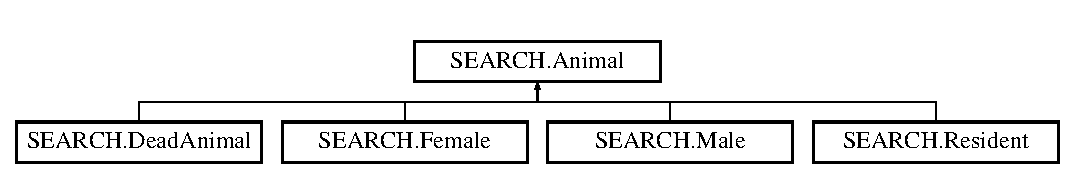
\includegraphics[height=1.958042cm]{class_s_e_a_r_c_h_1_1_animal}
\end{center}
\end{figure}
\subsection*{Public Member Functions}
\begin{DoxyCompactItemize}
\item 
\hyperlink{class_s_e_a_r_c_h_1_1_animal_aaa9f5d5d51a341abf19884abd2c0ee4c}{Animal} ()
\item 
void \hyperlink{class_s_e_a_r_c_h_1_1_animal_a622cf18a10d3e62e83b7063b7baa4189}{Build\-Text\-Writer} (string curr\-Year)
\item 
void \hyperlink{class_s_e_a_r_c_h_1_1_animal_a025bfbfcb038a9cd111fddb3f44a1082}{Build\-Text\-Writer} (string Curr\-Year, string Out\-Put\-Dir)
\item 
virtual void \hyperlink{class_s_e_a_r_c_h_1_1_animal_ad805d6441c4c873121136b641c404f3a}{do\-Time\-Step} (\hyperlink{class_s_e_a_r_c_h_1_1_hourly_modifier}{Hourly\-Modifier} in\-H\-M, \hyperlink{class_s_e_a_r_c_h_1_1_daily_modifier}{Daily\-Modifier} in\-D\-M, Date\-Time curr\-Time, bool do\-Text\-Output, ref string status)
\item 
virtual void \hyperlink{class_s_e_a_r_c_h_1_1_animal_ade2aab75e98f185a6f9ab2a5a9244bd3}{dump} ()
\item 
Point\-Class \hyperlink{class_s_e_a_r_c_h_1_1_animal_a303c52aede292098a8845d20a6a22cbf}{Get\-Eligible\-Step} (int step\-Num)
\item 
string \hyperlink{class_s_e_a_r_c_h_1_1_animal_aebe57edbaed290aa5d8131f99e69a6df}{get\-Location\-\_\-\-X\-Y} ()
\item 
int \hyperlink{class_s_e_a_r_c_h_1_1_animal_a5a9c4cc24c0989dd3d018d0231d3b160}{get\-Num\-Steps\-In\-Path} ()
\item 
bool \hyperlink{class_s_e_a_r_c_h_1_1_animal_ac7c6949790bf0be128c97d33f6131113}{is\-Site\-Good} ()
\item 
void \hyperlink{class_s_e_a_r_c_h_1_1_animal_aa7b2bbfe6c492ee6ab035ecdb16f8ce8}{set\-Initial\-Sleep\-Time} (Date\-Time curr\-Time)
\item 
void \hyperlink{class_s_e_a_r_c_h_1_1_animal_ad20fe454decc426f90750b45c2f0d28d}{set\-Initial\-Values} (Date\-Time curr\-Time)
\item 
void \hyperlink{class_s_e_a_r_c_h_1_1_animal_a1baf56f0f37d4e69f3252d76bfd4e530}{update\-Memory} ()
\end{DoxyCompactItemize}
\subsection*{Protected Member Functions}
\begin{DoxyCompactItemize}
\item 
void \hyperlink{class_s_e_a_r_c_h_1_1_animal_a0e3ffaa97d8155513f5e617972e42ef3}{build\-File\-Name\-Prefix} (string year)
\end{DoxyCompactItemize}
\subsection*{Protected Attributes}
\begin{DoxyCompactItemize}
\item 
bool \hyperlink{class_s_e_a_r_c_h_1_1_animal_a61211c92eed61826dffce1f84ef2e9f7}{m\-Is\-Dead}
\item 
string \hyperlink{class_s_e_a_r_c_h_1_1_animal_a6413b3476285ade80de97ff798445501}{sex}
\item 
\hyperlink{class_s_e_a_r_c_h_1_1_text_file_writer}{Text\-File\-Writer} \hyperlink{class_s_e_a_r_c_h_1_1_animal_adfbacc7101ae5d23be518f3adea3c894}{m\-Text\-File\-Writer}
\item 
\hyperlink{class_s_e_a_r_c_h_1_1_random_numbers}{Random\-Numbers} \hyperlink{class_s_e_a_r_c_h_1_1_animal_afbbfd34bac637b6560a90d91591b8288}{rn}
\end{DoxyCompactItemize}
\subsection*{Properties}
\begin{DoxyCompactItemize}
\item 
\hyperlink{class_s_e_a_r_c_h_1_1_home_range_criteria}{Home\-Range\-Criteria} \hyperlink{class_s_e_a_r_c_h_1_1_animal_acf76d8a9bcf386cc2a9720d10149d0a2}{Home\-Range\-Criteria}\hspace{0.3cm}{\ttfamily  \mbox{[}get, set\mbox{]}}
\item 
\hyperlink{class_s_e_a_r_c_h_1_1_animal_atributes}{Animal\-Atributes} \hyperlink{class_s_e_a_r_c_h_1_1_animal_afc8fe17408aa73f7a31f3e2409be79c5}{Animal\-Atributes}\hspace{0.3cm}{\ttfamily  \mbox{[}get, set\mbox{]}}
\item 
\hyperlink{class_s_e_a_r_c_h_1_1_animal_manager}{Animal\-Manager} \hyperlink{class_s_e_a_r_c_h_1_1_animal_a6a754d946c281c7e4d8f010c3b564223}{Animal\-Manager}\hspace{0.3cm}{\ttfamily  \mbox{[}get, set\mbox{]}}
\item 
double \hyperlink{class_s_e_a_r_c_h_1_1_animal_a2e672fd9d06e4dac3d5f9c6f19c0b914}{Capture\-Food}\hspace{0.3cm}{\ttfamily  \mbox{[}get, set\mbox{]}}
\item 
double \hyperlink{class_s_e_a_r_c_h_1_1_animal_ae8c02d56316874b56366bd7043d968f8}{Curr\-Energy}\hspace{0.3cm}{\ttfamily  \mbox{[}get, set\mbox{]}}
\item 
double \hyperlink{class_s_e_a_r_c_h_1_1_animal_af1d5e2abc62c1e11699c2733000df86b}{Energy\-Used}\hspace{0.3cm}{\ttfamily  \mbox{[}get, set\mbox{]}}
\item 
string \hyperlink{class_s_e_a_r_c_h_1_1_animal_ad354a9e9764c54e13a60a2a2555dee5f}{File\-Name\-Prefix}\hspace{0.3cm}{\ttfamily  \mbox{[}get\mbox{]}}
\item 
int \hyperlink{class_s_e_a_r_c_h_1_1_animal_a8f46a01a6a525b050106b7c33e23a6f6}{Food\-Index}\hspace{0.3cm}{\ttfamily  \mbox{[}get, set\mbox{]}}
\item 
double \hyperlink{class_s_e_a_r_c_h_1_1_animal_a047d41dbaec46762ba1d92f6a6658170}{Food\-Mean\-Size}\hspace{0.3cm}{\ttfamily  \mbox{[}get, set\mbox{]}}
\item 
double \hyperlink{class_s_e_a_r_c_h_1_1_animal_a0db89938a765aecd96e7f1d49aea6275}{Food\-S\-D\-\_\-\-Size}\hspace{0.3cm}{\ttfamily  \mbox{[}get, set\mbox{]}}
\item 
\hyperlink{class_s_e_a_r_c_h_1_1_modifier}{Modifier} \hyperlink{class_s_e_a_r_c_h_1_1_animal_aa114945a8096c6feec40c90132358373}{Gender\-Modifier}\hspace{0.3cm}{\ttfamily  \mbox{[}get, set\mbox{]}}
\item 
double \hyperlink{class_s_e_a_r_c_h_1_1_animal_ae97dc3434cb371a6afb6c2a4a66e998d}{Heading}\hspace{0.3cm}{\ttfamily  \mbox{[}get, set\mbox{]}}
\item 
Point\-Class \hyperlink{class_s_e_a_r_c_h_1_1_animal_a7f9bb5c7812e09103dd2ba1c544dc114}{Home\-Range\-Center}\hspace{0.3cm}{\ttfamily  \mbox{[}get, set\mbox{]}}
\item 
\hyperlink{interface_s_e_a_r_c_h_1_1_i_home_range_finder}{I\-Home\-Range\-Finder} \hyperlink{class_s_e_a_r_c_h_1_1_animal_af05446c781b60b5ecdc6fbd8d2d6508e}{Home\-Range\-Finder}\hspace{0.3cm}{\ttfamily  \mbox{[}get, set\mbox{]}}
\item 
\hyperlink{interface_s_e_a_r_c_h_1_1_i_home_range_trigger}{I\-Home\-Range\-Trigger} \hyperlink{class_s_e_a_r_c_h_1_1_animal_a11b0de2921f92d8fb4403c93321af158}{Home\-Range\-Trigger}\hspace{0.3cm}{\ttfamily  \mbox{[}get, set\mbox{]}}
\item 
int \hyperlink{class_s_e_a_r_c_h_1_1_animal_a71dc133a0902b560035c839eeab5aa5b}{Id\-Num}\hspace{0.3cm}{\ttfamily  \mbox{[}get, set\mbox{]}}
\item 
string \hyperlink{class_s_e_a_r_c_h_1_1_animal_afdb0155688bedee6cdea89a2ba9e416e}{Id\-Num\-Orig}\hspace{0.3cm}{\ttfamily  \mbox{[}get, set\mbox{]}}
\item 
bool \hyperlink{class_s_e_a_r_c_h_1_1_animal_a8560c12df05cfb9fd9552c2a6d6406d9}{Is\-Dead}\hspace{0.3cm}{\ttfamily  \mbox{[}get, set\mbox{]}}
\item 
I\-Point \hyperlink{class_s_e_a_r_c_h_1_1_animal_a268ceccff11bb7e97748f6fcc6f47850}{Location}\hspace{0.3cm}{\ttfamily  \mbox{[}get, set\mbox{]}}
\item 
\hyperlink{class_s_e_a_r_c_h_1_1_map_manager}{Map\-Manager} \hyperlink{class_s_e_a_r_c_h_1_1_animal_a7de0ff0d59e4f1a90e9bc78a8cfd1dd4}{Map\-Manager}\hspace{0.3cm}{\ttfamily  \mbox{[}get, set\mbox{]}}
\item 
int \hyperlink{class_s_e_a_r_c_h_1_1_animal_a331d43e7832be4c6bd92fac234c9d95d}{Move\-Index}\hspace{0.3cm}{\ttfamily  \mbox{[}get, set\mbox{]}}
\item 
double \hyperlink{class_s_e_a_r_c_h_1_1_animal_af81e361dcacc9d6885467e0e0d7d9333}{Move\-Speed}\hspace{0.3cm}{\ttfamily  \mbox{[}get, set\mbox{]}}
\item 
double \hyperlink{class_s_e_a_r_c_h_1_1_animal_ad5b3860044e5d6c935bf80f5de568595}{Move\-Turtosity}\hspace{0.3cm}{\ttfamily  \mbox{[}get, set\mbox{]}}
\item 
\hyperlink{class_s_e_a_r_c_h_1_1_mover}{Mover} \hyperlink{class_s_e_a_r_c_h_1_1_animal_a490ecc2f0acee533cfed4900abaec408}{my\-Mover}\hspace{0.3cm}{\ttfamily  \mbox{[}get, set\mbox{]}}
\item 
\hyperlink{class_s_e_a_r_c_h_1_1_eligible_home_sites}{Eligible\-Home\-Sites} \hyperlink{class_s_e_a_r_c_h_1_1_animal_a22a91ec4ec8cb552137231f5cc64a3d3}{My\-Visited\-Sites}\hspace{0.3cm}{\ttfamily  \mbox{[}get, set\mbox{]}}
\item 
double \hyperlink{class_s_e_a_r_c_h_1_1_animal_afa65021179183373fb9af5976b06fbf8}{Percepton\-Modifier}\hspace{0.3cm}{\ttfamily  \mbox{[}get, set\mbox{]}}
\item 
double \hyperlink{class_s_e_a_r_c_h_1_1_animal_a5753cc7dd073016ee6ad06a721039eda}{Predation\-Risk}\hspace{0.3cm}{\ttfamily  \mbox{[}get, set\mbox{]}}
\item 
int \hyperlink{class_s_e_a_r_c_h_1_1_animal_abf5587e6141d66bfef5d0e6e5e2b0249}{Risk\-Index}\hspace{0.3cm}{\ttfamily  \mbox{[}get, set\mbox{]}}
\item 
string \hyperlink{class_s_e_a_r_c_h_1_1_animal_a82057b36970fe4caf5df9f01cdec0c0b}{Sex}\hspace{0.3cm}{\ttfamily  \mbox{[}get, set\mbox{]}}
\item 
int \hyperlink{class_s_e_a_r_c_h_1_1_animal_a69680225461b7a1a5b4372cc9e6100e8}{Social\-Index}\hspace{0.3cm}{\ttfamily  \mbox{[}get, set\mbox{]}}
\item 
\hyperlink{class_s_e_a_r_c_h_1_1_modifier}{Modifier} \hyperlink{class_s_e_a_r_c_h_1_1_animal_acd1ded8fa372f9fce294354b95571b7e}{State\-Modifer}\hspace{0.3cm}{\ttfamily  \mbox{[}get, set\mbox{]}}
\item 
\hyperlink{class_s_e_a_r_c_h_1_1_text_file_writer}{Text\-File\-Writer} \hyperlink{class_s_e_a_r_c_h_1_1_animal_a0e2be0558719e097f07a996ac36d810e}{Text\-File\-Writer}\hspace{0.3cm}{\ttfamily  \mbox{[}get, set\mbox{]}}
\end{DoxyCompactItemize}


\subsection{Constructor \& Destructor Documentation}
\hypertarget{class_s_e_a_r_c_h_1_1_animal_aaa9f5d5d51a341abf19884abd2c0ee4c}{\index{S\-E\-A\-R\-C\-H\-::\-Animal@{S\-E\-A\-R\-C\-H\-::\-Animal}!Animal@{Animal}}
\index{Animal@{Animal}!SEARCH::Animal@{S\-E\-A\-R\-C\-H\-::\-Animal}}
\subsubsection[{Animal}]{\setlength{\rightskip}{0pt plus 5cm}S\-E\-A\-R\-C\-H.\-Animal.\-Animal (
\begin{DoxyParamCaption}
{}
\end{DoxyParamCaption}
)}}\label{class_s_e_a_r_c_h_1_1_animal_aaa9f5d5d51a341abf19884abd2c0ee4c}


\subsection{Member Function Documentation}
\hypertarget{class_s_e_a_r_c_h_1_1_animal_a0e3ffaa97d8155513f5e617972e42ef3}{\index{S\-E\-A\-R\-C\-H\-::\-Animal@{S\-E\-A\-R\-C\-H\-::\-Animal}!build\-File\-Name\-Prefix@{build\-File\-Name\-Prefix}}
\index{build\-File\-Name\-Prefix@{build\-File\-Name\-Prefix}!SEARCH::Animal@{S\-E\-A\-R\-C\-H\-::\-Animal}}
\subsubsection[{build\-File\-Name\-Prefix}]{\setlength{\rightskip}{0pt plus 5cm}void S\-E\-A\-R\-C\-H.\-Animal.\-build\-File\-Name\-Prefix (
\begin{DoxyParamCaption}
\item[{string}]{year}
\end{DoxyParamCaption}
)\hspace{0.3cm}{\ttfamily [protected]}}}\label{class_s_e_a_r_c_h_1_1_animal_a0e3ffaa97d8155513f5e617972e42ef3}
\hypertarget{class_s_e_a_r_c_h_1_1_animal_a622cf18a10d3e62e83b7063b7baa4189}{\index{S\-E\-A\-R\-C\-H\-::\-Animal@{S\-E\-A\-R\-C\-H\-::\-Animal}!Build\-Text\-Writer@{Build\-Text\-Writer}}
\index{Build\-Text\-Writer@{Build\-Text\-Writer}!SEARCH::Animal@{S\-E\-A\-R\-C\-H\-::\-Animal}}
\subsubsection[{Build\-Text\-Writer}]{\setlength{\rightskip}{0pt plus 5cm}void S\-E\-A\-R\-C\-H.\-Animal.\-Build\-Text\-Writer (
\begin{DoxyParamCaption}
\item[{string}]{curr\-Year}
\end{DoxyParamCaption}
)}}\label{class_s_e_a_r_c_h_1_1_animal_a622cf18a10d3e62e83b7063b7baa4189}
\hypertarget{class_s_e_a_r_c_h_1_1_animal_a025bfbfcb038a9cd111fddb3f44a1082}{\index{S\-E\-A\-R\-C\-H\-::\-Animal@{S\-E\-A\-R\-C\-H\-::\-Animal}!Build\-Text\-Writer@{Build\-Text\-Writer}}
\index{Build\-Text\-Writer@{Build\-Text\-Writer}!SEARCH::Animal@{S\-E\-A\-R\-C\-H\-::\-Animal}}
\subsubsection[{Build\-Text\-Writer}]{\setlength{\rightskip}{0pt plus 5cm}void S\-E\-A\-R\-C\-H.\-Animal.\-Build\-Text\-Writer (
\begin{DoxyParamCaption}
\item[{string}]{Curr\-Year, }
\item[{string}]{Out\-Put\-Dir}
\end{DoxyParamCaption}
)}}\label{class_s_e_a_r_c_h_1_1_animal_a025bfbfcb038a9cd111fddb3f44a1082}
\hypertarget{class_s_e_a_r_c_h_1_1_animal_ad805d6441c4c873121136b641c404f3a}{\index{S\-E\-A\-R\-C\-H\-::\-Animal@{S\-E\-A\-R\-C\-H\-::\-Animal}!do\-Time\-Step@{do\-Time\-Step}}
\index{do\-Time\-Step@{do\-Time\-Step}!SEARCH::Animal@{S\-E\-A\-R\-C\-H\-::\-Animal}}
\subsubsection[{do\-Time\-Step}]{\setlength{\rightskip}{0pt plus 5cm}virtual void S\-E\-A\-R\-C\-H.\-Animal.\-do\-Time\-Step (
\begin{DoxyParamCaption}
\item[{{\bf Hourly\-Modifier}}]{in\-H\-M, }
\item[{{\bf Daily\-Modifier}}]{in\-D\-M, }
\item[{Date\-Time}]{curr\-Time, }
\item[{bool}]{do\-Text\-Output, }
\item[{ref string}]{status}
\end{DoxyParamCaption}
)\hspace{0.3cm}{\ttfamily [virtual]}}}\label{class_s_e_a_r_c_h_1_1_animal_ad805d6441c4c873121136b641c404f3a}


Reimplemented in \hyperlink{class_s_e_a_r_c_h_1_1_resident_a8b8b9bf2d89bf08618b7649247c98da2}{S\-E\-A\-R\-C\-H.\-Resident}, and \hyperlink{class_s_e_a_r_c_h_1_1_dead_animal_a5a17ff4e63a89738621522de0658ae7b}{S\-E\-A\-R\-C\-H.\-Dead\-Animal}.

\hypertarget{class_s_e_a_r_c_h_1_1_animal_ade2aab75e98f185a6f9ab2a5a9244bd3}{\index{S\-E\-A\-R\-C\-H\-::\-Animal@{S\-E\-A\-R\-C\-H\-::\-Animal}!dump@{dump}}
\index{dump@{dump}!SEARCH::Animal@{S\-E\-A\-R\-C\-H\-::\-Animal}}
\subsubsection[{dump}]{\setlength{\rightskip}{0pt plus 5cm}virtual void S\-E\-A\-R\-C\-H.\-Animal.\-dump (
\begin{DoxyParamCaption}
{}
\end{DoxyParamCaption}
)\hspace{0.3cm}{\ttfamily [virtual]}}}\label{class_s_e_a_r_c_h_1_1_animal_ade2aab75e98f185a6f9ab2a5a9244bd3}


Reimplemented in \hyperlink{class_s_e_a_r_c_h_1_1_female_accc345d2bbf2a055b54f67df64a9cdc9}{S\-E\-A\-R\-C\-H.\-Female}, and \hyperlink{class_s_e_a_r_c_h_1_1_male_ae2c3be6f7a6daf01e72f2a7c6af0007e}{S\-E\-A\-R\-C\-H.\-Male}.

\hypertarget{class_s_e_a_r_c_h_1_1_animal_a303c52aede292098a8845d20a6a22cbf}{\index{S\-E\-A\-R\-C\-H\-::\-Animal@{S\-E\-A\-R\-C\-H\-::\-Animal}!Get\-Eligible\-Step@{Get\-Eligible\-Step}}
\index{Get\-Eligible\-Step@{Get\-Eligible\-Step}!SEARCH::Animal@{S\-E\-A\-R\-C\-H\-::\-Animal}}
\subsubsection[{Get\-Eligible\-Step}]{\setlength{\rightskip}{0pt plus 5cm}Point\-Class S\-E\-A\-R\-C\-H.\-Animal.\-Get\-Eligible\-Step (
\begin{DoxyParamCaption}
\item[{int}]{step\-Num}
\end{DoxyParamCaption}
)}}\label{class_s_e_a_r_c_h_1_1_animal_a303c52aede292098a8845d20a6a22cbf}
\hypertarget{class_s_e_a_r_c_h_1_1_animal_aebe57edbaed290aa5d8131f99e69a6df}{\index{S\-E\-A\-R\-C\-H\-::\-Animal@{S\-E\-A\-R\-C\-H\-::\-Animal}!get\-Location\-\_\-\-X\-Y@{get\-Location\-\_\-\-X\-Y}}
\index{get\-Location\-\_\-\-X\-Y@{get\-Location\-\_\-\-X\-Y}!SEARCH::Animal@{S\-E\-A\-R\-C\-H\-::\-Animal}}
\subsubsection[{get\-Location\-\_\-\-X\-Y}]{\setlength{\rightskip}{0pt plus 5cm}string S\-E\-A\-R\-C\-H.\-Animal.\-get\-Location\-\_\-\-X\-Y (
\begin{DoxyParamCaption}
{}
\end{DoxyParamCaption}
)}}\label{class_s_e_a_r_c_h_1_1_animal_aebe57edbaed290aa5d8131f99e69a6df}
\hypertarget{class_s_e_a_r_c_h_1_1_animal_a5a9c4cc24c0989dd3d018d0231d3b160}{\index{S\-E\-A\-R\-C\-H\-::\-Animal@{S\-E\-A\-R\-C\-H\-::\-Animal}!get\-Num\-Steps\-In\-Path@{get\-Num\-Steps\-In\-Path}}
\index{get\-Num\-Steps\-In\-Path@{get\-Num\-Steps\-In\-Path}!SEARCH::Animal@{S\-E\-A\-R\-C\-H\-::\-Animal}}
\subsubsection[{get\-Num\-Steps\-In\-Path}]{\setlength{\rightskip}{0pt plus 5cm}int S\-E\-A\-R\-C\-H.\-Animal.\-get\-Num\-Steps\-In\-Path (
\begin{DoxyParamCaption}
{}
\end{DoxyParamCaption}
)}}\label{class_s_e_a_r_c_h_1_1_animal_a5a9c4cc24c0989dd3d018d0231d3b160}
\hypertarget{class_s_e_a_r_c_h_1_1_animal_ac7c6949790bf0be128c97d33f6131113}{\index{S\-E\-A\-R\-C\-H\-::\-Animal@{S\-E\-A\-R\-C\-H\-::\-Animal}!is\-Site\-Good@{is\-Site\-Good}}
\index{is\-Site\-Good@{is\-Site\-Good}!SEARCH::Animal@{S\-E\-A\-R\-C\-H\-::\-Animal}}
\subsubsection[{is\-Site\-Good}]{\setlength{\rightskip}{0pt plus 5cm}bool S\-E\-A\-R\-C\-H.\-Animal.\-is\-Site\-Good (
\begin{DoxyParamCaption}
{}
\end{DoxyParamCaption}
)}}\label{class_s_e_a_r_c_h_1_1_animal_ac7c6949790bf0be128c97d33f6131113}
\hypertarget{class_s_e_a_r_c_h_1_1_animal_aa7b2bbfe6c492ee6ab035ecdb16f8ce8}{\index{S\-E\-A\-R\-C\-H\-::\-Animal@{S\-E\-A\-R\-C\-H\-::\-Animal}!set\-Initial\-Sleep\-Time@{set\-Initial\-Sleep\-Time}}
\index{set\-Initial\-Sleep\-Time@{set\-Initial\-Sleep\-Time}!SEARCH::Animal@{S\-E\-A\-R\-C\-H\-::\-Animal}}
\subsubsection[{set\-Initial\-Sleep\-Time}]{\setlength{\rightskip}{0pt plus 5cm}void S\-E\-A\-R\-C\-H.\-Animal.\-set\-Initial\-Sleep\-Time (
\begin{DoxyParamCaption}
\item[{Date\-Time}]{curr\-Time}
\end{DoxyParamCaption}
)}}\label{class_s_e_a_r_c_h_1_1_animal_aa7b2bbfe6c492ee6ab035ecdb16f8ce8}
\hypertarget{class_s_e_a_r_c_h_1_1_animal_ad20fe454decc426f90750b45c2f0d28d}{\index{S\-E\-A\-R\-C\-H\-::\-Animal@{S\-E\-A\-R\-C\-H\-::\-Animal}!set\-Initial\-Values@{set\-Initial\-Values}}
\index{set\-Initial\-Values@{set\-Initial\-Values}!SEARCH::Animal@{S\-E\-A\-R\-C\-H\-::\-Animal}}
\subsubsection[{set\-Initial\-Values}]{\setlength{\rightskip}{0pt plus 5cm}void S\-E\-A\-R\-C\-H.\-Animal.\-set\-Initial\-Values (
\begin{DoxyParamCaption}
\item[{Date\-Time}]{curr\-Time}
\end{DoxyParamCaption}
)}}\label{class_s_e_a_r_c_h_1_1_animal_ad20fe454decc426f90750b45c2f0d28d}
\hypertarget{class_s_e_a_r_c_h_1_1_animal_a1baf56f0f37d4e69f3252d76bfd4e530}{\index{S\-E\-A\-R\-C\-H\-::\-Animal@{S\-E\-A\-R\-C\-H\-::\-Animal}!update\-Memory@{update\-Memory}}
\index{update\-Memory@{update\-Memory}!SEARCH::Animal@{S\-E\-A\-R\-C\-H\-::\-Animal}}
\subsubsection[{update\-Memory}]{\setlength{\rightskip}{0pt plus 5cm}void S\-E\-A\-R\-C\-H.\-Animal.\-update\-Memory (
\begin{DoxyParamCaption}
{}
\end{DoxyParamCaption}
)}}\label{class_s_e_a_r_c_h_1_1_animal_a1baf56f0f37d4e69f3252d76bfd4e530}


\subsection{Member Data Documentation}
\hypertarget{class_s_e_a_r_c_h_1_1_animal_a61211c92eed61826dffce1f84ef2e9f7}{\index{S\-E\-A\-R\-C\-H\-::\-Animal@{S\-E\-A\-R\-C\-H\-::\-Animal}!m\-Is\-Dead@{m\-Is\-Dead}}
\index{m\-Is\-Dead@{m\-Is\-Dead}!SEARCH::Animal@{S\-E\-A\-R\-C\-H\-::\-Animal}}
\subsubsection[{m\-Is\-Dead}]{\setlength{\rightskip}{0pt plus 5cm}bool S\-E\-A\-R\-C\-H.\-Animal.\-m\-Is\-Dead\hspace{0.3cm}{\ttfamily [protected]}}}\label{class_s_e_a_r_c_h_1_1_animal_a61211c92eed61826dffce1f84ef2e9f7}
\hypertarget{class_s_e_a_r_c_h_1_1_animal_adfbacc7101ae5d23be518f3adea3c894}{\index{S\-E\-A\-R\-C\-H\-::\-Animal@{S\-E\-A\-R\-C\-H\-::\-Animal}!m\-Text\-File\-Writer@{m\-Text\-File\-Writer}}
\index{m\-Text\-File\-Writer@{m\-Text\-File\-Writer}!SEARCH::Animal@{S\-E\-A\-R\-C\-H\-::\-Animal}}
\subsubsection[{m\-Text\-File\-Writer}]{\setlength{\rightskip}{0pt plus 5cm}{\bf Text\-File\-Writer} S\-E\-A\-R\-C\-H.\-Animal.\-m\-Text\-File\-Writer\hspace{0.3cm}{\ttfamily [protected]}}}\label{class_s_e_a_r_c_h_1_1_animal_adfbacc7101ae5d23be518f3adea3c894}
\hypertarget{class_s_e_a_r_c_h_1_1_animal_afbbfd34bac637b6560a90d91591b8288}{\index{S\-E\-A\-R\-C\-H\-::\-Animal@{S\-E\-A\-R\-C\-H\-::\-Animal}!rn@{rn}}
\index{rn@{rn}!SEARCH::Animal@{S\-E\-A\-R\-C\-H\-::\-Animal}}
\subsubsection[{rn}]{\setlength{\rightskip}{0pt plus 5cm}{\bf Random\-Numbers} S\-E\-A\-R\-C\-H.\-Animal.\-rn\hspace{0.3cm}{\ttfamily [protected]}}}\label{class_s_e_a_r_c_h_1_1_animal_afbbfd34bac637b6560a90d91591b8288}
\hypertarget{class_s_e_a_r_c_h_1_1_animal_a6413b3476285ade80de97ff798445501}{\index{S\-E\-A\-R\-C\-H\-::\-Animal@{S\-E\-A\-R\-C\-H\-::\-Animal}!sex@{sex}}
\index{sex@{sex}!SEARCH::Animal@{S\-E\-A\-R\-C\-H\-::\-Animal}}
\subsubsection[{sex}]{\setlength{\rightskip}{0pt plus 5cm}string S\-E\-A\-R\-C\-H.\-Animal.\-sex\hspace{0.3cm}{\ttfamily [protected]}}}\label{class_s_e_a_r_c_h_1_1_animal_a6413b3476285ade80de97ff798445501}


\subsection{Property Documentation}
\hypertarget{class_s_e_a_r_c_h_1_1_animal_afc8fe17408aa73f7a31f3e2409be79c5}{\index{S\-E\-A\-R\-C\-H\-::\-Animal@{S\-E\-A\-R\-C\-H\-::\-Animal}!Animal\-Atributes@{Animal\-Atributes}}
\index{Animal\-Atributes@{Animal\-Atributes}!SEARCH::Animal@{S\-E\-A\-R\-C\-H\-::\-Animal}}
\subsubsection[{Animal\-Atributes}]{\setlength{\rightskip}{0pt plus 5cm}{\bf Animal\-Atributes} S\-E\-A\-R\-C\-H.\-Animal.\-Animal\-Atributes\hspace{0.3cm}{\ttfamily [get]}, {\ttfamily [set]}}}\label{class_s_e_a_r_c_h_1_1_animal_afc8fe17408aa73f7a31f3e2409be79c5}
\hypertarget{class_s_e_a_r_c_h_1_1_animal_a6a754d946c281c7e4d8f010c3b564223}{\index{S\-E\-A\-R\-C\-H\-::\-Animal@{S\-E\-A\-R\-C\-H\-::\-Animal}!Animal\-Manager@{Animal\-Manager}}
\index{Animal\-Manager@{Animal\-Manager}!SEARCH::Animal@{S\-E\-A\-R\-C\-H\-::\-Animal}}
\subsubsection[{Animal\-Manager}]{\setlength{\rightskip}{0pt plus 5cm}{\bf Animal\-Manager} S\-E\-A\-R\-C\-H.\-Animal.\-Animal\-Manager\hspace{0.3cm}{\ttfamily [get]}, {\ttfamily [set]}}}\label{class_s_e_a_r_c_h_1_1_animal_a6a754d946c281c7e4d8f010c3b564223}
\hypertarget{class_s_e_a_r_c_h_1_1_animal_a2e672fd9d06e4dac3d5f9c6f19c0b914}{\index{S\-E\-A\-R\-C\-H\-::\-Animal@{S\-E\-A\-R\-C\-H\-::\-Animal}!Capture\-Food@{Capture\-Food}}
\index{Capture\-Food@{Capture\-Food}!SEARCH::Animal@{S\-E\-A\-R\-C\-H\-::\-Animal}}
\subsubsection[{Capture\-Food}]{\setlength{\rightskip}{0pt plus 5cm}double S\-E\-A\-R\-C\-H.\-Animal.\-Capture\-Food\hspace{0.3cm}{\ttfamily [get]}, {\ttfamily [set]}}}\label{class_s_e_a_r_c_h_1_1_animal_a2e672fd9d06e4dac3d5f9c6f19c0b914}
\hypertarget{class_s_e_a_r_c_h_1_1_animal_ae8c02d56316874b56366bd7043d968f8}{\index{S\-E\-A\-R\-C\-H\-::\-Animal@{S\-E\-A\-R\-C\-H\-::\-Animal}!Curr\-Energy@{Curr\-Energy}}
\index{Curr\-Energy@{Curr\-Energy}!SEARCH::Animal@{S\-E\-A\-R\-C\-H\-::\-Animal}}
\subsubsection[{Curr\-Energy}]{\setlength{\rightskip}{0pt plus 5cm}double S\-E\-A\-R\-C\-H.\-Animal.\-Curr\-Energy\hspace{0.3cm}{\ttfamily [get]}, {\ttfamily [set]}}}\label{class_s_e_a_r_c_h_1_1_animal_ae8c02d56316874b56366bd7043d968f8}
\hypertarget{class_s_e_a_r_c_h_1_1_animal_af1d5e2abc62c1e11699c2733000df86b}{\index{S\-E\-A\-R\-C\-H\-::\-Animal@{S\-E\-A\-R\-C\-H\-::\-Animal}!Energy\-Used@{Energy\-Used}}
\index{Energy\-Used@{Energy\-Used}!SEARCH::Animal@{S\-E\-A\-R\-C\-H\-::\-Animal}}
\subsubsection[{Energy\-Used}]{\setlength{\rightskip}{0pt plus 5cm}double S\-E\-A\-R\-C\-H.\-Animal.\-Energy\-Used\hspace{0.3cm}{\ttfamily [get]}, {\ttfamily [set]}}}\label{class_s_e_a_r_c_h_1_1_animal_af1d5e2abc62c1e11699c2733000df86b}
\hypertarget{class_s_e_a_r_c_h_1_1_animal_ad354a9e9764c54e13a60a2a2555dee5f}{\index{S\-E\-A\-R\-C\-H\-::\-Animal@{S\-E\-A\-R\-C\-H\-::\-Animal}!File\-Name\-Prefix@{File\-Name\-Prefix}}
\index{File\-Name\-Prefix@{File\-Name\-Prefix}!SEARCH::Animal@{S\-E\-A\-R\-C\-H\-::\-Animal}}
\subsubsection[{File\-Name\-Prefix}]{\setlength{\rightskip}{0pt plus 5cm}string S\-E\-A\-R\-C\-H.\-Animal.\-File\-Name\-Prefix\hspace{0.3cm}{\ttfamily [get]}}}\label{class_s_e_a_r_c_h_1_1_animal_ad354a9e9764c54e13a60a2a2555dee5f}
\hypertarget{class_s_e_a_r_c_h_1_1_animal_a8f46a01a6a525b050106b7c33e23a6f6}{\index{S\-E\-A\-R\-C\-H\-::\-Animal@{S\-E\-A\-R\-C\-H\-::\-Animal}!Food\-Index@{Food\-Index}}
\index{Food\-Index@{Food\-Index}!SEARCH::Animal@{S\-E\-A\-R\-C\-H\-::\-Animal}}
\subsubsection[{Food\-Index}]{\setlength{\rightskip}{0pt plus 5cm}int S\-E\-A\-R\-C\-H.\-Animal.\-Food\-Index\hspace{0.3cm}{\ttfamily [get]}, {\ttfamily [set]}}}\label{class_s_e_a_r_c_h_1_1_animal_a8f46a01a6a525b050106b7c33e23a6f6}
\hypertarget{class_s_e_a_r_c_h_1_1_animal_a047d41dbaec46762ba1d92f6a6658170}{\index{S\-E\-A\-R\-C\-H\-::\-Animal@{S\-E\-A\-R\-C\-H\-::\-Animal}!Food\-Mean\-Size@{Food\-Mean\-Size}}
\index{Food\-Mean\-Size@{Food\-Mean\-Size}!SEARCH::Animal@{S\-E\-A\-R\-C\-H\-::\-Animal}}
\subsubsection[{Food\-Mean\-Size}]{\setlength{\rightskip}{0pt plus 5cm}double S\-E\-A\-R\-C\-H.\-Animal.\-Food\-Mean\-Size\hspace{0.3cm}{\ttfamily [get]}, {\ttfamily [set]}}}\label{class_s_e_a_r_c_h_1_1_animal_a047d41dbaec46762ba1d92f6a6658170}
\hypertarget{class_s_e_a_r_c_h_1_1_animal_a0db89938a765aecd96e7f1d49aea6275}{\index{S\-E\-A\-R\-C\-H\-::\-Animal@{S\-E\-A\-R\-C\-H\-::\-Animal}!Food\-S\-D\-\_\-\-Size@{Food\-S\-D\-\_\-\-Size}}
\index{Food\-S\-D\-\_\-\-Size@{Food\-S\-D\-\_\-\-Size}!SEARCH::Animal@{S\-E\-A\-R\-C\-H\-::\-Animal}}
\subsubsection[{Food\-S\-D\-\_\-\-Size}]{\setlength{\rightskip}{0pt plus 5cm}double S\-E\-A\-R\-C\-H.\-Animal.\-Food\-S\-D\-\_\-\-Size\hspace{0.3cm}{\ttfamily [get]}, {\ttfamily [set]}}}\label{class_s_e_a_r_c_h_1_1_animal_a0db89938a765aecd96e7f1d49aea6275}
\hypertarget{class_s_e_a_r_c_h_1_1_animal_aa114945a8096c6feec40c90132358373}{\index{S\-E\-A\-R\-C\-H\-::\-Animal@{S\-E\-A\-R\-C\-H\-::\-Animal}!Gender\-Modifier@{Gender\-Modifier}}
\index{Gender\-Modifier@{Gender\-Modifier}!SEARCH::Animal@{S\-E\-A\-R\-C\-H\-::\-Animal}}
\subsubsection[{Gender\-Modifier}]{\setlength{\rightskip}{0pt plus 5cm}{\bf Modifier} S\-E\-A\-R\-C\-H.\-Animal.\-Gender\-Modifier\hspace{0.3cm}{\ttfamily [get]}, {\ttfamily [set]}}}\label{class_s_e_a_r_c_h_1_1_animal_aa114945a8096c6feec40c90132358373}
\hypertarget{class_s_e_a_r_c_h_1_1_animal_ae97dc3434cb371a6afb6c2a4a66e998d}{\index{S\-E\-A\-R\-C\-H\-::\-Animal@{S\-E\-A\-R\-C\-H\-::\-Animal}!Heading@{Heading}}
\index{Heading@{Heading}!SEARCH::Animal@{S\-E\-A\-R\-C\-H\-::\-Animal}}
\subsubsection[{Heading}]{\setlength{\rightskip}{0pt plus 5cm}double S\-E\-A\-R\-C\-H.\-Animal.\-Heading\hspace{0.3cm}{\ttfamily [get]}, {\ttfamily [set]}}}\label{class_s_e_a_r_c_h_1_1_animal_ae97dc3434cb371a6afb6c2a4a66e998d}
\hypertarget{class_s_e_a_r_c_h_1_1_animal_a7f9bb5c7812e09103dd2ba1c544dc114}{\index{S\-E\-A\-R\-C\-H\-::\-Animal@{S\-E\-A\-R\-C\-H\-::\-Animal}!Home\-Range\-Center@{Home\-Range\-Center}}
\index{Home\-Range\-Center@{Home\-Range\-Center}!SEARCH::Animal@{S\-E\-A\-R\-C\-H\-::\-Animal}}
\subsubsection[{Home\-Range\-Center}]{\setlength{\rightskip}{0pt plus 5cm}Point\-Class S\-E\-A\-R\-C\-H.\-Animal.\-Home\-Range\-Center\hspace{0.3cm}{\ttfamily [get]}, {\ttfamily [set]}}}\label{class_s_e_a_r_c_h_1_1_animal_a7f9bb5c7812e09103dd2ba1c544dc114}
\hypertarget{class_s_e_a_r_c_h_1_1_animal_acf76d8a9bcf386cc2a9720d10149d0a2}{\index{S\-E\-A\-R\-C\-H\-::\-Animal@{S\-E\-A\-R\-C\-H\-::\-Animal}!Home\-Range\-Criteria@{Home\-Range\-Criteria}}
\index{Home\-Range\-Criteria@{Home\-Range\-Criteria}!SEARCH::Animal@{S\-E\-A\-R\-C\-H\-::\-Animal}}
\subsubsection[{Home\-Range\-Criteria}]{\setlength{\rightskip}{0pt plus 5cm}{\bf Home\-Range\-Criteria} S\-E\-A\-R\-C\-H.\-Animal.\-Home\-Range\-Criteria\hspace{0.3cm}{\ttfamily [get]}, {\ttfamily [set]}}}\label{class_s_e_a_r_c_h_1_1_animal_acf76d8a9bcf386cc2a9720d10149d0a2}
\hypertarget{class_s_e_a_r_c_h_1_1_animal_af05446c781b60b5ecdc6fbd8d2d6508e}{\index{S\-E\-A\-R\-C\-H\-::\-Animal@{S\-E\-A\-R\-C\-H\-::\-Animal}!Home\-Range\-Finder@{Home\-Range\-Finder}}
\index{Home\-Range\-Finder@{Home\-Range\-Finder}!SEARCH::Animal@{S\-E\-A\-R\-C\-H\-::\-Animal}}
\subsubsection[{Home\-Range\-Finder}]{\setlength{\rightskip}{0pt plus 5cm}{\bf I\-Home\-Range\-Finder} S\-E\-A\-R\-C\-H.\-Animal.\-Home\-Range\-Finder\hspace{0.3cm}{\ttfamily [get]}, {\ttfamily [set]}}}\label{class_s_e_a_r_c_h_1_1_animal_af05446c781b60b5ecdc6fbd8d2d6508e}
\hypertarget{class_s_e_a_r_c_h_1_1_animal_a11b0de2921f92d8fb4403c93321af158}{\index{S\-E\-A\-R\-C\-H\-::\-Animal@{S\-E\-A\-R\-C\-H\-::\-Animal}!Home\-Range\-Trigger@{Home\-Range\-Trigger}}
\index{Home\-Range\-Trigger@{Home\-Range\-Trigger}!SEARCH::Animal@{S\-E\-A\-R\-C\-H\-::\-Animal}}
\subsubsection[{Home\-Range\-Trigger}]{\setlength{\rightskip}{0pt plus 5cm}{\bf I\-Home\-Range\-Trigger} S\-E\-A\-R\-C\-H.\-Animal.\-Home\-Range\-Trigger\hspace{0.3cm}{\ttfamily [get]}, {\ttfamily [set]}}}\label{class_s_e_a_r_c_h_1_1_animal_a11b0de2921f92d8fb4403c93321af158}
\hypertarget{class_s_e_a_r_c_h_1_1_animal_a71dc133a0902b560035c839eeab5aa5b}{\index{S\-E\-A\-R\-C\-H\-::\-Animal@{S\-E\-A\-R\-C\-H\-::\-Animal}!Id\-Num@{Id\-Num}}
\index{Id\-Num@{Id\-Num}!SEARCH::Animal@{S\-E\-A\-R\-C\-H\-::\-Animal}}
\subsubsection[{Id\-Num}]{\setlength{\rightskip}{0pt plus 5cm}int S\-E\-A\-R\-C\-H.\-Animal.\-Id\-Num\hspace{0.3cm}{\ttfamily [get]}, {\ttfamily [set]}}}\label{class_s_e_a_r_c_h_1_1_animal_a71dc133a0902b560035c839eeab5aa5b}
\hypertarget{class_s_e_a_r_c_h_1_1_animal_afdb0155688bedee6cdea89a2ba9e416e}{\index{S\-E\-A\-R\-C\-H\-::\-Animal@{S\-E\-A\-R\-C\-H\-::\-Animal}!Id\-Num\-Orig@{Id\-Num\-Orig}}
\index{Id\-Num\-Orig@{Id\-Num\-Orig}!SEARCH::Animal@{S\-E\-A\-R\-C\-H\-::\-Animal}}
\subsubsection[{Id\-Num\-Orig}]{\setlength{\rightskip}{0pt plus 5cm}string S\-E\-A\-R\-C\-H.\-Animal.\-Id\-Num\-Orig\hspace{0.3cm}{\ttfamily [get]}, {\ttfamily [set]}}}\label{class_s_e_a_r_c_h_1_1_animal_afdb0155688bedee6cdea89a2ba9e416e}
\hypertarget{class_s_e_a_r_c_h_1_1_animal_a8560c12df05cfb9fd9552c2a6d6406d9}{\index{S\-E\-A\-R\-C\-H\-::\-Animal@{S\-E\-A\-R\-C\-H\-::\-Animal}!Is\-Dead@{Is\-Dead}}
\index{Is\-Dead@{Is\-Dead}!SEARCH::Animal@{S\-E\-A\-R\-C\-H\-::\-Animal}}
\subsubsection[{Is\-Dead}]{\setlength{\rightskip}{0pt plus 5cm}bool S\-E\-A\-R\-C\-H.\-Animal.\-Is\-Dead\hspace{0.3cm}{\ttfamily [get]}, {\ttfamily [set]}}}\label{class_s_e_a_r_c_h_1_1_animal_a8560c12df05cfb9fd9552c2a6d6406d9}
\hypertarget{class_s_e_a_r_c_h_1_1_animal_a268ceccff11bb7e97748f6fcc6f47850}{\index{S\-E\-A\-R\-C\-H\-::\-Animal@{S\-E\-A\-R\-C\-H\-::\-Animal}!Location@{Location}}
\index{Location@{Location}!SEARCH::Animal@{S\-E\-A\-R\-C\-H\-::\-Animal}}
\subsubsection[{Location}]{\setlength{\rightskip}{0pt plus 5cm}I\-Point S\-E\-A\-R\-C\-H.\-Animal.\-Location\hspace{0.3cm}{\ttfamily [get]}, {\ttfamily [set]}}}\label{class_s_e_a_r_c_h_1_1_animal_a268ceccff11bb7e97748f6fcc6f47850}
\hypertarget{class_s_e_a_r_c_h_1_1_animal_a7de0ff0d59e4f1a90e9bc78a8cfd1dd4}{\index{S\-E\-A\-R\-C\-H\-::\-Animal@{S\-E\-A\-R\-C\-H\-::\-Animal}!Map\-Manager@{Map\-Manager}}
\index{Map\-Manager@{Map\-Manager}!SEARCH::Animal@{S\-E\-A\-R\-C\-H\-::\-Animal}}
\subsubsection[{Map\-Manager}]{\setlength{\rightskip}{0pt plus 5cm}{\bf Map\-Manager} S\-E\-A\-R\-C\-H.\-Animal.\-Map\-Manager\hspace{0.3cm}{\ttfamily [get]}, {\ttfamily [set]}}}\label{class_s_e_a_r_c_h_1_1_animal_a7de0ff0d59e4f1a90e9bc78a8cfd1dd4}
\hypertarget{class_s_e_a_r_c_h_1_1_animal_a331d43e7832be4c6bd92fac234c9d95d}{\index{S\-E\-A\-R\-C\-H\-::\-Animal@{S\-E\-A\-R\-C\-H\-::\-Animal}!Move\-Index@{Move\-Index}}
\index{Move\-Index@{Move\-Index}!SEARCH::Animal@{S\-E\-A\-R\-C\-H\-::\-Animal}}
\subsubsection[{Move\-Index}]{\setlength{\rightskip}{0pt plus 5cm}int S\-E\-A\-R\-C\-H.\-Animal.\-Move\-Index\hspace{0.3cm}{\ttfamily [get]}, {\ttfamily [set]}}}\label{class_s_e_a_r_c_h_1_1_animal_a331d43e7832be4c6bd92fac234c9d95d}
\hypertarget{class_s_e_a_r_c_h_1_1_animal_af81e361dcacc9d6885467e0e0d7d9333}{\index{S\-E\-A\-R\-C\-H\-::\-Animal@{S\-E\-A\-R\-C\-H\-::\-Animal}!Move\-Speed@{Move\-Speed}}
\index{Move\-Speed@{Move\-Speed}!SEARCH::Animal@{S\-E\-A\-R\-C\-H\-::\-Animal}}
\subsubsection[{Move\-Speed}]{\setlength{\rightskip}{0pt plus 5cm}double S\-E\-A\-R\-C\-H.\-Animal.\-Move\-Speed\hspace{0.3cm}{\ttfamily [get]}, {\ttfamily [set]}}}\label{class_s_e_a_r_c_h_1_1_animal_af81e361dcacc9d6885467e0e0d7d9333}
\hypertarget{class_s_e_a_r_c_h_1_1_animal_ad5b3860044e5d6c935bf80f5de568595}{\index{S\-E\-A\-R\-C\-H\-::\-Animal@{S\-E\-A\-R\-C\-H\-::\-Animal}!Move\-Turtosity@{Move\-Turtosity}}
\index{Move\-Turtosity@{Move\-Turtosity}!SEARCH::Animal@{S\-E\-A\-R\-C\-H\-::\-Animal}}
\subsubsection[{Move\-Turtosity}]{\setlength{\rightskip}{0pt plus 5cm}double S\-E\-A\-R\-C\-H.\-Animal.\-Move\-Turtosity\hspace{0.3cm}{\ttfamily [get]}, {\ttfamily [set]}}}\label{class_s_e_a_r_c_h_1_1_animal_ad5b3860044e5d6c935bf80f5de568595}
\hypertarget{class_s_e_a_r_c_h_1_1_animal_a490ecc2f0acee533cfed4900abaec408}{\index{S\-E\-A\-R\-C\-H\-::\-Animal@{S\-E\-A\-R\-C\-H\-::\-Animal}!my\-Mover@{my\-Mover}}
\index{my\-Mover@{my\-Mover}!SEARCH::Animal@{S\-E\-A\-R\-C\-H\-::\-Animal}}
\subsubsection[{my\-Mover}]{\setlength{\rightskip}{0pt plus 5cm}{\bf Mover} S\-E\-A\-R\-C\-H.\-Animal.\-my\-Mover\hspace{0.3cm}{\ttfamily [get]}, {\ttfamily [set]}}}\label{class_s_e_a_r_c_h_1_1_animal_a490ecc2f0acee533cfed4900abaec408}
\hypertarget{class_s_e_a_r_c_h_1_1_animal_a22a91ec4ec8cb552137231f5cc64a3d3}{\index{S\-E\-A\-R\-C\-H\-::\-Animal@{S\-E\-A\-R\-C\-H\-::\-Animal}!My\-Visited\-Sites@{My\-Visited\-Sites}}
\index{My\-Visited\-Sites@{My\-Visited\-Sites}!SEARCH::Animal@{S\-E\-A\-R\-C\-H\-::\-Animal}}
\subsubsection[{My\-Visited\-Sites}]{\setlength{\rightskip}{0pt plus 5cm}{\bf Eligible\-Home\-Sites} S\-E\-A\-R\-C\-H.\-Animal.\-My\-Visited\-Sites\hspace{0.3cm}{\ttfamily [get]}, {\ttfamily [set]}}}\label{class_s_e_a_r_c_h_1_1_animal_a22a91ec4ec8cb552137231f5cc64a3d3}
\hypertarget{class_s_e_a_r_c_h_1_1_animal_afa65021179183373fb9af5976b06fbf8}{\index{S\-E\-A\-R\-C\-H\-::\-Animal@{S\-E\-A\-R\-C\-H\-::\-Animal}!Percepton\-Modifier@{Percepton\-Modifier}}
\index{Percepton\-Modifier@{Percepton\-Modifier}!SEARCH::Animal@{S\-E\-A\-R\-C\-H\-::\-Animal}}
\subsubsection[{Percepton\-Modifier}]{\setlength{\rightskip}{0pt plus 5cm}double S\-E\-A\-R\-C\-H.\-Animal.\-Percepton\-Modifier\hspace{0.3cm}{\ttfamily [get]}, {\ttfamily [set]}}}\label{class_s_e_a_r_c_h_1_1_animal_afa65021179183373fb9af5976b06fbf8}
\hypertarget{class_s_e_a_r_c_h_1_1_animal_a5753cc7dd073016ee6ad06a721039eda}{\index{S\-E\-A\-R\-C\-H\-::\-Animal@{S\-E\-A\-R\-C\-H\-::\-Animal}!Predation\-Risk@{Predation\-Risk}}
\index{Predation\-Risk@{Predation\-Risk}!SEARCH::Animal@{S\-E\-A\-R\-C\-H\-::\-Animal}}
\subsubsection[{Predation\-Risk}]{\setlength{\rightskip}{0pt plus 5cm}double S\-E\-A\-R\-C\-H.\-Animal.\-Predation\-Risk\hspace{0.3cm}{\ttfamily [get]}, {\ttfamily [set]}}}\label{class_s_e_a_r_c_h_1_1_animal_a5753cc7dd073016ee6ad06a721039eda}
\hypertarget{class_s_e_a_r_c_h_1_1_animal_abf5587e6141d66bfef5d0e6e5e2b0249}{\index{S\-E\-A\-R\-C\-H\-::\-Animal@{S\-E\-A\-R\-C\-H\-::\-Animal}!Risk\-Index@{Risk\-Index}}
\index{Risk\-Index@{Risk\-Index}!SEARCH::Animal@{S\-E\-A\-R\-C\-H\-::\-Animal}}
\subsubsection[{Risk\-Index}]{\setlength{\rightskip}{0pt plus 5cm}int S\-E\-A\-R\-C\-H.\-Animal.\-Risk\-Index\hspace{0.3cm}{\ttfamily [get]}, {\ttfamily [set]}}}\label{class_s_e_a_r_c_h_1_1_animal_abf5587e6141d66bfef5d0e6e5e2b0249}
\hypertarget{class_s_e_a_r_c_h_1_1_animal_a82057b36970fe4caf5df9f01cdec0c0b}{\index{S\-E\-A\-R\-C\-H\-::\-Animal@{S\-E\-A\-R\-C\-H\-::\-Animal}!Sex@{Sex}}
\index{Sex@{Sex}!SEARCH::Animal@{S\-E\-A\-R\-C\-H\-::\-Animal}}
\subsubsection[{Sex}]{\setlength{\rightskip}{0pt plus 5cm}string S\-E\-A\-R\-C\-H.\-Animal.\-Sex\hspace{0.3cm}{\ttfamily [get]}, {\ttfamily [set]}}}\label{class_s_e_a_r_c_h_1_1_animal_a82057b36970fe4caf5df9f01cdec0c0b}
\hypertarget{class_s_e_a_r_c_h_1_1_animal_a69680225461b7a1a5b4372cc9e6100e8}{\index{S\-E\-A\-R\-C\-H\-::\-Animal@{S\-E\-A\-R\-C\-H\-::\-Animal}!Social\-Index@{Social\-Index}}
\index{Social\-Index@{Social\-Index}!SEARCH::Animal@{S\-E\-A\-R\-C\-H\-::\-Animal}}
\subsubsection[{Social\-Index}]{\setlength{\rightskip}{0pt plus 5cm}int S\-E\-A\-R\-C\-H.\-Animal.\-Social\-Index\hspace{0.3cm}{\ttfamily [get]}, {\ttfamily [set]}}}\label{class_s_e_a_r_c_h_1_1_animal_a69680225461b7a1a5b4372cc9e6100e8}
\hypertarget{class_s_e_a_r_c_h_1_1_animal_acd1ded8fa372f9fce294354b95571b7e}{\index{S\-E\-A\-R\-C\-H\-::\-Animal@{S\-E\-A\-R\-C\-H\-::\-Animal}!State\-Modifer@{State\-Modifer}}
\index{State\-Modifer@{State\-Modifer}!SEARCH::Animal@{S\-E\-A\-R\-C\-H\-::\-Animal}}
\subsubsection[{State\-Modifer}]{\setlength{\rightskip}{0pt plus 5cm}{\bf Modifier} S\-E\-A\-R\-C\-H.\-Animal.\-State\-Modifer\hspace{0.3cm}{\ttfamily [get]}, {\ttfamily [set]}}}\label{class_s_e_a_r_c_h_1_1_animal_acd1ded8fa372f9fce294354b95571b7e}
\hypertarget{class_s_e_a_r_c_h_1_1_animal_a0e2be0558719e097f07a996ac36d810e}{\index{S\-E\-A\-R\-C\-H\-::\-Animal@{S\-E\-A\-R\-C\-H\-::\-Animal}!Text\-File\-Writer@{Text\-File\-Writer}}
\index{Text\-File\-Writer@{Text\-File\-Writer}!SEARCH::Animal@{S\-E\-A\-R\-C\-H\-::\-Animal}}
\subsubsection[{Text\-File\-Writer}]{\setlength{\rightskip}{0pt plus 5cm}{\bf Text\-File\-Writer} S\-E\-A\-R\-C\-H.\-Animal.\-Text\-File\-Writer\hspace{0.3cm}{\ttfamily [get]}, {\ttfamily [set]}}}\label{class_s_e_a_r_c_h_1_1_animal_a0e2be0558719e097f07a996ac36d810e}


The documentation for this class was generated from the following file\-:\begin{DoxyCompactItemize}
\item 
Desktop/vlog4net\-A\-R\-C10\-\_\-64\-\_\-newhoming/\-Data\-Centric/\hyperlink{_animal_8cs}{Animal.\-cs}\end{DoxyCompactItemize}

\hypertarget{class_s_e_a_r_c_h_1_1_animal_atributes}{\section{S\-E\-A\-R\-C\-H.\-Animal\-Atributes Class Reference}
\label{class_s_e_a_r_c_h_1_1_animal_atributes}\index{S\-E\-A\-R\-C\-H.\-Animal\-Atributes@{S\-E\-A\-R\-C\-H.\-Animal\-Atributes}}
}


Attributes for a gender/species combination animal  


\subsection*{Public Member Functions}
\begin{DoxyCompactItemize}
\item 
\hyperlink{class_s_e_a_r_c_h_1_1_animal_atributes_a6f43f288ff9ef744b76d6ee1a2b62be2}{Animal\-Atributes} ()
\item 
double \hyperlink{class_s_e_a_r_c_h_1_1_animal_atributes_a97cd28150a5f6108de05568db7d34c88}{add\-Duration} (\hyperlink{struct_s_e_a_r_c_h_1_1_duration}{Duration} in\-D)
\item 
void \hyperlink{class_s_e_a_r_c_h_1_1_animal_atributes_a23d709722ba91ea5e24ce7779c82e234}{get\-Duration\-Mean\-And\-S\-D} (ref double mean, ref double sd, ref int duration\-I\-D)
\end{DoxyCompactItemize}
\subsection*{Properties}
\begin{DoxyCompactItemize}
\item 
\hyperlink{struct_s_e_a_r_c_h_1_1_duration}{Duration}\mbox{[}$\,$\mbox{]} \hyperlink{class_s_e_a_r_c_h_1_1_animal_atributes_afc7aba890c91bb4c436e673bf7116fea}{Activity\-Durations}\hspace{0.3cm}{\ttfamily  \mbox{[}get\mbox{]}}
\item 
string \hyperlink{class_s_e_a_r_c_h_1_1_animal_atributes_a218579d75b3d4f852b84da4d6d8e26ca}{Out\-Put\-Dir}\hspace{0.3cm}{\ttfamily  \mbox{[}get, set\mbox{]}}
\item 
double \hyperlink{class_s_e_a_r_c_h_1_1_animal_atributes_af2f0d37e12632e12d51e6d42e702cc46}{Initial\-Energy}\hspace{0.3cm}{\ttfamily  \mbox{[}get, set\mbox{]}}
\item 
double \hyperlink{class_s_e_a_r_c_h_1_1_animal_atributes_aa18e55c7dc93db227993bdf5b02e0f81}{Max\-Energy}\hspace{0.3cm}{\ttfamily  \mbox{[}get, set\mbox{]}}
\item 
double \hyperlink{class_s_e_a_r_c_h_1_1_animal_atributes_adb822e897a7275d39c7475f551d29145}{Min\-Energy\-\_\-\-Survive}\hspace{0.3cm}{\ttfamily  \mbox{[}get, set\mbox{]}}
\item 
double \hyperlink{class_s_e_a_r_c_h_1_1_animal_atributes_ac891cd39725f29fc85c265c432c1fa3e}{Wake\-Up\-Time}\hspace{0.3cm}{\ttfamily  \mbox{[}get, set\mbox{]}}
\item 
double \hyperlink{class_s_e_a_r_c_h_1_1_animal_atributes_a46f40d9ec1c7909a8d9ca2712b260513}{Perception\-Distance}\hspace{0.3cm}{\ttfamily  \mbox{[}get, set\mbox{]}}
\item 
double \hyperlink{class_s_e_a_r_c_h_1_1_animal_atributes_a147ee1f1277ac9a820446277e3c73533}{Forage\-Search\-Trigger}\hspace{0.3cm}{\ttfamily  \mbox{[}get, set\mbox{]}}
\item 
double \hyperlink{class_s_e_a_r_c_h_1_1_animal_atributes_a179e48f031efc0a8bdbd126fecd75b9f}{Risky\-Safe\-Trigger}\hspace{0.3cm}{\ttfamily  \mbox{[}get, set\mbox{]}}
\item 
double \hyperlink{class_s_e_a_r_c_h_1_1_animal_atributes_a61865dd6afeb2c1c45347f5d7cf3e3d4}{Safe\-Risky\-Trigger}\hspace{0.3cm}{\ttfamily  \mbox{[}get, set\mbox{]}}
\item 
string \hyperlink{class_s_e_a_r_c_h_1_1_animal_atributes_a07e3e4068701076d76126bb59aba3a59}{Err\-Message}\hspace{0.3cm}{\ttfamily  \mbox{[}get, set\mbox{]}}
\item 
double \hyperlink{class_s_e_a_r_c_h_1_1_animal_atributes_a9a21b4bd7d1d6ff6968015cb85477d00}{Safe\-Prob\-Capture\-Food\-Mod}\hspace{0.3cm}{\ttfamily  \mbox{[}get, set\mbox{]}}
\item 
double \hyperlink{class_s_e_a_r_c_h_1_1_animal_atributes_af316458962100c38806cf2a9a4a2a9c6}{Safe\-Prob\-Get\-Killed\-Mod}\hspace{0.3cm}{\ttfamily  \mbox{[}get, set\mbox{]}}
\item 
double \hyperlink{class_s_e_a_r_c_h_1_1_animal_atributes_a04cb4aa140730cebbdcfdd35dd6c51fe}{Risky\-Prob\-Capture\-Food\-Mod}\hspace{0.3cm}{\ttfamily  \mbox{[}get, set\mbox{]}}
\item 
double \hyperlink{class_s_e_a_r_c_h_1_1_animal_atributes_a55782572243807106661327e9c8a255b}{Risky\-Prob\-Get\-Killed\-Mod}\hspace{0.3cm}{\ttfamily  \mbox{[}get, set\mbox{]}}
\end{DoxyCompactItemize}


\subsection{Detailed Description}
Attributes for a gender/species combination animal 



\subsection{Constructor \& Destructor Documentation}
\hypertarget{class_s_e_a_r_c_h_1_1_animal_atributes_a6f43f288ff9ef744b76d6ee1a2b62be2}{\index{S\-E\-A\-R\-C\-H\-::\-Animal\-Atributes@{S\-E\-A\-R\-C\-H\-::\-Animal\-Atributes}!Animal\-Atributes@{Animal\-Atributes}}
\index{Animal\-Atributes@{Animal\-Atributes}!SEARCH::AnimalAtributes@{S\-E\-A\-R\-C\-H\-::\-Animal\-Atributes}}
\subsubsection[{Animal\-Atributes}]{\setlength{\rightskip}{0pt plus 5cm}S\-E\-A\-R\-C\-H.\-Animal\-Atributes.\-Animal\-Atributes (
\begin{DoxyParamCaption}
{}
\end{DoxyParamCaption}
)}}\label{class_s_e_a_r_c_h_1_1_animal_atributes_a6f43f288ff9ef744b76d6ee1a2b62be2}


\subsection{Member Function Documentation}
\hypertarget{class_s_e_a_r_c_h_1_1_animal_atributes_a97cd28150a5f6108de05568db7d34c88}{\index{S\-E\-A\-R\-C\-H\-::\-Animal\-Atributes@{S\-E\-A\-R\-C\-H\-::\-Animal\-Atributes}!add\-Duration@{add\-Duration}}
\index{add\-Duration@{add\-Duration}!SEARCH::AnimalAtributes@{S\-E\-A\-R\-C\-H\-::\-Animal\-Atributes}}
\subsubsection[{add\-Duration}]{\setlength{\rightskip}{0pt plus 5cm}double S\-E\-A\-R\-C\-H.\-Animal\-Atributes.\-add\-Duration (
\begin{DoxyParamCaption}
\item[{{\bf Duration}}]{in\-D}
\end{DoxyParamCaption}
)}}\label{class_s_e_a_r_c_h_1_1_animal_atributes_a97cd28150a5f6108de05568db7d34c88}
\hypertarget{class_s_e_a_r_c_h_1_1_animal_atributes_a23d709722ba91ea5e24ce7779c82e234}{\index{S\-E\-A\-R\-C\-H\-::\-Animal\-Atributes@{S\-E\-A\-R\-C\-H\-::\-Animal\-Atributes}!get\-Duration\-Mean\-And\-S\-D@{get\-Duration\-Mean\-And\-S\-D}}
\index{get\-Duration\-Mean\-And\-S\-D@{get\-Duration\-Mean\-And\-S\-D}!SEARCH::AnimalAtributes@{S\-E\-A\-R\-C\-H\-::\-Animal\-Atributes}}
\subsubsection[{get\-Duration\-Mean\-And\-S\-D}]{\setlength{\rightskip}{0pt plus 5cm}void S\-E\-A\-R\-C\-H.\-Animal\-Atributes.\-get\-Duration\-Mean\-And\-S\-D (
\begin{DoxyParamCaption}
\item[{ref double}]{mean, }
\item[{ref double}]{sd, }
\item[{ref int}]{duration\-I\-D}
\end{DoxyParamCaption}
)}}\label{class_s_e_a_r_c_h_1_1_animal_atributes_a23d709722ba91ea5e24ce7779c82e234}


\subsection{Property Documentation}
\hypertarget{class_s_e_a_r_c_h_1_1_animal_atributes_afc7aba890c91bb4c436e673bf7116fea}{\index{S\-E\-A\-R\-C\-H\-::\-Animal\-Atributes@{S\-E\-A\-R\-C\-H\-::\-Animal\-Atributes}!Activity\-Durations@{Activity\-Durations}}
\index{Activity\-Durations@{Activity\-Durations}!SEARCH::AnimalAtributes@{S\-E\-A\-R\-C\-H\-::\-Animal\-Atributes}}
\subsubsection[{Activity\-Durations}]{\setlength{\rightskip}{0pt plus 5cm}{\bf Duration} \mbox{[}$\,$\mbox{]} S\-E\-A\-R\-C\-H.\-Animal\-Atributes.\-Activity\-Durations\hspace{0.3cm}{\ttfamily [get]}}}\label{class_s_e_a_r_c_h_1_1_animal_atributes_afc7aba890c91bb4c436e673bf7116fea}
\hypertarget{class_s_e_a_r_c_h_1_1_animal_atributes_a07e3e4068701076d76126bb59aba3a59}{\index{S\-E\-A\-R\-C\-H\-::\-Animal\-Atributes@{S\-E\-A\-R\-C\-H\-::\-Animal\-Atributes}!Err\-Message@{Err\-Message}}
\index{Err\-Message@{Err\-Message}!SEARCH::AnimalAtributes@{S\-E\-A\-R\-C\-H\-::\-Animal\-Atributes}}
\subsubsection[{Err\-Message}]{\setlength{\rightskip}{0pt plus 5cm}string S\-E\-A\-R\-C\-H.\-Animal\-Atributes.\-Err\-Message\hspace{0.3cm}{\ttfamily [get]}, {\ttfamily [set]}}}\label{class_s_e_a_r_c_h_1_1_animal_atributes_a07e3e4068701076d76126bb59aba3a59}
\hypertarget{class_s_e_a_r_c_h_1_1_animal_atributes_a147ee1f1277ac9a820446277e3c73533}{\index{S\-E\-A\-R\-C\-H\-::\-Animal\-Atributes@{S\-E\-A\-R\-C\-H\-::\-Animal\-Atributes}!Forage\-Search\-Trigger@{Forage\-Search\-Trigger}}
\index{Forage\-Search\-Trigger@{Forage\-Search\-Trigger}!SEARCH::AnimalAtributes@{S\-E\-A\-R\-C\-H\-::\-Animal\-Atributes}}
\subsubsection[{Forage\-Search\-Trigger}]{\setlength{\rightskip}{0pt plus 5cm}double S\-E\-A\-R\-C\-H.\-Animal\-Atributes.\-Forage\-Search\-Trigger\hspace{0.3cm}{\ttfamily [get]}, {\ttfamily [set]}}}\label{class_s_e_a_r_c_h_1_1_animal_atributes_a147ee1f1277ac9a820446277e3c73533}
\hypertarget{class_s_e_a_r_c_h_1_1_animal_atributes_af2f0d37e12632e12d51e6d42e702cc46}{\index{S\-E\-A\-R\-C\-H\-::\-Animal\-Atributes@{S\-E\-A\-R\-C\-H\-::\-Animal\-Atributes}!Initial\-Energy@{Initial\-Energy}}
\index{Initial\-Energy@{Initial\-Energy}!SEARCH::AnimalAtributes@{S\-E\-A\-R\-C\-H\-::\-Animal\-Atributes}}
\subsubsection[{Initial\-Energy}]{\setlength{\rightskip}{0pt plus 5cm}double S\-E\-A\-R\-C\-H.\-Animal\-Atributes.\-Initial\-Energy\hspace{0.3cm}{\ttfamily [get]}, {\ttfamily [set]}}}\label{class_s_e_a_r_c_h_1_1_animal_atributes_af2f0d37e12632e12d51e6d42e702cc46}
\hypertarget{class_s_e_a_r_c_h_1_1_animal_atributes_aa18e55c7dc93db227993bdf5b02e0f81}{\index{S\-E\-A\-R\-C\-H\-::\-Animal\-Atributes@{S\-E\-A\-R\-C\-H\-::\-Animal\-Atributes}!Max\-Energy@{Max\-Energy}}
\index{Max\-Energy@{Max\-Energy}!SEARCH::AnimalAtributes@{S\-E\-A\-R\-C\-H\-::\-Animal\-Atributes}}
\subsubsection[{Max\-Energy}]{\setlength{\rightskip}{0pt plus 5cm}double S\-E\-A\-R\-C\-H.\-Animal\-Atributes.\-Max\-Energy\hspace{0.3cm}{\ttfamily [get]}, {\ttfamily [set]}}}\label{class_s_e_a_r_c_h_1_1_animal_atributes_aa18e55c7dc93db227993bdf5b02e0f81}
\hypertarget{class_s_e_a_r_c_h_1_1_animal_atributes_adb822e897a7275d39c7475f551d29145}{\index{S\-E\-A\-R\-C\-H\-::\-Animal\-Atributes@{S\-E\-A\-R\-C\-H\-::\-Animal\-Atributes}!Min\-Energy\-\_\-\-Survive@{Min\-Energy\-\_\-\-Survive}}
\index{Min\-Energy\-\_\-\-Survive@{Min\-Energy\-\_\-\-Survive}!SEARCH::AnimalAtributes@{S\-E\-A\-R\-C\-H\-::\-Animal\-Atributes}}
\subsubsection[{Min\-Energy\-\_\-\-Survive}]{\setlength{\rightskip}{0pt plus 5cm}double S\-E\-A\-R\-C\-H.\-Animal\-Atributes.\-Min\-Energy\-\_\-\-Survive\hspace{0.3cm}{\ttfamily [get]}, {\ttfamily [set]}}}\label{class_s_e_a_r_c_h_1_1_animal_atributes_adb822e897a7275d39c7475f551d29145}
\hypertarget{class_s_e_a_r_c_h_1_1_animal_atributes_a218579d75b3d4f852b84da4d6d8e26ca}{\index{S\-E\-A\-R\-C\-H\-::\-Animal\-Atributes@{S\-E\-A\-R\-C\-H\-::\-Animal\-Atributes}!Out\-Put\-Dir@{Out\-Put\-Dir}}
\index{Out\-Put\-Dir@{Out\-Put\-Dir}!SEARCH::AnimalAtributes@{S\-E\-A\-R\-C\-H\-::\-Animal\-Atributes}}
\subsubsection[{Out\-Put\-Dir}]{\setlength{\rightskip}{0pt plus 5cm}string S\-E\-A\-R\-C\-H.\-Animal\-Atributes.\-Out\-Put\-Dir\hspace{0.3cm}{\ttfamily [get]}, {\ttfamily [set]}}}\label{class_s_e_a_r_c_h_1_1_animal_atributes_a218579d75b3d4f852b84da4d6d8e26ca}
\hypertarget{class_s_e_a_r_c_h_1_1_animal_atributes_a46f40d9ec1c7909a8d9ca2712b260513}{\index{S\-E\-A\-R\-C\-H\-::\-Animal\-Atributes@{S\-E\-A\-R\-C\-H\-::\-Animal\-Atributes}!Perception\-Distance@{Perception\-Distance}}
\index{Perception\-Distance@{Perception\-Distance}!SEARCH::AnimalAtributes@{S\-E\-A\-R\-C\-H\-::\-Animal\-Atributes}}
\subsubsection[{Perception\-Distance}]{\setlength{\rightskip}{0pt plus 5cm}double S\-E\-A\-R\-C\-H.\-Animal\-Atributes.\-Perception\-Distance\hspace{0.3cm}{\ttfamily [get]}, {\ttfamily [set]}}}\label{class_s_e_a_r_c_h_1_1_animal_atributes_a46f40d9ec1c7909a8d9ca2712b260513}
\hypertarget{class_s_e_a_r_c_h_1_1_animal_atributes_a04cb4aa140730cebbdcfdd35dd6c51fe}{\index{S\-E\-A\-R\-C\-H\-::\-Animal\-Atributes@{S\-E\-A\-R\-C\-H\-::\-Animal\-Atributes}!Risky\-Prob\-Capture\-Food\-Mod@{Risky\-Prob\-Capture\-Food\-Mod}}
\index{Risky\-Prob\-Capture\-Food\-Mod@{Risky\-Prob\-Capture\-Food\-Mod}!SEARCH::AnimalAtributes@{S\-E\-A\-R\-C\-H\-::\-Animal\-Atributes}}
\subsubsection[{Risky\-Prob\-Capture\-Food\-Mod}]{\setlength{\rightskip}{0pt plus 5cm}double S\-E\-A\-R\-C\-H.\-Animal\-Atributes.\-Risky\-Prob\-Capture\-Food\-Mod\hspace{0.3cm}{\ttfamily [get]}, {\ttfamily [set]}}}\label{class_s_e_a_r_c_h_1_1_animal_atributes_a04cb4aa140730cebbdcfdd35dd6c51fe}
\hypertarget{class_s_e_a_r_c_h_1_1_animal_atributes_a55782572243807106661327e9c8a255b}{\index{S\-E\-A\-R\-C\-H\-::\-Animal\-Atributes@{S\-E\-A\-R\-C\-H\-::\-Animal\-Atributes}!Risky\-Prob\-Get\-Killed\-Mod@{Risky\-Prob\-Get\-Killed\-Mod}}
\index{Risky\-Prob\-Get\-Killed\-Mod@{Risky\-Prob\-Get\-Killed\-Mod}!SEARCH::AnimalAtributes@{S\-E\-A\-R\-C\-H\-::\-Animal\-Atributes}}
\subsubsection[{Risky\-Prob\-Get\-Killed\-Mod}]{\setlength{\rightskip}{0pt plus 5cm}double S\-E\-A\-R\-C\-H.\-Animal\-Atributes.\-Risky\-Prob\-Get\-Killed\-Mod\hspace{0.3cm}{\ttfamily [get]}, {\ttfamily [set]}}}\label{class_s_e_a_r_c_h_1_1_animal_atributes_a55782572243807106661327e9c8a255b}
\hypertarget{class_s_e_a_r_c_h_1_1_animal_atributes_a179e48f031efc0a8bdbd126fecd75b9f}{\index{S\-E\-A\-R\-C\-H\-::\-Animal\-Atributes@{S\-E\-A\-R\-C\-H\-::\-Animal\-Atributes}!Risky\-Safe\-Trigger@{Risky\-Safe\-Trigger}}
\index{Risky\-Safe\-Trigger@{Risky\-Safe\-Trigger}!SEARCH::AnimalAtributes@{S\-E\-A\-R\-C\-H\-::\-Animal\-Atributes}}
\subsubsection[{Risky\-Safe\-Trigger}]{\setlength{\rightskip}{0pt plus 5cm}double S\-E\-A\-R\-C\-H.\-Animal\-Atributes.\-Risky\-Safe\-Trigger\hspace{0.3cm}{\ttfamily [get]}, {\ttfamily [set]}}}\label{class_s_e_a_r_c_h_1_1_animal_atributes_a179e48f031efc0a8bdbd126fecd75b9f}
\hypertarget{class_s_e_a_r_c_h_1_1_animal_atributes_a9a21b4bd7d1d6ff6968015cb85477d00}{\index{S\-E\-A\-R\-C\-H\-::\-Animal\-Atributes@{S\-E\-A\-R\-C\-H\-::\-Animal\-Atributes}!Safe\-Prob\-Capture\-Food\-Mod@{Safe\-Prob\-Capture\-Food\-Mod}}
\index{Safe\-Prob\-Capture\-Food\-Mod@{Safe\-Prob\-Capture\-Food\-Mod}!SEARCH::AnimalAtributes@{S\-E\-A\-R\-C\-H\-::\-Animal\-Atributes}}
\subsubsection[{Safe\-Prob\-Capture\-Food\-Mod}]{\setlength{\rightskip}{0pt plus 5cm}double S\-E\-A\-R\-C\-H.\-Animal\-Atributes.\-Safe\-Prob\-Capture\-Food\-Mod\hspace{0.3cm}{\ttfamily [get]}, {\ttfamily [set]}}}\label{class_s_e_a_r_c_h_1_1_animal_atributes_a9a21b4bd7d1d6ff6968015cb85477d00}
\hypertarget{class_s_e_a_r_c_h_1_1_animal_atributes_af316458962100c38806cf2a9a4a2a9c6}{\index{S\-E\-A\-R\-C\-H\-::\-Animal\-Atributes@{S\-E\-A\-R\-C\-H\-::\-Animal\-Atributes}!Safe\-Prob\-Get\-Killed\-Mod@{Safe\-Prob\-Get\-Killed\-Mod}}
\index{Safe\-Prob\-Get\-Killed\-Mod@{Safe\-Prob\-Get\-Killed\-Mod}!SEARCH::AnimalAtributes@{S\-E\-A\-R\-C\-H\-::\-Animal\-Atributes}}
\subsubsection[{Safe\-Prob\-Get\-Killed\-Mod}]{\setlength{\rightskip}{0pt plus 5cm}double S\-E\-A\-R\-C\-H.\-Animal\-Atributes.\-Safe\-Prob\-Get\-Killed\-Mod\hspace{0.3cm}{\ttfamily [get]}, {\ttfamily [set]}}}\label{class_s_e_a_r_c_h_1_1_animal_atributes_af316458962100c38806cf2a9a4a2a9c6}
\hypertarget{class_s_e_a_r_c_h_1_1_animal_atributes_a61865dd6afeb2c1c45347f5d7cf3e3d4}{\index{S\-E\-A\-R\-C\-H\-::\-Animal\-Atributes@{S\-E\-A\-R\-C\-H\-::\-Animal\-Atributes}!Safe\-Risky\-Trigger@{Safe\-Risky\-Trigger}}
\index{Safe\-Risky\-Trigger@{Safe\-Risky\-Trigger}!SEARCH::AnimalAtributes@{S\-E\-A\-R\-C\-H\-::\-Animal\-Atributes}}
\subsubsection[{Safe\-Risky\-Trigger}]{\setlength{\rightskip}{0pt plus 5cm}double S\-E\-A\-R\-C\-H.\-Animal\-Atributes.\-Safe\-Risky\-Trigger\hspace{0.3cm}{\ttfamily [get]}, {\ttfamily [set]}}}\label{class_s_e_a_r_c_h_1_1_animal_atributes_a61865dd6afeb2c1c45347f5d7cf3e3d4}
\hypertarget{class_s_e_a_r_c_h_1_1_animal_atributes_ac891cd39725f29fc85c265c432c1fa3e}{\index{S\-E\-A\-R\-C\-H\-::\-Animal\-Atributes@{S\-E\-A\-R\-C\-H\-::\-Animal\-Atributes}!Wake\-Up\-Time@{Wake\-Up\-Time}}
\index{Wake\-Up\-Time@{Wake\-Up\-Time}!SEARCH::AnimalAtributes@{S\-E\-A\-R\-C\-H\-::\-Animal\-Atributes}}
\subsubsection[{Wake\-Up\-Time}]{\setlength{\rightskip}{0pt plus 5cm}double S\-E\-A\-R\-C\-H.\-Animal\-Atributes.\-Wake\-Up\-Time\hspace{0.3cm}{\ttfamily [get]}, {\ttfamily [set]}}}\label{class_s_e_a_r_c_h_1_1_animal_atributes_ac891cd39725f29fc85c265c432c1fa3e}


The documentation for this class was generated from the following file\-:\begin{DoxyCompactItemize}
\item 
Desktop/vlog4net\-A\-R\-C10\-\_\-64\-\_\-newhoming/\-Data\-Centric/\hyperlink{_animal_atributes_8cs}{Animal\-Atributes.\-cs}\end{DoxyCompactItemize}

\hypertarget{class_s_e_a_r_c_h_1_1_animal_manager}{\section{S\-E\-A\-R\-C\-H.\-Animal\-Manager Class Reference}
\label{class_s_e_a_r_c_h_1_1_animal_manager}\index{S\-E\-A\-R\-C\-H.\-Animal\-Manager@{S\-E\-A\-R\-C\-H.\-Animal\-Manager}}
}
\subsection*{Public Member Functions}
\begin{DoxyCompactItemize}
\item 
\hyperlink{class_s_e_a_r_c_h_1_1_animal_manager_ab06ac6961b7e2e54209cd69799613b16}{Animal\-Manager} ()
\item 
int \hyperlink{class_s_e_a_r_c_h_1_1_animal_manager_af3d578bc12adec2c51f3ffd3d322f957}{get\-Num\-Dispersers} ()
\item 
int \hyperlink{class_s_e_a_r_c_h_1_1_animal_manager_add6db1dd2dfaa4335a508dd8357f6e3f}{get\-Num\-Residents} ()
\item 
void \hyperlink{class_s_e_a_r_c_h_1_1_animal_manager_a7d7b49737303ee1f5bb9e6774c2d1421}{add\-New\-Dispersers} (\hyperlink{class_s_e_a_r_c_h_1_1_initial_animal_attributes}{Initial\-Animal\-Attributes}\mbox{[}$\,$\mbox{]} in\-I\-A\-A, Date\-Time curr\-Time)
\item 
void \hyperlink{class_s_e_a_r_c_h_1_1_animal_manager_ac83809e22ce75662e738c06cb6b3f97a}{adjust\-New\-Social\-Map} (\hyperlink{class_s_e_a_r_c_h_1_1_map}{Map} new\-Social\-Map)
\item 
int \hyperlink{class_s_e_a_r_c_h_1_1_animal_manager_a09b650261c078d2435b8fe022b6fc19e}{breed\-Females} (Date\-Time curr\-Time)
\item 
void \hyperlink{class_s_e_a_r_c_h_1_1_animal_manager_aba58794e113743b4a8708e0b99a63fe2}{change\-To\-Dead\-Animal} (\hyperlink{class_s_e_a_r_c_h_1_1_animal}{Animal} in\-A)
\item 
void \hyperlink{class_s_e_a_r_c_h_1_1_animal_manager_a935cde1ac6704e8535d45746b64a3eb8}{do\-Time\-Step} (\hyperlink{class_s_e_a_r_c_h_1_1_hourly_modifier}{Hourly\-Modifier} in\-H\-M, \hyperlink{class_s_e_a_r_c_h_1_1_daily_modifier}{Daily\-Modifier} in\-D\-M, Date\-Time curr\-Time, bool Do\-Text\-Out\-Put, \hyperlink{class_s_e_a_r_c_h_1_1_map}{Map} curr\-Social\-Map)
\item 
void \hyperlink{class_s_e_a_r_c_h_1_1_animal_manager_a95e8ebd52daa94bac6c3b8cdad28512c}{dump} ()
\item 
String\-Collection \hyperlink{class_s_e_a_r_c_h_1_1_animal_manager_a031aa25ed9a846b311c03fdc471c43b9}{get\-Resident\-I\-Ds} ()
\item 
bool \hyperlink{class_s_e_a_r_c_h_1_1_animal_manager_a094207a7ccfbb164a70c04d656e4abd4}{make\-Initial\-Animals} (\hyperlink{class_s_e_a_r_c_h_1_1_initial_animal_attributes}{Initial\-Animal\-Attributes}\mbox{[}$\,$\mbox{]} in\-I\-A\-A)
\item 
bool \hyperlink{class_s_e_a_r_c_h_1_1_animal_manager_abfbe471dbe58fa2b56c0e353832369d7}{make\-Residents} (\hyperlink{class_s_e_a_r_c_h_1_1_initial_animal_attributes}{Initial\-Animal\-Attributes}\mbox{[}$\,$\mbox{]}in\-Res\-Attributes, string curr\-Year)
\item 
void \hyperlink{class_s_e_a_r_c_h_1_1_animal_manager_a050fac140af923a69fa649cfa8d77c93}{remove\-Remaing\-Dispersers} ()
\item 
bool \hyperlink{class_s_e_a_r_c_h_1_1_animal_manager_aa980efa432568bc8f7089e196834bf0b}{set\-Attributes} ()
\item 
void \hyperlink{class_s_e_a_r_c_h_1_1_animal_manager_a5757f4786a35939a635bdbc42dc96af0}{set\-Home\-Range} (string sex, double area, double distance\-Mean, double distance\-S\-D, double distance\-Weight)
\item 
bool \hyperlink{class_s_e_a_r_c_h_1_1_animal_manager_adb607f1396228db4657023b5395bb872}{set\-Home\-Range\-Criteria} (string type)
\item 
void \hyperlink{class_s_e_a_r_c_h_1_1_animal_manager_a45b122d488534474f9824e4bd58bfa54}{set\-Home\-Range\-Trigger} (string type, int num)
\item 
bool \hyperlink{class_s_e_a_r_c_h_1_1_animal_manager_ab0c4db81bb8b9152af18b2b2263a2684}{set\-Modifiers} ()
\item 
void \hyperlink{class_s_e_a_r_c_h_1_1_animal_manager_a0239f416e2332da5288e4cae87984d8a}{set\-Resident\-Modifier\-Values} (double in\-Time\-Step\-Risk, double in\-Yearly\-Risk, double in\-Percent\-Breed, double in\-Percent\-Female, double in\-Mean\-Litter\-Size, double in\-S\-D\-Litter\-Size)
\item 
bool \hyperlink{class_s_e_a_r_c_h_1_1_animal_manager_a707210bc35dde5c75c0601116b71e1ff}{set\-Sleep\-Time} (Date\-Time curr\-Time)
\item 
void \hyperlink{class_s_e_a_r_c_h_1_1_animal_manager_a04a6d2cfcda981b0c2775f7f3d1fa652}{winter\-Kill\-Residents} (\hyperlink{class_s_e_a_r_c_h_1_1_map}{Map} curr\-Social\-Map, int current\-Time)
\item 
void \hyperlink{class_s_e_a_r_c_h_1_1_animal_manager_af1f2d68341a4cfef2d8c8e8ad487e58e}{set\-Residents\-Text\-Output} (string path, string year)
\end{DoxyCompactItemize}
\subsection*{Properties}
\begin{DoxyCompactItemize}
\item 
\hyperlink{class_s_e_a_r_c_h_1_1_animal_atributes}{Animal\-Atributes} \hyperlink{class_s_e_a_r_c_h_1_1_animal_manager_a8349d00f52614df2284bb8ffba935b9c}{Animal\-Attributes}\hspace{0.3cm}{\ttfamily  \mbox{[}get, set\mbox{]}}
\item 
string \hyperlink{class_s_e_a_r_c_h_1_1_animal_manager_acc1cd13b6562447578772c34c0db2f6d}{Err\-Message}\hspace{0.3cm}{\ttfamily  \mbox{[}get, set\mbox{]}}
\item 
\hyperlink{class_s_e_a_r_c_h_1_1_female_modifier}{Female\-Modifier} \hyperlink{class_s_e_a_r_c_h_1_1_animal_manager_a40397d04d9d33fe1ee68b401f3e2c2b0}{Female\-Modifier}\hspace{0.3cm}{\ttfamily  \mbox{[}get, set\mbox{]}}
\item 
\hyperlink{class_s_e_a_r_c_h_1_1_male_modifier}{Male\-Modifier} \hyperlink{class_s_e_a_r_c_h_1_1_animal_manager_a104145af738786e1ff56fad9bbfffe8f}{Male\-Modifier}\hspace{0.3cm}{\ttfamily  \mbox{[}get, set\mbox{]}}
\item 
\hyperlink{class_s_e_a_r_c_h_1_1_resident_attributes}{Resident\-Attributes} \hyperlink{class_s_e_a_r_c_h_1_1_animal_manager_a4a34a6f225d2b9ba7adf762583ba6ec0}{Resident\-Attributes}\hspace{0.3cm}{\ttfamily  \mbox{[}get, set\mbox{]}}
\item 
\hyperlink{class_s_e_a_r_c_h_1_1_modifier}{Modifier} \hyperlink{class_s_e_a_r_c_h_1_1_animal_manager_a7c95f633caf112e185d2059bad7b21b5}{Risky\-Forage\-Mod}\hspace{0.3cm}{\ttfamily  \mbox{[}get, set\mbox{]}}
\item 
\hyperlink{class_s_e_a_r_c_h_1_1_modifier}{Modifier} \hyperlink{class_s_e_a_r_c_h_1_1_animal_manager_abcaa8f634b294977cbeb077717ed8961}{Risky\-Search\-Mod}\hspace{0.3cm}{\ttfamily  \mbox{[}get, set\mbox{]}}
\item 
\hyperlink{class_s_e_a_r_c_h_1_1_modifier}{Modifier} \hyperlink{class_s_e_a_r_c_h_1_1_animal_manager_a38061cc4a1441dc32e0d76d067439206}{Safe\-Forage\-Mod}\hspace{0.3cm}{\ttfamily  \mbox{[}get, set\mbox{]}}
\item 
\hyperlink{class_s_e_a_r_c_h_1_1_modifier}{Modifier} \hyperlink{class_s_e_a_r_c_h_1_1_animal_manager_a1343854b00d8b64b3ab607f8aaf75795}{Safe\-Search\-Mod}\hspace{0.3cm}{\ttfamily  \mbox{[}get, set\mbox{]}}
\end{DoxyCompactItemize}


\subsection{Constructor \& Destructor Documentation}
\hypertarget{class_s_e_a_r_c_h_1_1_animal_manager_ab06ac6961b7e2e54209cd69799613b16}{\index{S\-E\-A\-R\-C\-H\-::\-Animal\-Manager@{S\-E\-A\-R\-C\-H\-::\-Animal\-Manager}!Animal\-Manager@{Animal\-Manager}}
\index{Animal\-Manager@{Animal\-Manager}!SEARCH::AnimalManager@{S\-E\-A\-R\-C\-H\-::\-Animal\-Manager}}
\subsubsection[{Animal\-Manager}]{\setlength{\rightskip}{0pt plus 5cm}S\-E\-A\-R\-C\-H.\-Animal\-Manager.\-Animal\-Manager (
\begin{DoxyParamCaption}
{}
\end{DoxyParamCaption}
)}}\label{class_s_e_a_r_c_h_1_1_animal_manager_ab06ac6961b7e2e54209cd69799613b16}


\subsection{Member Function Documentation}
\hypertarget{class_s_e_a_r_c_h_1_1_animal_manager_a7d7b49737303ee1f5bb9e6774c2d1421}{\index{S\-E\-A\-R\-C\-H\-::\-Animal\-Manager@{S\-E\-A\-R\-C\-H\-::\-Animal\-Manager}!add\-New\-Dispersers@{add\-New\-Dispersers}}
\index{add\-New\-Dispersers@{add\-New\-Dispersers}!SEARCH::AnimalManager@{S\-E\-A\-R\-C\-H\-::\-Animal\-Manager}}
\subsubsection[{add\-New\-Dispersers}]{\setlength{\rightskip}{0pt plus 5cm}void S\-E\-A\-R\-C\-H.\-Animal\-Manager.\-add\-New\-Dispersers (
\begin{DoxyParamCaption}
\item[{{\bf Initial\-Animal\-Attributes}\mbox{[}$\,$\mbox{]}}]{in\-I\-A\-A, }
\item[{Date\-Time}]{curr\-Time}
\end{DoxyParamCaption}
)}}\label{class_s_e_a_r_c_h_1_1_animal_manager_a7d7b49737303ee1f5bb9e6774c2d1421}
\hypertarget{class_s_e_a_r_c_h_1_1_animal_manager_ac83809e22ce75662e738c06cb6b3f97a}{\index{S\-E\-A\-R\-C\-H\-::\-Animal\-Manager@{S\-E\-A\-R\-C\-H\-::\-Animal\-Manager}!adjust\-New\-Social\-Map@{adjust\-New\-Social\-Map}}
\index{adjust\-New\-Social\-Map@{adjust\-New\-Social\-Map}!SEARCH::AnimalManager@{S\-E\-A\-R\-C\-H\-::\-Animal\-Manager}}
\subsubsection[{adjust\-New\-Social\-Map}]{\setlength{\rightskip}{0pt plus 5cm}void S\-E\-A\-R\-C\-H.\-Animal\-Manager.\-adjust\-New\-Social\-Map (
\begin{DoxyParamCaption}
\item[{{\bf Map}}]{new\-Social\-Map}
\end{DoxyParamCaption}
)}}\label{class_s_e_a_r_c_h_1_1_animal_manager_ac83809e22ce75662e738c06cb6b3f97a}
\hypertarget{class_s_e_a_r_c_h_1_1_animal_manager_a09b650261c078d2435b8fe022b6fc19e}{\index{S\-E\-A\-R\-C\-H\-::\-Animal\-Manager@{S\-E\-A\-R\-C\-H\-::\-Animal\-Manager}!breed\-Females@{breed\-Females}}
\index{breed\-Females@{breed\-Females}!SEARCH::AnimalManager@{S\-E\-A\-R\-C\-H\-::\-Animal\-Manager}}
\subsubsection[{breed\-Females}]{\setlength{\rightskip}{0pt plus 5cm}int S\-E\-A\-R\-C\-H.\-Animal\-Manager.\-breed\-Females (
\begin{DoxyParamCaption}
\item[{Date\-Time}]{curr\-Time}
\end{DoxyParamCaption}
)}}\label{class_s_e_a_r_c_h_1_1_animal_manager_a09b650261c078d2435b8fe022b6fc19e}
\hypertarget{class_s_e_a_r_c_h_1_1_animal_manager_aba58794e113743b4a8708e0b99a63fe2}{\index{S\-E\-A\-R\-C\-H\-::\-Animal\-Manager@{S\-E\-A\-R\-C\-H\-::\-Animal\-Manager}!change\-To\-Dead\-Animal@{change\-To\-Dead\-Animal}}
\index{change\-To\-Dead\-Animal@{change\-To\-Dead\-Animal}!SEARCH::AnimalManager@{S\-E\-A\-R\-C\-H\-::\-Animal\-Manager}}
\subsubsection[{change\-To\-Dead\-Animal}]{\setlength{\rightskip}{0pt plus 5cm}void S\-E\-A\-R\-C\-H.\-Animal\-Manager.\-change\-To\-Dead\-Animal (
\begin{DoxyParamCaption}
\item[{{\bf Animal}}]{in\-A}
\end{DoxyParamCaption}
)}}\label{class_s_e_a_r_c_h_1_1_animal_manager_aba58794e113743b4a8708e0b99a63fe2}
\hypertarget{class_s_e_a_r_c_h_1_1_animal_manager_a935cde1ac6704e8535d45746b64a3eb8}{\index{S\-E\-A\-R\-C\-H\-::\-Animal\-Manager@{S\-E\-A\-R\-C\-H\-::\-Animal\-Manager}!do\-Time\-Step@{do\-Time\-Step}}
\index{do\-Time\-Step@{do\-Time\-Step}!SEARCH::AnimalManager@{S\-E\-A\-R\-C\-H\-::\-Animal\-Manager}}
\subsubsection[{do\-Time\-Step}]{\setlength{\rightskip}{0pt plus 5cm}void S\-E\-A\-R\-C\-H.\-Animal\-Manager.\-do\-Time\-Step (
\begin{DoxyParamCaption}
\item[{{\bf Hourly\-Modifier}}]{in\-H\-M, }
\item[{{\bf Daily\-Modifier}}]{in\-D\-M, }
\item[{Date\-Time}]{curr\-Time, }
\item[{bool}]{Do\-Text\-Out\-Put, }
\item[{{\bf Map}}]{curr\-Social\-Map}
\end{DoxyParamCaption}
)}}\label{class_s_e_a_r_c_h_1_1_animal_manager_a935cde1ac6704e8535d45746b64a3eb8}
\hypertarget{class_s_e_a_r_c_h_1_1_animal_manager_a95e8ebd52daa94bac6c3b8cdad28512c}{\index{S\-E\-A\-R\-C\-H\-::\-Animal\-Manager@{S\-E\-A\-R\-C\-H\-::\-Animal\-Manager}!dump@{dump}}
\index{dump@{dump}!SEARCH::AnimalManager@{S\-E\-A\-R\-C\-H\-::\-Animal\-Manager}}
\subsubsection[{dump}]{\setlength{\rightskip}{0pt plus 5cm}void S\-E\-A\-R\-C\-H.\-Animal\-Manager.\-dump (
\begin{DoxyParamCaption}
{}
\end{DoxyParamCaption}
)}}\label{class_s_e_a_r_c_h_1_1_animal_manager_a95e8ebd52daa94bac6c3b8cdad28512c}
\hypertarget{class_s_e_a_r_c_h_1_1_animal_manager_af3d578bc12adec2c51f3ffd3d322f957}{\index{S\-E\-A\-R\-C\-H\-::\-Animal\-Manager@{S\-E\-A\-R\-C\-H\-::\-Animal\-Manager}!get\-Num\-Dispersers@{get\-Num\-Dispersers}}
\index{get\-Num\-Dispersers@{get\-Num\-Dispersers}!SEARCH::AnimalManager@{S\-E\-A\-R\-C\-H\-::\-Animal\-Manager}}
\subsubsection[{get\-Num\-Dispersers}]{\setlength{\rightskip}{0pt plus 5cm}int S\-E\-A\-R\-C\-H.\-Animal\-Manager.\-get\-Num\-Dispersers (
\begin{DoxyParamCaption}
{}
\end{DoxyParamCaption}
)}}\label{class_s_e_a_r_c_h_1_1_animal_manager_af3d578bc12adec2c51f3ffd3d322f957}
\hypertarget{class_s_e_a_r_c_h_1_1_animal_manager_add6db1dd2dfaa4335a508dd8357f6e3f}{\index{S\-E\-A\-R\-C\-H\-::\-Animal\-Manager@{S\-E\-A\-R\-C\-H\-::\-Animal\-Manager}!get\-Num\-Residents@{get\-Num\-Residents}}
\index{get\-Num\-Residents@{get\-Num\-Residents}!SEARCH::AnimalManager@{S\-E\-A\-R\-C\-H\-::\-Animal\-Manager}}
\subsubsection[{get\-Num\-Residents}]{\setlength{\rightskip}{0pt plus 5cm}int S\-E\-A\-R\-C\-H.\-Animal\-Manager.\-get\-Num\-Residents (
\begin{DoxyParamCaption}
{}
\end{DoxyParamCaption}
)}}\label{class_s_e_a_r_c_h_1_1_animal_manager_add6db1dd2dfaa4335a508dd8357f6e3f}
\hypertarget{class_s_e_a_r_c_h_1_1_animal_manager_a031aa25ed9a846b311c03fdc471c43b9}{\index{S\-E\-A\-R\-C\-H\-::\-Animal\-Manager@{S\-E\-A\-R\-C\-H\-::\-Animal\-Manager}!get\-Resident\-I\-Ds@{get\-Resident\-I\-Ds}}
\index{get\-Resident\-I\-Ds@{get\-Resident\-I\-Ds}!SEARCH::AnimalManager@{S\-E\-A\-R\-C\-H\-::\-Animal\-Manager}}
\subsubsection[{get\-Resident\-I\-Ds}]{\setlength{\rightskip}{0pt plus 5cm}String\-Collection S\-E\-A\-R\-C\-H.\-Animal\-Manager.\-get\-Resident\-I\-Ds (
\begin{DoxyParamCaption}
{}
\end{DoxyParamCaption}
)}}\label{class_s_e_a_r_c_h_1_1_animal_manager_a031aa25ed9a846b311c03fdc471c43b9}
\hypertarget{class_s_e_a_r_c_h_1_1_animal_manager_a094207a7ccfbb164a70c04d656e4abd4}{\index{S\-E\-A\-R\-C\-H\-::\-Animal\-Manager@{S\-E\-A\-R\-C\-H\-::\-Animal\-Manager}!make\-Initial\-Animals@{make\-Initial\-Animals}}
\index{make\-Initial\-Animals@{make\-Initial\-Animals}!SEARCH::AnimalManager@{S\-E\-A\-R\-C\-H\-::\-Animal\-Manager}}
\subsubsection[{make\-Initial\-Animals}]{\setlength{\rightskip}{0pt plus 5cm}bool S\-E\-A\-R\-C\-H.\-Animal\-Manager.\-make\-Initial\-Animals (
\begin{DoxyParamCaption}
\item[{{\bf Initial\-Animal\-Attributes}\mbox{[}$\,$\mbox{]}}]{in\-I\-A\-A}
\end{DoxyParamCaption}
)}}\label{class_s_e_a_r_c_h_1_1_animal_manager_a094207a7ccfbb164a70c04d656e4abd4}
\hypertarget{class_s_e_a_r_c_h_1_1_animal_manager_abfbe471dbe58fa2b56c0e353832369d7}{\index{S\-E\-A\-R\-C\-H\-::\-Animal\-Manager@{S\-E\-A\-R\-C\-H\-::\-Animal\-Manager}!make\-Residents@{make\-Residents}}
\index{make\-Residents@{make\-Residents}!SEARCH::AnimalManager@{S\-E\-A\-R\-C\-H\-::\-Animal\-Manager}}
\subsubsection[{make\-Residents}]{\setlength{\rightskip}{0pt plus 5cm}bool S\-E\-A\-R\-C\-H.\-Animal\-Manager.\-make\-Residents (
\begin{DoxyParamCaption}
\item[{{\bf Initial\-Animal\-Attributes}\mbox{[}$\,$\mbox{]}}]{in\-Res\-Attributes, }
\item[{string}]{curr\-Year}
\end{DoxyParamCaption}
)}}\label{class_s_e_a_r_c_h_1_1_animal_manager_abfbe471dbe58fa2b56c0e353832369d7}
\hypertarget{class_s_e_a_r_c_h_1_1_animal_manager_a050fac140af923a69fa649cfa8d77c93}{\index{S\-E\-A\-R\-C\-H\-::\-Animal\-Manager@{S\-E\-A\-R\-C\-H\-::\-Animal\-Manager}!remove\-Remaing\-Dispersers@{remove\-Remaing\-Dispersers}}
\index{remove\-Remaing\-Dispersers@{remove\-Remaing\-Dispersers}!SEARCH::AnimalManager@{S\-E\-A\-R\-C\-H\-::\-Animal\-Manager}}
\subsubsection[{remove\-Remaing\-Dispersers}]{\setlength{\rightskip}{0pt plus 5cm}void S\-E\-A\-R\-C\-H.\-Animal\-Manager.\-remove\-Remaing\-Dispersers (
\begin{DoxyParamCaption}
{}
\end{DoxyParamCaption}
)}}\label{class_s_e_a_r_c_h_1_1_animal_manager_a050fac140af923a69fa649cfa8d77c93}
\hypertarget{class_s_e_a_r_c_h_1_1_animal_manager_aa980efa432568bc8f7089e196834bf0b}{\index{S\-E\-A\-R\-C\-H\-::\-Animal\-Manager@{S\-E\-A\-R\-C\-H\-::\-Animal\-Manager}!set\-Attributes@{set\-Attributes}}
\index{set\-Attributes@{set\-Attributes}!SEARCH::AnimalManager@{S\-E\-A\-R\-C\-H\-::\-Animal\-Manager}}
\subsubsection[{set\-Attributes}]{\setlength{\rightskip}{0pt plus 5cm}bool S\-E\-A\-R\-C\-H.\-Animal\-Manager.\-set\-Attributes (
\begin{DoxyParamCaption}
{}
\end{DoxyParamCaption}
)}}\label{class_s_e_a_r_c_h_1_1_animal_manager_aa980efa432568bc8f7089e196834bf0b}
\hypertarget{class_s_e_a_r_c_h_1_1_animal_manager_a5757f4786a35939a635bdbc42dc96af0}{\index{S\-E\-A\-R\-C\-H\-::\-Animal\-Manager@{S\-E\-A\-R\-C\-H\-::\-Animal\-Manager}!set\-Home\-Range@{set\-Home\-Range}}
\index{set\-Home\-Range@{set\-Home\-Range}!SEARCH::AnimalManager@{S\-E\-A\-R\-C\-H\-::\-Animal\-Manager}}
\subsubsection[{set\-Home\-Range}]{\setlength{\rightskip}{0pt plus 5cm}void S\-E\-A\-R\-C\-H.\-Animal\-Manager.\-set\-Home\-Range (
\begin{DoxyParamCaption}
\item[{string}]{sex, }
\item[{double}]{area, }
\item[{double}]{distance\-Mean, }
\item[{double}]{distance\-S\-D, }
\item[{double}]{distance\-Weight}
\end{DoxyParamCaption}
)}}\label{class_s_e_a_r_c_h_1_1_animal_manager_a5757f4786a35939a635bdbc42dc96af0}
\hypertarget{class_s_e_a_r_c_h_1_1_animal_manager_adb607f1396228db4657023b5395bb872}{\index{S\-E\-A\-R\-C\-H\-::\-Animal\-Manager@{S\-E\-A\-R\-C\-H\-::\-Animal\-Manager}!set\-Home\-Range\-Criteria@{set\-Home\-Range\-Criteria}}
\index{set\-Home\-Range\-Criteria@{set\-Home\-Range\-Criteria}!SEARCH::AnimalManager@{S\-E\-A\-R\-C\-H\-::\-Animal\-Manager}}
\subsubsection[{set\-Home\-Range\-Criteria}]{\setlength{\rightskip}{0pt plus 5cm}bool S\-E\-A\-R\-C\-H.\-Animal\-Manager.\-set\-Home\-Range\-Criteria (
\begin{DoxyParamCaption}
\item[{string}]{type}
\end{DoxyParamCaption}
)}}\label{class_s_e_a_r_c_h_1_1_animal_manager_adb607f1396228db4657023b5395bb872}
\hypertarget{class_s_e_a_r_c_h_1_1_animal_manager_a45b122d488534474f9824e4bd58bfa54}{\index{S\-E\-A\-R\-C\-H\-::\-Animal\-Manager@{S\-E\-A\-R\-C\-H\-::\-Animal\-Manager}!set\-Home\-Range\-Trigger@{set\-Home\-Range\-Trigger}}
\index{set\-Home\-Range\-Trigger@{set\-Home\-Range\-Trigger}!SEARCH::AnimalManager@{S\-E\-A\-R\-C\-H\-::\-Animal\-Manager}}
\subsubsection[{set\-Home\-Range\-Trigger}]{\setlength{\rightskip}{0pt plus 5cm}void S\-E\-A\-R\-C\-H.\-Animal\-Manager.\-set\-Home\-Range\-Trigger (
\begin{DoxyParamCaption}
\item[{string}]{type, }
\item[{int}]{num}
\end{DoxyParamCaption}
)}}\label{class_s_e_a_r_c_h_1_1_animal_manager_a45b122d488534474f9824e4bd58bfa54}
\hypertarget{class_s_e_a_r_c_h_1_1_animal_manager_ab0c4db81bb8b9152af18b2b2263a2684}{\index{S\-E\-A\-R\-C\-H\-::\-Animal\-Manager@{S\-E\-A\-R\-C\-H\-::\-Animal\-Manager}!set\-Modifiers@{set\-Modifiers}}
\index{set\-Modifiers@{set\-Modifiers}!SEARCH::AnimalManager@{S\-E\-A\-R\-C\-H\-::\-Animal\-Manager}}
\subsubsection[{set\-Modifiers}]{\setlength{\rightskip}{0pt plus 5cm}bool S\-E\-A\-R\-C\-H.\-Animal\-Manager.\-set\-Modifiers (
\begin{DoxyParamCaption}
{}
\end{DoxyParamCaption}
)}}\label{class_s_e_a_r_c_h_1_1_animal_manager_ab0c4db81bb8b9152af18b2b2263a2684}
\hypertarget{class_s_e_a_r_c_h_1_1_animal_manager_a0239f416e2332da5288e4cae87984d8a}{\index{S\-E\-A\-R\-C\-H\-::\-Animal\-Manager@{S\-E\-A\-R\-C\-H\-::\-Animal\-Manager}!set\-Resident\-Modifier\-Values@{set\-Resident\-Modifier\-Values}}
\index{set\-Resident\-Modifier\-Values@{set\-Resident\-Modifier\-Values}!SEARCH::AnimalManager@{S\-E\-A\-R\-C\-H\-::\-Animal\-Manager}}
\subsubsection[{set\-Resident\-Modifier\-Values}]{\setlength{\rightskip}{0pt plus 5cm}void S\-E\-A\-R\-C\-H.\-Animal\-Manager.\-set\-Resident\-Modifier\-Values (
\begin{DoxyParamCaption}
\item[{double}]{in\-Time\-Step\-Risk, }
\item[{double}]{in\-Yearly\-Risk, }
\item[{double}]{in\-Percent\-Breed, }
\item[{double}]{in\-Percent\-Female, }
\item[{double}]{in\-Mean\-Litter\-Size, }
\item[{double}]{in\-S\-D\-Litter\-Size}
\end{DoxyParamCaption}
)}}\label{class_s_e_a_r_c_h_1_1_animal_manager_a0239f416e2332da5288e4cae87984d8a}
\hypertarget{class_s_e_a_r_c_h_1_1_animal_manager_af1f2d68341a4cfef2d8c8e8ad487e58e}{\index{S\-E\-A\-R\-C\-H\-::\-Animal\-Manager@{S\-E\-A\-R\-C\-H\-::\-Animal\-Manager}!set\-Residents\-Text\-Output@{set\-Residents\-Text\-Output}}
\index{set\-Residents\-Text\-Output@{set\-Residents\-Text\-Output}!SEARCH::AnimalManager@{S\-E\-A\-R\-C\-H\-::\-Animal\-Manager}}
\subsubsection[{set\-Residents\-Text\-Output}]{\setlength{\rightskip}{0pt plus 5cm}void S\-E\-A\-R\-C\-H.\-Animal\-Manager.\-set\-Residents\-Text\-Output (
\begin{DoxyParamCaption}
\item[{string}]{path, }
\item[{string}]{year}
\end{DoxyParamCaption}
)}}\label{class_s_e_a_r_c_h_1_1_animal_manager_af1f2d68341a4cfef2d8c8e8ad487e58e}
\hypertarget{class_s_e_a_r_c_h_1_1_animal_manager_a707210bc35dde5c75c0601116b71e1ff}{\index{S\-E\-A\-R\-C\-H\-::\-Animal\-Manager@{S\-E\-A\-R\-C\-H\-::\-Animal\-Manager}!set\-Sleep\-Time@{set\-Sleep\-Time}}
\index{set\-Sleep\-Time@{set\-Sleep\-Time}!SEARCH::AnimalManager@{S\-E\-A\-R\-C\-H\-::\-Animal\-Manager}}
\subsubsection[{set\-Sleep\-Time}]{\setlength{\rightskip}{0pt plus 5cm}bool S\-E\-A\-R\-C\-H.\-Animal\-Manager.\-set\-Sleep\-Time (
\begin{DoxyParamCaption}
\item[{Date\-Time}]{curr\-Time}
\end{DoxyParamCaption}
)}}\label{class_s_e_a_r_c_h_1_1_animal_manager_a707210bc35dde5c75c0601116b71e1ff}
\hypertarget{class_s_e_a_r_c_h_1_1_animal_manager_a04a6d2cfcda981b0c2775f7f3d1fa652}{\index{S\-E\-A\-R\-C\-H\-::\-Animal\-Manager@{S\-E\-A\-R\-C\-H\-::\-Animal\-Manager}!winter\-Kill\-Residents@{winter\-Kill\-Residents}}
\index{winter\-Kill\-Residents@{winter\-Kill\-Residents}!SEARCH::AnimalManager@{S\-E\-A\-R\-C\-H\-::\-Animal\-Manager}}
\subsubsection[{winter\-Kill\-Residents}]{\setlength{\rightskip}{0pt plus 5cm}void S\-E\-A\-R\-C\-H.\-Animal\-Manager.\-winter\-Kill\-Residents (
\begin{DoxyParamCaption}
\item[{{\bf Map}}]{curr\-Social\-Map, }
\item[{int}]{current\-Time}
\end{DoxyParamCaption}
)}}\label{class_s_e_a_r_c_h_1_1_animal_manager_a04a6d2cfcda981b0c2775f7f3d1fa652}


\subsection{Property Documentation}
\hypertarget{class_s_e_a_r_c_h_1_1_animal_manager_a8349d00f52614df2284bb8ffba935b9c}{\index{S\-E\-A\-R\-C\-H\-::\-Animal\-Manager@{S\-E\-A\-R\-C\-H\-::\-Animal\-Manager}!Animal\-Attributes@{Animal\-Attributes}}
\index{Animal\-Attributes@{Animal\-Attributes}!SEARCH::AnimalManager@{S\-E\-A\-R\-C\-H\-::\-Animal\-Manager}}
\subsubsection[{Animal\-Attributes}]{\setlength{\rightskip}{0pt plus 5cm}{\bf Animal\-Atributes} S\-E\-A\-R\-C\-H.\-Animal\-Manager.\-Animal\-Attributes\hspace{0.3cm}{\ttfamily [get]}, {\ttfamily [set]}}}\label{class_s_e_a_r_c_h_1_1_animal_manager_a8349d00f52614df2284bb8ffba935b9c}
\hypertarget{class_s_e_a_r_c_h_1_1_animal_manager_acc1cd13b6562447578772c34c0db2f6d}{\index{S\-E\-A\-R\-C\-H\-::\-Animal\-Manager@{S\-E\-A\-R\-C\-H\-::\-Animal\-Manager}!Err\-Message@{Err\-Message}}
\index{Err\-Message@{Err\-Message}!SEARCH::AnimalManager@{S\-E\-A\-R\-C\-H\-::\-Animal\-Manager}}
\subsubsection[{Err\-Message}]{\setlength{\rightskip}{0pt plus 5cm}string S\-E\-A\-R\-C\-H.\-Animal\-Manager.\-Err\-Message\hspace{0.3cm}{\ttfamily [get]}, {\ttfamily [set]}}}\label{class_s_e_a_r_c_h_1_1_animal_manager_acc1cd13b6562447578772c34c0db2f6d}
\hypertarget{class_s_e_a_r_c_h_1_1_animal_manager_a40397d04d9d33fe1ee68b401f3e2c2b0}{\index{S\-E\-A\-R\-C\-H\-::\-Animal\-Manager@{S\-E\-A\-R\-C\-H\-::\-Animal\-Manager}!Female\-Modifier@{Female\-Modifier}}
\index{Female\-Modifier@{Female\-Modifier}!SEARCH::AnimalManager@{S\-E\-A\-R\-C\-H\-::\-Animal\-Manager}}
\subsubsection[{Female\-Modifier}]{\setlength{\rightskip}{0pt plus 5cm}{\bf Female\-Modifier} S\-E\-A\-R\-C\-H.\-Animal\-Manager.\-Female\-Modifier\hspace{0.3cm}{\ttfamily [get]}, {\ttfamily [set]}}}\label{class_s_e_a_r_c_h_1_1_animal_manager_a40397d04d9d33fe1ee68b401f3e2c2b0}
\hypertarget{class_s_e_a_r_c_h_1_1_animal_manager_a104145af738786e1ff56fad9bbfffe8f}{\index{S\-E\-A\-R\-C\-H\-::\-Animal\-Manager@{S\-E\-A\-R\-C\-H\-::\-Animal\-Manager}!Male\-Modifier@{Male\-Modifier}}
\index{Male\-Modifier@{Male\-Modifier}!SEARCH::AnimalManager@{S\-E\-A\-R\-C\-H\-::\-Animal\-Manager}}
\subsubsection[{Male\-Modifier}]{\setlength{\rightskip}{0pt plus 5cm}{\bf Male\-Modifier} S\-E\-A\-R\-C\-H.\-Animal\-Manager.\-Male\-Modifier\hspace{0.3cm}{\ttfamily [get]}, {\ttfamily [set]}}}\label{class_s_e_a_r_c_h_1_1_animal_manager_a104145af738786e1ff56fad9bbfffe8f}
\hypertarget{class_s_e_a_r_c_h_1_1_animal_manager_a4a34a6f225d2b9ba7adf762583ba6ec0}{\index{S\-E\-A\-R\-C\-H\-::\-Animal\-Manager@{S\-E\-A\-R\-C\-H\-::\-Animal\-Manager}!Resident\-Attributes@{Resident\-Attributes}}
\index{Resident\-Attributes@{Resident\-Attributes}!SEARCH::AnimalManager@{S\-E\-A\-R\-C\-H\-::\-Animal\-Manager}}
\subsubsection[{Resident\-Attributes}]{\setlength{\rightskip}{0pt plus 5cm}{\bf Resident\-Attributes} S\-E\-A\-R\-C\-H.\-Animal\-Manager.\-Resident\-Attributes\hspace{0.3cm}{\ttfamily [get]}, {\ttfamily [set]}}}\label{class_s_e_a_r_c_h_1_1_animal_manager_a4a34a6f225d2b9ba7adf762583ba6ec0}
\hypertarget{class_s_e_a_r_c_h_1_1_animal_manager_a7c95f633caf112e185d2059bad7b21b5}{\index{S\-E\-A\-R\-C\-H\-::\-Animal\-Manager@{S\-E\-A\-R\-C\-H\-::\-Animal\-Manager}!Risky\-Forage\-Mod@{Risky\-Forage\-Mod}}
\index{Risky\-Forage\-Mod@{Risky\-Forage\-Mod}!SEARCH::AnimalManager@{S\-E\-A\-R\-C\-H\-::\-Animal\-Manager}}
\subsubsection[{Risky\-Forage\-Mod}]{\setlength{\rightskip}{0pt plus 5cm}{\bf Modifier} S\-E\-A\-R\-C\-H.\-Animal\-Manager.\-Risky\-Forage\-Mod\hspace{0.3cm}{\ttfamily [get]}, {\ttfamily [set]}}}\label{class_s_e_a_r_c_h_1_1_animal_manager_a7c95f633caf112e185d2059bad7b21b5}
\hypertarget{class_s_e_a_r_c_h_1_1_animal_manager_abcaa8f634b294977cbeb077717ed8961}{\index{S\-E\-A\-R\-C\-H\-::\-Animal\-Manager@{S\-E\-A\-R\-C\-H\-::\-Animal\-Manager}!Risky\-Search\-Mod@{Risky\-Search\-Mod}}
\index{Risky\-Search\-Mod@{Risky\-Search\-Mod}!SEARCH::AnimalManager@{S\-E\-A\-R\-C\-H\-::\-Animal\-Manager}}
\subsubsection[{Risky\-Search\-Mod}]{\setlength{\rightskip}{0pt plus 5cm}{\bf Modifier} S\-E\-A\-R\-C\-H.\-Animal\-Manager.\-Risky\-Search\-Mod\hspace{0.3cm}{\ttfamily [get]}, {\ttfamily [set]}}}\label{class_s_e_a_r_c_h_1_1_animal_manager_abcaa8f634b294977cbeb077717ed8961}
\hypertarget{class_s_e_a_r_c_h_1_1_animal_manager_a38061cc4a1441dc32e0d76d067439206}{\index{S\-E\-A\-R\-C\-H\-::\-Animal\-Manager@{S\-E\-A\-R\-C\-H\-::\-Animal\-Manager}!Safe\-Forage\-Mod@{Safe\-Forage\-Mod}}
\index{Safe\-Forage\-Mod@{Safe\-Forage\-Mod}!SEARCH::AnimalManager@{S\-E\-A\-R\-C\-H\-::\-Animal\-Manager}}
\subsubsection[{Safe\-Forage\-Mod}]{\setlength{\rightskip}{0pt plus 5cm}{\bf Modifier} S\-E\-A\-R\-C\-H.\-Animal\-Manager.\-Safe\-Forage\-Mod\hspace{0.3cm}{\ttfamily [get]}, {\ttfamily [set]}}}\label{class_s_e_a_r_c_h_1_1_animal_manager_a38061cc4a1441dc32e0d76d067439206}
\hypertarget{class_s_e_a_r_c_h_1_1_animal_manager_a1343854b00d8b64b3ab607f8aaf75795}{\index{S\-E\-A\-R\-C\-H\-::\-Animal\-Manager@{S\-E\-A\-R\-C\-H\-::\-Animal\-Manager}!Safe\-Search\-Mod@{Safe\-Search\-Mod}}
\index{Safe\-Search\-Mod@{Safe\-Search\-Mod}!SEARCH::AnimalManager@{S\-E\-A\-R\-C\-H\-::\-Animal\-Manager}}
\subsubsection[{Safe\-Search\-Mod}]{\setlength{\rightskip}{0pt plus 5cm}{\bf Modifier} S\-E\-A\-R\-C\-H.\-Animal\-Manager.\-Safe\-Search\-Mod\hspace{0.3cm}{\ttfamily [get]}, {\ttfamily [set]}}}\label{class_s_e_a_r_c_h_1_1_animal_manager_a1343854b00d8b64b3ab607f8aaf75795}


The documentation for this class was generated from the following file\-:\begin{DoxyCompactItemize}
\item 
Desktop/vlog4net\-A\-R\-C10\-\_\-64\-\_\-newhoming/\-Data\-Centric/\hyperlink{_animal_manager_8cs}{Animal\-Manager.\-cs}\end{DoxyCompactItemize}

\hypertarget{class_s_e_a_r_c_h_1_1_animal_map}{\section{S\-E\-A\-R\-C\-H.\-Animal\-Map Class Reference}
\label{class_s_e_a_r_c_h_1_1_animal_map}\index{S\-E\-A\-R\-C\-H.\-Animal\-Map@{S\-E\-A\-R\-C\-H.\-Animal\-Map}}
}


Summary description for \hyperlink{class_s_e_a_r_c_h_1_1_animal_map}{Animal\-Map}.  


Inheritance diagram for S\-E\-A\-R\-C\-H.\-Animal\-Map\-:\begin{figure}[H]
\begin{center}
\leavevmode
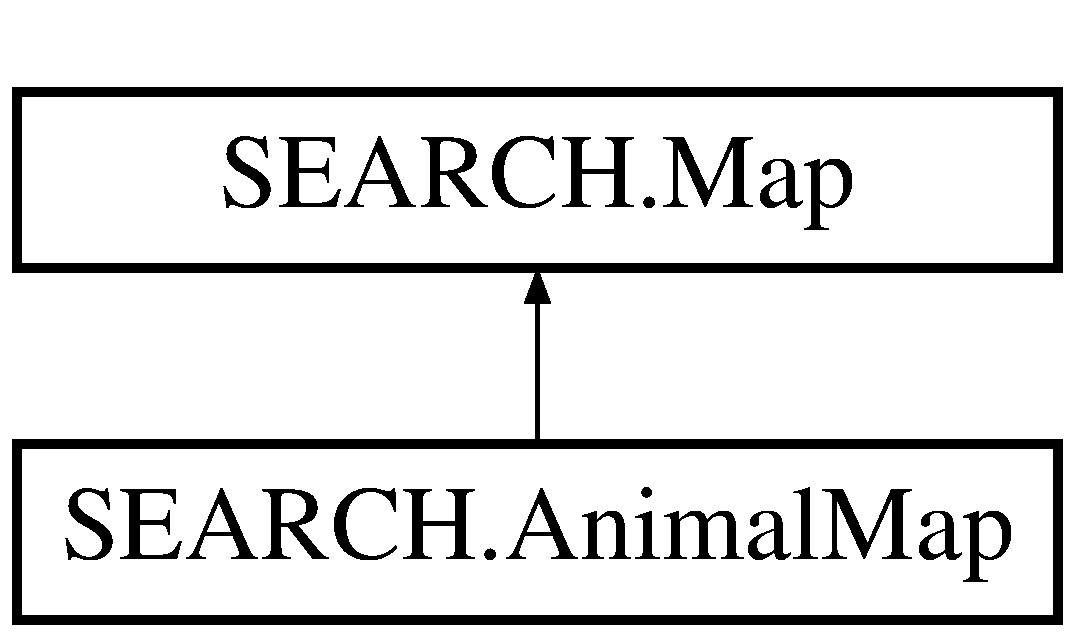
\includegraphics[height=2.000000cm]{class_s_e_a_r_c_h_1_1_animal_map}
\end{center}
\end{figure}
\subsection*{Public Member Functions}
\begin{DoxyCompactItemize}
\item 
\hyperlink{class_s_e_a_r_c_h_1_1_animal_map_a79382e8c9a4e1cbaae3de901e0fd24ed}{Animal\-Map} ()
\item 
\hyperlink{class_s_e_a_r_c_h_1_1_animal_map_aa2dfd4fc4f942d9b299f4d4b8d501608}{Animal\-Map} (string in\-Name, string path, I\-Geometry\-Def in\-Geo\-Def)
\item 
void \hyperlink{class_s_e_a_r_c_h_1_1_animal_map_a6ed6c8c313feec7be632ef0f4697963f}{add\-Polygon} (I\-Polygon in\-Poly)
\item 
void \hyperlink{class_s_e_a_r_c_h_1_1_animal_map_a5b3b4e4765559402ef5404a2c0373e43}{add\-Polygon} (I\-Polygon in\-Poly, int time\-Step)
\item 
void \hyperlink{class_s_e_a_r_c_h_1_1_animal_map_a8f1f2532da51cd312636ac41d8b6b942}{dissolve\-Available\-Polygons} (string in\-Time\-Step, I\-Table input\-Table)
\item 
void \hyperlink{class_s_e_a_r_c_h_1_1_animal_map_a14b7fe17a2637d6f661e2596211a03f4}{explode} (string time\-Step)
\item 
void \hyperlink{class_s_e_a_r_c_h_1_1_animal_map_ac9ec9757b1cd9fa25cdc0e99a8ba3067}{make\-Single\-Part} (string time\-Step)
\item 
I\-Feature\-Class \hyperlink{class_s_e_a_r_c_h_1_1_animal_map_aa4c372afeca550f23febe2d7808ce585}{get\-Shape\-File} (string file\-Name)
\item 
new void \hyperlink{class_s_e_a_r_c_h_1_1_animal_map_a159d6ec5f0db0e5bdc8a40eb762ba824}{remove\-Polygon} (I\-Feature in\-F)
\item 
void \hyperlink{class_s_e_a_r_c_h_1_1_animal_map_a5988e7ac4983a12321f686f7ccccabe2}{reset\-Curr\-Step} ()
\item 
void \hyperlink{class_s_e_a_r_c_h_1_1_animal_map_a9f2eac746c9e56ca7984928f98a5c0aa}{reset\-Base\-Map} ()
\item 
bool \hyperlink{class_s_e_a_r_c_h_1_1_animal_map_a816576e45d5bc17b258be6b527a171ab}{make\-Map} (string shape\-Path, string shape\-File\-Name, I\-Geometry\-Def in\-Geo\-Def)
\item 
I\-Table \hyperlink{class_s_e_a_r_c_h_1_1_animal_map_ae6743d97a2c8a3aaeb54fcfd29b5b9c7}{get\-Union\-Table} ()
\item 
void \hyperlink{class_s_e_a_r_c_h_1_1_animal_map_aadb33fdab6d0078957ea381189a2f001}{remove\-Extra\-Fields} ()
\end{DoxyCompactItemize}
\subsection*{Properties}
\begin{DoxyCompactItemize}
\item 
I\-Table \hyperlink{class_s_e_a_r_c_h_1_1_animal_map_a12649a5f19bffabf46302dc8e1b6f534}{Step\-Table}\hspace{0.3cm}{\ttfamily  \mbox{[}get, set\mbox{]}}
\item 
I\-Feature\-Class \hyperlink{class_s_e_a_r_c_h_1_1_animal_map_a2b6854c8e39aeb885a75cee316ef172b}{Step\-Feature\-Class}\hspace{0.3cm}{\ttfamily  \mbox{[}get, set\mbox{]}}
\item 
I\-Feature\-Class \hyperlink{class_s_e_a_r_c_h_1_1_animal_map_a5a6d17ff0edb0d49d9b687bb9cceadc0}{Suitable\-Feature\-Class}\hspace{0.3cm}{\ttfamily  \mbox{[}get, set\mbox{]}}
\item 
string \hyperlink{class_s_e_a_r_c_h_1_1_animal_map_a3078ba4a94c24d435458cc88d34983a3}{Err\-Message}\hspace{0.3cm}{\ttfamily  \mbox{[}get, set\mbox{]}}
\item 
\hyperlink{class_s_e_a_r_c_h_1_1_map}{Map} \hyperlink{class_s_e_a_r_c_h_1_1_animal_map_a1a2a7f3b8b78337a9e1d8210ae31f71f}{My\-Social\-Map}\hspace{0.3cm}{\ttfamily  \mbox{[}get, set\mbox{]}}
\end{DoxyCompactItemize}
\subsection*{Additional Inherited Members}


\subsection{Detailed Description}
Summary description for \hyperlink{class_s_e_a_r_c_h_1_1_animal_map}{Animal\-Map}. 



\subsection{Constructor \& Destructor Documentation}
\hypertarget{class_s_e_a_r_c_h_1_1_animal_map_a79382e8c9a4e1cbaae3de901e0fd24ed}{\index{S\-E\-A\-R\-C\-H\-::\-Animal\-Map@{S\-E\-A\-R\-C\-H\-::\-Animal\-Map}!Animal\-Map@{Animal\-Map}}
\index{Animal\-Map@{Animal\-Map}!SEARCH::AnimalMap@{S\-E\-A\-R\-C\-H\-::\-Animal\-Map}}
\subsubsection[{Animal\-Map}]{\setlength{\rightskip}{0pt plus 5cm}S\-E\-A\-R\-C\-H.\-Animal\-Map.\-Animal\-Map (
\begin{DoxyParamCaption}
{}
\end{DoxyParamCaption}
)}}\label{class_s_e_a_r_c_h_1_1_animal_map_a79382e8c9a4e1cbaae3de901e0fd24ed}
\hypertarget{class_s_e_a_r_c_h_1_1_animal_map_aa2dfd4fc4f942d9b299f4d4b8d501608}{\index{S\-E\-A\-R\-C\-H\-::\-Animal\-Map@{S\-E\-A\-R\-C\-H\-::\-Animal\-Map}!Animal\-Map@{Animal\-Map}}
\index{Animal\-Map@{Animal\-Map}!SEARCH::AnimalMap@{S\-E\-A\-R\-C\-H\-::\-Animal\-Map}}
\subsubsection[{Animal\-Map}]{\setlength{\rightskip}{0pt plus 5cm}S\-E\-A\-R\-C\-H.\-Animal\-Map.\-Animal\-Map (
\begin{DoxyParamCaption}
\item[{string}]{in\-Name, }
\item[{string}]{path, }
\item[{I\-Geometry\-Def}]{in\-Geo\-Def}
\end{DoxyParamCaption}
)}}\label{class_s_e_a_r_c_h_1_1_animal_map_aa2dfd4fc4f942d9b299f4d4b8d501608}


\subsection{Member Function Documentation}
\hypertarget{class_s_e_a_r_c_h_1_1_animal_map_a6ed6c8c313feec7be632ef0f4697963f}{\index{S\-E\-A\-R\-C\-H\-::\-Animal\-Map@{S\-E\-A\-R\-C\-H\-::\-Animal\-Map}!add\-Polygon@{add\-Polygon}}
\index{add\-Polygon@{add\-Polygon}!SEARCH::AnimalMap@{S\-E\-A\-R\-C\-H\-::\-Animal\-Map}}
\subsubsection[{add\-Polygon}]{\setlength{\rightskip}{0pt plus 5cm}void S\-E\-A\-R\-C\-H.\-Animal\-Map.\-add\-Polygon (
\begin{DoxyParamCaption}
\item[{I\-Polygon}]{in\-Poly}
\end{DoxyParamCaption}
)}}\label{class_s_e_a_r_c_h_1_1_animal_map_a6ed6c8c313feec7be632ef0f4697963f}
\hypertarget{class_s_e_a_r_c_h_1_1_animal_map_a5b3b4e4765559402ef5404a2c0373e43}{\index{S\-E\-A\-R\-C\-H\-::\-Animal\-Map@{S\-E\-A\-R\-C\-H\-::\-Animal\-Map}!add\-Polygon@{add\-Polygon}}
\index{add\-Polygon@{add\-Polygon}!SEARCH::AnimalMap@{S\-E\-A\-R\-C\-H\-::\-Animal\-Map}}
\subsubsection[{add\-Polygon}]{\setlength{\rightskip}{0pt plus 5cm}void S\-E\-A\-R\-C\-H.\-Animal\-Map.\-add\-Polygon (
\begin{DoxyParamCaption}
\item[{I\-Polygon}]{in\-Poly, }
\item[{int}]{time\-Step}
\end{DoxyParamCaption}
)}}\label{class_s_e_a_r_c_h_1_1_animal_map_a5b3b4e4765559402ef5404a2c0373e43}
\hypertarget{class_s_e_a_r_c_h_1_1_animal_map_a8f1f2532da51cd312636ac41d8b6b942}{\index{S\-E\-A\-R\-C\-H\-::\-Animal\-Map@{S\-E\-A\-R\-C\-H\-::\-Animal\-Map}!dissolve\-Available\-Polygons@{dissolve\-Available\-Polygons}}
\index{dissolve\-Available\-Polygons@{dissolve\-Available\-Polygons}!SEARCH::AnimalMap@{S\-E\-A\-R\-C\-H\-::\-Animal\-Map}}
\subsubsection[{dissolve\-Available\-Polygons}]{\setlength{\rightskip}{0pt plus 5cm}void S\-E\-A\-R\-C\-H.\-Animal\-Map.\-dissolve\-Available\-Polygons (
\begin{DoxyParamCaption}
\item[{string}]{in\-Time\-Step, }
\item[{I\-Table}]{input\-Table}
\end{DoxyParamCaption}
)}}\label{class_s_e_a_r_c_h_1_1_animal_map_a8f1f2532da51cd312636ac41d8b6b942}
\hypertarget{class_s_e_a_r_c_h_1_1_animal_map_a14b7fe17a2637d6f661e2596211a03f4}{\index{S\-E\-A\-R\-C\-H\-::\-Animal\-Map@{S\-E\-A\-R\-C\-H\-::\-Animal\-Map}!explode@{explode}}
\index{explode@{explode}!SEARCH::AnimalMap@{S\-E\-A\-R\-C\-H\-::\-Animal\-Map}}
\subsubsection[{explode}]{\setlength{\rightskip}{0pt plus 5cm}void S\-E\-A\-R\-C\-H.\-Animal\-Map.\-explode (
\begin{DoxyParamCaption}
\item[{string}]{time\-Step}
\end{DoxyParamCaption}
)}}\label{class_s_e_a_r_c_h_1_1_animal_map_a14b7fe17a2637d6f661e2596211a03f4}
\hypertarget{class_s_e_a_r_c_h_1_1_animal_map_aa4c372afeca550f23febe2d7808ce585}{\index{S\-E\-A\-R\-C\-H\-::\-Animal\-Map@{S\-E\-A\-R\-C\-H\-::\-Animal\-Map}!get\-Shape\-File@{get\-Shape\-File}}
\index{get\-Shape\-File@{get\-Shape\-File}!SEARCH::AnimalMap@{S\-E\-A\-R\-C\-H\-::\-Animal\-Map}}
\subsubsection[{get\-Shape\-File}]{\setlength{\rightskip}{0pt plus 5cm}I\-Feature\-Class S\-E\-A\-R\-C\-H.\-Animal\-Map.\-get\-Shape\-File (
\begin{DoxyParamCaption}
\item[{string}]{file\-Name}
\end{DoxyParamCaption}
)}}\label{class_s_e_a_r_c_h_1_1_animal_map_aa4c372afeca550f23febe2d7808ce585}
\hypertarget{class_s_e_a_r_c_h_1_1_animal_map_ae6743d97a2c8a3aaeb54fcfd29b5b9c7}{\index{S\-E\-A\-R\-C\-H\-::\-Animal\-Map@{S\-E\-A\-R\-C\-H\-::\-Animal\-Map}!get\-Union\-Table@{get\-Union\-Table}}
\index{get\-Union\-Table@{get\-Union\-Table}!SEARCH::AnimalMap@{S\-E\-A\-R\-C\-H\-::\-Animal\-Map}}
\subsubsection[{get\-Union\-Table}]{\setlength{\rightskip}{0pt plus 5cm}I\-Table S\-E\-A\-R\-C\-H.\-Animal\-Map.\-get\-Union\-Table (
\begin{DoxyParamCaption}
{}
\end{DoxyParamCaption}
)}}\label{class_s_e_a_r_c_h_1_1_animal_map_ae6743d97a2c8a3aaeb54fcfd29b5b9c7}
\hypertarget{class_s_e_a_r_c_h_1_1_animal_map_a816576e45d5bc17b258be6b527a171ab}{\index{S\-E\-A\-R\-C\-H\-::\-Animal\-Map@{S\-E\-A\-R\-C\-H\-::\-Animal\-Map}!make\-Map@{make\-Map}}
\index{make\-Map@{make\-Map}!SEARCH::AnimalMap@{S\-E\-A\-R\-C\-H\-::\-Animal\-Map}}
\subsubsection[{make\-Map}]{\setlength{\rightskip}{0pt plus 5cm}bool S\-E\-A\-R\-C\-H.\-Animal\-Map.\-make\-Map (
\begin{DoxyParamCaption}
\item[{string}]{shape\-Path, }
\item[{string}]{shape\-File\-Name, }
\item[{I\-Geometry\-Def}]{in\-Geo\-Def}
\end{DoxyParamCaption}
)}}\label{class_s_e_a_r_c_h_1_1_animal_map_a816576e45d5bc17b258be6b527a171ab}
\hypertarget{class_s_e_a_r_c_h_1_1_animal_map_ac9ec9757b1cd9fa25cdc0e99a8ba3067}{\index{S\-E\-A\-R\-C\-H\-::\-Animal\-Map@{S\-E\-A\-R\-C\-H\-::\-Animal\-Map}!make\-Single\-Part@{make\-Single\-Part}}
\index{make\-Single\-Part@{make\-Single\-Part}!SEARCH::AnimalMap@{S\-E\-A\-R\-C\-H\-::\-Animal\-Map}}
\subsubsection[{make\-Single\-Part}]{\setlength{\rightskip}{0pt plus 5cm}void S\-E\-A\-R\-C\-H.\-Animal\-Map.\-make\-Single\-Part (
\begin{DoxyParamCaption}
\item[{string}]{time\-Step}
\end{DoxyParamCaption}
)}}\label{class_s_e_a_r_c_h_1_1_animal_map_ac9ec9757b1cd9fa25cdc0e99a8ba3067}
\hypertarget{class_s_e_a_r_c_h_1_1_animal_map_aadb33fdab6d0078957ea381189a2f001}{\index{S\-E\-A\-R\-C\-H\-::\-Animal\-Map@{S\-E\-A\-R\-C\-H\-::\-Animal\-Map}!remove\-Extra\-Fields@{remove\-Extra\-Fields}}
\index{remove\-Extra\-Fields@{remove\-Extra\-Fields}!SEARCH::AnimalMap@{S\-E\-A\-R\-C\-H\-::\-Animal\-Map}}
\subsubsection[{remove\-Extra\-Fields}]{\setlength{\rightskip}{0pt plus 5cm}void S\-E\-A\-R\-C\-H.\-Animal\-Map.\-remove\-Extra\-Fields (
\begin{DoxyParamCaption}
{}
\end{DoxyParamCaption}
)}}\label{class_s_e_a_r_c_h_1_1_animal_map_aadb33fdab6d0078957ea381189a2f001}
\hypertarget{class_s_e_a_r_c_h_1_1_animal_map_a159d6ec5f0db0e5bdc8a40eb762ba824}{\index{S\-E\-A\-R\-C\-H\-::\-Animal\-Map@{S\-E\-A\-R\-C\-H\-::\-Animal\-Map}!remove\-Polygon@{remove\-Polygon}}
\index{remove\-Polygon@{remove\-Polygon}!SEARCH::AnimalMap@{S\-E\-A\-R\-C\-H\-::\-Animal\-Map}}
\subsubsection[{remove\-Polygon}]{\setlength{\rightskip}{0pt plus 5cm}new void S\-E\-A\-R\-C\-H.\-Animal\-Map.\-remove\-Polygon (
\begin{DoxyParamCaption}
\item[{I\-Feature}]{in\-F}
\end{DoxyParamCaption}
)}}\label{class_s_e_a_r_c_h_1_1_animal_map_a159d6ec5f0db0e5bdc8a40eb762ba824}
\hypertarget{class_s_e_a_r_c_h_1_1_animal_map_a9f2eac746c9e56ca7984928f98a5c0aa}{\index{S\-E\-A\-R\-C\-H\-::\-Animal\-Map@{S\-E\-A\-R\-C\-H\-::\-Animal\-Map}!reset\-Base\-Map@{reset\-Base\-Map}}
\index{reset\-Base\-Map@{reset\-Base\-Map}!SEARCH::AnimalMap@{S\-E\-A\-R\-C\-H\-::\-Animal\-Map}}
\subsubsection[{reset\-Base\-Map}]{\setlength{\rightskip}{0pt plus 5cm}void S\-E\-A\-R\-C\-H.\-Animal\-Map.\-reset\-Base\-Map (
\begin{DoxyParamCaption}
{}
\end{DoxyParamCaption}
)}}\label{class_s_e_a_r_c_h_1_1_animal_map_a9f2eac746c9e56ca7984928f98a5c0aa}
\hypertarget{class_s_e_a_r_c_h_1_1_animal_map_a5988e7ac4983a12321f686f7ccccabe2}{\index{S\-E\-A\-R\-C\-H\-::\-Animal\-Map@{S\-E\-A\-R\-C\-H\-::\-Animal\-Map}!reset\-Curr\-Step@{reset\-Curr\-Step}}
\index{reset\-Curr\-Step@{reset\-Curr\-Step}!SEARCH::AnimalMap@{S\-E\-A\-R\-C\-H\-::\-Animal\-Map}}
\subsubsection[{reset\-Curr\-Step}]{\setlength{\rightskip}{0pt plus 5cm}void S\-E\-A\-R\-C\-H.\-Animal\-Map.\-reset\-Curr\-Step (
\begin{DoxyParamCaption}
{}
\end{DoxyParamCaption}
)}}\label{class_s_e_a_r_c_h_1_1_animal_map_a5988e7ac4983a12321f686f7ccccabe2}


\subsection{Property Documentation}
\hypertarget{class_s_e_a_r_c_h_1_1_animal_map_a3078ba4a94c24d435458cc88d34983a3}{\index{S\-E\-A\-R\-C\-H\-::\-Animal\-Map@{S\-E\-A\-R\-C\-H\-::\-Animal\-Map}!Err\-Message@{Err\-Message}}
\index{Err\-Message@{Err\-Message}!SEARCH::AnimalMap@{S\-E\-A\-R\-C\-H\-::\-Animal\-Map}}
\subsubsection[{Err\-Message}]{\setlength{\rightskip}{0pt plus 5cm}string S\-E\-A\-R\-C\-H.\-Animal\-Map.\-Err\-Message\hspace{0.3cm}{\ttfamily [get]}, {\ttfamily [set]}}}\label{class_s_e_a_r_c_h_1_1_animal_map_a3078ba4a94c24d435458cc88d34983a3}
\hypertarget{class_s_e_a_r_c_h_1_1_animal_map_a1a2a7f3b8b78337a9e1d8210ae31f71f}{\index{S\-E\-A\-R\-C\-H\-::\-Animal\-Map@{S\-E\-A\-R\-C\-H\-::\-Animal\-Map}!My\-Social\-Map@{My\-Social\-Map}}
\index{My\-Social\-Map@{My\-Social\-Map}!SEARCH::AnimalMap@{S\-E\-A\-R\-C\-H\-::\-Animal\-Map}}
\subsubsection[{My\-Social\-Map}]{\setlength{\rightskip}{0pt plus 5cm}{\bf Map} S\-E\-A\-R\-C\-H.\-Animal\-Map.\-My\-Social\-Map\hspace{0.3cm}{\ttfamily [get]}, {\ttfamily [set]}}}\label{class_s_e_a_r_c_h_1_1_animal_map_a1a2a7f3b8b78337a9e1d8210ae31f71f}
\hypertarget{class_s_e_a_r_c_h_1_1_animal_map_a2b6854c8e39aeb885a75cee316ef172b}{\index{S\-E\-A\-R\-C\-H\-::\-Animal\-Map@{S\-E\-A\-R\-C\-H\-::\-Animal\-Map}!Step\-Feature\-Class@{Step\-Feature\-Class}}
\index{Step\-Feature\-Class@{Step\-Feature\-Class}!SEARCH::AnimalMap@{S\-E\-A\-R\-C\-H\-::\-Animal\-Map}}
\subsubsection[{Step\-Feature\-Class}]{\setlength{\rightskip}{0pt plus 5cm}I\-Feature\-Class S\-E\-A\-R\-C\-H.\-Animal\-Map.\-Step\-Feature\-Class\hspace{0.3cm}{\ttfamily [get]}, {\ttfamily [set]}}}\label{class_s_e_a_r_c_h_1_1_animal_map_a2b6854c8e39aeb885a75cee316ef172b}
\hypertarget{class_s_e_a_r_c_h_1_1_animal_map_a12649a5f19bffabf46302dc8e1b6f534}{\index{S\-E\-A\-R\-C\-H\-::\-Animal\-Map@{S\-E\-A\-R\-C\-H\-::\-Animal\-Map}!Step\-Table@{Step\-Table}}
\index{Step\-Table@{Step\-Table}!SEARCH::AnimalMap@{S\-E\-A\-R\-C\-H\-::\-Animal\-Map}}
\subsubsection[{Step\-Table}]{\setlength{\rightskip}{0pt plus 5cm}I\-Table S\-E\-A\-R\-C\-H.\-Animal\-Map.\-Step\-Table\hspace{0.3cm}{\ttfamily [get]}, {\ttfamily [set]}}}\label{class_s_e_a_r_c_h_1_1_animal_map_a12649a5f19bffabf46302dc8e1b6f534}
\hypertarget{class_s_e_a_r_c_h_1_1_animal_map_a5a6d17ff0edb0d49d9b687bb9cceadc0}{\index{S\-E\-A\-R\-C\-H\-::\-Animal\-Map@{S\-E\-A\-R\-C\-H\-::\-Animal\-Map}!Suitable\-Feature\-Class@{Suitable\-Feature\-Class}}
\index{Suitable\-Feature\-Class@{Suitable\-Feature\-Class}!SEARCH::AnimalMap@{S\-E\-A\-R\-C\-H\-::\-Animal\-Map}}
\subsubsection[{Suitable\-Feature\-Class}]{\setlength{\rightskip}{0pt plus 5cm}I\-Feature\-Class S\-E\-A\-R\-C\-H.\-Animal\-Map.\-Suitable\-Feature\-Class\hspace{0.3cm}{\ttfamily [get]}, {\ttfamily [set]}}}\label{class_s_e_a_r_c_h_1_1_animal_map_a5a6d17ff0edb0d49d9b687bb9cceadc0}


The documentation for this class was generated from the following file\-:\begin{DoxyCompactItemize}
\item 
Desktop/vlog4net\-A\-R\-C10\-\_\-64\-\_\-newhoming/\-Data\-Centric/\hyperlink{_animal_map_8cs}{Animal\-Map.\-cs}\end{DoxyCompactItemize}

\hypertarget{class_s_e_a_r_c_h_1_1_beam_me_home_scotty_mover}{\section{S\-E\-A\-R\-C\-H.\-Beam\-Me\-Home\-Scotty\-Mover Class Reference}
\label{class_s_e_a_r_c_h_1_1_beam_me_home_scotty_mover}\index{S\-E\-A\-R\-C\-H.\-Beam\-Me\-Home\-Scotty\-Mover@{S\-E\-A\-R\-C\-H.\-Beam\-Me\-Home\-Scotty\-Mover}}
}


Used to move an animal to its home range  


Inheritance diagram for S\-E\-A\-R\-C\-H.\-Beam\-Me\-Home\-Scotty\-Mover\-:\begin{figure}[H]
\begin{center}
\leavevmode
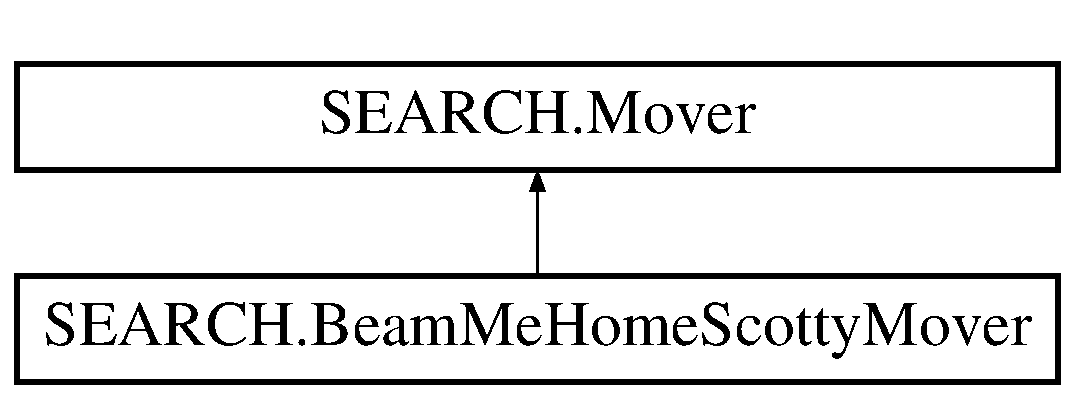
\includegraphics[height=2.000000cm]{class_s_e_a_r_c_h_1_1_beam_me_home_scotty_mover}
\end{center}
\end{figure}
\subsection*{Public Member Functions}
\begin{DoxyCompactItemize}
\item 
\hyperlink{class_s_e_a_r_c_h_1_1_beam_me_home_scotty_mover_a3f982f1b6d6733eef1de5f6fe6b3a6c1}{Beam\-Me\-Home\-Scotty\-Mover} ()
\item 
override double \hyperlink{class_s_e_a_r_c_h_1_1_beam_me_home_scotty_mover_a93c92d2db0bb4df1703a5f4f38c2eb02}{get\-Step\-Length} ()
\item 
override double \hyperlink{class_s_e_a_r_c_h_1_1_beam_me_home_scotty_mover_ae8123c9563cd5149d6ce679fe4b13357}{get\-Turn\-Angle} (double rho)
\item 
override void \hyperlink{class_s_e_a_r_c_h_1_1_beam_me_home_scotty_mover_aae251857ff44aea02591128c50a16e96}{move} (ref double percent\-Time\-Step, \hyperlink{class_s_e_a_r_c_h_1_1_animal}{Animal} in\-A)
\end{DoxyCompactItemize}
\subsection*{Additional Inherited Members}


\subsection{Detailed Description}
Used to move an animal to its home range 



\subsection{Constructor \& Destructor Documentation}
\hypertarget{class_s_e_a_r_c_h_1_1_beam_me_home_scotty_mover_a3f982f1b6d6733eef1de5f6fe6b3a6c1}{\index{S\-E\-A\-R\-C\-H\-::\-Beam\-Me\-Home\-Scotty\-Mover@{S\-E\-A\-R\-C\-H\-::\-Beam\-Me\-Home\-Scotty\-Mover}!Beam\-Me\-Home\-Scotty\-Mover@{Beam\-Me\-Home\-Scotty\-Mover}}
\index{Beam\-Me\-Home\-Scotty\-Mover@{Beam\-Me\-Home\-Scotty\-Mover}!SEARCH::BeamMeHomeScottyMover@{S\-E\-A\-R\-C\-H\-::\-Beam\-Me\-Home\-Scotty\-Mover}}
\subsubsection[{Beam\-Me\-Home\-Scotty\-Mover}]{\setlength{\rightskip}{0pt plus 5cm}S\-E\-A\-R\-C\-H.\-Beam\-Me\-Home\-Scotty\-Mover.\-Beam\-Me\-Home\-Scotty\-Mover (
\begin{DoxyParamCaption}
{}
\end{DoxyParamCaption}
)}}\label{class_s_e_a_r_c_h_1_1_beam_me_home_scotty_mover_a3f982f1b6d6733eef1de5f6fe6b3a6c1}


\subsection{Member Function Documentation}
\hypertarget{class_s_e_a_r_c_h_1_1_beam_me_home_scotty_mover_a93c92d2db0bb4df1703a5f4f38c2eb02}{\index{S\-E\-A\-R\-C\-H\-::\-Beam\-Me\-Home\-Scotty\-Mover@{S\-E\-A\-R\-C\-H\-::\-Beam\-Me\-Home\-Scotty\-Mover}!get\-Step\-Length@{get\-Step\-Length}}
\index{get\-Step\-Length@{get\-Step\-Length}!SEARCH::BeamMeHomeScottyMover@{S\-E\-A\-R\-C\-H\-::\-Beam\-Me\-Home\-Scotty\-Mover}}
\subsubsection[{get\-Step\-Length}]{\setlength{\rightskip}{0pt plus 5cm}override double S\-E\-A\-R\-C\-H.\-Beam\-Me\-Home\-Scotty\-Mover.\-get\-Step\-Length (
\begin{DoxyParamCaption}
{}
\end{DoxyParamCaption}
)\hspace{0.3cm}{\ttfamily [virtual]}}}\label{class_s_e_a_r_c_h_1_1_beam_me_home_scotty_mover_a93c92d2db0bb4df1703a5f4f38c2eb02}


Implements \hyperlink{class_s_e_a_r_c_h_1_1_mover_a3e547800bbc34492f4251adee70dbf02}{S\-E\-A\-R\-C\-H.\-Mover}.

\hypertarget{class_s_e_a_r_c_h_1_1_beam_me_home_scotty_mover_ae8123c9563cd5149d6ce679fe4b13357}{\index{S\-E\-A\-R\-C\-H\-::\-Beam\-Me\-Home\-Scotty\-Mover@{S\-E\-A\-R\-C\-H\-::\-Beam\-Me\-Home\-Scotty\-Mover}!get\-Turn\-Angle@{get\-Turn\-Angle}}
\index{get\-Turn\-Angle@{get\-Turn\-Angle}!SEARCH::BeamMeHomeScottyMover@{S\-E\-A\-R\-C\-H\-::\-Beam\-Me\-Home\-Scotty\-Mover}}
\subsubsection[{get\-Turn\-Angle}]{\setlength{\rightskip}{0pt plus 5cm}override double S\-E\-A\-R\-C\-H.\-Beam\-Me\-Home\-Scotty\-Mover.\-get\-Turn\-Angle (
\begin{DoxyParamCaption}
\item[{double}]{rho}
\end{DoxyParamCaption}
)\hspace{0.3cm}{\ttfamily [virtual]}}}\label{class_s_e_a_r_c_h_1_1_beam_me_home_scotty_mover_ae8123c9563cd5149d6ce679fe4b13357}


Implements \hyperlink{class_s_e_a_r_c_h_1_1_mover_a879a44d5a0c57434375a69c8d8d00e35}{S\-E\-A\-R\-C\-H.\-Mover}.

\hypertarget{class_s_e_a_r_c_h_1_1_beam_me_home_scotty_mover_aae251857ff44aea02591128c50a16e96}{\index{S\-E\-A\-R\-C\-H\-::\-Beam\-Me\-Home\-Scotty\-Mover@{S\-E\-A\-R\-C\-H\-::\-Beam\-Me\-Home\-Scotty\-Mover}!move@{move}}
\index{move@{move}!SEARCH::BeamMeHomeScottyMover@{S\-E\-A\-R\-C\-H\-::\-Beam\-Me\-Home\-Scotty\-Mover}}
\subsubsection[{move}]{\setlength{\rightskip}{0pt plus 5cm}override void S\-E\-A\-R\-C\-H.\-Beam\-Me\-Home\-Scotty\-Mover.\-move (
\begin{DoxyParamCaption}
\item[{ref double}]{percent\-Time\-Step, }
\item[{{\bf Animal}}]{in\-A}
\end{DoxyParamCaption}
)\hspace{0.3cm}{\ttfamily [virtual]}}}\label{class_s_e_a_r_c_h_1_1_beam_me_home_scotty_mover_aae251857ff44aea02591128c50a16e96}


Reimplemented from \hyperlink{class_s_e_a_r_c_h_1_1_mover_ab2dfc659f3817ea48d66ff4d7e464d1d}{S\-E\-A\-R\-C\-H.\-Mover}.



The documentation for this class was generated from the following file\-:\begin{DoxyCompactItemize}
\item 
Desktop/vlog4net\-A\-R\-C10\-\_\-64\-\_\-newhoming/\-Data\-Centric/\hyperlink{_beam_me_home_scotty_mover_8cs}{Beam\-Me\-Home\-Scotty\-Mover.\-cs}\end{DoxyCompactItemize}

\hypertarget{class_s_e_a_r_c_h_1_1_behaviour_modifier}{\section{S\-E\-A\-R\-C\-H.\-Behaviour\-Modifier Class Reference}
\label{class_s_e_a_r_c_h_1_1_behaviour_modifier}\index{S\-E\-A\-R\-C\-H.\-Behaviour\-Modifier@{S\-E\-A\-R\-C\-H.\-Behaviour\-Modifier}}
}


This one will modify the animals behavior under the assumption that the animal feels threatned but very hungry. -\/\-The Singleton defines an Instance operation that lets clients access its unique instance. -\/\-It may be responsible for creating its own unique instance.  


Inheritance diagram for S\-E\-A\-R\-C\-H.\-Behaviour\-Modifier\-:\begin{figure}[H]
\begin{center}
\leavevmode
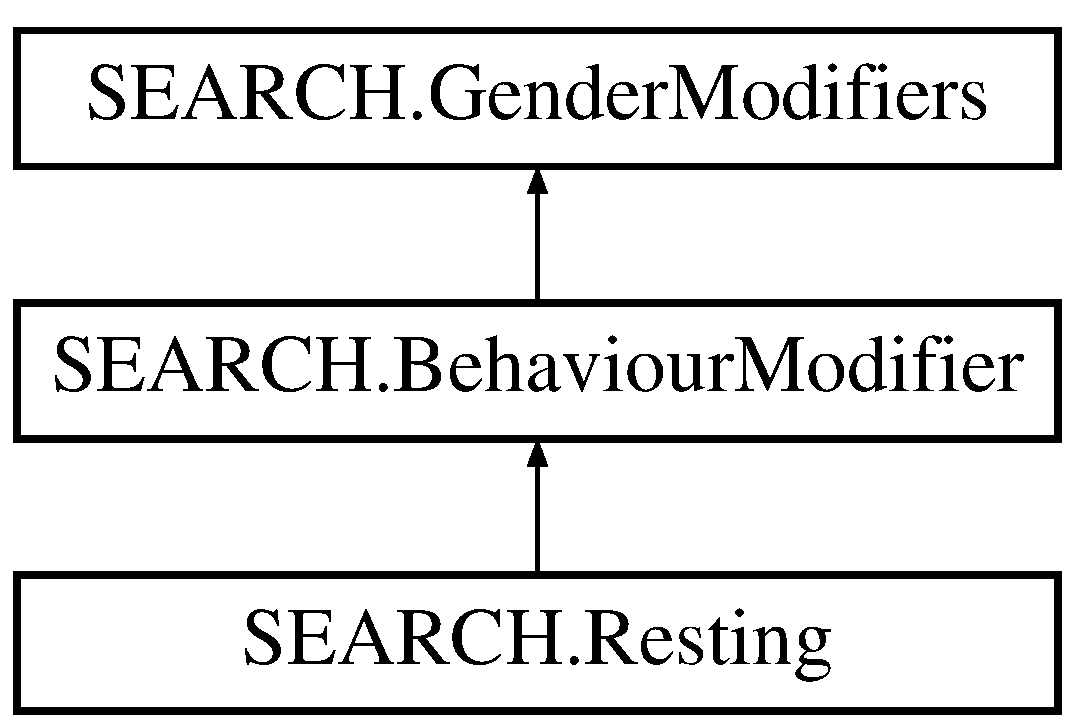
\includegraphics[height=3.000000cm]{class_s_e_a_r_c_h_1_1_behaviour_modifier}
\end{center}
\end{figure}
\subsection*{Static Public Member Functions}
\begin{DoxyCompactItemize}
\item 
static \hyperlink{class_s_e_a_r_c_h_1_1_behaviour_modifier}{Behaviour\-Modifier} \hyperlink{class_s_e_a_r_c_h_1_1_behaviour_modifier_a107e2b884bd8b0e26bacd1a475676147}{Get\-Unique\-Instance} ()
\begin{DoxyCompactList}\small\item\em -\/\-This operation sets the attribute \char`\"{}state\char`\"{} in the Context class. \end{DoxyCompactList}\end{DoxyCompactItemize}
\subsection*{Additional Inherited Members}


\subsection{Detailed Description}
This one will modify the animals behavior under the assumption that the animal feels threatned but very hungry. -\/\-The Singleton defines an Instance operation that lets clients access its unique instance. -\/\-It may be responsible for creating its own unique instance. 

-\/\-The Context defines the interface of interest to clients. -\/\-It maintains an instance of a Concrete\-State subclass that defines the current state.

\subsection{Member Function Documentation}
\hypertarget{class_s_e_a_r_c_h_1_1_behaviour_modifier_a107e2b884bd8b0e26bacd1a475676147}{\index{S\-E\-A\-R\-C\-H\-::\-Behaviour\-Modifier@{S\-E\-A\-R\-C\-H\-::\-Behaviour\-Modifier}!Get\-Unique\-Instance@{Get\-Unique\-Instance}}
\index{Get\-Unique\-Instance@{Get\-Unique\-Instance}!SEARCH::BehaviourModifier@{S\-E\-A\-R\-C\-H\-::\-Behaviour\-Modifier}}
\subsubsection[{Get\-Unique\-Instance}]{\setlength{\rightskip}{0pt plus 5cm}static {\bf Behaviour\-Modifier} S\-E\-A\-R\-C\-H.\-Behaviour\-Modifier.\-Get\-Unique\-Instance (
\begin{DoxyParamCaption}
{}
\end{DoxyParamCaption}
)\hspace{0.3cm}{\ttfamily [static]}}}\label{class_s_e_a_r_c_h_1_1_behaviour_modifier_a107e2b884bd8b0e26bacd1a475676147}


-\/\-This operation sets the attribute \char`\"{}state\char`\"{} in the Context class. 

-\/\-This operation implements the logic for returning the unique instance of the Singleton pattern. 

The documentation for this class was generated from the following file\-:\begin{DoxyCompactItemize}
\item 
Desktop/vlog4net\-A\-R\-C10\-\_\-64\-\_\-newhoming/\-Data\-Centric/\hyperlink{_behavior_modifier_8cs}{Behavior\-Modifier.\-cs}\end{DoxyCompactItemize}

\hypertarget{class_s_e_a_r_c_h_1_1_best_combo_home_range_finder}{\section{S\-E\-A\-R\-C\-H.\-Best\-Combo\-Home\-Range\-Finder Class Reference}
\label{class_s_e_a_r_c_h_1_1_best_combo_home_range_finder}\index{S\-E\-A\-R\-C\-H.\-Best\-Combo\-Home\-Range\-Finder@{S\-E\-A\-R\-C\-H.\-Best\-Combo\-Home\-Range\-Finder}}
}


 


Inheritance diagram for S\-E\-A\-R\-C\-H.\-Best\-Combo\-Home\-Range\-Finder\-:\begin{figure}[H]
\begin{center}
\leavevmode
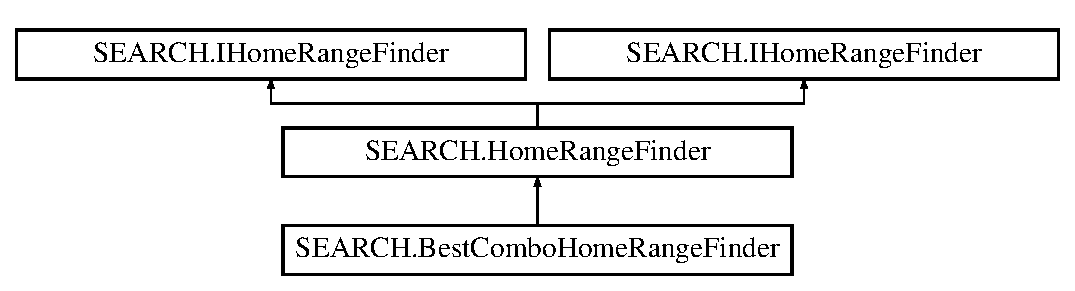
\includegraphics[height=3.000000cm]{class_s_e_a_r_c_h_1_1_best_combo_home_range_finder}
\end{center}
\end{figure}
\subsection*{Public Member Functions}
\begin{DoxyCompactItemize}
\item 
\hyperlink{class_s_e_a_r_c_h_1_1_best_combo_home_range_finder_a4869a6b145a31c5e9ce29d069fe864c9}{Best\-Combo\-Home\-Range\-Finder} ()
\item 
override bool \hyperlink{class_s_e_a_r_c_h_1_1_best_combo_home_range_finder_a3ea0071e375fca09e9116bf627e205b5}{set\-Home\-Range\-Center} (\hyperlink{class_s_e_a_r_c_h_1_1_animal}{Animal} in\-Animal, string in\-File\-Name)
\end{DoxyCompactItemize}
\subsection*{Static Public Member Functions}
\begin{DoxyCompactItemize}
\item 
static \hyperlink{class_s_e_a_r_c_h_1_1_best_combo_home_range_finder}{Best\-Combo\-Home\-Range\-Finder} \hyperlink{class_s_e_a_r_c_h_1_1_best_combo_home_range_finder_a015cb41e11c2ea98733f0d1b1be1dc70}{get\-Instance} ()
\end{DoxyCompactItemize}
\subsection*{Additional Inherited Members}


\subsection{Detailed Description}




\subsection{Constructor \& Destructor Documentation}
\hypertarget{class_s_e_a_r_c_h_1_1_best_combo_home_range_finder_a4869a6b145a31c5e9ce29d069fe864c9}{\index{S\-E\-A\-R\-C\-H\-::\-Best\-Combo\-Home\-Range\-Finder@{S\-E\-A\-R\-C\-H\-::\-Best\-Combo\-Home\-Range\-Finder}!Best\-Combo\-Home\-Range\-Finder@{Best\-Combo\-Home\-Range\-Finder}}
\index{Best\-Combo\-Home\-Range\-Finder@{Best\-Combo\-Home\-Range\-Finder}!SEARCH::BestComboHomeRangeFinder@{S\-E\-A\-R\-C\-H\-::\-Best\-Combo\-Home\-Range\-Finder}}
\subsubsection[{Best\-Combo\-Home\-Range\-Finder}]{\setlength{\rightskip}{0pt plus 5cm}S\-E\-A\-R\-C\-H.\-Best\-Combo\-Home\-Range\-Finder.\-Best\-Combo\-Home\-Range\-Finder (
\begin{DoxyParamCaption}
{}
\end{DoxyParamCaption}
)}}\label{class_s_e_a_r_c_h_1_1_best_combo_home_range_finder_a4869a6b145a31c5e9ce29d069fe864c9}


\subsection{Member Function Documentation}
\hypertarget{class_s_e_a_r_c_h_1_1_best_combo_home_range_finder_a015cb41e11c2ea98733f0d1b1be1dc70}{\index{S\-E\-A\-R\-C\-H\-::\-Best\-Combo\-Home\-Range\-Finder@{S\-E\-A\-R\-C\-H\-::\-Best\-Combo\-Home\-Range\-Finder}!get\-Instance@{get\-Instance}}
\index{get\-Instance@{get\-Instance}!SEARCH::BestComboHomeRangeFinder@{S\-E\-A\-R\-C\-H\-::\-Best\-Combo\-Home\-Range\-Finder}}
\subsubsection[{get\-Instance}]{\setlength{\rightskip}{0pt plus 5cm}static {\bf Best\-Combo\-Home\-Range\-Finder} S\-E\-A\-R\-C\-H.\-Best\-Combo\-Home\-Range\-Finder.\-get\-Instance (
\begin{DoxyParamCaption}
{}
\end{DoxyParamCaption}
)\hspace{0.3cm}{\ttfamily [static]}}}\label{class_s_e_a_r_c_h_1_1_best_combo_home_range_finder_a015cb41e11c2ea98733f0d1b1be1dc70}
\hypertarget{class_s_e_a_r_c_h_1_1_best_combo_home_range_finder_a3ea0071e375fca09e9116bf627e205b5}{\index{S\-E\-A\-R\-C\-H\-::\-Best\-Combo\-Home\-Range\-Finder@{S\-E\-A\-R\-C\-H\-::\-Best\-Combo\-Home\-Range\-Finder}!set\-Home\-Range\-Center@{set\-Home\-Range\-Center}}
\index{set\-Home\-Range\-Center@{set\-Home\-Range\-Center}!SEARCH::BestComboHomeRangeFinder@{S\-E\-A\-R\-C\-H\-::\-Best\-Combo\-Home\-Range\-Finder}}
\subsubsection[{set\-Home\-Range\-Center}]{\setlength{\rightskip}{0pt plus 5cm}override bool S\-E\-A\-R\-C\-H.\-Best\-Combo\-Home\-Range\-Finder.\-set\-Home\-Range\-Center (
\begin{DoxyParamCaption}
\item[{{\bf Animal}}]{in\-Animal, }
\item[{string}]{in\-File\-Name}
\end{DoxyParamCaption}
)\hspace{0.3cm}{\ttfamily [virtual]}}}\label{class_s_e_a_r_c_h_1_1_best_combo_home_range_finder_a3ea0071e375fca09e9116bf627e205b5}


Reimplemented from \hyperlink{class_s_e_a_r_c_h_1_1_home_range_finder_a41b187329b1cd89b91c9c2f4a145ec7b}{S\-E\-A\-R\-C\-H.\-Home\-Range\-Finder}.



The documentation for this class was generated from the following file\-:\begin{DoxyCompactItemize}
\item 
Desktop/vlog4net\-A\-R\-C10\-\_\-64\-\_\-newhoming/\-Data\-Centric/\hyperlink{_best_combo_home_range_finder_8cs}{Best\-Combo\-Home\-Range\-Finder.\-cs}\end{DoxyCompactItemize}

\hypertarget{class_s_e_a_r_c_h_1_1_best_food_home_range_finder}{\section{S\-E\-A\-R\-C\-H.\-Best\-Food\-Home\-Range\-Finder Class Reference}
\label{class_s_e_a_r_c_h_1_1_best_food_home_range_finder}\index{S\-E\-A\-R\-C\-H.\-Best\-Food\-Home\-Range\-Finder@{S\-E\-A\-R\-C\-H.\-Best\-Food\-Home\-Range\-Finder}}
}


Summary description for \hyperlink{class_s_e_a_r_c_h_1_1_best_food_home_range_finder}{Best\-Food\-Home\-Range\-Finder}.  


Inheritance diagram for S\-E\-A\-R\-C\-H.\-Best\-Food\-Home\-Range\-Finder\-:\begin{figure}[H]
\begin{center}
\leavevmode
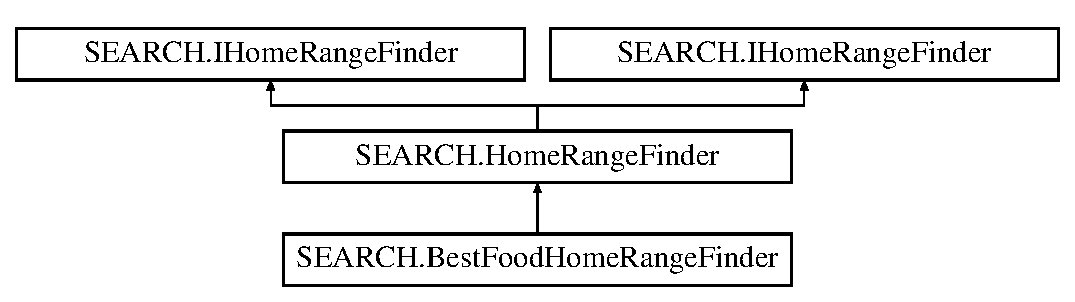
\includegraphics[height=3.000000cm]{class_s_e_a_r_c_h_1_1_best_food_home_range_finder}
\end{center}
\end{figure}
\subsection*{Public Member Functions}
\begin{DoxyCompactItemize}
\item 
\hyperlink{class_s_e_a_r_c_h_1_1_best_food_home_range_finder_aafefcd8a92bb988b9a1f4be2295089ec}{Best\-Food\-Home\-Range\-Finder} ()
\item 
override bool \hyperlink{class_s_e_a_r_c_h_1_1_best_food_home_range_finder_aa9876f866a2bc8ffca635caafb20add3}{set\-Home\-Range\-Center} (\hyperlink{class_s_e_a_r_c_h_1_1_animal}{Animal} in\-Animal, string in\-File\-Name)
\end{DoxyCompactItemize}
\subsection*{Static Public Member Functions}
\begin{DoxyCompactItemize}
\item 
static \hyperlink{class_s_e_a_r_c_h_1_1_best_food_home_range_finder}{Best\-Food\-Home\-Range\-Finder} \hyperlink{class_s_e_a_r_c_h_1_1_best_food_home_range_finder_a4fba25395fd682c52dfceb20a1944309}{get\-Instance} ()
\end{DoxyCompactItemize}
\subsection*{Additional Inherited Members}


\subsection{Detailed Description}
Summary description for \hyperlink{class_s_e_a_r_c_h_1_1_best_food_home_range_finder}{Best\-Food\-Home\-Range\-Finder}. 



\subsection{Constructor \& Destructor Documentation}
\hypertarget{class_s_e_a_r_c_h_1_1_best_food_home_range_finder_aafefcd8a92bb988b9a1f4be2295089ec}{\index{S\-E\-A\-R\-C\-H\-::\-Best\-Food\-Home\-Range\-Finder@{S\-E\-A\-R\-C\-H\-::\-Best\-Food\-Home\-Range\-Finder}!Best\-Food\-Home\-Range\-Finder@{Best\-Food\-Home\-Range\-Finder}}
\index{Best\-Food\-Home\-Range\-Finder@{Best\-Food\-Home\-Range\-Finder}!SEARCH::BestFoodHomeRangeFinder@{S\-E\-A\-R\-C\-H\-::\-Best\-Food\-Home\-Range\-Finder}}
\subsubsection[{Best\-Food\-Home\-Range\-Finder}]{\setlength{\rightskip}{0pt plus 5cm}S\-E\-A\-R\-C\-H.\-Best\-Food\-Home\-Range\-Finder.\-Best\-Food\-Home\-Range\-Finder (
\begin{DoxyParamCaption}
{}
\end{DoxyParamCaption}
)}}\label{class_s_e_a_r_c_h_1_1_best_food_home_range_finder_aafefcd8a92bb988b9a1f4be2295089ec}


\subsection{Member Function Documentation}
\hypertarget{class_s_e_a_r_c_h_1_1_best_food_home_range_finder_a4fba25395fd682c52dfceb20a1944309}{\index{S\-E\-A\-R\-C\-H\-::\-Best\-Food\-Home\-Range\-Finder@{S\-E\-A\-R\-C\-H\-::\-Best\-Food\-Home\-Range\-Finder}!get\-Instance@{get\-Instance}}
\index{get\-Instance@{get\-Instance}!SEARCH::BestFoodHomeRangeFinder@{S\-E\-A\-R\-C\-H\-::\-Best\-Food\-Home\-Range\-Finder}}
\subsubsection[{get\-Instance}]{\setlength{\rightskip}{0pt plus 5cm}static {\bf Best\-Food\-Home\-Range\-Finder} S\-E\-A\-R\-C\-H.\-Best\-Food\-Home\-Range\-Finder.\-get\-Instance (
\begin{DoxyParamCaption}
{}
\end{DoxyParamCaption}
)\hspace{0.3cm}{\ttfamily [static]}}}\label{class_s_e_a_r_c_h_1_1_best_food_home_range_finder_a4fba25395fd682c52dfceb20a1944309}
\hypertarget{class_s_e_a_r_c_h_1_1_best_food_home_range_finder_aa9876f866a2bc8ffca635caafb20add3}{\index{S\-E\-A\-R\-C\-H\-::\-Best\-Food\-Home\-Range\-Finder@{S\-E\-A\-R\-C\-H\-::\-Best\-Food\-Home\-Range\-Finder}!set\-Home\-Range\-Center@{set\-Home\-Range\-Center}}
\index{set\-Home\-Range\-Center@{set\-Home\-Range\-Center}!SEARCH::BestFoodHomeRangeFinder@{S\-E\-A\-R\-C\-H\-::\-Best\-Food\-Home\-Range\-Finder}}
\subsubsection[{set\-Home\-Range\-Center}]{\setlength{\rightskip}{0pt plus 5cm}override bool S\-E\-A\-R\-C\-H.\-Best\-Food\-Home\-Range\-Finder.\-set\-Home\-Range\-Center (
\begin{DoxyParamCaption}
\item[{{\bf Animal}}]{in\-Animal, }
\item[{string}]{in\-File\-Name}
\end{DoxyParamCaption}
)\hspace{0.3cm}{\ttfamily [virtual]}}}\label{class_s_e_a_r_c_h_1_1_best_food_home_range_finder_aa9876f866a2bc8ffca635caafb20add3}


Reimplemented from \hyperlink{class_s_e_a_r_c_h_1_1_home_range_finder_a41b187329b1cd89b91c9c2f4a145ec7b}{S\-E\-A\-R\-C\-H.\-Home\-Range\-Finder}.



The documentation for this class was generated from the following file\-:\begin{DoxyCompactItemize}
\item 
Desktop/vlog4net\-A\-R\-C10\-\_\-64\-\_\-newhoming/\-Data\-Centric/\hyperlink{_best_food_home_range_finder_8cs}{Best\-Food\-Home\-Range\-Finder.\-cs}\end{DoxyCompactItemize}

\hypertarget{class_s_e_a_r_c_h_1_1_best_risk_home_range_finder}{\section{S\-E\-A\-R\-C\-H.\-Best\-Risk\-Home\-Range\-Finder Class Reference}
\label{class_s_e_a_r_c_h_1_1_best_risk_home_range_finder}\index{S\-E\-A\-R\-C\-H.\-Best\-Risk\-Home\-Range\-Finder@{S\-E\-A\-R\-C\-H.\-Best\-Risk\-Home\-Range\-Finder}}
}


 


Inheritance diagram for S\-E\-A\-R\-C\-H.\-Best\-Risk\-Home\-Range\-Finder\-:\begin{figure}[H]
\begin{center}
\leavevmode
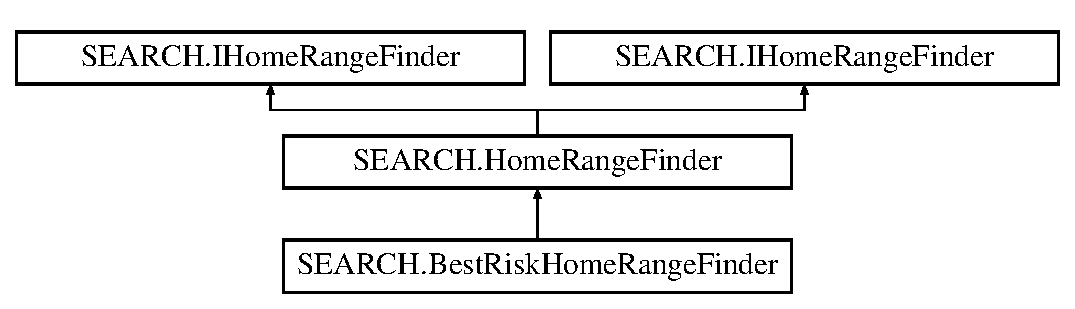
\includegraphics[height=3.000000cm]{class_s_e_a_r_c_h_1_1_best_risk_home_range_finder}
\end{center}
\end{figure}
\subsection*{Public Member Functions}
\begin{DoxyCompactItemize}
\item 
\hyperlink{class_s_e_a_r_c_h_1_1_best_risk_home_range_finder_af55769ce11dc9fd833dcab8c152bd47f}{Best\-Risk\-Home\-Range\-Finder} ()
\item 
override bool \hyperlink{class_s_e_a_r_c_h_1_1_best_risk_home_range_finder_a90867156ad508254624d441fb9116d65}{set\-Home\-Range\-Center} (\hyperlink{class_s_e_a_r_c_h_1_1_animal}{Animal} in\-Animal, string in\-File\-Name)
\end{DoxyCompactItemize}
\subsection*{Static Public Member Functions}
\begin{DoxyCompactItemize}
\item 
static \hyperlink{class_s_e_a_r_c_h_1_1_best_risk_home_range_finder}{Best\-Risk\-Home\-Range\-Finder} \hyperlink{class_s_e_a_r_c_h_1_1_best_risk_home_range_finder_a1f6df4f3d21ccae467fd4335661da4ae}{get\-Instance} ()
\end{DoxyCompactItemize}
\subsection*{Additional Inherited Members}


\subsection{Detailed Description}




\subsection{Constructor \& Destructor Documentation}
\hypertarget{class_s_e_a_r_c_h_1_1_best_risk_home_range_finder_af55769ce11dc9fd833dcab8c152bd47f}{\index{S\-E\-A\-R\-C\-H\-::\-Best\-Risk\-Home\-Range\-Finder@{S\-E\-A\-R\-C\-H\-::\-Best\-Risk\-Home\-Range\-Finder}!Best\-Risk\-Home\-Range\-Finder@{Best\-Risk\-Home\-Range\-Finder}}
\index{Best\-Risk\-Home\-Range\-Finder@{Best\-Risk\-Home\-Range\-Finder}!SEARCH::BestRiskHomeRangeFinder@{S\-E\-A\-R\-C\-H\-::\-Best\-Risk\-Home\-Range\-Finder}}
\subsubsection[{Best\-Risk\-Home\-Range\-Finder}]{\setlength{\rightskip}{0pt plus 5cm}S\-E\-A\-R\-C\-H.\-Best\-Risk\-Home\-Range\-Finder.\-Best\-Risk\-Home\-Range\-Finder (
\begin{DoxyParamCaption}
{}
\end{DoxyParamCaption}
)}}\label{class_s_e_a_r_c_h_1_1_best_risk_home_range_finder_af55769ce11dc9fd833dcab8c152bd47f}


\subsection{Member Function Documentation}
\hypertarget{class_s_e_a_r_c_h_1_1_best_risk_home_range_finder_a1f6df4f3d21ccae467fd4335661da4ae}{\index{S\-E\-A\-R\-C\-H\-::\-Best\-Risk\-Home\-Range\-Finder@{S\-E\-A\-R\-C\-H\-::\-Best\-Risk\-Home\-Range\-Finder}!get\-Instance@{get\-Instance}}
\index{get\-Instance@{get\-Instance}!SEARCH::BestRiskHomeRangeFinder@{S\-E\-A\-R\-C\-H\-::\-Best\-Risk\-Home\-Range\-Finder}}
\subsubsection[{get\-Instance}]{\setlength{\rightskip}{0pt plus 5cm}static {\bf Best\-Risk\-Home\-Range\-Finder} S\-E\-A\-R\-C\-H.\-Best\-Risk\-Home\-Range\-Finder.\-get\-Instance (
\begin{DoxyParamCaption}
{}
\end{DoxyParamCaption}
)\hspace{0.3cm}{\ttfamily [static]}}}\label{class_s_e_a_r_c_h_1_1_best_risk_home_range_finder_a1f6df4f3d21ccae467fd4335661da4ae}
\hypertarget{class_s_e_a_r_c_h_1_1_best_risk_home_range_finder_a90867156ad508254624d441fb9116d65}{\index{S\-E\-A\-R\-C\-H\-::\-Best\-Risk\-Home\-Range\-Finder@{S\-E\-A\-R\-C\-H\-::\-Best\-Risk\-Home\-Range\-Finder}!set\-Home\-Range\-Center@{set\-Home\-Range\-Center}}
\index{set\-Home\-Range\-Center@{set\-Home\-Range\-Center}!SEARCH::BestRiskHomeRangeFinder@{S\-E\-A\-R\-C\-H\-::\-Best\-Risk\-Home\-Range\-Finder}}
\subsubsection[{set\-Home\-Range\-Center}]{\setlength{\rightskip}{0pt plus 5cm}override bool S\-E\-A\-R\-C\-H.\-Best\-Risk\-Home\-Range\-Finder.\-set\-Home\-Range\-Center (
\begin{DoxyParamCaption}
\item[{{\bf Animal}}]{in\-Animal, }
\item[{string}]{in\-File\-Name}
\end{DoxyParamCaption}
)\hspace{0.3cm}{\ttfamily [virtual]}}}\label{class_s_e_a_r_c_h_1_1_best_risk_home_range_finder_a90867156ad508254624d441fb9116d65}


Reimplemented from \hyperlink{class_s_e_a_r_c_h_1_1_home_range_finder_a41b187329b1cd89b91c9c2f4a145ec7b}{S\-E\-A\-R\-C\-H.\-Home\-Range\-Finder}.



The documentation for this class was generated from the following file\-:\begin{DoxyCompactItemize}
\item 
Desktop/vlog4net\-A\-R\-C10\-\_\-64\-\_\-newhoming/\-Data\-Centric/\hyperlink{_best_risk_home_range_finder_8cs}{Best\-Risk\-Home\-Range\-Finder.\-cs}\end{DoxyCompactItemize}

\hypertarget{class_s_e_a_r_c_h_1_1_closest_home_range_finder}{\section{S\-E\-A\-R\-C\-H.\-Closest\-Home\-Range\-Finder Class Reference}
\label{class_s_e_a_r_c_h_1_1_closest_home_range_finder}\index{S\-E\-A\-R\-C\-H.\-Closest\-Home\-Range\-Finder@{S\-E\-A\-R\-C\-H.\-Closest\-Home\-Range\-Finder}}
}


Summary description for \hyperlink{class_s_e_a_r_c_h_1_1_closest_home_range_finder}{Closest\-Home\-Range\-Finder}.  


Inheritance diagram for S\-E\-A\-R\-C\-H.\-Closest\-Home\-Range\-Finder\-:\begin{figure}[H]
\begin{center}
\leavevmode
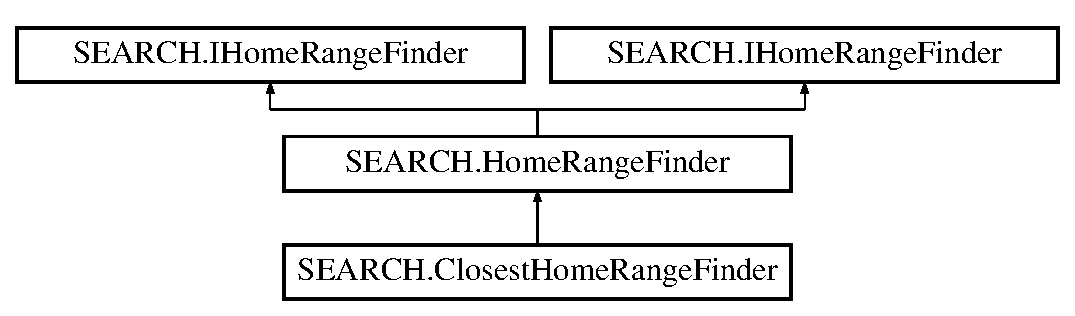
\includegraphics[height=3.000000cm]{class_s_e_a_r_c_h_1_1_closest_home_range_finder}
\end{center}
\end{figure}
\subsection*{Public Member Functions}
\begin{DoxyCompactItemize}
\item 
override bool \hyperlink{class_s_e_a_r_c_h_1_1_closest_home_range_finder_a9f4b1aae4a27e1109c03ea444fdaf185}{set\-Home\-Range\-Center} (\hyperlink{class_s_e_a_r_c_h_1_1_animal}{Animal} in\-Animal, string file\-Name)
\end{DoxyCompactItemize}
\subsection*{Static Public Member Functions}
\begin{DoxyCompactItemize}
\item 
static \hyperlink{class_s_e_a_r_c_h_1_1_closest_home_range_finder}{Closest\-Home\-Range\-Finder} \hyperlink{class_s_e_a_r_c_h_1_1_closest_home_range_finder_a4c409e9d17edbf2855372390bdd1a4a1}{get\-Instance} ()
\end{DoxyCompactItemize}
\subsection*{Additional Inherited Members}


\subsection{Detailed Description}
Summary description for \hyperlink{class_s_e_a_r_c_h_1_1_closest_home_range_finder}{Closest\-Home\-Range\-Finder}. 



\subsection{Member Function Documentation}
\hypertarget{class_s_e_a_r_c_h_1_1_closest_home_range_finder_a4c409e9d17edbf2855372390bdd1a4a1}{\index{S\-E\-A\-R\-C\-H\-::\-Closest\-Home\-Range\-Finder@{S\-E\-A\-R\-C\-H\-::\-Closest\-Home\-Range\-Finder}!get\-Instance@{get\-Instance}}
\index{get\-Instance@{get\-Instance}!SEARCH::ClosestHomeRangeFinder@{S\-E\-A\-R\-C\-H\-::\-Closest\-Home\-Range\-Finder}}
\subsubsection[{get\-Instance}]{\setlength{\rightskip}{0pt plus 5cm}static {\bf Closest\-Home\-Range\-Finder} S\-E\-A\-R\-C\-H.\-Closest\-Home\-Range\-Finder.\-get\-Instance (
\begin{DoxyParamCaption}
{}
\end{DoxyParamCaption}
)\hspace{0.3cm}{\ttfamily [static]}}}\label{class_s_e_a_r_c_h_1_1_closest_home_range_finder_a4c409e9d17edbf2855372390bdd1a4a1}
\hypertarget{class_s_e_a_r_c_h_1_1_closest_home_range_finder_a9f4b1aae4a27e1109c03ea444fdaf185}{\index{S\-E\-A\-R\-C\-H\-::\-Closest\-Home\-Range\-Finder@{S\-E\-A\-R\-C\-H\-::\-Closest\-Home\-Range\-Finder}!set\-Home\-Range\-Center@{set\-Home\-Range\-Center}}
\index{set\-Home\-Range\-Center@{set\-Home\-Range\-Center}!SEARCH::ClosestHomeRangeFinder@{S\-E\-A\-R\-C\-H\-::\-Closest\-Home\-Range\-Finder}}
\subsubsection[{set\-Home\-Range\-Center}]{\setlength{\rightskip}{0pt plus 5cm}override bool S\-E\-A\-R\-C\-H.\-Closest\-Home\-Range\-Finder.\-set\-Home\-Range\-Center (
\begin{DoxyParamCaption}
\item[{{\bf Animal}}]{in\-Animal, }
\item[{string}]{file\-Name}
\end{DoxyParamCaption}
)\hspace{0.3cm}{\ttfamily [virtual]}}}\label{class_s_e_a_r_c_h_1_1_closest_home_range_finder_a9f4b1aae4a27e1109c03ea444fdaf185}


Reimplemented from \hyperlink{class_s_e_a_r_c_h_1_1_home_range_finder_a41b187329b1cd89b91c9c2f4a145ec7b}{S\-E\-A\-R\-C\-H.\-Home\-Range\-Finder}.



The documentation for this class was generated from the following file\-:\begin{DoxyCompactItemize}
\item 
Desktop/vlog4net\-A\-R\-C10\-\_\-64\-\_\-newhoming/\-Data\-Centric/\hyperlink{_closest_home_range_finder_8cs}{Closest\-Home\-Range\-Finder.\-cs}\end{DoxyCompactItemize}

\hypertarget{class_s_e_a_r_c_h_1_1_compare_by_location}{\section{S\-E\-A\-R\-C\-H.\-Compare\-By\-Location Class Reference}
\label{class_s_e_a_r_c_h_1_1_compare_by_location}\index{S\-E\-A\-R\-C\-H.\-Compare\-By\-Location@{S\-E\-A\-R\-C\-H.\-Compare\-By\-Location}}
}
Inheritance diagram for S\-E\-A\-R\-C\-H.\-Compare\-By\-Location\-:\begin{figure}[H]
\begin{center}
\leavevmode
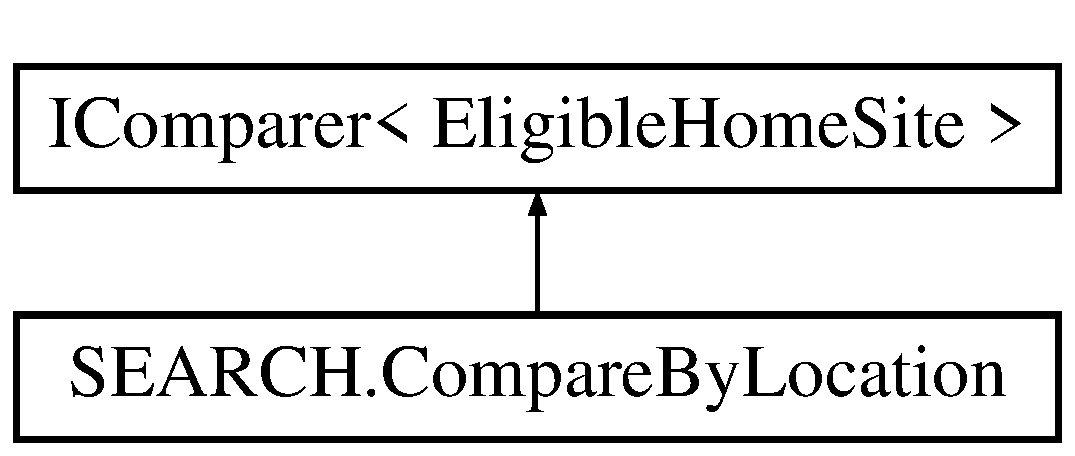
\includegraphics[height=2.000000cm]{class_s_e_a_r_c_h_1_1_compare_by_location}
\end{center}
\end{figure}
\subsection*{Public Member Functions}
\begin{DoxyCompactItemize}
\item 
int \hyperlink{class_s_e_a_r_c_h_1_1_compare_by_location_a6cfd274b9662e9b7aa25225983903240}{Compare} (\hyperlink{class_s_e_a_r_c_h_1_1_eligible_home_site}{Eligible\-Home\-Site} x, \hyperlink{class_s_e_a_r_c_h_1_1_eligible_home_site}{Eligible\-Home\-Site} y)
\end{DoxyCompactItemize}


\subsection{Member Function Documentation}
\hypertarget{class_s_e_a_r_c_h_1_1_compare_by_location_a6cfd274b9662e9b7aa25225983903240}{\index{S\-E\-A\-R\-C\-H\-::\-Compare\-By\-Location@{S\-E\-A\-R\-C\-H\-::\-Compare\-By\-Location}!Compare@{Compare}}
\index{Compare@{Compare}!SEARCH::CompareByLocation@{S\-E\-A\-R\-C\-H\-::\-Compare\-By\-Location}}
\subsubsection[{Compare}]{\setlength{\rightskip}{0pt plus 5cm}int S\-E\-A\-R\-C\-H.\-Compare\-By\-Location.\-Compare (
\begin{DoxyParamCaption}
\item[{{\bf Eligible\-Home\-Site}}]{x, }
\item[{{\bf Eligible\-Home\-Site}}]{y}
\end{DoxyParamCaption}
)}}\label{class_s_e_a_r_c_h_1_1_compare_by_location_a6cfd274b9662e9b7aa25225983903240}


The documentation for this class was generated from the following file\-:\begin{DoxyCompactItemize}
\item 
Desktop/vlog4net\-A\-R\-C10\-\_\-64\-\_\-newhoming/\-Data\-Centric/\hyperlink{_eligible_home_site_8cs}{Eligible\-Home\-Site.\-cs}\end{DoxyCompactItemize}

\hypertarget{class_s_e_a_r_c_h_1_1cross_over_info}{\section{S\-E\-A\-R\-C\-H.\-cross\-Over\-Info Class Reference}
\label{class_s_e_a_r_c_h_1_1cross_over_info}\index{S\-E\-A\-R\-C\-H.\-cross\-Over\-Info@{S\-E\-A\-R\-C\-H.\-cross\-Over\-Info}}
}
\subsection*{Public Member Functions}
\begin{DoxyCompactItemize}
\item 
\hyperlink{class_s_e_a_r_c_h_1_1cross_over_info_afa43185dee09a430129ba8ad43a9b855}{cross\-Over\-Info} ()
\end{DoxyCompactItemize}
\subsection*{Properties}
\begin{DoxyCompactItemize}
\item 
bool \hyperlink{class_s_e_a_r_c_h_1_1cross_over_info_a75324466c49acbc64bb59ee876713f4b}{Changed\-Polys}\hspace{0.3cm}{\ttfamily  \mbox{[}get, set\mbox{]}}
\item 
double \hyperlink{class_s_e_a_r_c_h_1_1cross_over_info_af63c71e631a1f35983a06bb4c798ee05}{Curr\-Poly\-Value}\hspace{0.3cm}{\ttfamily  \mbox{[}get, set\mbox{]}}
\item 
double \hyperlink{class_s_e_a_r_c_h_1_1cross_over_info_a3b72957ce0e0320b86ad7f7b6271be6f}{Distance}\hspace{0.3cm}{\ttfamily  \mbox{[}get, set\mbox{]}}
\item 
Point\-Class \hyperlink{class_s_e_a_r_c_h_1_1cross_over_info_ab0bf18150222aa6504fbf6f50a3662ac}{New\-Poly\-Point}\hspace{0.3cm}{\ttfamily  \mbox{[}get, set\mbox{]}}
\item 
double \hyperlink{class_s_e_a_r_c_h_1_1cross_over_info_a77fe824048d70a6d82bf0bdb0053c1fe}{New\-Poly\-Value}\hspace{0.3cm}{\ttfamily  \mbox{[}get, set\mbox{]}}
\item 
bool \hyperlink{class_s_e_a_r_c_h_1_1cross_over_info_a53ccd25d7b5287a4b518c8a933284132}{On\-The\-Map}\hspace{0.3cm}{\ttfamily  \mbox{[}get, set\mbox{]}}
\item 
Point\-Class \hyperlink{class_s_e_a_r_c_h_1_1cross_over_info_a671cc6d0068a750309e304d160208dd7}{Point}\hspace{0.3cm}{\ttfamily  \mbox{[}get, set\mbox{]}}
\end{DoxyCompactItemize}


\subsection{Constructor \& Destructor Documentation}
\hypertarget{class_s_e_a_r_c_h_1_1cross_over_info_afa43185dee09a430129ba8ad43a9b855}{\index{S\-E\-A\-R\-C\-H\-::cross\-Over\-Info@{S\-E\-A\-R\-C\-H\-::cross\-Over\-Info}!cross\-Over\-Info@{cross\-Over\-Info}}
\index{cross\-Over\-Info@{cross\-Over\-Info}!SEARCH::crossOverInfo@{S\-E\-A\-R\-C\-H\-::cross\-Over\-Info}}
\subsubsection[{cross\-Over\-Info}]{\setlength{\rightskip}{0pt plus 5cm}S\-E\-A\-R\-C\-H.\-cross\-Over\-Info.\-cross\-Over\-Info (
\begin{DoxyParamCaption}
{}
\end{DoxyParamCaption}
)}}\label{class_s_e_a_r_c_h_1_1cross_over_info_afa43185dee09a430129ba8ad43a9b855}


\subsection{Property Documentation}
\hypertarget{class_s_e_a_r_c_h_1_1cross_over_info_a75324466c49acbc64bb59ee876713f4b}{\index{S\-E\-A\-R\-C\-H\-::cross\-Over\-Info@{S\-E\-A\-R\-C\-H\-::cross\-Over\-Info}!Changed\-Polys@{Changed\-Polys}}
\index{Changed\-Polys@{Changed\-Polys}!SEARCH::crossOverInfo@{S\-E\-A\-R\-C\-H\-::cross\-Over\-Info}}
\subsubsection[{Changed\-Polys}]{\setlength{\rightskip}{0pt plus 5cm}bool S\-E\-A\-R\-C\-H.\-cross\-Over\-Info.\-Changed\-Polys\hspace{0.3cm}{\ttfamily [get]}, {\ttfamily [set]}}}\label{class_s_e_a_r_c_h_1_1cross_over_info_a75324466c49acbc64bb59ee876713f4b}
\hypertarget{class_s_e_a_r_c_h_1_1cross_over_info_af63c71e631a1f35983a06bb4c798ee05}{\index{S\-E\-A\-R\-C\-H\-::cross\-Over\-Info@{S\-E\-A\-R\-C\-H\-::cross\-Over\-Info}!Curr\-Poly\-Value@{Curr\-Poly\-Value}}
\index{Curr\-Poly\-Value@{Curr\-Poly\-Value}!SEARCH::crossOverInfo@{S\-E\-A\-R\-C\-H\-::cross\-Over\-Info}}
\subsubsection[{Curr\-Poly\-Value}]{\setlength{\rightskip}{0pt plus 5cm}double S\-E\-A\-R\-C\-H.\-cross\-Over\-Info.\-Curr\-Poly\-Value\hspace{0.3cm}{\ttfamily [get]}, {\ttfamily [set]}}}\label{class_s_e_a_r_c_h_1_1cross_over_info_af63c71e631a1f35983a06bb4c798ee05}
\hypertarget{class_s_e_a_r_c_h_1_1cross_over_info_a3b72957ce0e0320b86ad7f7b6271be6f}{\index{S\-E\-A\-R\-C\-H\-::cross\-Over\-Info@{S\-E\-A\-R\-C\-H\-::cross\-Over\-Info}!Distance@{Distance}}
\index{Distance@{Distance}!SEARCH::crossOverInfo@{S\-E\-A\-R\-C\-H\-::cross\-Over\-Info}}
\subsubsection[{Distance}]{\setlength{\rightskip}{0pt plus 5cm}double S\-E\-A\-R\-C\-H.\-cross\-Over\-Info.\-Distance\hspace{0.3cm}{\ttfamily [get]}, {\ttfamily [set]}}}\label{class_s_e_a_r_c_h_1_1cross_over_info_a3b72957ce0e0320b86ad7f7b6271be6f}
\hypertarget{class_s_e_a_r_c_h_1_1cross_over_info_ab0bf18150222aa6504fbf6f50a3662ac}{\index{S\-E\-A\-R\-C\-H\-::cross\-Over\-Info@{S\-E\-A\-R\-C\-H\-::cross\-Over\-Info}!New\-Poly\-Point@{New\-Poly\-Point}}
\index{New\-Poly\-Point@{New\-Poly\-Point}!SEARCH::crossOverInfo@{S\-E\-A\-R\-C\-H\-::cross\-Over\-Info}}
\subsubsection[{New\-Poly\-Point}]{\setlength{\rightskip}{0pt plus 5cm}Point\-Class S\-E\-A\-R\-C\-H.\-cross\-Over\-Info.\-New\-Poly\-Point\hspace{0.3cm}{\ttfamily [get]}, {\ttfamily [set]}}}\label{class_s_e_a_r_c_h_1_1cross_over_info_ab0bf18150222aa6504fbf6f50a3662ac}
\hypertarget{class_s_e_a_r_c_h_1_1cross_over_info_a77fe824048d70a6d82bf0bdb0053c1fe}{\index{S\-E\-A\-R\-C\-H\-::cross\-Over\-Info@{S\-E\-A\-R\-C\-H\-::cross\-Over\-Info}!New\-Poly\-Value@{New\-Poly\-Value}}
\index{New\-Poly\-Value@{New\-Poly\-Value}!SEARCH::crossOverInfo@{S\-E\-A\-R\-C\-H\-::cross\-Over\-Info}}
\subsubsection[{New\-Poly\-Value}]{\setlength{\rightskip}{0pt plus 5cm}double S\-E\-A\-R\-C\-H.\-cross\-Over\-Info.\-New\-Poly\-Value\hspace{0.3cm}{\ttfamily [get]}, {\ttfamily [set]}}}\label{class_s_e_a_r_c_h_1_1cross_over_info_a77fe824048d70a6d82bf0bdb0053c1fe}
\hypertarget{class_s_e_a_r_c_h_1_1cross_over_info_a53ccd25d7b5287a4b518c8a933284132}{\index{S\-E\-A\-R\-C\-H\-::cross\-Over\-Info@{S\-E\-A\-R\-C\-H\-::cross\-Over\-Info}!On\-The\-Map@{On\-The\-Map}}
\index{On\-The\-Map@{On\-The\-Map}!SEARCH::crossOverInfo@{S\-E\-A\-R\-C\-H\-::cross\-Over\-Info}}
\subsubsection[{On\-The\-Map}]{\setlength{\rightskip}{0pt plus 5cm}bool S\-E\-A\-R\-C\-H.\-cross\-Over\-Info.\-On\-The\-Map\hspace{0.3cm}{\ttfamily [get]}, {\ttfamily [set]}}}\label{class_s_e_a_r_c_h_1_1cross_over_info_a53ccd25d7b5287a4b518c8a933284132}
\hypertarget{class_s_e_a_r_c_h_1_1cross_over_info_a671cc6d0068a750309e304d160208dd7}{\index{S\-E\-A\-R\-C\-H\-::cross\-Over\-Info@{S\-E\-A\-R\-C\-H\-::cross\-Over\-Info}!Point@{Point}}
\index{Point@{Point}!SEARCH::crossOverInfo@{S\-E\-A\-R\-C\-H\-::cross\-Over\-Info}}
\subsubsection[{Point}]{\setlength{\rightskip}{0pt plus 5cm}Point\-Class S\-E\-A\-R\-C\-H.\-cross\-Over\-Info.\-Point\hspace{0.3cm}{\ttfamily [get]}, {\ttfamily [set]}}}\label{class_s_e_a_r_c_h_1_1cross_over_info_a671cc6d0068a750309e304d160208dd7}


The documentation for this class was generated from the following file\-:\begin{DoxyCompactItemize}
\item 
Desktop/vlog4net\-A\-R\-C10\-\_\-64\-\_\-newhoming/\-Data\-Centric/\hyperlink{cross_over_info_8cs}{cross\-Over\-Info.\-cs}\end{DoxyCompactItemize}

\hypertarget{class_s_e_a_r_c_h_1_1_daily_modifer_collection}{\section{S\-E\-A\-R\-C\-H.\-Daily\-Modifer\-Collection Class Reference}
\label{class_s_e_a_r_c_h_1_1_daily_modifer_collection}\index{S\-E\-A\-R\-C\-H.\-Daily\-Modifer\-Collection@{S\-E\-A\-R\-C\-H.\-Daily\-Modifer\-Collection}}
}
Inheritance diagram for S\-E\-A\-R\-C\-H.\-Daily\-Modifer\-Collection\-:\begin{figure}[H]
\begin{center}
\leavevmode
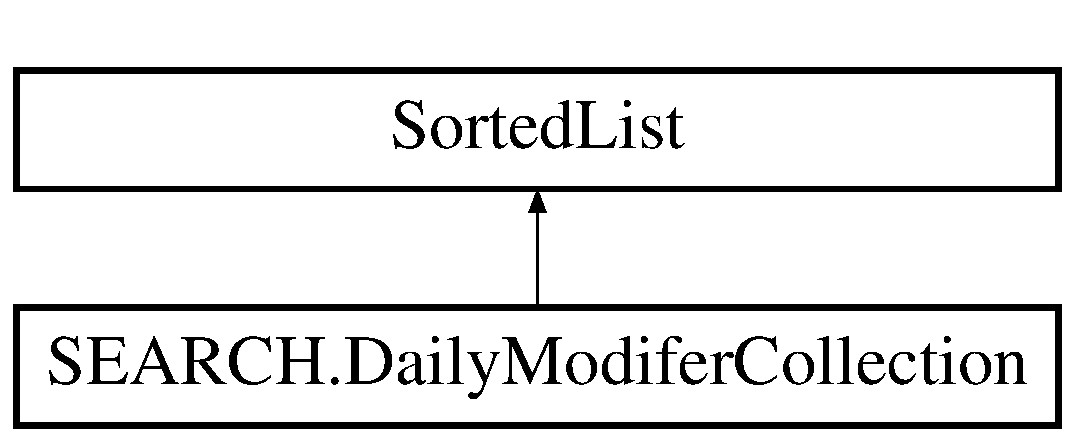
\includegraphics[height=2.000000cm]{class_s_e_a_r_c_h_1_1_daily_modifer_collection}
\end{center}
\end{figure}
\subsection*{Public Member Functions}
\begin{DoxyCompactItemize}
\item 
void \hyperlink{class_s_e_a_r_c_h_1_1_daily_modifer_collection_ad052873914fa09b8bbe3ce3b5086b67c}{advance\-One\-Year} ()
\item 
\hyperlink{class_s_e_a_r_c_h_1_1_daily_modifier}{Daily\-Modifier} \hyperlink{class_s_e_a_r_c_h_1_1_daily_modifer_collection_aff8c3bb772244fc60237f822b93813bc}{get\-First} ()
\item 
\hyperlink{class_s_e_a_r_c_h_1_1_daily_modifier}{Daily\-Modifier} \hyperlink{class_s_e_a_r_c_h_1_1_daily_modifer_collection_ad033612ae50c83785af234f8581ef89c}{get\-Next} ()
\item 
void \hyperlink{class_s_e_a_r_c_h_1_1_daily_modifer_collection_a2bc12bb09a1377704a13af5182c69c92}{reset} ()
\end{DoxyCompactItemize}
\subsection*{Static Public Member Functions}
\begin{DoxyCompactItemize}
\item 
static \hyperlink{class_s_e_a_r_c_h_1_1_daily_modifer_collection}{Daily\-Modifer\-Collection} \hyperlink{class_s_e_a_r_c_h_1_1_daily_modifer_collection_af537ec884ee1035a37b73793ce9c71d2}{Get\-Unique\-Instance} ()
\end{DoxyCompactItemize}
\subsection*{Properties}
\begin{DoxyCompactItemize}
\item 
Date\-Time \hyperlink{class_s_e_a_r_c_h_1_1_daily_modifer_collection_a7679de6a45b07a9050f7c102df533b2a}{Next\-Start\-Date}\hspace{0.3cm}{\ttfamily  \mbox{[}get, set\mbox{]}}
\end{DoxyCompactItemize}


\subsection{Member Function Documentation}
\hypertarget{class_s_e_a_r_c_h_1_1_daily_modifer_collection_ad052873914fa09b8bbe3ce3b5086b67c}{\index{S\-E\-A\-R\-C\-H\-::\-Daily\-Modifer\-Collection@{S\-E\-A\-R\-C\-H\-::\-Daily\-Modifer\-Collection}!advance\-One\-Year@{advance\-One\-Year}}
\index{advance\-One\-Year@{advance\-One\-Year}!SEARCH::DailyModiferCollection@{S\-E\-A\-R\-C\-H\-::\-Daily\-Modifer\-Collection}}
\subsubsection[{advance\-One\-Year}]{\setlength{\rightskip}{0pt plus 5cm}void S\-E\-A\-R\-C\-H.\-Daily\-Modifer\-Collection.\-advance\-One\-Year (
\begin{DoxyParamCaption}
{}
\end{DoxyParamCaption}
)}}\label{class_s_e_a_r_c_h_1_1_daily_modifer_collection_ad052873914fa09b8bbe3ce3b5086b67c}
\hypertarget{class_s_e_a_r_c_h_1_1_daily_modifer_collection_aff8c3bb772244fc60237f822b93813bc}{\index{S\-E\-A\-R\-C\-H\-::\-Daily\-Modifer\-Collection@{S\-E\-A\-R\-C\-H\-::\-Daily\-Modifer\-Collection}!get\-First@{get\-First}}
\index{get\-First@{get\-First}!SEARCH::DailyModiferCollection@{S\-E\-A\-R\-C\-H\-::\-Daily\-Modifer\-Collection}}
\subsubsection[{get\-First}]{\setlength{\rightskip}{0pt plus 5cm}{\bf Daily\-Modifier} S\-E\-A\-R\-C\-H.\-Daily\-Modifer\-Collection.\-get\-First (
\begin{DoxyParamCaption}
{}
\end{DoxyParamCaption}
)}}\label{class_s_e_a_r_c_h_1_1_daily_modifer_collection_aff8c3bb772244fc60237f822b93813bc}
\hypertarget{class_s_e_a_r_c_h_1_1_daily_modifer_collection_ad033612ae50c83785af234f8581ef89c}{\index{S\-E\-A\-R\-C\-H\-::\-Daily\-Modifer\-Collection@{S\-E\-A\-R\-C\-H\-::\-Daily\-Modifer\-Collection}!get\-Next@{get\-Next}}
\index{get\-Next@{get\-Next}!SEARCH::DailyModiferCollection@{S\-E\-A\-R\-C\-H\-::\-Daily\-Modifer\-Collection}}
\subsubsection[{get\-Next}]{\setlength{\rightskip}{0pt plus 5cm}{\bf Daily\-Modifier} S\-E\-A\-R\-C\-H.\-Daily\-Modifer\-Collection.\-get\-Next (
\begin{DoxyParamCaption}
{}
\end{DoxyParamCaption}
)}}\label{class_s_e_a_r_c_h_1_1_daily_modifer_collection_ad033612ae50c83785af234f8581ef89c}
\hypertarget{class_s_e_a_r_c_h_1_1_daily_modifer_collection_af537ec884ee1035a37b73793ce9c71d2}{\index{S\-E\-A\-R\-C\-H\-::\-Daily\-Modifer\-Collection@{S\-E\-A\-R\-C\-H\-::\-Daily\-Modifer\-Collection}!Get\-Unique\-Instance@{Get\-Unique\-Instance}}
\index{Get\-Unique\-Instance@{Get\-Unique\-Instance}!SEARCH::DailyModiferCollection@{S\-E\-A\-R\-C\-H\-::\-Daily\-Modifer\-Collection}}
\subsubsection[{Get\-Unique\-Instance}]{\setlength{\rightskip}{0pt plus 5cm}static {\bf Daily\-Modifer\-Collection} S\-E\-A\-R\-C\-H.\-Daily\-Modifer\-Collection.\-Get\-Unique\-Instance (
\begin{DoxyParamCaption}
{}
\end{DoxyParamCaption}
)\hspace{0.3cm}{\ttfamily [static]}}}\label{class_s_e_a_r_c_h_1_1_daily_modifer_collection_af537ec884ee1035a37b73793ce9c71d2}
\hypertarget{class_s_e_a_r_c_h_1_1_daily_modifer_collection_a2bc12bb09a1377704a13af5182c69c92}{\index{S\-E\-A\-R\-C\-H\-::\-Daily\-Modifer\-Collection@{S\-E\-A\-R\-C\-H\-::\-Daily\-Modifer\-Collection}!reset@{reset}}
\index{reset@{reset}!SEARCH::DailyModiferCollection@{S\-E\-A\-R\-C\-H\-::\-Daily\-Modifer\-Collection}}
\subsubsection[{reset}]{\setlength{\rightskip}{0pt plus 5cm}void S\-E\-A\-R\-C\-H.\-Daily\-Modifer\-Collection.\-reset (
\begin{DoxyParamCaption}
{}
\end{DoxyParamCaption}
)}}\label{class_s_e_a_r_c_h_1_1_daily_modifer_collection_a2bc12bb09a1377704a13af5182c69c92}


\subsection{Property Documentation}
\hypertarget{class_s_e_a_r_c_h_1_1_daily_modifer_collection_a7679de6a45b07a9050f7c102df533b2a}{\index{S\-E\-A\-R\-C\-H\-::\-Daily\-Modifer\-Collection@{S\-E\-A\-R\-C\-H\-::\-Daily\-Modifer\-Collection}!Next\-Start\-Date@{Next\-Start\-Date}}
\index{Next\-Start\-Date@{Next\-Start\-Date}!SEARCH::DailyModiferCollection@{S\-E\-A\-R\-C\-H\-::\-Daily\-Modifer\-Collection}}
\subsubsection[{Next\-Start\-Date}]{\setlength{\rightskip}{0pt plus 5cm}Date\-Time S\-E\-A\-R\-C\-H.\-Daily\-Modifer\-Collection.\-Next\-Start\-Date\hspace{0.3cm}{\ttfamily [get]}, {\ttfamily [set]}}}\label{class_s_e_a_r_c_h_1_1_daily_modifer_collection_a7679de6a45b07a9050f7c102df533b2a}


The documentation for this class was generated from the following file\-:\begin{DoxyCompactItemize}
\item 
Desktop/vlog4net\-A\-R\-C10\-\_\-64\-\_\-newhoming/\-Data\-Centric/\hyperlink{_daily_modifer_collection_8cs}{Daily\-Modifer\-Collection.\-cs}\end{DoxyCompactItemize}

\hypertarget{class_s_e_a_r_c_h_1_1_daily_modifier}{\section{S\-E\-A\-R\-C\-H.\-Daily\-Modifier Class Reference}
\label{class_s_e_a_r_c_h_1_1_daily_modifier}\index{S\-E\-A\-R\-C\-H.\-Daily\-Modifier@{S\-E\-A\-R\-C\-H.\-Daily\-Modifier}}
}


A modifier that hangs out for a certain number of days  


Inheritance diagram for S\-E\-A\-R\-C\-H.\-Daily\-Modifier\-:\begin{figure}[H]
\begin{center}
\leavevmode
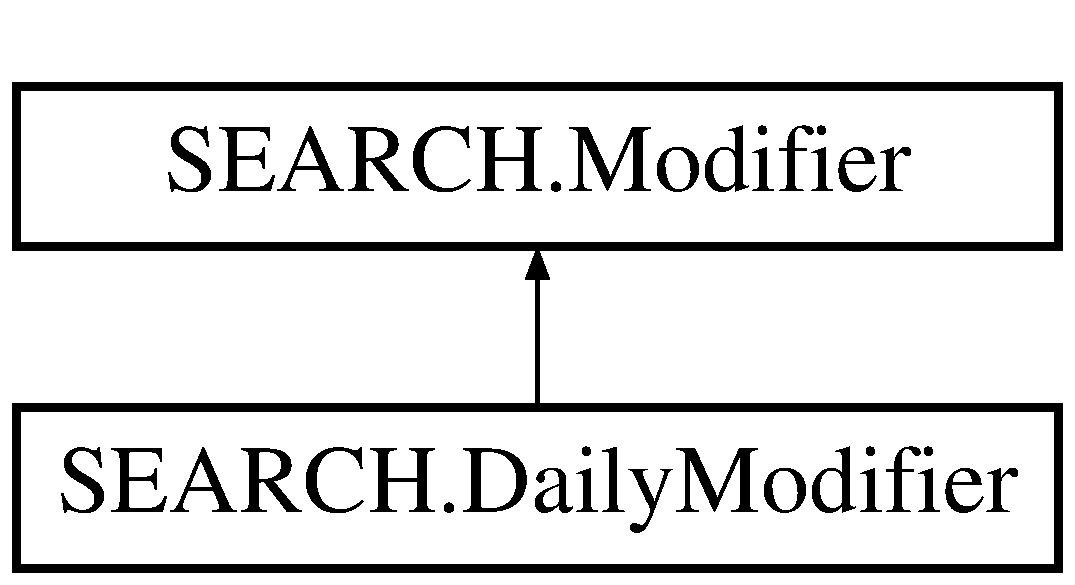
\includegraphics[height=2.000000cm]{class_s_e_a_r_c_h_1_1_daily_modifier}
\end{center}
\end{figure}
\subsection*{Public Member Functions}
\begin{DoxyCompactItemize}
\item 
void \hyperlink{class_s_e_a_r_c_h_1_1_daily_modifier_a92b4972ae3d4cc4f4557d859e1de1942}{advance\-One\-Year} ()
\end{DoxyCompactItemize}
\subsection*{Properties}
\begin{DoxyCompactItemize}
\item 
Date\-Time \hyperlink{class_s_e_a_r_c_h_1_1_daily_modifier_a4b8518a5ae505e906256c155ce090122}{Start\-Date}\hspace{0.3cm}{\ttfamily  \mbox{[}get, set\mbox{]}}
\end{DoxyCompactItemize}


\subsection{Detailed Description}
A modifier that hangs out for a certain number of days 



\subsection{Member Function Documentation}
\hypertarget{class_s_e_a_r_c_h_1_1_daily_modifier_a92b4972ae3d4cc4f4557d859e1de1942}{\index{S\-E\-A\-R\-C\-H\-::\-Daily\-Modifier@{S\-E\-A\-R\-C\-H\-::\-Daily\-Modifier}!advance\-One\-Year@{advance\-One\-Year}}
\index{advance\-One\-Year@{advance\-One\-Year}!SEARCH::DailyModifier@{S\-E\-A\-R\-C\-H\-::\-Daily\-Modifier}}
\subsubsection[{advance\-One\-Year}]{\setlength{\rightskip}{0pt plus 5cm}void S\-E\-A\-R\-C\-H.\-Daily\-Modifier.\-advance\-One\-Year (
\begin{DoxyParamCaption}
{}
\end{DoxyParamCaption}
)}}\label{class_s_e_a_r_c_h_1_1_daily_modifier_a92b4972ae3d4cc4f4557d859e1de1942}


\subsection{Property Documentation}
\hypertarget{class_s_e_a_r_c_h_1_1_daily_modifier_a4b8518a5ae505e906256c155ce090122}{\index{S\-E\-A\-R\-C\-H\-::\-Daily\-Modifier@{S\-E\-A\-R\-C\-H\-::\-Daily\-Modifier}!Start\-Date@{Start\-Date}}
\index{Start\-Date@{Start\-Date}!SEARCH::DailyModifier@{S\-E\-A\-R\-C\-H\-::\-Daily\-Modifier}}
\subsubsection[{Start\-Date}]{\setlength{\rightskip}{0pt plus 5cm}Date\-Time S\-E\-A\-R\-C\-H.\-Daily\-Modifier.\-Start\-Date\hspace{0.3cm}{\ttfamily [get]}, {\ttfamily [set]}}}\label{class_s_e_a_r_c_h_1_1_daily_modifier_a4b8518a5ae505e906256c155ce090122}


The documentation for this class was generated from the following file\-:\begin{DoxyCompactItemize}
\item 
Desktop/vlog4net\-A\-R\-C10\-\_\-64\-\_\-newhoming/\-Data\-Centric/\hyperlink{_daily_modifier_8cs}{Daily\-Modifier.\-cs}\end{DoxyCompactItemize}

\hypertarget{class_s_e_a_r_c_h_1_1_data_manipulator}{\section{S\-E\-A\-R\-C\-H.\-Data\-Manipulator Class Reference}
\label{class_s_e_a_r_c_h_1_1_data_manipulator}\index{S\-E\-A\-R\-C\-H.\-Data\-Manipulator@{S\-E\-A\-R\-C\-H.\-Data\-Manipulator}}
}
\subsection*{Public Member Functions}
\begin{DoxyCompactItemize}
\item 
\hyperlink{class_s_e_a_r_c_h_1_1_data_manipulator_ad272a7582d505115ef08116dee408b06}{Data\-Manipulator} (string file\-Name)
\item 
\hyperlink{class_s_e_a_r_c_h_1_1_data_manipulator_acc2804681760f312bb35d3fc3b1364d7}{Data\-Manipulator} ()
\item 
void \hyperlink{class_s_e_a_r_c_h_1_1_data_manipulator_a42ccdfd6112fd36dcca324bb6981b179}{Add\-Field} (string data\-Type, string field\-Name, object value, string layer\-To\-Add\-Field\-To)
\item 
I\-Feature\-Class \hyperlink{class_s_e_a_r_c_h_1_1_data_manipulator_a1a611050f8b2b27543719ec80084ee3b}{Add\-Home\-Range\-Poly\-Gon} (string out\-File\-Name, I\-Polygon in\-Home\-Range)
\item 
void \hyperlink{class_s_e_a_r_c_h_1_1_data_manipulator_a9b3344a155bb79f1961d9c9ef8a88173}{Clean\-Union\-Results} (string Union\-Path)
\item 
void \hyperlink{class_s_e_a_r_c_h_1_1_data_manipulator_a2dded11d12d221f882b38b0ffae0f822}{Clip} (string in\-File\-Name\-Clip\-From, string in\-File\-Name\-Clip\-Feature, string out\-File\-Name)
\item 
void \hyperlink{class_s_e_a_r_c_h_1_1_data_manipulator_aebe754b172c0541c922ab3b0fbb14d9f}{Copy\-To\-Anotherl\-Map} (string New\-Map\-Path, string Old\-Map\-Path)
\item 
I\-Feature\-Class \hyperlink{class_s_e_a_r_c_h_1_1_data_manipulator_a8f12cda59193695b74bedfb48345f677}{Create\-Empty\-Feature\-Class} (string in\-File\-Name, string feature\-Type)
\item 
bool \hyperlink{class_s_e_a_r_c_h_1_1_data_manipulator_adf7dc52cf6e35b6444455c9e4278f85f}{Create\-Step\-Map} (string in\-File\-Path, List$<$ I\-Point $>$ in\-Steps)
\item 
void \hyperlink{class_s_e_a_r_c_h_1_1_data_manipulator_aa5beef05be975078b12d25244a697cf1}{Delete\-All\-Features} (string in\-File\-Name)
\item 
void \hyperlink{class_s_e_a_r_c_h_1_1_data_manipulator_acccef378f87deaa4d7daf38e9810704a}{Delete\-All\-Features2} (string in\-File\-Name)
\item 
void \hyperlink{class_s_e_a_r_c_h_1_1_data_manipulator_ab68ecc2a1bf4bb1bd9f4e70559e82e4b}{Dissolve} (string in\-File, string out\-File, string Field\-Names)
\item 
I\-Feature\-Class \hyperlink{class_s_e_a_r_c_h_1_1_data_manipulator_a5406f2d07d84b70ced89f902a5441626}{Dissolve\-And\-Return} (string in\-File, string out\-File, string Field\-Names)
\item 
I\-Feature\-Class \hyperlink{class_s_e_a_r_c_h_1_1_data_manipulator_a70fda64cc5a27367132f78c6214fffaf}{Dissolve\-By\-Sex\-And\-Return} (I\-Feature\-Class in\-F\-E, string out\-File, string sex)
\item 
I\-Feature\-Class \hyperlink{class_s_e_a_r_c_h_1_1_data_manipulator_a87df299adbf7ac4afc2c39893e89d80b}{Get\-Feature\-Class} (string in\-File\-Name)
\item 
I\-Feature\-Class \hyperlink{class_s_e_a_r_c_h_1_1_data_manipulator_acc4b6dc1bf9c53126329df3e5897d160}{Get\-Feature\-Class} (string path, string file\-Name)
\item 
I\-Feature\-Class \hyperlink{class_s_e_a_r_c_h_1_1_data_manipulator_a10156760991b383df31c40807bebf045}{Get\-Newly\-Added\-To\-Social\-Map\-Polygons} (string in\-File\-Name, string out\-File\-Name)
\item 
int \hyperlink{class_s_e_a_r_c_h_1_1_data_manipulator_ac328b16927b1f874e8fb7a2ffbf82e6a}{Get\-Row\-Count} (string in\-File\-Name)
\item 
int \hyperlink{class_s_e_a_r_c_h_1_1_data_manipulator_afb9797833d39815381d5e1231fe70c94}{Get\-Row\-Count} (I\-Feature\-Class in\-F\-C)
\item 
I\-Feature\-Class \hyperlink{class_s_e_a_r_c_h_1_1_data_manipulator_af1470bc6c7509bb80efff28d618984f1}{Get\-Suitable\-Polygons} (string in\-File\-Name, string sex)
\item 
I\-Feature\-Class \hyperlink{class_s_e_a_r_c_h_1_1_data_manipulator_a5550febcb2a5945eb7cb0d5a52377c4b}{Get\-Suitable\-Polygons} (string in\-File\-Name, string sex, string out\-File\-Name)
\item 
I\-Feature\-Class \hyperlink{class_s_e_a_r_c_h_1_1_data_manipulator_a55736d637b0508e504de339a2071ef67}{Intersect\-Features} (string in\-Features\-Names, string out\-Feature\-Name)
\item 
I\-Feature\-Class \hyperlink{class_s_e_a_r_c_h_1_1_data_manipulator_a9ec0c428301da7b714399d90a62c4015}{Intersect\-Features} (string in\-Features\-Names, string out\-Feature\-Name, string ignore\-Message)
\item 
void \hyperlink{class_s_e_a_r_c_h_1_1_data_manipulator_a05d9b0670cf10fbe3ea6f8abc15c5518}{Join\-Layers} (string layer\-Name1, string layer\-Name2)
\item 
bool \hyperlink{class_s_e_a_r_c_h_1_1_data_manipulator_ad0e17c3827e778686a07b3389f3578f2}{Make\-Time\-Step} (string in\-File\-Name, string out\-File\-Name, I\-Point from, I\-Point to)
\item 
bool \hyperlink{class_s_e_a_r_c_h_1_1_data_manipulator_a161fb3d98335b7c221e41ec5dea167fb}{Make\-Dissolved\-Time\-Step} (string in\-Full\-File\-Path, string dissovle\-Path, I\-Polygon in\-Poly1, I\-Polygon in\-Poly2)
\item 
void \hyperlink{class_s_e_a_r_c_h_1_1_data_manipulator_a6d8318737bc98a773b11520c09e7c686}{make\-Home\-Range\-Selection\-Map} (string step\-Map\-Name, string animal\-Memory\-Map\-Name)
\item 
I\-Polyline \hyperlink{class_s_e_a_r_c_h_1_1_data_manipulator_a1ac31ad7044d93328664940f878f524b}{Make\-Poly\-Line} (I\-Point from, I\-Point to)
\item 
void \hyperlink{class_s_e_a_r_c_h_1_1_data_manipulator_af9395181eb8f8b31b9c24ff5a5b4bb26}{Multi\-To\-Single\-Part} (string in\-File\-Name, string out\-File\-Name)
\item 
void \hyperlink{class_s_e_a_r_c_h_1_1_data_manipulator_a08e359c8110275e7b4b56baac9af6cff}{Remove\-Extra\-Fields} (string in\-Full\-File\-Path, string List\-Of\-Fields)
\item 
I\-Feature\-Class \hyperlink{class_s_e_a_r_c_h_1_1_data_manipulator_abbb229d1c972fed92c2c560c69c050fb}{Set\-Suitable\-Steps} (string in\-Point\-File\-Name, List$<$ I\-Point $>$ in\-Points, string in\-Memory\-Map)
\item 
bool \hyperlink{class_s_e_a_r_c_h_1_1_data_manipulator_ae9ea4720dd568b2916b65a4a08cdfac5}{Union\-Animal\-Clip\-Data} (string in\-Animal\-Path, string in\-Clip\-Path, string out\-Put\-File\-Name)
\item 
void \hyperlink{class_s_e_a_r_c_h_1_1_data_manipulator_adda1d4220cd5a6ecef7185d0665ec48b}{Union\-Home\-Range} (string in\-Temp\-Home\-Range\-Path, string in\-Social\-Map\-Path, string out\-Put\-File\-Name)
\end{DoxyCompactItemize}


\subsection{Constructor \& Destructor Documentation}
\hypertarget{class_s_e_a_r_c_h_1_1_data_manipulator_ad272a7582d505115ef08116dee408b06}{\index{S\-E\-A\-R\-C\-H\-::\-Data\-Manipulator@{S\-E\-A\-R\-C\-H\-::\-Data\-Manipulator}!Data\-Manipulator@{Data\-Manipulator}}
\index{Data\-Manipulator@{Data\-Manipulator}!SEARCH::DataManipulator@{S\-E\-A\-R\-C\-H\-::\-Data\-Manipulator}}
\subsubsection[{Data\-Manipulator}]{\setlength{\rightskip}{0pt plus 5cm}S\-E\-A\-R\-C\-H.\-Data\-Manipulator.\-Data\-Manipulator (
\begin{DoxyParamCaption}
\item[{string}]{file\-Name}
\end{DoxyParamCaption}
)}}\label{class_s_e_a_r_c_h_1_1_data_manipulator_ad272a7582d505115ef08116dee408b06}
\hypertarget{class_s_e_a_r_c_h_1_1_data_manipulator_acc2804681760f312bb35d3fc3b1364d7}{\index{S\-E\-A\-R\-C\-H\-::\-Data\-Manipulator@{S\-E\-A\-R\-C\-H\-::\-Data\-Manipulator}!Data\-Manipulator@{Data\-Manipulator}}
\index{Data\-Manipulator@{Data\-Manipulator}!SEARCH::DataManipulator@{S\-E\-A\-R\-C\-H\-::\-Data\-Manipulator}}
\subsubsection[{Data\-Manipulator}]{\setlength{\rightskip}{0pt plus 5cm}S\-E\-A\-R\-C\-H.\-Data\-Manipulator.\-Data\-Manipulator (
\begin{DoxyParamCaption}
{}
\end{DoxyParamCaption}
)}}\label{class_s_e_a_r_c_h_1_1_data_manipulator_acc2804681760f312bb35d3fc3b1364d7}


\subsection{Member Function Documentation}
\hypertarget{class_s_e_a_r_c_h_1_1_data_manipulator_a42ccdfd6112fd36dcca324bb6981b179}{\index{S\-E\-A\-R\-C\-H\-::\-Data\-Manipulator@{S\-E\-A\-R\-C\-H\-::\-Data\-Manipulator}!Add\-Field@{Add\-Field}}
\index{Add\-Field@{Add\-Field}!SEARCH::DataManipulator@{S\-E\-A\-R\-C\-H\-::\-Data\-Manipulator}}
\subsubsection[{Add\-Field}]{\setlength{\rightskip}{0pt plus 5cm}void S\-E\-A\-R\-C\-H.\-Data\-Manipulator.\-Add\-Field (
\begin{DoxyParamCaption}
\item[{string}]{data\-Type, }
\item[{string}]{field\-Name, }
\item[{object}]{value, }
\item[{string}]{layer\-To\-Add\-Field\-To}
\end{DoxyParamCaption}
)}}\label{class_s_e_a_r_c_h_1_1_data_manipulator_a42ccdfd6112fd36dcca324bb6981b179}
\hypertarget{class_s_e_a_r_c_h_1_1_data_manipulator_a1a611050f8b2b27543719ec80084ee3b}{\index{S\-E\-A\-R\-C\-H\-::\-Data\-Manipulator@{S\-E\-A\-R\-C\-H\-::\-Data\-Manipulator}!Add\-Home\-Range\-Poly\-Gon@{Add\-Home\-Range\-Poly\-Gon}}
\index{Add\-Home\-Range\-Poly\-Gon@{Add\-Home\-Range\-Poly\-Gon}!SEARCH::DataManipulator@{S\-E\-A\-R\-C\-H\-::\-Data\-Manipulator}}
\subsubsection[{Add\-Home\-Range\-Poly\-Gon}]{\setlength{\rightskip}{0pt plus 5cm}I\-Feature\-Class S\-E\-A\-R\-C\-H.\-Data\-Manipulator.\-Add\-Home\-Range\-Poly\-Gon (
\begin{DoxyParamCaption}
\item[{string}]{out\-File\-Name, }
\item[{I\-Polygon}]{in\-Home\-Range}
\end{DoxyParamCaption}
)}}\label{class_s_e_a_r_c_h_1_1_data_manipulator_a1a611050f8b2b27543719ec80084ee3b}
\hypertarget{class_s_e_a_r_c_h_1_1_data_manipulator_a9b3344a155bb79f1961d9c9ef8a88173}{\index{S\-E\-A\-R\-C\-H\-::\-Data\-Manipulator@{S\-E\-A\-R\-C\-H\-::\-Data\-Manipulator}!Clean\-Union\-Results@{Clean\-Union\-Results}}
\index{Clean\-Union\-Results@{Clean\-Union\-Results}!SEARCH::DataManipulator@{S\-E\-A\-R\-C\-H\-::\-Data\-Manipulator}}
\subsubsection[{Clean\-Union\-Results}]{\setlength{\rightskip}{0pt plus 5cm}void S\-E\-A\-R\-C\-H.\-Data\-Manipulator.\-Clean\-Union\-Results (
\begin{DoxyParamCaption}
\item[{string}]{Union\-Path}
\end{DoxyParamCaption}
)}}\label{class_s_e_a_r_c_h_1_1_data_manipulator_a9b3344a155bb79f1961d9c9ef8a88173}
\hypertarget{class_s_e_a_r_c_h_1_1_data_manipulator_a2dded11d12d221f882b38b0ffae0f822}{\index{S\-E\-A\-R\-C\-H\-::\-Data\-Manipulator@{S\-E\-A\-R\-C\-H\-::\-Data\-Manipulator}!Clip@{Clip}}
\index{Clip@{Clip}!SEARCH::DataManipulator@{S\-E\-A\-R\-C\-H\-::\-Data\-Manipulator}}
\subsubsection[{Clip}]{\setlength{\rightskip}{0pt plus 5cm}void S\-E\-A\-R\-C\-H.\-Data\-Manipulator.\-Clip (
\begin{DoxyParamCaption}
\item[{string}]{in\-File\-Name\-Clip\-From, }
\item[{string}]{in\-File\-Name\-Clip\-Feature, }
\item[{string}]{out\-File\-Name}
\end{DoxyParamCaption}
)}}\label{class_s_e_a_r_c_h_1_1_data_manipulator_a2dded11d12d221f882b38b0ffae0f822}
\hypertarget{class_s_e_a_r_c_h_1_1_data_manipulator_aebe754b172c0541c922ab3b0fbb14d9f}{\index{S\-E\-A\-R\-C\-H\-::\-Data\-Manipulator@{S\-E\-A\-R\-C\-H\-::\-Data\-Manipulator}!Copy\-To\-Anotherl\-Map@{Copy\-To\-Anotherl\-Map}}
\index{Copy\-To\-Anotherl\-Map@{Copy\-To\-Anotherl\-Map}!SEARCH::DataManipulator@{S\-E\-A\-R\-C\-H\-::\-Data\-Manipulator}}
\subsubsection[{Copy\-To\-Anotherl\-Map}]{\setlength{\rightskip}{0pt plus 5cm}void S\-E\-A\-R\-C\-H.\-Data\-Manipulator.\-Copy\-To\-Anotherl\-Map (
\begin{DoxyParamCaption}
\item[{string}]{New\-Map\-Path, }
\item[{string}]{Old\-Map\-Path}
\end{DoxyParamCaption}
)}}\label{class_s_e_a_r_c_h_1_1_data_manipulator_aebe754b172c0541c922ab3b0fbb14d9f}
\hypertarget{class_s_e_a_r_c_h_1_1_data_manipulator_a8f12cda59193695b74bedfb48345f677}{\index{S\-E\-A\-R\-C\-H\-::\-Data\-Manipulator@{S\-E\-A\-R\-C\-H\-::\-Data\-Manipulator}!Create\-Empty\-Feature\-Class@{Create\-Empty\-Feature\-Class}}
\index{Create\-Empty\-Feature\-Class@{Create\-Empty\-Feature\-Class}!SEARCH::DataManipulator@{S\-E\-A\-R\-C\-H\-::\-Data\-Manipulator}}
\subsubsection[{Create\-Empty\-Feature\-Class}]{\setlength{\rightskip}{0pt plus 5cm}I\-Feature\-Class S\-E\-A\-R\-C\-H.\-Data\-Manipulator.\-Create\-Empty\-Feature\-Class (
\begin{DoxyParamCaption}
\item[{string}]{in\-File\-Name, }
\item[{string}]{feature\-Type}
\end{DoxyParamCaption}
)}}\label{class_s_e_a_r_c_h_1_1_data_manipulator_a8f12cda59193695b74bedfb48345f677}
\hypertarget{class_s_e_a_r_c_h_1_1_data_manipulator_adf7dc52cf6e35b6444455c9e4278f85f}{\index{S\-E\-A\-R\-C\-H\-::\-Data\-Manipulator@{S\-E\-A\-R\-C\-H\-::\-Data\-Manipulator}!Create\-Step\-Map@{Create\-Step\-Map}}
\index{Create\-Step\-Map@{Create\-Step\-Map}!SEARCH::DataManipulator@{S\-E\-A\-R\-C\-H\-::\-Data\-Manipulator}}
\subsubsection[{Create\-Step\-Map}]{\setlength{\rightskip}{0pt plus 5cm}bool S\-E\-A\-R\-C\-H.\-Data\-Manipulator.\-Create\-Step\-Map (
\begin{DoxyParamCaption}
\item[{string}]{in\-File\-Path, }
\item[{List$<$ I\-Point $>$}]{in\-Steps}
\end{DoxyParamCaption}
)}}\label{class_s_e_a_r_c_h_1_1_data_manipulator_adf7dc52cf6e35b6444455c9e4278f85f}
\hypertarget{class_s_e_a_r_c_h_1_1_data_manipulator_aa5beef05be975078b12d25244a697cf1}{\index{S\-E\-A\-R\-C\-H\-::\-Data\-Manipulator@{S\-E\-A\-R\-C\-H\-::\-Data\-Manipulator}!Delete\-All\-Features@{Delete\-All\-Features}}
\index{Delete\-All\-Features@{Delete\-All\-Features}!SEARCH::DataManipulator@{S\-E\-A\-R\-C\-H\-::\-Data\-Manipulator}}
\subsubsection[{Delete\-All\-Features}]{\setlength{\rightskip}{0pt plus 5cm}void S\-E\-A\-R\-C\-H.\-Data\-Manipulator.\-Delete\-All\-Features (
\begin{DoxyParamCaption}
\item[{string}]{in\-File\-Name}
\end{DoxyParamCaption}
)}}\label{class_s_e_a_r_c_h_1_1_data_manipulator_aa5beef05be975078b12d25244a697cf1}
\hypertarget{class_s_e_a_r_c_h_1_1_data_manipulator_acccef378f87deaa4d7daf38e9810704a}{\index{S\-E\-A\-R\-C\-H\-::\-Data\-Manipulator@{S\-E\-A\-R\-C\-H\-::\-Data\-Manipulator}!Delete\-All\-Features2@{Delete\-All\-Features2}}
\index{Delete\-All\-Features2@{Delete\-All\-Features2}!SEARCH::DataManipulator@{S\-E\-A\-R\-C\-H\-::\-Data\-Manipulator}}
\subsubsection[{Delete\-All\-Features2}]{\setlength{\rightskip}{0pt plus 5cm}void S\-E\-A\-R\-C\-H.\-Data\-Manipulator.\-Delete\-All\-Features2 (
\begin{DoxyParamCaption}
\item[{string}]{in\-File\-Name}
\end{DoxyParamCaption}
)}}\label{class_s_e_a_r_c_h_1_1_data_manipulator_acccef378f87deaa4d7daf38e9810704a}
\hypertarget{class_s_e_a_r_c_h_1_1_data_manipulator_ab68ecc2a1bf4bb1bd9f4e70559e82e4b}{\index{S\-E\-A\-R\-C\-H\-::\-Data\-Manipulator@{S\-E\-A\-R\-C\-H\-::\-Data\-Manipulator}!Dissolve@{Dissolve}}
\index{Dissolve@{Dissolve}!SEARCH::DataManipulator@{S\-E\-A\-R\-C\-H\-::\-Data\-Manipulator}}
\subsubsection[{Dissolve}]{\setlength{\rightskip}{0pt plus 5cm}void S\-E\-A\-R\-C\-H.\-Data\-Manipulator.\-Dissolve (
\begin{DoxyParamCaption}
\item[{string}]{in\-File, }
\item[{string}]{out\-File, }
\item[{string}]{Field\-Names}
\end{DoxyParamCaption}
)}}\label{class_s_e_a_r_c_h_1_1_data_manipulator_ab68ecc2a1bf4bb1bd9f4e70559e82e4b}
\hypertarget{class_s_e_a_r_c_h_1_1_data_manipulator_a5406f2d07d84b70ced89f902a5441626}{\index{S\-E\-A\-R\-C\-H\-::\-Data\-Manipulator@{S\-E\-A\-R\-C\-H\-::\-Data\-Manipulator}!Dissolve\-And\-Return@{Dissolve\-And\-Return}}
\index{Dissolve\-And\-Return@{Dissolve\-And\-Return}!SEARCH::DataManipulator@{S\-E\-A\-R\-C\-H\-::\-Data\-Manipulator}}
\subsubsection[{Dissolve\-And\-Return}]{\setlength{\rightskip}{0pt plus 5cm}I\-Feature\-Class S\-E\-A\-R\-C\-H.\-Data\-Manipulator.\-Dissolve\-And\-Return (
\begin{DoxyParamCaption}
\item[{string}]{in\-File, }
\item[{string}]{out\-File, }
\item[{string}]{Field\-Names}
\end{DoxyParamCaption}
)}}\label{class_s_e_a_r_c_h_1_1_data_manipulator_a5406f2d07d84b70ced89f902a5441626}
\hypertarget{class_s_e_a_r_c_h_1_1_data_manipulator_a70fda64cc5a27367132f78c6214fffaf}{\index{S\-E\-A\-R\-C\-H\-::\-Data\-Manipulator@{S\-E\-A\-R\-C\-H\-::\-Data\-Manipulator}!Dissolve\-By\-Sex\-And\-Return@{Dissolve\-By\-Sex\-And\-Return}}
\index{Dissolve\-By\-Sex\-And\-Return@{Dissolve\-By\-Sex\-And\-Return}!SEARCH::DataManipulator@{S\-E\-A\-R\-C\-H\-::\-Data\-Manipulator}}
\subsubsection[{Dissolve\-By\-Sex\-And\-Return}]{\setlength{\rightskip}{0pt plus 5cm}I\-Feature\-Class S\-E\-A\-R\-C\-H.\-Data\-Manipulator.\-Dissolve\-By\-Sex\-And\-Return (
\begin{DoxyParamCaption}
\item[{I\-Feature\-Class}]{in\-F\-E, }
\item[{string}]{out\-File, }
\item[{string}]{sex}
\end{DoxyParamCaption}
)}}\label{class_s_e_a_r_c_h_1_1_data_manipulator_a70fda64cc5a27367132f78c6214fffaf}
\hypertarget{class_s_e_a_r_c_h_1_1_data_manipulator_a87df299adbf7ac4afc2c39893e89d80b}{\index{S\-E\-A\-R\-C\-H\-::\-Data\-Manipulator@{S\-E\-A\-R\-C\-H\-::\-Data\-Manipulator}!Get\-Feature\-Class@{Get\-Feature\-Class}}
\index{Get\-Feature\-Class@{Get\-Feature\-Class}!SEARCH::DataManipulator@{S\-E\-A\-R\-C\-H\-::\-Data\-Manipulator}}
\subsubsection[{Get\-Feature\-Class}]{\setlength{\rightskip}{0pt plus 5cm}I\-Feature\-Class S\-E\-A\-R\-C\-H.\-Data\-Manipulator.\-Get\-Feature\-Class (
\begin{DoxyParamCaption}
\item[{string}]{in\-File\-Name}
\end{DoxyParamCaption}
)}}\label{class_s_e_a_r_c_h_1_1_data_manipulator_a87df299adbf7ac4afc2c39893e89d80b}
\hypertarget{class_s_e_a_r_c_h_1_1_data_manipulator_acc4b6dc1bf9c53126329df3e5897d160}{\index{S\-E\-A\-R\-C\-H\-::\-Data\-Manipulator@{S\-E\-A\-R\-C\-H\-::\-Data\-Manipulator}!Get\-Feature\-Class@{Get\-Feature\-Class}}
\index{Get\-Feature\-Class@{Get\-Feature\-Class}!SEARCH::DataManipulator@{S\-E\-A\-R\-C\-H\-::\-Data\-Manipulator}}
\subsubsection[{Get\-Feature\-Class}]{\setlength{\rightskip}{0pt plus 5cm}I\-Feature\-Class S\-E\-A\-R\-C\-H.\-Data\-Manipulator.\-Get\-Feature\-Class (
\begin{DoxyParamCaption}
\item[{string}]{path, }
\item[{string}]{file\-Name}
\end{DoxyParamCaption}
)}}\label{class_s_e_a_r_c_h_1_1_data_manipulator_acc4b6dc1bf9c53126329df3e5897d160}
\hypertarget{class_s_e_a_r_c_h_1_1_data_manipulator_a10156760991b383df31c40807bebf045}{\index{S\-E\-A\-R\-C\-H\-::\-Data\-Manipulator@{S\-E\-A\-R\-C\-H\-::\-Data\-Manipulator}!Get\-Newly\-Added\-To\-Social\-Map\-Polygons@{Get\-Newly\-Added\-To\-Social\-Map\-Polygons}}
\index{Get\-Newly\-Added\-To\-Social\-Map\-Polygons@{Get\-Newly\-Added\-To\-Social\-Map\-Polygons}!SEARCH::DataManipulator@{S\-E\-A\-R\-C\-H\-::\-Data\-Manipulator}}
\subsubsection[{Get\-Newly\-Added\-To\-Social\-Map\-Polygons}]{\setlength{\rightskip}{0pt plus 5cm}I\-Feature\-Class S\-E\-A\-R\-C\-H.\-Data\-Manipulator.\-Get\-Newly\-Added\-To\-Social\-Map\-Polygons (
\begin{DoxyParamCaption}
\item[{string}]{in\-File\-Name, }
\item[{string}]{out\-File\-Name}
\end{DoxyParamCaption}
)}}\label{class_s_e_a_r_c_h_1_1_data_manipulator_a10156760991b383df31c40807bebf045}
\hypertarget{class_s_e_a_r_c_h_1_1_data_manipulator_ac328b16927b1f874e8fb7a2ffbf82e6a}{\index{S\-E\-A\-R\-C\-H\-::\-Data\-Manipulator@{S\-E\-A\-R\-C\-H\-::\-Data\-Manipulator}!Get\-Row\-Count@{Get\-Row\-Count}}
\index{Get\-Row\-Count@{Get\-Row\-Count}!SEARCH::DataManipulator@{S\-E\-A\-R\-C\-H\-::\-Data\-Manipulator}}
\subsubsection[{Get\-Row\-Count}]{\setlength{\rightskip}{0pt plus 5cm}int S\-E\-A\-R\-C\-H.\-Data\-Manipulator.\-Get\-Row\-Count (
\begin{DoxyParamCaption}
\item[{string}]{in\-File\-Name}
\end{DoxyParamCaption}
)}}\label{class_s_e_a_r_c_h_1_1_data_manipulator_ac328b16927b1f874e8fb7a2ffbf82e6a}
\hypertarget{class_s_e_a_r_c_h_1_1_data_manipulator_afb9797833d39815381d5e1231fe70c94}{\index{S\-E\-A\-R\-C\-H\-::\-Data\-Manipulator@{S\-E\-A\-R\-C\-H\-::\-Data\-Manipulator}!Get\-Row\-Count@{Get\-Row\-Count}}
\index{Get\-Row\-Count@{Get\-Row\-Count}!SEARCH::DataManipulator@{S\-E\-A\-R\-C\-H\-::\-Data\-Manipulator}}
\subsubsection[{Get\-Row\-Count}]{\setlength{\rightskip}{0pt plus 5cm}int S\-E\-A\-R\-C\-H.\-Data\-Manipulator.\-Get\-Row\-Count (
\begin{DoxyParamCaption}
\item[{I\-Feature\-Class}]{in\-F\-C}
\end{DoxyParamCaption}
)}}\label{class_s_e_a_r_c_h_1_1_data_manipulator_afb9797833d39815381d5e1231fe70c94}
\hypertarget{class_s_e_a_r_c_h_1_1_data_manipulator_af1470bc6c7509bb80efff28d618984f1}{\index{S\-E\-A\-R\-C\-H\-::\-Data\-Manipulator@{S\-E\-A\-R\-C\-H\-::\-Data\-Manipulator}!Get\-Suitable\-Polygons@{Get\-Suitable\-Polygons}}
\index{Get\-Suitable\-Polygons@{Get\-Suitable\-Polygons}!SEARCH::DataManipulator@{S\-E\-A\-R\-C\-H\-::\-Data\-Manipulator}}
\subsubsection[{Get\-Suitable\-Polygons}]{\setlength{\rightskip}{0pt plus 5cm}I\-Feature\-Class S\-E\-A\-R\-C\-H.\-Data\-Manipulator.\-Get\-Suitable\-Polygons (
\begin{DoxyParamCaption}
\item[{string}]{in\-File\-Name, }
\item[{string}]{sex}
\end{DoxyParamCaption}
)}}\label{class_s_e_a_r_c_h_1_1_data_manipulator_af1470bc6c7509bb80efff28d618984f1}
\hypertarget{class_s_e_a_r_c_h_1_1_data_manipulator_a5550febcb2a5945eb7cb0d5a52377c4b}{\index{S\-E\-A\-R\-C\-H\-::\-Data\-Manipulator@{S\-E\-A\-R\-C\-H\-::\-Data\-Manipulator}!Get\-Suitable\-Polygons@{Get\-Suitable\-Polygons}}
\index{Get\-Suitable\-Polygons@{Get\-Suitable\-Polygons}!SEARCH::DataManipulator@{S\-E\-A\-R\-C\-H\-::\-Data\-Manipulator}}
\subsubsection[{Get\-Suitable\-Polygons}]{\setlength{\rightskip}{0pt plus 5cm}I\-Feature\-Class S\-E\-A\-R\-C\-H.\-Data\-Manipulator.\-Get\-Suitable\-Polygons (
\begin{DoxyParamCaption}
\item[{string}]{in\-File\-Name, }
\item[{string}]{sex, }
\item[{string}]{out\-File\-Name}
\end{DoxyParamCaption}
)}}\label{class_s_e_a_r_c_h_1_1_data_manipulator_a5550febcb2a5945eb7cb0d5a52377c4b}
\hypertarget{class_s_e_a_r_c_h_1_1_data_manipulator_a55736d637b0508e504de339a2071ef67}{\index{S\-E\-A\-R\-C\-H\-::\-Data\-Manipulator@{S\-E\-A\-R\-C\-H\-::\-Data\-Manipulator}!Intersect\-Features@{Intersect\-Features}}
\index{Intersect\-Features@{Intersect\-Features}!SEARCH::DataManipulator@{S\-E\-A\-R\-C\-H\-::\-Data\-Manipulator}}
\subsubsection[{Intersect\-Features}]{\setlength{\rightskip}{0pt plus 5cm}I\-Feature\-Class S\-E\-A\-R\-C\-H.\-Data\-Manipulator.\-Intersect\-Features (
\begin{DoxyParamCaption}
\item[{string}]{in\-Features\-Names, }
\item[{string}]{out\-Feature\-Name}
\end{DoxyParamCaption}
)}}\label{class_s_e_a_r_c_h_1_1_data_manipulator_a55736d637b0508e504de339a2071ef67}
\hypertarget{class_s_e_a_r_c_h_1_1_data_manipulator_a9ec0c428301da7b714399d90a62c4015}{\index{S\-E\-A\-R\-C\-H\-::\-Data\-Manipulator@{S\-E\-A\-R\-C\-H\-::\-Data\-Manipulator}!Intersect\-Features@{Intersect\-Features}}
\index{Intersect\-Features@{Intersect\-Features}!SEARCH::DataManipulator@{S\-E\-A\-R\-C\-H\-::\-Data\-Manipulator}}
\subsubsection[{Intersect\-Features}]{\setlength{\rightskip}{0pt plus 5cm}I\-Feature\-Class S\-E\-A\-R\-C\-H.\-Data\-Manipulator.\-Intersect\-Features (
\begin{DoxyParamCaption}
\item[{string}]{in\-Features\-Names, }
\item[{string}]{out\-Feature\-Name, }
\item[{string}]{ignore\-Message}
\end{DoxyParamCaption}
)}}\label{class_s_e_a_r_c_h_1_1_data_manipulator_a9ec0c428301da7b714399d90a62c4015}
\hypertarget{class_s_e_a_r_c_h_1_1_data_manipulator_a05d9b0670cf10fbe3ea6f8abc15c5518}{\index{S\-E\-A\-R\-C\-H\-::\-Data\-Manipulator@{S\-E\-A\-R\-C\-H\-::\-Data\-Manipulator}!Join\-Layers@{Join\-Layers}}
\index{Join\-Layers@{Join\-Layers}!SEARCH::DataManipulator@{S\-E\-A\-R\-C\-H\-::\-Data\-Manipulator}}
\subsubsection[{Join\-Layers}]{\setlength{\rightskip}{0pt plus 5cm}void S\-E\-A\-R\-C\-H.\-Data\-Manipulator.\-Join\-Layers (
\begin{DoxyParamCaption}
\item[{string}]{layer\-Name1, }
\item[{string}]{layer\-Name2}
\end{DoxyParamCaption}
)}}\label{class_s_e_a_r_c_h_1_1_data_manipulator_a05d9b0670cf10fbe3ea6f8abc15c5518}
\hypertarget{class_s_e_a_r_c_h_1_1_data_manipulator_a161fb3d98335b7c221e41ec5dea167fb}{\index{S\-E\-A\-R\-C\-H\-::\-Data\-Manipulator@{S\-E\-A\-R\-C\-H\-::\-Data\-Manipulator}!Make\-Dissolved\-Time\-Step@{Make\-Dissolved\-Time\-Step}}
\index{Make\-Dissolved\-Time\-Step@{Make\-Dissolved\-Time\-Step}!SEARCH::DataManipulator@{S\-E\-A\-R\-C\-H\-::\-Data\-Manipulator}}
\subsubsection[{Make\-Dissolved\-Time\-Step}]{\setlength{\rightskip}{0pt plus 5cm}bool S\-E\-A\-R\-C\-H.\-Data\-Manipulator.\-Make\-Dissolved\-Time\-Step (
\begin{DoxyParamCaption}
\item[{string}]{in\-Full\-File\-Path, }
\item[{string}]{dissovle\-Path, }
\item[{I\-Polygon}]{in\-Poly1, }
\item[{I\-Polygon}]{in\-Poly2}
\end{DoxyParamCaption}
)}}\label{class_s_e_a_r_c_h_1_1_data_manipulator_a161fb3d98335b7c221e41ec5dea167fb}
\hypertarget{class_s_e_a_r_c_h_1_1_data_manipulator_a6d8318737bc98a773b11520c09e7c686}{\index{S\-E\-A\-R\-C\-H\-::\-Data\-Manipulator@{S\-E\-A\-R\-C\-H\-::\-Data\-Manipulator}!make\-Home\-Range\-Selection\-Map@{make\-Home\-Range\-Selection\-Map}}
\index{make\-Home\-Range\-Selection\-Map@{make\-Home\-Range\-Selection\-Map}!SEARCH::DataManipulator@{S\-E\-A\-R\-C\-H\-::\-Data\-Manipulator}}
\subsubsection[{make\-Home\-Range\-Selection\-Map}]{\setlength{\rightskip}{0pt plus 5cm}void S\-E\-A\-R\-C\-H.\-Data\-Manipulator.\-make\-Home\-Range\-Selection\-Map (
\begin{DoxyParamCaption}
\item[{string}]{step\-Map\-Name, }
\item[{string}]{animal\-Memory\-Map\-Name}
\end{DoxyParamCaption}
)}}\label{class_s_e_a_r_c_h_1_1_data_manipulator_a6d8318737bc98a773b11520c09e7c686}
\hypertarget{class_s_e_a_r_c_h_1_1_data_manipulator_a1ac31ad7044d93328664940f878f524b}{\index{S\-E\-A\-R\-C\-H\-::\-Data\-Manipulator@{S\-E\-A\-R\-C\-H\-::\-Data\-Manipulator}!Make\-Poly\-Line@{Make\-Poly\-Line}}
\index{Make\-Poly\-Line@{Make\-Poly\-Line}!SEARCH::DataManipulator@{S\-E\-A\-R\-C\-H\-::\-Data\-Manipulator}}
\subsubsection[{Make\-Poly\-Line}]{\setlength{\rightskip}{0pt plus 5cm}I\-Polyline S\-E\-A\-R\-C\-H.\-Data\-Manipulator.\-Make\-Poly\-Line (
\begin{DoxyParamCaption}
\item[{I\-Point}]{from, }
\item[{I\-Point}]{to}
\end{DoxyParamCaption}
)}}\label{class_s_e_a_r_c_h_1_1_data_manipulator_a1ac31ad7044d93328664940f878f524b}
\hypertarget{class_s_e_a_r_c_h_1_1_data_manipulator_ad0e17c3827e778686a07b3389f3578f2}{\index{S\-E\-A\-R\-C\-H\-::\-Data\-Manipulator@{S\-E\-A\-R\-C\-H\-::\-Data\-Manipulator}!Make\-Time\-Step@{Make\-Time\-Step}}
\index{Make\-Time\-Step@{Make\-Time\-Step}!SEARCH::DataManipulator@{S\-E\-A\-R\-C\-H\-::\-Data\-Manipulator}}
\subsubsection[{Make\-Time\-Step}]{\setlength{\rightskip}{0pt plus 5cm}bool S\-E\-A\-R\-C\-H.\-Data\-Manipulator.\-Make\-Time\-Step (
\begin{DoxyParamCaption}
\item[{string}]{in\-File\-Name, }
\item[{string}]{out\-File\-Name, }
\item[{I\-Point}]{from, }
\item[{I\-Point}]{to}
\end{DoxyParamCaption}
)}}\label{class_s_e_a_r_c_h_1_1_data_manipulator_ad0e17c3827e778686a07b3389f3578f2}
\hypertarget{class_s_e_a_r_c_h_1_1_data_manipulator_af9395181eb8f8b31b9c24ff5a5b4bb26}{\index{S\-E\-A\-R\-C\-H\-::\-Data\-Manipulator@{S\-E\-A\-R\-C\-H\-::\-Data\-Manipulator}!Multi\-To\-Single\-Part@{Multi\-To\-Single\-Part}}
\index{Multi\-To\-Single\-Part@{Multi\-To\-Single\-Part}!SEARCH::DataManipulator@{S\-E\-A\-R\-C\-H\-::\-Data\-Manipulator}}
\subsubsection[{Multi\-To\-Single\-Part}]{\setlength{\rightskip}{0pt plus 5cm}void S\-E\-A\-R\-C\-H.\-Data\-Manipulator.\-Multi\-To\-Single\-Part (
\begin{DoxyParamCaption}
\item[{string}]{in\-File\-Name, }
\item[{string}]{out\-File\-Name}
\end{DoxyParamCaption}
)}}\label{class_s_e_a_r_c_h_1_1_data_manipulator_af9395181eb8f8b31b9c24ff5a5b4bb26}
\hypertarget{class_s_e_a_r_c_h_1_1_data_manipulator_a08e359c8110275e7b4b56baac9af6cff}{\index{S\-E\-A\-R\-C\-H\-::\-Data\-Manipulator@{S\-E\-A\-R\-C\-H\-::\-Data\-Manipulator}!Remove\-Extra\-Fields@{Remove\-Extra\-Fields}}
\index{Remove\-Extra\-Fields@{Remove\-Extra\-Fields}!SEARCH::DataManipulator@{S\-E\-A\-R\-C\-H\-::\-Data\-Manipulator}}
\subsubsection[{Remove\-Extra\-Fields}]{\setlength{\rightskip}{0pt plus 5cm}void S\-E\-A\-R\-C\-H.\-Data\-Manipulator.\-Remove\-Extra\-Fields (
\begin{DoxyParamCaption}
\item[{string}]{in\-Full\-File\-Path, }
\item[{string}]{List\-Of\-Fields}
\end{DoxyParamCaption}
)}}\label{class_s_e_a_r_c_h_1_1_data_manipulator_a08e359c8110275e7b4b56baac9af6cff}
\hypertarget{class_s_e_a_r_c_h_1_1_data_manipulator_abbb229d1c972fed92c2c560c69c050fb}{\index{S\-E\-A\-R\-C\-H\-::\-Data\-Manipulator@{S\-E\-A\-R\-C\-H\-::\-Data\-Manipulator}!Set\-Suitable\-Steps@{Set\-Suitable\-Steps}}
\index{Set\-Suitable\-Steps@{Set\-Suitable\-Steps}!SEARCH::DataManipulator@{S\-E\-A\-R\-C\-H\-::\-Data\-Manipulator}}
\subsubsection[{Set\-Suitable\-Steps}]{\setlength{\rightskip}{0pt plus 5cm}I\-Feature\-Class S\-E\-A\-R\-C\-H.\-Data\-Manipulator.\-Set\-Suitable\-Steps (
\begin{DoxyParamCaption}
\item[{string}]{in\-Point\-File\-Name, }
\item[{List$<$ I\-Point $>$}]{in\-Points, }
\item[{string}]{in\-Memory\-Map}
\end{DoxyParamCaption}
)}}\label{class_s_e_a_r_c_h_1_1_data_manipulator_abbb229d1c972fed92c2c560c69c050fb}
\hypertarget{class_s_e_a_r_c_h_1_1_data_manipulator_ae9ea4720dd568b2916b65a4a08cdfac5}{\index{S\-E\-A\-R\-C\-H\-::\-Data\-Manipulator@{S\-E\-A\-R\-C\-H\-::\-Data\-Manipulator}!Union\-Animal\-Clip\-Data@{Union\-Animal\-Clip\-Data}}
\index{Union\-Animal\-Clip\-Data@{Union\-Animal\-Clip\-Data}!SEARCH::DataManipulator@{S\-E\-A\-R\-C\-H\-::\-Data\-Manipulator}}
\subsubsection[{Union\-Animal\-Clip\-Data}]{\setlength{\rightskip}{0pt plus 5cm}bool S\-E\-A\-R\-C\-H.\-Data\-Manipulator.\-Union\-Animal\-Clip\-Data (
\begin{DoxyParamCaption}
\item[{string}]{in\-Animal\-Path, }
\item[{string}]{in\-Clip\-Path, }
\item[{string}]{out\-Put\-File\-Name}
\end{DoxyParamCaption}
)}}\label{class_s_e_a_r_c_h_1_1_data_manipulator_ae9ea4720dd568b2916b65a4a08cdfac5}
\hypertarget{class_s_e_a_r_c_h_1_1_data_manipulator_adda1d4220cd5a6ecef7185d0665ec48b}{\index{S\-E\-A\-R\-C\-H\-::\-Data\-Manipulator@{S\-E\-A\-R\-C\-H\-::\-Data\-Manipulator}!Union\-Home\-Range@{Union\-Home\-Range}}
\index{Union\-Home\-Range@{Union\-Home\-Range}!SEARCH::DataManipulator@{S\-E\-A\-R\-C\-H\-::\-Data\-Manipulator}}
\subsubsection[{Union\-Home\-Range}]{\setlength{\rightskip}{0pt plus 5cm}void S\-E\-A\-R\-C\-H.\-Data\-Manipulator.\-Union\-Home\-Range (
\begin{DoxyParamCaption}
\item[{string}]{in\-Temp\-Home\-Range\-Path, }
\item[{string}]{in\-Social\-Map\-Path, }
\item[{string}]{out\-Put\-File\-Name}
\end{DoxyParamCaption}
)}}\label{class_s_e_a_r_c_h_1_1_data_manipulator_adda1d4220cd5a6ecef7185d0665ec48b}


The documentation for this class was generated from the following file\-:\begin{DoxyCompactItemize}
\item 
Desktop/vlog4net\-A\-R\-C10\-\_\-64\-\_\-newhoming/\-Data\-Centric/\hyperlink{_data_manipulator_8cs}{Data\-Manipulator.\-cs}\end{DoxyCompactItemize}

\hypertarget{class_s_e_a_r_c_h_1_1_dead_animal}{\section{S\-E\-A\-R\-C\-H.\-Dead\-Animal Class Reference}
\label{class_s_e_a_r_c_h_1_1_dead_animal}\index{S\-E\-A\-R\-C\-H.\-Dead\-Animal@{S\-E\-A\-R\-C\-H.\-Dead\-Animal}}
}


Summary description for Dead\-Disperser.  


Inheritance diagram for S\-E\-A\-R\-C\-H.\-Dead\-Animal\-:\begin{figure}[H]
\begin{center}
\leavevmode
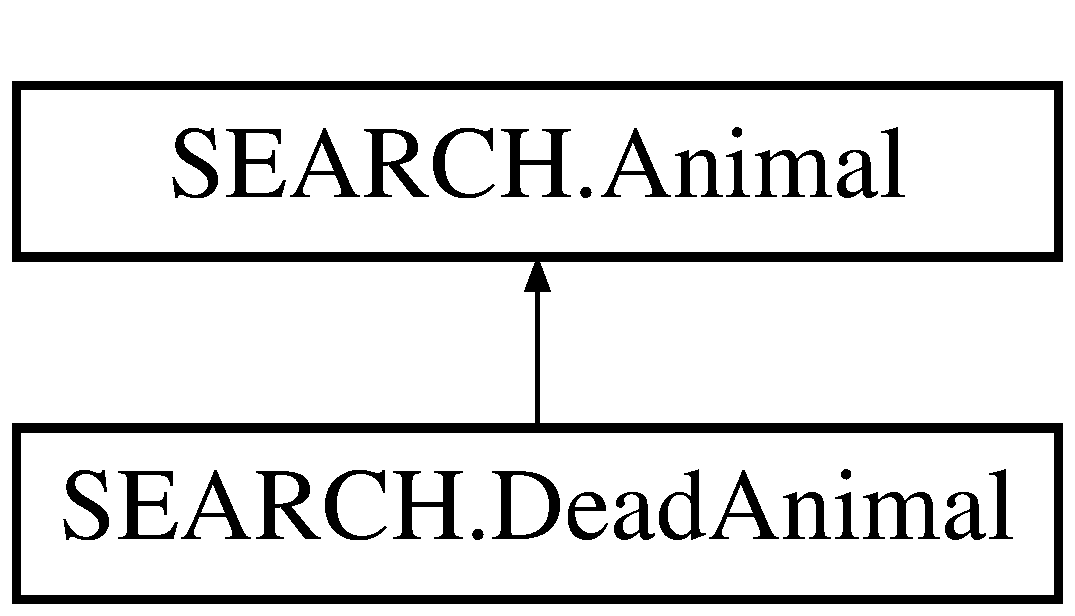
\includegraphics[height=2.000000cm]{class_s_e_a_r_c_h_1_1_dead_animal}
\end{center}
\end{figure}
\subsection*{Public Member Functions}
\begin{DoxyCompactItemize}
\item 
\hyperlink{class_s_e_a_r_c_h_1_1_dead_animal_a628e113b6148236806c8c26d15a3bf0a}{Dead\-Animal} ()
\item 
\hyperlink{class_s_e_a_r_c_h_1_1_dead_animal_a1dd08661985b38a5e453650a634ca1f8}{Dead\-Animal} (\hyperlink{class_s_e_a_r_c_h_1_1_animal}{Animal} a)
\item 
override void \hyperlink{class_s_e_a_r_c_h_1_1_dead_animal_a5a17ff4e63a89738621522de0658ae7b}{do\-Time\-Step} (\hyperlink{class_s_e_a_r_c_h_1_1_hourly_modifier}{Hourly\-Modifier} in\-H\-M, \hyperlink{class_s_e_a_r_c_h_1_1_daily_modifier}{Daily\-Modifier} in\-D\-M, Date\-Time curr\-Time, bool do\-Text\-Output, ref string status)
\end{DoxyCompactItemize}
\subsection*{Properties}
\begin{DoxyCompactItemize}
\item 
bool \hyperlink{class_s_e_a_r_c_h_1_1_dead_animal_a2f76897f9f6724ef178f20e5fae18fab}{Was\-Removed\-From\-Map}\hspace{0.3cm}{\ttfamily  \mbox{[}get, set\mbox{]}}
\item 
bool \hyperlink{class_s_e_a_r_c_h_1_1_dead_animal_a1bfa253d1b2f728f4b4682d0dbd0cc71}{Was\-Resident}\hspace{0.3cm}{\ttfamily  \mbox{[}get, set\mbox{]}}
\end{DoxyCompactItemize}
\subsection*{Additional Inherited Members}


\subsection{Detailed Description}
Summary description for Dead\-Disperser. 



\subsection{Constructor \& Destructor Documentation}
\hypertarget{class_s_e_a_r_c_h_1_1_dead_animal_a628e113b6148236806c8c26d15a3bf0a}{\index{S\-E\-A\-R\-C\-H\-::\-Dead\-Animal@{S\-E\-A\-R\-C\-H\-::\-Dead\-Animal}!Dead\-Animal@{Dead\-Animal}}
\index{Dead\-Animal@{Dead\-Animal}!SEARCH::DeadAnimal@{S\-E\-A\-R\-C\-H\-::\-Dead\-Animal}}
\subsubsection[{Dead\-Animal}]{\setlength{\rightskip}{0pt plus 5cm}S\-E\-A\-R\-C\-H.\-Dead\-Animal.\-Dead\-Animal (
\begin{DoxyParamCaption}
{}
\end{DoxyParamCaption}
)}}\label{class_s_e_a_r_c_h_1_1_dead_animal_a628e113b6148236806c8c26d15a3bf0a}
\hypertarget{class_s_e_a_r_c_h_1_1_dead_animal_a1dd08661985b38a5e453650a634ca1f8}{\index{S\-E\-A\-R\-C\-H\-::\-Dead\-Animal@{S\-E\-A\-R\-C\-H\-::\-Dead\-Animal}!Dead\-Animal@{Dead\-Animal}}
\index{Dead\-Animal@{Dead\-Animal}!SEARCH::DeadAnimal@{S\-E\-A\-R\-C\-H\-::\-Dead\-Animal}}
\subsubsection[{Dead\-Animal}]{\setlength{\rightskip}{0pt plus 5cm}S\-E\-A\-R\-C\-H.\-Dead\-Animal.\-Dead\-Animal (
\begin{DoxyParamCaption}
\item[{{\bf Animal}}]{a}
\end{DoxyParamCaption}
)}}\label{class_s_e_a_r_c_h_1_1_dead_animal_a1dd08661985b38a5e453650a634ca1f8}


\subsection{Member Function Documentation}
\hypertarget{class_s_e_a_r_c_h_1_1_dead_animal_a5a17ff4e63a89738621522de0658ae7b}{\index{S\-E\-A\-R\-C\-H\-::\-Dead\-Animal@{S\-E\-A\-R\-C\-H\-::\-Dead\-Animal}!do\-Time\-Step@{do\-Time\-Step}}
\index{do\-Time\-Step@{do\-Time\-Step}!SEARCH::DeadAnimal@{S\-E\-A\-R\-C\-H\-::\-Dead\-Animal}}
\subsubsection[{do\-Time\-Step}]{\setlength{\rightskip}{0pt plus 5cm}override void S\-E\-A\-R\-C\-H.\-Dead\-Animal.\-do\-Time\-Step (
\begin{DoxyParamCaption}
\item[{{\bf Hourly\-Modifier}}]{in\-H\-M, }
\item[{{\bf Daily\-Modifier}}]{in\-D\-M, }
\item[{Date\-Time}]{curr\-Time, }
\item[{bool}]{do\-Text\-Output, }
\item[{ref string}]{status}
\end{DoxyParamCaption}
)\hspace{0.3cm}{\ttfamily [virtual]}}}\label{class_s_e_a_r_c_h_1_1_dead_animal_a5a17ff4e63a89738621522de0658ae7b}


Reimplemented from \hyperlink{class_s_e_a_r_c_h_1_1_animal_ad805d6441c4c873121136b641c404f3a}{S\-E\-A\-R\-C\-H.\-Animal}.



\subsection{Property Documentation}
\hypertarget{class_s_e_a_r_c_h_1_1_dead_animal_a2f76897f9f6724ef178f20e5fae18fab}{\index{S\-E\-A\-R\-C\-H\-::\-Dead\-Animal@{S\-E\-A\-R\-C\-H\-::\-Dead\-Animal}!Was\-Removed\-From\-Map@{Was\-Removed\-From\-Map}}
\index{Was\-Removed\-From\-Map@{Was\-Removed\-From\-Map}!SEARCH::DeadAnimal@{S\-E\-A\-R\-C\-H\-::\-Dead\-Animal}}
\subsubsection[{Was\-Removed\-From\-Map}]{\setlength{\rightskip}{0pt plus 5cm}bool S\-E\-A\-R\-C\-H.\-Dead\-Animal.\-Was\-Removed\-From\-Map\hspace{0.3cm}{\ttfamily [get]}, {\ttfamily [set]}}}\label{class_s_e_a_r_c_h_1_1_dead_animal_a2f76897f9f6724ef178f20e5fae18fab}
\hypertarget{class_s_e_a_r_c_h_1_1_dead_animal_a1bfa253d1b2f728f4b4682d0dbd0cc71}{\index{S\-E\-A\-R\-C\-H\-::\-Dead\-Animal@{S\-E\-A\-R\-C\-H\-::\-Dead\-Animal}!Was\-Resident@{Was\-Resident}}
\index{Was\-Resident@{Was\-Resident}!SEARCH::DeadAnimal@{S\-E\-A\-R\-C\-H\-::\-Dead\-Animal}}
\subsubsection[{Was\-Resident}]{\setlength{\rightskip}{0pt plus 5cm}bool S\-E\-A\-R\-C\-H.\-Dead\-Animal.\-Was\-Resident\hspace{0.3cm}{\ttfamily [get]}, {\ttfamily [set]}}}\label{class_s_e_a_r_c_h_1_1_dead_animal_a1bfa253d1b2f728f4b4682d0dbd0cc71}


The documentation for this class was generated from the following file\-:\begin{DoxyCompactItemize}
\item 
Desktop/vlog4net\-A\-R\-C10\-\_\-64\-\_\-newhoming/\-Data\-Centric/\hyperlink{_dead_animal_8cs}{Dead\-Animal.\-cs}\end{DoxyCompactItemize}

\hypertarget{class_s_e_a_r_c_h_1_1_directed_mover}{\section{S\-E\-A\-R\-C\-H.\-Directed\-Mover Class Reference}
\label{class_s_e_a_r_c_h_1_1_directed_mover}\index{S\-E\-A\-R\-C\-H.\-Directed\-Mover@{S\-E\-A\-R\-C\-H.\-Directed\-Mover}}
}


 


Inheritance diagram for S\-E\-A\-R\-C\-H.\-Directed\-Mover\-:\begin{figure}[H]
\begin{center}
\leavevmode
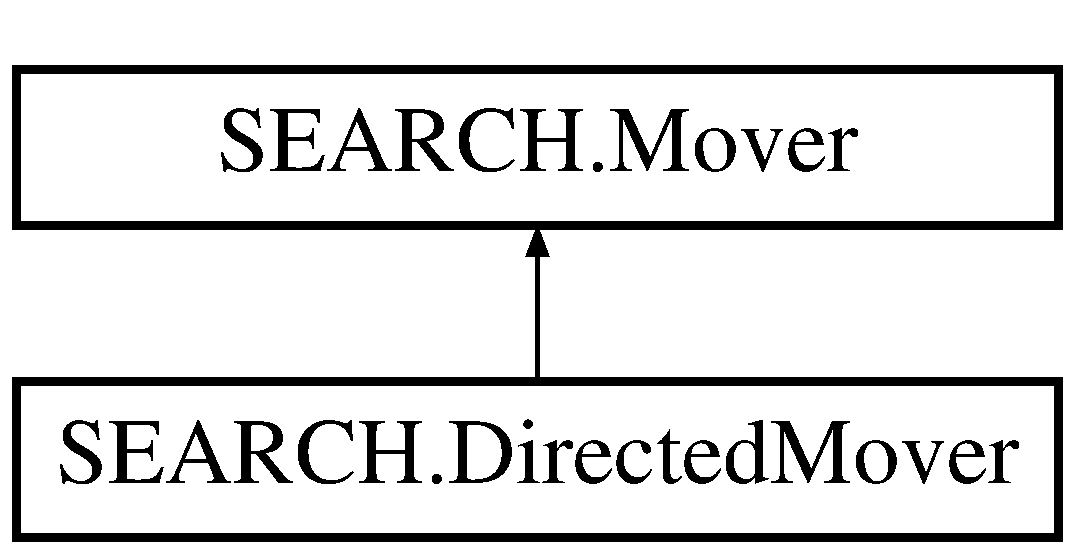
\includegraphics[height=2.000000cm]{class_s_e_a_r_c_h_1_1_directed_mover}
\end{center}
\end{figure}
\subsection*{Public Member Functions}
\begin{DoxyCompactItemize}
\item 
\hyperlink{class_s_e_a_r_c_h_1_1_directed_mover_a2cc387384dd525179200e71e50227527}{Directed\-Mover} ()
\item 
override double \hyperlink{class_s_e_a_r_c_h_1_1_directed_mover_ae103ba51cc5633f8f08a0f103869b446}{get\-Step\-Length} ()
\item 
override double \hyperlink{class_s_e_a_r_c_h_1_1_directed_mover_ac0ecb54d6c5b3c63d4959ce2ad5ba8b3}{get\-Turn\-Angle} (double turtosity)
\item 
override void \hyperlink{class_s_e_a_r_c_h_1_1_directed_mover_ac691f4b33dfc353cc0e5823649ecd874}{move} (ref double percent\-Time\-Step, \hyperlink{class_s_e_a_r_c_h_1_1_animal}{Animal} in\-A)
\end{DoxyCompactItemize}
\subsection*{Additional Inherited Members}


\subsection{Detailed Description}




\subsection{Constructor \& Destructor Documentation}
\hypertarget{class_s_e_a_r_c_h_1_1_directed_mover_a2cc387384dd525179200e71e50227527}{\index{S\-E\-A\-R\-C\-H\-::\-Directed\-Mover@{S\-E\-A\-R\-C\-H\-::\-Directed\-Mover}!Directed\-Mover@{Directed\-Mover}}
\index{Directed\-Mover@{Directed\-Mover}!SEARCH::DirectedMover@{S\-E\-A\-R\-C\-H\-::\-Directed\-Mover}}
\subsubsection[{Directed\-Mover}]{\setlength{\rightskip}{0pt plus 5cm}S\-E\-A\-R\-C\-H.\-Directed\-Mover.\-Directed\-Mover (
\begin{DoxyParamCaption}
{}
\end{DoxyParamCaption}
)}}\label{class_s_e_a_r_c_h_1_1_directed_mover_a2cc387384dd525179200e71e50227527}


\subsection{Member Function Documentation}
\hypertarget{class_s_e_a_r_c_h_1_1_directed_mover_ae103ba51cc5633f8f08a0f103869b446}{\index{S\-E\-A\-R\-C\-H\-::\-Directed\-Mover@{S\-E\-A\-R\-C\-H\-::\-Directed\-Mover}!get\-Step\-Length@{get\-Step\-Length}}
\index{get\-Step\-Length@{get\-Step\-Length}!SEARCH::DirectedMover@{S\-E\-A\-R\-C\-H\-::\-Directed\-Mover}}
\subsubsection[{get\-Step\-Length}]{\setlength{\rightskip}{0pt plus 5cm}override double S\-E\-A\-R\-C\-H.\-Directed\-Mover.\-get\-Step\-Length (
\begin{DoxyParamCaption}
{}
\end{DoxyParamCaption}
)\hspace{0.3cm}{\ttfamily [virtual]}}}\label{class_s_e_a_r_c_h_1_1_directed_mover_ae103ba51cc5633f8f08a0f103869b446}


Implements \hyperlink{class_s_e_a_r_c_h_1_1_mover_a3e547800bbc34492f4251adee70dbf02}{S\-E\-A\-R\-C\-H.\-Mover}.

\hypertarget{class_s_e_a_r_c_h_1_1_directed_mover_ac0ecb54d6c5b3c63d4959ce2ad5ba8b3}{\index{S\-E\-A\-R\-C\-H\-::\-Directed\-Mover@{S\-E\-A\-R\-C\-H\-::\-Directed\-Mover}!get\-Turn\-Angle@{get\-Turn\-Angle}}
\index{get\-Turn\-Angle@{get\-Turn\-Angle}!SEARCH::DirectedMover@{S\-E\-A\-R\-C\-H\-::\-Directed\-Mover}}
\subsubsection[{get\-Turn\-Angle}]{\setlength{\rightskip}{0pt plus 5cm}override double S\-E\-A\-R\-C\-H.\-Directed\-Mover.\-get\-Turn\-Angle (
\begin{DoxyParamCaption}
\item[{double}]{turtosity}
\end{DoxyParamCaption}
)\hspace{0.3cm}{\ttfamily [virtual]}}}\label{class_s_e_a_r_c_h_1_1_directed_mover_ac0ecb54d6c5b3c63d4959ce2ad5ba8b3}


Implements \hyperlink{class_s_e_a_r_c_h_1_1_mover_a879a44d5a0c57434375a69c8d8d00e35}{S\-E\-A\-R\-C\-H.\-Mover}.

\hypertarget{class_s_e_a_r_c_h_1_1_directed_mover_ac691f4b33dfc353cc0e5823649ecd874}{\index{S\-E\-A\-R\-C\-H\-::\-Directed\-Mover@{S\-E\-A\-R\-C\-H\-::\-Directed\-Mover}!move@{move}}
\index{move@{move}!SEARCH::DirectedMover@{S\-E\-A\-R\-C\-H\-::\-Directed\-Mover}}
\subsubsection[{move}]{\setlength{\rightskip}{0pt plus 5cm}override void S\-E\-A\-R\-C\-H.\-Directed\-Mover.\-move (
\begin{DoxyParamCaption}
\item[{ref double}]{percent\-Time\-Step, }
\item[{{\bf Animal}}]{in\-A}
\end{DoxyParamCaption}
)\hspace{0.3cm}{\ttfamily [virtual]}}}\label{class_s_e_a_r_c_h_1_1_directed_mover_ac691f4b33dfc353cc0e5823649ecd874}


Reimplemented from \hyperlink{class_s_e_a_r_c_h_1_1_mover_ab2dfc659f3817ea48d66ff4d7e464d1d}{S\-E\-A\-R\-C\-H.\-Mover}.



The documentation for this class was generated from the following file\-:\begin{DoxyCompactItemize}
\item 
Desktop/vlog4net\-A\-R\-C10\-\_\-64\-\_\-newhoming/\-Data\-Centric/\hyperlink{_directed_mover_8cs}{Directed\-Mover.\-cs}\end{DoxyCompactItemize}

\hypertarget{struct_s_e_a_r_c_h_1_1_duration}{\section{S\-E\-A\-R\-C\-H.\-Duration Struct Reference}
\label{struct_s_e_a_r_c_h_1_1_duration}\index{S\-E\-A\-R\-C\-H.\-Duration@{S\-E\-A\-R\-C\-H.\-Duration}}
}


Summary description for \hyperlink{struct_s_e_a_r_c_h_1_1_duration}{Duration}.  


\subsection*{Public Member Functions}
\begin{DoxyCompactItemize}
\item 
\hyperlink{struct_s_e_a_r_c_h_1_1_duration_a1a6b36c76b54c900adf43c5a82d43122}{Duration} (string in\-Type, double in\-Mean, double in\-S\-D)
\end{DoxyCompactItemize}
\subsection*{Properties}
\begin{DoxyCompactItemize}
\item 
double \hyperlink{struct_s_e_a_r_c_h_1_1_duration_aa3efd8fee940b36f5286f814bbce9f97}{Mean\-Amt}\hspace{0.3cm}{\ttfamily  \mbox{[}get, set\mbox{]}}
\item 
double \hyperlink{struct_s_e_a_r_c_h_1_1_duration_abd2fd1478a37e9f17c39062878d1805e}{Standard\-Deviation}\hspace{0.3cm}{\ttfamily  \mbox{[}get, set\mbox{]}}
\item 
string \hyperlink{struct_s_e_a_r_c_h_1_1_duration_ab51c7298f0c8181cd0f22d965090ca5a}{Type}\hspace{0.3cm}{\ttfamily  \mbox{[}get, set\mbox{]}}
\end{DoxyCompactItemize}


\subsection{Detailed Description}
Summary description for \hyperlink{struct_s_e_a_r_c_h_1_1_duration}{Duration}. 



\subsection{Constructor \& Destructor Documentation}
\hypertarget{struct_s_e_a_r_c_h_1_1_duration_a1a6b36c76b54c900adf43c5a82d43122}{\index{S\-E\-A\-R\-C\-H\-::\-Duration@{S\-E\-A\-R\-C\-H\-::\-Duration}!Duration@{Duration}}
\index{Duration@{Duration}!SEARCH::Duration@{S\-E\-A\-R\-C\-H\-::\-Duration}}
\subsubsection[{Duration}]{\setlength{\rightskip}{0pt plus 5cm}S\-E\-A\-R\-C\-H.\-Duration.\-Duration (
\begin{DoxyParamCaption}
\item[{string}]{in\-Type, }
\item[{double}]{in\-Mean, }
\item[{double}]{in\-S\-D}
\end{DoxyParamCaption}
)}}\label{struct_s_e_a_r_c_h_1_1_duration_a1a6b36c76b54c900adf43c5a82d43122}


\subsection{Property Documentation}
\hypertarget{struct_s_e_a_r_c_h_1_1_duration_aa3efd8fee940b36f5286f814bbce9f97}{\index{S\-E\-A\-R\-C\-H\-::\-Duration@{S\-E\-A\-R\-C\-H\-::\-Duration}!Mean\-Amt@{Mean\-Amt}}
\index{Mean\-Amt@{Mean\-Amt}!SEARCH::Duration@{S\-E\-A\-R\-C\-H\-::\-Duration}}
\subsubsection[{Mean\-Amt}]{\setlength{\rightskip}{0pt plus 5cm}double S\-E\-A\-R\-C\-H.\-Duration.\-Mean\-Amt\hspace{0.3cm}{\ttfamily [get]}, {\ttfamily [set]}}}\label{struct_s_e_a_r_c_h_1_1_duration_aa3efd8fee940b36f5286f814bbce9f97}
\hypertarget{struct_s_e_a_r_c_h_1_1_duration_abd2fd1478a37e9f17c39062878d1805e}{\index{S\-E\-A\-R\-C\-H\-::\-Duration@{S\-E\-A\-R\-C\-H\-::\-Duration}!Standard\-Deviation@{Standard\-Deviation}}
\index{Standard\-Deviation@{Standard\-Deviation}!SEARCH::Duration@{S\-E\-A\-R\-C\-H\-::\-Duration}}
\subsubsection[{Standard\-Deviation}]{\setlength{\rightskip}{0pt plus 5cm}double S\-E\-A\-R\-C\-H.\-Duration.\-Standard\-Deviation\hspace{0.3cm}{\ttfamily [get]}, {\ttfamily [set]}}}\label{struct_s_e_a_r_c_h_1_1_duration_abd2fd1478a37e9f17c39062878d1805e}
\hypertarget{struct_s_e_a_r_c_h_1_1_duration_ab51c7298f0c8181cd0f22d965090ca5a}{\index{S\-E\-A\-R\-C\-H\-::\-Duration@{S\-E\-A\-R\-C\-H\-::\-Duration}!Type@{Type}}
\index{Type@{Type}!SEARCH::Duration@{S\-E\-A\-R\-C\-H\-::\-Duration}}
\subsubsection[{Type}]{\setlength{\rightskip}{0pt plus 5cm}string S\-E\-A\-R\-C\-H.\-Duration.\-Type\hspace{0.3cm}{\ttfamily [get]}, {\ttfamily [set]}}}\label{struct_s_e_a_r_c_h_1_1_duration_ab51c7298f0c8181cd0f22d965090ca5a}


The documentation for this struct was generated from the following file\-:\begin{DoxyCompactItemize}
\item 
Desktop/vlog4net\-A\-R\-C10\-\_\-64\-\_\-newhoming/\-Data\-Centric/\hyperlink{_duration_8cs}{Duration.\-cs}\end{DoxyCompactItemize}

\hypertarget{class_s_e_a_r_c_h_1_1_eligible_home_site}{\section{S\-E\-A\-R\-C\-H.\-Eligible\-Home\-Site Class Reference}
\label{class_s_e_a_r_c_h_1_1_eligible_home_site}\index{S\-E\-A\-R\-C\-H.\-Eligible\-Home\-Site@{S\-E\-A\-R\-C\-H.\-Eligible\-Home\-Site}}
}


//holds the information about areas we have visited  


Inheritance diagram for S\-E\-A\-R\-C\-H.\-Eligible\-Home\-Site\-:\begin{figure}[H]
\begin{center}
\leavevmode
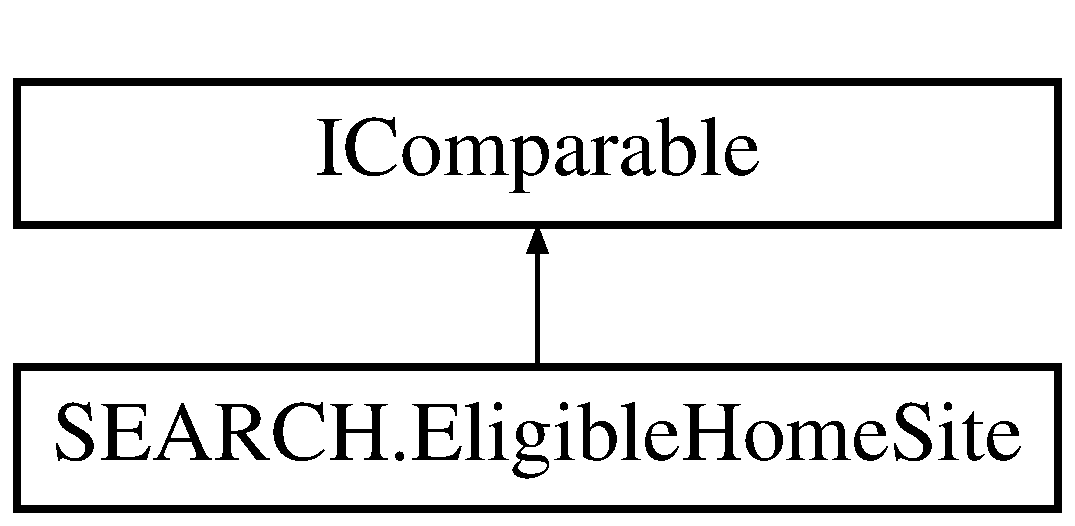
\includegraphics[height=2.000000cm]{class_s_e_a_r_c_h_1_1_eligible_home_site}
\end{center}
\end{figure}
\subsection*{Public Types}
\begin{DoxyCompactItemize}
\item 
enum \hyperlink{class_s_e_a_r_c_h_1_1_eligible_home_site_a072bac9d5910ce852eee90462451af81}{Sort\-Method} \{ \hyperlink{class_s_e_a_r_c_h_1_1_eligible_home_site_a072bac9d5910ce852eee90462451af81a0a38e7286ebbb560354992b3ce62be67}{Food} = 0, 
\hyperlink{class_s_e_a_r_c_h_1_1_eligible_home_site_a072bac9d5910ce852eee90462451af81a59ca88f7b0e80cdd9af330af600a9ff6}{Risk} = 1, 
\hyperlink{class_s_e_a_r_c_h_1_1_eligible_home_site_a072bac9d5910ce852eee90462451af81a021da1b20f73dc252361a54d80497ef3}{Rank} = 2, 
\hyperlink{class_s_e_a_r_c_h_1_1_eligible_home_site_a072bac9d5910ce852eee90462451af81a5c19fe9a1d52a0618136405798fc4f5f}{Dist} =3
 \}
\end{DoxyCompactItemize}
\subsection*{Public Member Functions}
\begin{DoxyCompactItemize}
\item 
\hyperlink{class_s_e_a_r_c_h_1_1_eligible_home_site_a60b41b254c87550d316d60faaa22054e}{Eligible\-Home\-Site} (double in\-Food, double in\-Risk, double in\-X, double in\-Y)
\item 
\hyperlink{class_s_e_a_r_c_h_1_1_eligible_home_site_a4a518d023ef6e226eccd4fe926d5995b}{Eligible\-Home\-Site} (double in\-X, double in\-Y)
\item 
\hyperlink{class_s_e_a_r_c_h_1_1_eligible_home_site_a53815d81eab83d7c7aeb1a81e19c1b68}{Eligible\-Home\-Site} (I\-Point in\-P)
\item 
\hyperlink{class_s_e_a_r_c_h_1_1_eligible_home_site_a520d4fd53cd96dc5647f6900382bc202}{Eligible\-Home\-Site} ()
\item 
int \hyperlink{class_s_e_a_r_c_h_1_1_eligible_home_site_a0733f24b55472257d0f31b596c8fba80}{Compare\-To} (object obj)
\end{DoxyCompactItemize}
\subsection*{Properties}
\begin{DoxyCompactItemize}
\item 
double \hyperlink{class_s_e_a_r_c_h_1_1_eligible_home_site_ad52a57d64d311a34d0ceb87c7c5c32ec}{Distance\-From\-Curr\-Location}\hspace{0.3cm}{\ttfamily  \mbox{[}get, set\mbox{]}}
\item 
bool \hyperlink{class_s_e_a_r_c_h_1_1_eligible_home_site_ae7ebeb841ca2a0eb5ae8a69bd1897522}{Suitable\-Site}\hspace{0.3cm}{\ttfamily  \mbox{[}get, set\mbox{]}}
\item 
double \hyperlink{class_s_e_a_r_c_h_1_1_eligible_home_site_a62de8ae874edce9d3786fa08e1e1eef3}{Rank}\hspace{0.3cm}{\ttfamily  \mbox{[}get, set\mbox{]}}
\item 
double \hyperlink{class_s_e_a_r_c_h_1_1_eligible_home_site_addea9a16468baa964161291bd5294617}{Food}\hspace{0.3cm}{\ttfamily  \mbox{[}get, set\mbox{]}}
\item 
double \hyperlink{class_s_e_a_r_c_h_1_1_eligible_home_site_af04910ec71a4c2692c0179e9c11e17f9}{Risk}\hspace{0.3cm}{\ttfamily  \mbox{[}get, set\mbox{]}}
\item 
double \hyperlink{class_s_e_a_r_c_h_1_1_eligible_home_site_a19b67a7f5c936dbea9a18f05fbb8ab3f}{X}\hspace{0.3cm}{\ttfamily  \mbox{[}get, set\mbox{]}}
\item 
double \hyperlink{class_s_e_a_r_c_h_1_1_eligible_home_site_a2f8dfc2534df3e398e135851dfc1d73f}{Y}\hspace{0.3cm}{\ttfamily  \mbox{[}get, set\mbox{]}}
\item 
static \hyperlink{class_s_e_a_r_c_h_1_1_eligible_home_site_a072bac9d5910ce852eee90462451af81}{Sort\-Method} \hyperlink{class_s_e_a_r_c_h_1_1_eligible_home_site_a294fc71059f845e2bdacbffa32005f81}{Sort\-Order}\hspace{0.3cm}{\ttfamily  \mbox{[}get, set\mbox{]}}
\end{DoxyCompactItemize}


\subsection{Detailed Description}
//holds the information about areas we have visited 



\subsection{Member Enumeration Documentation}
\hypertarget{class_s_e_a_r_c_h_1_1_eligible_home_site_a072bac9d5910ce852eee90462451af81}{\index{S\-E\-A\-R\-C\-H\-::\-Eligible\-Home\-Site@{S\-E\-A\-R\-C\-H\-::\-Eligible\-Home\-Site}!Sort\-Method@{Sort\-Method}}
\index{Sort\-Method@{Sort\-Method}!SEARCH::EligibleHomeSite@{S\-E\-A\-R\-C\-H\-::\-Eligible\-Home\-Site}}
\subsubsection[{Sort\-Method}]{\setlength{\rightskip}{0pt plus 5cm}enum {\bf S\-E\-A\-R\-C\-H.\-Eligible\-Home\-Site.\-Sort\-Method}}}\label{class_s_e_a_r_c_h_1_1_eligible_home_site_a072bac9d5910ce852eee90462451af81}
\begin{Desc}
\item[Enumerator]\par
\begin{description}
\index{Food@{Food}!S\-E\-A\-R\-C\-H\-::\-Eligible\-Home\-Site@{S\-E\-A\-R\-C\-H\-::\-Eligible\-Home\-Site}}\index{S\-E\-A\-R\-C\-H\-::\-Eligible\-Home\-Site@{S\-E\-A\-R\-C\-H\-::\-Eligible\-Home\-Site}!Food@{Food}}\item[{\em 
\hypertarget{class_s_e_a_r_c_h_1_1_eligible_home_site_a072bac9d5910ce852eee90462451af81a0a38e7286ebbb560354992b3ce62be67}{Food}\label{class_s_e_a_r_c_h_1_1_eligible_home_site_a072bac9d5910ce852eee90462451af81a0a38e7286ebbb560354992b3ce62be67}
}]\index{Risk@{Risk}!S\-E\-A\-R\-C\-H\-::\-Eligible\-Home\-Site@{S\-E\-A\-R\-C\-H\-::\-Eligible\-Home\-Site}}\index{S\-E\-A\-R\-C\-H\-::\-Eligible\-Home\-Site@{S\-E\-A\-R\-C\-H\-::\-Eligible\-Home\-Site}!Risk@{Risk}}\item[{\em 
\hypertarget{class_s_e_a_r_c_h_1_1_eligible_home_site_a072bac9d5910ce852eee90462451af81a59ca88f7b0e80cdd9af330af600a9ff6}{Risk}\label{class_s_e_a_r_c_h_1_1_eligible_home_site_a072bac9d5910ce852eee90462451af81a59ca88f7b0e80cdd9af330af600a9ff6}
}]\index{Rank@{Rank}!S\-E\-A\-R\-C\-H\-::\-Eligible\-Home\-Site@{S\-E\-A\-R\-C\-H\-::\-Eligible\-Home\-Site}}\index{S\-E\-A\-R\-C\-H\-::\-Eligible\-Home\-Site@{S\-E\-A\-R\-C\-H\-::\-Eligible\-Home\-Site}!Rank@{Rank}}\item[{\em 
\hypertarget{class_s_e_a_r_c_h_1_1_eligible_home_site_a072bac9d5910ce852eee90462451af81a021da1b20f73dc252361a54d80497ef3}{Rank}\label{class_s_e_a_r_c_h_1_1_eligible_home_site_a072bac9d5910ce852eee90462451af81a021da1b20f73dc252361a54d80497ef3}
}]\index{Dist@{Dist}!S\-E\-A\-R\-C\-H\-::\-Eligible\-Home\-Site@{S\-E\-A\-R\-C\-H\-::\-Eligible\-Home\-Site}}\index{S\-E\-A\-R\-C\-H\-::\-Eligible\-Home\-Site@{S\-E\-A\-R\-C\-H\-::\-Eligible\-Home\-Site}!Dist@{Dist}}\item[{\em 
\hypertarget{class_s_e_a_r_c_h_1_1_eligible_home_site_a072bac9d5910ce852eee90462451af81a5c19fe9a1d52a0618136405798fc4f5f}{Dist}\label{class_s_e_a_r_c_h_1_1_eligible_home_site_a072bac9d5910ce852eee90462451af81a5c19fe9a1d52a0618136405798fc4f5f}
}]\end{description}
\end{Desc}


\subsection{Constructor \& Destructor Documentation}
\hypertarget{class_s_e_a_r_c_h_1_1_eligible_home_site_a60b41b254c87550d316d60faaa22054e}{\index{S\-E\-A\-R\-C\-H\-::\-Eligible\-Home\-Site@{S\-E\-A\-R\-C\-H\-::\-Eligible\-Home\-Site}!Eligible\-Home\-Site@{Eligible\-Home\-Site}}
\index{Eligible\-Home\-Site@{Eligible\-Home\-Site}!SEARCH::EligibleHomeSite@{S\-E\-A\-R\-C\-H\-::\-Eligible\-Home\-Site}}
\subsubsection[{Eligible\-Home\-Site}]{\setlength{\rightskip}{0pt plus 5cm}S\-E\-A\-R\-C\-H.\-Eligible\-Home\-Site.\-Eligible\-Home\-Site (
\begin{DoxyParamCaption}
\item[{double}]{in\-Food, }
\item[{double}]{in\-Risk, }
\item[{double}]{in\-X, }
\item[{double}]{in\-Y}
\end{DoxyParamCaption}
)}}\label{class_s_e_a_r_c_h_1_1_eligible_home_site_a60b41b254c87550d316d60faaa22054e}
\hypertarget{class_s_e_a_r_c_h_1_1_eligible_home_site_a4a518d023ef6e226eccd4fe926d5995b}{\index{S\-E\-A\-R\-C\-H\-::\-Eligible\-Home\-Site@{S\-E\-A\-R\-C\-H\-::\-Eligible\-Home\-Site}!Eligible\-Home\-Site@{Eligible\-Home\-Site}}
\index{Eligible\-Home\-Site@{Eligible\-Home\-Site}!SEARCH::EligibleHomeSite@{S\-E\-A\-R\-C\-H\-::\-Eligible\-Home\-Site}}
\subsubsection[{Eligible\-Home\-Site}]{\setlength{\rightskip}{0pt plus 5cm}S\-E\-A\-R\-C\-H.\-Eligible\-Home\-Site.\-Eligible\-Home\-Site (
\begin{DoxyParamCaption}
\item[{double}]{in\-X, }
\item[{double}]{in\-Y}
\end{DoxyParamCaption}
)}}\label{class_s_e_a_r_c_h_1_1_eligible_home_site_a4a518d023ef6e226eccd4fe926d5995b}
\hypertarget{class_s_e_a_r_c_h_1_1_eligible_home_site_a53815d81eab83d7c7aeb1a81e19c1b68}{\index{S\-E\-A\-R\-C\-H\-::\-Eligible\-Home\-Site@{S\-E\-A\-R\-C\-H\-::\-Eligible\-Home\-Site}!Eligible\-Home\-Site@{Eligible\-Home\-Site}}
\index{Eligible\-Home\-Site@{Eligible\-Home\-Site}!SEARCH::EligibleHomeSite@{S\-E\-A\-R\-C\-H\-::\-Eligible\-Home\-Site}}
\subsubsection[{Eligible\-Home\-Site}]{\setlength{\rightskip}{0pt plus 5cm}S\-E\-A\-R\-C\-H.\-Eligible\-Home\-Site.\-Eligible\-Home\-Site (
\begin{DoxyParamCaption}
\item[{I\-Point}]{in\-P}
\end{DoxyParamCaption}
)}}\label{class_s_e_a_r_c_h_1_1_eligible_home_site_a53815d81eab83d7c7aeb1a81e19c1b68}
\hypertarget{class_s_e_a_r_c_h_1_1_eligible_home_site_a520d4fd53cd96dc5647f6900382bc202}{\index{S\-E\-A\-R\-C\-H\-::\-Eligible\-Home\-Site@{S\-E\-A\-R\-C\-H\-::\-Eligible\-Home\-Site}!Eligible\-Home\-Site@{Eligible\-Home\-Site}}
\index{Eligible\-Home\-Site@{Eligible\-Home\-Site}!SEARCH::EligibleHomeSite@{S\-E\-A\-R\-C\-H\-::\-Eligible\-Home\-Site}}
\subsubsection[{Eligible\-Home\-Site}]{\setlength{\rightskip}{0pt plus 5cm}S\-E\-A\-R\-C\-H.\-Eligible\-Home\-Site.\-Eligible\-Home\-Site (
\begin{DoxyParamCaption}
{}
\end{DoxyParamCaption}
)}}\label{class_s_e_a_r_c_h_1_1_eligible_home_site_a520d4fd53cd96dc5647f6900382bc202}


\subsection{Member Function Documentation}
\hypertarget{class_s_e_a_r_c_h_1_1_eligible_home_site_a0733f24b55472257d0f31b596c8fba80}{\index{S\-E\-A\-R\-C\-H\-::\-Eligible\-Home\-Site@{S\-E\-A\-R\-C\-H\-::\-Eligible\-Home\-Site}!Compare\-To@{Compare\-To}}
\index{Compare\-To@{Compare\-To}!SEARCH::EligibleHomeSite@{S\-E\-A\-R\-C\-H\-::\-Eligible\-Home\-Site}}
\subsubsection[{Compare\-To}]{\setlength{\rightskip}{0pt plus 5cm}int S\-E\-A\-R\-C\-H.\-Eligible\-Home\-Site.\-Compare\-To (
\begin{DoxyParamCaption}
\item[{object}]{obj}
\end{DoxyParamCaption}
)}}\label{class_s_e_a_r_c_h_1_1_eligible_home_site_a0733f24b55472257d0f31b596c8fba80}


\subsection{Property Documentation}
\hypertarget{class_s_e_a_r_c_h_1_1_eligible_home_site_ad52a57d64d311a34d0ceb87c7c5c32ec}{\index{S\-E\-A\-R\-C\-H\-::\-Eligible\-Home\-Site@{S\-E\-A\-R\-C\-H\-::\-Eligible\-Home\-Site}!Distance\-From\-Curr\-Location@{Distance\-From\-Curr\-Location}}
\index{Distance\-From\-Curr\-Location@{Distance\-From\-Curr\-Location}!SEARCH::EligibleHomeSite@{S\-E\-A\-R\-C\-H\-::\-Eligible\-Home\-Site}}
\subsubsection[{Distance\-From\-Curr\-Location}]{\setlength{\rightskip}{0pt plus 5cm}double S\-E\-A\-R\-C\-H.\-Eligible\-Home\-Site.\-Distance\-From\-Curr\-Location\hspace{0.3cm}{\ttfamily [get]}, {\ttfamily [set]}}}\label{class_s_e_a_r_c_h_1_1_eligible_home_site_ad52a57d64d311a34d0ceb87c7c5c32ec}
\hypertarget{class_s_e_a_r_c_h_1_1_eligible_home_site_addea9a16468baa964161291bd5294617}{\index{S\-E\-A\-R\-C\-H\-::\-Eligible\-Home\-Site@{S\-E\-A\-R\-C\-H\-::\-Eligible\-Home\-Site}!Food@{Food}}
\index{Food@{Food}!SEARCH::EligibleHomeSite@{S\-E\-A\-R\-C\-H\-::\-Eligible\-Home\-Site}}
\subsubsection[{Food}]{\setlength{\rightskip}{0pt plus 5cm}double S\-E\-A\-R\-C\-H.\-Eligible\-Home\-Site.\-Food\hspace{0.3cm}{\ttfamily [get]}, {\ttfamily [set]}}}\label{class_s_e_a_r_c_h_1_1_eligible_home_site_addea9a16468baa964161291bd5294617}
\hypertarget{class_s_e_a_r_c_h_1_1_eligible_home_site_a62de8ae874edce9d3786fa08e1e1eef3}{\index{S\-E\-A\-R\-C\-H\-::\-Eligible\-Home\-Site@{S\-E\-A\-R\-C\-H\-::\-Eligible\-Home\-Site}!Rank@{Rank}}
\index{Rank@{Rank}!SEARCH::EligibleHomeSite@{S\-E\-A\-R\-C\-H\-::\-Eligible\-Home\-Site}}
\subsubsection[{Rank}]{\setlength{\rightskip}{0pt plus 5cm}double S\-E\-A\-R\-C\-H.\-Eligible\-Home\-Site.\-Rank\hspace{0.3cm}{\ttfamily [get]}, {\ttfamily [set]}}}\label{class_s_e_a_r_c_h_1_1_eligible_home_site_a62de8ae874edce9d3786fa08e1e1eef3}
\hypertarget{class_s_e_a_r_c_h_1_1_eligible_home_site_af04910ec71a4c2692c0179e9c11e17f9}{\index{S\-E\-A\-R\-C\-H\-::\-Eligible\-Home\-Site@{S\-E\-A\-R\-C\-H\-::\-Eligible\-Home\-Site}!Risk@{Risk}}
\index{Risk@{Risk}!SEARCH::EligibleHomeSite@{S\-E\-A\-R\-C\-H\-::\-Eligible\-Home\-Site}}
\subsubsection[{Risk}]{\setlength{\rightskip}{0pt plus 5cm}double S\-E\-A\-R\-C\-H.\-Eligible\-Home\-Site.\-Risk\hspace{0.3cm}{\ttfamily [get]}, {\ttfamily [set]}}}\label{class_s_e_a_r_c_h_1_1_eligible_home_site_af04910ec71a4c2692c0179e9c11e17f9}
\hypertarget{class_s_e_a_r_c_h_1_1_eligible_home_site_a294fc71059f845e2bdacbffa32005f81}{\index{S\-E\-A\-R\-C\-H\-::\-Eligible\-Home\-Site@{S\-E\-A\-R\-C\-H\-::\-Eligible\-Home\-Site}!Sort\-Order@{Sort\-Order}}
\index{Sort\-Order@{Sort\-Order}!SEARCH::EligibleHomeSite@{S\-E\-A\-R\-C\-H\-::\-Eligible\-Home\-Site}}
\subsubsection[{Sort\-Order}]{\setlength{\rightskip}{0pt plus 5cm}{\bf Sort\-Method} S\-E\-A\-R\-C\-H.\-Eligible\-Home\-Site.\-Sort\-Order\hspace{0.3cm}{\ttfamily [static]}, {\ttfamily [get]}, {\ttfamily [set]}}}\label{class_s_e_a_r_c_h_1_1_eligible_home_site_a294fc71059f845e2bdacbffa32005f81}
\hypertarget{class_s_e_a_r_c_h_1_1_eligible_home_site_ae7ebeb841ca2a0eb5ae8a69bd1897522}{\index{S\-E\-A\-R\-C\-H\-::\-Eligible\-Home\-Site@{S\-E\-A\-R\-C\-H\-::\-Eligible\-Home\-Site}!Suitable\-Site@{Suitable\-Site}}
\index{Suitable\-Site@{Suitable\-Site}!SEARCH::EligibleHomeSite@{S\-E\-A\-R\-C\-H\-::\-Eligible\-Home\-Site}}
\subsubsection[{Suitable\-Site}]{\setlength{\rightskip}{0pt plus 5cm}bool S\-E\-A\-R\-C\-H.\-Eligible\-Home\-Site.\-Suitable\-Site\hspace{0.3cm}{\ttfamily [get]}, {\ttfamily [set]}}}\label{class_s_e_a_r_c_h_1_1_eligible_home_site_ae7ebeb841ca2a0eb5ae8a69bd1897522}
\hypertarget{class_s_e_a_r_c_h_1_1_eligible_home_site_a19b67a7f5c936dbea9a18f05fbb8ab3f}{\index{S\-E\-A\-R\-C\-H\-::\-Eligible\-Home\-Site@{S\-E\-A\-R\-C\-H\-::\-Eligible\-Home\-Site}!X@{X}}
\index{X@{X}!SEARCH::EligibleHomeSite@{S\-E\-A\-R\-C\-H\-::\-Eligible\-Home\-Site}}
\subsubsection[{X}]{\setlength{\rightskip}{0pt plus 5cm}double S\-E\-A\-R\-C\-H.\-Eligible\-Home\-Site.\-X\hspace{0.3cm}{\ttfamily [get]}, {\ttfamily [set]}}}\label{class_s_e_a_r_c_h_1_1_eligible_home_site_a19b67a7f5c936dbea9a18f05fbb8ab3f}
\hypertarget{class_s_e_a_r_c_h_1_1_eligible_home_site_a2f8dfc2534df3e398e135851dfc1d73f}{\index{S\-E\-A\-R\-C\-H\-::\-Eligible\-Home\-Site@{S\-E\-A\-R\-C\-H\-::\-Eligible\-Home\-Site}!Y@{Y}}
\index{Y@{Y}!SEARCH::EligibleHomeSite@{S\-E\-A\-R\-C\-H\-::\-Eligible\-Home\-Site}}
\subsubsection[{Y}]{\setlength{\rightskip}{0pt plus 5cm}double S\-E\-A\-R\-C\-H.\-Eligible\-Home\-Site.\-Y\hspace{0.3cm}{\ttfamily [get]}, {\ttfamily [set]}}}\label{class_s_e_a_r_c_h_1_1_eligible_home_site_a2f8dfc2534df3e398e135851dfc1d73f}


The documentation for this class was generated from the following file\-:\begin{DoxyCompactItemize}
\item 
Desktop/vlog4net\-A\-R\-C10\-\_\-64\-\_\-newhoming/\-Data\-Centric/\hyperlink{_eligible_home_site_8cs}{Eligible\-Home\-Site.\-cs}\end{DoxyCompactItemize}

\hypertarget{class_s_e_a_r_c_h_1_1_eligible_home_sites}{\section{S\-E\-A\-R\-C\-H.\-Eligible\-Home\-Sites Class Reference}
\label{class_s_e_a_r_c_h_1_1_eligible_home_sites}\index{S\-E\-A\-R\-C\-H.\-Eligible\-Home\-Sites@{S\-E\-A\-R\-C\-H.\-Eligible\-Home\-Sites}}
}


Summary description for \hyperlink{class_s_e_a_r_c_h_1_1_eligible_home_sites}{Eligible\-Home\-Sites}.  


\subsection*{Public Member Functions}
\begin{DoxyCompactItemize}
\item 
\hyperlink{class_s_e_a_r_c_h_1_1_eligible_home_sites_adbe8759b791c2e1003c786eede9bc644}{Eligible\-Home\-Sites} ()
\item 
void \hyperlink{class_s_e_a_r_c_h_1_1_eligible_home_sites_a1f11e669975303d7d2d5eaa70f7eaeb5}{add\-Site} (\hyperlink{class_s_e_a_r_c_h_1_1_eligible_home_site}{Eligible\-Home\-Site} in\-Site)
\item 
\hyperlink{class_s_e_a_r_c_h_1_1_eligible_home_site}{Eligible\-Home\-Site} \hyperlink{class_s_e_a_r_c_h_1_1_eligible_home_sites_a8992ff7ed00648e1b5198c93740e863d}{get\-First\-Suitable\-Site} ()
\item 
List$<$ I\-Point $>$ \hyperlink{class_s_e_a_r_c_h_1_1_eligible_home_sites_a355adc97933b85c303ad5529c0858c45}{get\-Points} ()
\item 
List$<$ \hyperlink{class_s_e_a_r_c_h_1_1_eligible_home_site}{Eligible\-Home\-Site} $>$ \hyperlink{class_s_e_a_r_c_h_1_1_eligible_home_sites_a6312de00ba952bf68fa09bc2f6b7c977}{get\-Qualified\-Sites} ()
\item 
\hyperlink{class_s_e_a_r_c_h_1_1_eligible_home_site}{Eligible\-Home\-Site} \hyperlink{class_s_e_a_r_c_h_1_1_eligible_home_sites_a4e202ce1ba8f052e884aed2b2122b332}{get\-Site} (int index)
\item 
void \hyperlink{class_s_e_a_r_c_h_1_1_eligible_home_sites_adae2d4a814ad7417e4a67068dbf0e69a}{Remove\-Site} (I\-Point in\-Point)
\item 
void \hyperlink{class_s_e_a_r_c_h_1_1_eligible_home_sites_a205ba5d8fbc8653b23344bd5a4d7a968}{set\-Combo\-Rank} (double distance\-Factor)
\item 
void \hyperlink{class_s_e_a_r_c_h_1_1_eligible_home_sites_a071e1c850cec41ec37a0a18c3ca949b4}{set\-Food\-Rank} (double distance\-Factor)
\item 
void \hyperlink{class_s_e_a_r_c_h_1_1_eligible_home_sites_a2c2d128066e76e1596bca446d9c08e7b}{set\-Ranges} (double in\-Double)
\item 
void \hyperlink{class_s_e_a_r_c_h_1_1_eligible_home_sites_a619f830931bf95e62ccc70fe48fd9f38}{Set\-Ranges} (double in\-Value, List$<$ \hyperlink{class_s_e_a_r_c_h_1_1_eligible_home_site}{Eligible\-Home\-Site} $>$ in\-Sites)
\item 
void \hyperlink{class_s_e_a_r_c_h_1_1_eligible_home_sites_a5c532ee2682a6a672f5c17ad64c45de5}{set\-Risk\-Rank} (double distance\-Factor)
\item 
void \hyperlink{class_s_e_a_r_c_h_1_1_eligible_home_sites_ae0f01cf21b8d5cdbc3c9f2e5b3b4e160}{Sort\-Sites} ()
\end{DoxyCompactItemize}
\subsection*{Properties}
\begin{DoxyCompactItemize}
\item 
List$<$ \hyperlink{class_s_e_a_r_c_h_1_1_eligible_home_site}{Eligible\-Home\-Site} $>$ \hyperlink{class_s_e_a_r_c_h_1_1_eligible_home_sites_a684dbb1fed6dc8c5904d4679f2fc5d53}{My\-Sites}\hspace{0.3cm}{\ttfamily  \mbox{[}get, set\mbox{]}}
\item 
int \hyperlink{class_s_e_a_r_c_h_1_1_eligible_home_sites_ab66a08f1ef23f2a5799a1dd4fefaf1bf}{Site\-Count}\hspace{0.3cm}{\ttfamily  \mbox{[}get\mbox{]}}
\end{DoxyCompactItemize}


\subsection{Detailed Description}
Summary description for \hyperlink{class_s_e_a_r_c_h_1_1_eligible_home_sites}{Eligible\-Home\-Sites}. 



\subsection{Constructor \& Destructor Documentation}
\hypertarget{class_s_e_a_r_c_h_1_1_eligible_home_sites_adbe8759b791c2e1003c786eede9bc644}{\index{S\-E\-A\-R\-C\-H\-::\-Eligible\-Home\-Sites@{S\-E\-A\-R\-C\-H\-::\-Eligible\-Home\-Sites}!Eligible\-Home\-Sites@{Eligible\-Home\-Sites}}
\index{Eligible\-Home\-Sites@{Eligible\-Home\-Sites}!SEARCH::EligibleHomeSites@{S\-E\-A\-R\-C\-H\-::\-Eligible\-Home\-Sites}}
\subsubsection[{Eligible\-Home\-Sites}]{\setlength{\rightskip}{0pt plus 5cm}S\-E\-A\-R\-C\-H.\-Eligible\-Home\-Sites.\-Eligible\-Home\-Sites (
\begin{DoxyParamCaption}
{}
\end{DoxyParamCaption}
)}}\label{class_s_e_a_r_c_h_1_1_eligible_home_sites_adbe8759b791c2e1003c786eede9bc644}


\subsection{Member Function Documentation}
\hypertarget{class_s_e_a_r_c_h_1_1_eligible_home_sites_a1f11e669975303d7d2d5eaa70f7eaeb5}{\index{S\-E\-A\-R\-C\-H\-::\-Eligible\-Home\-Sites@{S\-E\-A\-R\-C\-H\-::\-Eligible\-Home\-Sites}!add\-Site@{add\-Site}}
\index{add\-Site@{add\-Site}!SEARCH::EligibleHomeSites@{S\-E\-A\-R\-C\-H\-::\-Eligible\-Home\-Sites}}
\subsubsection[{add\-Site}]{\setlength{\rightskip}{0pt plus 5cm}void S\-E\-A\-R\-C\-H.\-Eligible\-Home\-Sites.\-add\-Site (
\begin{DoxyParamCaption}
\item[{{\bf Eligible\-Home\-Site}}]{in\-Site}
\end{DoxyParamCaption}
)}}\label{class_s_e_a_r_c_h_1_1_eligible_home_sites_a1f11e669975303d7d2d5eaa70f7eaeb5}
\hypertarget{class_s_e_a_r_c_h_1_1_eligible_home_sites_a8992ff7ed00648e1b5198c93740e863d}{\index{S\-E\-A\-R\-C\-H\-::\-Eligible\-Home\-Sites@{S\-E\-A\-R\-C\-H\-::\-Eligible\-Home\-Sites}!get\-First\-Suitable\-Site@{get\-First\-Suitable\-Site}}
\index{get\-First\-Suitable\-Site@{get\-First\-Suitable\-Site}!SEARCH::EligibleHomeSites@{S\-E\-A\-R\-C\-H\-::\-Eligible\-Home\-Sites}}
\subsubsection[{get\-First\-Suitable\-Site}]{\setlength{\rightskip}{0pt plus 5cm}{\bf Eligible\-Home\-Site} S\-E\-A\-R\-C\-H.\-Eligible\-Home\-Sites.\-get\-First\-Suitable\-Site (
\begin{DoxyParamCaption}
{}
\end{DoxyParamCaption}
)}}\label{class_s_e_a_r_c_h_1_1_eligible_home_sites_a8992ff7ed00648e1b5198c93740e863d}
\hypertarget{class_s_e_a_r_c_h_1_1_eligible_home_sites_a355adc97933b85c303ad5529c0858c45}{\index{S\-E\-A\-R\-C\-H\-::\-Eligible\-Home\-Sites@{S\-E\-A\-R\-C\-H\-::\-Eligible\-Home\-Sites}!get\-Points@{get\-Points}}
\index{get\-Points@{get\-Points}!SEARCH::EligibleHomeSites@{S\-E\-A\-R\-C\-H\-::\-Eligible\-Home\-Sites}}
\subsubsection[{get\-Points}]{\setlength{\rightskip}{0pt plus 5cm}List$<$I\-Point$>$ S\-E\-A\-R\-C\-H.\-Eligible\-Home\-Sites.\-get\-Points (
\begin{DoxyParamCaption}
{}
\end{DoxyParamCaption}
)}}\label{class_s_e_a_r_c_h_1_1_eligible_home_sites_a355adc97933b85c303ad5529c0858c45}
\hypertarget{class_s_e_a_r_c_h_1_1_eligible_home_sites_a6312de00ba952bf68fa09bc2f6b7c977}{\index{S\-E\-A\-R\-C\-H\-::\-Eligible\-Home\-Sites@{S\-E\-A\-R\-C\-H\-::\-Eligible\-Home\-Sites}!get\-Qualified\-Sites@{get\-Qualified\-Sites}}
\index{get\-Qualified\-Sites@{get\-Qualified\-Sites}!SEARCH::EligibleHomeSites@{S\-E\-A\-R\-C\-H\-::\-Eligible\-Home\-Sites}}
\subsubsection[{get\-Qualified\-Sites}]{\setlength{\rightskip}{0pt plus 5cm}List$<${\bf Eligible\-Home\-Site}$>$ S\-E\-A\-R\-C\-H.\-Eligible\-Home\-Sites.\-get\-Qualified\-Sites (
\begin{DoxyParamCaption}
{}
\end{DoxyParamCaption}
)}}\label{class_s_e_a_r_c_h_1_1_eligible_home_sites_a6312de00ba952bf68fa09bc2f6b7c977}
\hypertarget{class_s_e_a_r_c_h_1_1_eligible_home_sites_a4e202ce1ba8f052e884aed2b2122b332}{\index{S\-E\-A\-R\-C\-H\-::\-Eligible\-Home\-Sites@{S\-E\-A\-R\-C\-H\-::\-Eligible\-Home\-Sites}!get\-Site@{get\-Site}}
\index{get\-Site@{get\-Site}!SEARCH::EligibleHomeSites@{S\-E\-A\-R\-C\-H\-::\-Eligible\-Home\-Sites}}
\subsubsection[{get\-Site}]{\setlength{\rightskip}{0pt plus 5cm}{\bf Eligible\-Home\-Site} S\-E\-A\-R\-C\-H.\-Eligible\-Home\-Sites.\-get\-Site (
\begin{DoxyParamCaption}
\item[{int}]{index}
\end{DoxyParamCaption}
)}}\label{class_s_e_a_r_c_h_1_1_eligible_home_sites_a4e202ce1ba8f052e884aed2b2122b332}
\hypertarget{class_s_e_a_r_c_h_1_1_eligible_home_sites_adae2d4a814ad7417e4a67068dbf0e69a}{\index{S\-E\-A\-R\-C\-H\-::\-Eligible\-Home\-Sites@{S\-E\-A\-R\-C\-H\-::\-Eligible\-Home\-Sites}!Remove\-Site@{Remove\-Site}}
\index{Remove\-Site@{Remove\-Site}!SEARCH::EligibleHomeSites@{S\-E\-A\-R\-C\-H\-::\-Eligible\-Home\-Sites}}
\subsubsection[{Remove\-Site}]{\setlength{\rightskip}{0pt plus 5cm}void S\-E\-A\-R\-C\-H.\-Eligible\-Home\-Sites.\-Remove\-Site (
\begin{DoxyParamCaption}
\item[{I\-Point}]{in\-Point}
\end{DoxyParamCaption}
)}}\label{class_s_e_a_r_c_h_1_1_eligible_home_sites_adae2d4a814ad7417e4a67068dbf0e69a}
\hypertarget{class_s_e_a_r_c_h_1_1_eligible_home_sites_a205ba5d8fbc8653b23344bd5a4d7a968}{\index{S\-E\-A\-R\-C\-H\-::\-Eligible\-Home\-Sites@{S\-E\-A\-R\-C\-H\-::\-Eligible\-Home\-Sites}!set\-Combo\-Rank@{set\-Combo\-Rank}}
\index{set\-Combo\-Rank@{set\-Combo\-Rank}!SEARCH::EligibleHomeSites@{S\-E\-A\-R\-C\-H\-::\-Eligible\-Home\-Sites}}
\subsubsection[{set\-Combo\-Rank}]{\setlength{\rightskip}{0pt plus 5cm}void S\-E\-A\-R\-C\-H.\-Eligible\-Home\-Sites.\-set\-Combo\-Rank (
\begin{DoxyParamCaption}
\item[{double}]{distance\-Factor}
\end{DoxyParamCaption}
)}}\label{class_s_e_a_r_c_h_1_1_eligible_home_sites_a205ba5d8fbc8653b23344bd5a4d7a968}
\hypertarget{class_s_e_a_r_c_h_1_1_eligible_home_sites_a071e1c850cec41ec37a0a18c3ca949b4}{\index{S\-E\-A\-R\-C\-H\-::\-Eligible\-Home\-Sites@{S\-E\-A\-R\-C\-H\-::\-Eligible\-Home\-Sites}!set\-Food\-Rank@{set\-Food\-Rank}}
\index{set\-Food\-Rank@{set\-Food\-Rank}!SEARCH::EligibleHomeSites@{S\-E\-A\-R\-C\-H\-::\-Eligible\-Home\-Sites}}
\subsubsection[{set\-Food\-Rank}]{\setlength{\rightskip}{0pt plus 5cm}void S\-E\-A\-R\-C\-H.\-Eligible\-Home\-Sites.\-set\-Food\-Rank (
\begin{DoxyParamCaption}
\item[{double}]{distance\-Factor}
\end{DoxyParamCaption}
)}}\label{class_s_e_a_r_c_h_1_1_eligible_home_sites_a071e1c850cec41ec37a0a18c3ca949b4}
\hypertarget{class_s_e_a_r_c_h_1_1_eligible_home_sites_a2c2d128066e76e1596bca446d9c08e7b}{\index{S\-E\-A\-R\-C\-H\-::\-Eligible\-Home\-Sites@{S\-E\-A\-R\-C\-H\-::\-Eligible\-Home\-Sites}!set\-Ranges@{set\-Ranges}}
\index{set\-Ranges@{set\-Ranges}!SEARCH::EligibleHomeSites@{S\-E\-A\-R\-C\-H\-::\-Eligible\-Home\-Sites}}
\subsubsection[{set\-Ranges}]{\setlength{\rightskip}{0pt plus 5cm}void S\-E\-A\-R\-C\-H.\-Eligible\-Home\-Sites.\-set\-Ranges (
\begin{DoxyParamCaption}
\item[{double}]{in\-Double}
\end{DoxyParamCaption}
)}}\label{class_s_e_a_r_c_h_1_1_eligible_home_sites_a2c2d128066e76e1596bca446d9c08e7b}
\hypertarget{class_s_e_a_r_c_h_1_1_eligible_home_sites_a619f830931bf95e62ccc70fe48fd9f38}{\index{S\-E\-A\-R\-C\-H\-::\-Eligible\-Home\-Sites@{S\-E\-A\-R\-C\-H\-::\-Eligible\-Home\-Sites}!Set\-Ranges@{Set\-Ranges}}
\index{Set\-Ranges@{Set\-Ranges}!SEARCH::EligibleHomeSites@{S\-E\-A\-R\-C\-H\-::\-Eligible\-Home\-Sites}}
\subsubsection[{Set\-Ranges}]{\setlength{\rightskip}{0pt plus 5cm}void S\-E\-A\-R\-C\-H.\-Eligible\-Home\-Sites.\-Set\-Ranges (
\begin{DoxyParamCaption}
\item[{double}]{in\-Value, }
\item[{List$<$ {\bf Eligible\-Home\-Site} $>$}]{in\-Sites}
\end{DoxyParamCaption}
)}}\label{class_s_e_a_r_c_h_1_1_eligible_home_sites_a619f830931bf95e62ccc70fe48fd9f38}
\hypertarget{class_s_e_a_r_c_h_1_1_eligible_home_sites_a5c532ee2682a6a672f5c17ad64c45de5}{\index{S\-E\-A\-R\-C\-H\-::\-Eligible\-Home\-Sites@{S\-E\-A\-R\-C\-H\-::\-Eligible\-Home\-Sites}!set\-Risk\-Rank@{set\-Risk\-Rank}}
\index{set\-Risk\-Rank@{set\-Risk\-Rank}!SEARCH::EligibleHomeSites@{S\-E\-A\-R\-C\-H\-::\-Eligible\-Home\-Sites}}
\subsubsection[{set\-Risk\-Rank}]{\setlength{\rightskip}{0pt plus 5cm}void S\-E\-A\-R\-C\-H.\-Eligible\-Home\-Sites.\-set\-Risk\-Rank (
\begin{DoxyParamCaption}
\item[{double}]{distance\-Factor}
\end{DoxyParamCaption}
)}}\label{class_s_e_a_r_c_h_1_1_eligible_home_sites_a5c532ee2682a6a672f5c17ad64c45de5}
\hypertarget{class_s_e_a_r_c_h_1_1_eligible_home_sites_ae0f01cf21b8d5cdbc3c9f2e5b3b4e160}{\index{S\-E\-A\-R\-C\-H\-::\-Eligible\-Home\-Sites@{S\-E\-A\-R\-C\-H\-::\-Eligible\-Home\-Sites}!Sort\-Sites@{Sort\-Sites}}
\index{Sort\-Sites@{Sort\-Sites}!SEARCH::EligibleHomeSites@{S\-E\-A\-R\-C\-H\-::\-Eligible\-Home\-Sites}}
\subsubsection[{Sort\-Sites}]{\setlength{\rightskip}{0pt plus 5cm}void S\-E\-A\-R\-C\-H.\-Eligible\-Home\-Sites.\-Sort\-Sites (
\begin{DoxyParamCaption}
{}
\end{DoxyParamCaption}
)}}\label{class_s_e_a_r_c_h_1_1_eligible_home_sites_ae0f01cf21b8d5cdbc3c9f2e5b3b4e160}


\subsection{Property Documentation}
\hypertarget{class_s_e_a_r_c_h_1_1_eligible_home_sites_a684dbb1fed6dc8c5904d4679f2fc5d53}{\index{S\-E\-A\-R\-C\-H\-::\-Eligible\-Home\-Sites@{S\-E\-A\-R\-C\-H\-::\-Eligible\-Home\-Sites}!My\-Sites@{My\-Sites}}
\index{My\-Sites@{My\-Sites}!SEARCH::EligibleHomeSites@{S\-E\-A\-R\-C\-H\-::\-Eligible\-Home\-Sites}}
\subsubsection[{My\-Sites}]{\setlength{\rightskip}{0pt plus 5cm}List$<${\bf Eligible\-Home\-Site}$>$ S\-E\-A\-R\-C\-H.\-Eligible\-Home\-Sites.\-My\-Sites\hspace{0.3cm}{\ttfamily [get]}, {\ttfamily [set]}}}\label{class_s_e_a_r_c_h_1_1_eligible_home_sites_a684dbb1fed6dc8c5904d4679f2fc5d53}
\hypertarget{class_s_e_a_r_c_h_1_1_eligible_home_sites_ab66a08f1ef23f2a5799a1dd4fefaf1bf}{\index{S\-E\-A\-R\-C\-H\-::\-Eligible\-Home\-Sites@{S\-E\-A\-R\-C\-H\-::\-Eligible\-Home\-Sites}!Site\-Count@{Site\-Count}}
\index{Site\-Count@{Site\-Count}!SEARCH::EligibleHomeSites@{S\-E\-A\-R\-C\-H\-::\-Eligible\-Home\-Sites}}
\subsubsection[{Site\-Count}]{\setlength{\rightskip}{0pt plus 5cm}int S\-E\-A\-R\-C\-H.\-Eligible\-Home\-Sites.\-Site\-Count\hspace{0.3cm}{\ttfamily [get]}}}\label{class_s_e_a_r_c_h_1_1_eligible_home_sites_ab66a08f1ef23f2a5799a1dd4fefaf1bf}


The documentation for this class was generated from the following file\-:\begin{DoxyCompactItemize}
\item 
Desktop/vlog4net\-A\-R\-C10\-\_\-64\-\_\-newhoming/\-Data\-Centric/\hyperlink{_eligible_home_sites_8cs}{Eligible\-Home\-Sites.\-cs}\end{DoxyCompactItemize}

\hypertarget{class_s_e_a_r_c_h_1_1_female}{\section{S\-E\-A\-R\-C\-H.\-Female Class Reference}
\label{class_s_e_a_r_c_h_1_1_female}\index{S\-E\-A\-R\-C\-H.\-Female@{S\-E\-A\-R\-C\-H.\-Female}}
}
Inheritance diagram for S\-E\-A\-R\-C\-H.\-Female\-:\begin{figure}[H]
\begin{center}
\leavevmode
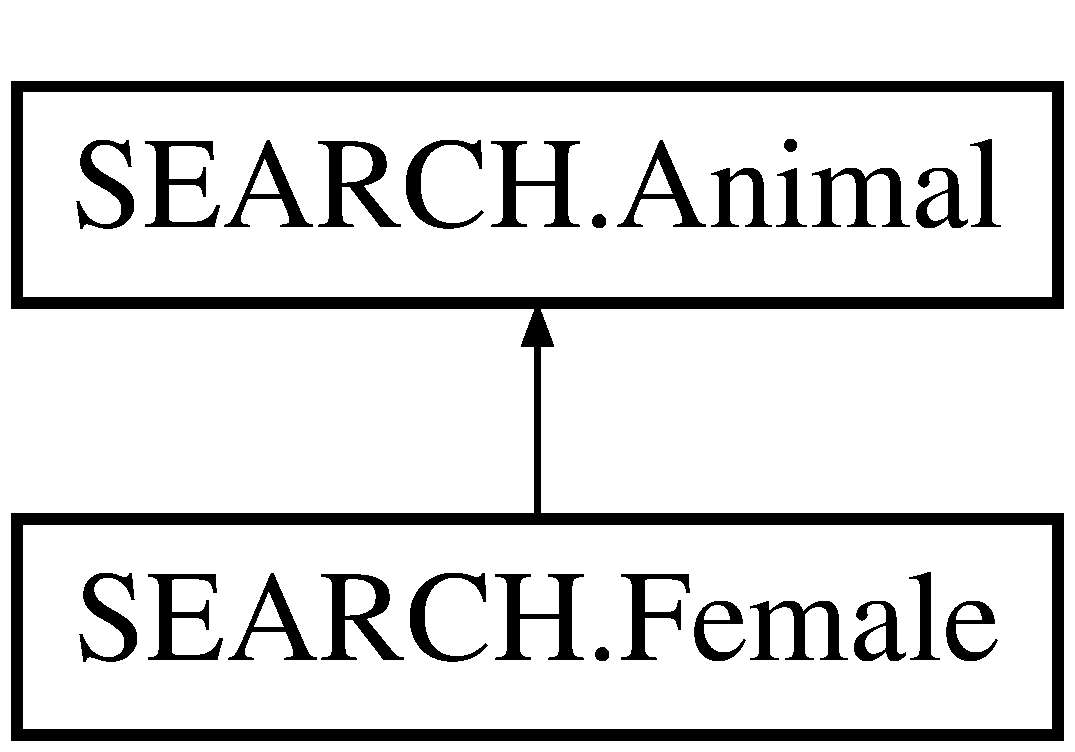
\includegraphics[height=2.000000cm]{class_s_e_a_r_c_h_1_1_female}
\end{center}
\end{figure}
\subsection*{Public Member Functions}
\begin{DoxyCompactItemize}
\item 
\hyperlink{class_s_e_a_r_c_h_1_1_female_a79fd394800ec4c45042483c68494a6d7}{Female} ()
\item 
override void \hyperlink{class_s_e_a_r_c_h_1_1_female_accc345d2bbf2a055b54f67df64a9cdc9}{dump} ()
\end{DoxyCompactItemize}
\subsection*{Additional Inherited Members}


\subsection{Constructor \& Destructor Documentation}
\hypertarget{class_s_e_a_r_c_h_1_1_female_a79fd394800ec4c45042483c68494a6d7}{\index{S\-E\-A\-R\-C\-H\-::\-Female@{S\-E\-A\-R\-C\-H\-::\-Female}!Female@{Female}}
\index{Female@{Female}!SEARCH::Female@{S\-E\-A\-R\-C\-H\-::\-Female}}
\subsubsection[{Female}]{\setlength{\rightskip}{0pt plus 5cm}S\-E\-A\-R\-C\-H.\-Female.\-Female (
\begin{DoxyParamCaption}
{}
\end{DoxyParamCaption}
)}}\label{class_s_e_a_r_c_h_1_1_female_a79fd394800ec4c45042483c68494a6d7}


\subsection{Member Function Documentation}
\hypertarget{class_s_e_a_r_c_h_1_1_female_accc345d2bbf2a055b54f67df64a9cdc9}{\index{S\-E\-A\-R\-C\-H\-::\-Female@{S\-E\-A\-R\-C\-H\-::\-Female}!dump@{dump}}
\index{dump@{dump}!SEARCH::Female@{S\-E\-A\-R\-C\-H\-::\-Female}}
\subsubsection[{dump}]{\setlength{\rightskip}{0pt plus 5cm}override void S\-E\-A\-R\-C\-H.\-Female.\-dump (
\begin{DoxyParamCaption}
{}
\end{DoxyParamCaption}
)\hspace{0.3cm}{\ttfamily [virtual]}}}\label{class_s_e_a_r_c_h_1_1_female_accc345d2bbf2a055b54f67df64a9cdc9}


Reimplemented from \hyperlink{class_s_e_a_r_c_h_1_1_animal_ade2aab75e98f185a6f9ab2a5a9244bd3}{S\-E\-A\-R\-C\-H.\-Animal}.



The documentation for this class was generated from the following file\-:\begin{DoxyCompactItemize}
\item 
Desktop/vlog4net\-A\-R\-C10\-\_\-64\-\_\-newhoming/\-Data\-Centric/\hyperlink{_female_animal_8cs}{Female\-Animal.\-cs}\end{DoxyCompactItemize}

\hypertarget{class_s_e_a_r_c_h_1_1_female_modifier}{\section{S\-E\-A\-R\-C\-H.\-Female\-Modifier Class Reference}
\label{class_s_e_a_r_c_h_1_1_female_modifier}\index{S\-E\-A\-R\-C\-H.\-Female\-Modifier@{S\-E\-A\-R\-C\-H.\-Female\-Modifier}}
}


Modifies the animals behaviors based on the fact it is a female. -\/\-The Singleton defines an Instance operation that lets clients access its unique instance. -\/\-It may be responsible for creating its own unique instance.  


Inheritance diagram for S\-E\-A\-R\-C\-H.\-Female\-Modifier\-:\begin{figure}[H]
\begin{center}
\leavevmode
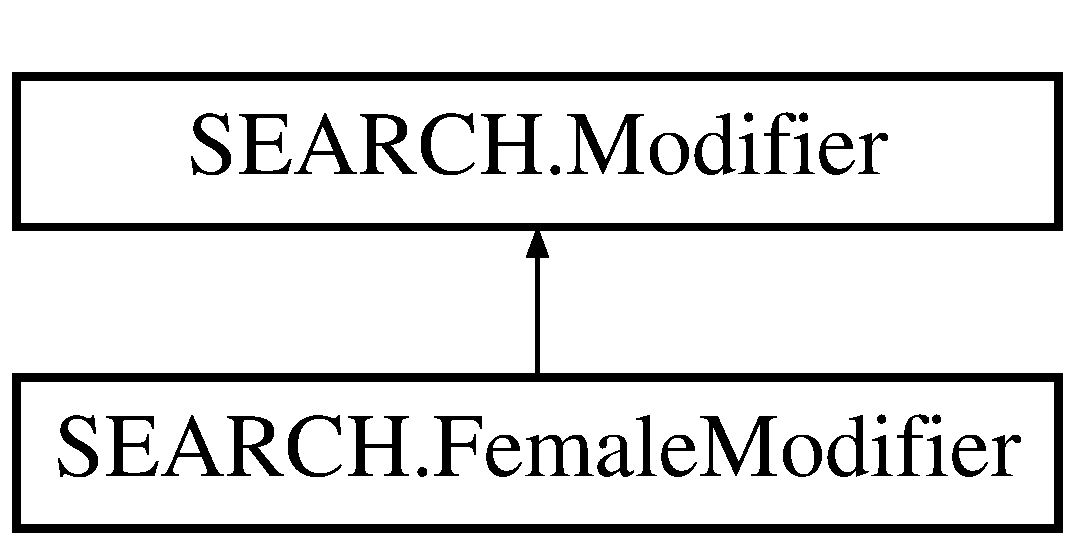
\includegraphics[height=2.000000cm]{class_s_e_a_r_c_h_1_1_female_modifier}
\end{center}
\end{figure}
\subsection*{Static Public Member Functions}
\begin{DoxyCompactItemize}
\item 
static \hyperlink{class_s_e_a_r_c_h_1_1_female_modifier}{Female\-Modifier} \hyperlink{class_s_e_a_r_c_h_1_1_female_modifier_a1fe761214840ce6676c4dacf425c6643}{Get\-Unique\-Instance} ()
\begin{DoxyCompactList}\small\item\em -\/\-This operation implements the logic for returning the unique instance of the Singleton pattern. \end{DoxyCompactList}\end{DoxyCompactItemize}
\subsection*{Additional Inherited Members}


\subsection{Detailed Description}
Modifies the animals behaviors based on the fact it is a female. -\/\-The Singleton defines an Instance operation that lets clients access its unique instance. -\/\-It may be responsible for creating its own unique instance. 



\subsection{Member Function Documentation}
\hypertarget{class_s_e_a_r_c_h_1_1_female_modifier_a1fe761214840ce6676c4dacf425c6643}{\index{S\-E\-A\-R\-C\-H\-::\-Female\-Modifier@{S\-E\-A\-R\-C\-H\-::\-Female\-Modifier}!Get\-Unique\-Instance@{Get\-Unique\-Instance}}
\index{Get\-Unique\-Instance@{Get\-Unique\-Instance}!SEARCH::FemaleModifier@{S\-E\-A\-R\-C\-H\-::\-Female\-Modifier}}
\subsubsection[{Get\-Unique\-Instance}]{\setlength{\rightskip}{0pt plus 5cm}static {\bf Female\-Modifier} S\-E\-A\-R\-C\-H.\-Female\-Modifier.\-Get\-Unique\-Instance (
\begin{DoxyParamCaption}
{}
\end{DoxyParamCaption}
)\hspace{0.3cm}{\ttfamily [static]}}}\label{class_s_e_a_r_c_h_1_1_female_modifier_a1fe761214840ce6676c4dacf425c6643}


-\/\-This operation implements the logic for returning the unique instance of the Singleton pattern. 



The documentation for this class was generated from the following file\-:\begin{DoxyCompactItemize}
\item 
Desktop/vlog4net\-A\-R\-C10\-\_\-64\-\_\-newhoming/\-Data\-Centric/\hyperlink{_female_modifier_8cs}{Female\-Modifier.\-cs}\end{DoxyCompactItemize}

\hypertarget{class_s_e_a_r_c_h_1_1frm_input}{\section{S\-E\-A\-R\-C\-H.\-frm\-Input Class Reference}
\label{class_s_e_a_r_c_h_1_1frm_input}\index{S\-E\-A\-R\-C\-H.\-frm\-Input@{S\-E\-A\-R\-C\-H.\-frm\-Input}}
}


Summary description for Form1.  


Inheritance diagram for S\-E\-A\-R\-C\-H.\-frm\-Input\-:\begin{figure}[H]
\begin{center}
\leavevmode
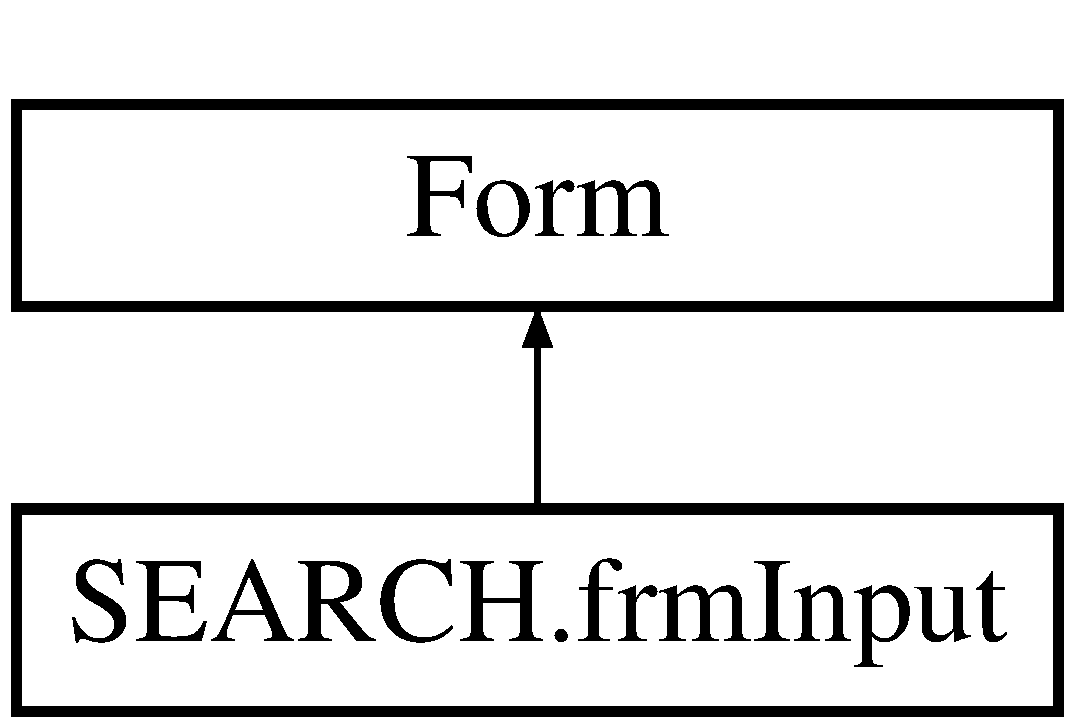
\includegraphics[height=2.000000cm]{class_s_e_a_r_c_h_1_1frm_input}
\end{center}
\end{figure}
\subsection*{Public Member Functions}
\begin{DoxyCompactItemize}
\item 
\hyperlink{class_s_e_a_r_c_h_1_1frm_input_aef8aca701799d18fc50d3996e74e362a}{frm\-Input} ()
\item 
void \hyperlink{class_s_e_a_r_c_h_1_1frm_input_af224be2bfaa8ba98bd554cbf6879b62f}{update\-Progress\-Bar} (double in\-Percent)
\end{DoxyCompactItemize}
\subsection*{Protected Member Functions}
\begin{DoxyCompactItemize}
\item 
override void \hyperlink{class_s_e_a_r_c_h_1_1frm_input_a3749220065441a91720e838a1f8d8e2e}{Dispose} (bool disposing)
\begin{DoxyCompactList}\small\item\em Clean up any resources being used. \end{DoxyCompactList}\end{DoxyCompactItemize}


\subsection{Detailed Description}
Summary description for Form1. 



\subsection{Constructor \& Destructor Documentation}
\hypertarget{class_s_e_a_r_c_h_1_1frm_input_aef8aca701799d18fc50d3996e74e362a}{\index{S\-E\-A\-R\-C\-H\-::frm\-Input@{S\-E\-A\-R\-C\-H\-::frm\-Input}!frm\-Input@{frm\-Input}}
\index{frm\-Input@{frm\-Input}!SEARCH::frmInput@{S\-E\-A\-R\-C\-H\-::frm\-Input}}
\subsubsection[{frm\-Input}]{\setlength{\rightskip}{0pt plus 5cm}S\-E\-A\-R\-C\-H.\-frm\-Input.\-frm\-Input (
\begin{DoxyParamCaption}
{}
\end{DoxyParamCaption}
)}}\label{class_s_e_a_r_c_h_1_1frm_input_aef8aca701799d18fc50d3996e74e362a}


\subsection{Member Function Documentation}
\hypertarget{class_s_e_a_r_c_h_1_1frm_input_a3749220065441a91720e838a1f8d8e2e}{\index{S\-E\-A\-R\-C\-H\-::frm\-Input@{S\-E\-A\-R\-C\-H\-::frm\-Input}!Dispose@{Dispose}}
\index{Dispose@{Dispose}!SEARCH::frmInput@{S\-E\-A\-R\-C\-H\-::frm\-Input}}
\subsubsection[{Dispose}]{\setlength{\rightskip}{0pt plus 5cm}override void S\-E\-A\-R\-C\-H.\-frm\-Input.\-Dispose (
\begin{DoxyParamCaption}
\item[{bool}]{disposing}
\end{DoxyParamCaption}
)\hspace{0.3cm}{\ttfamily [protected]}}}\label{class_s_e_a_r_c_h_1_1frm_input_a3749220065441a91720e838a1f8d8e2e}


Clean up any resources being used. 

\hypertarget{class_s_e_a_r_c_h_1_1frm_input_af224be2bfaa8ba98bd554cbf6879b62f}{\index{S\-E\-A\-R\-C\-H\-::frm\-Input@{S\-E\-A\-R\-C\-H\-::frm\-Input}!update\-Progress\-Bar@{update\-Progress\-Bar}}
\index{update\-Progress\-Bar@{update\-Progress\-Bar}!SEARCH::frmInput@{S\-E\-A\-R\-C\-H\-::frm\-Input}}
\subsubsection[{update\-Progress\-Bar}]{\setlength{\rightskip}{0pt plus 5cm}void S\-E\-A\-R\-C\-H.\-frm\-Input.\-update\-Progress\-Bar (
\begin{DoxyParamCaption}
\item[{double}]{in\-Percent}
\end{DoxyParamCaption}
)}}\label{class_s_e_a_r_c_h_1_1frm_input_af224be2bfaa8ba98bd554cbf6879b62f}


The documentation for this class was generated from the following file\-:\begin{DoxyCompactItemize}
\item 
Desktop/vlog4net\-A\-R\-C10\-\_\-64\-\_\-newhoming/\-Data\-Centric/\hyperlink{frm_input_8cs}{frm\-Input.\-cs}\end{DoxyCompactItemize}

\hypertarget{class_s_e_a_r_c_h_1_1frm_map_select_form}{\section{S\-E\-A\-R\-C\-H.\-frm\-Map\-Select\-Form Class Reference}
\label{class_s_e_a_r_c_h_1_1frm_map_select_form}\index{S\-E\-A\-R\-C\-H.\-frm\-Map\-Select\-Form@{S\-E\-A\-R\-C\-H.\-frm\-Map\-Select\-Form}}
}


Summary description for Map\-Select\-Form.  


Inheritance diagram for S\-E\-A\-R\-C\-H.\-frm\-Map\-Select\-Form\-:\begin{figure}[H]
\begin{center}
\leavevmode
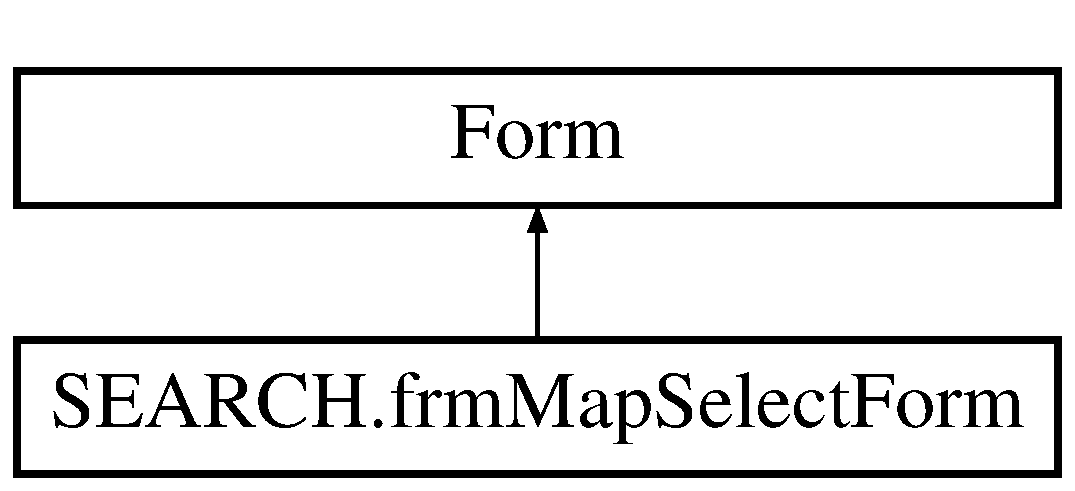
\includegraphics[height=2.000000cm]{class_s_e_a_r_c_h_1_1frm_map_select_form}
\end{center}
\end{figure}
\subsection*{Public Member Functions}
\begin{DoxyCompactItemize}
\item 
\hyperlink{class_s_e_a_r_c_h_1_1frm_map_select_form_a52539ec9e86aa288afbdbb9b3df116af}{frm\-Map\-Select\-Form} ()
\item 
\hyperlink{class_s_e_a_r_c_h_1_1frm_map_select_form_ae06ca96d108e91b4c9c9eed860e26a87}{frm\-Map\-Select\-Form} (string map\-Type, string map\-Path, ref \hyperlink{class_s_e_a_r_c_h_1_1_simulaton_manager}{Simulaton\-Manager} in\-Sim\-Manager)
\item 
\hyperlink{class_s_e_a_r_c_h_1_1frm_map_select_form_a7ff0313a16b3704222aa8c84badcf558}{frm\-Map\-Select\-Form} (ref \hyperlink{class_s_e_a_r_c_h_1_1_simulaton_manager}{Simulaton\-Manager} in\-Sim\-Manager, ref \hyperlink{class_s_e_a_r_c_h_1_1_map_swap_trigger}{Map\-Swap\-Trigger} mst, String m\-Map\-Type, string map\-Path)
\item 
\hyperlink{class_s_e_a_r_c_h_1_1frm_map_select_form_a8710b9cd210fdc9f599ef639d1e58dd0}{frm\-Map\-Select\-Form} (string map\-Type, string map\-Path)
\item 
void \hyperlink{class_s_e_a_r_c_h_1_1frm_map_select_form_a0214c48fd59d029aac1a3bd517d911b4}{fill\-Display} (string year, string day, string hour)
\item 
void \hyperlink{class_s_e_a_r_c_h_1_1frm_map_select_form_a336cd379724bbd241672b0752d21bec2}{set\-Cal\-Range} (Date\-Time start\-Date, Date\-Time end\-Date)
\item 
void \hyperlink{class_s_e_a_r_c_h_1_1frm_map_select_form_a41b0410bd11373d32b718bc44005be5e}{reset\-Cal\-Range} (Date\-Time new\-Start\-Date)
\end{DoxyCompactItemize}
\subsection*{Protected Member Functions}
\begin{DoxyCompactItemize}
\item 
override void \hyperlink{class_s_e_a_r_c_h_1_1frm_map_select_form_a7c0894ccbaf77f3e1a20f6513b22e899}{Dispose} (bool disposing)
\begin{DoxyCompactList}\small\item\em Clean up any resources being used. \end{DoxyCompactList}\end{DoxyCompactItemize}
\subsection*{Properties}
\begin{DoxyCompactItemize}
\item 
\hyperlink{class_s_e_a_r_c_h_1_1_map_swap_trigger}{Map\-Swap\-Trigger} \hyperlink{class_s_e_a_r_c_h_1_1frm_map_select_form_a340701db8706e8a0921814d0d4bccf42}{Mst}\hspace{0.3cm}{\ttfamily  \mbox{[}get, set\mbox{]}}
\item 
bool \hyperlink{class_s_e_a_r_c_h_1_1frm_map_select_form_afa13153f55d301ef1db46eeabc5a4a00}{Cancel}\hspace{0.3cm}{\ttfamily  \mbox{[}get, set\mbox{]}}
\end{DoxyCompactItemize}


\subsection{Detailed Description}
Summary description for Map\-Select\-Form. 



\subsection{Constructor \& Destructor Documentation}
\hypertarget{class_s_e_a_r_c_h_1_1frm_map_select_form_a52539ec9e86aa288afbdbb9b3df116af}{\index{S\-E\-A\-R\-C\-H\-::frm\-Map\-Select\-Form@{S\-E\-A\-R\-C\-H\-::frm\-Map\-Select\-Form}!frm\-Map\-Select\-Form@{frm\-Map\-Select\-Form}}
\index{frm\-Map\-Select\-Form@{frm\-Map\-Select\-Form}!SEARCH::frmMapSelectForm@{S\-E\-A\-R\-C\-H\-::frm\-Map\-Select\-Form}}
\subsubsection[{frm\-Map\-Select\-Form}]{\setlength{\rightskip}{0pt plus 5cm}S\-E\-A\-R\-C\-H.\-frm\-Map\-Select\-Form.\-frm\-Map\-Select\-Form (
\begin{DoxyParamCaption}
{}
\end{DoxyParamCaption}
)}}\label{class_s_e_a_r_c_h_1_1frm_map_select_form_a52539ec9e86aa288afbdbb9b3df116af}
\hypertarget{class_s_e_a_r_c_h_1_1frm_map_select_form_ae06ca96d108e91b4c9c9eed860e26a87}{\index{S\-E\-A\-R\-C\-H\-::frm\-Map\-Select\-Form@{S\-E\-A\-R\-C\-H\-::frm\-Map\-Select\-Form}!frm\-Map\-Select\-Form@{frm\-Map\-Select\-Form}}
\index{frm\-Map\-Select\-Form@{frm\-Map\-Select\-Form}!SEARCH::frmMapSelectForm@{S\-E\-A\-R\-C\-H\-::frm\-Map\-Select\-Form}}
\subsubsection[{frm\-Map\-Select\-Form}]{\setlength{\rightskip}{0pt plus 5cm}S\-E\-A\-R\-C\-H.\-frm\-Map\-Select\-Form.\-frm\-Map\-Select\-Form (
\begin{DoxyParamCaption}
\item[{string}]{map\-Type, }
\item[{string}]{map\-Path, }
\item[{ref {\bf Simulaton\-Manager}}]{in\-Sim\-Manager}
\end{DoxyParamCaption}
)}}\label{class_s_e_a_r_c_h_1_1frm_map_select_form_ae06ca96d108e91b4c9c9eed860e26a87}
\hypertarget{class_s_e_a_r_c_h_1_1frm_map_select_form_a7ff0313a16b3704222aa8c84badcf558}{\index{S\-E\-A\-R\-C\-H\-::frm\-Map\-Select\-Form@{S\-E\-A\-R\-C\-H\-::frm\-Map\-Select\-Form}!frm\-Map\-Select\-Form@{frm\-Map\-Select\-Form}}
\index{frm\-Map\-Select\-Form@{frm\-Map\-Select\-Form}!SEARCH::frmMapSelectForm@{S\-E\-A\-R\-C\-H\-::frm\-Map\-Select\-Form}}
\subsubsection[{frm\-Map\-Select\-Form}]{\setlength{\rightskip}{0pt plus 5cm}S\-E\-A\-R\-C\-H.\-frm\-Map\-Select\-Form.\-frm\-Map\-Select\-Form (
\begin{DoxyParamCaption}
\item[{ref {\bf Simulaton\-Manager}}]{in\-Sim\-Manager, }
\item[{ref {\bf Map\-Swap\-Trigger}}]{mst, }
\item[{String}]{m\-Map\-Type, }
\item[{string}]{map\-Path}
\end{DoxyParamCaption}
)}}\label{class_s_e_a_r_c_h_1_1frm_map_select_form_a7ff0313a16b3704222aa8c84badcf558}
\hypertarget{class_s_e_a_r_c_h_1_1frm_map_select_form_a8710b9cd210fdc9f599ef639d1e58dd0}{\index{S\-E\-A\-R\-C\-H\-::frm\-Map\-Select\-Form@{S\-E\-A\-R\-C\-H\-::frm\-Map\-Select\-Form}!frm\-Map\-Select\-Form@{frm\-Map\-Select\-Form}}
\index{frm\-Map\-Select\-Form@{frm\-Map\-Select\-Form}!SEARCH::frmMapSelectForm@{S\-E\-A\-R\-C\-H\-::frm\-Map\-Select\-Form}}
\subsubsection[{frm\-Map\-Select\-Form}]{\setlength{\rightskip}{0pt plus 5cm}S\-E\-A\-R\-C\-H.\-frm\-Map\-Select\-Form.\-frm\-Map\-Select\-Form (
\begin{DoxyParamCaption}
\item[{string}]{map\-Type, }
\item[{string}]{map\-Path}
\end{DoxyParamCaption}
)}}\label{class_s_e_a_r_c_h_1_1frm_map_select_form_a8710b9cd210fdc9f599ef639d1e58dd0}


\subsection{Member Function Documentation}
\hypertarget{class_s_e_a_r_c_h_1_1frm_map_select_form_a7c0894ccbaf77f3e1a20f6513b22e899}{\index{S\-E\-A\-R\-C\-H\-::frm\-Map\-Select\-Form@{S\-E\-A\-R\-C\-H\-::frm\-Map\-Select\-Form}!Dispose@{Dispose}}
\index{Dispose@{Dispose}!SEARCH::frmMapSelectForm@{S\-E\-A\-R\-C\-H\-::frm\-Map\-Select\-Form}}
\subsubsection[{Dispose}]{\setlength{\rightskip}{0pt plus 5cm}override void S\-E\-A\-R\-C\-H.\-frm\-Map\-Select\-Form.\-Dispose (
\begin{DoxyParamCaption}
\item[{bool}]{disposing}
\end{DoxyParamCaption}
)\hspace{0.3cm}{\ttfamily [protected]}}}\label{class_s_e_a_r_c_h_1_1frm_map_select_form_a7c0894ccbaf77f3e1a20f6513b22e899}


Clean up any resources being used. 

\hypertarget{class_s_e_a_r_c_h_1_1frm_map_select_form_a0214c48fd59d029aac1a3bd517d911b4}{\index{S\-E\-A\-R\-C\-H\-::frm\-Map\-Select\-Form@{S\-E\-A\-R\-C\-H\-::frm\-Map\-Select\-Form}!fill\-Display@{fill\-Display}}
\index{fill\-Display@{fill\-Display}!SEARCH::frmMapSelectForm@{S\-E\-A\-R\-C\-H\-::frm\-Map\-Select\-Form}}
\subsubsection[{fill\-Display}]{\setlength{\rightskip}{0pt plus 5cm}void S\-E\-A\-R\-C\-H.\-frm\-Map\-Select\-Form.\-fill\-Display (
\begin{DoxyParamCaption}
\item[{string}]{year, }
\item[{string}]{day, }
\item[{string}]{hour}
\end{DoxyParamCaption}
)}}\label{class_s_e_a_r_c_h_1_1frm_map_select_form_a0214c48fd59d029aac1a3bd517d911b4}
\hypertarget{class_s_e_a_r_c_h_1_1frm_map_select_form_a41b0410bd11373d32b718bc44005be5e}{\index{S\-E\-A\-R\-C\-H\-::frm\-Map\-Select\-Form@{S\-E\-A\-R\-C\-H\-::frm\-Map\-Select\-Form}!reset\-Cal\-Range@{reset\-Cal\-Range}}
\index{reset\-Cal\-Range@{reset\-Cal\-Range}!SEARCH::frmMapSelectForm@{S\-E\-A\-R\-C\-H\-::frm\-Map\-Select\-Form}}
\subsubsection[{reset\-Cal\-Range}]{\setlength{\rightskip}{0pt plus 5cm}void S\-E\-A\-R\-C\-H.\-frm\-Map\-Select\-Form.\-reset\-Cal\-Range (
\begin{DoxyParamCaption}
\item[{Date\-Time}]{new\-Start\-Date}
\end{DoxyParamCaption}
)}}\label{class_s_e_a_r_c_h_1_1frm_map_select_form_a41b0410bd11373d32b718bc44005be5e}
\hypertarget{class_s_e_a_r_c_h_1_1frm_map_select_form_a336cd379724bbd241672b0752d21bec2}{\index{S\-E\-A\-R\-C\-H\-::frm\-Map\-Select\-Form@{S\-E\-A\-R\-C\-H\-::frm\-Map\-Select\-Form}!set\-Cal\-Range@{set\-Cal\-Range}}
\index{set\-Cal\-Range@{set\-Cal\-Range}!SEARCH::frmMapSelectForm@{S\-E\-A\-R\-C\-H\-::frm\-Map\-Select\-Form}}
\subsubsection[{set\-Cal\-Range}]{\setlength{\rightskip}{0pt plus 5cm}void S\-E\-A\-R\-C\-H.\-frm\-Map\-Select\-Form.\-set\-Cal\-Range (
\begin{DoxyParamCaption}
\item[{Date\-Time}]{start\-Date, }
\item[{Date\-Time}]{end\-Date}
\end{DoxyParamCaption}
)}}\label{class_s_e_a_r_c_h_1_1frm_map_select_form_a336cd379724bbd241672b0752d21bec2}


\subsection{Property Documentation}
\hypertarget{class_s_e_a_r_c_h_1_1frm_map_select_form_afa13153f55d301ef1db46eeabc5a4a00}{\index{S\-E\-A\-R\-C\-H\-::frm\-Map\-Select\-Form@{S\-E\-A\-R\-C\-H\-::frm\-Map\-Select\-Form}!Cancel@{Cancel}}
\index{Cancel@{Cancel}!SEARCH::frmMapSelectForm@{S\-E\-A\-R\-C\-H\-::frm\-Map\-Select\-Form}}
\subsubsection[{Cancel}]{\setlength{\rightskip}{0pt plus 5cm}bool S\-E\-A\-R\-C\-H.\-frm\-Map\-Select\-Form.\-Cancel\hspace{0.3cm}{\ttfamily [get]}, {\ttfamily [set]}}}\label{class_s_e_a_r_c_h_1_1frm_map_select_form_afa13153f55d301ef1db46eeabc5a4a00}
\hypertarget{class_s_e_a_r_c_h_1_1frm_map_select_form_a340701db8706e8a0921814d0d4bccf42}{\index{S\-E\-A\-R\-C\-H\-::frm\-Map\-Select\-Form@{S\-E\-A\-R\-C\-H\-::frm\-Map\-Select\-Form}!Mst@{Mst}}
\index{Mst@{Mst}!SEARCH::frmMapSelectForm@{S\-E\-A\-R\-C\-H\-::frm\-Map\-Select\-Form}}
\subsubsection[{Mst}]{\setlength{\rightskip}{0pt plus 5cm}{\bf Map\-Swap\-Trigger} S\-E\-A\-R\-C\-H.\-frm\-Map\-Select\-Form.\-Mst\hspace{0.3cm}{\ttfamily [get]}, {\ttfamily [set]}}}\label{class_s_e_a_r_c_h_1_1frm_map_select_form_a340701db8706e8a0921814d0d4bccf42}


The documentation for this class was generated from the following file\-:\begin{DoxyCompactItemize}
\item 
Desktop/vlog4net\-A\-R\-C10\-\_\-64\-\_\-newhoming/\-Data\-Centric/\hyperlink{frm_map_select_form_8cs}{frm\-Map\-Select\-Form.\-cs}\end{DoxyCompactItemize}

\hypertarget{class_s_e_a_r_c_h_1_1frm_map_times}{\section{S\-E\-A\-R\-C\-H.\-frm\-Map\-Times Class Reference}
\label{class_s_e_a_r_c_h_1_1frm_map_times}\index{S\-E\-A\-R\-C\-H.\-frm\-Map\-Times@{S\-E\-A\-R\-C\-H.\-frm\-Map\-Times}}
}


Summary description for \hyperlink{class_s_e_a_r_c_h_1_1frm_map_times}{frm\-Map\-Times}.  


Inheritance diagram for S\-E\-A\-R\-C\-H.\-frm\-Map\-Times\-:\begin{figure}[H]
\begin{center}
\leavevmode
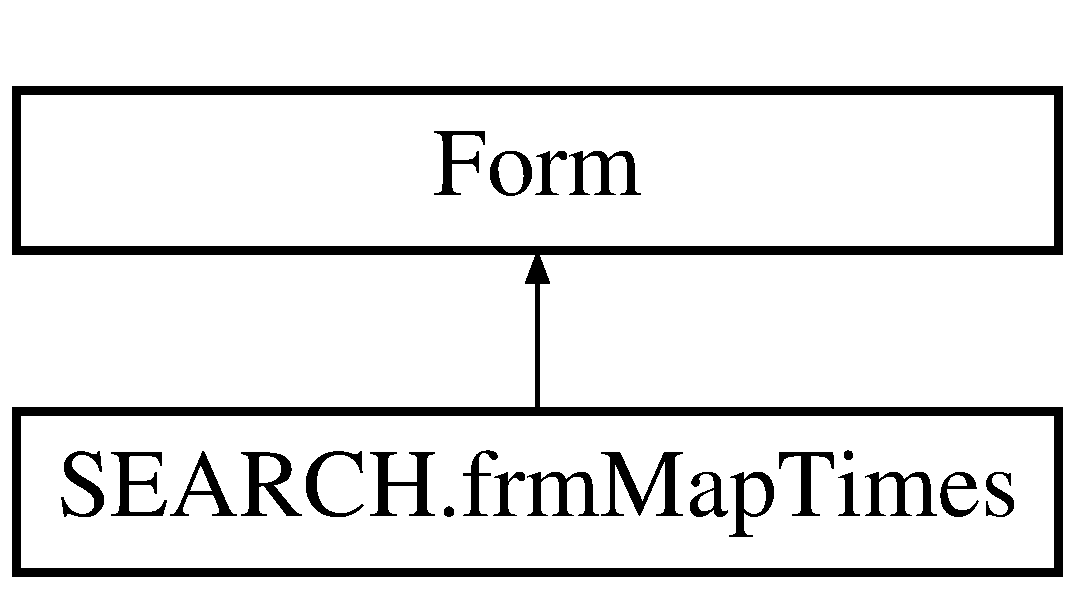
\includegraphics[height=2.000000cm]{class_s_e_a_r_c_h_1_1frm_map_times}
\end{center}
\end{figure}
\subsection*{Public Member Functions}
\begin{DoxyCompactItemize}
\item 
\hyperlink{class_s_e_a_r_c_h_1_1frm_map_times_ae48489a3e6a7d31d7af5abf36a2cc3f1}{frm\-Map\-Times} (ref \hyperlink{class_s_e_a_r_c_h_1_1_simulaton_manager}{Simulaton\-Manager} in\-Sim\-Manager, ref \hyperlink{class_s_e_a_r_c_h_1_1_map_swap_trigger}{Map\-Swap\-Trigger} tmp\-Mst, String m\-Map\-Type)
\item 
\hyperlink{class_s_e_a_r_c_h_1_1frm_map_times_a7c723815a75d7e0838c47e96698dfba5}{frm\-Map\-Times} (ref \hyperlink{class_s_e_a_r_c_h_1_1_simulaton_manager}{Simulaton\-Manager} sm)
\item 
void \hyperlink{class_s_e_a_r_c_h_1_1frm_map_times_ae9b425c5ad54d0010a535e95cba593dc}{set\-Lable} (string text)
\end{DoxyCompactItemize}
\subsection*{Protected Member Functions}
\begin{DoxyCompactItemize}
\item 
override void \hyperlink{class_s_e_a_r_c_h_1_1frm_map_times_aa721e91db1b8b9c446b391ab991a0b50}{Dispose} (bool disposing)
\begin{DoxyCompactList}\small\item\em Clean up any resources being used. \end{DoxyCompactList}\end{DoxyCompactItemize}
\subsection*{Properties}
\begin{DoxyCompactItemize}
\item 
string\mbox{[}$\,$\mbox{]} \hyperlink{class_s_e_a_r_c_h_1_1frm_map_times_ac648bde754f83ee72cee39adb3b9c531}{Out\-File\-Names\-And\-Start\-Times}\hspace{0.3cm}{\ttfamily  \mbox{[}get, set\mbox{]}}
\end{DoxyCompactItemize}


\subsection{Detailed Description}
Summary description for \hyperlink{class_s_e_a_r_c_h_1_1frm_map_times}{frm\-Map\-Times}. 



\subsection{Constructor \& Destructor Documentation}
\hypertarget{class_s_e_a_r_c_h_1_1frm_map_times_ae48489a3e6a7d31d7af5abf36a2cc3f1}{\index{S\-E\-A\-R\-C\-H\-::frm\-Map\-Times@{S\-E\-A\-R\-C\-H\-::frm\-Map\-Times}!frm\-Map\-Times@{frm\-Map\-Times}}
\index{frm\-Map\-Times@{frm\-Map\-Times}!SEARCH::frmMapTimes@{S\-E\-A\-R\-C\-H\-::frm\-Map\-Times}}
\subsubsection[{frm\-Map\-Times}]{\setlength{\rightskip}{0pt plus 5cm}S\-E\-A\-R\-C\-H.\-frm\-Map\-Times.\-frm\-Map\-Times (
\begin{DoxyParamCaption}
\item[{ref {\bf Simulaton\-Manager}}]{in\-Sim\-Manager, }
\item[{ref {\bf Map\-Swap\-Trigger}}]{tmp\-Mst, }
\item[{String}]{m\-Map\-Type}
\end{DoxyParamCaption}
)}}\label{class_s_e_a_r_c_h_1_1frm_map_times_ae48489a3e6a7d31d7af5abf36a2cc3f1}
\hypertarget{class_s_e_a_r_c_h_1_1frm_map_times_a7c723815a75d7e0838c47e96698dfba5}{\index{S\-E\-A\-R\-C\-H\-::frm\-Map\-Times@{S\-E\-A\-R\-C\-H\-::frm\-Map\-Times}!frm\-Map\-Times@{frm\-Map\-Times}}
\index{frm\-Map\-Times@{frm\-Map\-Times}!SEARCH::frmMapTimes@{S\-E\-A\-R\-C\-H\-::frm\-Map\-Times}}
\subsubsection[{frm\-Map\-Times}]{\setlength{\rightskip}{0pt plus 5cm}S\-E\-A\-R\-C\-H.\-frm\-Map\-Times.\-frm\-Map\-Times (
\begin{DoxyParamCaption}
\item[{ref {\bf Simulaton\-Manager}}]{sm}
\end{DoxyParamCaption}
)}}\label{class_s_e_a_r_c_h_1_1frm_map_times_a7c723815a75d7e0838c47e96698dfba5}


\subsection{Member Function Documentation}
\hypertarget{class_s_e_a_r_c_h_1_1frm_map_times_aa721e91db1b8b9c446b391ab991a0b50}{\index{S\-E\-A\-R\-C\-H\-::frm\-Map\-Times@{S\-E\-A\-R\-C\-H\-::frm\-Map\-Times}!Dispose@{Dispose}}
\index{Dispose@{Dispose}!SEARCH::frmMapTimes@{S\-E\-A\-R\-C\-H\-::frm\-Map\-Times}}
\subsubsection[{Dispose}]{\setlength{\rightskip}{0pt plus 5cm}override void S\-E\-A\-R\-C\-H.\-frm\-Map\-Times.\-Dispose (
\begin{DoxyParamCaption}
\item[{bool}]{disposing}
\end{DoxyParamCaption}
)\hspace{0.3cm}{\ttfamily [protected]}}}\label{class_s_e_a_r_c_h_1_1frm_map_times_aa721e91db1b8b9c446b391ab991a0b50}


Clean up any resources being used. 

\hypertarget{class_s_e_a_r_c_h_1_1frm_map_times_ae9b425c5ad54d0010a535e95cba593dc}{\index{S\-E\-A\-R\-C\-H\-::frm\-Map\-Times@{S\-E\-A\-R\-C\-H\-::frm\-Map\-Times}!set\-Lable@{set\-Lable}}
\index{set\-Lable@{set\-Lable}!SEARCH::frmMapTimes@{S\-E\-A\-R\-C\-H\-::frm\-Map\-Times}}
\subsubsection[{set\-Lable}]{\setlength{\rightskip}{0pt plus 5cm}void S\-E\-A\-R\-C\-H.\-frm\-Map\-Times.\-set\-Lable (
\begin{DoxyParamCaption}
\item[{string}]{text}
\end{DoxyParamCaption}
)}}\label{class_s_e_a_r_c_h_1_1frm_map_times_ae9b425c5ad54d0010a535e95cba593dc}


\subsection{Property Documentation}
\hypertarget{class_s_e_a_r_c_h_1_1frm_map_times_ac648bde754f83ee72cee39adb3b9c531}{\index{S\-E\-A\-R\-C\-H\-::frm\-Map\-Times@{S\-E\-A\-R\-C\-H\-::frm\-Map\-Times}!Out\-File\-Names\-And\-Start\-Times@{Out\-File\-Names\-And\-Start\-Times}}
\index{Out\-File\-Names\-And\-Start\-Times@{Out\-File\-Names\-And\-Start\-Times}!SEARCH::frmMapTimes@{S\-E\-A\-R\-C\-H\-::frm\-Map\-Times}}
\subsubsection[{Out\-File\-Names\-And\-Start\-Times}]{\setlength{\rightskip}{0pt plus 5cm}string \mbox{[}$\,$\mbox{]} S\-E\-A\-R\-C\-H.\-frm\-Map\-Times.\-Out\-File\-Names\-And\-Start\-Times\hspace{0.3cm}{\ttfamily [get]}, {\ttfamily [set]}}}\label{class_s_e_a_r_c_h_1_1frm_map_times_ac648bde754f83ee72cee39adb3b9c531}


The documentation for this class was generated from the following file\-:\begin{DoxyCompactItemize}
\item 
Desktop/vlog4net\-A\-R\-C10\-\_\-64\-\_\-newhoming/\-Data\-Centric/\hyperlink{frm_map_times_8cs}{frm\-Map\-Times.\-cs}\end{DoxyCompactItemize}

\hypertarget{class_s_e_a_r_c_h_1_1frm_modifier_input}{\section{S\-E\-A\-R\-C\-H.\-frm\-Modifier\-Input Class Reference}
\label{class_s_e_a_r_c_h_1_1frm_modifier_input}\index{S\-E\-A\-R\-C\-H.\-frm\-Modifier\-Input@{S\-E\-A\-R\-C\-H.\-frm\-Modifier\-Input}}
}


Summary description for \hyperlink{class_s_e_a_r_c_h_1_1frm_modifier_input}{frm\-Modifier\-Input}.  


Inheritance diagram for S\-E\-A\-R\-C\-H.\-frm\-Modifier\-Input\-:\begin{figure}[H]
\begin{center}
\leavevmode
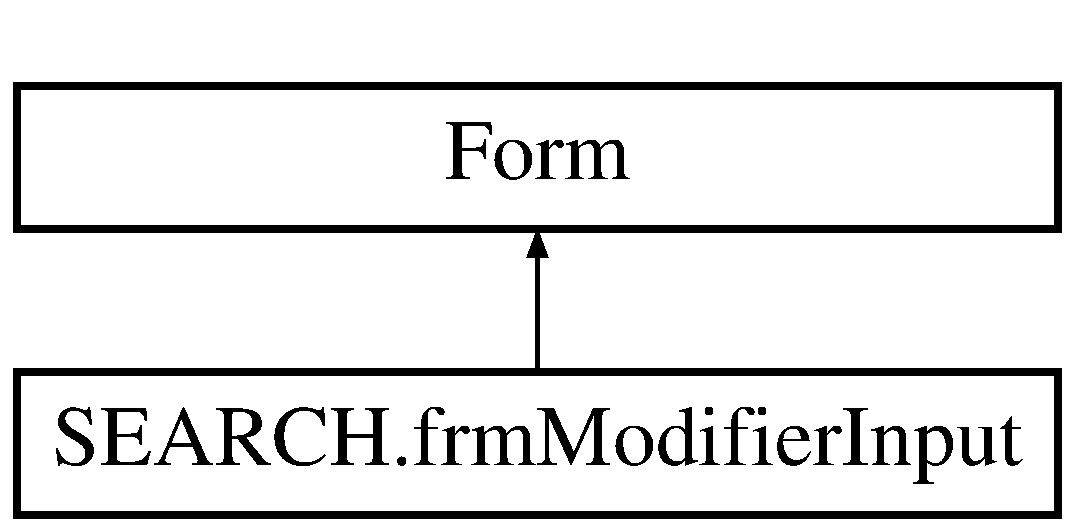
\includegraphics[height=2.000000cm]{class_s_e_a_r_c_h_1_1frm_modifier_input}
\end{center}
\end{figure}
\subsection*{Public Member Functions}
\begin{DoxyCompactItemize}
\item 
\hyperlink{class_s_e_a_r_c_h_1_1frm_modifier_input_a40ce365148ac1f28f502f5ac00e3af45}{frm\-Modifier\-Input} ()
\item 
void \hyperlink{class_s_e_a_r_c_h_1_1frm_modifier_input_a17ab749d0bb216161dc7b5097c3dabb8}{set\-Gender} (string gender\-Type)
\item 
void \hyperlink{class_s_e_a_r_c_h_1_1frm_modifier_input_a15cd673e516352b34d523ef1b9ed61c0}{set\-Hour} ()
\item 
void \hyperlink{class_s_e_a_r_c_h_1_1frm_modifier_input_a1c1d60dfda5e8ff391911592de5a2b40}{set\-Text} (string in\-Text)
\end{DoxyCompactItemize}
\subsection*{Protected Member Functions}
\begin{DoxyCompactItemize}
\item 
override void \hyperlink{class_s_e_a_r_c_h_1_1frm_modifier_input_a04b003e7055df59a2f00cdcdb82ba976}{Dispose} (bool disposing)
\begin{DoxyCompactList}\small\item\em Clean up any resources being used. \end{DoxyCompactList}\end{DoxyCompactItemize}
\subsection*{Properties}
\begin{DoxyCompactItemize}
\item 
Date\-Time \hyperlink{class_s_e_a_r_c_h_1_1frm_modifier_input_aae4ea1b800112742944b3338fedccfd1}{Date}\hspace{0.3cm}{\ttfamily  \mbox{[}get, set\mbox{]}}
\item 
int \hyperlink{class_s_e_a_r_c_h_1_1frm_modifier_input_a1696be177f3cecbecf28f7e2743267d6}{Hour}\hspace{0.3cm}{\ttfamily  \mbox{[}get, set\mbox{]}}
\item 
\hyperlink{class_s_e_a_r_c_h_1_1_modifier}{Modifier} \hyperlink{class_s_e_a_r_c_h_1_1frm_modifier_input_a9d8f7d817e0833d328014551f737632f}{Temp\-Mod}\hspace{0.3cm}{\ttfamily  \mbox{[}get, set\mbox{]}}
\item 
bool \hyperlink{class_s_e_a_r_c_h_1_1frm_modifier_input_ad264b10459496052416016d7ef96639f}{Value}\hspace{0.3cm}{\ttfamily  \mbox{[}get, set\mbox{]}}
\end{DoxyCompactItemize}


\subsection{Detailed Description}
Summary description for \hyperlink{class_s_e_a_r_c_h_1_1frm_modifier_input}{frm\-Modifier\-Input}. 



\subsection{Constructor \& Destructor Documentation}
\hypertarget{class_s_e_a_r_c_h_1_1frm_modifier_input_a40ce365148ac1f28f502f5ac00e3af45}{\index{S\-E\-A\-R\-C\-H\-::frm\-Modifier\-Input@{S\-E\-A\-R\-C\-H\-::frm\-Modifier\-Input}!frm\-Modifier\-Input@{frm\-Modifier\-Input}}
\index{frm\-Modifier\-Input@{frm\-Modifier\-Input}!SEARCH::frmModifierInput@{S\-E\-A\-R\-C\-H\-::frm\-Modifier\-Input}}
\subsubsection[{frm\-Modifier\-Input}]{\setlength{\rightskip}{0pt plus 5cm}S\-E\-A\-R\-C\-H.\-frm\-Modifier\-Input.\-frm\-Modifier\-Input (
\begin{DoxyParamCaption}
{}
\end{DoxyParamCaption}
)}}\label{class_s_e_a_r_c_h_1_1frm_modifier_input_a40ce365148ac1f28f502f5ac00e3af45}


\subsection{Member Function Documentation}
\hypertarget{class_s_e_a_r_c_h_1_1frm_modifier_input_a04b003e7055df59a2f00cdcdb82ba976}{\index{S\-E\-A\-R\-C\-H\-::frm\-Modifier\-Input@{S\-E\-A\-R\-C\-H\-::frm\-Modifier\-Input}!Dispose@{Dispose}}
\index{Dispose@{Dispose}!SEARCH::frmModifierInput@{S\-E\-A\-R\-C\-H\-::frm\-Modifier\-Input}}
\subsubsection[{Dispose}]{\setlength{\rightskip}{0pt plus 5cm}override void S\-E\-A\-R\-C\-H.\-frm\-Modifier\-Input.\-Dispose (
\begin{DoxyParamCaption}
\item[{bool}]{disposing}
\end{DoxyParamCaption}
)\hspace{0.3cm}{\ttfamily [protected]}}}\label{class_s_e_a_r_c_h_1_1frm_modifier_input_a04b003e7055df59a2f00cdcdb82ba976}


Clean up any resources being used. 

\hypertarget{class_s_e_a_r_c_h_1_1frm_modifier_input_a17ab749d0bb216161dc7b5097c3dabb8}{\index{S\-E\-A\-R\-C\-H\-::frm\-Modifier\-Input@{S\-E\-A\-R\-C\-H\-::frm\-Modifier\-Input}!set\-Gender@{set\-Gender}}
\index{set\-Gender@{set\-Gender}!SEARCH::frmModifierInput@{S\-E\-A\-R\-C\-H\-::frm\-Modifier\-Input}}
\subsubsection[{set\-Gender}]{\setlength{\rightskip}{0pt plus 5cm}void S\-E\-A\-R\-C\-H.\-frm\-Modifier\-Input.\-set\-Gender (
\begin{DoxyParamCaption}
\item[{string}]{gender\-Type}
\end{DoxyParamCaption}
)}}\label{class_s_e_a_r_c_h_1_1frm_modifier_input_a17ab749d0bb216161dc7b5097c3dabb8}
\hypertarget{class_s_e_a_r_c_h_1_1frm_modifier_input_a15cd673e516352b34d523ef1b9ed61c0}{\index{S\-E\-A\-R\-C\-H\-::frm\-Modifier\-Input@{S\-E\-A\-R\-C\-H\-::frm\-Modifier\-Input}!set\-Hour@{set\-Hour}}
\index{set\-Hour@{set\-Hour}!SEARCH::frmModifierInput@{S\-E\-A\-R\-C\-H\-::frm\-Modifier\-Input}}
\subsubsection[{set\-Hour}]{\setlength{\rightskip}{0pt plus 5cm}void S\-E\-A\-R\-C\-H.\-frm\-Modifier\-Input.\-set\-Hour (
\begin{DoxyParamCaption}
{}
\end{DoxyParamCaption}
)}}\label{class_s_e_a_r_c_h_1_1frm_modifier_input_a15cd673e516352b34d523ef1b9ed61c0}
\hypertarget{class_s_e_a_r_c_h_1_1frm_modifier_input_a1c1d60dfda5e8ff391911592de5a2b40}{\index{S\-E\-A\-R\-C\-H\-::frm\-Modifier\-Input@{S\-E\-A\-R\-C\-H\-::frm\-Modifier\-Input}!set\-Text@{set\-Text}}
\index{set\-Text@{set\-Text}!SEARCH::frmModifierInput@{S\-E\-A\-R\-C\-H\-::frm\-Modifier\-Input}}
\subsubsection[{set\-Text}]{\setlength{\rightskip}{0pt plus 5cm}void S\-E\-A\-R\-C\-H.\-frm\-Modifier\-Input.\-set\-Text (
\begin{DoxyParamCaption}
\item[{string}]{in\-Text}
\end{DoxyParamCaption}
)}}\label{class_s_e_a_r_c_h_1_1frm_modifier_input_a1c1d60dfda5e8ff391911592de5a2b40}


\subsection{Property Documentation}
\hypertarget{class_s_e_a_r_c_h_1_1frm_modifier_input_aae4ea1b800112742944b3338fedccfd1}{\index{S\-E\-A\-R\-C\-H\-::frm\-Modifier\-Input@{S\-E\-A\-R\-C\-H\-::frm\-Modifier\-Input}!Date@{Date}}
\index{Date@{Date}!SEARCH::frmModifierInput@{S\-E\-A\-R\-C\-H\-::frm\-Modifier\-Input}}
\subsubsection[{Date}]{\setlength{\rightskip}{0pt plus 5cm}Date\-Time S\-E\-A\-R\-C\-H.\-frm\-Modifier\-Input.\-Date\hspace{0.3cm}{\ttfamily [get]}, {\ttfamily [set]}}}\label{class_s_e_a_r_c_h_1_1frm_modifier_input_aae4ea1b800112742944b3338fedccfd1}
\hypertarget{class_s_e_a_r_c_h_1_1frm_modifier_input_a1696be177f3cecbecf28f7e2743267d6}{\index{S\-E\-A\-R\-C\-H\-::frm\-Modifier\-Input@{S\-E\-A\-R\-C\-H\-::frm\-Modifier\-Input}!Hour@{Hour}}
\index{Hour@{Hour}!SEARCH::frmModifierInput@{S\-E\-A\-R\-C\-H\-::frm\-Modifier\-Input}}
\subsubsection[{Hour}]{\setlength{\rightskip}{0pt plus 5cm}int S\-E\-A\-R\-C\-H.\-frm\-Modifier\-Input.\-Hour\hspace{0.3cm}{\ttfamily [get]}, {\ttfamily [set]}}}\label{class_s_e_a_r_c_h_1_1frm_modifier_input_a1696be177f3cecbecf28f7e2743267d6}
\hypertarget{class_s_e_a_r_c_h_1_1frm_modifier_input_a9d8f7d817e0833d328014551f737632f}{\index{S\-E\-A\-R\-C\-H\-::frm\-Modifier\-Input@{S\-E\-A\-R\-C\-H\-::frm\-Modifier\-Input}!Temp\-Mod@{Temp\-Mod}}
\index{Temp\-Mod@{Temp\-Mod}!SEARCH::frmModifierInput@{S\-E\-A\-R\-C\-H\-::frm\-Modifier\-Input}}
\subsubsection[{Temp\-Mod}]{\setlength{\rightskip}{0pt plus 5cm}{\bf Modifier} S\-E\-A\-R\-C\-H.\-frm\-Modifier\-Input.\-Temp\-Mod\hspace{0.3cm}{\ttfamily [get]}, {\ttfamily [set]}}}\label{class_s_e_a_r_c_h_1_1frm_modifier_input_a9d8f7d817e0833d328014551f737632f}
\hypertarget{class_s_e_a_r_c_h_1_1frm_modifier_input_ad264b10459496052416016d7ef96639f}{\index{S\-E\-A\-R\-C\-H\-::frm\-Modifier\-Input@{S\-E\-A\-R\-C\-H\-::frm\-Modifier\-Input}!Value@{Value}}
\index{Value@{Value}!SEARCH::frmModifierInput@{S\-E\-A\-R\-C\-H\-::frm\-Modifier\-Input}}
\subsubsection[{Value}]{\setlength{\rightskip}{0pt plus 5cm}bool S\-E\-A\-R\-C\-H.\-frm\-Modifier\-Input.\-Value\hspace{0.3cm}{\ttfamily [get]}, {\ttfamily [set]}}}\label{class_s_e_a_r_c_h_1_1frm_modifier_input_ad264b10459496052416016d7ef96639f}


The documentation for this class was generated from the following file\-:\begin{DoxyCompactItemize}
\item 
Desktop/vlog4net\-A\-R\-C10\-\_\-64\-\_\-newhoming/\-Data\-Centric/\hyperlink{frm_modifier_input_8cs}{frm\-Modifier\-Input.\-cs}\end{DoxyCompactItemize}

\hypertarget{class_s_e_a_r_c_h_1_1_forms_1_1frm_season}{\section{S\-E\-A\-R\-C\-H.\-Forms.\-frm\-Season Class Reference}
\label{class_s_e_a_r_c_h_1_1_forms_1_1frm_season}\index{S\-E\-A\-R\-C\-H.\-Forms.\-frm\-Season@{S\-E\-A\-R\-C\-H.\-Forms.\-frm\-Season}}
}


Summary description for \hyperlink{class_s_e_a_r_c_h_1_1_forms_1_1frm_season}{frm\-Season}.  


Inheritance diagram for S\-E\-A\-R\-C\-H.\-Forms.\-frm\-Season\-:\begin{figure}[H]
\begin{center}
\leavevmode
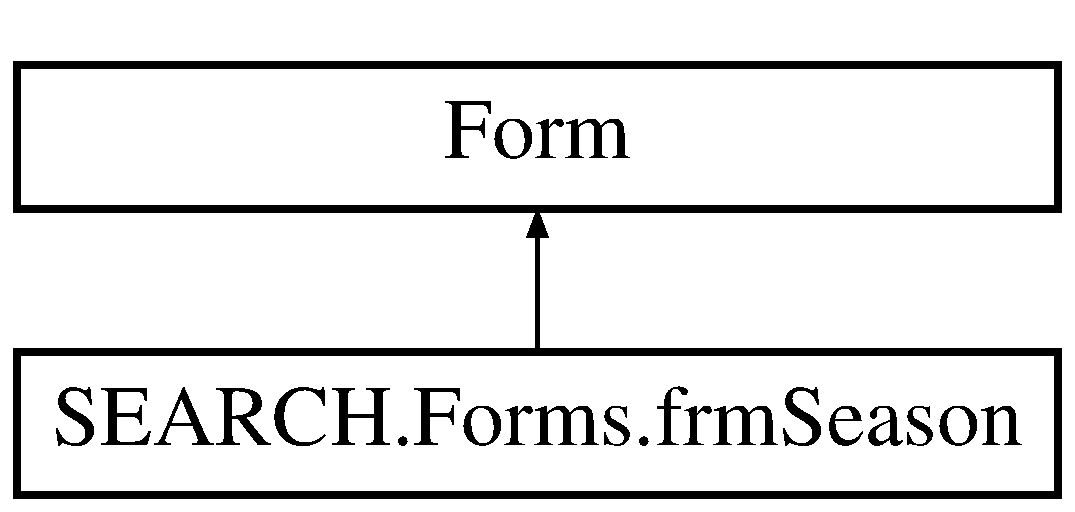
\includegraphics[height=2.000000cm]{class_s_e_a_r_c_h_1_1_forms_1_1frm_season}
\end{center}
\end{figure}
\subsection*{Public Member Functions}
\begin{DoxyCompactItemize}
\item 
\hyperlink{class_s_e_a_r_c_h_1_1_forms_1_1frm_season_ab262d60ce72628aeea6bc49a68acd377}{frm\-Season} (int year, int season, ref Array\-List al, ref \hyperlink{class_s_e_a_r_c_h_1_1_simulaton_manager}{Simulaton\-Manager} sm, string swap\-Year)
\item 
\hyperlink{class_s_e_a_r_c_h_1_1_forms_1_1frm_season_a1a93bdfbcecab718a95ef672be83de10}{frm\-Season} ()
\end{DoxyCompactItemize}
\subsection*{Protected Member Functions}
\begin{DoxyCompactItemize}
\item 
override void \hyperlink{class_s_e_a_r_c_h_1_1_forms_1_1frm_season_a0e765ebfef1574248f7f3099e986c850}{Dispose} (bool disposing)
\begin{DoxyCompactList}\small\item\em Clean up any resources being used. \end{DoxyCompactList}\end{DoxyCompactItemize}


\subsection{Detailed Description}
Summary description for \hyperlink{class_s_e_a_r_c_h_1_1_forms_1_1frm_season}{frm\-Season}. 



\subsection{Constructor \& Destructor Documentation}
\hypertarget{class_s_e_a_r_c_h_1_1_forms_1_1frm_season_ab262d60ce72628aeea6bc49a68acd377}{\index{S\-E\-A\-R\-C\-H\-::\-Forms\-::frm\-Season@{S\-E\-A\-R\-C\-H\-::\-Forms\-::frm\-Season}!frm\-Season@{frm\-Season}}
\index{frm\-Season@{frm\-Season}!SEARCH::Forms::frmSeason@{S\-E\-A\-R\-C\-H\-::\-Forms\-::frm\-Season}}
\subsubsection[{frm\-Season}]{\setlength{\rightskip}{0pt plus 5cm}S\-E\-A\-R\-C\-H.\-Forms.\-frm\-Season.\-frm\-Season (
\begin{DoxyParamCaption}
\item[{int}]{year, }
\item[{int}]{season, }
\item[{ref Array\-List}]{al, }
\item[{ref {\bf Simulaton\-Manager}}]{sm, }
\item[{string}]{swap\-Year}
\end{DoxyParamCaption}
)}}\label{class_s_e_a_r_c_h_1_1_forms_1_1frm_season_ab262d60ce72628aeea6bc49a68acd377}
\hypertarget{class_s_e_a_r_c_h_1_1_forms_1_1frm_season_a1a93bdfbcecab718a95ef672be83de10}{\index{S\-E\-A\-R\-C\-H\-::\-Forms\-::frm\-Season@{S\-E\-A\-R\-C\-H\-::\-Forms\-::frm\-Season}!frm\-Season@{frm\-Season}}
\index{frm\-Season@{frm\-Season}!SEARCH::Forms::frmSeason@{S\-E\-A\-R\-C\-H\-::\-Forms\-::frm\-Season}}
\subsubsection[{frm\-Season}]{\setlength{\rightskip}{0pt plus 5cm}S\-E\-A\-R\-C\-H.\-Forms.\-frm\-Season.\-frm\-Season (
\begin{DoxyParamCaption}
{}
\end{DoxyParamCaption}
)}}\label{class_s_e_a_r_c_h_1_1_forms_1_1frm_season_a1a93bdfbcecab718a95ef672be83de10}


\subsection{Member Function Documentation}
\hypertarget{class_s_e_a_r_c_h_1_1_forms_1_1frm_season_a0e765ebfef1574248f7f3099e986c850}{\index{S\-E\-A\-R\-C\-H\-::\-Forms\-::frm\-Season@{S\-E\-A\-R\-C\-H\-::\-Forms\-::frm\-Season}!Dispose@{Dispose}}
\index{Dispose@{Dispose}!SEARCH::Forms::frmSeason@{S\-E\-A\-R\-C\-H\-::\-Forms\-::frm\-Season}}
\subsubsection[{Dispose}]{\setlength{\rightskip}{0pt plus 5cm}override void S\-E\-A\-R\-C\-H.\-Forms.\-frm\-Season.\-Dispose (
\begin{DoxyParamCaption}
\item[{bool}]{disposing}
\end{DoxyParamCaption}
)\hspace{0.3cm}{\ttfamily [protected]}}}\label{class_s_e_a_r_c_h_1_1_forms_1_1frm_season_a0e765ebfef1574248f7f3099e986c850}


Clean up any resources being used. 



The documentation for this class was generated from the following file\-:\begin{DoxyCompactItemize}
\item 
Desktop/vlog4net\-A\-R\-C10\-\_\-64\-\_\-newhoming/\-Data\-Centric/\hyperlink{frm_season_8cs}{frm\-Season.\-cs}\end{DoxyCompactItemize}

\hypertarget{class_s_e_a_r_c_h_1_1_gender_modifiers}{\section{S\-E\-A\-R\-C\-H.\-Gender\-Modifiers Class Reference}
\label{class_s_e_a_r_c_h_1_1_gender_modifiers}\index{S\-E\-A\-R\-C\-H.\-Gender\-Modifiers@{S\-E\-A\-R\-C\-H.\-Gender\-Modifiers}}
}
Inheritance diagram for S\-E\-A\-R\-C\-H.\-Gender\-Modifiers\-:\begin{figure}[H]
\begin{center}
\leavevmode
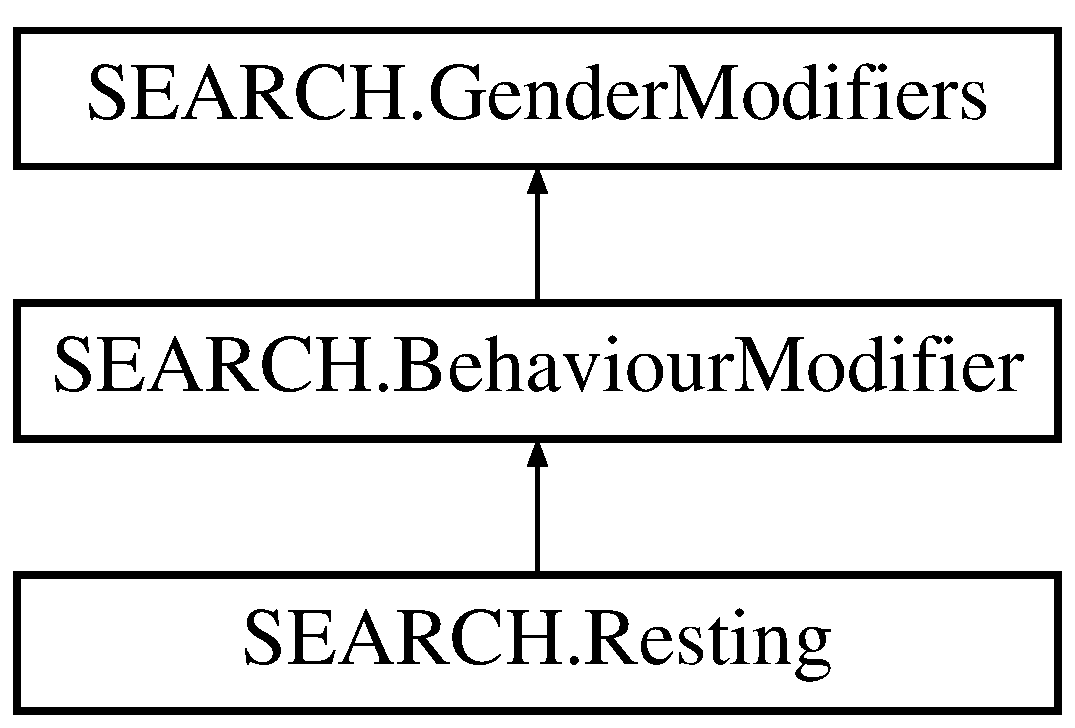
\includegraphics[height=3.000000cm]{class_s_e_a_r_c_h_1_1_gender_modifiers}
\end{center}
\end{figure}
\subsection*{Properties}
\begin{DoxyCompactItemize}
\item 
double \hyperlink{class_s_e_a_r_c_h_1_1_gender_modifiers_a3428fc5be65c38c82cace4ac6ada0587}{Energy\-Used\-Per\-Time\-Step}\hspace{0.3cm}{\ttfamily  \mbox{[}get, set\mbox{]}}
\item 
double \hyperlink{class_s_e_a_r_c_h_1_1_gender_modifiers_adcae5f50fbd812660e119a93d1ae3302}{Move\-Speed}\hspace{0.3cm}{\ttfamily  \mbox{[}get, set\mbox{]}}
\item 
double \hyperlink{class_s_e_a_r_c_h_1_1_gender_modifiers_ab69d24d382bb36907d2f97fb2e4ce107}{Move\-Tortusoity}\hspace{0.3cm}{\ttfamily  \mbox{[}get, set\mbox{]}}
\item 
double \hyperlink{class_s_e_a_r_c_h_1_1_gender_modifiers_a06d62545bc956483f667edc8352d6884}{Prob\-Capture\-Food}\hspace{0.3cm}{\ttfamily  \mbox{[}get, set\mbox{]}}
\item 
double \hyperlink{class_s_e_a_r_c_h_1_1_gender_modifiers_ad3932ec592e9eaeac8266375122ff312}{Prog\-Killed\-By\-Predator}\hspace{0.3cm}{\ttfamily  \mbox{[}get, set\mbox{]}}
\item 
double \hyperlink{class_s_e_a_r_c_h_1_1_gender_modifiers_aef2492f6721cb65c462a84d981331ec5}{Vision\-Range}\hspace{0.3cm}{\ttfamily  \mbox{[}get, set\mbox{]}}
\end{DoxyCompactItemize}


\subsection{Property Documentation}
\hypertarget{class_s_e_a_r_c_h_1_1_gender_modifiers_a3428fc5be65c38c82cace4ac6ada0587}{\index{S\-E\-A\-R\-C\-H\-::\-Gender\-Modifiers@{S\-E\-A\-R\-C\-H\-::\-Gender\-Modifiers}!Energy\-Used\-Per\-Time\-Step@{Energy\-Used\-Per\-Time\-Step}}
\index{Energy\-Used\-Per\-Time\-Step@{Energy\-Used\-Per\-Time\-Step}!SEARCH::GenderModifiers@{S\-E\-A\-R\-C\-H\-::\-Gender\-Modifiers}}
\subsubsection[{Energy\-Used\-Per\-Time\-Step}]{\setlength{\rightskip}{0pt plus 5cm}double S\-E\-A\-R\-C\-H.\-Gender\-Modifiers.\-Energy\-Used\-Per\-Time\-Step\hspace{0.3cm}{\ttfamily [get]}, {\ttfamily [set]}}}\label{class_s_e_a_r_c_h_1_1_gender_modifiers_a3428fc5be65c38c82cace4ac6ada0587}
\hypertarget{class_s_e_a_r_c_h_1_1_gender_modifiers_adcae5f50fbd812660e119a93d1ae3302}{\index{S\-E\-A\-R\-C\-H\-::\-Gender\-Modifiers@{S\-E\-A\-R\-C\-H\-::\-Gender\-Modifiers}!Move\-Speed@{Move\-Speed}}
\index{Move\-Speed@{Move\-Speed}!SEARCH::GenderModifiers@{S\-E\-A\-R\-C\-H\-::\-Gender\-Modifiers}}
\subsubsection[{Move\-Speed}]{\setlength{\rightskip}{0pt plus 5cm}double S\-E\-A\-R\-C\-H.\-Gender\-Modifiers.\-Move\-Speed\hspace{0.3cm}{\ttfamily [get]}, {\ttfamily [set]}}}\label{class_s_e_a_r_c_h_1_1_gender_modifiers_adcae5f50fbd812660e119a93d1ae3302}
\hypertarget{class_s_e_a_r_c_h_1_1_gender_modifiers_ab69d24d382bb36907d2f97fb2e4ce107}{\index{S\-E\-A\-R\-C\-H\-::\-Gender\-Modifiers@{S\-E\-A\-R\-C\-H\-::\-Gender\-Modifiers}!Move\-Tortusoity@{Move\-Tortusoity}}
\index{Move\-Tortusoity@{Move\-Tortusoity}!SEARCH::GenderModifiers@{S\-E\-A\-R\-C\-H\-::\-Gender\-Modifiers}}
\subsubsection[{Move\-Tortusoity}]{\setlength{\rightskip}{0pt plus 5cm}double S\-E\-A\-R\-C\-H.\-Gender\-Modifiers.\-Move\-Tortusoity\hspace{0.3cm}{\ttfamily [get]}, {\ttfamily [set]}}}\label{class_s_e_a_r_c_h_1_1_gender_modifiers_ab69d24d382bb36907d2f97fb2e4ce107}
\hypertarget{class_s_e_a_r_c_h_1_1_gender_modifiers_a06d62545bc956483f667edc8352d6884}{\index{S\-E\-A\-R\-C\-H\-::\-Gender\-Modifiers@{S\-E\-A\-R\-C\-H\-::\-Gender\-Modifiers}!Prob\-Capture\-Food@{Prob\-Capture\-Food}}
\index{Prob\-Capture\-Food@{Prob\-Capture\-Food}!SEARCH::GenderModifiers@{S\-E\-A\-R\-C\-H\-::\-Gender\-Modifiers}}
\subsubsection[{Prob\-Capture\-Food}]{\setlength{\rightskip}{0pt plus 5cm}double S\-E\-A\-R\-C\-H.\-Gender\-Modifiers.\-Prob\-Capture\-Food\hspace{0.3cm}{\ttfamily [get]}, {\ttfamily [set]}}}\label{class_s_e_a_r_c_h_1_1_gender_modifiers_a06d62545bc956483f667edc8352d6884}
\hypertarget{class_s_e_a_r_c_h_1_1_gender_modifiers_ad3932ec592e9eaeac8266375122ff312}{\index{S\-E\-A\-R\-C\-H\-::\-Gender\-Modifiers@{S\-E\-A\-R\-C\-H\-::\-Gender\-Modifiers}!Prog\-Killed\-By\-Predator@{Prog\-Killed\-By\-Predator}}
\index{Prog\-Killed\-By\-Predator@{Prog\-Killed\-By\-Predator}!SEARCH::GenderModifiers@{S\-E\-A\-R\-C\-H\-::\-Gender\-Modifiers}}
\subsubsection[{Prog\-Killed\-By\-Predator}]{\setlength{\rightskip}{0pt plus 5cm}double S\-E\-A\-R\-C\-H.\-Gender\-Modifiers.\-Prog\-Killed\-By\-Predator\hspace{0.3cm}{\ttfamily [get]}, {\ttfamily [set]}}}\label{class_s_e_a_r_c_h_1_1_gender_modifiers_ad3932ec592e9eaeac8266375122ff312}
\hypertarget{class_s_e_a_r_c_h_1_1_gender_modifiers_aef2492f6721cb65c462a84d981331ec5}{\index{S\-E\-A\-R\-C\-H\-::\-Gender\-Modifiers@{S\-E\-A\-R\-C\-H\-::\-Gender\-Modifiers}!Vision\-Range@{Vision\-Range}}
\index{Vision\-Range@{Vision\-Range}!SEARCH::GenderModifiers@{S\-E\-A\-R\-C\-H\-::\-Gender\-Modifiers}}
\subsubsection[{Vision\-Range}]{\setlength{\rightskip}{0pt plus 5cm}double S\-E\-A\-R\-C\-H.\-Gender\-Modifiers.\-Vision\-Range\hspace{0.3cm}{\ttfamily [get]}, {\ttfamily [set]}}}\label{class_s_e_a_r_c_h_1_1_gender_modifiers_aef2492f6721cb65c462a84d981331ec5}


The documentation for this class was generated from the following file\-:\begin{DoxyCompactItemize}
\item 
Desktop/vlog4net\-A\-R\-C10\-\_\-64\-\_\-newhoming/\-Data\-Centric/\hyperlink{_gender_modifier_8cs}{Gender\-Modifier.\-cs}\end{DoxyCompactItemize}

\hypertarget{class_s_e_a_r_c_h_1_1_home_range_builder}{\section{S\-E\-A\-R\-C\-H.\-Home\-Range\-Builder Class Reference}
\label{class_s_e_a_r_c_h_1_1_home_range_builder}\index{S\-E\-A\-R\-C\-H.\-Home\-Range\-Builder@{S\-E\-A\-R\-C\-H.\-Home\-Range\-Builder}}
}
\subsection*{Public Member Functions}
\begin{DoxyCompactItemize}
\item 
\hyperlink{class_s_e_a_r_c_h_1_1_home_range_builder_acc105cd596b2666478feb833e3cdaf8b}{Home\-Range\-Builder} ()
\item 
string \hyperlink{class_s_e_a_r_c_h_1_1_home_range_builder_a7d69336bf448adac52c721ce4c4fe86a}{Build\-Home\-Range} (\hyperlink{class_s_e_a_r_c_h_1_1_animal}{Animal} in\-Animal, string curr\-Social\-File\-Name)
\item 
\hyperlink{class_s_e_a_r_c_h_1_1_home_range_builder_acc105cd596b2666478feb833e3cdaf8b}{Home\-Range\-Builder} ()
\item 
string \hyperlink{class_s_e_a_r_c_h_1_1_home_range_builder_a7d69336bf448adac52c721ce4c4fe86a}{Build\-Home\-Range} (\hyperlink{class_s_e_a_r_c_h_1_1_animal}{Animal} in\-Animal, string curr\-Social\-File\-Name)
\end{DoxyCompactItemize}
\subsection*{Protected Member Functions}
\begin{DoxyCompactItemize}
\item 
void \hyperlink{class_s_e_a_r_c_h_1_1_home_range_builder_aaa3349ebafa6edf2faffe128bdecc03b}{build\-Logger} ()
\end{DoxyCompactItemize}


\subsection{Constructor \& Destructor Documentation}
\hypertarget{class_s_e_a_r_c_h_1_1_home_range_builder_acc105cd596b2666478feb833e3cdaf8b}{\index{S\-E\-A\-R\-C\-H\-::\-Home\-Range\-Builder@{S\-E\-A\-R\-C\-H\-::\-Home\-Range\-Builder}!Home\-Range\-Builder@{Home\-Range\-Builder}}
\index{Home\-Range\-Builder@{Home\-Range\-Builder}!SEARCH::HomeRangeBuilder@{S\-E\-A\-R\-C\-H\-::\-Home\-Range\-Builder}}
\subsubsection[{Home\-Range\-Builder}]{\setlength{\rightskip}{0pt plus 5cm}S\-E\-A\-R\-C\-H.\-Home\-Range\-Builder.\-Home\-Range\-Builder (
\begin{DoxyParamCaption}
{}
\end{DoxyParamCaption}
)}}\label{class_s_e_a_r_c_h_1_1_home_range_builder_acc105cd596b2666478feb833e3cdaf8b}
\hypertarget{class_s_e_a_r_c_h_1_1_home_range_builder_acc105cd596b2666478feb833e3cdaf8b}{\index{S\-E\-A\-R\-C\-H\-::\-Home\-Range\-Builder@{S\-E\-A\-R\-C\-H\-::\-Home\-Range\-Builder}!Home\-Range\-Builder@{Home\-Range\-Builder}}
\index{Home\-Range\-Builder@{Home\-Range\-Builder}!SEARCH::HomeRangeBuilder@{S\-E\-A\-R\-C\-H\-::\-Home\-Range\-Builder}}
\subsubsection[{Home\-Range\-Builder}]{\setlength{\rightskip}{0pt plus 5cm}S\-E\-A\-R\-C\-H.\-Home\-Range\-Builder.\-Home\-Range\-Builder (
\begin{DoxyParamCaption}
{}
\end{DoxyParamCaption}
)}}\label{class_s_e_a_r_c_h_1_1_home_range_builder_acc105cd596b2666478feb833e3cdaf8b}


\subsection{Member Function Documentation}
\hypertarget{class_s_e_a_r_c_h_1_1_home_range_builder_a7d69336bf448adac52c721ce4c4fe86a}{\index{S\-E\-A\-R\-C\-H\-::\-Home\-Range\-Builder@{S\-E\-A\-R\-C\-H\-::\-Home\-Range\-Builder}!Build\-Home\-Range@{Build\-Home\-Range}}
\index{Build\-Home\-Range@{Build\-Home\-Range}!SEARCH::HomeRangeBuilder@{S\-E\-A\-R\-C\-H\-::\-Home\-Range\-Builder}}
\subsubsection[{Build\-Home\-Range}]{\setlength{\rightskip}{0pt plus 5cm}string S\-E\-A\-R\-C\-H.\-Home\-Range\-Builder.\-Build\-Home\-Range (
\begin{DoxyParamCaption}
\item[{{\bf Animal}}]{in\-Animal, }
\item[{string}]{curr\-Social\-File\-Name}
\end{DoxyParamCaption}
)}}\label{class_s_e_a_r_c_h_1_1_home_range_builder_a7d69336bf448adac52c721ce4c4fe86a}
\hypertarget{class_s_e_a_r_c_h_1_1_home_range_builder_a7d69336bf448adac52c721ce4c4fe86a}{\index{S\-E\-A\-R\-C\-H\-::\-Home\-Range\-Builder@{S\-E\-A\-R\-C\-H\-::\-Home\-Range\-Builder}!Build\-Home\-Range@{Build\-Home\-Range}}
\index{Build\-Home\-Range@{Build\-Home\-Range}!SEARCH::HomeRangeBuilder@{S\-E\-A\-R\-C\-H\-::\-Home\-Range\-Builder}}
\subsubsection[{Build\-Home\-Range}]{\setlength{\rightskip}{0pt plus 5cm}string S\-E\-A\-R\-C\-H.\-Home\-Range\-Builder.\-Build\-Home\-Range (
\begin{DoxyParamCaption}
\item[{{\bf Animal}}]{in\-Animal, }
\item[{string}]{curr\-Social\-File\-Name}
\end{DoxyParamCaption}
)}}\label{class_s_e_a_r_c_h_1_1_home_range_builder_a7d69336bf448adac52c721ce4c4fe86a}
\hypertarget{class_s_e_a_r_c_h_1_1_home_range_builder_aaa3349ebafa6edf2faffe128bdecc03b}{\index{S\-E\-A\-R\-C\-H\-::\-Home\-Range\-Builder@{S\-E\-A\-R\-C\-H\-::\-Home\-Range\-Builder}!build\-Logger@{build\-Logger}}
\index{build\-Logger@{build\-Logger}!SEARCH::HomeRangeBuilder@{S\-E\-A\-R\-C\-H\-::\-Home\-Range\-Builder}}
\subsubsection[{build\-Logger}]{\setlength{\rightskip}{0pt plus 5cm}void S\-E\-A\-R\-C\-H.\-Home\-Range\-Builder.\-build\-Logger (
\begin{DoxyParamCaption}
{}
\end{DoxyParamCaption}
)\hspace{0.3cm}{\ttfamily [protected]}}}\label{class_s_e_a_r_c_h_1_1_home_range_builder_aaa3349ebafa6edf2faffe128bdecc03b}


The documentation for this class was generated from the following files\-:\begin{DoxyCompactItemize}
\item 
Desktop/vlog4net\-A\-R\-C10\-\_\-64\-\_\-newhoming/\-Data\-Centric/\hyperlink{_home_range_builder_01-_01_copy_8cs}{Home\-Range\-Builder -\/ Copy.\-cs}\item 
Desktop/vlog4net\-A\-R\-C10\-\_\-64\-\_\-newhoming/\-Data\-Centric/\hyperlink{_home_range_builder_8cs}{Home\-Range\-Builder.\-cs}\end{DoxyCompactItemize}

\hypertarget{class_s_e_a_r_c_h_1_1_home_range_criteria}{\section{S\-E\-A\-R\-C\-H.\-Home\-Range\-Criteria Class Reference}
\label{class_s_e_a_r_c_h_1_1_home_range_criteria}\index{S\-E\-A\-R\-C\-H.\-Home\-Range\-Criteria@{S\-E\-A\-R\-C\-H.\-Home\-Range\-Criteria}}
}


contains the criteria for calculating the home range area  


Inheritance diagram for S\-E\-A\-R\-C\-H.\-Home\-Range\-Criteria\-:\begin{figure}[H]
\begin{center}
\leavevmode
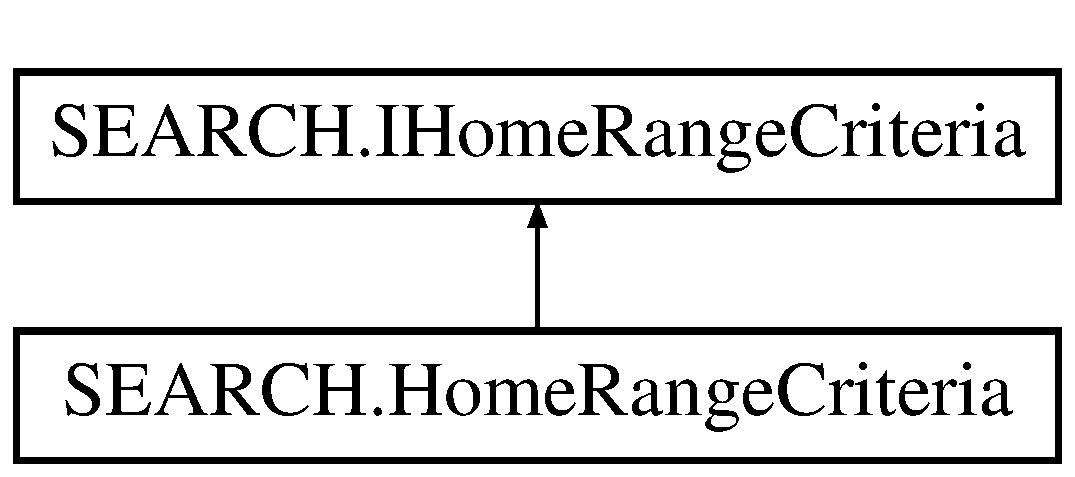
\includegraphics[height=2.000000cm]{class_s_e_a_r_c_h_1_1_home_range_criteria}
\end{center}
\end{figure}
\subsection*{Public Member Functions}
\begin{DoxyCompactItemize}
\item 
\hyperlink{class_s_e_a_r_c_h_1_1_home_range_criteria_a00f764a755326537e5c454f5e4f50b95}{Home\-Range\-Criteria} (double in\-Area, double in\-D\-M, double in\-D\-S\-D, double in\-D\-W)
\item 
\hyperlink{class_s_e_a_r_c_h_1_1_home_range_criteria_abc163593f3e7f29b83505a6fe2517c92}{Home\-Range\-Criteria} ()
\end{DoxyCompactItemize}
\subsection*{Properties}
\begin{DoxyCompactItemize}
\item 
double \hyperlink{class_s_e_a_r_c_h_1_1_home_range_criteria_a3d4caf6cd00810b53162b324d45edf02}{Area}\hspace{0.3cm}{\ttfamily  \mbox{[}get, set\mbox{]}}
\item 
double \hyperlink{class_s_e_a_r_c_h_1_1_home_range_criteria_afecf658def789f1220a0967c6ef26160}{Distance\-Mean}\hspace{0.3cm}{\ttfamily  \mbox{[}get, set\mbox{]}}
\item 
double \hyperlink{class_s_e_a_r_c_h_1_1_home_range_criteria_a3cae651fa48e552e6eec6f9fa8fcdb5e}{Distance\-S\-D}\hspace{0.3cm}{\ttfamily  \mbox{[}get, set\mbox{]}}
\item 
double \hyperlink{class_s_e_a_r_c_h_1_1_home_range_criteria_aa5642715adf3682f7dd16a1914dd92c3}{Distance\-Weight}\hspace{0.3cm}{\ttfamily  \mbox{[}get, set\mbox{]}}
\end{DoxyCompactItemize}


\subsection{Detailed Description}
contains the criteria for calculating the home range area 



\subsection{Constructor \& Destructor Documentation}
\hypertarget{class_s_e_a_r_c_h_1_1_home_range_criteria_a00f764a755326537e5c454f5e4f50b95}{\index{S\-E\-A\-R\-C\-H\-::\-Home\-Range\-Criteria@{S\-E\-A\-R\-C\-H\-::\-Home\-Range\-Criteria}!Home\-Range\-Criteria@{Home\-Range\-Criteria}}
\index{Home\-Range\-Criteria@{Home\-Range\-Criteria}!SEARCH::HomeRangeCriteria@{S\-E\-A\-R\-C\-H\-::\-Home\-Range\-Criteria}}
\subsubsection[{Home\-Range\-Criteria}]{\setlength{\rightskip}{0pt plus 5cm}S\-E\-A\-R\-C\-H.\-Home\-Range\-Criteria.\-Home\-Range\-Criteria (
\begin{DoxyParamCaption}
\item[{double}]{in\-Area, }
\item[{double}]{in\-D\-M, }
\item[{double}]{in\-D\-S\-D, }
\item[{double}]{in\-D\-W}
\end{DoxyParamCaption}
)}}\label{class_s_e_a_r_c_h_1_1_home_range_criteria_a00f764a755326537e5c454f5e4f50b95}
\hypertarget{class_s_e_a_r_c_h_1_1_home_range_criteria_abc163593f3e7f29b83505a6fe2517c92}{\index{S\-E\-A\-R\-C\-H\-::\-Home\-Range\-Criteria@{S\-E\-A\-R\-C\-H\-::\-Home\-Range\-Criteria}!Home\-Range\-Criteria@{Home\-Range\-Criteria}}
\index{Home\-Range\-Criteria@{Home\-Range\-Criteria}!SEARCH::HomeRangeCriteria@{S\-E\-A\-R\-C\-H\-::\-Home\-Range\-Criteria}}
\subsubsection[{Home\-Range\-Criteria}]{\setlength{\rightskip}{0pt plus 5cm}S\-E\-A\-R\-C\-H.\-Home\-Range\-Criteria.\-Home\-Range\-Criteria (
\begin{DoxyParamCaption}
{}
\end{DoxyParamCaption}
)}}\label{class_s_e_a_r_c_h_1_1_home_range_criteria_abc163593f3e7f29b83505a6fe2517c92}


\subsection{Property Documentation}
\hypertarget{class_s_e_a_r_c_h_1_1_home_range_criteria_a3d4caf6cd00810b53162b324d45edf02}{\index{S\-E\-A\-R\-C\-H\-::\-Home\-Range\-Criteria@{S\-E\-A\-R\-C\-H\-::\-Home\-Range\-Criteria}!Area@{Area}}
\index{Area@{Area}!SEARCH::HomeRangeCriteria@{S\-E\-A\-R\-C\-H\-::\-Home\-Range\-Criteria}}
\subsubsection[{Area}]{\setlength{\rightskip}{0pt plus 5cm}double S\-E\-A\-R\-C\-H.\-Home\-Range\-Criteria.\-Area\hspace{0.3cm}{\ttfamily [get]}, {\ttfamily [set]}}}\label{class_s_e_a_r_c_h_1_1_home_range_criteria_a3d4caf6cd00810b53162b324d45edf02}
\hypertarget{class_s_e_a_r_c_h_1_1_home_range_criteria_afecf658def789f1220a0967c6ef26160}{\index{S\-E\-A\-R\-C\-H\-::\-Home\-Range\-Criteria@{S\-E\-A\-R\-C\-H\-::\-Home\-Range\-Criteria}!Distance\-Mean@{Distance\-Mean}}
\index{Distance\-Mean@{Distance\-Mean}!SEARCH::HomeRangeCriteria@{S\-E\-A\-R\-C\-H\-::\-Home\-Range\-Criteria}}
\subsubsection[{Distance\-Mean}]{\setlength{\rightskip}{0pt plus 5cm}double S\-E\-A\-R\-C\-H.\-Home\-Range\-Criteria.\-Distance\-Mean\hspace{0.3cm}{\ttfamily [get]}, {\ttfamily [set]}}}\label{class_s_e_a_r_c_h_1_1_home_range_criteria_afecf658def789f1220a0967c6ef26160}
\hypertarget{class_s_e_a_r_c_h_1_1_home_range_criteria_a3cae651fa48e552e6eec6f9fa8fcdb5e}{\index{S\-E\-A\-R\-C\-H\-::\-Home\-Range\-Criteria@{S\-E\-A\-R\-C\-H\-::\-Home\-Range\-Criteria}!Distance\-S\-D@{Distance\-S\-D}}
\index{Distance\-S\-D@{Distance\-S\-D}!SEARCH::HomeRangeCriteria@{S\-E\-A\-R\-C\-H\-::\-Home\-Range\-Criteria}}
\subsubsection[{Distance\-S\-D}]{\setlength{\rightskip}{0pt plus 5cm}double S\-E\-A\-R\-C\-H.\-Home\-Range\-Criteria.\-Distance\-S\-D\hspace{0.3cm}{\ttfamily [get]}, {\ttfamily [set]}}}\label{class_s_e_a_r_c_h_1_1_home_range_criteria_a3cae651fa48e552e6eec6f9fa8fcdb5e}
\hypertarget{class_s_e_a_r_c_h_1_1_home_range_criteria_aa5642715adf3682f7dd16a1914dd92c3}{\index{S\-E\-A\-R\-C\-H\-::\-Home\-Range\-Criteria@{S\-E\-A\-R\-C\-H\-::\-Home\-Range\-Criteria}!Distance\-Weight@{Distance\-Weight}}
\index{Distance\-Weight@{Distance\-Weight}!SEARCH::HomeRangeCriteria@{S\-E\-A\-R\-C\-H\-::\-Home\-Range\-Criteria}}
\subsubsection[{Distance\-Weight}]{\setlength{\rightskip}{0pt plus 5cm}double S\-E\-A\-R\-C\-H.\-Home\-Range\-Criteria.\-Distance\-Weight\hspace{0.3cm}{\ttfamily [get]}, {\ttfamily [set]}}}\label{class_s_e_a_r_c_h_1_1_home_range_criteria_aa5642715adf3682f7dd16a1914dd92c3}


The documentation for this class was generated from the following file\-:\begin{DoxyCompactItemize}
\item 
Desktop/vlog4net\-A\-R\-C10\-\_\-64\-\_\-newhoming/\-Data\-Centric/\hyperlink{_home_range_criteria_8cs}{Home\-Range\-Criteria.\-cs}\end{DoxyCompactItemize}

\hypertarget{class_s_e_a_r_c_h_1_1_home_range_finder}{\section{S\-E\-A\-R\-C\-H.\-Home\-Range\-Finder Class Reference}
\label{class_s_e_a_r_c_h_1_1_home_range_finder}\index{S\-E\-A\-R\-C\-H.\-Home\-Range\-Finder@{S\-E\-A\-R\-C\-H.\-Home\-Range\-Finder}}
}


Summary description for \hyperlink{class_s_e_a_r_c_h_1_1_home_range_finder}{Home\-Range\-Finder}.  


Inheritance diagram for S\-E\-A\-R\-C\-H.\-Home\-Range\-Finder\-:\begin{figure}[H]
\begin{center}
\leavevmode
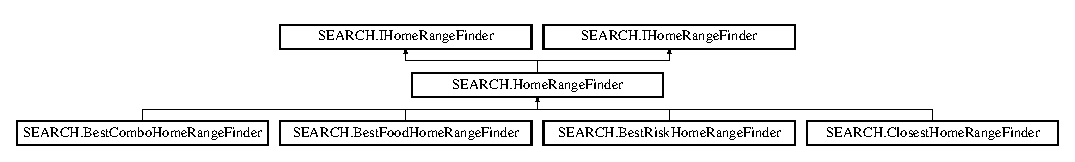
\includegraphics[height=1.728395cm]{class_s_e_a_r_c_h_1_1_home_range_finder}
\end{center}
\end{figure}
\subsection*{Public Member Functions}
\begin{DoxyCompactItemize}
\item 
virtual bool \hyperlink{class_s_e_a_r_c_h_1_1_home_range_finder_a1215e70b082e787d5dd87180641339a6}{set\-Home\-Range\-Center} (\hyperlink{class_s_e_a_r_c_h_1_1_animal}{Animal} in\-Animal, E\-S\-R\-I.\-Arc\-G\-I\-S.\-Geodatabase.\-I\-Feature\-Class in\-Anmial\-Memory\-Map)
\item 
virtual bool \hyperlink{class_s_e_a_r_c_h_1_1_home_range_finder_a41b187329b1cd89b91c9c2f4a145ec7b}{set\-Home\-Range\-Center} (\hyperlink{class_s_e_a_r_c_h_1_1_animal}{Animal} in\-A, string in\-File\-Name)
\item 
virtual bool \hyperlink{class_s_e_a_r_c_h_1_1_home_range_finder_a1215e70b082e787d5dd87180641339a6}{set\-Home\-Range\-Center} (\hyperlink{class_s_e_a_r_c_h_1_1_animal}{Animal} in\-Animal, E\-S\-R\-I.\-Arc\-G\-I\-S.\-Geodatabase.\-I\-Feature\-Class in\-Anmial\-Memory\-Map)
\item 
virtual bool \hyperlink{class_s_e_a_r_c_h_1_1_home_range_finder_a41b187329b1cd89b91c9c2f4a145ec7b}{set\-Home\-Range\-Center} (\hyperlink{class_s_e_a_r_c_h_1_1_animal}{Animal} in\-A, string in\-File\-Name)
\end{DoxyCompactItemize}
\subsection*{Protected Member Functions}
\begin{DoxyCompactItemize}
\item 
\hyperlink{class_s_e_a_r_c_h_1_1_home_range_finder_af8bbe5c80277c37b7ab5d52e3e3f9eee}{Home\-Range\-Finder} ()
\item 
void \hyperlink{class_s_e_a_r_c_h_1_1_home_range_finder_abad00bb4ab60d23d836ead95d47c9ab7}{build\-Logger} ()
\item 
I\-Point \hyperlink{class_s_e_a_r_c_h_1_1_home_range_finder_a3afdb5c57d8b28d3a73f664fa4a6aeff}{choose\-Home\-Range\-Center} (List$<$ \hyperlink{class_s_e_a_r_c_h_1_1_eligible_home_site}{Eligible\-Home\-Site} $>$ in\-Qualified\-Sites, double min\-Home\-Range\-Area)
\item 
double \hyperlink{class_s_e_a_r_c_h_1_1_home_range_finder_aa3f14f619622faed6d6a0a98478bdbbf}{get\-Area} (I\-Point in\-Point)
\item 
double \hyperlink{class_s_e_a_r_c_h_1_1_home_range_finder_a8421eb01daa296e355c8cb63d3dbed20}{get\-Area} (I\-Polygon in\-Poly)
\item 
I\-Point \hyperlink{class_s_e_a_r_c_h_1_1_home_range_finder_aaa80430fcd57c47337bef5edb34cedf7}{get\-Home\-Range\-Center} (\hyperlink{class_s_e_a_r_c_h_1_1_eligible_home_sites}{Eligible\-Home\-Sites} in\-Ehs)
\item 
I\-Polygon \hyperlink{class_s_e_a_r_c_h_1_1_home_range_finder_a802ad742ff286588d0986401b13a5260}{get\-Polygon} (I\-Point in\-Point)
\item 
I\-Feature\-Cursor \hyperlink{class_s_e_a_r_c_h_1_1_home_range_finder_ad2d3ef0b0f55957ebad25d0f2a395ed6}{get\-Suitable\-Polygons} (I\-Feature\-Class in\-Features)
\item 
void \hyperlink{class_s_e_a_r_c_h_1_1_home_range_finder_ae107836c253caf611d08be84d350ba38}{make\-Array\-Of\-Polygons} (I\-Feature\-Cursor in\-F\-C)
\item 
\hyperlink{class_s_e_a_r_c_h_1_1_i_point_list}{I\-Point\-List} \hyperlink{class_s_e_a_r_c_h_1_1_home_range_finder_a09c218455700f3edcfe230af423753d5}{make\-Point\-List} (\hyperlink{class_s_e_a_r_c_h_1_1_eligible_home_sites}{Eligible\-Home\-Sites} in\-Ehs)
\item 
void \hyperlink{class_s_e_a_r_c_h_1_1_home_range_finder_ac4489d478a6b1c80b706de156179b7a5}{set\-Distance} (\hyperlink{class_s_e_a_r_c_h_1_1_animal}{Animal} in\-A)
\item 
bool \hyperlink{class_s_e_a_r_c_h_1_1_home_range_finder_a9ef874a4eb49913a8ce79e47e5eddfaa}{set\-Suitable\-Sites} (\hyperlink{class_s_e_a_r_c_h_1_1_animal}{Animal} in\-A, string in\-File\-Name)
\item 
\hyperlink{class_s_e_a_r_c_h_1_1_home_range_finder_af8bbe5c80277c37b7ab5d52e3e3f9eee}{Home\-Range\-Finder} ()
\item 
I\-Point \hyperlink{class_s_e_a_r_c_h_1_1_home_range_finder_ad34badc3e0dcabffa119bf1e9be038b9}{choose\-Home\-Range\-Center} (List$<$ \hyperlink{class_s_e_a_r_c_h_1_1_eligible_home_site}{Eligible\-Home\-Site} $>$ in\-Qualified\-Sites, double in\-Home\-Range\-Area)
\item 
bool \hyperlink{class_s_e_a_r_c_h_1_1_home_range_finder_ad1f9637aff3aa6067ee1eada06bd517c}{Find\-Home\-Range} (\hyperlink{class_s_e_a_r_c_h_1_1_animal}{Animal} in\-Animal, string in\-File\-Name)
\item 
double \hyperlink{class_s_e_a_r_c_h_1_1_home_range_finder_aa3f14f619622faed6d6a0a98478bdbbf}{get\-Area} (I\-Point in\-Point)
\item 
double \hyperlink{class_s_e_a_r_c_h_1_1_home_range_finder_a8421eb01daa296e355c8cb63d3dbed20}{get\-Area} (I\-Polygon in\-Poly)
\item 
I\-Point \hyperlink{class_s_e_a_r_c_h_1_1_home_range_finder_a8b69d52498981e0c2d2134bdc19e9265}{get\-Home\-Range\-Center} ()
\item 
I\-Point \hyperlink{class_s_e_a_r_c_h_1_1_home_range_finder_aaa80430fcd57c47337bef5edb34cedf7}{get\-Home\-Range\-Center} (\hyperlink{class_s_e_a_r_c_h_1_1_eligible_home_sites}{Eligible\-Home\-Sites} in\-Ehs)
\item 
I\-Polygon \hyperlink{class_s_e_a_r_c_h_1_1_home_range_finder_a802ad742ff286588d0986401b13a5260}{get\-Polygon} (I\-Point in\-Point)
\item 
List$<$ \hyperlink{class_s_e_a_r_c_h_1_1_eligible_home_site}{Eligible\-Home\-Site} $>$ \hyperlink{class_s_e_a_r_c_h_1_1_home_range_finder_a54bf6f15adf45a9827209a91d286c897}{get\-Suitable\-Steps} (string in\-Animal\-Memory\-Map)
\item 
void \hyperlink{class_s_e_a_r_c_h_1_1_home_range_finder_ae107836c253caf611d08be84d350ba38}{make\-Array\-Of\-Polygons} (I\-Feature\-Cursor in\-F\-C)
\item 
\hyperlink{class_s_e_a_r_c_h_1_1_i_point_list}{I\-Point\-List} \hyperlink{class_s_e_a_r_c_h_1_1_home_range_finder_a09c218455700f3edcfe230af423753d5}{make\-Point\-List} (\hyperlink{class_s_e_a_r_c_h_1_1_eligible_home_sites}{Eligible\-Home\-Sites} in\-Ehs)
\item 
void \hyperlink{class_s_e_a_r_c_h_1_1_home_range_finder_aa8f3a0963d2f66e546597840d9219d89}{set\-Distance} (I\-Point curr\-Location)
\item 
void \hyperlink{class_s_e_a_r_c_h_1_1_home_range_finder_ac4489d478a6b1c80b706de156179b7a5}{set\-Distance} (\hyperlink{class_s_e_a_r_c_h_1_1_animal}{Animal} in\-A)
\item 
void \hyperlink{class_s_e_a_r_c_h_1_1_home_range_finder_a0e5f3941a7fa90911e6ea0c09a7b831b}{Set\-Ranges} (double in\-Value)
\item 
bool \hyperlink{class_s_e_a_r_c_h_1_1_home_range_finder_a62f36c07aadf699d7c10852b1b19d00d}{set\-Suitable\-Polygons} (double min\-Area\-Needed\-Overall, string in\-Animal\-Sex, string in\-Animal\-Memory\-Map)
\item 
bool \hyperlink{class_s_e_a_r_c_h_1_1_home_range_finder_a9ef874a4eb49913a8ce79e47e5eddfaa}{set\-Suitable\-Sites} (\hyperlink{class_s_e_a_r_c_h_1_1_animal}{Animal} in\-A, string in\-File\-Name)
\end{DoxyCompactItemize}
\subsection*{Protected Attributes}
\begin{DoxyCompactItemize}
\item 
File\-Writer.\-File\-Writer \hyperlink{class_s_e_a_r_c_h_1_1_home_range_finder_a7aa6fb5898f942e04a2a68ee52e64eca}{fw}
\item 
\hyperlink{class_s_e_a_r_c_h_1_1_random_numbers}{Random\-Numbers} \hyperlink{class_s_e_a_r_c_h_1_1_home_range_finder_a476c2c25a136fd672fbabde620fc21e7}{rn} = null
\item 
System.\-Collections.\-Array\-List \hyperlink{class_s_e_a_r_c_h_1_1_home_range_finder_a7699b693447c55c2ad1b4a33ed55e6c7}{my\-Polygons}
\item 
List$<$ \hyperlink{class_s_e_a_r_c_h_1_1_eligible_home_site}{Eligible\-Home\-Site} $>$ \hyperlink{class_s_e_a_r_c_h_1_1_home_range_finder_a7020eef24adbc1e3d96a79a91f32a70e}{site\-List}
\end{DoxyCompactItemize}


\subsection{Detailed Description}
Summary description for \hyperlink{class_s_e_a_r_c_h_1_1_home_range_finder}{Home\-Range\-Finder}. 



\subsection{Constructor \& Destructor Documentation}
\hypertarget{class_s_e_a_r_c_h_1_1_home_range_finder_af8bbe5c80277c37b7ab5d52e3e3f9eee}{\index{S\-E\-A\-R\-C\-H\-::\-Home\-Range\-Finder@{S\-E\-A\-R\-C\-H\-::\-Home\-Range\-Finder}!Home\-Range\-Finder@{Home\-Range\-Finder}}
\index{Home\-Range\-Finder@{Home\-Range\-Finder}!SEARCH::HomeRangeFinder@{S\-E\-A\-R\-C\-H\-::\-Home\-Range\-Finder}}
\subsubsection[{Home\-Range\-Finder}]{\setlength{\rightskip}{0pt plus 5cm}S\-E\-A\-R\-C\-H.\-Home\-Range\-Finder.\-Home\-Range\-Finder (
\begin{DoxyParamCaption}
{}
\end{DoxyParamCaption}
)\hspace{0.3cm}{\ttfamily [protected]}}}\label{class_s_e_a_r_c_h_1_1_home_range_finder_af8bbe5c80277c37b7ab5d52e3e3f9eee}
\hypertarget{class_s_e_a_r_c_h_1_1_home_range_finder_af8bbe5c80277c37b7ab5d52e3e3f9eee}{\index{S\-E\-A\-R\-C\-H\-::\-Home\-Range\-Finder@{S\-E\-A\-R\-C\-H\-::\-Home\-Range\-Finder}!Home\-Range\-Finder@{Home\-Range\-Finder}}
\index{Home\-Range\-Finder@{Home\-Range\-Finder}!SEARCH::HomeRangeFinder@{S\-E\-A\-R\-C\-H\-::\-Home\-Range\-Finder}}
\subsubsection[{Home\-Range\-Finder}]{\setlength{\rightskip}{0pt plus 5cm}S\-E\-A\-R\-C\-H.\-Home\-Range\-Finder.\-Home\-Range\-Finder (
\begin{DoxyParamCaption}
{}
\end{DoxyParamCaption}
)\hspace{0.3cm}{\ttfamily [protected]}}}\label{class_s_e_a_r_c_h_1_1_home_range_finder_af8bbe5c80277c37b7ab5d52e3e3f9eee}


\subsection{Member Function Documentation}
\hypertarget{class_s_e_a_r_c_h_1_1_home_range_finder_abad00bb4ab60d23d836ead95d47c9ab7}{\index{S\-E\-A\-R\-C\-H\-::\-Home\-Range\-Finder@{S\-E\-A\-R\-C\-H\-::\-Home\-Range\-Finder}!build\-Logger@{build\-Logger}}
\index{build\-Logger@{build\-Logger}!SEARCH::HomeRangeFinder@{S\-E\-A\-R\-C\-H\-::\-Home\-Range\-Finder}}
\subsubsection[{build\-Logger}]{\setlength{\rightskip}{0pt plus 5cm}void S\-E\-A\-R\-C\-H.\-Home\-Range\-Finder.\-build\-Logger (
\begin{DoxyParamCaption}
{}
\end{DoxyParamCaption}
)\hspace{0.3cm}{\ttfamily [protected]}}}\label{class_s_e_a_r_c_h_1_1_home_range_finder_abad00bb4ab60d23d836ead95d47c9ab7}
\hypertarget{class_s_e_a_r_c_h_1_1_home_range_finder_ad34badc3e0dcabffa119bf1e9be038b9}{\index{S\-E\-A\-R\-C\-H\-::\-Home\-Range\-Finder@{S\-E\-A\-R\-C\-H\-::\-Home\-Range\-Finder}!choose\-Home\-Range\-Center@{choose\-Home\-Range\-Center}}
\index{choose\-Home\-Range\-Center@{choose\-Home\-Range\-Center}!SEARCH::HomeRangeFinder@{S\-E\-A\-R\-C\-H\-::\-Home\-Range\-Finder}}
\subsubsection[{choose\-Home\-Range\-Center}]{\setlength{\rightskip}{0pt plus 5cm}I\-Point S\-E\-A\-R\-C\-H.\-Home\-Range\-Finder.\-choose\-Home\-Range\-Center (
\begin{DoxyParamCaption}
\item[{List$<$ {\bf Eligible\-Home\-Site} $>$}]{in\-Qualified\-Sites, }
\item[{double}]{in\-Home\-Range\-Area}
\end{DoxyParamCaption}
)\hspace{0.3cm}{\ttfamily [protected]}}}\label{class_s_e_a_r_c_h_1_1_home_range_finder_ad34badc3e0dcabffa119bf1e9be038b9}
\hypertarget{class_s_e_a_r_c_h_1_1_home_range_finder_a3afdb5c57d8b28d3a73f664fa4a6aeff}{\index{S\-E\-A\-R\-C\-H\-::\-Home\-Range\-Finder@{S\-E\-A\-R\-C\-H\-::\-Home\-Range\-Finder}!choose\-Home\-Range\-Center@{choose\-Home\-Range\-Center}}
\index{choose\-Home\-Range\-Center@{choose\-Home\-Range\-Center}!SEARCH::HomeRangeFinder@{S\-E\-A\-R\-C\-H\-::\-Home\-Range\-Finder}}
\subsubsection[{choose\-Home\-Range\-Center}]{\setlength{\rightskip}{0pt plus 5cm}I\-Point S\-E\-A\-R\-C\-H.\-Home\-Range\-Finder.\-choose\-Home\-Range\-Center (
\begin{DoxyParamCaption}
\item[{List$<$ {\bf Eligible\-Home\-Site} $>$}]{in\-Qualified\-Sites, }
\item[{double}]{min\-Home\-Range\-Area}
\end{DoxyParamCaption}
)\hspace{0.3cm}{\ttfamily [protected]}}}\label{class_s_e_a_r_c_h_1_1_home_range_finder_a3afdb5c57d8b28d3a73f664fa4a6aeff}
\hypertarget{class_s_e_a_r_c_h_1_1_home_range_finder_ad1f9637aff3aa6067ee1eada06bd517c}{\index{S\-E\-A\-R\-C\-H\-::\-Home\-Range\-Finder@{S\-E\-A\-R\-C\-H\-::\-Home\-Range\-Finder}!Find\-Home\-Range@{Find\-Home\-Range}}
\index{Find\-Home\-Range@{Find\-Home\-Range}!SEARCH::HomeRangeFinder@{S\-E\-A\-R\-C\-H\-::\-Home\-Range\-Finder}}
\subsubsection[{Find\-Home\-Range}]{\setlength{\rightskip}{0pt plus 5cm}bool S\-E\-A\-R\-C\-H.\-Home\-Range\-Finder.\-Find\-Home\-Range (
\begin{DoxyParamCaption}
\item[{{\bf Animal}}]{in\-Animal, }
\item[{string}]{in\-File\-Name}
\end{DoxyParamCaption}
)\hspace{0.3cm}{\ttfamily [protected]}}}\label{class_s_e_a_r_c_h_1_1_home_range_finder_ad1f9637aff3aa6067ee1eada06bd517c}
\hypertarget{class_s_e_a_r_c_h_1_1_home_range_finder_aa3f14f619622faed6d6a0a98478bdbbf}{\index{S\-E\-A\-R\-C\-H\-::\-Home\-Range\-Finder@{S\-E\-A\-R\-C\-H\-::\-Home\-Range\-Finder}!get\-Area@{get\-Area}}
\index{get\-Area@{get\-Area}!SEARCH::HomeRangeFinder@{S\-E\-A\-R\-C\-H\-::\-Home\-Range\-Finder}}
\subsubsection[{get\-Area}]{\setlength{\rightskip}{0pt plus 5cm}double S\-E\-A\-R\-C\-H.\-Home\-Range\-Finder.\-get\-Area (
\begin{DoxyParamCaption}
\item[{I\-Point}]{in\-Point}
\end{DoxyParamCaption}
)\hspace{0.3cm}{\ttfamily [protected]}}}\label{class_s_e_a_r_c_h_1_1_home_range_finder_aa3f14f619622faed6d6a0a98478bdbbf}
\hypertarget{class_s_e_a_r_c_h_1_1_home_range_finder_a8421eb01daa296e355c8cb63d3dbed20}{\index{S\-E\-A\-R\-C\-H\-::\-Home\-Range\-Finder@{S\-E\-A\-R\-C\-H\-::\-Home\-Range\-Finder}!get\-Area@{get\-Area}}
\index{get\-Area@{get\-Area}!SEARCH::HomeRangeFinder@{S\-E\-A\-R\-C\-H\-::\-Home\-Range\-Finder}}
\subsubsection[{get\-Area}]{\setlength{\rightskip}{0pt plus 5cm}double S\-E\-A\-R\-C\-H.\-Home\-Range\-Finder.\-get\-Area (
\begin{DoxyParamCaption}
\item[{I\-Polygon}]{in\-Poly}
\end{DoxyParamCaption}
)\hspace{0.3cm}{\ttfamily [protected]}}}\label{class_s_e_a_r_c_h_1_1_home_range_finder_a8421eb01daa296e355c8cb63d3dbed20}
\hypertarget{class_s_e_a_r_c_h_1_1_home_range_finder_aa3f14f619622faed6d6a0a98478bdbbf}{\index{S\-E\-A\-R\-C\-H\-::\-Home\-Range\-Finder@{S\-E\-A\-R\-C\-H\-::\-Home\-Range\-Finder}!get\-Area@{get\-Area}}
\index{get\-Area@{get\-Area}!SEARCH::HomeRangeFinder@{S\-E\-A\-R\-C\-H\-::\-Home\-Range\-Finder}}
\subsubsection[{get\-Area}]{\setlength{\rightskip}{0pt plus 5cm}double S\-E\-A\-R\-C\-H.\-Home\-Range\-Finder.\-get\-Area (
\begin{DoxyParamCaption}
\item[{I\-Point}]{in\-Point}
\end{DoxyParamCaption}
)\hspace{0.3cm}{\ttfamily [protected]}}}\label{class_s_e_a_r_c_h_1_1_home_range_finder_aa3f14f619622faed6d6a0a98478bdbbf}
\hypertarget{class_s_e_a_r_c_h_1_1_home_range_finder_a8421eb01daa296e355c8cb63d3dbed20}{\index{S\-E\-A\-R\-C\-H\-::\-Home\-Range\-Finder@{S\-E\-A\-R\-C\-H\-::\-Home\-Range\-Finder}!get\-Area@{get\-Area}}
\index{get\-Area@{get\-Area}!SEARCH::HomeRangeFinder@{S\-E\-A\-R\-C\-H\-::\-Home\-Range\-Finder}}
\subsubsection[{get\-Area}]{\setlength{\rightskip}{0pt plus 5cm}double S\-E\-A\-R\-C\-H.\-Home\-Range\-Finder.\-get\-Area (
\begin{DoxyParamCaption}
\item[{I\-Polygon}]{in\-Poly}
\end{DoxyParamCaption}
)\hspace{0.3cm}{\ttfamily [protected]}}}\label{class_s_e_a_r_c_h_1_1_home_range_finder_a8421eb01daa296e355c8cb63d3dbed20}
\hypertarget{class_s_e_a_r_c_h_1_1_home_range_finder_aaa80430fcd57c47337bef5edb34cedf7}{\index{S\-E\-A\-R\-C\-H\-::\-Home\-Range\-Finder@{S\-E\-A\-R\-C\-H\-::\-Home\-Range\-Finder}!get\-Home\-Range\-Center@{get\-Home\-Range\-Center}}
\index{get\-Home\-Range\-Center@{get\-Home\-Range\-Center}!SEARCH::HomeRangeFinder@{S\-E\-A\-R\-C\-H\-::\-Home\-Range\-Finder}}
\subsubsection[{get\-Home\-Range\-Center}]{\setlength{\rightskip}{0pt plus 5cm}I\-Point S\-E\-A\-R\-C\-H.\-Home\-Range\-Finder.\-get\-Home\-Range\-Center (
\begin{DoxyParamCaption}
\item[{{\bf Eligible\-Home\-Sites}}]{in\-Ehs}
\end{DoxyParamCaption}
)\hspace{0.3cm}{\ttfamily [protected]}}}\label{class_s_e_a_r_c_h_1_1_home_range_finder_aaa80430fcd57c47337bef5edb34cedf7}
\hypertarget{class_s_e_a_r_c_h_1_1_home_range_finder_a8b69d52498981e0c2d2134bdc19e9265}{\index{S\-E\-A\-R\-C\-H\-::\-Home\-Range\-Finder@{S\-E\-A\-R\-C\-H\-::\-Home\-Range\-Finder}!get\-Home\-Range\-Center@{get\-Home\-Range\-Center}}
\index{get\-Home\-Range\-Center@{get\-Home\-Range\-Center}!SEARCH::HomeRangeFinder@{S\-E\-A\-R\-C\-H\-::\-Home\-Range\-Finder}}
\subsubsection[{get\-Home\-Range\-Center}]{\setlength{\rightskip}{0pt plus 5cm}I\-Point S\-E\-A\-R\-C\-H.\-Home\-Range\-Finder.\-get\-Home\-Range\-Center (
\begin{DoxyParamCaption}
{}
\end{DoxyParamCaption}
)\hspace{0.3cm}{\ttfamily [protected]}}}\label{class_s_e_a_r_c_h_1_1_home_range_finder_a8b69d52498981e0c2d2134bdc19e9265}
\hypertarget{class_s_e_a_r_c_h_1_1_home_range_finder_aaa80430fcd57c47337bef5edb34cedf7}{\index{S\-E\-A\-R\-C\-H\-::\-Home\-Range\-Finder@{S\-E\-A\-R\-C\-H\-::\-Home\-Range\-Finder}!get\-Home\-Range\-Center@{get\-Home\-Range\-Center}}
\index{get\-Home\-Range\-Center@{get\-Home\-Range\-Center}!SEARCH::HomeRangeFinder@{S\-E\-A\-R\-C\-H\-::\-Home\-Range\-Finder}}
\subsubsection[{get\-Home\-Range\-Center}]{\setlength{\rightskip}{0pt plus 5cm}I\-Point S\-E\-A\-R\-C\-H.\-Home\-Range\-Finder.\-get\-Home\-Range\-Center (
\begin{DoxyParamCaption}
\item[{{\bf Eligible\-Home\-Sites}}]{in\-Ehs}
\end{DoxyParamCaption}
)\hspace{0.3cm}{\ttfamily [protected]}}}\label{class_s_e_a_r_c_h_1_1_home_range_finder_aaa80430fcd57c47337bef5edb34cedf7}
\hypertarget{class_s_e_a_r_c_h_1_1_home_range_finder_a802ad742ff286588d0986401b13a5260}{\index{S\-E\-A\-R\-C\-H\-::\-Home\-Range\-Finder@{S\-E\-A\-R\-C\-H\-::\-Home\-Range\-Finder}!get\-Polygon@{get\-Polygon}}
\index{get\-Polygon@{get\-Polygon}!SEARCH::HomeRangeFinder@{S\-E\-A\-R\-C\-H\-::\-Home\-Range\-Finder}}
\subsubsection[{get\-Polygon}]{\setlength{\rightskip}{0pt plus 5cm}I\-Polygon S\-E\-A\-R\-C\-H.\-Home\-Range\-Finder.\-get\-Polygon (
\begin{DoxyParamCaption}
\item[{I\-Point}]{in\-Point}
\end{DoxyParamCaption}
)\hspace{0.3cm}{\ttfamily [protected]}}}\label{class_s_e_a_r_c_h_1_1_home_range_finder_a802ad742ff286588d0986401b13a5260}
\hypertarget{class_s_e_a_r_c_h_1_1_home_range_finder_a802ad742ff286588d0986401b13a5260}{\index{S\-E\-A\-R\-C\-H\-::\-Home\-Range\-Finder@{S\-E\-A\-R\-C\-H\-::\-Home\-Range\-Finder}!get\-Polygon@{get\-Polygon}}
\index{get\-Polygon@{get\-Polygon}!SEARCH::HomeRangeFinder@{S\-E\-A\-R\-C\-H\-::\-Home\-Range\-Finder}}
\subsubsection[{get\-Polygon}]{\setlength{\rightskip}{0pt plus 5cm}I\-Polygon S\-E\-A\-R\-C\-H.\-Home\-Range\-Finder.\-get\-Polygon (
\begin{DoxyParamCaption}
\item[{I\-Point}]{in\-Point}
\end{DoxyParamCaption}
)\hspace{0.3cm}{\ttfamily [protected]}}}\label{class_s_e_a_r_c_h_1_1_home_range_finder_a802ad742ff286588d0986401b13a5260}
\hypertarget{class_s_e_a_r_c_h_1_1_home_range_finder_ad2d3ef0b0f55957ebad25d0f2a395ed6}{\index{S\-E\-A\-R\-C\-H\-::\-Home\-Range\-Finder@{S\-E\-A\-R\-C\-H\-::\-Home\-Range\-Finder}!get\-Suitable\-Polygons@{get\-Suitable\-Polygons}}
\index{get\-Suitable\-Polygons@{get\-Suitable\-Polygons}!SEARCH::HomeRangeFinder@{S\-E\-A\-R\-C\-H\-::\-Home\-Range\-Finder}}
\subsubsection[{get\-Suitable\-Polygons}]{\setlength{\rightskip}{0pt plus 5cm}I\-Feature\-Cursor S\-E\-A\-R\-C\-H.\-Home\-Range\-Finder.\-get\-Suitable\-Polygons (
\begin{DoxyParamCaption}
\item[{I\-Feature\-Class}]{in\-Features}
\end{DoxyParamCaption}
)\hspace{0.3cm}{\ttfamily [protected]}}}\label{class_s_e_a_r_c_h_1_1_home_range_finder_ad2d3ef0b0f55957ebad25d0f2a395ed6}
\hypertarget{class_s_e_a_r_c_h_1_1_home_range_finder_a54bf6f15adf45a9827209a91d286c897}{\index{S\-E\-A\-R\-C\-H\-::\-Home\-Range\-Finder@{S\-E\-A\-R\-C\-H\-::\-Home\-Range\-Finder}!get\-Suitable\-Steps@{get\-Suitable\-Steps}}
\index{get\-Suitable\-Steps@{get\-Suitable\-Steps}!SEARCH::HomeRangeFinder@{S\-E\-A\-R\-C\-H\-::\-Home\-Range\-Finder}}
\subsubsection[{get\-Suitable\-Steps}]{\setlength{\rightskip}{0pt plus 5cm}List$<${\bf Eligible\-Home\-Site}$>$ S\-E\-A\-R\-C\-H.\-Home\-Range\-Finder.\-get\-Suitable\-Steps (
\begin{DoxyParamCaption}
\item[{string}]{in\-Animal\-Memory\-Map}
\end{DoxyParamCaption}
)\hspace{0.3cm}{\ttfamily [protected]}}}\label{class_s_e_a_r_c_h_1_1_home_range_finder_a54bf6f15adf45a9827209a91d286c897}
\hypertarget{class_s_e_a_r_c_h_1_1_home_range_finder_ae107836c253caf611d08be84d350ba38}{\index{S\-E\-A\-R\-C\-H\-::\-Home\-Range\-Finder@{S\-E\-A\-R\-C\-H\-::\-Home\-Range\-Finder}!make\-Array\-Of\-Polygons@{make\-Array\-Of\-Polygons}}
\index{make\-Array\-Of\-Polygons@{make\-Array\-Of\-Polygons}!SEARCH::HomeRangeFinder@{S\-E\-A\-R\-C\-H\-::\-Home\-Range\-Finder}}
\subsubsection[{make\-Array\-Of\-Polygons}]{\setlength{\rightskip}{0pt plus 5cm}void S\-E\-A\-R\-C\-H.\-Home\-Range\-Finder.\-make\-Array\-Of\-Polygons (
\begin{DoxyParamCaption}
\item[{I\-Feature\-Cursor}]{in\-F\-C}
\end{DoxyParamCaption}
)\hspace{0.3cm}{\ttfamily [protected]}}}\label{class_s_e_a_r_c_h_1_1_home_range_finder_ae107836c253caf611d08be84d350ba38}
\hypertarget{class_s_e_a_r_c_h_1_1_home_range_finder_ae107836c253caf611d08be84d350ba38}{\index{S\-E\-A\-R\-C\-H\-::\-Home\-Range\-Finder@{S\-E\-A\-R\-C\-H\-::\-Home\-Range\-Finder}!make\-Array\-Of\-Polygons@{make\-Array\-Of\-Polygons}}
\index{make\-Array\-Of\-Polygons@{make\-Array\-Of\-Polygons}!SEARCH::HomeRangeFinder@{S\-E\-A\-R\-C\-H\-::\-Home\-Range\-Finder}}
\subsubsection[{make\-Array\-Of\-Polygons}]{\setlength{\rightskip}{0pt plus 5cm}void S\-E\-A\-R\-C\-H.\-Home\-Range\-Finder.\-make\-Array\-Of\-Polygons (
\begin{DoxyParamCaption}
\item[{I\-Feature\-Cursor}]{in\-F\-C}
\end{DoxyParamCaption}
)\hspace{0.3cm}{\ttfamily [protected]}}}\label{class_s_e_a_r_c_h_1_1_home_range_finder_ae107836c253caf611d08be84d350ba38}
\hypertarget{class_s_e_a_r_c_h_1_1_home_range_finder_a09c218455700f3edcfe230af423753d5}{\index{S\-E\-A\-R\-C\-H\-::\-Home\-Range\-Finder@{S\-E\-A\-R\-C\-H\-::\-Home\-Range\-Finder}!make\-Point\-List@{make\-Point\-List}}
\index{make\-Point\-List@{make\-Point\-List}!SEARCH::HomeRangeFinder@{S\-E\-A\-R\-C\-H\-::\-Home\-Range\-Finder}}
\subsubsection[{make\-Point\-List}]{\setlength{\rightskip}{0pt plus 5cm}{\bf I\-Point\-List} S\-E\-A\-R\-C\-H.\-Home\-Range\-Finder.\-make\-Point\-List (
\begin{DoxyParamCaption}
\item[{{\bf Eligible\-Home\-Sites}}]{in\-Ehs}
\end{DoxyParamCaption}
)\hspace{0.3cm}{\ttfamily [protected]}}}\label{class_s_e_a_r_c_h_1_1_home_range_finder_a09c218455700f3edcfe230af423753d5}
\hypertarget{class_s_e_a_r_c_h_1_1_home_range_finder_a09c218455700f3edcfe230af423753d5}{\index{S\-E\-A\-R\-C\-H\-::\-Home\-Range\-Finder@{S\-E\-A\-R\-C\-H\-::\-Home\-Range\-Finder}!make\-Point\-List@{make\-Point\-List}}
\index{make\-Point\-List@{make\-Point\-List}!SEARCH::HomeRangeFinder@{S\-E\-A\-R\-C\-H\-::\-Home\-Range\-Finder}}
\subsubsection[{make\-Point\-List}]{\setlength{\rightskip}{0pt plus 5cm}{\bf I\-Point\-List} S\-E\-A\-R\-C\-H.\-Home\-Range\-Finder.\-make\-Point\-List (
\begin{DoxyParamCaption}
\item[{{\bf Eligible\-Home\-Sites}}]{in\-Ehs}
\end{DoxyParamCaption}
)\hspace{0.3cm}{\ttfamily [protected]}}}\label{class_s_e_a_r_c_h_1_1_home_range_finder_a09c218455700f3edcfe230af423753d5}
\hypertarget{class_s_e_a_r_c_h_1_1_home_range_finder_ac4489d478a6b1c80b706de156179b7a5}{\index{S\-E\-A\-R\-C\-H\-::\-Home\-Range\-Finder@{S\-E\-A\-R\-C\-H\-::\-Home\-Range\-Finder}!set\-Distance@{set\-Distance}}
\index{set\-Distance@{set\-Distance}!SEARCH::HomeRangeFinder@{S\-E\-A\-R\-C\-H\-::\-Home\-Range\-Finder}}
\subsubsection[{set\-Distance}]{\setlength{\rightskip}{0pt plus 5cm}void S\-E\-A\-R\-C\-H.\-Home\-Range\-Finder.\-set\-Distance (
\begin{DoxyParamCaption}
\item[{{\bf Animal}}]{in\-A}
\end{DoxyParamCaption}
)\hspace{0.3cm}{\ttfamily [protected]}}}\label{class_s_e_a_r_c_h_1_1_home_range_finder_ac4489d478a6b1c80b706de156179b7a5}
\hypertarget{class_s_e_a_r_c_h_1_1_home_range_finder_aa8f3a0963d2f66e546597840d9219d89}{\index{S\-E\-A\-R\-C\-H\-::\-Home\-Range\-Finder@{S\-E\-A\-R\-C\-H\-::\-Home\-Range\-Finder}!set\-Distance@{set\-Distance}}
\index{set\-Distance@{set\-Distance}!SEARCH::HomeRangeFinder@{S\-E\-A\-R\-C\-H\-::\-Home\-Range\-Finder}}
\subsubsection[{set\-Distance}]{\setlength{\rightskip}{0pt plus 5cm}void S\-E\-A\-R\-C\-H.\-Home\-Range\-Finder.\-set\-Distance (
\begin{DoxyParamCaption}
\item[{I\-Point}]{curr\-Location}
\end{DoxyParamCaption}
)\hspace{0.3cm}{\ttfamily [protected]}}}\label{class_s_e_a_r_c_h_1_1_home_range_finder_aa8f3a0963d2f66e546597840d9219d89}
\hypertarget{class_s_e_a_r_c_h_1_1_home_range_finder_ac4489d478a6b1c80b706de156179b7a5}{\index{S\-E\-A\-R\-C\-H\-::\-Home\-Range\-Finder@{S\-E\-A\-R\-C\-H\-::\-Home\-Range\-Finder}!set\-Distance@{set\-Distance}}
\index{set\-Distance@{set\-Distance}!SEARCH::HomeRangeFinder@{S\-E\-A\-R\-C\-H\-::\-Home\-Range\-Finder}}
\subsubsection[{set\-Distance}]{\setlength{\rightskip}{0pt plus 5cm}void S\-E\-A\-R\-C\-H.\-Home\-Range\-Finder.\-set\-Distance (
\begin{DoxyParamCaption}
\item[{{\bf Animal}}]{in\-A}
\end{DoxyParamCaption}
)\hspace{0.3cm}{\ttfamily [protected]}}}\label{class_s_e_a_r_c_h_1_1_home_range_finder_ac4489d478a6b1c80b706de156179b7a5}
\hypertarget{class_s_e_a_r_c_h_1_1_home_range_finder_a1215e70b082e787d5dd87180641339a6}{\index{S\-E\-A\-R\-C\-H\-::\-Home\-Range\-Finder@{S\-E\-A\-R\-C\-H\-::\-Home\-Range\-Finder}!set\-Home\-Range\-Center@{set\-Home\-Range\-Center}}
\index{set\-Home\-Range\-Center@{set\-Home\-Range\-Center}!SEARCH::HomeRangeFinder@{S\-E\-A\-R\-C\-H\-::\-Home\-Range\-Finder}}
\subsubsection[{set\-Home\-Range\-Center}]{\setlength{\rightskip}{0pt plus 5cm}virtual bool S\-E\-A\-R\-C\-H.\-Home\-Range\-Finder.\-set\-Home\-Range\-Center (
\begin{DoxyParamCaption}
\item[{{\bf Animal}}]{in\-Animal, }
\item[{E\-S\-R\-I.\-Arc\-G\-I\-S.\-Geodatabase.\-I\-Feature\-Class}]{in\-Anmial\-Memory\-Map}
\end{DoxyParamCaption}
)\hspace{0.3cm}{\ttfamily [virtual]}}}\label{class_s_e_a_r_c_h_1_1_home_range_finder_a1215e70b082e787d5dd87180641339a6}
\hypertarget{class_s_e_a_r_c_h_1_1_home_range_finder_a41b187329b1cd89b91c9c2f4a145ec7b}{\index{S\-E\-A\-R\-C\-H\-::\-Home\-Range\-Finder@{S\-E\-A\-R\-C\-H\-::\-Home\-Range\-Finder}!set\-Home\-Range\-Center@{set\-Home\-Range\-Center}}
\index{set\-Home\-Range\-Center@{set\-Home\-Range\-Center}!SEARCH::HomeRangeFinder@{S\-E\-A\-R\-C\-H\-::\-Home\-Range\-Finder}}
\subsubsection[{set\-Home\-Range\-Center}]{\setlength{\rightskip}{0pt plus 5cm}virtual bool S\-E\-A\-R\-C\-H.\-Home\-Range\-Finder.\-set\-Home\-Range\-Center (
\begin{DoxyParamCaption}
\item[{{\bf Animal}}]{in\-A, }
\item[{string}]{in\-File\-Name}
\end{DoxyParamCaption}
)\hspace{0.3cm}{\ttfamily [virtual]}}}\label{class_s_e_a_r_c_h_1_1_home_range_finder_a41b187329b1cd89b91c9c2f4a145ec7b}


Implements \hyperlink{interface_s_e_a_r_c_h_1_1_i_home_range_finder_a826e9e604bb2f25077d4896464f225a1}{S\-E\-A\-R\-C\-H.\-I\-Home\-Range\-Finder}.



Reimplemented in \hyperlink{class_s_e_a_r_c_h_1_1_best_food_home_range_finder_aa9876f866a2bc8ffca635caafb20add3}{S\-E\-A\-R\-C\-H.\-Best\-Food\-Home\-Range\-Finder}, \hyperlink{class_s_e_a_r_c_h_1_1_best_combo_home_range_finder_a3ea0071e375fca09e9116bf627e205b5}{S\-E\-A\-R\-C\-H.\-Best\-Combo\-Home\-Range\-Finder}, \hyperlink{class_s_e_a_r_c_h_1_1_best_risk_home_range_finder_a90867156ad508254624d441fb9116d65}{S\-E\-A\-R\-C\-H.\-Best\-Risk\-Home\-Range\-Finder}, and \hyperlink{class_s_e_a_r_c_h_1_1_closest_home_range_finder_a9f4b1aae4a27e1109c03ea444fdaf185}{S\-E\-A\-R\-C\-H.\-Closest\-Home\-Range\-Finder}.

\hypertarget{class_s_e_a_r_c_h_1_1_home_range_finder_a1215e70b082e787d5dd87180641339a6}{\index{S\-E\-A\-R\-C\-H\-::\-Home\-Range\-Finder@{S\-E\-A\-R\-C\-H\-::\-Home\-Range\-Finder}!set\-Home\-Range\-Center@{set\-Home\-Range\-Center}}
\index{set\-Home\-Range\-Center@{set\-Home\-Range\-Center}!SEARCH::HomeRangeFinder@{S\-E\-A\-R\-C\-H\-::\-Home\-Range\-Finder}}
\subsubsection[{set\-Home\-Range\-Center}]{\setlength{\rightskip}{0pt plus 5cm}virtual bool S\-E\-A\-R\-C\-H.\-Home\-Range\-Finder.\-set\-Home\-Range\-Center (
\begin{DoxyParamCaption}
\item[{{\bf Animal}}]{in\-Animal, }
\item[{E\-S\-R\-I.\-Arc\-G\-I\-S.\-Geodatabase.\-I\-Feature\-Class}]{in\-Anmial\-Memory\-Map}
\end{DoxyParamCaption}
)\hspace{0.3cm}{\ttfamily [virtual]}}}\label{class_s_e_a_r_c_h_1_1_home_range_finder_a1215e70b082e787d5dd87180641339a6}
\hypertarget{class_s_e_a_r_c_h_1_1_home_range_finder_a41b187329b1cd89b91c9c2f4a145ec7b}{\index{S\-E\-A\-R\-C\-H\-::\-Home\-Range\-Finder@{S\-E\-A\-R\-C\-H\-::\-Home\-Range\-Finder}!set\-Home\-Range\-Center@{set\-Home\-Range\-Center}}
\index{set\-Home\-Range\-Center@{set\-Home\-Range\-Center}!SEARCH::HomeRangeFinder@{S\-E\-A\-R\-C\-H\-::\-Home\-Range\-Finder}}
\subsubsection[{set\-Home\-Range\-Center}]{\setlength{\rightskip}{0pt plus 5cm}virtual bool S\-E\-A\-R\-C\-H.\-Home\-Range\-Finder.\-set\-Home\-Range\-Center (
\begin{DoxyParamCaption}
\item[{{\bf Animal}}]{in\-A, }
\item[{string}]{in\-File\-Name}
\end{DoxyParamCaption}
)\hspace{0.3cm}{\ttfamily [virtual]}}}\label{class_s_e_a_r_c_h_1_1_home_range_finder_a41b187329b1cd89b91c9c2f4a145ec7b}


Implements \hyperlink{interface_s_e_a_r_c_h_1_1_i_home_range_finder_a826e9e604bb2f25077d4896464f225a1}{S\-E\-A\-R\-C\-H.\-I\-Home\-Range\-Finder}.



Reimplemented in \hyperlink{class_s_e_a_r_c_h_1_1_best_food_home_range_finder_aa9876f866a2bc8ffca635caafb20add3}{S\-E\-A\-R\-C\-H.\-Best\-Food\-Home\-Range\-Finder}, \hyperlink{class_s_e_a_r_c_h_1_1_best_combo_home_range_finder_a3ea0071e375fca09e9116bf627e205b5}{S\-E\-A\-R\-C\-H.\-Best\-Combo\-Home\-Range\-Finder}, \hyperlink{class_s_e_a_r_c_h_1_1_best_risk_home_range_finder_a90867156ad508254624d441fb9116d65}{S\-E\-A\-R\-C\-H.\-Best\-Risk\-Home\-Range\-Finder}, and \hyperlink{class_s_e_a_r_c_h_1_1_closest_home_range_finder_a9f4b1aae4a27e1109c03ea444fdaf185}{S\-E\-A\-R\-C\-H.\-Closest\-Home\-Range\-Finder}.

\hypertarget{class_s_e_a_r_c_h_1_1_home_range_finder_a0e5f3941a7fa90911e6ea0c09a7b831b}{\index{S\-E\-A\-R\-C\-H\-::\-Home\-Range\-Finder@{S\-E\-A\-R\-C\-H\-::\-Home\-Range\-Finder}!Set\-Ranges@{Set\-Ranges}}
\index{Set\-Ranges@{Set\-Ranges}!SEARCH::HomeRangeFinder@{S\-E\-A\-R\-C\-H\-::\-Home\-Range\-Finder}}
\subsubsection[{Set\-Ranges}]{\setlength{\rightskip}{0pt plus 5cm}void S\-E\-A\-R\-C\-H.\-Home\-Range\-Finder.\-Set\-Ranges (
\begin{DoxyParamCaption}
\item[{double}]{in\-Value}
\end{DoxyParamCaption}
)\hspace{0.3cm}{\ttfamily [protected]}}}\label{class_s_e_a_r_c_h_1_1_home_range_finder_a0e5f3941a7fa90911e6ea0c09a7b831b}
\hypertarget{class_s_e_a_r_c_h_1_1_home_range_finder_a62f36c07aadf699d7c10852b1b19d00d}{\index{S\-E\-A\-R\-C\-H\-::\-Home\-Range\-Finder@{S\-E\-A\-R\-C\-H\-::\-Home\-Range\-Finder}!set\-Suitable\-Polygons@{set\-Suitable\-Polygons}}
\index{set\-Suitable\-Polygons@{set\-Suitable\-Polygons}!SEARCH::HomeRangeFinder@{S\-E\-A\-R\-C\-H\-::\-Home\-Range\-Finder}}
\subsubsection[{set\-Suitable\-Polygons}]{\setlength{\rightskip}{0pt plus 5cm}bool S\-E\-A\-R\-C\-H.\-Home\-Range\-Finder.\-set\-Suitable\-Polygons (
\begin{DoxyParamCaption}
\item[{double}]{min\-Area\-Needed\-Overall, }
\item[{string}]{in\-Animal\-Sex, }
\item[{string}]{in\-Animal\-Memory\-Map}
\end{DoxyParamCaption}
)\hspace{0.3cm}{\ttfamily [protected]}}}\label{class_s_e_a_r_c_h_1_1_home_range_finder_a62f36c07aadf699d7c10852b1b19d00d}
\hypertarget{class_s_e_a_r_c_h_1_1_home_range_finder_a9ef874a4eb49913a8ce79e47e5eddfaa}{\index{S\-E\-A\-R\-C\-H\-::\-Home\-Range\-Finder@{S\-E\-A\-R\-C\-H\-::\-Home\-Range\-Finder}!set\-Suitable\-Sites@{set\-Suitable\-Sites}}
\index{set\-Suitable\-Sites@{set\-Suitable\-Sites}!SEARCH::HomeRangeFinder@{S\-E\-A\-R\-C\-H\-::\-Home\-Range\-Finder}}
\subsubsection[{set\-Suitable\-Sites}]{\setlength{\rightskip}{0pt plus 5cm}bool S\-E\-A\-R\-C\-H.\-Home\-Range\-Finder.\-set\-Suitable\-Sites (
\begin{DoxyParamCaption}
\item[{{\bf Animal}}]{in\-A, }
\item[{string}]{in\-File\-Name}
\end{DoxyParamCaption}
)\hspace{0.3cm}{\ttfamily [protected]}}}\label{class_s_e_a_r_c_h_1_1_home_range_finder_a9ef874a4eb49913a8ce79e47e5eddfaa}
\hypertarget{class_s_e_a_r_c_h_1_1_home_range_finder_a9ef874a4eb49913a8ce79e47e5eddfaa}{\index{S\-E\-A\-R\-C\-H\-::\-Home\-Range\-Finder@{S\-E\-A\-R\-C\-H\-::\-Home\-Range\-Finder}!set\-Suitable\-Sites@{set\-Suitable\-Sites}}
\index{set\-Suitable\-Sites@{set\-Suitable\-Sites}!SEARCH::HomeRangeFinder@{S\-E\-A\-R\-C\-H\-::\-Home\-Range\-Finder}}
\subsubsection[{set\-Suitable\-Sites}]{\setlength{\rightskip}{0pt plus 5cm}bool S\-E\-A\-R\-C\-H.\-Home\-Range\-Finder.\-set\-Suitable\-Sites (
\begin{DoxyParamCaption}
\item[{{\bf Animal}}]{in\-A, }
\item[{string}]{in\-File\-Name}
\end{DoxyParamCaption}
)\hspace{0.3cm}{\ttfamily [protected]}}}\label{class_s_e_a_r_c_h_1_1_home_range_finder_a9ef874a4eb49913a8ce79e47e5eddfaa}


\subsection{Member Data Documentation}
\hypertarget{class_s_e_a_r_c_h_1_1_home_range_finder_a7aa6fb5898f942e04a2a68ee52e64eca}{\index{S\-E\-A\-R\-C\-H\-::\-Home\-Range\-Finder@{S\-E\-A\-R\-C\-H\-::\-Home\-Range\-Finder}!fw@{fw}}
\index{fw@{fw}!SEARCH::HomeRangeFinder@{S\-E\-A\-R\-C\-H\-::\-Home\-Range\-Finder}}
\subsubsection[{fw}]{\setlength{\rightskip}{0pt plus 5cm}File\-Writer.\-File\-Writer S\-E\-A\-R\-C\-H.\-Home\-Range\-Finder.\-fw\hspace{0.3cm}{\ttfamily [protected]}}}\label{class_s_e_a_r_c_h_1_1_home_range_finder_a7aa6fb5898f942e04a2a68ee52e64eca}
\hypertarget{class_s_e_a_r_c_h_1_1_home_range_finder_a7699b693447c55c2ad1b4a33ed55e6c7}{\index{S\-E\-A\-R\-C\-H\-::\-Home\-Range\-Finder@{S\-E\-A\-R\-C\-H\-::\-Home\-Range\-Finder}!my\-Polygons@{my\-Polygons}}
\index{my\-Polygons@{my\-Polygons}!SEARCH::HomeRangeFinder@{S\-E\-A\-R\-C\-H\-::\-Home\-Range\-Finder}}
\subsubsection[{my\-Polygons}]{\setlength{\rightskip}{0pt plus 5cm}System Collections Array\-List S\-E\-A\-R\-C\-H.\-Home\-Range\-Finder.\-my\-Polygons\hspace{0.3cm}{\ttfamily [protected]}}}\label{class_s_e_a_r_c_h_1_1_home_range_finder_a7699b693447c55c2ad1b4a33ed55e6c7}
\hypertarget{class_s_e_a_r_c_h_1_1_home_range_finder_a476c2c25a136fd672fbabde620fc21e7}{\index{S\-E\-A\-R\-C\-H\-::\-Home\-Range\-Finder@{S\-E\-A\-R\-C\-H\-::\-Home\-Range\-Finder}!rn@{rn}}
\index{rn@{rn}!SEARCH::HomeRangeFinder@{S\-E\-A\-R\-C\-H\-::\-Home\-Range\-Finder}}
\subsubsection[{rn}]{\setlength{\rightskip}{0pt plus 5cm}{\bf Random\-Numbers} S\-E\-A\-R\-C\-H.\-Home\-Range\-Finder.\-rn = null\hspace{0.3cm}{\ttfamily [protected]}}}\label{class_s_e_a_r_c_h_1_1_home_range_finder_a476c2c25a136fd672fbabde620fc21e7}
\hypertarget{class_s_e_a_r_c_h_1_1_home_range_finder_a7020eef24adbc1e3d96a79a91f32a70e}{\index{S\-E\-A\-R\-C\-H\-::\-Home\-Range\-Finder@{S\-E\-A\-R\-C\-H\-::\-Home\-Range\-Finder}!site\-List@{site\-List}}
\index{site\-List@{site\-List}!SEARCH::HomeRangeFinder@{S\-E\-A\-R\-C\-H\-::\-Home\-Range\-Finder}}
\subsubsection[{site\-List}]{\setlength{\rightskip}{0pt plus 5cm}List$<${\bf Eligible\-Home\-Site}$>$ S\-E\-A\-R\-C\-H.\-Home\-Range\-Finder.\-site\-List\hspace{0.3cm}{\ttfamily [protected]}}}\label{class_s_e_a_r_c_h_1_1_home_range_finder_a7020eef24adbc1e3d96a79a91f32a70e}


The documentation for this class was generated from the following files\-:\begin{DoxyCompactItemize}
\item 
Desktop/vlog4net\-A\-R\-C10\-\_\-64\-\_\-newhoming/\-Data\-Centric/\hyperlink{_home_range_finder_01-_01_copy_8cs}{Home\-Range\-Finder -\/ Copy.\-cs}\item 
Desktop/vlog4net\-A\-R\-C10\-\_\-64\-\_\-newhoming/\-Data\-Centric/\hyperlink{_home_range_finder_8cs}{Home\-Range\-Finder.\-cs}\end{DoxyCompactItemize}

\hypertarget{class_s_e_a_r_c_h_1_1_hourly_modifier}{\section{S\-E\-A\-R\-C\-H.\-Hourly\-Modifier Class Reference}
\label{class_s_e_a_r_c_h_1_1_hourly_modifier}\index{S\-E\-A\-R\-C\-H.\-Hourly\-Modifier@{S\-E\-A\-R\-C\-H.\-Hourly\-Modifier}}
}


Summary description for \hyperlink{class_s_e_a_r_c_h_1_1_hourly_modifier}{Hourly\-Modifier}.  


Inheritance diagram for S\-E\-A\-R\-C\-H.\-Hourly\-Modifier\-:\begin{figure}[H]
\begin{center}
\leavevmode
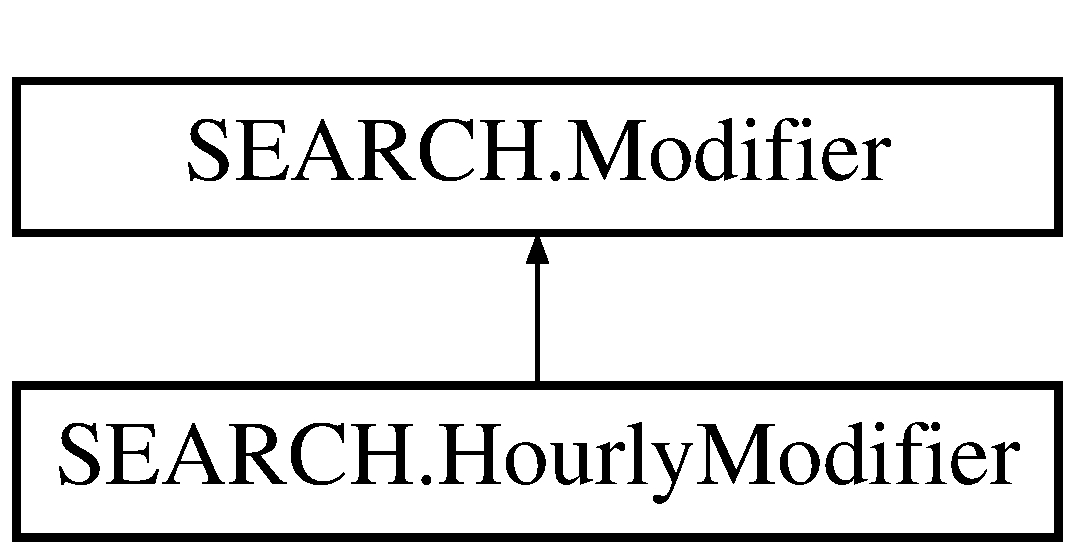
\includegraphics[height=2.000000cm]{class_s_e_a_r_c_h_1_1_hourly_modifier}
\end{center}
\end{figure}
\subsection*{Public Member Functions}
\begin{DoxyCompactItemize}
\item 
\hyperlink{class_s_e_a_r_c_h_1_1_hourly_modifier_a90843d950db0197f9ef151fabbc8fe42}{Hourly\-Modifier} ()
\end{DoxyCompactItemize}
\subsection*{Properties}
\begin{DoxyCompactItemize}
\item 
int \hyperlink{class_s_e_a_r_c_h_1_1_hourly_modifier_a2b71dd8284a1adbe21f5831522240497}{Start\-Time}\hspace{0.3cm}{\ttfamily  \mbox{[}get, set\mbox{]}}
\end{DoxyCompactItemize}


\subsection{Detailed Description}
Summary description for \hyperlink{class_s_e_a_r_c_h_1_1_hourly_modifier}{Hourly\-Modifier}. 



\subsection{Constructor \& Destructor Documentation}
\hypertarget{class_s_e_a_r_c_h_1_1_hourly_modifier_a90843d950db0197f9ef151fabbc8fe42}{\index{S\-E\-A\-R\-C\-H\-::\-Hourly\-Modifier@{S\-E\-A\-R\-C\-H\-::\-Hourly\-Modifier}!Hourly\-Modifier@{Hourly\-Modifier}}
\index{Hourly\-Modifier@{Hourly\-Modifier}!SEARCH::HourlyModifier@{S\-E\-A\-R\-C\-H\-::\-Hourly\-Modifier}}
\subsubsection[{Hourly\-Modifier}]{\setlength{\rightskip}{0pt plus 5cm}S\-E\-A\-R\-C\-H.\-Hourly\-Modifier.\-Hourly\-Modifier (
\begin{DoxyParamCaption}
{}
\end{DoxyParamCaption}
)}}\label{class_s_e_a_r_c_h_1_1_hourly_modifier_a90843d950db0197f9ef151fabbc8fe42}


\subsection{Property Documentation}
\hypertarget{class_s_e_a_r_c_h_1_1_hourly_modifier_a2b71dd8284a1adbe21f5831522240497}{\index{S\-E\-A\-R\-C\-H\-::\-Hourly\-Modifier@{S\-E\-A\-R\-C\-H\-::\-Hourly\-Modifier}!Start\-Time@{Start\-Time}}
\index{Start\-Time@{Start\-Time}!SEARCH::HourlyModifier@{S\-E\-A\-R\-C\-H\-::\-Hourly\-Modifier}}
\subsubsection[{Start\-Time}]{\setlength{\rightskip}{0pt plus 5cm}int S\-E\-A\-R\-C\-H.\-Hourly\-Modifier.\-Start\-Time\hspace{0.3cm}{\ttfamily [get]}, {\ttfamily [set]}}}\label{class_s_e_a_r_c_h_1_1_hourly_modifier_a2b71dd8284a1adbe21f5831522240497}


The documentation for this class was generated from the following file\-:\begin{DoxyCompactItemize}
\item 
Desktop/vlog4net\-A\-R\-C10\-\_\-64\-\_\-newhoming/\-Data\-Centric/\hyperlink{_hourly_modifier_8cs}{Hourly\-Modifier.\-cs}\end{DoxyCompactItemize}

\hypertarget{class_s_e_a_r_c_h_1_1_hourly_modifier_collection}{\section{S\-E\-A\-R\-C\-H.\-Hourly\-Modifier\-Collection Class Reference}
\label{class_s_e_a_r_c_h_1_1_hourly_modifier_collection}\index{S\-E\-A\-R\-C\-H.\-Hourly\-Modifier\-Collection@{S\-E\-A\-R\-C\-H.\-Hourly\-Modifier\-Collection}}
}
Inheritance diagram for S\-E\-A\-R\-C\-H.\-Hourly\-Modifier\-Collection\-:\begin{figure}[H]
\begin{center}
\leavevmode
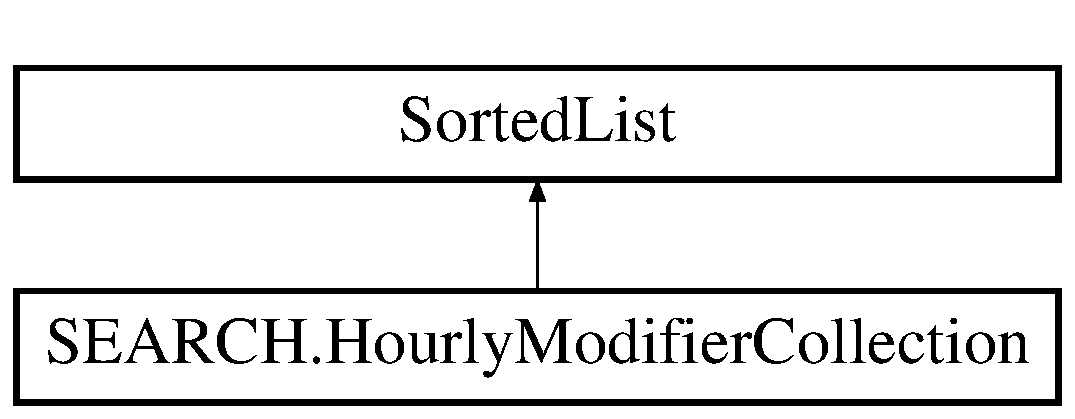
\includegraphics[height=2.000000cm]{class_s_e_a_r_c_h_1_1_hourly_modifier_collection}
\end{center}
\end{figure}
\subsection*{Public Member Functions}
\begin{DoxyCompactItemize}
\item 
\hyperlink{class_s_e_a_r_c_h_1_1_hourly_modifier}{Hourly\-Modifier} \hyperlink{class_s_e_a_r_c_h_1_1_hourly_modifier_collection_a51653c14e4d2f9a12f8eb252a93e5f09}{get\-Next} ()
\item 
void \hyperlink{class_s_e_a_r_c_h_1_1_hourly_modifier_collection_a3930bf2ae52037842365f412ddadec27}{reset} ()
\end{DoxyCompactItemize}
\subsection*{Static Public Member Functions}
\begin{DoxyCompactItemize}
\item 
static \hyperlink{class_s_e_a_r_c_h_1_1_hourly_modifier_collection}{Hourly\-Modifier\-Collection} \hyperlink{class_s_e_a_r_c_h_1_1_hourly_modifier_collection_a0454748be6b9c7508e81c16fa0db4c59}{Get\-Unique\-Instance} ()
\end{DoxyCompactItemize}
\subsection*{Properties}
\begin{DoxyCompactItemize}
\item 
int \hyperlink{class_s_e_a_r_c_h_1_1_hourly_modifier_collection_a6833cba60a501f4c5e22fd78636c6ade}{Next\-Start\-Hour}\hspace{0.3cm}{\ttfamily  \mbox{[}get, set\mbox{]}}
\end{DoxyCompactItemize}


\subsection{Member Function Documentation}
\hypertarget{class_s_e_a_r_c_h_1_1_hourly_modifier_collection_a51653c14e4d2f9a12f8eb252a93e5f09}{\index{S\-E\-A\-R\-C\-H\-::\-Hourly\-Modifier\-Collection@{S\-E\-A\-R\-C\-H\-::\-Hourly\-Modifier\-Collection}!get\-Next@{get\-Next}}
\index{get\-Next@{get\-Next}!SEARCH::HourlyModifierCollection@{S\-E\-A\-R\-C\-H\-::\-Hourly\-Modifier\-Collection}}
\subsubsection[{get\-Next}]{\setlength{\rightskip}{0pt plus 5cm}{\bf Hourly\-Modifier} S\-E\-A\-R\-C\-H.\-Hourly\-Modifier\-Collection.\-get\-Next (
\begin{DoxyParamCaption}
{}
\end{DoxyParamCaption}
)}}\label{class_s_e_a_r_c_h_1_1_hourly_modifier_collection_a51653c14e4d2f9a12f8eb252a93e5f09}
\hypertarget{class_s_e_a_r_c_h_1_1_hourly_modifier_collection_a0454748be6b9c7508e81c16fa0db4c59}{\index{S\-E\-A\-R\-C\-H\-::\-Hourly\-Modifier\-Collection@{S\-E\-A\-R\-C\-H\-::\-Hourly\-Modifier\-Collection}!Get\-Unique\-Instance@{Get\-Unique\-Instance}}
\index{Get\-Unique\-Instance@{Get\-Unique\-Instance}!SEARCH::HourlyModifierCollection@{S\-E\-A\-R\-C\-H\-::\-Hourly\-Modifier\-Collection}}
\subsubsection[{Get\-Unique\-Instance}]{\setlength{\rightskip}{0pt plus 5cm}static {\bf Hourly\-Modifier\-Collection} S\-E\-A\-R\-C\-H.\-Hourly\-Modifier\-Collection.\-Get\-Unique\-Instance (
\begin{DoxyParamCaption}
{}
\end{DoxyParamCaption}
)\hspace{0.3cm}{\ttfamily [static]}}}\label{class_s_e_a_r_c_h_1_1_hourly_modifier_collection_a0454748be6b9c7508e81c16fa0db4c59}
\hypertarget{class_s_e_a_r_c_h_1_1_hourly_modifier_collection_a3930bf2ae52037842365f412ddadec27}{\index{S\-E\-A\-R\-C\-H\-::\-Hourly\-Modifier\-Collection@{S\-E\-A\-R\-C\-H\-::\-Hourly\-Modifier\-Collection}!reset@{reset}}
\index{reset@{reset}!SEARCH::HourlyModifierCollection@{S\-E\-A\-R\-C\-H\-::\-Hourly\-Modifier\-Collection}}
\subsubsection[{reset}]{\setlength{\rightskip}{0pt plus 5cm}void S\-E\-A\-R\-C\-H.\-Hourly\-Modifier\-Collection.\-reset (
\begin{DoxyParamCaption}
{}
\end{DoxyParamCaption}
)}}\label{class_s_e_a_r_c_h_1_1_hourly_modifier_collection_a3930bf2ae52037842365f412ddadec27}


\subsection{Property Documentation}
\hypertarget{class_s_e_a_r_c_h_1_1_hourly_modifier_collection_a6833cba60a501f4c5e22fd78636c6ade}{\index{S\-E\-A\-R\-C\-H\-::\-Hourly\-Modifier\-Collection@{S\-E\-A\-R\-C\-H\-::\-Hourly\-Modifier\-Collection}!Next\-Start\-Hour@{Next\-Start\-Hour}}
\index{Next\-Start\-Hour@{Next\-Start\-Hour}!SEARCH::HourlyModifierCollection@{S\-E\-A\-R\-C\-H\-::\-Hourly\-Modifier\-Collection}}
\subsubsection[{Next\-Start\-Hour}]{\setlength{\rightskip}{0pt plus 5cm}int S\-E\-A\-R\-C\-H.\-Hourly\-Modifier\-Collection.\-Next\-Start\-Hour\hspace{0.3cm}{\ttfamily [get]}, {\ttfamily [set]}}}\label{class_s_e_a_r_c_h_1_1_hourly_modifier_collection_a6833cba60a501f4c5e22fd78636c6ade}


The documentation for this class was generated from the following file\-:\begin{DoxyCompactItemize}
\item 
Desktop/vlog4net\-A\-R\-C10\-\_\-64\-\_\-newhoming/\-Data\-Centric/\hyperlink{_hourly_modifier_collection_8cs}{Hourly\-Modifier\-Collection.\-cs}\end{DoxyCompactItemize}

\hypertarget{interface_s_e_a_r_c_h_1_1_i_attribute_observer}{\section{S\-E\-A\-R\-C\-H.\-I\-Attribute\-Observer Interface Reference}
\label{interface_s_e_a_r_c_h_1_1_i_attribute_observer}\index{S\-E\-A\-R\-C\-H.\-I\-Attribute\-Observer@{S\-E\-A\-R\-C\-H.\-I\-Attribute\-Observer}}
}


This interface defines the update method used to participate in the observer pattern  


\subsection*{Public Member Functions}
\begin{DoxyCompactItemize}
\item 
void \hyperlink{interface_s_e_a_r_c_h_1_1_i_attribute_observer_a74f7a537be7f58b889499eecd581cd0a}{update} (object new\-Value, object old\-Value)
\begin{DoxyCompactList}\small\item\em This method gets called by the attribute being observed. It is used by the observer to update whatever needs updating when the observed attribute changes. \end{DoxyCompactList}\end{DoxyCompactItemize}


\subsection{Detailed Description}
This interface defines the update method used to participate in the observer pattern 



\subsection{Member Function Documentation}
\hypertarget{interface_s_e_a_r_c_h_1_1_i_attribute_observer_a74f7a537be7f58b889499eecd581cd0a}{\index{S\-E\-A\-R\-C\-H\-::\-I\-Attribute\-Observer@{S\-E\-A\-R\-C\-H\-::\-I\-Attribute\-Observer}!update@{update}}
\index{update@{update}!SEARCH::IAttributeObserver@{S\-E\-A\-R\-C\-H\-::\-I\-Attribute\-Observer}}
\subsubsection[{update}]{\setlength{\rightskip}{0pt plus 5cm}void S\-E\-A\-R\-C\-H.\-I\-Attribute\-Observer.\-update (
\begin{DoxyParamCaption}
\item[{object}]{new\-Value, }
\item[{object}]{old\-Value}
\end{DoxyParamCaption}
)}}\label{interface_s_e_a_r_c_h_1_1_i_attribute_observer_a74f7a537be7f58b889499eecd581cd0a}


This method gets called by the attribute being observed. It is used by the observer to update whatever needs updating when the observed attribute changes. 



The documentation for this interface was generated from the following file\-:\begin{DoxyCompactItemize}
\item 
Desktop/vlog4net\-A\-R\-C10\-\_\-64\-\_\-newhoming/\-Data\-Centric/\hyperlink{_i_attribute_observer_8cs}{I\-Attribute\-Observer.\-cs}\end{DoxyCompactItemize}

\hypertarget{interface_s_e_a_r_c_h_1_1_i_home_range_criteria}{\section{S\-E\-A\-R\-C\-H.\-I\-Home\-Range\-Criteria Interface Reference}
\label{interface_s_e_a_r_c_h_1_1_i_home_range_criteria}\index{S\-E\-A\-R\-C\-H.\-I\-Home\-Range\-Criteria@{S\-E\-A\-R\-C\-H.\-I\-Home\-Range\-Criteria}}
}


Summary description for \hyperlink{interface_s_e_a_r_c_h_1_1_i_home_range_criteria}{I\-Home\-Range\-Criteria}.  


Inheritance diagram for S\-E\-A\-R\-C\-H.\-I\-Home\-Range\-Criteria\-:\begin{figure}[H]
\begin{center}
\leavevmode
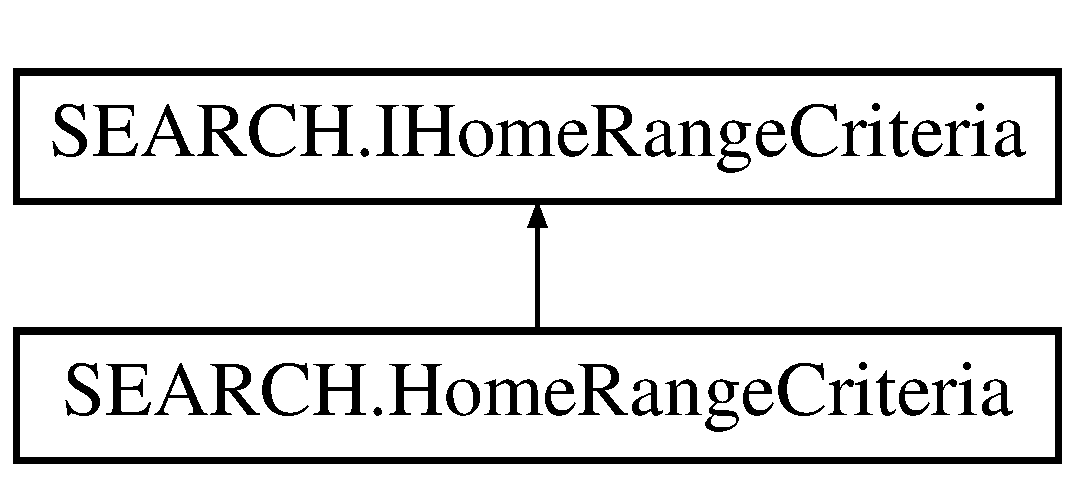
\includegraphics[height=2.000000cm]{interface_s_e_a_r_c_h_1_1_i_home_range_criteria}
\end{center}
\end{figure}
\subsection*{Properties}
\begin{DoxyCompactItemize}
\item 
double \hyperlink{interface_s_e_a_r_c_h_1_1_i_home_range_criteria_a9d4d6a0c16b83d50adaedc45aa4f679d}{Area}\hspace{0.3cm}{\ttfamily  \mbox{[}get, set\mbox{]}}
\item 
double \hyperlink{interface_s_e_a_r_c_h_1_1_i_home_range_criteria_a430d7f41fbeb75e48cf015fd44a27d6b}{Distance\-Mean}\hspace{0.3cm}{\ttfamily  \mbox{[}get, set\mbox{]}}
\item 
double \hyperlink{interface_s_e_a_r_c_h_1_1_i_home_range_criteria_a3a4572f0dcfd2b11d39d8a95ca1650b6}{Distance\-S\-D}\hspace{0.3cm}{\ttfamily  \mbox{[}get, set\mbox{]}}
\item 
double \hyperlink{interface_s_e_a_r_c_h_1_1_i_home_range_criteria_aaa1d0ebf77c4d646ba37afc36cce8299}{Distance\-Weight}\hspace{0.3cm}{\ttfamily  \mbox{[}get, set\mbox{]}}
\end{DoxyCompactItemize}


\subsection{Detailed Description}
Summary description for \hyperlink{interface_s_e_a_r_c_h_1_1_i_home_range_criteria}{I\-Home\-Range\-Criteria}. 



\subsection{Property Documentation}
\hypertarget{interface_s_e_a_r_c_h_1_1_i_home_range_criteria_a9d4d6a0c16b83d50adaedc45aa4f679d}{\index{S\-E\-A\-R\-C\-H\-::\-I\-Home\-Range\-Criteria@{S\-E\-A\-R\-C\-H\-::\-I\-Home\-Range\-Criteria}!Area@{Area}}
\index{Area@{Area}!SEARCH::IHomeRangeCriteria@{S\-E\-A\-R\-C\-H\-::\-I\-Home\-Range\-Criteria}}
\subsubsection[{Area}]{\setlength{\rightskip}{0pt plus 5cm}double S\-E\-A\-R\-C\-H.\-I\-Home\-Range\-Criteria.\-Area\hspace{0.3cm}{\ttfamily [get]}, {\ttfamily [set]}}}\label{interface_s_e_a_r_c_h_1_1_i_home_range_criteria_a9d4d6a0c16b83d50adaedc45aa4f679d}
\hypertarget{interface_s_e_a_r_c_h_1_1_i_home_range_criteria_a430d7f41fbeb75e48cf015fd44a27d6b}{\index{S\-E\-A\-R\-C\-H\-::\-I\-Home\-Range\-Criteria@{S\-E\-A\-R\-C\-H\-::\-I\-Home\-Range\-Criteria}!Distance\-Mean@{Distance\-Mean}}
\index{Distance\-Mean@{Distance\-Mean}!SEARCH::IHomeRangeCriteria@{S\-E\-A\-R\-C\-H\-::\-I\-Home\-Range\-Criteria}}
\subsubsection[{Distance\-Mean}]{\setlength{\rightskip}{0pt plus 5cm}double S\-E\-A\-R\-C\-H.\-I\-Home\-Range\-Criteria.\-Distance\-Mean\hspace{0.3cm}{\ttfamily [get]}, {\ttfamily [set]}}}\label{interface_s_e_a_r_c_h_1_1_i_home_range_criteria_a430d7f41fbeb75e48cf015fd44a27d6b}
\hypertarget{interface_s_e_a_r_c_h_1_1_i_home_range_criteria_a3a4572f0dcfd2b11d39d8a95ca1650b6}{\index{S\-E\-A\-R\-C\-H\-::\-I\-Home\-Range\-Criteria@{S\-E\-A\-R\-C\-H\-::\-I\-Home\-Range\-Criteria}!Distance\-S\-D@{Distance\-S\-D}}
\index{Distance\-S\-D@{Distance\-S\-D}!SEARCH::IHomeRangeCriteria@{S\-E\-A\-R\-C\-H\-::\-I\-Home\-Range\-Criteria}}
\subsubsection[{Distance\-S\-D}]{\setlength{\rightskip}{0pt plus 5cm}double S\-E\-A\-R\-C\-H.\-I\-Home\-Range\-Criteria.\-Distance\-S\-D\hspace{0.3cm}{\ttfamily [get]}, {\ttfamily [set]}}}\label{interface_s_e_a_r_c_h_1_1_i_home_range_criteria_a3a4572f0dcfd2b11d39d8a95ca1650b6}
\hypertarget{interface_s_e_a_r_c_h_1_1_i_home_range_criteria_aaa1d0ebf77c4d646ba37afc36cce8299}{\index{S\-E\-A\-R\-C\-H\-::\-I\-Home\-Range\-Criteria@{S\-E\-A\-R\-C\-H\-::\-I\-Home\-Range\-Criteria}!Distance\-Weight@{Distance\-Weight}}
\index{Distance\-Weight@{Distance\-Weight}!SEARCH::IHomeRangeCriteria@{S\-E\-A\-R\-C\-H\-::\-I\-Home\-Range\-Criteria}}
\subsubsection[{Distance\-Weight}]{\setlength{\rightskip}{0pt plus 5cm}double S\-E\-A\-R\-C\-H.\-I\-Home\-Range\-Criteria.\-Distance\-Weight\hspace{0.3cm}{\ttfamily [get]}, {\ttfamily [set]}}}\label{interface_s_e_a_r_c_h_1_1_i_home_range_criteria_aaa1d0ebf77c4d646ba37afc36cce8299}


The documentation for this interface was generated from the following file\-:\begin{DoxyCompactItemize}
\item 
Desktop/vlog4net\-A\-R\-C10\-\_\-64\-\_\-newhoming/\-Data\-Centric/\hyperlink{_i_home_range_criteria_8cs}{I\-Home\-Range\-Criteria.\-cs}\end{DoxyCompactItemize}

\hypertarget{interface_s_e_a_r_c_h_1_1_i_home_range_finder}{\section{S\-E\-A\-R\-C\-H.\-I\-Home\-Range\-Finder Interface Reference}
\label{interface_s_e_a_r_c_h_1_1_i_home_range_finder}\index{S\-E\-A\-R\-C\-H.\-I\-Home\-Range\-Finder@{S\-E\-A\-R\-C\-H.\-I\-Home\-Range\-Finder}}
}
Inheritance diagram for S\-E\-A\-R\-C\-H.\-I\-Home\-Range\-Finder\-:\begin{figure}[H]
\begin{center}
\leavevmode
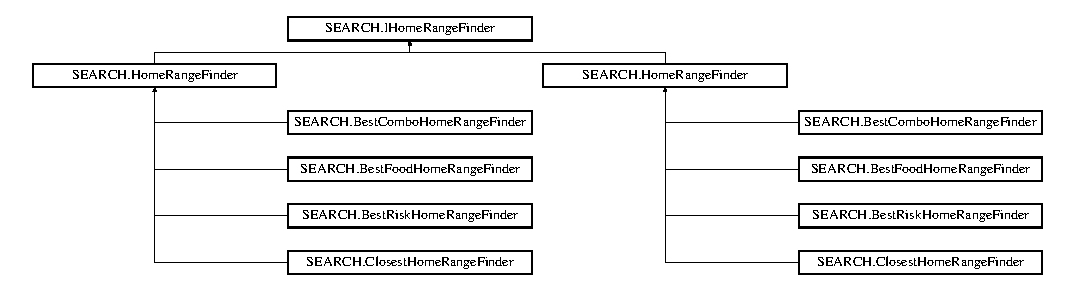
\includegraphics[height=3.456790cm]{interface_s_e_a_r_c_h_1_1_i_home_range_finder}
\end{center}
\end{figure}
\subsection*{Public Member Functions}
\begin{DoxyCompactItemize}
\item 
bool \hyperlink{interface_s_e_a_r_c_h_1_1_i_home_range_finder_aa22561856b66e114de8658a2b30bdb40}{set\-Home\-Range\-Center} (\hyperlink{class_s_e_a_r_c_h_1_1_animal}{Animal} in\-Animal, I\-Feature\-Class in\-Anmial\-Memory\-Map)
\item 
bool \hyperlink{interface_s_e_a_r_c_h_1_1_i_home_range_finder_a826e9e604bb2f25077d4896464f225a1}{set\-Home\-Range\-Center} (\hyperlink{class_s_e_a_r_c_h_1_1_animal}{Animal} in\-A, string in\-File\-Name)
\end{DoxyCompactItemize}


\subsection{Member Function Documentation}
\hypertarget{interface_s_e_a_r_c_h_1_1_i_home_range_finder_aa22561856b66e114de8658a2b30bdb40}{\index{S\-E\-A\-R\-C\-H\-::\-I\-Home\-Range\-Finder@{S\-E\-A\-R\-C\-H\-::\-I\-Home\-Range\-Finder}!set\-Home\-Range\-Center@{set\-Home\-Range\-Center}}
\index{set\-Home\-Range\-Center@{set\-Home\-Range\-Center}!SEARCH::IHomeRangeFinder@{S\-E\-A\-R\-C\-H\-::\-I\-Home\-Range\-Finder}}
\subsubsection[{set\-Home\-Range\-Center}]{\setlength{\rightskip}{0pt plus 5cm}bool S\-E\-A\-R\-C\-H.\-I\-Home\-Range\-Finder.\-set\-Home\-Range\-Center (
\begin{DoxyParamCaption}
\item[{{\bf Animal}}]{in\-Animal, }
\item[{I\-Feature\-Class}]{in\-Anmial\-Memory\-Map}
\end{DoxyParamCaption}
)}}\label{interface_s_e_a_r_c_h_1_1_i_home_range_finder_aa22561856b66e114de8658a2b30bdb40}
\hypertarget{interface_s_e_a_r_c_h_1_1_i_home_range_finder_a826e9e604bb2f25077d4896464f225a1}{\index{S\-E\-A\-R\-C\-H\-::\-I\-Home\-Range\-Finder@{S\-E\-A\-R\-C\-H\-::\-I\-Home\-Range\-Finder}!set\-Home\-Range\-Center@{set\-Home\-Range\-Center}}
\index{set\-Home\-Range\-Center@{set\-Home\-Range\-Center}!SEARCH::IHomeRangeFinder@{S\-E\-A\-R\-C\-H\-::\-I\-Home\-Range\-Finder}}
\subsubsection[{set\-Home\-Range\-Center}]{\setlength{\rightskip}{0pt plus 5cm}bool S\-E\-A\-R\-C\-H.\-I\-Home\-Range\-Finder.\-set\-Home\-Range\-Center (
\begin{DoxyParamCaption}
\item[{{\bf Animal}}]{in\-A, }
\item[{string}]{in\-File\-Name}
\end{DoxyParamCaption}
)}}\label{interface_s_e_a_r_c_h_1_1_i_home_range_finder_a826e9e604bb2f25077d4896464f225a1}


Implemented in \hyperlink{class_s_e_a_r_c_h_1_1_home_range_finder_a41b187329b1cd89b91c9c2f4a145ec7b}{S\-E\-A\-R\-C\-H.\-Home\-Range\-Finder}, \hyperlink{class_s_e_a_r_c_h_1_1_home_range_finder_a41b187329b1cd89b91c9c2f4a145ec7b}{S\-E\-A\-R\-C\-H.\-Home\-Range\-Finder}, \hyperlink{class_s_e_a_r_c_h_1_1_best_food_home_range_finder_aa9876f866a2bc8ffca635caafb20add3}{S\-E\-A\-R\-C\-H.\-Best\-Food\-Home\-Range\-Finder}, \hyperlink{class_s_e_a_r_c_h_1_1_best_combo_home_range_finder_a3ea0071e375fca09e9116bf627e205b5}{S\-E\-A\-R\-C\-H.\-Best\-Combo\-Home\-Range\-Finder}, \hyperlink{class_s_e_a_r_c_h_1_1_best_risk_home_range_finder_a90867156ad508254624d441fb9116d65}{S\-E\-A\-R\-C\-H.\-Best\-Risk\-Home\-Range\-Finder}, and \hyperlink{class_s_e_a_r_c_h_1_1_closest_home_range_finder_a9f4b1aae4a27e1109c03ea444fdaf185}{S\-E\-A\-R\-C\-H.\-Closest\-Home\-Range\-Finder}.



The documentation for this interface was generated from the following file\-:\begin{DoxyCompactItemize}
\item 
Desktop/vlog4net\-A\-R\-C10\-\_\-64\-\_\-newhoming/\-Data\-Centric/\hyperlink{_i_home_range_finder_8cs}{I\-Home\-Range\-Finder.\-cs}\end{DoxyCompactItemize}

\hypertarget{interface_s_e_a_r_c_h_1_1_i_home_range_trigger}{\section{S\-E\-A\-R\-C\-H.\-I\-Home\-Range\-Trigger Interface Reference}
\label{interface_s_e_a_r_c_h_1_1_i_home_range_trigger}\index{S\-E\-A\-R\-C\-H.\-I\-Home\-Range\-Trigger@{S\-E\-A\-R\-C\-H.\-I\-Home\-Range\-Trigger}}
}
Inheritance diagram for S\-E\-A\-R\-C\-H.\-I\-Home\-Range\-Trigger\-:\begin{figure}[H]
\begin{center}
\leavevmode
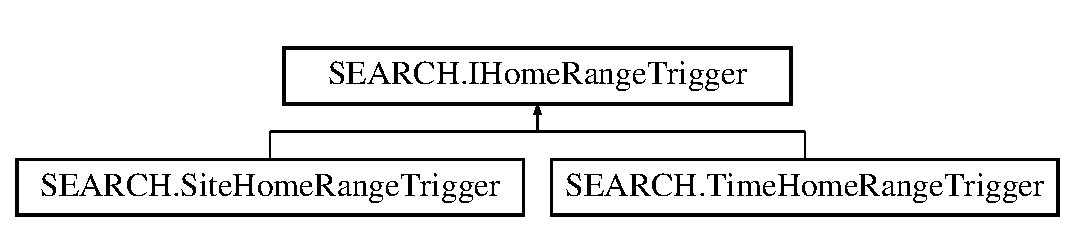
\includegraphics[height=2.000000cm]{interface_s_e_a_r_c_h_1_1_i_home_range_trigger}
\end{center}
\end{figure}
\subsection*{Public Member Functions}
\begin{DoxyCompactItemize}
\item 
bool \hyperlink{interface_s_e_a_r_c_h_1_1_i_home_range_trigger_ac7476deb63d55a92c635d2d4a479db4d}{time\-To\-Look\-For\-Home} (\hyperlink{class_s_e_a_r_c_h_1_1_animal}{Animal} in\-A)
\item 
void \hyperlink{interface_s_e_a_r_c_h_1_1_i_home_range_trigger_a3d6cabe1057278e2c4369649254baea6}{reset} (int num)
\end{DoxyCompactItemize}
\subsection*{Properties}
\begin{DoxyCompactItemize}
\item 
int \hyperlink{interface_s_e_a_r_c_h_1_1_i_home_range_trigger_a7cf9d69e497b24d178b17824586cbcbd}{num\-Times}\hspace{0.3cm}{\ttfamily  \mbox{[}get, set\mbox{]}}
\end{DoxyCompactItemize}


\subsection{Member Function Documentation}
\hypertarget{interface_s_e_a_r_c_h_1_1_i_home_range_trigger_a3d6cabe1057278e2c4369649254baea6}{\index{S\-E\-A\-R\-C\-H\-::\-I\-Home\-Range\-Trigger@{S\-E\-A\-R\-C\-H\-::\-I\-Home\-Range\-Trigger}!reset@{reset}}
\index{reset@{reset}!SEARCH::IHomeRangeTrigger@{S\-E\-A\-R\-C\-H\-::\-I\-Home\-Range\-Trigger}}
\subsubsection[{reset}]{\setlength{\rightskip}{0pt plus 5cm}void S\-E\-A\-R\-C\-H.\-I\-Home\-Range\-Trigger.\-reset (
\begin{DoxyParamCaption}
\item[{int}]{num}
\end{DoxyParamCaption}
)}}\label{interface_s_e_a_r_c_h_1_1_i_home_range_trigger_a3d6cabe1057278e2c4369649254baea6}


Implemented in \hyperlink{class_s_e_a_r_c_h_1_1_site_home_range_trigger_a7266d98080f93ce4ad13e0b6ecfa805c}{S\-E\-A\-R\-C\-H.\-Site\-Home\-Range\-Trigger}, and \hyperlink{class_s_e_a_r_c_h_1_1_time_home_range_trigger_afd1bace9c699ecf623e4ee72596873e4}{S\-E\-A\-R\-C\-H.\-Time\-Home\-Range\-Trigger}.

\hypertarget{interface_s_e_a_r_c_h_1_1_i_home_range_trigger_ac7476deb63d55a92c635d2d4a479db4d}{\index{S\-E\-A\-R\-C\-H\-::\-I\-Home\-Range\-Trigger@{S\-E\-A\-R\-C\-H\-::\-I\-Home\-Range\-Trigger}!time\-To\-Look\-For\-Home@{time\-To\-Look\-For\-Home}}
\index{time\-To\-Look\-For\-Home@{time\-To\-Look\-For\-Home}!SEARCH::IHomeRangeTrigger@{S\-E\-A\-R\-C\-H\-::\-I\-Home\-Range\-Trigger}}
\subsubsection[{time\-To\-Look\-For\-Home}]{\setlength{\rightskip}{0pt plus 5cm}bool S\-E\-A\-R\-C\-H.\-I\-Home\-Range\-Trigger.\-time\-To\-Look\-For\-Home (
\begin{DoxyParamCaption}
\item[{{\bf Animal}}]{in\-A}
\end{DoxyParamCaption}
)}}\label{interface_s_e_a_r_c_h_1_1_i_home_range_trigger_ac7476deb63d55a92c635d2d4a479db4d}


Implemented in \hyperlink{class_s_e_a_r_c_h_1_1_site_home_range_trigger_a89af0390fd4719b591b674c4f9f60863}{S\-E\-A\-R\-C\-H.\-Site\-Home\-Range\-Trigger}, and \hyperlink{class_s_e_a_r_c_h_1_1_time_home_range_trigger_ad480f427e0e81b0331efd1e393b3dd65}{S\-E\-A\-R\-C\-H.\-Time\-Home\-Range\-Trigger}.



\subsection{Property Documentation}
\hypertarget{interface_s_e_a_r_c_h_1_1_i_home_range_trigger_a7cf9d69e497b24d178b17824586cbcbd}{\index{S\-E\-A\-R\-C\-H\-::\-I\-Home\-Range\-Trigger@{S\-E\-A\-R\-C\-H\-::\-I\-Home\-Range\-Trigger}!num\-Times@{num\-Times}}
\index{num\-Times@{num\-Times}!SEARCH::IHomeRangeTrigger@{S\-E\-A\-R\-C\-H\-::\-I\-Home\-Range\-Trigger}}
\subsubsection[{num\-Times}]{\setlength{\rightskip}{0pt plus 5cm}int S\-E\-A\-R\-C\-H.\-I\-Home\-Range\-Trigger.\-num\-Times\hspace{0.3cm}{\ttfamily [get]}, {\ttfamily [set]}}}\label{interface_s_e_a_r_c_h_1_1_i_home_range_trigger_a7cf9d69e497b24d178b17824586cbcbd}


The documentation for this interface was generated from the following file\-:\begin{DoxyCompactItemize}
\item 
Desktop/vlog4net\-A\-R\-C10\-\_\-64\-\_\-newhoming/\-Data\-Centric/\hyperlink{_i_home_range_trigger_8cs}{I\-Home\-Range\-Trigger.\-cs}\end{DoxyCompactItemize}

\hypertarget{class_s_e_a_r_c_h_1_1_initial_animal_attributes}{\section{S\-E\-A\-R\-C\-H.\-Initial\-Animal\-Attributes Class Reference}
\label{class_s_e_a_r_c_h_1_1_initial_animal_attributes}\index{S\-E\-A\-R\-C\-H.\-Initial\-Animal\-Attributes@{S\-E\-A\-R\-C\-H.\-Initial\-Animal\-Attributes}}
}


Summary description for \hyperlink{class_s_e_a_r_c_h_1_1_initial_animal_attributes}{Initial\-Animal\-Attributes}.  


\subsection*{Public Member Functions}
\begin{DoxyCompactItemize}
\item 
\hyperlink{class_s_e_a_r_c_h_1_1_initial_animal_attributes_a525bf4ba782d522d1bea36d53e59a004}{Initial\-Animal\-Attributes} ()
\item 
void \hyperlink{class_s_e_a_r_c_h_1_1_initial_animal_attributes_abd1c34d82c605d328dc45d12ae9189c9}{set\-Point\-Values} (I\-Point in\-P)
\end{DoxyCompactItemize}
\subsection*{Properties}
\begin{DoxyCompactItemize}
\item 
string \hyperlink{class_s_e_a_r_c_h_1_1_initial_animal_attributes_a657b581df7f956dd0d71f859896bb75e}{Orginal\-I\-D}\hspace{0.3cm}{\ttfamily  \mbox{[}get, set\mbox{]}}
\item 
char \hyperlink{class_s_e_a_r_c_h_1_1_initial_animal_attributes_aacb87a569062245a6f75e83ff1eee1d1}{Sex}\hspace{0.3cm}{\ttfamily  \mbox{[}get, set\mbox{]}}
\item 
I\-Point \hyperlink{class_s_e_a_r_c_h_1_1_initial_animal_attributes_a855323a46a243ea936451da3d04fa0a7}{Location}\hspace{0.3cm}{\ttfamily  \mbox{[}get, set\mbox{]}}
\item 
int \hyperlink{class_s_e_a_r_c_h_1_1_initial_animal_attributes_ab5edf1fff77568b74fe69b83a283dcf2}{Num\-To\-Make}\hspace{0.3cm}{\ttfamily  \mbox{[}get, set\mbox{]}}
\end{DoxyCompactItemize}


\subsection{Detailed Description}
Summary description for \hyperlink{class_s_e_a_r_c_h_1_1_initial_animal_attributes}{Initial\-Animal\-Attributes}. 



\subsection{Constructor \& Destructor Documentation}
\hypertarget{class_s_e_a_r_c_h_1_1_initial_animal_attributes_a525bf4ba782d522d1bea36d53e59a004}{\index{S\-E\-A\-R\-C\-H\-::\-Initial\-Animal\-Attributes@{S\-E\-A\-R\-C\-H\-::\-Initial\-Animal\-Attributes}!Initial\-Animal\-Attributes@{Initial\-Animal\-Attributes}}
\index{Initial\-Animal\-Attributes@{Initial\-Animal\-Attributes}!SEARCH::InitialAnimalAttributes@{S\-E\-A\-R\-C\-H\-::\-Initial\-Animal\-Attributes}}
\subsubsection[{Initial\-Animal\-Attributes}]{\setlength{\rightskip}{0pt plus 5cm}S\-E\-A\-R\-C\-H.\-Initial\-Animal\-Attributes.\-Initial\-Animal\-Attributes (
\begin{DoxyParamCaption}
{}
\end{DoxyParamCaption}
)}}\label{class_s_e_a_r_c_h_1_1_initial_animal_attributes_a525bf4ba782d522d1bea36d53e59a004}


\subsection{Member Function Documentation}
\hypertarget{class_s_e_a_r_c_h_1_1_initial_animal_attributes_abd1c34d82c605d328dc45d12ae9189c9}{\index{S\-E\-A\-R\-C\-H\-::\-Initial\-Animal\-Attributes@{S\-E\-A\-R\-C\-H\-::\-Initial\-Animal\-Attributes}!set\-Point\-Values@{set\-Point\-Values}}
\index{set\-Point\-Values@{set\-Point\-Values}!SEARCH::InitialAnimalAttributes@{S\-E\-A\-R\-C\-H\-::\-Initial\-Animal\-Attributes}}
\subsubsection[{set\-Point\-Values}]{\setlength{\rightskip}{0pt plus 5cm}void S\-E\-A\-R\-C\-H.\-Initial\-Animal\-Attributes.\-set\-Point\-Values (
\begin{DoxyParamCaption}
\item[{I\-Point}]{in\-P}
\end{DoxyParamCaption}
)}}\label{class_s_e_a_r_c_h_1_1_initial_animal_attributes_abd1c34d82c605d328dc45d12ae9189c9}


\subsection{Property Documentation}
\hypertarget{class_s_e_a_r_c_h_1_1_initial_animal_attributes_a855323a46a243ea936451da3d04fa0a7}{\index{S\-E\-A\-R\-C\-H\-::\-Initial\-Animal\-Attributes@{S\-E\-A\-R\-C\-H\-::\-Initial\-Animal\-Attributes}!Location@{Location}}
\index{Location@{Location}!SEARCH::InitialAnimalAttributes@{S\-E\-A\-R\-C\-H\-::\-Initial\-Animal\-Attributes}}
\subsubsection[{Location}]{\setlength{\rightskip}{0pt plus 5cm}I\-Point S\-E\-A\-R\-C\-H.\-Initial\-Animal\-Attributes.\-Location\hspace{0.3cm}{\ttfamily [get]}, {\ttfamily [set]}}}\label{class_s_e_a_r_c_h_1_1_initial_animal_attributes_a855323a46a243ea936451da3d04fa0a7}
\hypertarget{class_s_e_a_r_c_h_1_1_initial_animal_attributes_ab5edf1fff77568b74fe69b83a283dcf2}{\index{S\-E\-A\-R\-C\-H\-::\-Initial\-Animal\-Attributes@{S\-E\-A\-R\-C\-H\-::\-Initial\-Animal\-Attributes}!Num\-To\-Make@{Num\-To\-Make}}
\index{Num\-To\-Make@{Num\-To\-Make}!SEARCH::InitialAnimalAttributes@{S\-E\-A\-R\-C\-H\-::\-Initial\-Animal\-Attributes}}
\subsubsection[{Num\-To\-Make}]{\setlength{\rightskip}{0pt plus 5cm}int S\-E\-A\-R\-C\-H.\-Initial\-Animal\-Attributes.\-Num\-To\-Make\hspace{0.3cm}{\ttfamily [get]}, {\ttfamily [set]}}}\label{class_s_e_a_r_c_h_1_1_initial_animal_attributes_ab5edf1fff77568b74fe69b83a283dcf2}
\hypertarget{class_s_e_a_r_c_h_1_1_initial_animal_attributes_a657b581df7f956dd0d71f859896bb75e}{\index{S\-E\-A\-R\-C\-H\-::\-Initial\-Animal\-Attributes@{S\-E\-A\-R\-C\-H\-::\-Initial\-Animal\-Attributes}!Orginal\-I\-D@{Orginal\-I\-D}}
\index{Orginal\-I\-D@{Orginal\-I\-D}!SEARCH::InitialAnimalAttributes@{S\-E\-A\-R\-C\-H\-::\-Initial\-Animal\-Attributes}}
\subsubsection[{Orginal\-I\-D}]{\setlength{\rightskip}{0pt plus 5cm}string S\-E\-A\-R\-C\-H.\-Initial\-Animal\-Attributes.\-Orginal\-I\-D\hspace{0.3cm}{\ttfamily [get]}, {\ttfamily [set]}}}\label{class_s_e_a_r_c_h_1_1_initial_animal_attributes_a657b581df7f956dd0d71f859896bb75e}
\hypertarget{class_s_e_a_r_c_h_1_1_initial_animal_attributes_aacb87a569062245a6f75e83ff1eee1d1}{\index{S\-E\-A\-R\-C\-H\-::\-Initial\-Animal\-Attributes@{S\-E\-A\-R\-C\-H\-::\-Initial\-Animal\-Attributes}!Sex@{Sex}}
\index{Sex@{Sex}!SEARCH::InitialAnimalAttributes@{S\-E\-A\-R\-C\-H\-::\-Initial\-Animal\-Attributes}}
\subsubsection[{Sex}]{\setlength{\rightskip}{0pt plus 5cm}char S\-E\-A\-R\-C\-H.\-Initial\-Animal\-Attributes.\-Sex\hspace{0.3cm}{\ttfamily [get]}, {\ttfamily [set]}}}\label{class_s_e_a_r_c_h_1_1_initial_animal_attributes_aacb87a569062245a6f75e83ff1eee1d1}


The documentation for this class was generated from the following file\-:\begin{DoxyCompactItemize}
\item 
Desktop/vlog4net\-A\-R\-C10\-\_\-64\-\_\-newhoming/\-Data\-Centric/\hyperlink{_initial_animal_attributes_8cs}{Initial\-Animal\-Attributes.\-cs}\end{DoxyCompactItemize}

\hypertarget{class_s_e_a_r_c_h_1_1_initial_resident_info}{\section{S\-E\-A\-R\-C\-H.\-Initial\-Resident\-Info Class Reference}
\label{class_s_e_a_r_c_h_1_1_initial_resident_info}\index{S\-E\-A\-R\-C\-H.\-Initial\-Resident\-Info@{S\-E\-A\-R\-C\-H.\-Initial\-Resident\-Info}}
}


Summary description for \hyperlink{class_s_e_a_r_c_h_1_1_initial_resident_info}{Initial\-Resident\-Info}.  


\subsection*{Public Member Functions}
\begin{DoxyCompactItemize}
\item 
\hyperlink{class_s_e_a_r_c_h_1_1_initial_resident_info_a4a02216bc1d8b3e6cc728cc7c0037a48}{Initial\-Resident\-Info} ()
\end{DoxyCompactItemize}
\subsection*{Properties}
\begin{DoxyCompactItemize}
\item 
I\-Point \hyperlink{class_s_e_a_r_c_h_1_1_initial_resident_info_a9d0dd0f308b66c00fdd38827085e581b}{Location}\hspace{0.3cm}{\ttfamily  \mbox{[}get, set\mbox{]}}
\item 
string \hyperlink{class_s_e_a_r_c_h_1_1_initial_resident_info_ade021018937f83c61e36e6bccc15d485}{Sex}\hspace{0.3cm}{\ttfamily  \mbox{[}get, set\mbox{]}}
\end{DoxyCompactItemize}


\subsection{Detailed Description}
Summary description for \hyperlink{class_s_e_a_r_c_h_1_1_initial_resident_info}{Initial\-Resident\-Info}. 



\subsection{Constructor \& Destructor Documentation}
\hypertarget{class_s_e_a_r_c_h_1_1_initial_resident_info_a4a02216bc1d8b3e6cc728cc7c0037a48}{\index{S\-E\-A\-R\-C\-H\-::\-Initial\-Resident\-Info@{S\-E\-A\-R\-C\-H\-::\-Initial\-Resident\-Info}!Initial\-Resident\-Info@{Initial\-Resident\-Info}}
\index{Initial\-Resident\-Info@{Initial\-Resident\-Info}!SEARCH::InitialResidentInfo@{S\-E\-A\-R\-C\-H\-::\-Initial\-Resident\-Info}}
\subsubsection[{Initial\-Resident\-Info}]{\setlength{\rightskip}{0pt plus 5cm}S\-E\-A\-R\-C\-H.\-Initial\-Resident\-Info.\-Initial\-Resident\-Info (
\begin{DoxyParamCaption}
{}
\end{DoxyParamCaption}
)}}\label{class_s_e_a_r_c_h_1_1_initial_resident_info_a4a02216bc1d8b3e6cc728cc7c0037a48}


\subsection{Property Documentation}
\hypertarget{class_s_e_a_r_c_h_1_1_initial_resident_info_a9d0dd0f308b66c00fdd38827085e581b}{\index{S\-E\-A\-R\-C\-H\-::\-Initial\-Resident\-Info@{S\-E\-A\-R\-C\-H\-::\-Initial\-Resident\-Info}!Location@{Location}}
\index{Location@{Location}!SEARCH::InitialResidentInfo@{S\-E\-A\-R\-C\-H\-::\-Initial\-Resident\-Info}}
\subsubsection[{Location}]{\setlength{\rightskip}{0pt plus 5cm}I\-Point S\-E\-A\-R\-C\-H.\-Initial\-Resident\-Info.\-Location\hspace{0.3cm}{\ttfamily [get]}, {\ttfamily [set]}}}\label{class_s_e_a_r_c_h_1_1_initial_resident_info_a9d0dd0f308b66c00fdd38827085e581b}
\hypertarget{class_s_e_a_r_c_h_1_1_initial_resident_info_ade021018937f83c61e36e6bccc15d485}{\index{S\-E\-A\-R\-C\-H\-::\-Initial\-Resident\-Info@{S\-E\-A\-R\-C\-H\-::\-Initial\-Resident\-Info}!Sex@{Sex}}
\index{Sex@{Sex}!SEARCH::InitialResidentInfo@{S\-E\-A\-R\-C\-H\-::\-Initial\-Resident\-Info}}
\subsubsection[{Sex}]{\setlength{\rightskip}{0pt plus 5cm}string S\-E\-A\-R\-C\-H.\-Initial\-Resident\-Info.\-Sex\hspace{0.3cm}{\ttfamily [get]}, {\ttfamily [set]}}}\label{class_s_e_a_r_c_h_1_1_initial_resident_info_ade021018937f83c61e36e6bccc15d485}


The documentation for this class was generated from the following file\-:\begin{DoxyCompactItemize}
\item 
Desktop/vlog4net\-A\-R\-C10\-\_\-64\-\_\-newhoming/\-Data\-Centric/\hyperlink{_initial_resident_info_8cs}{Initial\-Resident\-Info.\-cs}\end{DoxyCompactItemize}

\hypertarget{class_s_e_a_r_c_h_1_1_i_point_list}{\section{S\-E\-A\-R\-C\-H.\-I\-Point\-List Class Reference}
\label{class_s_e_a_r_c_h_1_1_i_point_list}\index{S\-E\-A\-R\-C\-H.\-I\-Point\-List@{S\-E\-A\-R\-C\-H.\-I\-Point\-List}}
}


Summary description for \hyperlink{class_s_e_a_r_c_h_1_1_i_point_list}{I\-Point\-List}.  


\subsection*{Public Member Functions}
\begin{DoxyCompactItemize}
\item 
\hyperlink{class_s_e_a_r_c_h_1_1_i_point_list_a3af15b08aac6355d650f3258cde0d88b}{I\-Point\-List} ()
\item 
void \hyperlink{class_s_e_a_r_c_h_1_1_i_point_list_af71c94382995f0c502e4534375619535}{add} (I\-Point in\-Point)
\item 
int \hyperlink{class_s_e_a_r_c_h_1_1_i_point_list_a5e843c9280b68b78b887c7b824a5279b}{Count} ()
\item 
int \hyperlink{class_s_e_a_r_c_h_1_1_i_point_list_a43d755ce04da0e154b8a58344b2c5860}{get\-Last\-Index} ()
\item 
I\-Point \hyperlink{class_s_e_a_r_c_h_1_1_i_point_list_ab04c40a619d61c9ad1b90c7e0e9622ac}{get\-Point\-By\-Index} (int i)
\end{DoxyCompactItemize}
\subsection*{Properties}
\begin{DoxyCompactItemize}
\item 
I\-Point \hyperlink{class_s_e_a_r_c_h_1_1_i_point_list_a558dbec58b22e46745973e7136ac1ea3}{this\mbox{[}int i\mbox{]}}\hspace{0.3cm}{\ttfamily  \mbox{[}get, set\mbox{]}}
\end{DoxyCompactItemize}


\subsection{Detailed Description}
Summary description for \hyperlink{class_s_e_a_r_c_h_1_1_i_point_list}{I\-Point\-List}. 



\subsection{Constructor \& Destructor Documentation}
\hypertarget{class_s_e_a_r_c_h_1_1_i_point_list_a3af15b08aac6355d650f3258cde0d88b}{\index{S\-E\-A\-R\-C\-H\-::\-I\-Point\-List@{S\-E\-A\-R\-C\-H\-::\-I\-Point\-List}!I\-Point\-List@{I\-Point\-List}}
\index{I\-Point\-List@{I\-Point\-List}!SEARCH::IPointList@{S\-E\-A\-R\-C\-H\-::\-I\-Point\-List}}
\subsubsection[{I\-Point\-List}]{\setlength{\rightskip}{0pt plus 5cm}S\-E\-A\-R\-C\-H.\-I\-Point\-List.\-I\-Point\-List (
\begin{DoxyParamCaption}
{}
\end{DoxyParamCaption}
)}}\label{class_s_e_a_r_c_h_1_1_i_point_list_a3af15b08aac6355d650f3258cde0d88b}


\subsection{Member Function Documentation}
\hypertarget{class_s_e_a_r_c_h_1_1_i_point_list_af71c94382995f0c502e4534375619535}{\index{S\-E\-A\-R\-C\-H\-::\-I\-Point\-List@{S\-E\-A\-R\-C\-H\-::\-I\-Point\-List}!add@{add}}
\index{add@{add}!SEARCH::IPointList@{S\-E\-A\-R\-C\-H\-::\-I\-Point\-List}}
\subsubsection[{add}]{\setlength{\rightskip}{0pt plus 5cm}void S\-E\-A\-R\-C\-H.\-I\-Point\-List.\-add (
\begin{DoxyParamCaption}
\item[{I\-Point}]{in\-Point}
\end{DoxyParamCaption}
)}}\label{class_s_e_a_r_c_h_1_1_i_point_list_af71c94382995f0c502e4534375619535}
\hypertarget{class_s_e_a_r_c_h_1_1_i_point_list_a5e843c9280b68b78b887c7b824a5279b}{\index{S\-E\-A\-R\-C\-H\-::\-I\-Point\-List@{S\-E\-A\-R\-C\-H\-::\-I\-Point\-List}!Count@{Count}}
\index{Count@{Count}!SEARCH::IPointList@{S\-E\-A\-R\-C\-H\-::\-I\-Point\-List}}
\subsubsection[{Count}]{\setlength{\rightskip}{0pt plus 5cm}int S\-E\-A\-R\-C\-H.\-I\-Point\-List.\-Count (
\begin{DoxyParamCaption}
{}
\end{DoxyParamCaption}
)}}\label{class_s_e_a_r_c_h_1_1_i_point_list_a5e843c9280b68b78b887c7b824a5279b}
\hypertarget{class_s_e_a_r_c_h_1_1_i_point_list_a43d755ce04da0e154b8a58344b2c5860}{\index{S\-E\-A\-R\-C\-H\-::\-I\-Point\-List@{S\-E\-A\-R\-C\-H\-::\-I\-Point\-List}!get\-Last\-Index@{get\-Last\-Index}}
\index{get\-Last\-Index@{get\-Last\-Index}!SEARCH::IPointList@{S\-E\-A\-R\-C\-H\-::\-I\-Point\-List}}
\subsubsection[{get\-Last\-Index}]{\setlength{\rightskip}{0pt plus 5cm}int S\-E\-A\-R\-C\-H.\-I\-Point\-List.\-get\-Last\-Index (
\begin{DoxyParamCaption}
{}
\end{DoxyParamCaption}
)}}\label{class_s_e_a_r_c_h_1_1_i_point_list_a43d755ce04da0e154b8a58344b2c5860}
\hypertarget{class_s_e_a_r_c_h_1_1_i_point_list_ab04c40a619d61c9ad1b90c7e0e9622ac}{\index{S\-E\-A\-R\-C\-H\-::\-I\-Point\-List@{S\-E\-A\-R\-C\-H\-::\-I\-Point\-List}!get\-Point\-By\-Index@{get\-Point\-By\-Index}}
\index{get\-Point\-By\-Index@{get\-Point\-By\-Index}!SEARCH::IPointList@{S\-E\-A\-R\-C\-H\-::\-I\-Point\-List}}
\subsubsection[{get\-Point\-By\-Index}]{\setlength{\rightskip}{0pt plus 5cm}I\-Point S\-E\-A\-R\-C\-H.\-I\-Point\-List.\-get\-Point\-By\-Index (
\begin{DoxyParamCaption}
\item[{int}]{i}
\end{DoxyParamCaption}
)}}\label{class_s_e_a_r_c_h_1_1_i_point_list_ab04c40a619d61c9ad1b90c7e0e9622ac}


\subsection{Property Documentation}
\hypertarget{class_s_e_a_r_c_h_1_1_i_point_list_a558dbec58b22e46745973e7136ac1ea3}{\index{S\-E\-A\-R\-C\-H\-::\-I\-Point\-List@{S\-E\-A\-R\-C\-H\-::\-I\-Point\-List}!this\mbox{[}int i\mbox{]}@{this[int i]}}
\index{this\mbox{[}int i\mbox{]}@{this[int i]}!SEARCH::IPointList@{S\-E\-A\-R\-C\-H\-::\-I\-Point\-List}}
\subsubsection[{this[int i]}]{\setlength{\rightskip}{0pt plus 5cm}I\-Point S\-E\-A\-R\-C\-H.\-I\-Point\-List.\-this\mbox{[}int i\mbox{]}\hspace{0.3cm}{\ttfamily [get]}, {\ttfamily [set]}}}\label{class_s_e_a_r_c_h_1_1_i_point_list_a558dbec58b22e46745973e7136ac1ea3}


The documentation for this class was generated from the following file\-:\begin{DoxyCompactItemize}
\item 
Desktop/vlog4net\-A\-R\-C10\-\_\-64\-\_\-newhoming/\-Data\-Centric/\hyperlink{_i_point_list_8cs}{I\-Point\-List.\-cs}\end{DoxyCompactItemize}

\hypertarget{class_s_e_a_r_c_h_1_1_male}{\section{S\-E\-A\-R\-C\-H.\-Male Class Reference}
\label{class_s_e_a_r_c_h_1_1_male}\index{S\-E\-A\-R\-C\-H.\-Male@{S\-E\-A\-R\-C\-H.\-Male}}
}
Inheritance diagram for S\-E\-A\-R\-C\-H.\-Male\-:\begin{figure}[H]
\begin{center}
\leavevmode
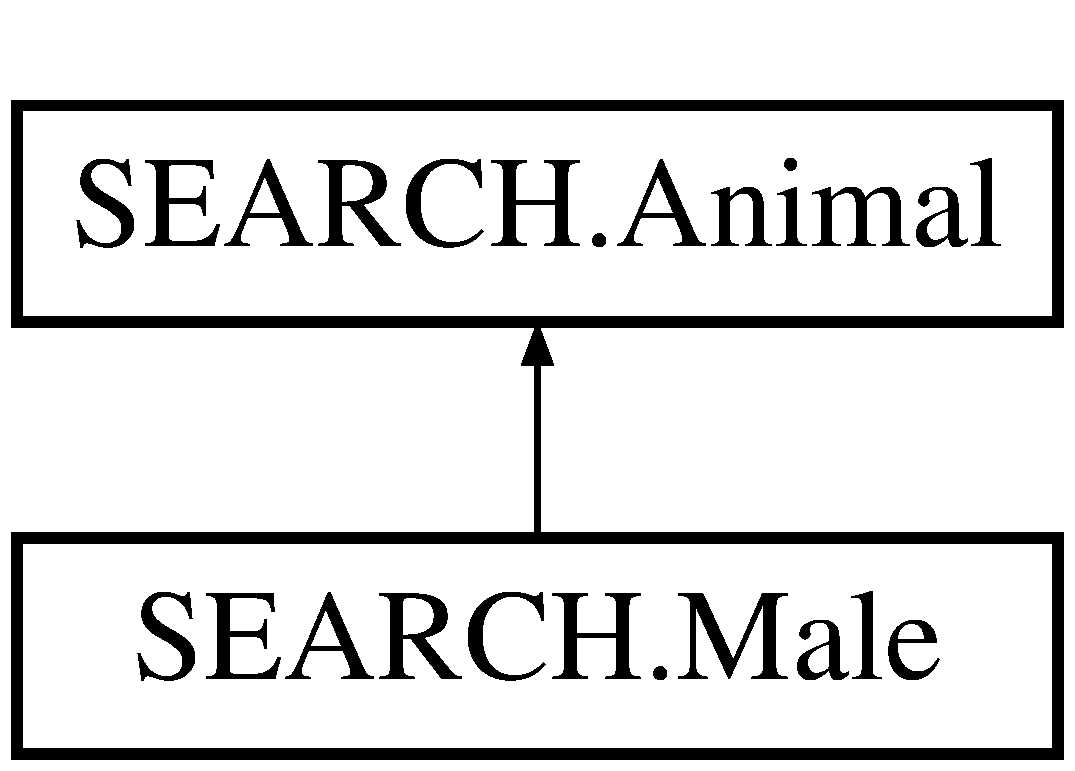
\includegraphics[height=2.000000cm]{class_s_e_a_r_c_h_1_1_male}
\end{center}
\end{figure}
\subsection*{Public Member Functions}
\begin{DoxyCompactItemize}
\item 
\hyperlink{class_s_e_a_r_c_h_1_1_male_af34edc865c9711c5ac8caf975ce0b08a}{Male} ()
\item 
override void \hyperlink{class_s_e_a_r_c_h_1_1_male_ae2c3be6f7a6daf01e72f2a7c6af0007e}{dump} ()
\end{DoxyCompactItemize}
\subsection*{Additional Inherited Members}


\subsection{Constructor \& Destructor Documentation}
\hypertarget{class_s_e_a_r_c_h_1_1_male_af34edc865c9711c5ac8caf975ce0b08a}{\index{S\-E\-A\-R\-C\-H\-::\-Male@{S\-E\-A\-R\-C\-H\-::\-Male}!Male@{Male}}
\index{Male@{Male}!SEARCH::Male@{S\-E\-A\-R\-C\-H\-::\-Male}}
\subsubsection[{Male}]{\setlength{\rightskip}{0pt plus 5cm}S\-E\-A\-R\-C\-H.\-Male.\-Male (
\begin{DoxyParamCaption}
{}
\end{DoxyParamCaption}
)}}\label{class_s_e_a_r_c_h_1_1_male_af34edc865c9711c5ac8caf975ce0b08a}


\subsection{Member Function Documentation}
\hypertarget{class_s_e_a_r_c_h_1_1_male_ae2c3be6f7a6daf01e72f2a7c6af0007e}{\index{S\-E\-A\-R\-C\-H\-::\-Male@{S\-E\-A\-R\-C\-H\-::\-Male}!dump@{dump}}
\index{dump@{dump}!SEARCH::Male@{S\-E\-A\-R\-C\-H\-::\-Male}}
\subsubsection[{dump}]{\setlength{\rightskip}{0pt plus 5cm}override void S\-E\-A\-R\-C\-H.\-Male.\-dump (
\begin{DoxyParamCaption}
{}
\end{DoxyParamCaption}
)\hspace{0.3cm}{\ttfamily [virtual]}}}\label{class_s_e_a_r_c_h_1_1_male_ae2c3be6f7a6daf01e72f2a7c6af0007e}


Reimplemented from \hyperlink{class_s_e_a_r_c_h_1_1_animal_ade2aab75e98f185a6f9ab2a5a9244bd3}{S\-E\-A\-R\-C\-H.\-Animal}.



The documentation for this class was generated from the following file\-:\begin{DoxyCompactItemize}
\item 
Desktop/vlog4net\-A\-R\-C10\-\_\-64\-\_\-newhoming/\-Data\-Centric/\hyperlink{_male_animal_8cs}{Male\-Animal.\-cs}\end{DoxyCompactItemize}

\hypertarget{class_s_e_a_r_c_h_1_1_male_modifier}{\section{S\-E\-A\-R\-C\-H.\-Male\-Modifier Class Reference}
\label{class_s_e_a_r_c_h_1_1_male_modifier}\index{S\-E\-A\-R\-C\-H.\-Male\-Modifier@{S\-E\-A\-R\-C\-H.\-Male\-Modifier}}
}


Modifies the animals behavior based on the fact it is a male animal -\/\-The Singleton defines an Instance operation that lets clients access its unique instance. -\/\-It may be responsible for creating its own unique instance.  


Inheritance diagram for S\-E\-A\-R\-C\-H.\-Male\-Modifier\-:\begin{figure}[H]
\begin{center}
\leavevmode
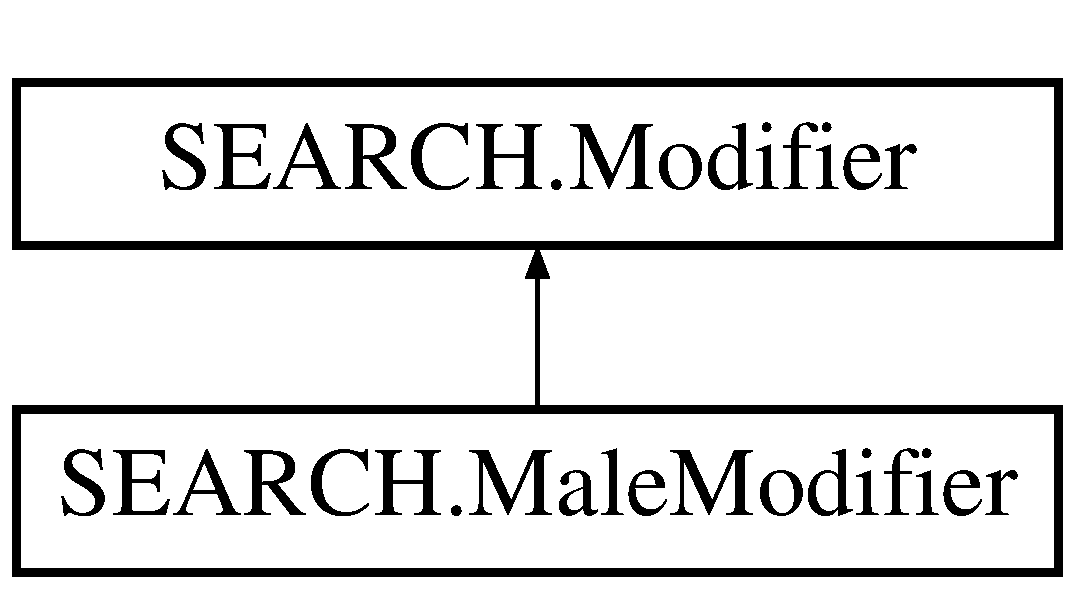
\includegraphics[height=2.000000cm]{class_s_e_a_r_c_h_1_1_male_modifier}
\end{center}
\end{figure}
\subsection*{Static Public Member Functions}
\begin{DoxyCompactItemize}
\item 
static \hyperlink{class_s_e_a_r_c_h_1_1_male_modifier}{Male\-Modifier} \hyperlink{class_s_e_a_r_c_h_1_1_male_modifier_a321255c5bdf156ecf49a594818d66038}{Get\-Unique\-Instance} ()
\begin{DoxyCompactList}\small\item\em -\/\-This operation implements the logic for returning the unique instance of the Singleton pattern. \end{DoxyCompactList}\end{DoxyCompactItemize}
\subsection*{Additional Inherited Members}


\subsection{Detailed Description}
Modifies the animals behavior based on the fact it is a male animal -\/\-The Singleton defines an Instance operation that lets clients access its unique instance. -\/\-It may be responsible for creating its own unique instance. 



\subsection{Member Function Documentation}
\hypertarget{class_s_e_a_r_c_h_1_1_male_modifier_a321255c5bdf156ecf49a594818d66038}{\index{S\-E\-A\-R\-C\-H\-::\-Male\-Modifier@{S\-E\-A\-R\-C\-H\-::\-Male\-Modifier}!Get\-Unique\-Instance@{Get\-Unique\-Instance}}
\index{Get\-Unique\-Instance@{Get\-Unique\-Instance}!SEARCH::MaleModifier@{S\-E\-A\-R\-C\-H\-::\-Male\-Modifier}}
\subsubsection[{Get\-Unique\-Instance}]{\setlength{\rightskip}{0pt plus 5cm}static {\bf Male\-Modifier} S\-E\-A\-R\-C\-H.\-Male\-Modifier.\-Get\-Unique\-Instance (
\begin{DoxyParamCaption}
{}
\end{DoxyParamCaption}
)\hspace{0.3cm}{\ttfamily [static]}}}\label{class_s_e_a_r_c_h_1_1_male_modifier_a321255c5bdf156ecf49a594818d66038}


-\/\-This operation implements the logic for returning the unique instance of the Singleton pattern. 



The documentation for this class was generated from the following file\-:\begin{DoxyCompactItemize}
\item 
Desktop/vlog4net\-A\-R\-C10\-\_\-64\-\_\-newhoming/\-Data\-Centric/\hyperlink{_male_modifier_8cs}{Male\-Modifier.\-cs}\end{DoxyCompactItemize}

\hypertarget{class_s_e_a_r_c_h_1_1_map}{\section{S\-E\-A\-R\-C\-H.\-Map Class Reference}
\label{class_s_e_a_r_c_h_1_1_map}\index{S\-E\-A\-R\-C\-H.\-Map@{S\-E\-A\-R\-C\-H.\-Map}}
}
Inheritance diagram for S\-E\-A\-R\-C\-H.\-Map\-:\begin{figure}[H]
\begin{center}
\leavevmode
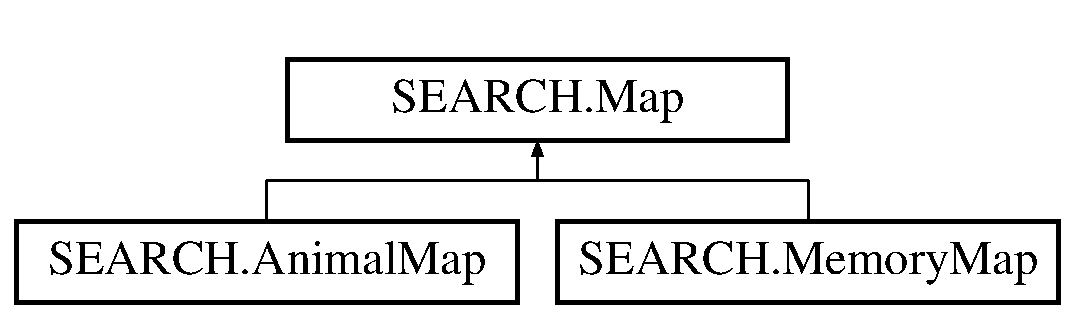
\includegraphics[height=2.000000cm]{class_s_e_a_r_c_h_1_1_map}
\end{center}
\end{figure}
\subsection*{Public Member Functions}
\begin{DoxyCompactItemize}
\item 
\hyperlink{class_s_e_a_r_c_h_1_1_map_a7ecbb3dd1eac1ee71904194f9ca07d9b}{Map} (string path, string file\-Name, I\-Geometry\-Def in\-Geo\-Def, I\-Fields in\-Fields\-Collection)
\item 
\hyperlink{class_s_e_a_r_c_h_1_1_map_a953088c1888b52aeb6e5e3ac07c727d5}{Map} (I\-Feature\-Class in\-Self, string full\-Name)
\item 
\hyperlink{class_s_e_a_r_c_h_1_1_map_af383f58d5e3f9d5c8d7cafc925c8c844}{Map} (I\-Feature\-Class in\-Self)
\item 
\hyperlink{class_s_e_a_r_c_h_1_1_map_a65bef4cc1272ada017b863831191c5e4}{Map} ()
\item 
void \hyperlink{class_s_e_a_r_c_h_1_1_map_a1b2e35d6d5df11469b120c86765d879a}{add\-Day} ()
\item 
void \hyperlink{class_s_e_a_r_c_h_1_1_map_aff5b1e936b7d53be0762ea3d65e5f3f9}{add\-Field} (string name, esri\-Field\-Type type)
\item 
void \hyperlink{class_s_e_a_r_c_h_1_1_map_ad29cd67a27cf5f0ba2957b1c043aea91}{add\-Year} ()
\item 
void \hyperlink{class_s_e_a_r_c_h_1_1_map_a6cfbea6bd3ad958c2e2156c7dc4acc31}{disovle\-Features} (string field\-Name)
\item 
void \hyperlink{class_s_e_a_r_c_h_1_1_map_a59ac519a37e976ad25c39a22fc9ead0f}{dissolve\-Polygons} (string in\-Field\-Name)
\item 
double \hyperlink{class_s_e_a_r_c_h_1_1_map_aeaea5c290cf0e3636e7357d66f54f879}{get\-All\-Available\-Area} (int in\-Animal\-I\-D, string sex)
\item 
Hashtable \hyperlink{class_s_e_a_r_c_h_1_1_map_a4e0fd4f6685b3e2780a04906da471d4b}{get\-All\-Values\-For\-Single\-Polygon} (int in\-Poly\-Index)
\item 
double \hyperlink{class_s_e_a_r_c_h_1_1_map_a242454b3ef52b6e4bb24738379b932e6}{get\-Area} (I\-Point in\-Point)
\item 
double \hyperlink{class_s_e_a_r_c_h_1_1_map_a50856220fecdac4c30dcbb0f65a28ba6}{get\-Available\-Area} (int in\-Poly\-Index)
\item 
\hyperlink{class_s_e_a_r_c_h_1_1cross_over_info}{cross\-Over\-Info} \hyperlink{class_s_e_a_r_c_h_1_1_map_ae0a445111db096d6b6bb09b64cdbbbe4}{get\-Cross\-Over\-Info} (I\-Point start\-Point, I\-Point end\-Point)
\item 
\hyperlink{class_s_e_a_r_c_h_1_1cross_over_info}{cross\-Over\-Info} \hyperlink{class_s_e_a_r_c_h_1_1_map_a8e085c0c103c7bba868cd5ec6dc58576}{get\-Cross\-Over\-Info} (I\-Point start\-Point, I\-Point end\-Point, ref int cur\-Poly\-Index, ref int new\-Poly\-Index)
\item 
int \hyperlink{class_s_e_a_r_c_h_1_1_map_afaf6c24ab8c14ff1c899a331b0af263d}{get\-Current\-Polygon} (I\-Point in\-Point)
\item 
void \hyperlink{class_s_e_a_r_c_h_1_1_map_a1fc41928b46c1c153da6cd9c413a0e0b}{Get\-Initial\-Animal\-Attributes} (out \hyperlink{class_s_e_a_r_c_h_1_1_initial_animal_attributes}{Initial\-Animal\-Attributes}\mbox{[}$\,$\mbox{]} out\-Attributes)
\item 
void \hyperlink{class_s_e_a_r_c_h_1_1_map_a8d92602d25d37e55689650b6729b4404}{Get\-Initial\-Resident\-Information} (out \hyperlink{class_s_e_a_r_c_h_1_1_initial_animal_attributes}{Initial\-Animal\-Attributes}\mbox{[}$\,$\mbox{]} out\-Info)
\item 
I\-Feature\-Layer \hyperlink{class_s_e_a_r_c_h_1_1_map_a98660ce67b8d9d9a47315817e7d09ff6}{get\-Layer} ()
\item 
object \hyperlink{class_s_e_a_r_c_h_1_1_map_a81a287684ca0d411786b71be886fa738}{get\-Named\-Value\-For\-Single\-Polygon} (int in\-Poly\-Index, string in\-Name)
\item 
void \hyperlink{class_s_e_a_r_c_h_1_1_map_aede5d9970e67130ec00d6e39e083caf6}{get\-Num\-Residents} (out int num\-Males, out int num\-Females)
\item 
I\-Table \hyperlink{class_s_e_a_r_c_h_1_1_map_a3ab1be09a8e0f4162c9ca7cd41a38d70}{get\-Table} ()
\item 
I\-Workspace\-Name \hyperlink{class_s_e_a_r_c_h_1_1_map_a78a2dab5002abc586117ea0c578bb9fc}{get\-Workspace\-Name} ()
\item 
bool \hyperlink{class_s_e_a_r_c_h_1_1_map_a728c467f17a14b09253045c0ced6fa79}{has\-Features} ()
\item 
bool \hyperlink{class_s_e_a_r_c_h_1_1_map_a7505c8517f1473cc8fdb67c308a005c6}{is\-Point\-On\-Map} (I\-Point in\-Point)
\item 
bool \hyperlink{class_s_e_a_r_c_h_1_1_map_a0fccbfbd63531ec7bcf6827211f215d3}{point\-In\-Polygon} (I\-Point in\-Point, int in\-Polygon\-Index)
\item 
void \hyperlink{class_s_e_a_r_c_h_1_1_map_a0417e4240959d334d20e22acacb12577}{remove\-All\-Polygons} ()
\item 
void \hyperlink{class_s_e_a_r_c_h_1_1_map_a1897b0a81b39a56adbd3bcd467ba30c4}{remove\-All\-Polygons} (ref I\-Feature\-Class in\-Feature\-Class)
\item 
void \hyperlink{class_s_e_a_r_c_h_1_1_map_a12b9f060fa1a70b29c9856f71559f383}{remove\-Certain\-Polygons} (string field\-Name, string field\-Value)
\item 
void \hyperlink{class_s_e_a_r_c_h_1_1_map_aedc41065fe67279790a7a98ca250d5fd}{reset\-Fields} (string field\-Name, string old\-Value, string new\-Value)
\end{DoxyCompactItemize}
\subsection*{Static Public Member Functions}
\begin{DoxyCompactItemize}
\item 
static I\-Polygon \hyperlink{class_s_e_a_r_c_h_1_1_map_a6a3f3153fc9c97c281a84a88b097291f}{Build\-Home\-Range\-Polygon} (\hyperlink{class_s_e_a_r_c_h_1_1_animal}{Animal} in\-Animal, double stretch\-Factor)
\item 
static I\-Feature\-Class \hyperlink{class_s_e_a_r_c_h_1_1_map_a896a793f7f87aec6339e894e69457e7a}{get\-Map} (string path, string file\-Name)
\item 
static I\-Feature\-Class \hyperlink{class_s_e_a_r_c_h_1_1_map_ada8c27f808eda6bf8db7bf92459b724a}{open\-Feature\-Class} (string path, string file\-Name)
\end{DoxyCompactItemize}
\subsection*{Protected Member Functions}
\begin{DoxyCompactItemize}
\item 
void \hyperlink{class_s_e_a_r_c_h_1_1_map_af4a367d729f5ab652f220804539c1f2c}{build\-Data\-Set\-Name} (string in\-Name)
\item 
void \hyperlink{class_s_e_a_r_c_h_1_1_map_af79f2e8da9452a0d3407327dcb524e93}{build\-Out\-Shape\-File\-Name} ()
\item 
void \hyperlink{class_s_e_a_r_c_h_1_1_map_a9c6b5e23b7fd722b080b437e12a5d55d}{build\-Work\-Space\-Name} ()
\item 
void \hyperlink{class_s_e_a_r_c_h_1_1_map_ad43939d23b677a9f309784a0383f7c68}{get\-Table} (out I\-Table in\-Out\-Table, I\-Feature\-Class in\-Feature\-Class)
\item 
void \hyperlink{class_s_e_a_r_c_h_1_1_map_af8526bf1407a619bd6e54347c65234e9}{remove\-Polygon} (I\-Feature in\-Feature)
\end{DoxyCompactItemize}
\subsection*{Protected Attributes}
\begin{DoxyCompactItemize}
\item 
I\-Dataset\-Name \hyperlink{class_s_e_a_r_c_h_1_1_map_a7574d4bb88c0b061549c9dece3001a23}{ds\-Name}
\item 
I\-Feature\-Class \hyperlink{class_s_e_a_r_c_h_1_1_map_af2222aba365913cbc5c4b2079548c239}{m\-My\-Self}
\item 
string \hyperlink{class_s_e_a_r_c_h_1_1_map_a90d4766a33cf7449b2c8718444529f57}{m\-Type\-Of\-Map}
\item 
I\-Feature\-Layer \hyperlink{class_s_e_a_r_c_h_1_1_map_a9e7228cbe13122db7eaaab6b9d082ee7}{my\-Feature\-Layer}
\item 
string \hyperlink{class_s_e_a_r_c_h_1_1_map_a28f79b85291e056fc85ca8323da61297}{my\-File\-Name}
\item 
string \hyperlink{class_s_e_a_r_c_h_1_1_map_a0f0c4abf19365d8718c41e73deb2aa09}{my\-Path}
\item 
I\-Feature\-Class\-Name \hyperlink{class_s_e_a_r_c_h_1_1_map_a082cc6a38d780c1297092f10539e4cfc}{out\-Shape\-File\-Name}
\item 
I\-Workspace\-Name \hyperlink{class_s_e_a_r_c_h_1_1_map_afe1df1bff77c399788491856548bb3cd}{ws\-Name}
\end{DoxyCompactItemize}
\subsection*{Properties}
\begin{DoxyCompactItemize}
\item 
Date\-Time \hyperlink{class_s_e_a_r_c_h_1_1_map_a4e32fd0cba61fd31d31b23d637a6fdc6}{Begin\-Time}\hspace{0.3cm}{\ttfamily  \mbox{[}get, set\mbox{]}}
\item 
string \hyperlink{class_s_e_a_r_c_h_1_1_map_a25648ab34ea64af19851858a4a4dbebe}{Change\-Type}\hspace{0.3cm}{\ttfamily  \mbox{[}get, set\mbox{]}}
\item 
string \hyperlink{class_s_e_a_r_c_h_1_1_map_a7905b479d4c635fef8133212ec532e3f}{Full\-File\-Name}\hspace{0.3cm}{\ttfamily  \mbox{[}get, set\mbox{]}}
\item 
I\-Feature\-Class \hyperlink{class_s_e_a_r_c_h_1_1_map_a6bb03e540f47336a0eac62a1b73e8cfe}{my\-Self}\hspace{0.3cm}{\ttfamily  \mbox{[}get, set\mbox{]}}
\item 
string \hyperlink{class_s_e_a_r_c_h_1_1_map_a64d3d4785e808bbc15781d2071ff8c3e}{Path}\hspace{0.3cm}{\ttfamily  \mbox{[}get, set\mbox{]}}
\item 
string \hyperlink{class_s_e_a_r_c_h_1_1_map_afa651b1a6b9cc662d4c5b40513cf6906}{Type\-Of\-Map}\hspace{0.3cm}{\ttfamily  \mbox{[}get, set\mbox{]}}
\end{DoxyCompactItemize}


\subsection{Constructor \& Destructor Documentation}
\hypertarget{class_s_e_a_r_c_h_1_1_map_a7ecbb3dd1eac1ee71904194f9ca07d9b}{\index{S\-E\-A\-R\-C\-H\-::\-Map@{S\-E\-A\-R\-C\-H\-::\-Map}!Map@{Map}}
\index{Map@{Map}!SEARCH::Map@{S\-E\-A\-R\-C\-H\-::\-Map}}
\subsubsection[{Map}]{\setlength{\rightskip}{0pt plus 5cm}S\-E\-A\-R\-C\-H.\-Map.\-Map (
\begin{DoxyParamCaption}
\item[{string}]{path, }
\item[{string}]{file\-Name, }
\item[{I\-Geometry\-Def}]{in\-Geo\-Def, }
\item[{I\-Fields}]{in\-Fields\-Collection}
\end{DoxyParamCaption}
)}}\label{class_s_e_a_r_c_h_1_1_map_a7ecbb3dd1eac1ee71904194f9ca07d9b}
\hypertarget{class_s_e_a_r_c_h_1_1_map_a953088c1888b52aeb6e5e3ac07c727d5}{\index{S\-E\-A\-R\-C\-H\-::\-Map@{S\-E\-A\-R\-C\-H\-::\-Map}!Map@{Map}}
\index{Map@{Map}!SEARCH::Map@{S\-E\-A\-R\-C\-H\-::\-Map}}
\subsubsection[{Map}]{\setlength{\rightskip}{0pt plus 5cm}S\-E\-A\-R\-C\-H.\-Map.\-Map (
\begin{DoxyParamCaption}
\item[{I\-Feature\-Class}]{in\-Self, }
\item[{string}]{full\-Name}
\end{DoxyParamCaption}
)}}\label{class_s_e_a_r_c_h_1_1_map_a953088c1888b52aeb6e5e3ac07c727d5}
\hypertarget{class_s_e_a_r_c_h_1_1_map_af383f58d5e3f9d5c8d7cafc925c8c844}{\index{S\-E\-A\-R\-C\-H\-::\-Map@{S\-E\-A\-R\-C\-H\-::\-Map}!Map@{Map}}
\index{Map@{Map}!SEARCH::Map@{S\-E\-A\-R\-C\-H\-::\-Map}}
\subsubsection[{Map}]{\setlength{\rightskip}{0pt plus 5cm}S\-E\-A\-R\-C\-H.\-Map.\-Map (
\begin{DoxyParamCaption}
\item[{I\-Feature\-Class}]{in\-Self}
\end{DoxyParamCaption}
)}}\label{class_s_e_a_r_c_h_1_1_map_af383f58d5e3f9d5c8d7cafc925c8c844}
\hypertarget{class_s_e_a_r_c_h_1_1_map_a65bef4cc1272ada017b863831191c5e4}{\index{S\-E\-A\-R\-C\-H\-::\-Map@{S\-E\-A\-R\-C\-H\-::\-Map}!Map@{Map}}
\index{Map@{Map}!SEARCH::Map@{S\-E\-A\-R\-C\-H\-::\-Map}}
\subsubsection[{Map}]{\setlength{\rightskip}{0pt plus 5cm}S\-E\-A\-R\-C\-H.\-Map.\-Map (
\begin{DoxyParamCaption}
{}
\end{DoxyParamCaption}
)}}\label{class_s_e_a_r_c_h_1_1_map_a65bef4cc1272ada017b863831191c5e4}


\subsection{Member Function Documentation}
\hypertarget{class_s_e_a_r_c_h_1_1_map_a1b2e35d6d5df11469b120c86765d879a}{\index{S\-E\-A\-R\-C\-H\-::\-Map@{S\-E\-A\-R\-C\-H\-::\-Map}!add\-Day@{add\-Day}}
\index{add\-Day@{add\-Day}!SEARCH::Map@{S\-E\-A\-R\-C\-H\-::\-Map}}
\subsubsection[{add\-Day}]{\setlength{\rightskip}{0pt plus 5cm}void S\-E\-A\-R\-C\-H.\-Map.\-add\-Day (
\begin{DoxyParamCaption}
{}
\end{DoxyParamCaption}
)}}\label{class_s_e_a_r_c_h_1_1_map_a1b2e35d6d5df11469b120c86765d879a}
\hypertarget{class_s_e_a_r_c_h_1_1_map_aff5b1e936b7d53be0762ea3d65e5f3f9}{\index{S\-E\-A\-R\-C\-H\-::\-Map@{S\-E\-A\-R\-C\-H\-::\-Map}!add\-Field@{add\-Field}}
\index{add\-Field@{add\-Field}!SEARCH::Map@{S\-E\-A\-R\-C\-H\-::\-Map}}
\subsubsection[{add\-Field}]{\setlength{\rightskip}{0pt plus 5cm}void S\-E\-A\-R\-C\-H.\-Map.\-add\-Field (
\begin{DoxyParamCaption}
\item[{string}]{name, }
\item[{esri\-Field\-Type}]{type}
\end{DoxyParamCaption}
)}}\label{class_s_e_a_r_c_h_1_1_map_aff5b1e936b7d53be0762ea3d65e5f3f9}
\hypertarget{class_s_e_a_r_c_h_1_1_map_ad29cd67a27cf5f0ba2957b1c043aea91}{\index{S\-E\-A\-R\-C\-H\-::\-Map@{S\-E\-A\-R\-C\-H\-::\-Map}!add\-Year@{add\-Year}}
\index{add\-Year@{add\-Year}!SEARCH::Map@{S\-E\-A\-R\-C\-H\-::\-Map}}
\subsubsection[{add\-Year}]{\setlength{\rightskip}{0pt plus 5cm}void S\-E\-A\-R\-C\-H.\-Map.\-add\-Year (
\begin{DoxyParamCaption}
{}
\end{DoxyParamCaption}
)}}\label{class_s_e_a_r_c_h_1_1_map_ad29cd67a27cf5f0ba2957b1c043aea91}
\hypertarget{class_s_e_a_r_c_h_1_1_map_af4a367d729f5ab652f220804539c1f2c}{\index{S\-E\-A\-R\-C\-H\-::\-Map@{S\-E\-A\-R\-C\-H\-::\-Map}!build\-Data\-Set\-Name@{build\-Data\-Set\-Name}}
\index{build\-Data\-Set\-Name@{build\-Data\-Set\-Name}!SEARCH::Map@{S\-E\-A\-R\-C\-H\-::\-Map}}
\subsubsection[{build\-Data\-Set\-Name}]{\setlength{\rightskip}{0pt plus 5cm}void S\-E\-A\-R\-C\-H.\-Map.\-build\-Data\-Set\-Name (
\begin{DoxyParamCaption}
\item[{string}]{in\-Name}
\end{DoxyParamCaption}
)\hspace{0.3cm}{\ttfamily [protected]}}}\label{class_s_e_a_r_c_h_1_1_map_af4a367d729f5ab652f220804539c1f2c}
\hypertarget{class_s_e_a_r_c_h_1_1_map_a6a3f3153fc9c97c281a84a88b097291f}{\index{S\-E\-A\-R\-C\-H\-::\-Map@{S\-E\-A\-R\-C\-H\-::\-Map}!Build\-Home\-Range\-Polygon@{Build\-Home\-Range\-Polygon}}
\index{Build\-Home\-Range\-Polygon@{Build\-Home\-Range\-Polygon}!SEARCH::Map@{S\-E\-A\-R\-C\-H\-::\-Map}}
\subsubsection[{Build\-Home\-Range\-Polygon}]{\setlength{\rightskip}{0pt plus 5cm}static I\-Polygon S\-E\-A\-R\-C\-H.\-Map.\-Build\-Home\-Range\-Polygon (
\begin{DoxyParamCaption}
\item[{{\bf Animal}}]{in\-Animal, }
\item[{double}]{stretch\-Factor}
\end{DoxyParamCaption}
)\hspace{0.3cm}{\ttfamily [static]}}}\label{class_s_e_a_r_c_h_1_1_map_a6a3f3153fc9c97c281a84a88b097291f}
\hypertarget{class_s_e_a_r_c_h_1_1_map_af79f2e8da9452a0d3407327dcb524e93}{\index{S\-E\-A\-R\-C\-H\-::\-Map@{S\-E\-A\-R\-C\-H\-::\-Map}!build\-Out\-Shape\-File\-Name@{build\-Out\-Shape\-File\-Name}}
\index{build\-Out\-Shape\-File\-Name@{build\-Out\-Shape\-File\-Name}!SEARCH::Map@{S\-E\-A\-R\-C\-H\-::\-Map}}
\subsubsection[{build\-Out\-Shape\-File\-Name}]{\setlength{\rightskip}{0pt plus 5cm}void S\-E\-A\-R\-C\-H.\-Map.\-build\-Out\-Shape\-File\-Name (
\begin{DoxyParamCaption}
{}
\end{DoxyParamCaption}
)\hspace{0.3cm}{\ttfamily [protected]}}}\label{class_s_e_a_r_c_h_1_1_map_af79f2e8da9452a0d3407327dcb524e93}
\hypertarget{class_s_e_a_r_c_h_1_1_map_a9c6b5e23b7fd722b080b437e12a5d55d}{\index{S\-E\-A\-R\-C\-H\-::\-Map@{S\-E\-A\-R\-C\-H\-::\-Map}!build\-Work\-Space\-Name@{build\-Work\-Space\-Name}}
\index{build\-Work\-Space\-Name@{build\-Work\-Space\-Name}!SEARCH::Map@{S\-E\-A\-R\-C\-H\-::\-Map}}
\subsubsection[{build\-Work\-Space\-Name}]{\setlength{\rightskip}{0pt plus 5cm}void S\-E\-A\-R\-C\-H.\-Map.\-build\-Work\-Space\-Name (
\begin{DoxyParamCaption}
{}
\end{DoxyParamCaption}
)\hspace{0.3cm}{\ttfamily [protected]}}}\label{class_s_e_a_r_c_h_1_1_map_a9c6b5e23b7fd722b080b437e12a5d55d}
\hypertarget{class_s_e_a_r_c_h_1_1_map_a6cfbea6bd3ad958c2e2156c7dc4acc31}{\index{S\-E\-A\-R\-C\-H\-::\-Map@{S\-E\-A\-R\-C\-H\-::\-Map}!disovle\-Features@{disovle\-Features}}
\index{disovle\-Features@{disovle\-Features}!SEARCH::Map@{S\-E\-A\-R\-C\-H\-::\-Map}}
\subsubsection[{disovle\-Features}]{\setlength{\rightskip}{0pt plus 5cm}void S\-E\-A\-R\-C\-H.\-Map.\-disovle\-Features (
\begin{DoxyParamCaption}
\item[{string}]{field\-Name}
\end{DoxyParamCaption}
)}}\label{class_s_e_a_r_c_h_1_1_map_a6cfbea6bd3ad958c2e2156c7dc4acc31}
\hypertarget{class_s_e_a_r_c_h_1_1_map_a59ac519a37e976ad25c39a22fc9ead0f}{\index{S\-E\-A\-R\-C\-H\-::\-Map@{S\-E\-A\-R\-C\-H\-::\-Map}!dissolve\-Polygons@{dissolve\-Polygons}}
\index{dissolve\-Polygons@{dissolve\-Polygons}!SEARCH::Map@{S\-E\-A\-R\-C\-H\-::\-Map}}
\subsubsection[{dissolve\-Polygons}]{\setlength{\rightskip}{0pt plus 5cm}void S\-E\-A\-R\-C\-H.\-Map.\-dissolve\-Polygons (
\begin{DoxyParamCaption}
\item[{string}]{in\-Field\-Name}
\end{DoxyParamCaption}
)}}\label{class_s_e_a_r_c_h_1_1_map_a59ac519a37e976ad25c39a22fc9ead0f}
\hypertarget{class_s_e_a_r_c_h_1_1_map_aeaea5c290cf0e3636e7357d66f54f879}{\index{S\-E\-A\-R\-C\-H\-::\-Map@{S\-E\-A\-R\-C\-H\-::\-Map}!get\-All\-Available\-Area@{get\-All\-Available\-Area}}
\index{get\-All\-Available\-Area@{get\-All\-Available\-Area}!SEARCH::Map@{S\-E\-A\-R\-C\-H\-::\-Map}}
\subsubsection[{get\-All\-Available\-Area}]{\setlength{\rightskip}{0pt plus 5cm}double S\-E\-A\-R\-C\-H.\-Map.\-get\-All\-Available\-Area (
\begin{DoxyParamCaption}
\item[{int}]{in\-Animal\-I\-D, }
\item[{string}]{sex}
\end{DoxyParamCaption}
)}}\label{class_s_e_a_r_c_h_1_1_map_aeaea5c290cf0e3636e7357d66f54f879}
\hypertarget{class_s_e_a_r_c_h_1_1_map_a4e0fd4f6685b3e2780a04906da471d4b}{\index{S\-E\-A\-R\-C\-H\-::\-Map@{S\-E\-A\-R\-C\-H\-::\-Map}!get\-All\-Values\-For\-Single\-Polygon@{get\-All\-Values\-For\-Single\-Polygon}}
\index{get\-All\-Values\-For\-Single\-Polygon@{get\-All\-Values\-For\-Single\-Polygon}!SEARCH::Map@{S\-E\-A\-R\-C\-H\-::\-Map}}
\subsubsection[{get\-All\-Values\-For\-Single\-Polygon}]{\setlength{\rightskip}{0pt plus 5cm}Hashtable S\-E\-A\-R\-C\-H.\-Map.\-get\-All\-Values\-For\-Single\-Polygon (
\begin{DoxyParamCaption}
\item[{int}]{in\-Poly\-Index}
\end{DoxyParamCaption}
)}}\label{class_s_e_a_r_c_h_1_1_map_a4e0fd4f6685b3e2780a04906da471d4b}
\hypertarget{class_s_e_a_r_c_h_1_1_map_a242454b3ef52b6e4bb24738379b932e6}{\index{S\-E\-A\-R\-C\-H\-::\-Map@{S\-E\-A\-R\-C\-H\-::\-Map}!get\-Area@{get\-Area}}
\index{get\-Area@{get\-Area}!SEARCH::Map@{S\-E\-A\-R\-C\-H\-::\-Map}}
\subsubsection[{get\-Area}]{\setlength{\rightskip}{0pt plus 5cm}double S\-E\-A\-R\-C\-H.\-Map.\-get\-Area (
\begin{DoxyParamCaption}
\item[{I\-Point}]{in\-Point}
\end{DoxyParamCaption}
)}}\label{class_s_e_a_r_c_h_1_1_map_a242454b3ef52b6e4bb24738379b932e6}
\hypertarget{class_s_e_a_r_c_h_1_1_map_a50856220fecdac4c30dcbb0f65a28ba6}{\index{S\-E\-A\-R\-C\-H\-::\-Map@{S\-E\-A\-R\-C\-H\-::\-Map}!get\-Available\-Area@{get\-Available\-Area}}
\index{get\-Available\-Area@{get\-Available\-Area}!SEARCH::Map@{S\-E\-A\-R\-C\-H\-::\-Map}}
\subsubsection[{get\-Available\-Area}]{\setlength{\rightskip}{0pt plus 5cm}double S\-E\-A\-R\-C\-H.\-Map.\-get\-Available\-Area (
\begin{DoxyParamCaption}
\item[{int}]{in\-Poly\-Index}
\end{DoxyParamCaption}
)}}\label{class_s_e_a_r_c_h_1_1_map_a50856220fecdac4c30dcbb0f65a28ba6}
\hypertarget{class_s_e_a_r_c_h_1_1_map_ae0a445111db096d6b6bb09b64cdbbbe4}{\index{S\-E\-A\-R\-C\-H\-::\-Map@{S\-E\-A\-R\-C\-H\-::\-Map}!get\-Cross\-Over\-Info@{get\-Cross\-Over\-Info}}
\index{get\-Cross\-Over\-Info@{get\-Cross\-Over\-Info}!SEARCH::Map@{S\-E\-A\-R\-C\-H\-::\-Map}}
\subsubsection[{get\-Cross\-Over\-Info}]{\setlength{\rightskip}{0pt plus 5cm}{\bf cross\-Over\-Info} S\-E\-A\-R\-C\-H.\-Map.\-get\-Cross\-Over\-Info (
\begin{DoxyParamCaption}
\item[{I\-Point}]{start\-Point, }
\item[{I\-Point}]{end\-Point}
\end{DoxyParamCaption}
)}}\label{class_s_e_a_r_c_h_1_1_map_ae0a445111db096d6b6bb09b64cdbbbe4}
\hypertarget{class_s_e_a_r_c_h_1_1_map_a8e085c0c103c7bba868cd5ec6dc58576}{\index{S\-E\-A\-R\-C\-H\-::\-Map@{S\-E\-A\-R\-C\-H\-::\-Map}!get\-Cross\-Over\-Info@{get\-Cross\-Over\-Info}}
\index{get\-Cross\-Over\-Info@{get\-Cross\-Over\-Info}!SEARCH::Map@{S\-E\-A\-R\-C\-H\-::\-Map}}
\subsubsection[{get\-Cross\-Over\-Info}]{\setlength{\rightskip}{0pt plus 5cm}{\bf cross\-Over\-Info} S\-E\-A\-R\-C\-H.\-Map.\-get\-Cross\-Over\-Info (
\begin{DoxyParamCaption}
\item[{I\-Point}]{start\-Point, }
\item[{I\-Point}]{end\-Point, }
\item[{ref int}]{cur\-Poly\-Index, }
\item[{ref int}]{new\-Poly\-Index}
\end{DoxyParamCaption}
)}}\label{class_s_e_a_r_c_h_1_1_map_a8e085c0c103c7bba868cd5ec6dc58576}
\hypertarget{class_s_e_a_r_c_h_1_1_map_afaf6c24ab8c14ff1c899a331b0af263d}{\index{S\-E\-A\-R\-C\-H\-::\-Map@{S\-E\-A\-R\-C\-H\-::\-Map}!get\-Current\-Polygon@{get\-Current\-Polygon}}
\index{get\-Current\-Polygon@{get\-Current\-Polygon}!SEARCH::Map@{S\-E\-A\-R\-C\-H\-::\-Map}}
\subsubsection[{get\-Current\-Polygon}]{\setlength{\rightskip}{0pt plus 5cm}int S\-E\-A\-R\-C\-H.\-Map.\-get\-Current\-Polygon (
\begin{DoxyParamCaption}
\item[{I\-Point}]{in\-Point}
\end{DoxyParamCaption}
)}}\label{class_s_e_a_r_c_h_1_1_map_afaf6c24ab8c14ff1c899a331b0af263d}
\hypertarget{class_s_e_a_r_c_h_1_1_map_a1fc41928b46c1c153da6cd9c413a0e0b}{\index{S\-E\-A\-R\-C\-H\-::\-Map@{S\-E\-A\-R\-C\-H\-::\-Map}!Get\-Initial\-Animal\-Attributes@{Get\-Initial\-Animal\-Attributes}}
\index{Get\-Initial\-Animal\-Attributes@{Get\-Initial\-Animal\-Attributes}!SEARCH::Map@{S\-E\-A\-R\-C\-H\-::\-Map}}
\subsubsection[{Get\-Initial\-Animal\-Attributes}]{\setlength{\rightskip}{0pt plus 5cm}void S\-E\-A\-R\-C\-H.\-Map.\-Get\-Initial\-Animal\-Attributes (
\begin{DoxyParamCaption}
\item[{out {\bf Initial\-Animal\-Attributes}\mbox{[}$\,$\mbox{]}}]{out\-Attributes}
\end{DoxyParamCaption}
)}}\label{class_s_e_a_r_c_h_1_1_map_a1fc41928b46c1c153da6cd9c413a0e0b}
\hypertarget{class_s_e_a_r_c_h_1_1_map_a8d92602d25d37e55689650b6729b4404}{\index{S\-E\-A\-R\-C\-H\-::\-Map@{S\-E\-A\-R\-C\-H\-::\-Map}!Get\-Initial\-Resident\-Information@{Get\-Initial\-Resident\-Information}}
\index{Get\-Initial\-Resident\-Information@{Get\-Initial\-Resident\-Information}!SEARCH::Map@{S\-E\-A\-R\-C\-H\-::\-Map}}
\subsubsection[{Get\-Initial\-Resident\-Information}]{\setlength{\rightskip}{0pt plus 5cm}void S\-E\-A\-R\-C\-H.\-Map.\-Get\-Initial\-Resident\-Information (
\begin{DoxyParamCaption}
\item[{out {\bf Initial\-Animal\-Attributes}\mbox{[}$\,$\mbox{]}}]{out\-Info}
\end{DoxyParamCaption}
)}}\label{class_s_e_a_r_c_h_1_1_map_a8d92602d25d37e55689650b6729b4404}
\hypertarget{class_s_e_a_r_c_h_1_1_map_a98660ce67b8d9d9a47315817e7d09ff6}{\index{S\-E\-A\-R\-C\-H\-::\-Map@{S\-E\-A\-R\-C\-H\-::\-Map}!get\-Layer@{get\-Layer}}
\index{get\-Layer@{get\-Layer}!SEARCH::Map@{S\-E\-A\-R\-C\-H\-::\-Map}}
\subsubsection[{get\-Layer}]{\setlength{\rightskip}{0pt plus 5cm}I\-Feature\-Layer S\-E\-A\-R\-C\-H.\-Map.\-get\-Layer (
\begin{DoxyParamCaption}
{}
\end{DoxyParamCaption}
)}}\label{class_s_e_a_r_c_h_1_1_map_a98660ce67b8d9d9a47315817e7d09ff6}
\hypertarget{class_s_e_a_r_c_h_1_1_map_a896a793f7f87aec6339e894e69457e7a}{\index{S\-E\-A\-R\-C\-H\-::\-Map@{S\-E\-A\-R\-C\-H\-::\-Map}!get\-Map@{get\-Map}}
\index{get\-Map@{get\-Map}!SEARCH::Map@{S\-E\-A\-R\-C\-H\-::\-Map}}
\subsubsection[{get\-Map}]{\setlength{\rightskip}{0pt plus 5cm}static I\-Feature\-Class S\-E\-A\-R\-C\-H.\-Map.\-get\-Map (
\begin{DoxyParamCaption}
\item[{string}]{path, }
\item[{string}]{file\-Name}
\end{DoxyParamCaption}
)\hspace{0.3cm}{\ttfamily [static]}}}\label{class_s_e_a_r_c_h_1_1_map_a896a793f7f87aec6339e894e69457e7a}
\hypertarget{class_s_e_a_r_c_h_1_1_map_a81a287684ca0d411786b71be886fa738}{\index{S\-E\-A\-R\-C\-H\-::\-Map@{S\-E\-A\-R\-C\-H\-::\-Map}!get\-Named\-Value\-For\-Single\-Polygon@{get\-Named\-Value\-For\-Single\-Polygon}}
\index{get\-Named\-Value\-For\-Single\-Polygon@{get\-Named\-Value\-For\-Single\-Polygon}!SEARCH::Map@{S\-E\-A\-R\-C\-H\-::\-Map}}
\subsubsection[{get\-Named\-Value\-For\-Single\-Polygon}]{\setlength{\rightskip}{0pt plus 5cm}object S\-E\-A\-R\-C\-H.\-Map.\-get\-Named\-Value\-For\-Single\-Polygon (
\begin{DoxyParamCaption}
\item[{int}]{in\-Poly\-Index, }
\item[{string}]{in\-Name}
\end{DoxyParamCaption}
)}}\label{class_s_e_a_r_c_h_1_1_map_a81a287684ca0d411786b71be886fa738}
\hypertarget{class_s_e_a_r_c_h_1_1_map_aede5d9970e67130ec00d6e39e083caf6}{\index{S\-E\-A\-R\-C\-H\-::\-Map@{S\-E\-A\-R\-C\-H\-::\-Map}!get\-Num\-Residents@{get\-Num\-Residents}}
\index{get\-Num\-Residents@{get\-Num\-Residents}!SEARCH::Map@{S\-E\-A\-R\-C\-H\-::\-Map}}
\subsubsection[{get\-Num\-Residents}]{\setlength{\rightskip}{0pt plus 5cm}void S\-E\-A\-R\-C\-H.\-Map.\-get\-Num\-Residents (
\begin{DoxyParamCaption}
\item[{out int}]{num\-Males, }
\item[{out int}]{num\-Females}
\end{DoxyParamCaption}
)}}\label{class_s_e_a_r_c_h_1_1_map_aede5d9970e67130ec00d6e39e083caf6}
\hypertarget{class_s_e_a_r_c_h_1_1_map_a3ab1be09a8e0f4162c9ca7cd41a38d70}{\index{S\-E\-A\-R\-C\-H\-::\-Map@{S\-E\-A\-R\-C\-H\-::\-Map}!get\-Table@{get\-Table}}
\index{get\-Table@{get\-Table}!SEARCH::Map@{S\-E\-A\-R\-C\-H\-::\-Map}}
\subsubsection[{get\-Table}]{\setlength{\rightskip}{0pt plus 5cm}I\-Table S\-E\-A\-R\-C\-H.\-Map.\-get\-Table (
\begin{DoxyParamCaption}
{}
\end{DoxyParamCaption}
)}}\label{class_s_e_a_r_c_h_1_1_map_a3ab1be09a8e0f4162c9ca7cd41a38d70}
\hypertarget{class_s_e_a_r_c_h_1_1_map_ad43939d23b677a9f309784a0383f7c68}{\index{S\-E\-A\-R\-C\-H\-::\-Map@{S\-E\-A\-R\-C\-H\-::\-Map}!get\-Table@{get\-Table}}
\index{get\-Table@{get\-Table}!SEARCH::Map@{S\-E\-A\-R\-C\-H\-::\-Map}}
\subsubsection[{get\-Table}]{\setlength{\rightskip}{0pt plus 5cm}void S\-E\-A\-R\-C\-H.\-Map.\-get\-Table (
\begin{DoxyParamCaption}
\item[{out I\-Table}]{in\-Out\-Table, }
\item[{I\-Feature\-Class}]{in\-Feature\-Class}
\end{DoxyParamCaption}
)\hspace{0.3cm}{\ttfamily [protected]}}}\label{class_s_e_a_r_c_h_1_1_map_ad43939d23b677a9f309784a0383f7c68}
\hypertarget{class_s_e_a_r_c_h_1_1_map_a78a2dab5002abc586117ea0c578bb9fc}{\index{S\-E\-A\-R\-C\-H\-::\-Map@{S\-E\-A\-R\-C\-H\-::\-Map}!get\-Workspace\-Name@{get\-Workspace\-Name}}
\index{get\-Workspace\-Name@{get\-Workspace\-Name}!SEARCH::Map@{S\-E\-A\-R\-C\-H\-::\-Map}}
\subsubsection[{get\-Workspace\-Name}]{\setlength{\rightskip}{0pt plus 5cm}I\-Workspace\-Name S\-E\-A\-R\-C\-H.\-Map.\-get\-Workspace\-Name (
\begin{DoxyParamCaption}
{}
\end{DoxyParamCaption}
)}}\label{class_s_e_a_r_c_h_1_1_map_a78a2dab5002abc586117ea0c578bb9fc}
\hypertarget{class_s_e_a_r_c_h_1_1_map_a728c467f17a14b09253045c0ced6fa79}{\index{S\-E\-A\-R\-C\-H\-::\-Map@{S\-E\-A\-R\-C\-H\-::\-Map}!has\-Features@{has\-Features}}
\index{has\-Features@{has\-Features}!SEARCH::Map@{S\-E\-A\-R\-C\-H\-::\-Map}}
\subsubsection[{has\-Features}]{\setlength{\rightskip}{0pt plus 5cm}bool S\-E\-A\-R\-C\-H.\-Map.\-has\-Features (
\begin{DoxyParamCaption}
{}
\end{DoxyParamCaption}
)}}\label{class_s_e_a_r_c_h_1_1_map_a728c467f17a14b09253045c0ced6fa79}
\hypertarget{class_s_e_a_r_c_h_1_1_map_a7505c8517f1473cc8fdb67c308a005c6}{\index{S\-E\-A\-R\-C\-H\-::\-Map@{S\-E\-A\-R\-C\-H\-::\-Map}!is\-Point\-On\-Map@{is\-Point\-On\-Map}}
\index{is\-Point\-On\-Map@{is\-Point\-On\-Map}!SEARCH::Map@{S\-E\-A\-R\-C\-H\-::\-Map}}
\subsubsection[{is\-Point\-On\-Map}]{\setlength{\rightskip}{0pt plus 5cm}bool S\-E\-A\-R\-C\-H.\-Map.\-is\-Point\-On\-Map (
\begin{DoxyParamCaption}
\item[{I\-Point}]{in\-Point}
\end{DoxyParamCaption}
)}}\label{class_s_e_a_r_c_h_1_1_map_a7505c8517f1473cc8fdb67c308a005c6}
\hypertarget{class_s_e_a_r_c_h_1_1_map_ada8c27f808eda6bf8db7bf92459b724a}{\index{S\-E\-A\-R\-C\-H\-::\-Map@{S\-E\-A\-R\-C\-H\-::\-Map}!open\-Feature\-Class@{open\-Feature\-Class}}
\index{open\-Feature\-Class@{open\-Feature\-Class}!SEARCH::Map@{S\-E\-A\-R\-C\-H\-::\-Map}}
\subsubsection[{open\-Feature\-Class}]{\setlength{\rightskip}{0pt plus 5cm}static I\-Feature\-Class S\-E\-A\-R\-C\-H.\-Map.\-open\-Feature\-Class (
\begin{DoxyParamCaption}
\item[{string}]{path, }
\item[{string}]{file\-Name}
\end{DoxyParamCaption}
)\hspace{0.3cm}{\ttfamily [static]}}}\label{class_s_e_a_r_c_h_1_1_map_ada8c27f808eda6bf8db7bf92459b724a}
\hypertarget{class_s_e_a_r_c_h_1_1_map_a0fccbfbd63531ec7bcf6827211f215d3}{\index{S\-E\-A\-R\-C\-H\-::\-Map@{S\-E\-A\-R\-C\-H\-::\-Map}!point\-In\-Polygon@{point\-In\-Polygon}}
\index{point\-In\-Polygon@{point\-In\-Polygon}!SEARCH::Map@{S\-E\-A\-R\-C\-H\-::\-Map}}
\subsubsection[{point\-In\-Polygon}]{\setlength{\rightskip}{0pt plus 5cm}bool S\-E\-A\-R\-C\-H.\-Map.\-point\-In\-Polygon (
\begin{DoxyParamCaption}
\item[{I\-Point}]{in\-Point, }
\item[{int}]{in\-Polygon\-Index}
\end{DoxyParamCaption}
)}}\label{class_s_e_a_r_c_h_1_1_map_a0fccbfbd63531ec7bcf6827211f215d3}
\hypertarget{class_s_e_a_r_c_h_1_1_map_a0417e4240959d334d20e22acacb12577}{\index{S\-E\-A\-R\-C\-H\-::\-Map@{S\-E\-A\-R\-C\-H\-::\-Map}!remove\-All\-Polygons@{remove\-All\-Polygons}}
\index{remove\-All\-Polygons@{remove\-All\-Polygons}!SEARCH::Map@{S\-E\-A\-R\-C\-H\-::\-Map}}
\subsubsection[{remove\-All\-Polygons}]{\setlength{\rightskip}{0pt plus 5cm}void S\-E\-A\-R\-C\-H.\-Map.\-remove\-All\-Polygons (
\begin{DoxyParamCaption}
{}
\end{DoxyParamCaption}
)}}\label{class_s_e_a_r_c_h_1_1_map_a0417e4240959d334d20e22acacb12577}
\hypertarget{class_s_e_a_r_c_h_1_1_map_a1897b0a81b39a56adbd3bcd467ba30c4}{\index{S\-E\-A\-R\-C\-H\-::\-Map@{S\-E\-A\-R\-C\-H\-::\-Map}!remove\-All\-Polygons@{remove\-All\-Polygons}}
\index{remove\-All\-Polygons@{remove\-All\-Polygons}!SEARCH::Map@{S\-E\-A\-R\-C\-H\-::\-Map}}
\subsubsection[{remove\-All\-Polygons}]{\setlength{\rightskip}{0pt plus 5cm}void S\-E\-A\-R\-C\-H.\-Map.\-remove\-All\-Polygons (
\begin{DoxyParamCaption}
\item[{ref I\-Feature\-Class}]{in\-Feature\-Class}
\end{DoxyParamCaption}
)}}\label{class_s_e_a_r_c_h_1_1_map_a1897b0a81b39a56adbd3bcd467ba30c4}
\hypertarget{class_s_e_a_r_c_h_1_1_map_a12b9f060fa1a70b29c9856f71559f383}{\index{S\-E\-A\-R\-C\-H\-::\-Map@{S\-E\-A\-R\-C\-H\-::\-Map}!remove\-Certain\-Polygons@{remove\-Certain\-Polygons}}
\index{remove\-Certain\-Polygons@{remove\-Certain\-Polygons}!SEARCH::Map@{S\-E\-A\-R\-C\-H\-::\-Map}}
\subsubsection[{remove\-Certain\-Polygons}]{\setlength{\rightskip}{0pt plus 5cm}void S\-E\-A\-R\-C\-H.\-Map.\-remove\-Certain\-Polygons (
\begin{DoxyParamCaption}
\item[{string}]{field\-Name, }
\item[{string}]{field\-Value}
\end{DoxyParamCaption}
)}}\label{class_s_e_a_r_c_h_1_1_map_a12b9f060fa1a70b29c9856f71559f383}
\hypertarget{class_s_e_a_r_c_h_1_1_map_af8526bf1407a619bd6e54347c65234e9}{\index{S\-E\-A\-R\-C\-H\-::\-Map@{S\-E\-A\-R\-C\-H\-::\-Map}!remove\-Polygon@{remove\-Polygon}}
\index{remove\-Polygon@{remove\-Polygon}!SEARCH::Map@{S\-E\-A\-R\-C\-H\-::\-Map}}
\subsubsection[{remove\-Polygon}]{\setlength{\rightskip}{0pt plus 5cm}void S\-E\-A\-R\-C\-H.\-Map.\-remove\-Polygon (
\begin{DoxyParamCaption}
\item[{I\-Feature}]{in\-Feature}
\end{DoxyParamCaption}
)\hspace{0.3cm}{\ttfamily [protected]}}}\label{class_s_e_a_r_c_h_1_1_map_af8526bf1407a619bd6e54347c65234e9}
\hypertarget{class_s_e_a_r_c_h_1_1_map_aedc41065fe67279790a7a98ca250d5fd}{\index{S\-E\-A\-R\-C\-H\-::\-Map@{S\-E\-A\-R\-C\-H\-::\-Map}!reset\-Fields@{reset\-Fields}}
\index{reset\-Fields@{reset\-Fields}!SEARCH::Map@{S\-E\-A\-R\-C\-H\-::\-Map}}
\subsubsection[{reset\-Fields}]{\setlength{\rightskip}{0pt plus 5cm}void S\-E\-A\-R\-C\-H.\-Map.\-reset\-Fields (
\begin{DoxyParamCaption}
\item[{string}]{field\-Name, }
\item[{string}]{old\-Value, }
\item[{string}]{new\-Value}
\end{DoxyParamCaption}
)}}\label{class_s_e_a_r_c_h_1_1_map_aedc41065fe67279790a7a98ca250d5fd}


\subsection{Member Data Documentation}
\hypertarget{class_s_e_a_r_c_h_1_1_map_a7574d4bb88c0b061549c9dece3001a23}{\index{S\-E\-A\-R\-C\-H\-::\-Map@{S\-E\-A\-R\-C\-H\-::\-Map}!ds\-Name@{ds\-Name}}
\index{ds\-Name@{ds\-Name}!SEARCH::Map@{S\-E\-A\-R\-C\-H\-::\-Map}}
\subsubsection[{ds\-Name}]{\setlength{\rightskip}{0pt plus 5cm}I\-Dataset\-Name S\-E\-A\-R\-C\-H.\-Map.\-ds\-Name\hspace{0.3cm}{\ttfamily [protected]}}}\label{class_s_e_a_r_c_h_1_1_map_a7574d4bb88c0b061549c9dece3001a23}
\hypertarget{class_s_e_a_r_c_h_1_1_map_af2222aba365913cbc5c4b2079548c239}{\index{S\-E\-A\-R\-C\-H\-::\-Map@{S\-E\-A\-R\-C\-H\-::\-Map}!m\-My\-Self@{m\-My\-Self}}
\index{m\-My\-Self@{m\-My\-Self}!SEARCH::Map@{S\-E\-A\-R\-C\-H\-::\-Map}}
\subsubsection[{m\-My\-Self}]{\setlength{\rightskip}{0pt plus 5cm}I\-Feature\-Class S\-E\-A\-R\-C\-H.\-Map.\-m\-My\-Self\hspace{0.3cm}{\ttfamily [protected]}}}\label{class_s_e_a_r_c_h_1_1_map_af2222aba365913cbc5c4b2079548c239}
\hypertarget{class_s_e_a_r_c_h_1_1_map_a90d4766a33cf7449b2c8718444529f57}{\index{S\-E\-A\-R\-C\-H\-::\-Map@{S\-E\-A\-R\-C\-H\-::\-Map}!m\-Type\-Of\-Map@{m\-Type\-Of\-Map}}
\index{m\-Type\-Of\-Map@{m\-Type\-Of\-Map}!SEARCH::Map@{S\-E\-A\-R\-C\-H\-::\-Map}}
\subsubsection[{m\-Type\-Of\-Map}]{\setlength{\rightskip}{0pt plus 5cm}string S\-E\-A\-R\-C\-H.\-Map.\-m\-Type\-Of\-Map\hspace{0.3cm}{\ttfamily [protected]}}}\label{class_s_e_a_r_c_h_1_1_map_a90d4766a33cf7449b2c8718444529f57}
\hypertarget{class_s_e_a_r_c_h_1_1_map_a9e7228cbe13122db7eaaab6b9d082ee7}{\index{S\-E\-A\-R\-C\-H\-::\-Map@{S\-E\-A\-R\-C\-H\-::\-Map}!my\-Feature\-Layer@{my\-Feature\-Layer}}
\index{my\-Feature\-Layer@{my\-Feature\-Layer}!SEARCH::Map@{S\-E\-A\-R\-C\-H\-::\-Map}}
\subsubsection[{my\-Feature\-Layer}]{\setlength{\rightskip}{0pt plus 5cm}I\-Feature\-Layer S\-E\-A\-R\-C\-H.\-Map.\-my\-Feature\-Layer\hspace{0.3cm}{\ttfamily [protected]}}}\label{class_s_e_a_r_c_h_1_1_map_a9e7228cbe13122db7eaaab6b9d082ee7}
\hypertarget{class_s_e_a_r_c_h_1_1_map_a28f79b85291e056fc85ca8323da61297}{\index{S\-E\-A\-R\-C\-H\-::\-Map@{S\-E\-A\-R\-C\-H\-::\-Map}!my\-File\-Name@{my\-File\-Name}}
\index{my\-File\-Name@{my\-File\-Name}!SEARCH::Map@{S\-E\-A\-R\-C\-H\-::\-Map}}
\subsubsection[{my\-File\-Name}]{\setlength{\rightskip}{0pt plus 5cm}string S\-E\-A\-R\-C\-H.\-Map.\-my\-File\-Name\hspace{0.3cm}{\ttfamily [protected]}}}\label{class_s_e_a_r_c_h_1_1_map_a28f79b85291e056fc85ca8323da61297}
\hypertarget{class_s_e_a_r_c_h_1_1_map_a0f0c4abf19365d8718c41e73deb2aa09}{\index{S\-E\-A\-R\-C\-H\-::\-Map@{S\-E\-A\-R\-C\-H\-::\-Map}!my\-Path@{my\-Path}}
\index{my\-Path@{my\-Path}!SEARCH::Map@{S\-E\-A\-R\-C\-H\-::\-Map}}
\subsubsection[{my\-Path}]{\setlength{\rightskip}{0pt plus 5cm}string S\-E\-A\-R\-C\-H.\-Map.\-my\-Path\hspace{0.3cm}{\ttfamily [protected]}}}\label{class_s_e_a_r_c_h_1_1_map_a0f0c4abf19365d8718c41e73deb2aa09}
\hypertarget{class_s_e_a_r_c_h_1_1_map_a082cc6a38d780c1297092f10539e4cfc}{\index{S\-E\-A\-R\-C\-H\-::\-Map@{S\-E\-A\-R\-C\-H\-::\-Map}!out\-Shape\-File\-Name@{out\-Shape\-File\-Name}}
\index{out\-Shape\-File\-Name@{out\-Shape\-File\-Name}!SEARCH::Map@{S\-E\-A\-R\-C\-H\-::\-Map}}
\subsubsection[{out\-Shape\-File\-Name}]{\setlength{\rightskip}{0pt plus 5cm}I\-Feature\-Class\-Name S\-E\-A\-R\-C\-H.\-Map.\-out\-Shape\-File\-Name\hspace{0.3cm}{\ttfamily [protected]}}}\label{class_s_e_a_r_c_h_1_1_map_a082cc6a38d780c1297092f10539e4cfc}
\hypertarget{class_s_e_a_r_c_h_1_1_map_afe1df1bff77c399788491856548bb3cd}{\index{S\-E\-A\-R\-C\-H\-::\-Map@{S\-E\-A\-R\-C\-H\-::\-Map}!ws\-Name@{ws\-Name}}
\index{ws\-Name@{ws\-Name}!SEARCH::Map@{S\-E\-A\-R\-C\-H\-::\-Map}}
\subsubsection[{ws\-Name}]{\setlength{\rightskip}{0pt plus 5cm}I\-Workspace\-Name S\-E\-A\-R\-C\-H.\-Map.\-ws\-Name\hspace{0.3cm}{\ttfamily [protected]}}}\label{class_s_e_a_r_c_h_1_1_map_afe1df1bff77c399788491856548bb3cd}


\subsection{Property Documentation}
\hypertarget{class_s_e_a_r_c_h_1_1_map_a4e32fd0cba61fd31d31b23d637a6fdc6}{\index{S\-E\-A\-R\-C\-H\-::\-Map@{S\-E\-A\-R\-C\-H\-::\-Map}!Begin\-Time@{Begin\-Time}}
\index{Begin\-Time@{Begin\-Time}!SEARCH::Map@{S\-E\-A\-R\-C\-H\-::\-Map}}
\subsubsection[{Begin\-Time}]{\setlength{\rightskip}{0pt plus 5cm}Date\-Time S\-E\-A\-R\-C\-H.\-Map.\-Begin\-Time\hspace{0.3cm}{\ttfamily [get]}, {\ttfamily [set]}}}\label{class_s_e_a_r_c_h_1_1_map_a4e32fd0cba61fd31d31b23d637a6fdc6}
\hypertarget{class_s_e_a_r_c_h_1_1_map_a25648ab34ea64af19851858a4a4dbebe}{\index{S\-E\-A\-R\-C\-H\-::\-Map@{S\-E\-A\-R\-C\-H\-::\-Map}!Change\-Type@{Change\-Type}}
\index{Change\-Type@{Change\-Type}!SEARCH::Map@{S\-E\-A\-R\-C\-H\-::\-Map}}
\subsubsection[{Change\-Type}]{\setlength{\rightskip}{0pt plus 5cm}string S\-E\-A\-R\-C\-H.\-Map.\-Change\-Type\hspace{0.3cm}{\ttfamily [get]}, {\ttfamily [set]}}}\label{class_s_e_a_r_c_h_1_1_map_a25648ab34ea64af19851858a4a4dbebe}
\hypertarget{class_s_e_a_r_c_h_1_1_map_a7905b479d4c635fef8133212ec532e3f}{\index{S\-E\-A\-R\-C\-H\-::\-Map@{S\-E\-A\-R\-C\-H\-::\-Map}!Full\-File\-Name@{Full\-File\-Name}}
\index{Full\-File\-Name@{Full\-File\-Name}!SEARCH::Map@{S\-E\-A\-R\-C\-H\-::\-Map}}
\subsubsection[{Full\-File\-Name}]{\setlength{\rightskip}{0pt plus 5cm}string S\-E\-A\-R\-C\-H.\-Map.\-Full\-File\-Name\hspace{0.3cm}{\ttfamily [get]}, {\ttfamily [set]}}}\label{class_s_e_a_r_c_h_1_1_map_a7905b479d4c635fef8133212ec532e3f}
\hypertarget{class_s_e_a_r_c_h_1_1_map_a6bb03e540f47336a0eac62a1b73e8cfe}{\index{S\-E\-A\-R\-C\-H\-::\-Map@{S\-E\-A\-R\-C\-H\-::\-Map}!my\-Self@{my\-Self}}
\index{my\-Self@{my\-Self}!SEARCH::Map@{S\-E\-A\-R\-C\-H\-::\-Map}}
\subsubsection[{my\-Self}]{\setlength{\rightskip}{0pt plus 5cm}I\-Feature\-Class S\-E\-A\-R\-C\-H.\-Map.\-my\-Self\hspace{0.3cm}{\ttfamily [get]}, {\ttfamily [set]}}}\label{class_s_e_a_r_c_h_1_1_map_a6bb03e540f47336a0eac62a1b73e8cfe}
\hypertarget{class_s_e_a_r_c_h_1_1_map_a64d3d4785e808bbc15781d2071ff8c3e}{\index{S\-E\-A\-R\-C\-H\-::\-Map@{S\-E\-A\-R\-C\-H\-::\-Map}!Path@{Path}}
\index{Path@{Path}!SEARCH::Map@{S\-E\-A\-R\-C\-H\-::\-Map}}
\subsubsection[{Path}]{\setlength{\rightskip}{0pt plus 5cm}string S\-E\-A\-R\-C\-H.\-Map.\-Path\hspace{0.3cm}{\ttfamily [get]}, {\ttfamily [set]}}}\label{class_s_e_a_r_c_h_1_1_map_a64d3d4785e808bbc15781d2071ff8c3e}
\hypertarget{class_s_e_a_r_c_h_1_1_map_afa651b1a6b9cc662d4c5b40513cf6906}{\index{S\-E\-A\-R\-C\-H\-::\-Map@{S\-E\-A\-R\-C\-H\-::\-Map}!Type\-Of\-Map@{Type\-Of\-Map}}
\index{Type\-Of\-Map@{Type\-Of\-Map}!SEARCH::Map@{S\-E\-A\-R\-C\-H\-::\-Map}}
\subsubsection[{Type\-Of\-Map}]{\setlength{\rightskip}{0pt plus 5cm}string S\-E\-A\-R\-C\-H.\-Map.\-Type\-Of\-Map\hspace{0.3cm}{\ttfamily [get]}, {\ttfamily [set]}}}\label{class_s_e_a_r_c_h_1_1_map_afa651b1a6b9cc662d4c5b40513cf6906}


The documentation for this class was generated from the following file\-:\begin{DoxyCompactItemize}
\item 
Desktop/vlog4net\-A\-R\-C10\-\_\-64\-\_\-newhoming/\-Data\-Centric/\hyperlink{_map_8cs}{Map.\-cs}\end{DoxyCompactItemize}

\hypertarget{class_s_e_a_r_c_h_1_1_map_manager}{\section{S\-E\-A\-R\-C\-H.\-Map\-Manager Class Reference}
\label{class_s_e_a_r_c_h_1_1_map_manager}\index{S\-E\-A\-R\-C\-H.\-Map\-Manager@{S\-E\-A\-R\-C\-H.\-Map\-Manager}}
}


-\/\-The Singleton defines an Instance operation that lets clients access its unique instance. -\/\-It may be responsible for creating its own unique instance.  


\subsection*{Public Member Functions}
\begin{DoxyCompactItemize}
\item 
void \hyperlink{class_s_e_a_r_c_h_1_1_map_manager_ac657954ead9f16fbbf97effdde051e77}{Add\-Time\-Steps} (int Animal\-I\-D, I\-Polygon in\-Poly1, I\-Polygon in\-Poly2, int time\-Step, string sex)
\item 
void \hyperlink{class_s_e_a_r_c_h_1_1_map_manager_a428d209dad0b5b7e6b8378130bd12766}{add\-Year\-To\-Maps} ()
\item 
bool \hyperlink{class_s_e_a_r_c_h_1_1_map_manager_acbeabd749787ebe68fb1d083ca73e34a}{Build\-Home\-Range} (\hyperlink{class_s_e_a_r_c_h_1_1_animal}{Animal} in\-Animal)
\item 
void \hyperlink{class_s_e_a_r_c_h_1_1_map_manager_a897d6735454da9ab7bcc2f2aaaeb994b}{change\-Maps} (Date\-Time now)
\item 
void \hyperlink{class_s_e_a_r_c_h_1_1_map_manager_a0d563bb25977ddb406a15ca264fc309d}{change\-Maps} (Date\-Time now, \hyperlink{class_s_e_a_r_c_h_1_1_animal_manager}{Animal\-Manager} am)
\item 
string \hyperlink{class_s_e_a_r_c_h_1_1_map_manager_a9d86cfdf5134baf7d61e964ff06cae49}{get\-Animal\-Map\-Name} (int index)
\item 
double \hyperlink{class_s_e_a_r_c_h_1_1_map_manager_a29a454c0d94a365187d4af92b5eae6e0}{get\-Area} (int index)
\item 
\hyperlink{class_s_e_a_r_c_h_1_1cross_over_info}{cross\-Over\-Info} \hyperlink{class_s_e_a_r_c_h_1_1_map_manager_a36bdc07ef76214e76fadc7353a9efa8d}{get\-Cross\-Over\-Info} (I\-Point start\-Point, I\-Point end\-Point)
\item 
\hyperlink{class_s_e_a_r_c_h_1_1cross_over_info}{cross\-Over\-Info} \hyperlink{class_s_e_a_r_c_h_1_1_map_manager_a49f6945596841632b839f353cd6c3a58}{get\-Cross\-Over\-Info} (I\-Point start\-Point, I\-Point end\-Point, ref int curr\-Poly\-Index, ref int new\-Poly\-Index)
\item 
int \hyperlink{class_s_e_a_r_c_h_1_1_map_manager_aaffa9b9b42618689929fafc42f4f9526}{get\-Curr\-Move\-Polygon} (I\-Point in\-Point)
\item 
double \hyperlink{class_s_e_a_r_c_h_1_1_map_manager_ae17d45dc72bd65519f1ebc7ce1447c73}{get\-Distance} (I\-Point start, I\-Point end)
\item 
string \hyperlink{class_s_e_a_r_c_h_1_1_map_manager_a10dc009daae1b089e4e8cef50074f0a3}{get\-Err\-Message} ()
\item 
void \hyperlink{class_s_e_a_r_c_h_1_1_map_manager_ab46a76a60ee1a25675f8bc487471e77b}{Get\-Food\-Data} (I\-Point location, ref int Poly\-Index, ref double chance, ref double mean, ref double sd)
\item 
void \hyperlink{class_s_e_a_r_c_h_1_1_map_manager_ac5d3ecfa45e6a640cb797948d6cc9ade}{Get\-Inital\-Resident\-Attributes} (out \hyperlink{class_s_e_a_r_c_h_1_1_initial_animal_attributes}{Initial\-Animal\-Attributes}\mbox{[}$\,$\mbox{]} out\-Attributes)
\item 
void \hyperlink{class_s_e_a_r_c_h_1_1_map_manager_a35594729da266552931ab85c87f4d210}{Get\-Initial\-Animal\-Attributes} (out \hyperlink{class_s_e_a_r_c_h_1_1_initial_animal_attributes}{Initial\-Animal\-Attributes}\mbox{[}$\,$\mbox{]} out\-Attributes)
\item 
void \hyperlink{class_s_e_a_r_c_h_1_1_map_manager_a9b8255cfb41969d9539b9de013c3d65d}{Get\-Initial\-Map\-Data} (\hyperlink{class_s_e_a_r_c_h_1_1_animal}{Animal} in\-A)
\item 
void \hyperlink{class_s_e_a_r_c_h_1_1_map_manager_aa15b883c3c51ffef469027bfb13bf335}{Get\-Move\-Modifiers} (I\-Point in\-Point, ref int Poly\-Index, ref double M\-V\-L, ref double M\-S\-L, ref double Perception\-Modifier, ref double Energy\-Used)
\item 
void \hyperlink{class_s_e_a_r_c_h_1_1_map_manager_a5f2f159ff3722a8e773618afa14484cd}{get\-Num\-Residents} (out int num\-Males, out int num\-Females)
\item 
void \hyperlink{class_s_e_a_r_c_h_1_1_map_manager_af2c9381151e327bbacf84c319868ff85}{Get\-Risk\-Modifier} (I\-Point location, ref int Poly\-Index, ref double risk)
\item 
void \hyperlink{class_s_e_a_r_c_h_1_1_map_manager_a5d3cbe1632ef39200c74f286c4902533}{get\-Social\-Index} (I\-Point in\-Point, ref int in\-Polygon\-Index)
\item 
I\-Geometry\-Def \hyperlink{class_s_e_a_r_c_h_1_1_map_manager_aa8ea6c24ba311c75dd22e7c9f03f0639}{get\-Spatial\-Info} ()
\item 
bool \hyperlink{class_s_e_a_r_c_h_1_1_map_manager_ac0d64f579f0cb29919df65e637c2ad91}{is\-Occupied} (I\-Point in\-Point)
\item 
bool \hyperlink{class_s_e_a_r_c_h_1_1_map_manager_afc63aa261754cb5b5c6cfc470fc785bc}{is\-Occupied} (int in\-Poly\-Index, string sex)
\item 
bool \hyperlink{class_s_e_a_r_c_h_1_1_map_manager_a3d0e5b1847f8f17e77654f367a0400fe}{is\-Point\-On\-Move\-Map} (I\-Point in\-Point)
\item 
bool \hyperlink{class_s_e_a_r_c_h_1_1_map_manager_a07e3d6b4de232fac7769058cc5f99e31}{is\-Suitable} (int in\-Poly\-Index)
\item 
void \hyperlink{class_s_e_a_r_c_h_1_1_map_manager_a9765a7f3647d751e551d3b7d6e250268}{load\-One\-Map} (string in\-Map\-Type, string file\-Name, string in\-Path)
\item 
void \hyperlink{class_s_e_a_r_c_h_1_1_map_manager_ac67339a2c958ed0848b30b410c24f86a}{load\-X\-M\-L\-Triggers} (string map\-Type, X\-Path\-Node\-Iterator in\-Iterator)
\item 
bool \hyperlink{class_s_e_a_r_c_h_1_1_map_manager_a808700f9d719ed7245766bbe60f00e5d}{Make\-Curr\-Step\-Map} (string path)
\item 
bool \hyperlink{class_s_e_a_r_c_h_1_1_map_manager_a805b6e83935f512007b5a11b2c26bbf5}{make\-New\-Animal\-Maps} (int num\-Animals)
\item 
void \hyperlink{class_s_e_a_r_c_h_1_1_map_manager_a97fedebfae4f345d08a07c5053c8bbc2}{make\-New\-Disperser\-Animal\-Maps} (int number\-To\-Add)
\item 
bool \hyperlink{class_s_e_a_r_c_h_1_1_map_manager_af28f0c7fe4899b94c572304592fc4ee5}{make\-New\-Resident\-Animal\-Maps} (int num\-Residents)
\item 
bool \hyperlink{class_s_e_a_r_c_h_1_1_map_manager_a890c404b5171da409273259a39bf6a54}{remove\-Extra\-Files} (string Full\-File\-Path)
\item 
void \hyperlink{class_s_e_a_r_c_h_1_1_map_manager_a559a073178df190bf95274b6734c8b19}{set\-Up\-New\-Years\-Maps} (Date\-Time now, \hyperlink{class_s_e_a_r_c_h_1_1_animal_manager}{Animal\-Manager} am)
\item 
bool \hyperlink{class_s_e_a_r_c_h_1_1_map_manager_a24987277ca8a2d9d54d7ed96d1faf9e5}{validate\-Map} (string in\-Map\-Name, string in\-Map\-Dir)
\item 
bool \hyperlink{class_s_e_a_r_c_h_1_1_map_manager_a3fa771a4035ff2c907639e23ef3dd9f4}{validate\-Map} (string inmap\-Type, ref string in\-Filename, string in\-Path)
\item 
void \hyperlink{class_s_e_a_r_c_h_1_1_map_manager_afb2bb5b4a4f395c1ad61d65b247f27e9}{write\-X\-M\-L\-Triggers} (ref Xml\-Text\-Writer xw)
\end{DoxyCompactItemize}
\subsection*{Static Public Member Functions}
\begin{DoxyCompactItemize}
\item 
static \hyperlink{class_s_e_a_r_c_h_1_1_map_manager}{Map\-Manager} \hyperlink{class_s_e_a_r_c_h_1_1_map_manager_a86848a933398965d1fe78d3716bd9f7a}{Get\-Unique\-Instance} ()
\item 
static void \hyperlink{class_s_e_a_r_c_h_1_1_map_manager_a41bee28adf5c18276dd93968771b8500}{Remove\-Files} (string Full\-File\-Path)
\end{DoxyCompactItemize}
\subsection*{Public Attributes}
\begin{DoxyCompactItemize}
\item 
\hyperlink{class_s_e_a_r_c_h_1_1_maps}{Maps} \hyperlink{class_s_e_a_r_c_h_1_1_map_manager_ad20148421287bbe821110b7940849684}{my\-Dispersal\-Maps} = null
\item 
\hyperlink{class_s_e_a_r_c_h_1_1_maps}{Maps} \hyperlink{class_s_e_a_r_c_h_1_1_map_manager_ae3f24b4564a33fa52ec40c522a7e959d}{my\-Food\-Maps} = null
\item 
\hyperlink{class_s_e_a_r_c_h_1_1_maps}{Maps} \hyperlink{class_s_e_a_r_c_h_1_1_map_manager_a0aa2e352304a687c5fca3f5baf619c31}{my\-Move\-Maps} = null
\item 
\hyperlink{class_s_e_a_r_c_h_1_1_maps}{Maps} \hyperlink{class_s_e_a_r_c_h_1_1_map_manager_a465ce249c2c602477c57de819b045eb8}{my\-Predation\-Maps} = null
\item 
\hyperlink{class_s_e_a_r_c_h_1_1_maps}{Maps} \hyperlink{class_s_e_a_r_c_h_1_1_map_manager_ab396ee0ec4d6090d467b8c3bc99f6d46}{my\-Social\-Maps} = null
\end{DoxyCompactItemize}
\subsection*{Properties}
\begin{DoxyCompactItemize}
\item 
string \hyperlink{class_s_e_a_r_c_h_1_1_map_manager_ada192f43b2ce14fa7c4d402473a6c444}{Curr\-Step\-Path}\hspace{0.3cm}{\ttfamily  \mbox{[}get, set\mbox{]}}
\item 
Date\-Time \hyperlink{class_s_e_a_r_c_h_1_1_map_manager_ad7af026f576de4585748def8f4221fa2}{Curr\-Time}\hspace{0.3cm}{\ttfamily  \mbox{[}get, set\mbox{]}}
\item 
string \hyperlink{class_s_e_a_r_c_h_1_1_map_manager_a732a1202f0f703b855eecf3b1a607afa}{Out\-Map\-Path}\hspace{0.3cm}{\ttfamily  \mbox{[}get, set\mbox{]}}
\item 
\hyperlink{class_s_e_a_r_c_h_1_1_map}{Map} \hyperlink{class_s_e_a_r_c_h_1_1_map_manager_a7d1956765c5b914c90b9b957c1b49717}{Social\-Map}\hspace{0.3cm}{\ttfamily  \mbox{[}get, set\mbox{]}}
\end{DoxyCompactItemize}


\subsection{Detailed Description}
-\/\-The Singleton defines an Instance operation that lets clients access its unique instance. -\/\-It may be responsible for creating its own unique instance. 



\subsection{Member Function Documentation}
\hypertarget{class_s_e_a_r_c_h_1_1_map_manager_ac657954ead9f16fbbf97effdde051e77}{\index{S\-E\-A\-R\-C\-H\-::\-Map\-Manager@{S\-E\-A\-R\-C\-H\-::\-Map\-Manager}!Add\-Time\-Steps@{Add\-Time\-Steps}}
\index{Add\-Time\-Steps@{Add\-Time\-Steps}!SEARCH::MapManager@{S\-E\-A\-R\-C\-H\-::\-Map\-Manager}}
\subsubsection[{Add\-Time\-Steps}]{\setlength{\rightskip}{0pt plus 5cm}void S\-E\-A\-R\-C\-H.\-Map\-Manager.\-Add\-Time\-Steps (
\begin{DoxyParamCaption}
\item[{int}]{Animal\-I\-D, }
\item[{I\-Polygon}]{in\-Poly1, }
\item[{I\-Polygon}]{in\-Poly2, }
\item[{int}]{time\-Step, }
\item[{string}]{sex}
\end{DoxyParamCaption}
)}}\label{class_s_e_a_r_c_h_1_1_map_manager_ac657954ead9f16fbbf97effdde051e77}
\hypertarget{class_s_e_a_r_c_h_1_1_map_manager_a428d209dad0b5b7e6b8378130bd12766}{\index{S\-E\-A\-R\-C\-H\-::\-Map\-Manager@{S\-E\-A\-R\-C\-H\-::\-Map\-Manager}!add\-Year\-To\-Maps@{add\-Year\-To\-Maps}}
\index{add\-Year\-To\-Maps@{add\-Year\-To\-Maps}!SEARCH::MapManager@{S\-E\-A\-R\-C\-H\-::\-Map\-Manager}}
\subsubsection[{add\-Year\-To\-Maps}]{\setlength{\rightskip}{0pt plus 5cm}void S\-E\-A\-R\-C\-H.\-Map\-Manager.\-add\-Year\-To\-Maps (
\begin{DoxyParamCaption}
{}
\end{DoxyParamCaption}
)}}\label{class_s_e_a_r_c_h_1_1_map_manager_a428d209dad0b5b7e6b8378130bd12766}
\hypertarget{class_s_e_a_r_c_h_1_1_map_manager_acbeabd749787ebe68fb1d083ca73e34a}{\index{S\-E\-A\-R\-C\-H\-::\-Map\-Manager@{S\-E\-A\-R\-C\-H\-::\-Map\-Manager}!Build\-Home\-Range@{Build\-Home\-Range}}
\index{Build\-Home\-Range@{Build\-Home\-Range}!SEARCH::MapManager@{S\-E\-A\-R\-C\-H\-::\-Map\-Manager}}
\subsubsection[{Build\-Home\-Range}]{\setlength{\rightskip}{0pt plus 5cm}bool S\-E\-A\-R\-C\-H.\-Map\-Manager.\-Build\-Home\-Range (
\begin{DoxyParamCaption}
\item[{{\bf Animal}}]{in\-Animal}
\end{DoxyParamCaption}
)}}\label{class_s_e_a_r_c_h_1_1_map_manager_acbeabd749787ebe68fb1d083ca73e34a}
\hypertarget{class_s_e_a_r_c_h_1_1_map_manager_a897d6735454da9ab7bcc2f2aaaeb994b}{\index{S\-E\-A\-R\-C\-H\-::\-Map\-Manager@{S\-E\-A\-R\-C\-H\-::\-Map\-Manager}!change\-Maps@{change\-Maps}}
\index{change\-Maps@{change\-Maps}!SEARCH::MapManager@{S\-E\-A\-R\-C\-H\-::\-Map\-Manager}}
\subsubsection[{change\-Maps}]{\setlength{\rightskip}{0pt plus 5cm}void S\-E\-A\-R\-C\-H.\-Map\-Manager.\-change\-Maps (
\begin{DoxyParamCaption}
\item[{Date\-Time}]{now}
\end{DoxyParamCaption}
)}}\label{class_s_e_a_r_c_h_1_1_map_manager_a897d6735454da9ab7bcc2f2aaaeb994b}
\hypertarget{class_s_e_a_r_c_h_1_1_map_manager_a0d563bb25977ddb406a15ca264fc309d}{\index{S\-E\-A\-R\-C\-H\-::\-Map\-Manager@{S\-E\-A\-R\-C\-H\-::\-Map\-Manager}!change\-Maps@{change\-Maps}}
\index{change\-Maps@{change\-Maps}!SEARCH::MapManager@{S\-E\-A\-R\-C\-H\-::\-Map\-Manager}}
\subsubsection[{change\-Maps}]{\setlength{\rightskip}{0pt plus 5cm}void S\-E\-A\-R\-C\-H.\-Map\-Manager.\-change\-Maps (
\begin{DoxyParamCaption}
\item[{Date\-Time}]{now, }
\item[{{\bf Animal\-Manager}}]{am}
\end{DoxyParamCaption}
)}}\label{class_s_e_a_r_c_h_1_1_map_manager_a0d563bb25977ddb406a15ca264fc309d}
\hypertarget{class_s_e_a_r_c_h_1_1_map_manager_a9d86cfdf5134baf7d61e964ff06cae49}{\index{S\-E\-A\-R\-C\-H\-::\-Map\-Manager@{S\-E\-A\-R\-C\-H\-::\-Map\-Manager}!get\-Animal\-Map\-Name@{get\-Animal\-Map\-Name}}
\index{get\-Animal\-Map\-Name@{get\-Animal\-Map\-Name}!SEARCH::MapManager@{S\-E\-A\-R\-C\-H\-::\-Map\-Manager}}
\subsubsection[{get\-Animal\-Map\-Name}]{\setlength{\rightskip}{0pt plus 5cm}string S\-E\-A\-R\-C\-H.\-Map\-Manager.\-get\-Animal\-Map\-Name (
\begin{DoxyParamCaption}
\item[{int}]{index}
\end{DoxyParamCaption}
)}}\label{class_s_e_a_r_c_h_1_1_map_manager_a9d86cfdf5134baf7d61e964ff06cae49}
\hypertarget{class_s_e_a_r_c_h_1_1_map_manager_a29a454c0d94a365187d4af92b5eae6e0}{\index{S\-E\-A\-R\-C\-H\-::\-Map\-Manager@{S\-E\-A\-R\-C\-H\-::\-Map\-Manager}!get\-Area@{get\-Area}}
\index{get\-Area@{get\-Area}!SEARCH::MapManager@{S\-E\-A\-R\-C\-H\-::\-Map\-Manager}}
\subsubsection[{get\-Area}]{\setlength{\rightskip}{0pt plus 5cm}double S\-E\-A\-R\-C\-H.\-Map\-Manager.\-get\-Area (
\begin{DoxyParamCaption}
\item[{int}]{index}
\end{DoxyParamCaption}
)}}\label{class_s_e_a_r_c_h_1_1_map_manager_a29a454c0d94a365187d4af92b5eae6e0}
\hypertarget{class_s_e_a_r_c_h_1_1_map_manager_a36bdc07ef76214e76fadc7353a9efa8d}{\index{S\-E\-A\-R\-C\-H\-::\-Map\-Manager@{S\-E\-A\-R\-C\-H\-::\-Map\-Manager}!get\-Cross\-Over\-Info@{get\-Cross\-Over\-Info}}
\index{get\-Cross\-Over\-Info@{get\-Cross\-Over\-Info}!SEARCH::MapManager@{S\-E\-A\-R\-C\-H\-::\-Map\-Manager}}
\subsubsection[{get\-Cross\-Over\-Info}]{\setlength{\rightskip}{0pt plus 5cm}{\bf cross\-Over\-Info} S\-E\-A\-R\-C\-H.\-Map\-Manager.\-get\-Cross\-Over\-Info (
\begin{DoxyParamCaption}
\item[{I\-Point}]{start\-Point, }
\item[{I\-Point}]{end\-Point}
\end{DoxyParamCaption}
)}}\label{class_s_e_a_r_c_h_1_1_map_manager_a36bdc07ef76214e76fadc7353a9efa8d}
\hypertarget{class_s_e_a_r_c_h_1_1_map_manager_a49f6945596841632b839f353cd6c3a58}{\index{S\-E\-A\-R\-C\-H\-::\-Map\-Manager@{S\-E\-A\-R\-C\-H\-::\-Map\-Manager}!get\-Cross\-Over\-Info@{get\-Cross\-Over\-Info}}
\index{get\-Cross\-Over\-Info@{get\-Cross\-Over\-Info}!SEARCH::MapManager@{S\-E\-A\-R\-C\-H\-::\-Map\-Manager}}
\subsubsection[{get\-Cross\-Over\-Info}]{\setlength{\rightskip}{0pt plus 5cm}{\bf cross\-Over\-Info} S\-E\-A\-R\-C\-H.\-Map\-Manager.\-get\-Cross\-Over\-Info (
\begin{DoxyParamCaption}
\item[{I\-Point}]{start\-Point, }
\item[{I\-Point}]{end\-Point, }
\item[{ref int}]{curr\-Poly\-Index, }
\item[{ref int}]{new\-Poly\-Index}
\end{DoxyParamCaption}
)}}\label{class_s_e_a_r_c_h_1_1_map_manager_a49f6945596841632b839f353cd6c3a58}
\hypertarget{class_s_e_a_r_c_h_1_1_map_manager_aaffa9b9b42618689929fafc42f4f9526}{\index{S\-E\-A\-R\-C\-H\-::\-Map\-Manager@{S\-E\-A\-R\-C\-H\-::\-Map\-Manager}!get\-Curr\-Move\-Polygon@{get\-Curr\-Move\-Polygon}}
\index{get\-Curr\-Move\-Polygon@{get\-Curr\-Move\-Polygon}!SEARCH::MapManager@{S\-E\-A\-R\-C\-H\-::\-Map\-Manager}}
\subsubsection[{get\-Curr\-Move\-Polygon}]{\setlength{\rightskip}{0pt plus 5cm}int S\-E\-A\-R\-C\-H.\-Map\-Manager.\-get\-Curr\-Move\-Polygon (
\begin{DoxyParamCaption}
\item[{I\-Point}]{in\-Point}
\end{DoxyParamCaption}
)}}\label{class_s_e_a_r_c_h_1_1_map_manager_aaffa9b9b42618689929fafc42f4f9526}
\hypertarget{class_s_e_a_r_c_h_1_1_map_manager_ae17d45dc72bd65519f1ebc7ce1447c73}{\index{S\-E\-A\-R\-C\-H\-::\-Map\-Manager@{S\-E\-A\-R\-C\-H\-::\-Map\-Manager}!get\-Distance@{get\-Distance}}
\index{get\-Distance@{get\-Distance}!SEARCH::MapManager@{S\-E\-A\-R\-C\-H\-::\-Map\-Manager}}
\subsubsection[{get\-Distance}]{\setlength{\rightskip}{0pt plus 5cm}double S\-E\-A\-R\-C\-H.\-Map\-Manager.\-get\-Distance (
\begin{DoxyParamCaption}
\item[{I\-Point}]{start, }
\item[{I\-Point}]{end}
\end{DoxyParamCaption}
)}}\label{class_s_e_a_r_c_h_1_1_map_manager_ae17d45dc72bd65519f1ebc7ce1447c73}
\hypertarget{class_s_e_a_r_c_h_1_1_map_manager_a10dc009daae1b089e4e8cef50074f0a3}{\index{S\-E\-A\-R\-C\-H\-::\-Map\-Manager@{S\-E\-A\-R\-C\-H\-::\-Map\-Manager}!get\-Err\-Message@{get\-Err\-Message}}
\index{get\-Err\-Message@{get\-Err\-Message}!SEARCH::MapManager@{S\-E\-A\-R\-C\-H\-::\-Map\-Manager}}
\subsubsection[{get\-Err\-Message}]{\setlength{\rightskip}{0pt plus 5cm}string S\-E\-A\-R\-C\-H.\-Map\-Manager.\-get\-Err\-Message (
\begin{DoxyParamCaption}
{}
\end{DoxyParamCaption}
)}}\label{class_s_e_a_r_c_h_1_1_map_manager_a10dc009daae1b089e4e8cef50074f0a3}
\hypertarget{class_s_e_a_r_c_h_1_1_map_manager_ab46a76a60ee1a25675f8bc487471e77b}{\index{S\-E\-A\-R\-C\-H\-::\-Map\-Manager@{S\-E\-A\-R\-C\-H\-::\-Map\-Manager}!Get\-Food\-Data@{Get\-Food\-Data}}
\index{Get\-Food\-Data@{Get\-Food\-Data}!SEARCH::MapManager@{S\-E\-A\-R\-C\-H\-::\-Map\-Manager}}
\subsubsection[{Get\-Food\-Data}]{\setlength{\rightskip}{0pt plus 5cm}void S\-E\-A\-R\-C\-H.\-Map\-Manager.\-Get\-Food\-Data (
\begin{DoxyParamCaption}
\item[{I\-Point}]{location, }
\item[{ref int}]{Poly\-Index, }
\item[{ref double}]{chance, }
\item[{ref double}]{mean, }
\item[{ref double}]{sd}
\end{DoxyParamCaption}
)}}\label{class_s_e_a_r_c_h_1_1_map_manager_ab46a76a60ee1a25675f8bc487471e77b}
\hypertarget{class_s_e_a_r_c_h_1_1_map_manager_ac5d3ecfa45e6a640cb797948d6cc9ade}{\index{S\-E\-A\-R\-C\-H\-::\-Map\-Manager@{S\-E\-A\-R\-C\-H\-::\-Map\-Manager}!Get\-Inital\-Resident\-Attributes@{Get\-Inital\-Resident\-Attributes}}
\index{Get\-Inital\-Resident\-Attributes@{Get\-Inital\-Resident\-Attributes}!SEARCH::MapManager@{S\-E\-A\-R\-C\-H\-::\-Map\-Manager}}
\subsubsection[{Get\-Inital\-Resident\-Attributes}]{\setlength{\rightskip}{0pt plus 5cm}void S\-E\-A\-R\-C\-H.\-Map\-Manager.\-Get\-Inital\-Resident\-Attributes (
\begin{DoxyParamCaption}
\item[{out {\bf Initial\-Animal\-Attributes}\mbox{[}$\,$\mbox{]}}]{out\-Attributes}
\end{DoxyParamCaption}
)}}\label{class_s_e_a_r_c_h_1_1_map_manager_ac5d3ecfa45e6a640cb797948d6cc9ade}
\hypertarget{class_s_e_a_r_c_h_1_1_map_manager_a35594729da266552931ab85c87f4d210}{\index{S\-E\-A\-R\-C\-H\-::\-Map\-Manager@{S\-E\-A\-R\-C\-H\-::\-Map\-Manager}!Get\-Initial\-Animal\-Attributes@{Get\-Initial\-Animal\-Attributes}}
\index{Get\-Initial\-Animal\-Attributes@{Get\-Initial\-Animal\-Attributes}!SEARCH::MapManager@{S\-E\-A\-R\-C\-H\-::\-Map\-Manager}}
\subsubsection[{Get\-Initial\-Animal\-Attributes}]{\setlength{\rightskip}{0pt plus 5cm}void S\-E\-A\-R\-C\-H.\-Map\-Manager.\-Get\-Initial\-Animal\-Attributes (
\begin{DoxyParamCaption}
\item[{out {\bf Initial\-Animal\-Attributes}\mbox{[}$\,$\mbox{]}}]{out\-Attributes}
\end{DoxyParamCaption}
)}}\label{class_s_e_a_r_c_h_1_1_map_manager_a35594729da266552931ab85c87f4d210}
\hypertarget{class_s_e_a_r_c_h_1_1_map_manager_a9b8255cfb41969d9539b9de013c3d65d}{\index{S\-E\-A\-R\-C\-H\-::\-Map\-Manager@{S\-E\-A\-R\-C\-H\-::\-Map\-Manager}!Get\-Initial\-Map\-Data@{Get\-Initial\-Map\-Data}}
\index{Get\-Initial\-Map\-Data@{Get\-Initial\-Map\-Data}!SEARCH::MapManager@{S\-E\-A\-R\-C\-H\-::\-Map\-Manager}}
\subsubsection[{Get\-Initial\-Map\-Data}]{\setlength{\rightskip}{0pt plus 5cm}void S\-E\-A\-R\-C\-H.\-Map\-Manager.\-Get\-Initial\-Map\-Data (
\begin{DoxyParamCaption}
\item[{{\bf Animal}}]{in\-A}
\end{DoxyParamCaption}
)}}\label{class_s_e_a_r_c_h_1_1_map_manager_a9b8255cfb41969d9539b9de013c3d65d}
\hypertarget{class_s_e_a_r_c_h_1_1_map_manager_aa15b883c3c51ffef469027bfb13bf335}{\index{S\-E\-A\-R\-C\-H\-::\-Map\-Manager@{S\-E\-A\-R\-C\-H\-::\-Map\-Manager}!Get\-Move\-Modifiers@{Get\-Move\-Modifiers}}
\index{Get\-Move\-Modifiers@{Get\-Move\-Modifiers}!SEARCH::MapManager@{S\-E\-A\-R\-C\-H\-::\-Map\-Manager}}
\subsubsection[{Get\-Move\-Modifiers}]{\setlength{\rightskip}{0pt plus 5cm}void S\-E\-A\-R\-C\-H.\-Map\-Manager.\-Get\-Move\-Modifiers (
\begin{DoxyParamCaption}
\item[{I\-Point}]{in\-Point, }
\item[{ref int}]{Poly\-Index, }
\item[{ref double}]{M\-V\-L, }
\item[{ref double}]{M\-S\-L, }
\item[{ref double}]{Perception\-Modifier, }
\item[{ref double}]{Energy\-Used}
\end{DoxyParamCaption}
)}}\label{class_s_e_a_r_c_h_1_1_map_manager_aa15b883c3c51ffef469027bfb13bf335}
\hypertarget{class_s_e_a_r_c_h_1_1_map_manager_a5f2f159ff3722a8e773618afa14484cd}{\index{S\-E\-A\-R\-C\-H\-::\-Map\-Manager@{S\-E\-A\-R\-C\-H\-::\-Map\-Manager}!get\-Num\-Residents@{get\-Num\-Residents}}
\index{get\-Num\-Residents@{get\-Num\-Residents}!SEARCH::MapManager@{S\-E\-A\-R\-C\-H\-::\-Map\-Manager}}
\subsubsection[{get\-Num\-Residents}]{\setlength{\rightskip}{0pt plus 5cm}void S\-E\-A\-R\-C\-H.\-Map\-Manager.\-get\-Num\-Residents (
\begin{DoxyParamCaption}
\item[{out int}]{num\-Males, }
\item[{out int}]{num\-Females}
\end{DoxyParamCaption}
)}}\label{class_s_e_a_r_c_h_1_1_map_manager_a5f2f159ff3722a8e773618afa14484cd}
\hypertarget{class_s_e_a_r_c_h_1_1_map_manager_af2c9381151e327bbacf84c319868ff85}{\index{S\-E\-A\-R\-C\-H\-::\-Map\-Manager@{S\-E\-A\-R\-C\-H\-::\-Map\-Manager}!Get\-Risk\-Modifier@{Get\-Risk\-Modifier}}
\index{Get\-Risk\-Modifier@{Get\-Risk\-Modifier}!SEARCH::MapManager@{S\-E\-A\-R\-C\-H\-::\-Map\-Manager}}
\subsubsection[{Get\-Risk\-Modifier}]{\setlength{\rightskip}{0pt plus 5cm}void S\-E\-A\-R\-C\-H.\-Map\-Manager.\-Get\-Risk\-Modifier (
\begin{DoxyParamCaption}
\item[{I\-Point}]{location, }
\item[{ref int}]{Poly\-Index, }
\item[{ref double}]{risk}
\end{DoxyParamCaption}
)}}\label{class_s_e_a_r_c_h_1_1_map_manager_af2c9381151e327bbacf84c319868ff85}
\hypertarget{class_s_e_a_r_c_h_1_1_map_manager_a5d3cbe1632ef39200c74f286c4902533}{\index{S\-E\-A\-R\-C\-H\-::\-Map\-Manager@{S\-E\-A\-R\-C\-H\-::\-Map\-Manager}!get\-Social\-Index@{get\-Social\-Index}}
\index{get\-Social\-Index@{get\-Social\-Index}!SEARCH::MapManager@{S\-E\-A\-R\-C\-H\-::\-Map\-Manager}}
\subsubsection[{get\-Social\-Index}]{\setlength{\rightskip}{0pt plus 5cm}void S\-E\-A\-R\-C\-H.\-Map\-Manager.\-get\-Social\-Index (
\begin{DoxyParamCaption}
\item[{I\-Point}]{in\-Point, }
\item[{ref int}]{in\-Polygon\-Index}
\end{DoxyParamCaption}
)}}\label{class_s_e_a_r_c_h_1_1_map_manager_a5d3cbe1632ef39200c74f286c4902533}
\hypertarget{class_s_e_a_r_c_h_1_1_map_manager_aa8ea6c24ba311c75dd22e7c9f03f0639}{\index{S\-E\-A\-R\-C\-H\-::\-Map\-Manager@{S\-E\-A\-R\-C\-H\-::\-Map\-Manager}!get\-Spatial\-Info@{get\-Spatial\-Info}}
\index{get\-Spatial\-Info@{get\-Spatial\-Info}!SEARCH::MapManager@{S\-E\-A\-R\-C\-H\-::\-Map\-Manager}}
\subsubsection[{get\-Spatial\-Info}]{\setlength{\rightskip}{0pt plus 5cm}I\-Geometry\-Def S\-E\-A\-R\-C\-H.\-Map\-Manager.\-get\-Spatial\-Info (
\begin{DoxyParamCaption}
{}
\end{DoxyParamCaption}
)}}\label{class_s_e_a_r_c_h_1_1_map_manager_aa8ea6c24ba311c75dd22e7c9f03f0639}
\hypertarget{class_s_e_a_r_c_h_1_1_map_manager_a86848a933398965d1fe78d3716bd9f7a}{\index{S\-E\-A\-R\-C\-H\-::\-Map\-Manager@{S\-E\-A\-R\-C\-H\-::\-Map\-Manager}!Get\-Unique\-Instance@{Get\-Unique\-Instance}}
\index{Get\-Unique\-Instance@{Get\-Unique\-Instance}!SEARCH::MapManager@{S\-E\-A\-R\-C\-H\-::\-Map\-Manager}}
\subsubsection[{Get\-Unique\-Instance}]{\setlength{\rightskip}{0pt plus 5cm}static {\bf Map\-Manager} S\-E\-A\-R\-C\-H.\-Map\-Manager.\-Get\-Unique\-Instance (
\begin{DoxyParamCaption}
{}
\end{DoxyParamCaption}
)\hspace{0.3cm}{\ttfamily [static]}}}\label{class_s_e_a_r_c_h_1_1_map_manager_a86848a933398965d1fe78d3716bd9f7a}
\hypertarget{class_s_e_a_r_c_h_1_1_map_manager_ac0d64f579f0cb29919df65e637c2ad91}{\index{S\-E\-A\-R\-C\-H\-::\-Map\-Manager@{S\-E\-A\-R\-C\-H\-::\-Map\-Manager}!is\-Occupied@{is\-Occupied}}
\index{is\-Occupied@{is\-Occupied}!SEARCH::MapManager@{S\-E\-A\-R\-C\-H\-::\-Map\-Manager}}
\subsubsection[{is\-Occupied}]{\setlength{\rightskip}{0pt plus 5cm}bool S\-E\-A\-R\-C\-H.\-Map\-Manager.\-is\-Occupied (
\begin{DoxyParamCaption}
\item[{I\-Point}]{in\-Point}
\end{DoxyParamCaption}
)}}\label{class_s_e_a_r_c_h_1_1_map_manager_ac0d64f579f0cb29919df65e637c2ad91}
\hypertarget{class_s_e_a_r_c_h_1_1_map_manager_afc63aa261754cb5b5c6cfc470fc785bc}{\index{S\-E\-A\-R\-C\-H\-::\-Map\-Manager@{S\-E\-A\-R\-C\-H\-::\-Map\-Manager}!is\-Occupied@{is\-Occupied}}
\index{is\-Occupied@{is\-Occupied}!SEARCH::MapManager@{S\-E\-A\-R\-C\-H\-::\-Map\-Manager}}
\subsubsection[{is\-Occupied}]{\setlength{\rightskip}{0pt plus 5cm}bool S\-E\-A\-R\-C\-H.\-Map\-Manager.\-is\-Occupied (
\begin{DoxyParamCaption}
\item[{int}]{in\-Poly\-Index, }
\item[{string}]{sex}
\end{DoxyParamCaption}
)}}\label{class_s_e_a_r_c_h_1_1_map_manager_afc63aa261754cb5b5c6cfc470fc785bc}
\hypertarget{class_s_e_a_r_c_h_1_1_map_manager_a3d0e5b1847f8f17e77654f367a0400fe}{\index{S\-E\-A\-R\-C\-H\-::\-Map\-Manager@{S\-E\-A\-R\-C\-H\-::\-Map\-Manager}!is\-Point\-On\-Move\-Map@{is\-Point\-On\-Move\-Map}}
\index{is\-Point\-On\-Move\-Map@{is\-Point\-On\-Move\-Map}!SEARCH::MapManager@{S\-E\-A\-R\-C\-H\-::\-Map\-Manager}}
\subsubsection[{is\-Point\-On\-Move\-Map}]{\setlength{\rightskip}{0pt plus 5cm}bool S\-E\-A\-R\-C\-H.\-Map\-Manager.\-is\-Point\-On\-Move\-Map (
\begin{DoxyParamCaption}
\item[{I\-Point}]{in\-Point}
\end{DoxyParamCaption}
)}}\label{class_s_e_a_r_c_h_1_1_map_manager_a3d0e5b1847f8f17e77654f367a0400fe}
\hypertarget{class_s_e_a_r_c_h_1_1_map_manager_a07e3d6b4de232fac7769058cc5f99e31}{\index{S\-E\-A\-R\-C\-H\-::\-Map\-Manager@{S\-E\-A\-R\-C\-H\-::\-Map\-Manager}!is\-Suitable@{is\-Suitable}}
\index{is\-Suitable@{is\-Suitable}!SEARCH::MapManager@{S\-E\-A\-R\-C\-H\-::\-Map\-Manager}}
\subsubsection[{is\-Suitable}]{\setlength{\rightskip}{0pt plus 5cm}bool S\-E\-A\-R\-C\-H.\-Map\-Manager.\-is\-Suitable (
\begin{DoxyParamCaption}
\item[{int}]{in\-Poly\-Index}
\end{DoxyParamCaption}
)}}\label{class_s_e_a_r_c_h_1_1_map_manager_a07e3d6b4de232fac7769058cc5f99e31}
\hypertarget{class_s_e_a_r_c_h_1_1_map_manager_a9765a7f3647d751e551d3b7d6e250268}{\index{S\-E\-A\-R\-C\-H\-::\-Map\-Manager@{S\-E\-A\-R\-C\-H\-::\-Map\-Manager}!load\-One\-Map@{load\-One\-Map}}
\index{load\-One\-Map@{load\-One\-Map}!SEARCH::MapManager@{S\-E\-A\-R\-C\-H\-::\-Map\-Manager}}
\subsubsection[{load\-One\-Map}]{\setlength{\rightskip}{0pt plus 5cm}void S\-E\-A\-R\-C\-H.\-Map\-Manager.\-load\-One\-Map (
\begin{DoxyParamCaption}
\item[{string}]{in\-Map\-Type, }
\item[{string}]{file\-Name, }
\item[{string}]{in\-Path}
\end{DoxyParamCaption}
)}}\label{class_s_e_a_r_c_h_1_1_map_manager_a9765a7f3647d751e551d3b7d6e250268}
\hypertarget{class_s_e_a_r_c_h_1_1_map_manager_ac67339a2c958ed0848b30b410c24f86a}{\index{S\-E\-A\-R\-C\-H\-::\-Map\-Manager@{S\-E\-A\-R\-C\-H\-::\-Map\-Manager}!load\-X\-M\-L\-Triggers@{load\-X\-M\-L\-Triggers}}
\index{load\-X\-M\-L\-Triggers@{load\-X\-M\-L\-Triggers}!SEARCH::MapManager@{S\-E\-A\-R\-C\-H\-::\-Map\-Manager}}
\subsubsection[{load\-X\-M\-L\-Triggers}]{\setlength{\rightskip}{0pt plus 5cm}void S\-E\-A\-R\-C\-H.\-Map\-Manager.\-load\-X\-M\-L\-Triggers (
\begin{DoxyParamCaption}
\item[{string}]{map\-Type, }
\item[{X\-Path\-Node\-Iterator}]{in\-Iterator}
\end{DoxyParamCaption}
)}}\label{class_s_e_a_r_c_h_1_1_map_manager_ac67339a2c958ed0848b30b410c24f86a}
\hypertarget{class_s_e_a_r_c_h_1_1_map_manager_a808700f9d719ed7245766bbe60f00e5d}{\index{S\-E\-A\-R\-C\-H\-::\-Map\-Manager@{S\-E\-A\-R\-C\-H\-::\-Map\-Manager}!Make\-Curr\-Step\-Map@{Make\-Curr\-Step\-Map}}
\index{Make\-Curr\-Step\-Map@{Make\-Curr\-Step\-Map}!SEARCH::MapManager@{S\-E\-A\-R\-C\-H\-::\-Map\-Manager}}
\subsubsection[{Make\-Curr\-Step\-Map}]{\setlength{\rightskip}{0pt plus 5cm}bool S\-E\-A\-R\-C\-H.\-Map\-Manager.\-Make\-Curr\-Step\-Map (
\begin{DoxyParamCaption}
\item[{string}]{path}
\end{DoxyParamCaption}
)}}\label{class_s_e_a_r_c_h_1_1_map_manager_a808700f9d719ed7245766bbe60f00e5d}
\hypertarget{class_s_e_a_r_c_h_1_1_map_manager_a805b6e83935f512007b5a11b2c26bbf5}{\index{S\-E\-A\-R\-C\-H\-::\-Map\-Manager@{S\-E\-A\-R\-C\-H\-::\-Map\-Manager}!make\-New\-Animal\-Maps@{make\-New\-Animal\-Maps}}
\index{make\-New\-Animal\-Maps@{make\-New\-Animal\-Maps}!SEARCH::MapManager@{S\-E\-A\-R\-C\-H\-::\-Map\-Manager}}
\subsubsection[{make\-New\-Animal\-Maps}]{\setlength{\rightskip}{0pt plus 5cm}bool S\-E\-A\-R\-C\-H.\-Map\-Manager.\-make\-New\-Animal\-Maps (
\begin{DoxyParamCaption}
\item[{int}]{num\-Animals}
\end{DoxyParamCaption}
)}}\label{class_s_e_a_r_c_h_1_1_map_manager_a805b6e83935f512007b5a11b2c26bbf5}
\hypertarget{class_s_e_a_r_c_h_1_1_map_manager_a97fedebfae4f345d08a07c5053c8bbc2}{\index{S\-E\-A\-R\-C\-H\-::\-Map\-Manager@{S\-E\-A\-R\-C\-H\-::\-Map\-Manager}!make\-New\-Disperser\-Animal\-Maps@{make\-New\-Disperser\-Animal\-Maps}}
\index{make\-New\-Disperser\-Animal\-Maps@{make\-New\-Disperser\-Animal\-Maps}!SEARCH::MapManager@{S\-E\-A\-R\-C\-H\-::\-Map\-Manager}}
\subsubsection[{make\-New\-Disperser\-Animal\-Maps}]{\setlength{\rightskip}{0pt plus 5cm}void S\-E\-A\-R\-C\-H.\-Map\-Manager.\-make\-New\-Disperser\-Animal\-Maps (
\begin{DoxyParamCaption}
\item[{int}]{number\-To\-Add}
\end{DoxyParamCaption}
)}}\label{class_s_e_a_r_c_h_1_1_map_manager_a97fedebfae4f345d08a07c5053c8bbc2}
\hypertarget{class_s_e_a_r_c_h_1_1_map_manager_af28f0c7fe4899b94c572304592fc4ee5}{\index{S\-E\-A\-R\-C\-H\-::\-Map\-Manager@{S\-E\-A\-R\-C\-H\-::\-Map\-Manager}!make\-New\-Resident\-Animal\-Maps@{make\-New\-Resident\-Animal\-Maps}}
\index{make\-New\-Resident\-Animal\-Maps@{make\-New\-Resident\-Animal\-Maps}!SEARCH::MapManager@{S\-E\-A\-R\-C\-H\-::\-Map\-Manager}}
\subsubsection[{make\-New\-Resident\-Animal\-Maps}]{\setlength{\rightskip}{0pt plus 5cm}bool S\-E\-A\-R\-C\-H.\-Map\-Manager.\-make\-New\-Resident\-Animal\-Maps (
\begin{DoxyParamCaption}
\item[{int}]{num\-Residents}
\end{DoxyParamCaption}
)}}\label{class_s_e_a_r_c_h_1_1_map_manager_af28f0c7fe4899b94c572304592fc4ee5}
\hypertarget{class_s_e_a_r_c_h_1_1_map_manager_a890c404b5171da409273259a39bf6a54}{\index{S\-E\-A\-R\-C\-H\-::\-Map\-Manager@{S\-E\-A\-R\-C\-H\-::\-Map\-Manager}!remove\-Extra\-Files@{remove\-Extra\-Files}}
\index{remove\-Extra\-Files@{remove\-Extra\-Files}!SEARCH::MapManager@{S\-E\-A\-R\-C\-H\-::\-Map\-Manager}}
\subsubsection[{remove\-Extra\-Files}]{\setlength{\rightskip}{0pt plus 5cm}bool S\-E\-A\-R\-C\-H.\-Map\-Manager.\-remove\-Extra\-Files (
\begin{DoxyParamCaption}
\item[{string}]{Full\-File\-Path}
\end{DoxyParamCaption}
)}}\label{class_s_e_a_r_c_h_1_1_map_manager_a890c404b5171da409273259a39bf6a54}
\hypertarget{class_s_e_a_r_c_h_1_1_map_manager_a41bee28adf5c18276dd93968771b8500}{\index{S\-E\-A\-R\-C\-H\-::\-Map\-Manager@{S\-E\-A\-R\-C\-H\-::\-Map\-Manager}!Remove\-Files@{Remove\-Files}}
\index{Remove\-Files@{Remove\-Files}!SEARCH::MapManager@{S\-E\-A\-R\-C\-H\-::\-Map\-Manager}}
\subsubsection[{Remove\-Files}]{\setlength{\rightskip}{0pt plus 5cm}static void S\-E\-A\-R\-C\-H.\-Map\-Manager.\-Remove\-Files (
\begin{DoxyParamCaption}
\item[{string}]{Full\-File\-Path}
\end{DoxyParamCaption}
)\hspace{0.3cm}{\ttfamily [static]}}}\label{class_s_e_a_r_c_h_1_1_map_manager_a41bee28adf5c18276dd93968771b8500}
\hypertarget{class_s_e_a_r_c_h_1_1_map_manager_a559a073178df190bf95274b6734c8b19}{\index{S\-E\-A\-R\-C\-H\-::\-Map\-Manager@{S\-E\-A\-R\-C\-H\-::\-Map\-Manager}!set\-Up\-New\-Years\-Maps@{set\-Up\-New\-Years\-Maps}}
\index{set\-Up\-New\-Years\-Maps@{set\-Up\-New\-Years\-Maps}!SEARCH::MapManager@{S\-E\-A\-R\-C\-H\-::\-Map\-Manager}}
\subsubsection[{set\-Up\-New\-Years\-Maps}]{\setlength{\rightskip}{0pt plus 5cm}void S\-E\-A\-R\-C\-H.\-Map\-Manager.\-set\-Up\-New\-Years\-Maps (
\begin{DoxyParamCaption}
\item[{Date\-Time}]{now, }
\item[{{\bf Animal\-Manager}}]{am}
\end{DoxyParamCaption}
)}}\label{class_s_e_a_r_c_h_1_1_map_manager_a559a073178df190bf95274b6734c8b19}
\hypertarget{class_s_e_a_r_c_h_1_1_map_manager_a24987277ca8a2d9d54d7ed96d1faf9e5}{\index{S\-E\-A\-R\-C\-H\-::\-Map\-Manager@{S\-E\-A\-R\-C\-H\-::\-Map\-Manager}!validate\-Map@{validate\-Map}}
\index{validate\-Map@{validate\-Map}!SEARCH::MapManager@{S\-E\-A\-R\-C\-H\-::\-Map\-Manager}}
\subsubsection[{validate\-Map}]{\setlength{\rightskip}{0pt plus 5cm}bool S\-E\-A\-R\-C\-H.\-Map\-Manager.\-validate\-Map (
\begin{DoxyParamCaption}
\item[{string}]{in\-Map\-Name, }
\item[{string}]{in\-Map\-Dir}
\end{DoxyParamCaption}
)}}\label{class_s_e_a_r_c_h_1_1_map_manager_a24987277ca8a2d9d54d7ed96d1faf9e5}
\hypertarget{class_s_e_a_r_c_h_1_1_map_manager_a3fa771a4035ff2c907639e23ef3dd9f4}{\index{S\-E\-A\-R\-C\-H\-::\-Map\-Manager@{S\-E\-A\-R\-C\-H\-::\-Map\-Manager}!validate\-Map@{validate\-Map}}
\index{validate\-Map@{validate\-Map}!SEARCH::MapManager@{S\-E\-A\-R\-C\-H\-::\-Map\-Manager}}
\subsubsection[{validate\-Map}]{\setlength{\rightskip}{0pt plus 5cm}bool S\-E\-A\-R\-C\-H.\-Map\-Manager.\-validate\-Map (
\begin{DoxyParamCaption}
\item[{string}]{inmap\-Type, }
\item[{ref string}]{in\-Filename, }
\item[{string}]{in\-Path}
\end{DoxyParamCaption}
)}}\label{class_s_e_a_r_c_h_1_1_map_manager_a3fa771a4035ff2c907639e23ef3dd9f4}
\hypertarget{class_s_e_a_r_c_h_1_1_map_manager_afb2bb5b4a4f395c1ad61d65b247f27e9}{\index{S\-E\-A\-R\-C\-H\-::\-Map\-Manager@{S\-E\-A\-R\-C\-H\-::\-Map\-Manager}!write\-X\-M\-L\-Triggers@{write\-X\-M\-L\-Triggers}}
\index{write\-X\-M\-L\-Triggers@{write\-X\-M\-L\-Triggers}!SEARCH::MapManager@{S\-E\-A\-R\-C\-H\-::\-Map\-Manager}}
\subsubsection[{write\-X\-M\-L\-Triggers}]{\setlength{\rightskip}{0pt plus 5cm}void S\-E\-A\-R\-C\-H.\-Map\-Manager.\-write\-X\-M\-L\-Triggers (
\begin{DoxyParamCaption}
\item[{ref Xml\-Text\-Writer}]{xw}
\end{DoxyParamCaption}
)}}\label{class_s_e_a_r_c_h_1_1_map_manager_afb2bb5b4a4f395c1ad61d65b247f27e9}


\subsection{Member Data Documentation}
\hypertarget{class_s_e_a_r_c_h_1_1_map_manager_ad20148421287bbe821110b7940849684}{\index{S\-E\-A\-R\-C\-H\-::\-Map\-Manager@{S\-E\-A\-R\-C\-H\-::\-Map\-Manager}!my\-Dispersal\-Maps@{my\-Dispersal\-Maps}}
\index{my\-Dispersal\-Maps@{my\-Dispersal\-Maps}!SEARCH::MapManager@{S\-E\-A\-R\-C\-H\-::\-Map\-Manager}}
\subsubsection[{my\-Dispersal\-Maps}]{\setlength{\rightskip}{0pt plus 5cm}{\bf Maps} S\-E\-A\-R\-C\-H.\-Map\-Manager.\-my\-Dispersal\-Maps = null}}\label{class_s_e_a_r_c_h_1_1_map_manager_ad20148421287bbe821110b7940849684}
\hypertarget{class_s_e_a_r_c_h_1_1_map_manager_ae3f24b4564a33fa52ec40c522a7e959d}{\index{S\-E\-A\-R\-C\-H\-::\-Map\-Manager@{S\-E\-A\-R\-C\-H\-::\-Map\-Manager}!my\-Food\-Maps@{my\-Food\-Maps}}
\index{my\-Food\-Maps@{my\-Food\-Maps}!SEARCH::MapManager@{S\-E\-A\-R\-C\-H\-::\-Map\-Manager}}
\subsubsection[{my\-Food\-Maps}]{\setlength{\rightskip}{0pt plus 5cm}{\bf Maps} S\-E\-A\-R\-C\-H.\-Map\-Manager.\-my\-Food\-Maps = null}}\label{class_s_e_a_r_c_h_1_1_map_manager_ae3f24b4564a33fa52ec40c522a7e959d}
\hypertarget{class_s_e_a_r_c_h_1_1_map_manager_a0aa2e352304a687c5fca3f5baf619c31}{\index{S\-E\-A\-R\-C\-H\-::\-Map\-Manager@{S\-E\-A\-R\-C\-H\-::\-Map\-Manager}!my\-Move\-Maps@{my\-Move\-Maps}}
\index{my\-Move\-Maps@{my\-Move\-Maps}!SEARCH::MapManager@{S\-E\-A\-R\-C\-H\-::\-Map\-Manager}}
\subsubsection[{my\-Move\-Maps}]{\setlength{\rightskip}{0pt plus 5cm}{\bf Maps} S\-E\-A\-R\-C\-H.\-Map\-Manager.\-my\-Move\-Maps = null}}\label{class_s_e_a_r_c_h_1_1_map_manager_a0aa2e352304a687c5fca3f5baf619c31}
\hypertarget{class_s_e_a_r_c_h_1_1_map_manager_a465ce249c2c602477c57de819b045eb8}{\index{S\-E\-A\-R\-C\-H\-::\-Map\-Manager@{S\-E\-A\-R\-C\-H\-::\-Map\-Manager}!my\-Predation\-Maps@{my\-Predation\-Maps}}
\index{my\-Predation\-Maps@{my\-Predation\-Maps}!SEARCH::MapManager@{S\-E\-A\-R\-C\-H\-::\-Map\-Manager}}
\subsubsection[{my\-Predation\-Maps}]{\setlength{\rightskip}{0pt plus 5cm}{\bf Maps} S\-E\-A\-R\-C\-H.\-Map\-Manager.\-my\-Predation\-Maps = null}}\label{class_s_e_a_r_c_h_1_1_map_manager_a465ce249c2c602477c57de819b045eb8}
\hypertarget{class_s_e_a_r_c_h_1_1_map_manager_ab396ee0ec4d6090d467b8c3bc99f6d46}{\index{S\-E\-A\-R\-C\-H\-::\-Map\-Manager@{S\-E\-A\-R\-C\-H\-::\-Map\-Manager}!my\-Social\-Maps@{my\-Social\-Maps}}
\index{my\-Social\-Maps@{my\-Social\-Maps}!SEARCH::MapManager@{S\-E\-A\-R\-C\-H\-::\-Map\-Manager}}
\subsubsection[{my\-Social\-Maps}]{\setlength{\rightskip}{0pt plus 5cm}{\bf Maps} S\-E\-A\-R\-C\-H.\-Map\-Manager.\-my\-Social\-Maps = null}}\label{class_s_e_a_r_c_h_1_1_map_manager_ab396ee0ec4d6090d467b8c3bc99f6d46}


\subsection{Property Documentation}
\hypertarget{class_s_e_a_r_c_h_1_1_map_manager_ada192f43b2ce14fa7c4d402473a6c444}{\index{S\-E\-A\-R\-C\-H\-::\-Map\-Manager@{S\-E\-A\-R\-C\-H\-::\-Map\-Manager}!Curr\-Step\-Path@{Curr\-Step\-Path}}
\index{Curr\-Step\-Path@{Curr\-Step\-Path}!SEARCH::MapManager@{S\-E\-A\-R\-C\-H\-::\-Map\-Manager}}
\subsubsection[{Curr\-Step\-Path}]{\setlength{\rightskip}{0pt plus 5cm}string S\-E\-A\-R\-C\-H.\-Map\-Manager.\-Curr\-Step\-Path\hspace{0.3cm}{\ttfamily [get]}, {\ttfamily [set]}}}\label{class_s_e_a_r_c_h_1_1_map_manager_ada192f43b2ce14fa7c4d402473a6c444}
\hypertarget{class_s_e_a_r_c_h_1_1_map_manager_ad7af026f576de4585748def8f4221fa2}{\index{S\-E\-A\-R\-C\-H\-::\-Map\-Manager@{S\-E\-A\-R\-C\-H\-::\-Map\-Manager}!Curr\-Time@{Curr\-Time}}
\index{Curr\-Time@{Curr\-Time}!SEARCH::MapManager@{S\-E\-A\-R\-C\-H\-::\-Map\-Manager}}
\subsubsection[{Curr\-Time}]{\setlength{\rightskip}{0pt plus 5cm}Date\-Time S\-E\-A\-R\-C\-H.\-Map\-Manager.\-Curr\-Time\hspace{0.3cm}{\ttfamily [get]}, {\ttfamily [set]}}}\label{class_s_e_a_r_c_h_1_1_map_manager_ad7af026f576de4585748def8f4221fa2}
\hypertarget{class_s_e_a_r_c_h_1_1_map_manager_a732a1202f0f703b855eecf3b1a607afa}{\index{S\-E\-A\-R\-C\-H\-::\-Map\-Manager@{S\-E\-A\-R\-C\-H\-::\-Map\-Manager}!Out\-Map\-Path@{Out\-Map\-Path}}
\index{Out\-Map\-Path@{Out\-Map\-Path}!SEARCH::MapManager@{S\-E\-A\-R\-C\-H\-::\-Map\-Manager}}
\subsubsection[{Out\-Map\-Path}]{\setlength{\rightskip}{0pt plus 5cm}string S\-E\-A\-R\-C\-H.\-Map\-Manager.\-Out\-Map\-Path\hspace{0.3cm}{\ttfamily [get]}, {\ttfamily [set]}}}\label{class_s_e_a_r_c_h_1_1_map_manager_a732a1202f0f703b855eecf3b1a607afa}
\hypertarget{class_s_e_a_r_c_h_1_1_map_manager_a7d1956765c5b914c90b9b957c1b49717}{\index{S\-E\-A\-R\-C\-H\-::\-Map\-Manager@{S\-E\-A\-R\-C\-H\-::\-Map\-Manager}!Social\-Map@{Social\-Map}}
\index{Social\-Map@{Social\-Map}!SEARCH::MapManager@{S\-E\-A\-R\-C\-H\-::\-Map\-Manager}}
\subsubsection[{Social\-Map}]{\setlength{\rightskip}{0pt plus 5cm}{\bf Map} S\-E\-A\-R\-C\-H.\-Map\-Manager.\-Social\-Map\hspace{0.3cm}{\ttfamily [get]}, {\ttfamily [set]}}}\label{class_s_e_a_r_c_h_1_1_map_manager_a7d1956765c5b914c90b9b957c1b49717}


The documentation for this class was generated from the following file\-:\begin{DoxyCompactItemize}
\item 
Desktop/vlog4net\-A\-R\-C10\-\_\-64\-\_\-newhoming/\-Data\-Centric/\hyperlink{_map_manager_8cs}{Map\-Manager.\-cs}\end{DoxyCompactItemize}

\hypertarget{class_s_e_a_r_c_h_1_1_maps}{\section{S\-E\-A\-R\-C\-H.\-Maps Class Reference}
\label{class_s_e_a_r_c_h_1_1_maps}\index{S\-E\-A\-R\-C\-H.\-Maps@{S\-E\-A\-R\-C\-H.\-Maps}}
}
\subsection*{Public Member Functions}
\begin{DoxyCompactItemize}
\item 
\hyperlink{class_s_e_a_r_c_h_1_1_maps_a381312814c8f1da64c9b9f7511c0a211}{Maps} ()
\item 
\hyperlink{class_s_e_a_r_c_h_1_1_maps_a3d4d30735a851b580186df09faef708f}{Maps} (String type)
\item 
void \hyperlink{class_s_e_a_r_c_h_1_1_maps_ada59f2a285b20740b1c1712b3a660062}{change\-Map} (Date\-Time now)
\item 
void \hyperlink{class_s_e_a_r_c_h_1_1_maps_a44d2fe28fb19d96313af4009d7f06d9d}{change\-Map} (Date\-Time now, \hyperlink{class_s_e_a_r_c_h_1_1_animal_manager}{Animal\-Manager} am)
\item 
void \hyperlink{class_s_e_a_r_c_h_1_1_maps_acf2d909ac94d15a1a5bd5914adbf2e0c}{set\-Up\-New\-Year\-Dispersal\-Map} (Date\-Time now, \hyperlink{class_s_e_a_r_c_h_1_1_animal_manager}{Animal\-Manager} am)
\item 
string \hyperlink{class_s_e_a_r_c_h_1_1_maps_adb1ce6ccbd9671966cb4be8492b10087}{dump\-Triggers} ()
\item 
void \hyperlink{class_s_e_a_r_c_h_1_1_maps_aa31a22fd440ee97c4c467967b776eff0}{dump\-Triggers\-Here} ()
\item 
void \hyperlink{class_s_e_a_r_c_h_1_1_maps_a032f2416a193b3793d5ed4f8439e9479}{add\-Year\-To\-Maps} ()
\item 
void \hyperlink{class_s_e_a_r_c_h_1_1_maps_a5f2ee78f4d63a94b45646ba2b199bb0e}{load\-X\-M\-L\-Triggers} (X\-Path\-Node\-Iterator in\-Iterator)
\item 
void \hyperlink{class_s_e_a_r_c_h_1_1_maps_a6192ea1e8fec05183e79def380a79e57}{write\-X\-M\-L\-Triggers} (ref Xml\-Text\-Writer xw)
\end{DoxyCompactItemize}
\subsection*{Properties}
\begin{DoxyCompactItemize}
\item 
\hyperlink{class_s_e_a_r_c_h_1_1_map_swap_trigger}{Map\-Swap\-Trigger}\mbox{[}$\,$\mbox{]} \hyperlink{class_s_e_a_r_c_h_1_1_maps_a198b4e31a5fe24752d57a58ef4850110}{My\-Triggers}\hspace{0.3cm}{\ttfamily  \mbox{[}get, set\mbox{]}}
\item 
string \hyperlink{class_s_e_a_r_c_h_1_1_maps_a544f110188e5e80b14d13d0ce94e1829}{My\-Path}\hspace{0.3cm}{\ttfamily  \mbox{[}get, set\mbox{]}}
\end{DoxyCompactItemize}


\subsection{Constructor \& Destructor Documentation}
\hypertarget{class_s_e_a_r_c_h_1_1_maps_a381312814c8f1da64c9b9f7511c0a211}{\index{S\-E\-A\-R\-C\-H\-::\-Maps@{S\-E\-A\-R\-C\-H\-::\-Maps}!Maps@{Maps}}
\index{Maps@{Maps}!SEARCH::Maps@{S\-E\-A\-R\-C\-H\-::\-Maps}}
\subsubsection[{Maps}]{\setlength{\rightskip}{0pt plus 5cm}S\-E\-A\-R\-C\-H.\-Maps.\-Maps (
\begin{DoxyParamCaption}
{}
\end{DoxyParamCaption}
)}}\label{class_s_e_a_r_c_h_1_1_maps_a381312814c8f1da64c9b9f7511c0a211}
\hypertarget{class_s_e_a_r_c_h_1_1_maps_a3d4d30735a851b580186df09faef708f}{\index{S\-E\-A\-R\-C\-H\-::\-Maps@{S\-E\-A\-R\-C\-H\-::\-Maps}!Maps@{Maps}}
\index{Maps@{Maps}!SEARCH::Maps@{S\-E\-A\-R\-C\-H\-::\-Maps}}
\subsubsection[{Maps}]{\setlength{\rightskip}{0pt plus 5cm}S\-E\-A\-R\-C\-H.\-Maps.\-Maps (
\begin{DoxyParamCaption}
\item[{String}]{type}
\end{DoxyParamCaption}
)}}\label{class_s_e_a_r_c_h_1_1_maps_a3d4d30735a851b580186df09faef708f}


\subsection{Member Function Documentation}
\hypertarget{class_s_e_a_r_c_h_1_1_maps_a032f2416a193b3793d5ed4f8439e9479}{\index{S\-E\-A\-R\-C\-H\-::\-Maps@{S\-E\-A\-R\-C\-H\-::\-Maps}!add\-Year\-To\-Maps@{add\-Year\-To\-Maps}}
\index{add\-Year\-To\-Maps@{add\-Year\-To\-Maps}!SEARCH::Maps@{S\-E\-A\-R\-C\-H\-::\-Maps}}
\subsubsection[{add\-Year\-To\-Maps}]{\setlength{\rightskip}{0pt plus 5cm}void S\-E\-A\-R\-C\-H.\-Maps.\-add\-Year\-To\-Maps (
\begin{DoxyParamCaption}
{}
\end{DoxyParamCaption}
)}}\label{class_s_e_a_r_c_h_1_1_maps_a032f2416a193b3793d5ed4f8439e9479}
\hypertarget{class_s_e_a_r_c_h_1_1_maps_ada59f2a285b20740b1c1712b3a660062}{\index{S\-E\-A\-R\-C\-H\-::\-Maps@{S\-E\-A\-R\-C\-H\-::\-Maps}!change\-Map@{change\-Map}}
\index{change\-Map@{change\-Map}!SEARCH::Maps@{S\-E\-A\-R\-C\-H\-::\-Maps}}
\subsubsection[{change\-Map}]{\setlength{\rightskip}{0pt plus 5cm}void S\-E\-A\-R\-C\-H.\-Maps.\-change\-Map (
\begin{DoxyParamCaption}
\item[{Date\-Time}]{now}
\end{DoxyParamCaption}
)}}\label{class_s_e_a_r_c_h_1_1_maps_ada59f2a285b20740b1c1712b3a660062}
\hypertarget{class_s_e_a_r_c_h_1_1_maps_a44d2fe28fb19d96313af4009d7f06d9d}{\index{S\-E\-A\-R\-C\-H\-::\-Maps@{S\-E\-A\-R\-C\-H\-::\-Maps}!change\-Map@{change\-Map}}
\index{change\-Map@{change\-Map}!SEARCH::Maps@{S\-E\-A\-R\-C\-H\-::\-Maps}}
\subsubsection[{change\-Map}]{\setlength{\rightskip}{0pt plus 5cm}void S\-E\-A\-R\-C\-H.\-Maps.\-change\-Map (
\begin{DoxyParamCaption}
\item[{Date\-Time}]{now, }
\item[{{\bf Animal\-Manager}}]{am}
\end{DoxyParamCaption}
)}}\label{class_s_e_a_r_c_h_1_1_maps_a44d2fe28fb19d96313af4009d7f06d9d}
\hypertarget{class_s_e_a_r_c_h_1_1_maps_adb1ce6ccbd9671966cb4be8492b10087}{\index{S\-E\-A\-R\-C\-H\-::\-Maps@{S\-E\-A\-R\-C\-H\-::\-Maps}!dump\-Triggers@{dump\-Triggers}}
\index{dump\-Triggers@{dump\-Triggers}!SEARCH::Maps@{S\-E\-A\-R\-C\-H\-::\-Maps}}
\subsubsection[{dump\-Triggers}]{\setlength{\rightskip}{0pt plus 5cm}string S\-E\-A\-R\-C\-H.\-Maps.\-dump\-Triggers (
\begin{DoxyParamCaption}
{}
\end{DoxyParamCaption}
)}}\label{class_s_e_a_r_c_h_1_1_maps_adb1ce6ccbd9671966cb4be8492b10087}
\hypertarget{class_s_e_a_r_c_h_1_1_maps_aa31a22fd440ee97c4c467967b776eff0}{\index{S\-E\-A\-R\-C\-H\-::\-Maps@{S\-E\-A\-R\-C\-H\-::\-Maps}!dump\-Triggers\-Here@{dump\-Triggers\-Here}}
\index{dump\-Triggers\-Here@{dump\-Triggers\-Here}!SEARCH::Maps@{S\-E\-A\-R\-C\-H\-::\-Maps}}
\subsubsection[{dump\-Triggers\-Here}]{\setlength{\rightskip}{0pt plus 5cm}void S\-E\-A\-R\-C\-H.\-Maps.\-dump\-Triggers\-Here (
\begin{DoxyParamCaption}
{}
\end{DoxyParamCaption}
)}}\label{class_s_e_a_r_c_h_1_1_maps_aa31a22fd440ee97c4c467967b776eff0}
\hypertarget{class_s_e_a_r_c_h_1_1_maps_a5f2ee78f4d63a94b45646ba2b199bb0e}{\index{S\-E\-A\-R\-C\-H\-::\-Maps@{S\-E\-A\-R\-C\-H\-::\-Maps}!load\-X\-M\-L\-Triggers@{load\-X\-M\-L\-Triggers}}
\index{load\-X\-M\-L\-Triggers@{load\-X\-M\-L\-Triggers}!SEARCH::Maps@{S\-E\-A\-R\-C\-H\-::\-Maps}}
\subsubsection[{load\-X\-M\-L\-Triggers}]{\setlength{\rightskip}{0pt plus 5cm}void S\-E\-A\-R\-C\-H.\-Maps.\-load\-X\-M\-L\-Triggers (
\begin{DoxyParamCaption}
\item[{X\-Path\-Node\-Iterator}]{in\-Iterator}
\end{DoxyParamCaption}
)}}\label{class_s_e_a_r_c_h_1_1_maps_a5f2ee78f4d63a94b45646ba2b199bb0e}
\hypertarget{class_s_e_a_r_c_h_1_1_maps_acf2d909ac94d15a1a5bd5914adbf2e0c}{\index{S\-E\-A\-R\-C\-H\-::\-Maps@{S\-E\-A\-R\-C\-H\-::\-Maps}!set\-Up\-New\-Year\-Dispersal\-Map@{set\-Up\-New\-Year\-Dispersal\-Map}}
\index{set\-Up\-New\-Year\-Dispersal\-Map@{set\-Up\-New\-Year\-Dispersal\-Map}!SEARCH::Maps@{S\-E\-A\-R\-C\-H\-::\-Maps}}
\subsubsection[{set\-Up\-New\-Year\-Dispersal\-Map}]{\setlength{\rightskip}{0pt plus 5cm}void S\-E\-A\-R\-C\-H.\-Maps.\-set\-Up\-New\-Year\-Dispersal\-Map (
\begin{DoxyParamCaption}
\item[{Date\-Time}]{now, }
\item[{{\bf Animal\-Manager}}]{am}
\end{DoxyParamCaption}
)}}\label{class_s_e_a_r_c_h_1_1_maps_acf2d909ac94d15a1a5bd5914adbf2e0c}
\hypertarget{class_s_e_a_r_c_h_1_1_maps_a6192ea1e8fec05183e79def380a79e57}{\index{S\-E\-A\-R\-C\-H\-::\-Maps@{S\-E\-A\-R\-C\-H\-::\-Maps}!write\-X\-M\-L\-Triggers@{write\-X\-M\-L\-Triggers}}
\index{write\-X\-M\-L\-Triggers@{write\-X\-M\-L\-Triggers}!SEARCH::Maps@{S\-E\-A\-R\-C\-H\-::\-Maps}}
\subsubsection[{write\-X\-M\-L\-Triggers}]{\setlength{\rightskip}{0pt plus 5cm}void S\-E\-A\-R\-C\-H.\-Maps.\-write\-X\-M\-L\-Triggers (
\begin{DoxyParamCaption}
\item[{ref Xml\-Text\-Writer}]{xw}
\end{DoxyParamCaption}
)}}\label{class_s_e_a_r_c_h_1_1_maps_a6192ea1e8fec05183e79def380a79e57}


\subsection{Property Documentation}
\hypertarget{class_s_e_a_r_c_h_1_1_maps_a544f110188e5e80b14d13d0ce94e1829}{\index{S\-E\-A\-R\-C\-H\-::\-Maps@{S\-E\-A\-R\-C\-H\-::\-Maps}!My\-Path@{My\-Path}}
\index{My\-Path@{My\-Path}!SEARCH::Maps@{S\-E\-A\-R\-C\-H\-::\-Maps}}
\subsubsection[{My\-Path}]{\setlength{\rightskip}{0pt plus 5cm}string S\-E\-A\-R\-C\-H.\-Maps.\-My\-Path\hspace{0.3cm}{\ttfamily [get]}, {\ttfamily [set]}}}\label{class_s_e_a_r_c_h_1_1_maps_a544f110188e5e80b14d13d0ce94e1829}
\hypertarget{class_s_e_a_r_c_h_1_1_maps_a198b4e31a5fe24752d57a58ef4850110}{\index{S\-E\-A\-R\-C\-H\-::\-Maps@{S\-E\-A\-R\-C\-H\-::\-Maps}!My\-Triggers@{My\-Triggers}}
\index{My\-Triggers@{My\-Triggers}!SEARCH::Maps@{S\-E\-A\-R\-C\-H\-::\-Maps}}
\subsubsection[{My\-Triggers}]{\setlength{\rightskip}{0pt plus 5cm}{\bf Map\-Swap\-Trigger} \mbox{[}$\,$\mbox{]} S\-E\-A\-R\-C\-H.\-Maps.\-My\-Triggers\hspace{0.3cm}{\ttfamily [get]}, {\ttfamily [set]}}}\label{class_s_e_a_r_c_h_1_1_maps_a198b4e31a5fe24752d57a58ef4850110}


The documentation for this class was generated from the following file\-:\begin{DoxyCompactItemize}
\item 
Desktop/vlog4net\-A\-R\-C10\-\_\-64\-\_\-newhoming/\-Data\-Centric/\hyperlink{_maps_8cs}{Maps.\-cs}\end{DoxyCompactItemize}

\hypertarget{class_s_e_a_r_c_h_1_1_map_swap_trigger}{\section{S\-E\-A\-R\-C\-H.\-Map\-Swap\-Trigger Class Reference}
\label{class_s_e_a_r_c_h_1_1_map_swap_trigger}\index{S\-E\-A\-R\-C\-H.\-Map\-Swap\-Trigger@{S\-E\-A\-R\-C\-H.\-Map\-Swap\-Trigger}}
}


Summary description for \hyperlink{class_s_e_a_r_c_h_1_1_map_swap_trigger}{Map\-Swap\-Trigger}.  


Inheritance diagram for S\-E\-A\-R\-C\-H.\-Map\-Swap\-Trigger\-:\begin{figure}[H]
\begin{center}
\leavevmode
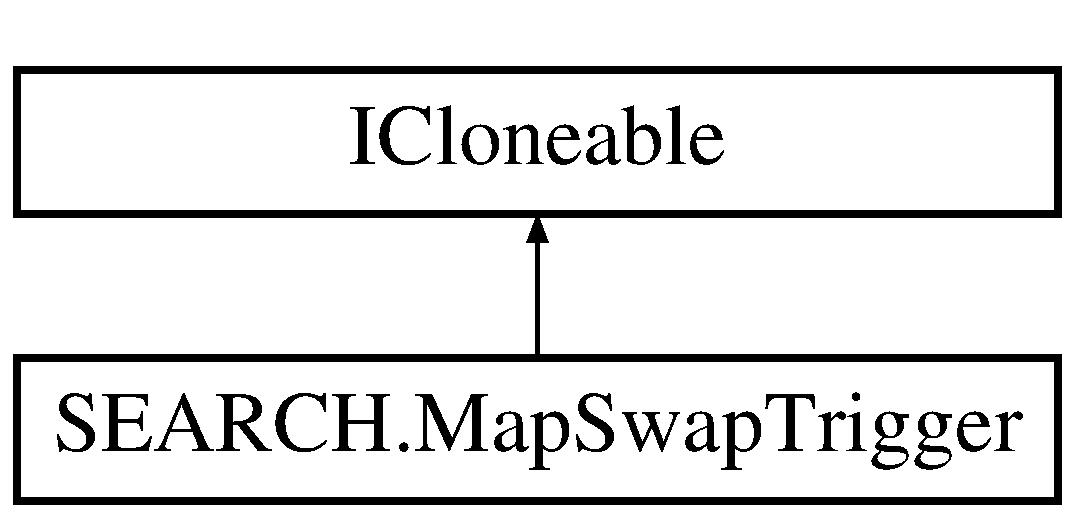
\includegraphics[height=2.000000cm]{class_s_e_a_r_c_h_1_1_map_swap_trigger}
\end{center}
\end{figure}
\subsection*{Public Types}
\begin{DoxyCompactItemize}
\item 
enum \hyperlink{class_s_e_a_r_c_h_1_1_map_swap_trigger_a293d493ac648d62dd39a2be6a8f7ff57}{m\-Trigger\-Type} \{ \hyperlink{class_s_e_a_r_c_h_1_1_map_swap_trigger_a293d493ac648d62dd39a2be6a8f7ff57afe6f99ef1ec99efbdc19a9786cf1facc}{S\-T\-A\-T\-I\-C}, 
\hyperlink{class_s_e_a_r_c_h_1_1_map_swap_trigger_a293d493ac648d62dd39a2be6a8f7ff57ae50d62d1ede0a4ea1acb310ff6ca4d5b}{Y\-E\-A\-R\-L\-Y}, 
\hyperlink{class_s_e_a_r_c_h_1_1_map_swap_trigger_a293d493ac648d62dd39a2be6a8f7ff57a791490f9f4842958f00f3791f6c01576}{D\-A\-I\-L\-Y}, 
\hyperlink{class_s_e_a_r_c_h_1_1_map_swap_trigger_a293d493ac648d62dd39a2be6a8f7ff57abaf6ff95d32557260caa379339315a4e}{H\-O\-U\-R\-L\-Y}
 \}
\end{DoxyCompactItemize}
\subsection*{Public Member Functions}
\begin{DoxyCompactItemize}
\item 
\hyperlink{class_s_e_a_r_c_h_1_1_map_swap_trigger_acd8315f88c4ef336b80e21b3143d7cdc}{Map\-Swap\-Trigger} ()
\item 
void \hyperlink{class_s_e_a_r_c_h_1_1_map_swap_trigger_a499d2fc210489af641d60e94715bf950}{set\-Trigger\-Type} (int num\-Years, int num\-Days, int num\-Hours)
\item 
override string \hyperlink{class_s_e_a_r_c_h_1_1_map_swap_trigger_ace21b377dca11a89c3639e286251a6d4}{To\-String} ()
\item 
object \hyperlink{class_s_e_a_r_c_h_1_1_map_swap_trigger_ad61079f6e7cb69f1ba72c036fe1be792}{Clone} ()
\end{DoxyCompactItemize}
\subsection*{Properties}
\begin{DoxyCompactItemize}
\item 
\hyperlink{class_s_e_a_r_c_h_1_1_map_swap_trigger_a293d493ac648d62dd39a2be6a8f7ff57}{m\-Trigger\-Type} \hyperlink{class_s_e_a_r_c_h_1_1_map_swap_trigger_ad78240ed34f35d77765b11ba553310cb}{My\-Trigger\-Type}\hspace{0.3cm}{\ttfamily  \mbox{[}get, set\mbox{]}}
\item 
int \hyperlink{class_s_e_a_r_c_h_1_1_map_swap_trigger_aeb5c52a1e6a860cad8f9c33e589d8f02}{Year\-Grp}\hspace{0.3cm}{\ttfamily  \mbox{[}get, set\mbox{]}}
\item 
int \hyperlink{class_s_e_a_r_c_h_1_1_map_swap_trigger_aab3ddb41ca60a79a37990b91e54eede4}{Season\-Grp}\hspace{0.3cm}{\ttfamily  \mbox{[}get, set\mbox{]}}
\item 
int \hyperlink{class_s_e_a_r_c_h_1_1_map_swap_trigger_aad1363d2548dd807ab35ab3201766ec7}{Day\-Grp}\hspace{0.3cm}{\ttfamily  \mbox{[}get, set\mbox{]}}
\item 
string \hyperlink{class_s_e_a_r_c_h_1_1_map_swap_trigger_a34aae23325a23e73fcac09220cd7ba34}{Start\-Month}\hspace{0.3cm}{\ttfamily  \mbox{[}get, set\mbox{]}}
\item 
string \hyperlink{class_s_e_a_r_c_h_1_1_map_swap_trigger_a9c72618cf0599bde747f74d6bdff0564}{Start\-Day}\hspace{0.3cm}{\ttfamily  \mbox{[}get, set\mbox{]}}
\item 
string \hyperlink{class_s_e_a_r_c_h_1_1_map_swap_trigger_abe8a3d6289f9b91f880c806c1513d23b}{Start\-Hour}\hspace{0.3cm}{\ttfamily  \mbox{[}get, set\mbox{]}}
\item 
string \hyperlink{class_s_e_a_r_c_h_1_1_map_swap_trigger_a48a4deb9d2e065b1490580f0296913e6}{Start\-Minute}\hspace{0.3cm}{\ttfamily  \mbox{[}get, set\mbox{]}}
\item 
System.\-Date\-Time \hyperlink{class_s_e_a_r_c_h_1_1_map_swap_trigger_a54e56a659c74906c32a4d52be8bdb13d}{Start\-Date}\hspace{0.3cm}{\ttfamily  \mbox{[}get, set\mbox{]}}
\item 
System.\-Date\-Time \hyperlink{class_s_e_a_r_c_h_1_1_map_swap_trigger_ada0854cccab56b3848a4f0c6ccabc200}{Original\-Start\-Date}\hspace{0.3cm}{\ttfamily  \mbox{[}get, set\mbox{]}}
\item 
string \hyperlink{class_s_e_a_r_c_h_1_1_map_swap_trigger_a1433599fc5a3a263d2076f1ea68c8cd1}{Path}\hspace{0.3cm}{\ttfamily  \mbox{[}get, set\mbox{]}}
\item 
string \hyperlink{class_s_e_a_r_c_h_1_1_map_swap_trigger_abc7b84ca520a70a857ef566eacfdb2a8}{Filename}\hspace{0.3cm}{\ttfamily  \mbox{[}get, set\mbox{]}}
\end{DoxyCompactItemize}


\subsection{Detailed Description}
Summary description for \hyperlink{class_s_e_a_r_c_h_1_1_map_swap_trigger}{Map\-Swap\-Trigger}. 



\subsection{Member Enumeration Documentation}
\hypertarget{class_s_e_a_r_c_h_1_1_map_swap_trigger_a293d493ac648d62dd39a2be6a8f7ff57}{\index{S\-E\-A\-R\-C\-H\-::\-Map\-Swap\-Trigger@{S\-E\-A\-R\-C\-H\-::\-Map\-Swap\-Trigger}!m\-Trigger\-Type@{m\-Trigger\-Type}}
\index{m\-Trigger\-Type@{m\-Trigger\-Type}!SEARCH::MapSwapTrigger@{S\-E\-A\-R\-C\-H\-::\-Map\-Swap\-Trigger}}
\subsubsection[{m\-Trigger\-Type}]{\setlength{\rightskip}{0pt plus 5cm}enum {\bf S\-E\-A\-R\-C\-H.\-Map\-Swap\-Trigger.\-m\-Trigger\-Type}}}\label{class_s_e_a_r_c_h_1_1_map_swap_trigger_a293d493ac648d62dd39a2be6a8f7ff57}
\begin{Desc}
\item[Enumerator]\par
\begin{description}
\index{S\-T\-A\-T\-I\-C@{S\-T\-A\-T\-I\-C}!S\-E\-A\-R\-C\-H\-::\-Map\-Swap\-Trigger@{S\-E\-A\-R\-C\-H\-::\-Map\-Swap\-Trigger}}\index{S\-E\-A\-R\-C\-H\-::\-Map\-Swap\-Trigger@{S\-E\-A\-R\-C\-H\-::\-Map\-Swap\-Trigger}!S\-T\-A\-T\-I\-C@{S\-T\-A\-T\-I\-C}}\item[{\em 
\hypertarget{class_s_e_a_r_c_h_1_1_map_swap_trigger_a293d493ac648d62dd39a2be6a8f7ff57afe6f99ef1ec99efbdc19a9786cf1facc}{S\-T\-A\-T\-I\-C}\label{class_s_e_a_r_c_h_1_1_map_swap_trigger_a293d493ac648d62dd39a2be6a8f7ff57afe6f99ef1ec99efbdc19a9786cf1facc}
}]\index{Y\-E\-A\-R\-L\-Y@{Y\-E\-A\-R\-L\-Y}!S\-E\-A\-R\-C\-H\-::\-Map\-Swap\-Trigger@{S\-E\-A\-R\-C\-H\-::\-Map\-Swap\-Trigger}}\index{S\-E\-A\-R\-C\-H\-::\-Map\-Swap\-Trigger@{S\-E\-A\-R\-C\-H\-::\-Map\-Swap\-Trigger}!Y\-E\-A\-R\-L\-Y@{Y\-E\-A\-R\-L\-Y}}\item[{\em 
\hypertarget{class_s_e_a_r_c_h_1_1_map_swap_trigger_a293d493ac648d62dd39a2be6a8f7ff57ae50d62d1ede0a4ea1acb310ff6ca4d5b}{Y\-E\-A\-R\-L\-Y}\label{class_s_e_a_r_c_h_1_1_map_swap_trigger_a293d493ac648d62dd39a2be6a8f7ff57ae50d62d1ede0a4ea1acb310ff6ca4d5b}
}]\index{D\-A\-I\-L\-Y@{D\-A\-I\-L\-Y}!S\-E\-A\-R\-C\-H\-::\-Map\-Swap\-Trigger@{S\-E\-A\-R\-C\-H\-::\-Map\-Swap\-Trigger}}\index{S\-E\-A\-R\-C\-H\-::\-Map\-Swap\-Trigger@{S\-E\-A\-R\-C\-H\-::\-Map\-Swap\-Trigger}!D\-A\-I\-L\-Y@{D\-A\-I\-L\-Y}}\item[{\em 
\hypertarget{class_s_e_a_r_c_h_1_1_map_swap_trigger_a293d493ac648d62dd39a2be6a8f7ff57a791490f9f4842958f00f3791f6c01576}{D\-A\-I\-L\-Y}\label{class_s_e_a_r_c_h_1_1_map_swap_trigger_a293d493ac648d62dd39a2be6a8f7ff57a791490f9f4842958f00f3791f6c01576}
}]\index{H\-O\-U\-R\-L\-Y@{H\-O\-U\-R\-L\-Y}!S\-E\-A\-R\-C\-H\-::\-Map\-Swap\-Trigger@{S\-E\-A\-R\-C\-H\-::\-Map\-Swap\-Trigger}}\index{S\-E\-A\-R\-C\-H\-::\-Map\-Swap\-Trigger@{S\-E\-A\-R\-C\-H\-::\-Map\-Swap\-Trigger}!H\-O\-U\-R\-L\-Y@{H\-O\-U\-R\-L\-Y}}\item[{\em 
\hypertarget{class_s_e_a_r_c_h_1_1_map_swap_trigger_a293d493ac648d62dd39a2be6a8f7ff57abaf6ff95d32557260caa379339315a4e}{H\-O\-U\-R\-L\-Y}\label{class_s_e_a_r_c_h_1_1_map_swap_trigger_a293d493ac648d62dd39a2be6a8f7ff57abaf6ff95d32557260caa379339315a4e}
}]\end{description}
\end{Desc}


\subsection{Constructor \& Destructor Documentation}
\hypertarget{class_s_e_a_r_c_h_1_1_map_swap_trigger_acd8315f88c4ef336b80e21b3143d7cdc}{\index{S\-E\-A\-R\-C\-H\-::\-Map\-Swap\-Trigger@{S\-E\-A\-R\-C\-H\-::\-Map\-Swap\-Trigger}!Map\-Swap\-Trigger@{Map\-Swap\-Trigger}}
\index{Map\-Swap\-Trigger@{Map\-Swap\-Trigger}!SEARCH::MapSwapTrigger@{S\-E\-A\-R\-C\-H\-::\-Map\-Swap\-Trigger}}
\subsubsection[{Map\-Swap\-Trigger}]{\setlength{\rightskip}{0pt plus 5cm}S\-E\-A\-R\-C\-H.\-Map\-Swap\-Trigger.\-Map\-Swap\-Trigger (
\begin{DoxyParamCaption}
{}
\end{DoxyParamCaption}
)}}\label{class_s_e_a_r_c_h_1_1_map_swap_trigger_acd8315f88c4ef336b80e21b3143d7cdc}


\subsection{Member Function Documentation}
\hypertarget{class_s_e_a_r_c_h_1_1_map_swap_trigger_ad61079f6e7cb69f1ba72c036fe1be792}{\index{S\-E\-A\-R\-C\-H\-::\-Map\-Swap\-Trigger@{S\-E\-A\-R\-C\-H\-::\-Map\-Swap\-Trigger}!Clone@{Clone}}
\index{Clone@{Clone}!SEARCH::MapSwapTrigger@{S\-E\-A\-R\-C\-H\-::\-Map\-Swap\-Trigger}}
\subsubsection[{Clone}]{\setlength{\rightskip}{0pt plus 5cm}object S\-E\-A\-R\-C\-H.\-Map\-Swap\-Trigger.\-Clone (
\begin{DoxyParamCaption}
{}
\end{DoxyParamCaption}
)}}\label{class_s_e_a_r_c_h_1_1_map_swap_trigger_ad61079f6e7cb69f1ba72c036fe1be792}
\hypertarget{class_s_e_a_r_c_h_1_1_map_swap_trigger_a499d2fc210489af641d60e94715bf950}{\index{S\-E\-A\-R\-C\-H\-::\-Map\-Swap\-Trigger@{S\-E\-A\-R\-C\-H\-::\-Map\-Swap\-Trigger}!set\-Trigger\-Type@{set\-Trigger\-Type}}
\index{set\-Trigger\-Type@{set\-Trigger\-Type}!SEARCH::MapSwapTrigger@{S\-E\-A\-R\-C\-H\-::\-Map\-Swap\-Trigger}}
\subsubsection[{set\-Trigger\-Type}]{\setlength{\rightskip}{0pt plus 5cm}void S\-E\-A\-R\-C\-H.\-Map\-Swap\-Trigger.\-set\-Trigger\-Type (
\begin{DoxyParamCaption}
\item[{int}]{num\-Years, }
\item[{int}]{num\-Days, }
\item[{int}]{num\-Hours}
\end{DoxyParamCaption}
)}}\label{class_s_e_a_r_c_h_1_1_map_swap_trigger_a499d2fc210489af641d60e94715bf950}
\hypertarget{class_s_e_a_r_c_h_1_1_map_swap_trigger_ace21b377dca11a89c3639e286251a6d4}{\index{S\-E\-A\-R\-C\-H\-::\-Map\-Swap\-Trigger@{S\-E\-A\-R\-C\-H\-::\-Map\-Swap\-Trigger}!To\-String@{To\-String}}
\index{To\-String@{To\-String}!SEARCH::MapSwapTrigger@{S\-E\-A\-R\-C\-H\-::\-Map\-Swap\-Trigger}}
\subsubsection[{To\-String}]{\setlength{\rightskip}{0pt plus 5cm}override string S\-E\-A\-R\-C\-H.\-Map\-Swap\-Trigger.\-To\-String (
\begin{DoxyParamCaption}
{}
\end{DoxyParamCaption}
)}}\label{class_s_e_a_r_c_h_1_1_map_swap_trigger_ace21b377dca11a89c3639e286251a6d4}


\subsection{Property Documentation}
\hypertarget{class_s_e_a_r_c_h_1_1_map_swap_trigger_aad1363d2548dd807ab35ab3201766ec7}{\index{S\-E\-A\-R\-C\-H\-::\-Map\-Swap\-Trigger@{S\-E\-A\-R\-C\-H\-::\-Map\-Swap\-Trigger}!Day\-Grp@{Day\-Grp}}
\index{Day\-Grp@{Day\-Grp}!SEARCH::MapSwapTrigger@{S\-E\-A\-R\-C\-H\-::\-Map\-Swap\-Trigger}}
\subsubsection[{Day\-Grp}]{\setlength{\rightskip}{0pt plus 5cm}int S\-E\-A\-R\-C\-H.\-Map\-Swap\-Trigger.\-Day\-Grp\hspace{0.3cm}{\ttfamily [get]}, {\ttfamily [set]}}}\label{class_s_e_a_r_c_h_1_1_map_swap_trigger_aad1363d2548dd807ab35ab3201766ec7}
\hypertarget{class_s_e_a_r_c_h_1_1_map_swap_trigger_abc7b84ca520a70a857ef566eacfdb2a8}{\index{S\-E\-A\-R\-C\-H\-::\-Map\-Swap\-Trigger@{S\-E\-A\-R\-C\-H\-::\-Map\-Swap\-Trigger}!Filename@{Filename}}
\index{Filename@{Filename}!SEARCH::MapSwapTrigger@{S\-E\-A\-R\-C\-H\-::\-Map\-Swap\-Trigger}}
\subsubsection[{Filename}]{\setlength{\rightskip}{0pt plus 5cm}string S\-E\-A\-R\-C\-H.\-Map\-Swap\-Trigger.\-Filename\hspace{0.3cm}{\ttfamily [get]}, {\ttfamily [set]}}}\label{class_s_e_a_r_c_h_1_1_map_swap_trigger_abc7b84ca520a70a857ef566eacfdb2a8}
\hypertarget{class_s_e_a_r_c_h_1_1_map_swap_trigger_ad78240ed34f35d77765b11ba553310cb}{\index{S\-E\-A\-R\-C\-H\-::\-Map\-Swap\-Trigger@{S\-E\-A\-R\-C\-H\-::\-Map\-Swap\-Trigger}!My\-Trigger\-Type@{My\-Trigger\-Type}}
\index{My\-Trigger\-Type@{My\-Trigger\-Type}!SEARCH::MapSwapTrigger@{S\-E\-A\-R\-C\-H\-::\-Map\-Swap\-Trigger}}
\subsubsection[{My\-Trigger\-Type}]{\setlength{\rightskip}{0pt plus 5cm}{\bf m\-Trigger\-Type} S\-E\-A\-R\-C\-H.\-Map\-Swap\-Trigger.\-My\-Trigger\-Type\hspace{0.3cm}{\ttfamily [get]}, {\ttfamily [set]}}}\label{class_s_e_a_r_c_h_1_1_map_swap_trigger_ad78240ed34f35d77765b11ba553310cb}
\hypertarget{class_s_e_a_r_c_h_1_1_map_swap_trigger_ada0854cccab56b3848a4f0c6ccabc200}{\index{S\-E\-A\-R\-C\-H\-::\-Map\-Swap\-Trigger@{S\-E\-A\-R\-C\-H\-::\-Map\-Swap\-Trigger}!Original\-Start\-Date@{Original\-Start\-Date}}
\index{Original\-Start\-Date@{Original\-Start\-Date}!SEARCH::MapSwapTrigger@{S\-E\-A\-R\-C\-H\-::\-Map\-Swap\-Trigger}}
\subsubsection[{Original\-Start\-Date}]{\setlength{\rightskip}{0pt plus 5cm}System.\-Date\-Time S\-E\-A\-R\-C\-H.\-Map\-Swap\-Trigger.\-Original\-Start\-Date\hspace{0.3cm}{\ttfamily [get]}, {\ttfamily [set]}}}\label{class_s_e_a_r_c_h_1_1_map_swap_trigger_ada0854cccab56b3848a4f0c6ccabc200}
\hypertarget{class_s_e_a_r_c_h_1_1_map_swap_trigger_a1433599fc5a3a263d2076f1ea68c8cd1}{\index{S\-E\-A\-R\-C\-H\-::\-Map\-Swap\-Trigger@{S\-E\-A\-R\-C\-H\-::\-Map\-Swap\-Trigger}!Path@{Path}}
\index{Path@{Path}!SEARCH::MapSwapTrigger@{S\-E\-A\-R\-C\-H\-::\-Map\-Swap\-Trigger}}
\subsubsection[{Path}]{\setlength{\rightskip}{0pt plus 5cm}string S\-E\-A\-R\-C\-H.\-Map\-Swap\-Trigger.\-Path\hspace{0.3cm}{\ttfamily [get]}, {\ttfamily [set]}}}\label{class_s_e_a_r_c_h_1_1_map_swap_trigger_a1433599fc5a3a263d2076f1ea68c8cd1}
\hypertarget{class_s_e_a_r_c_h_1_1_map_swap_trigger_aab3ddb41ca60a79a37990b91e54eede4}{\index{S\-E\-A\-R\-C\-H\-::\-Map\-Swap\-Trigger@{S\-E\-A\-R\-C\-H\-::\-Map\-Swap\-Trigger}!Season\-Grp@{Season\-Grp}}
\index{Season\-Grp@{Season\-Grp}!SEARCH::MapSwapTrigger@{S\-E\-A\-R\-C\-H\-::\-Map\-Swap\-Trigger}}
\subsubsection[{Season\-Grp}]{\setlength{\rightskip}{0pt plus 5cm}int S\-E\-A\-R\-C\-H.\-Map\-Swap\-Trigger.\-Season\-Grp\hspace{0.3cm}{\ttfamily [get]}, {\ttfamily [set]}}}\label{class_s_e_a_r_c_h_1_1_map_swap_trigger_aab3ddb41ca60a79a37990b91e54eede4}
\hypertarget{class_s_e_a_r_c_h_1_1_map_swap_trigger_a54e56a659c74906c32a4d52be8bdb13d}{\index{S\-E\-A\-R\-C\-H\-::\-Map\-Swap\-Trigger@{S\-E\-A\-R\-C\-H\-::\-Map\-Swap\-Trigger}!Start\-Date@{Start\-Date}}
\index{Start\-Date@{Start\-Date}!SEARCH::MapSwapTrigger@{S\-E\-A\-R\-C\-H\-::\-Map\-Swap\-Trigger}}
\subsubsection[{Start\-Date}]{\setlength{\rightskip}{0pt plus 5cm}System.\-Date\-Time S\-E\-A\-R\-C\-H.\-Map\-Swap\-Trigger.\-Start\-Date\hspace{0.3cm}{\ttfamily [get]}, {\ttfamily [set]}}}\label{class_s_e_a_r_c_h_1_1_map_swap_trigger_a54e56a659c74906c32a4d52be8bdb13d}
\hypertarget{class_s_e_a_r_c_h_1_1_map_swap_trigger_a9c72618cf0599bde747f74d6bdff0564}{\index{S\-E\-A\-R\-C\-H\-::\-Map\-Swap\-Trigger@{S\-E\-A\-R\-C\-H\-::\-Map\-Swap\-Trigger}!Start\-Day@{Start\-Day}}
\index{Start\-Day@{Start\-Day}!SEARCH::MapSwapTrigger@{S\-E\-A\-R\-C\-H\-::\-Map\-Swap\-Trigger}}
\subsubsection[{Start\-Day}]{\setlength{\rightskip}{0pt plus 5cm}string S\-E\-A\-R\-C\-H.\-Map\-Swap\-Trigger.\-Start\-Day\hspace{0.3cm}{\ttfamily [get]}, {\ttfamily [set]}}}\label{class_s_e_a_r_c_h_1_1_map_swap_trigger_a9c72618cf0599bde747f74d6bdff0564}
\hypertarget{class_s_e_a_r_c_h_1_1_map_swap_trigger_abe8a3d6289f9b91f880c806c1513d23b}{\index{S\-E\-A\-R\-C\-H\-::\-Map\-Swap\-Trigger@{S\-E\-A\-R\-C\-H\-::\-Map\-Swap\-Trigger}!Start\-Hour@{Start\-Hour}}
\index{Start\-Hour@{Start\-Hour}!SEARCH::MapSwapTrigger@{S\-E\-A\-R\-C\-H\-::\-Map\-Swap\-Trigger}}
\subsubsection[{Start\-Hour}]{\setlength{\rightskip}{0pt plus 5cm}string S\-E\-A\-R\-C\-H.\-Map\-Swap\-Trigger.\-Start\-Hour\hspace{0.3cm}{\ttfamily [get]}, {\ttfamily [set]}}}\label{class_s_e_a_r_c_h_1_1_map_swap_trigger_abe8a3d6289f9b91f880c806c1513d23b}
\hypertarget{class_s_e_a_r_c_h_1_1_map_swap_trigger_a48a4deb9d2e065b1490580f0296913e6}{\index{S\-E\-A\-R\-C\-H\-::\-Map\-Swap\-Trigger@{S\-E\-A\-R\-C\-H\-::\-Map\-Swap\-Trigger}!Start\-Minute@{Start\-Minute}}
\index{Start\-Minute@{Start\-Minute}!SEARCH::MapSwapTrigger@{S\-E\-A\-R\-C\-H\-::\-Map\-Swap\-Trigger}}
\subsubsection[{Start\-Minute}]{\setlength{\rightskip}{0pt plus 5cm}string S\-E\-A\-R\-C\-H.\-Map\-Swap\-Trigger.\-Start\-Minute\hspace{0.3cm}{\ttfamily [get]}, {\ttfamily [set]}}}\label{class_s_e_a_r_c_h_1_1_map_swap_trigger_a48a4deb9d2e065b1490580f0296913e6}
\hypertarget{class_s_e_a_r_c_h_1_1_map_swap_trigger_a34aae23325a23e73fcac09220cd7ba34}{\index{S\-E\-A\-R\-C\-H\-::\-Map\-Swap\-Trigger@{S\-E\-A\-R\-C\-H\-::\-Map\-Swap\-Trigger}!Start\-Month@{Start\-Month}}
\index{Start\-Month@{Start\-Month}!SEARCH::MapSwapTrigger@{S\-E\-A\-R\-C\-H\-::\-Map\-Swap\-Trigger}}
\subsubsection[{Start\-Month}]{\setlength{\rightskip}{0pt plus 5cm}string S\-E\-A\-R\-C\-H.\-Map\-Swap\-Trigger.\-Start\-Month\hspace{0.3cm}{\ttfamily [get]}, {\ttfamily [set]}}}\label{class_s_e_a_r_c_h_1_1_map_swap_trigger_a34aae23325a23e73fcac09220cd7ba34}
\hypertarget{class_s_e_a_r_c_h_1_1_map_swap_trigger_aeb5c52a1e6a860cad8f9c33e589d8f02}{\index{S\-E\-A\-R\-C\-H\-::\-Map\-Swap\-Trigger@{S\-E\-A\-R\-C\-H\-::\-Map\-Swap\-Trigger}!Year\-Grp@{Year\-Grp}}
\index{Year\-Grp@{Year\-Grp}!SEARCH::MapSwapTrigger@{S\-E\-A\-R\-C\-H\-::\-Map\-Swap\-Trigger}}
\subsubsection[{Year\-Grp}]{\setlength{\rightskip}{0pt plus 5cm}int S\-E\-A\-R\-C\-H.\-Map\-Swap\-Trigger.\-Year\-Grp\hspace{0.3cm}{\ttfamily [get]}, {\ttfamily [set]}}}\label{class_s_e_a_r_c_h_1_1_map_swap_trigger_aeb5c52a1e6a860cad8f9c33e589d8f02}


The documentation for this class was generated from the following file\-:\begin{DoxyCompactItemize}
\item 
Desktop/vlog4net\-A\-R\-C10\-\_\-64\-\_\-newhoming/\-Data\-Centric/\hyperlink{_map_swap_trigger_8cs}{Map\-Swap\-Trigger.\-cs}\end{DoxyCompactItemize}

\hypertarget{struct_s_e_a_r_c_h_1_1_map_value}{\section{S\-E\-A\-R\-C\-H.\-Map\-Value Struct Reference}
\label{struct_s_e_a_r_c_h_1_1_map_value}\index{S\-E\-A\-R\-C\-H.\-Map\-Value@{S\-E\-A\-R\-C\-H.\-Map\-Value}}
}
\subsection*{Properties}
\begin{DoxyCompactItemize}
\item 
double \hyperlink{struct_s_e_a_r_c_h_1_1_map_value_ac060f74c95e4074878b1bd9753c51e34}{Capture\-Food}\hspace{0.3cm}{\ttfamily  \mbox{[}get, set\mbox{]}}
\item 
I\-Point \hyperlink{struct_s_e_a_r_c_h_1_1_map_value_ac4ffd2c74d29fb17d41494ecac314c47}{Curr\-Location}\hspace{0.3cm}{\ttfamily  \mbox{[}get, set\mbox{]}}
\item 
double \hyperlink{struct_s_e_a_r_c_h_1_1_map_value_a517c6bbddd0e30a3c502ffffc3b34890}{Energy\-Used}\hspace{0.3cm}{\ttfamily  \mbox{[}get, set\mbox{]}}
\item 
int \hyperlink{struct_s_e_a_r_c_h_1_1_map_value_a76ef37bdb2e01254a40d643d6c9db2db}{Food\-Index}\hspace{0.3cm}{\ttfamily  \mbox{[}get, set\mbox{]}}
\item 
double \hyperlink{struct_s_e_a_r_c_h_1_1_map_value_a5da9e2d1378c114877a10bc2557a2d3d}{Food\-Mean\-Size}\hspace{0.3cm}{\ttfamily  \mbox{[}get, set\mbox{]}}
\item 
double \hyperlink{struct_s_e_a_r_c_h_1_1_map_value_a359ccb8e3bc9586205c978f44097e0cb}{Food\-S\-D\-\_\-\-Size}\hspace{0.3cm}{\ttfamily  \mbox{[}get, set\mbox{]}}
\item 
double \hyperlink{struct_s_e_a_r_c_h_1_1_map_value_a3a4afa7f6337324974e4755166c9f881}{Heading}\hspace{0.3cm}{\ttfamily  \mbox{[}get, set\mbox{]}}
\item 
int \hyperlink{struct_s_e_a_r_c_h_1_1_map_value_a2d19e4193ddf809036e9057a619ee789}{Move\-Index}\hspace{0.3cm}{\ttfamily  \mbox{[}get, set\mbox{]}}
\item 
double \hyperlink{struct_s_e_a_r_c_h_1_1_map_value_ac2b2fa609487c0a9c40145de61cc22e6}{Move\-Speed}\hspace{0.3cm}{\ttfamily  \mbox{[}get, set\mbox{]}}
\item 
double \hyperlink{struct_s_e_a_r_c_h_1_1_map_value_af99c02510a4a73fcce27364102b6ad47}{Move\-Turtosity}\hspace{0.3cm}{\ttfamily  \mbox{[}get, set\mbox{]}}
\item 
double \hyperlink{struct_s_e_a_r_c_h_1_1_map_value_a9a8251a69f96925a773d84678810744f}{Perception\-Dist}\hspace{0.3cm}{\ttfamily  \mbox{[}get, set\mbox{]}}
\item 
double \hyperlink{struct_s_e_a_r_c_h_1_1_map_value_a354901262d244a5caaa4e1cff659daee}{Percepton\-Modifier}\hspace{0.3cm}{\ttfamily  \mbox{[}get, set\mbox{]}}
\item 
double \hyperlink{struct_s_e_a_r_c_h_1_1_map_value_a7731481da862699355c683c2a980e960}{Predation\-Risk}\hspace{0.3cm}{\ttfamily  \mbox{[}get, set\mbox{]}}
\item 
int \hyperlink{struct_s_e_a_r_c_h_1_1_map_value_a740cf54c78bf4f868baab6ad3a590dd3}{Risk\-Index}\hspace{0.3cm}{\ttfamily  \mbox{[}get, set\mbox{]}}
\item 
int \hyperlink{struct_s_e_a_r_c_h_1_1_map_value_a30084a0a1fd7c7810984897e41ff1b44}{Social\-Index}\hspace{0.3cm}{\ttfamily  \mbox{[}get, set\mbox{]}}
\end{DoxyCompactItemize}


\subsection{Property Documentation}
\hypertarget{struct_s_e_a_r_c_h_1_1_map_value_ac060f74c95e4074878b1bd9753c51e34}{\index{S\-E\-A\-R\-C\-H\-::\-Map\-Value@{S\-E\-A\-R\-C\-H\-::\-Map\-Value}!Capture\-Food@{Capture\-Food}}
\index{Capture\-Food@{Capture\-Food}!SEARCH::MapValue@{S\-E\-A\-R\-C\-H\-::\-Map\-Value}}
\subsubsection[{Capture\-Food}]{\setlength{\rightskip}{0pt plus 5cm}double S\-E\-A\-R\-C\-H.\-Map\-Value.\-Capture\-Food\hspace{0.3cm}{\ttfamily [get]}, {\ttfamily [set]}}}\label{struct_s_e_a_r_c_h_1_1_map_value_ac060f74c95e4074878b1bd9753c51e34}
\hypertarget{struct_s_e_a_r_c_h_1_1_map_value_ac4ffd2c74d29fb17d41494ecac314c47}{\index{S\-E\-A\-R\-C\-H\-::\-Map\-Value@{S\-E\-A\-R\-C\-H\-::\-Map\-Value}!Curr\-Location@{Curr\-Location}}
\index{Curr\-Location@{Curr\-Location}!SEARCH::MapValue@{S\-E\-A\-R\-C\-H\-::\-Map\-Value}}
\subsubsection[{Curr\-Location}]{\setlength{\rightskip}{0pt plus 5cm}I\-Point S\-E\-A\-R\-C\-H.\-Map\-Value.\-Curr\-Location\hspace{0.3cm}{\ttfamily [get]}, {\ttfamily [set]}}}\label{struct_s_e_a_r_c_h_1_1_map_value_ac4ffd2c74d29fb17d41494ecac314c47}
\hypertarget{struct_s_e_a_r_c_h_1_1_map_value_a517c6bbddd0e30a3c502ffffc3b34890}{\index{S\-E\-A\-R\-C\-H\-::\-Map\-Value@{S\-E\-A\-R\-C\-H\-::\-Map\-Value}!Energy\-Used@{Energy\-Used}}
\index{Energy\-Used@{Energy\-Used}!SEARCH::MapValue@{S\-E\-A\-R\-C\-H\-::\-Map\-Value}}
\subsubsection[{Energy\-Used}]{\setlength{\rightskip}{0pt plus 5cm}double S\-E\-A\-R\-C\-H.\-Map\-Value.\-Energy\-Used\hspace{0.3cm}{\ttfamily [get]}, {\ttfamily [set]}}}\label{struct_s_e_a_r_c_h_1_1_map_value_a517c6bbddd0e30a3c502ffffc3b34890}
\hypertarget{struct_s_e_a_r_c_h_1_1_map_value_a76ef37bdb2e01254a40d643d6c9db2db}{\index{S\-E\-A\-R\-C\-H\-::\-Map\-Value@{S\-E\-A\-R\-C\-H\-::\-Map\-Value}!Food\-Index@{Food\-Index}}
\index{Food\-Index@{Food\-Index}!SEARCH::MapValue@{S\-E\-A\-R\-C\-H\-::\-Map\-Value}}
\subsubsection[{Food\-Index}]{\setlength{\rightskip}{0pt plus 5cm}int S\-E\-A\-R\-C\-H.\-Map\-Value.\-Food\-Index\hspace{0.3cm}{\ttfamily [get]}, {\ttfamily [set]}}}\label{struct_s_e_a_r_c_h_1_1_map_value_a76ef37bdb2e01254a40d643d6c9db2db}
\hypertarget{struct_s_e_a_r_c_h_1_1_map_value_a5da9e2d1378c114877a10bc2557a2d3d}{\index{S\-E\-A\-R\-C\-H\-::\-Map\-Value@{S\-E\-A\-R\-C\-H\-::\-Map\-Value}!Food\-Mean\-Size@{Food\-Mean\-Size}}
\index{Food\-Mean\-Size@{Food\-Mean\-Size}!SEARCH::MapValue@{S\-E\-A\-R\-C\-H\-::\-Map\-Value}}
\subsubsection[{Food\-Mean\-Size}]{\setlength{\rightskip}{0pt plus 5cm}double S\-E\-A\-R\-C\-H.\-Map\-Value.\-Food\-Mean\-Size\hspace{0.3cm}{\ttfamily [get]}, {\ttfamily [set]}}}\label{struct_s_e_a_r_c_h_1_1_map_value_a5da9e2d1378c114877a10bc2557a2d3d}
\hypertarget{struct_s_e_a_r_c_h_1_1_map_value_a359ccb8e3bc9586205c978f44097e0cb}{\index{S\-E\-A\-R\-C\-H\-::\-Map\-Value@{S\-E\-A\-R\-C\-H\-::\-Map\-Value}!Food\-S\-D\-\_\-\-Size@{Food\-S\-D\-\_\-\-Size}}
\index{Food\-S\-D\-\_\-\-Size@{Food\-S\-D\-\_\-\-Size}!SEARCH::MapValue@{S\-E\-A\-R\-C\-H\-::\-Map\-Value}}
\subsubsection[{Food\-S\-D\-\_\-\-Size}]{\setlength{\rightskip}{0pt plus 5cm}double S\-E\-A\-R\-C\-H.\-Map\-Value.\-Food\-S\-D\-\_\-\-Size\hspace{0.3cm}{\ttfamily [get]}, {\ttfamily [set]}}}\label{struct_s_e_a_r_c_h_1_1_map_value_a359ccb8e3bc9586205c978f44097e0cb}
\hypertarget{struct_s_e_a_r_c_h_1_1_map_value_a3a4afa7f6337324974e4755166c9f881}{\index{S\-E\-A\-R\-C\-H\-::\-Map\-Value@{S\-E\-A\-R\-C\-H\-::\-Map\-Value}!Heading@{Heading}}
\index{Heading@{Heading}!SEARCH::MapValue@{S\-E\-A\-R\-C\-H\-::\-Map\-Value}}
\subsubsection[{Heading}]{\setlength{\rightskip}{0pt plus 5cm}double S\-E\-A\-R\-C\-H.\-Map\-Value.\-Heading\hspace{0.3cm}{\ttfamily [get]}, {\ttfamily [set]}}}\label{struct_s_e_a_r_c_h_1_1_map_value_a3a4afa7f6337324974e4755166c9f881}
\hypertarget{struct_s_e_a_r_c_h_1_1_map_value_a2d19e4193ddf809036e9057a619ee789}{\index{S\-E\-A\-R\-C\-H\-::\-Map\-Value@{S\-E\-A\-R\-C\-H\-::\-Map\-Value}!Move\-Index@{Move\-Index}}
\index{Move\-Index@{Move\-Index}!SEARCH::MapValue@{S\-E\-A\-R\-C\-H\-::\-Map\-Value}}
\subsubsection[{Move\-Index}]{\setlength{\rightskip}{0pt plus 5cm}int S\-E\-A\-R\-C\-H.\-Map\-Value.\-Move\-Index\hspace{0.3cm}{\ttfamily [get]}, {\ttfamily [set]}}}\label{struct_s_e_a_r_c_h_1_1_map_value_a2d19e4193ddf809036e9057a619ee789}
\hypertarget{struct_s_e_a_r_c_h_1_1_map_value_ac2b2fa609487c0a9c40145de61cc22e6}{\index{S\-E\-A\-R\-C\-H\-::\-Map\-Value@{S\-E\-A\-R\-C\-H\-::\-Map\-Value}!Move\-Speed@{Move\-Speed}}
\index{Move\-Speed@{Move\-Speed}!SEARCH::MapValue@{S\-E\-A\-R\-C\-H\-::\-Map\-Value}}
\subsubsection[{Move\-Speed}]{\setlength{\rightskip}{0pt plus 5cm}double S\-E\-A\-R\-C\-H.\-Map\-Value.\-Move\-Speed\hspace{0.3cm}{\ttfamily [get]}, {\ttfamily [set]}}}\label{struct_s_e_a_r_c_h_1_1_map_value_ac2b2fa609487c0a9c40145de61cc22e6}
\hypertarget{struct_s_e_a_r_c_h_1_1_map_value_af99c02510a4a73fcce27364102b6ad47}{\index{S\-E\-A\-R\-C\-H\-::\-Map\-Value@{S\-E\-A\-R\-C\-H\-::\-Map\-Value}!Move\-Turtosity@{Move\-Turtosity}}
\index{Move\-Turtosity@{Move\-Turtosity}!SEARCH::MapValue@{S\-E\-A\-R\-C\-H\-::\-Map\-Value}}
\subsubsection[{Move\-Turtosity}]{\setlength{\rightskip}{0pt plus 5cm}double S\-E\-A\-R\-C\-H.\-Map\-Value.\-Move\-Turtosity\hspace{0.3cm}{\ttfamily [get]}, {\ttfamily [set]}}}\label{struct_s_e_a_r_c_h_1_1_map_value_af99c02510a4a73fcce27364102b6ad47}
\hypertarget{struct_s_e_a_r_c_h_1_1_map_value_a9a8251a69f96925a773d84678810744f}{\index{S\-E\-A\-R\-C\-H\-::\-Map\-Value@{S\-E\-A\-R\-C\-H\-::\-Map\-Value}!Perception\-Dist@{Perception\-Dist}}
\index{Perception\-Dist@{Perception\-Dist}!SEARCH::MapValue@{S\-E\-A\-R\-C\-H\-::\-Map\-Value}}
\subsubsection[{Perception\-Dist}]{\setlength{\rightskip}{0pt plus 5cm}double S\-E\-A\-R\-C\-H.\-Map\-Value.\-Perception\-Dist\hspace{0.3cm}{\ttfamily [get]}, {\ttfamily [set]}}}\label{struct_s_e_a_r_c_h_1_1_map_value_a9a8251a69f96925a773d84678810744f}
\hypertarget{struct_s_e_a_r_c_h_1_1_map_value_a354901262d244a5caaa4e1cff659daee}{\index{S\-E\-A\-R\-C\-H\-::\-Map\-Value@{S\-E\-A\-R\-C\-H\-::\-Map\-Value}!Percepton\-Modifier@{Percepton\-Modifier}}
\index{Percepton\-Modifier@{Percepton\-Modifier}!SEARCH::MapValue@{S\-E\-A\-R\-C\-H\-::\-Map\-Value}}
\subsubsection[{Percepton\-Modifier}]{\setlength{\rightskip}{0pt plus 5cm}double S\-E\-A\-R\-C\-H.\-Map\-Value.\-Percepton\-Modifier\hspace{0.3cm}{\ttfamily [get]}, {\ttfamily [set]}}}\label{struct_s_e_a_r_c_h_1_1_map_value_a354901262d244a5caaa4e1cff659daee}
\hypertarget{struct_s_e_a_r_c_h_1_1_map_value_a7731481da862699355c683c2a980e960}{\index{S\-E\-A\-R\-C\-H\-::\-Map\-Value@{S\-E\-A\-R\-C\-H\-::\-Map\-Value}!Predation\-Risk@{Predation\-Risk}}
\index{Predation\-Risk@{Predation\-Risk}!SEARCH::MapValue@{S\-E\-A\-R\-C\-H\-::\-Map\-Value}}
\subsubsection[{Predation\-Risk}]{\setlength{\rightskip}{0pt plus 5cm}double S\-E\-A\-R\-C\-H.\-Map\-Value.\-Predation\-Risk\hspace{0.3cm}{\ttfamily [get]}, {\ttfamily [set]}}}\label{struct_s_e_a_r_c_h_1_1_map_value_a7731481da862699355c683c2a980e960}
\hypertarget{struct_s_e_a_r_c_h_1_1_map_value_a740cf54c78bf4f868baab6ad3a590dd3}{\index{S\-E\-A\-R\-C\-H\-::\-Map\-Value@{S\-E\-A\-R\-C\-H\-::\-Map\-Value}!Risk\-Index@{Risk\-Index}}
\index{Risk\-Index@{Risk\-Index}!SEARCH::MapValue@{S\-E\-A\-R\-C\-H\-::\-Map\-Value}}
\subsubsection[{Risk\-Index}]{\setlength{\rightskip}{0pt plus 5cm}int S\-E\-A\-R\-C\-H.\-Map\-Value.\-Risk\-Index\hspace{0.3cm}{\ttfamily [get]}, {\ttfamily [set]}}}\label{struct_s_e_a_r_c_h_1_1_map_value_a740cf54c78bf4f868baab6ad3a590dd3}
\hypertarget{struct_s_e_a_r_c_h_1_1_map_value_a30084a0a1fd7c7810984897e41ff1b44}{\index{S\-E\-A\-R\-C\-H\-::\-Map\-Value@{S\-E\-A\-R\-C\-H\-::\-Map\-Value}!Social\-Index@{Social\-Index}}
\index{Social\-Index@{Social\-Index}!SEARCH::MapValue@{S\-E\-A\-R\-C\-H\-::\-Map\-Value}}
\subsubsection[{Social\-Index}]{\setlength{\rightskip}{0pt plus 5cm}int S\-E\-A\-R\-C\-H.\-Map\-Value.\-Social\-Index\hspace{0.3cm}{\ttfamily [get]}, {\ttfamily [set]}}}\label{struct_s_e_a_r_c_h_1_1_map_value_a30084a0a1fd7c7810984897e41ff1b44}


The documentation for this struct was generated from the following file\-:\begin{DoxyCompactItemize}
\item 
Desktop/vlog4net\-A\-R\-C10\-\_\-64\-\_\-newhoming/\-Data\-Centric/\hyperlink{_map_value_8cs}{Map\-Value.\-cs}\end{DoxyCompactItemize}

\hypertarget{class_s_e_a_r_c_h_1_1_memory_map}{\section{S\-E\-A\-R\-C\-H.\-Memory\-Map Class Reference}
\label{class_s_e_a_r_c_h_1_1_memory_map}\index{S\-E\-A\-R\-C\-H.\-Memory\-Map@{S\-E\-A\-R\-C\-H.\-Memory\-Map}}
}
Inheritance diagram for S\-E\-A\-R\-C\-H.\-Memory\-Map\-:\begin{figure}[H]
\begin{center}
\leavevmode
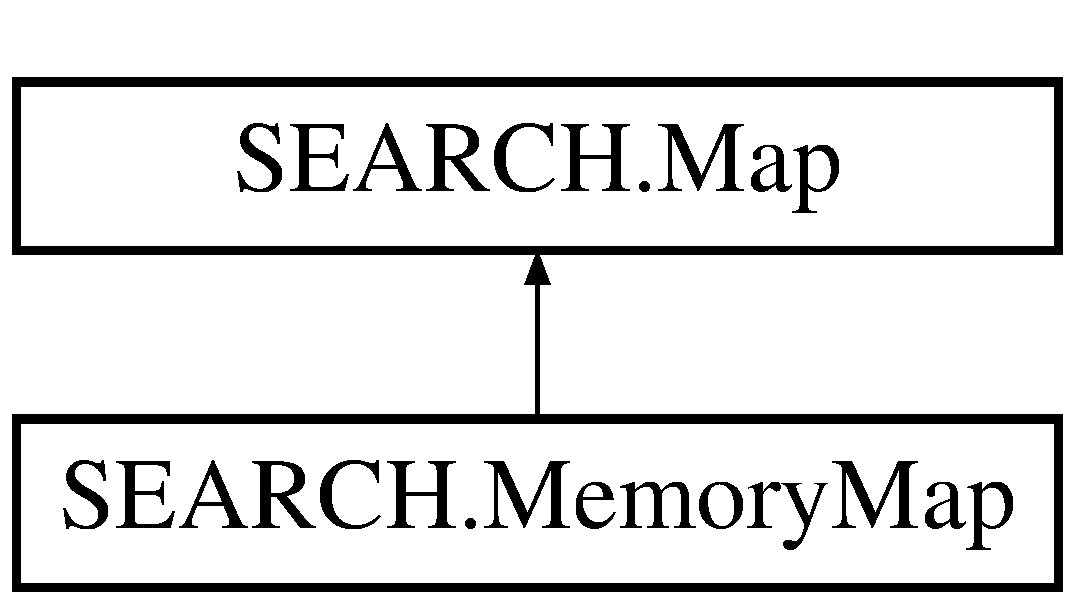
\includegraphics[height=2.000000cm]{class_s_e_a_r_c_h_1_1_memory_map}
\end{center}
\end{figure}
\subsection*{Public Member Functions}
\begin{DoxyCompactItemize}
\item 
\hyperlink{class_s_e_a_r_c_h_1_1_memory_map_a4a2426ab4a5ca0b2b9e59385edd8fb04}{Memory\-Map} (I\-Feature\-Class in\-Self)
\item 
new void \hyperlink{class_s_e_a_r_c_h_1_1_memory_map_af5ad1d8cea7ede46126b57bb405f2542}{Get\-Initial\-Animal\-Attributes} (out \hyperlink{class_s_e_a_r_c_h_1_1_initial_animal_attributes}{Initial\-Animal\-Attributes}\mbox{[}$\,$\mbox{]} out\-Attributes)
\begin{DoxyCompactList}\small\item\em When this map is first loaded we need to query the map and build the initial set of animals. this will return an array of Initial \hyperlink{class_s_e_a_r_c_h_1_1_animal}{Animal} Attributes. \end{DoxyCompactList}\end{DoxyCompactItemize}
\subsection*{Additional Inherited Members}


\subsection{Constructor \& Destructor Documentation}
\hypertarget{class_s_e_a_r_c_h_1_1_memory_map_a4a2426ab4a5ca0b2b9e59385edd8fb04}{\index{S\-E\-A\-R\-C\-H\-::\-Memory\-Map@{S\-E\-A\-R\-C\-H\-::\-Memory\-Map}!Memory\-Map@{Memory\-Map}}
\index{Memory\-Map@{Memory\-Map}!SEARCH::MemoryMap@{S\-E\-A\-R\-C\-H\-::\-Memory\-Map}}
\subsubsection[{Memory\-Map}]{\setlength{\rightskip}{0pt plus 5cm}S\-E\-A\-R\-C\-H.\-Memory\-Map.\-Memory\-Map (
\begin{DoxyParamCaption}
\item[{I\-Feature\-Class}]{in\-Self}
\end{DoxyParamCaption}
)}}\label{class_s_e_a_r_c_h_1_1_memory_map_a4a2426ab4a5ca0b2b9e59385edd8fb04}


\subsection{Member Function Documentation}
\hypertarget{class_s_e_a_r_c_h_1_1_memory_map_af5ad1d8cea7ede46126b57bb405f2542}{\index{S\-E\-A\-R\-C\-H\-::\-Memory\-Map@{S\-E\-A\-R\-C\-H\-::\-Memory\-Map}!Get\-Initial\-Animal\-Attributes@{Get\-Initial\-Animal\-Attributes}}
\index{Get\-Initial\-Animal\-Attributes@{Get\-Initial\-Animal\-Attributes}!SEARCH::MemoryMap@{S\-E\-A\-R\-C\-H\-::\-Memory\-Map}}
\subsubsection[{Get\-Initial\-Animal\-Attributes}]{\setlength{\rightskip}{0pt plus 5cm}new void S\-E\-A\-R\-C\-H.\-Memory\-Map.\-Get\-Initial\-Animal\-Attributes (
\begin{DoxyParamCaption}
\item[{out {\bf Initial\-Animal\-Attributes}\mbox{[}$\,$\mbox{]}}]{out\-Attributes}
\end{DoxyParamCaption}
)}}\label{class_s_e_a_r_c_h_1_1_memory_map_af5ad1d8cea7ede46126b57bb405f2542}


When this map is first loaded we need to query the map and build the initial set of animals. this will return an array of Initial \hyperlink{class_s_e_a_r_c_h_1_1_animal}{Animal} Attributes. 



The documentation for this class was generated from the following file\-:\begin{DoxyCompactItemize}
\item 
Desktop/vlog4net\-A\-R\-C10\-\_\-64\-\_\-newhoming/\-Data\-Centric/\hyperlink{_memory_map_8cs}{Memory\-Map.\-cs}\end{DoxyCompactItemize}

\hypertarget{class_s_e_a_r_c_h_1_1_modifier}{\section{S\-E\-A\-R\-C\-H.\-Modifier Class Reference}
\label{class_s_e_a_r_c_h_1_1_modifier}\index{S\-E\-A\-R\-C\-H.\-Modifier@{S\-E\-A\-R\-C\-H.\-Modifier}}
}
Inheritance diagram for S\-E\-A\-R\-C\-H.\-Modifier\-:\begin{figure}[H]
\begin{center}
\leavevmode
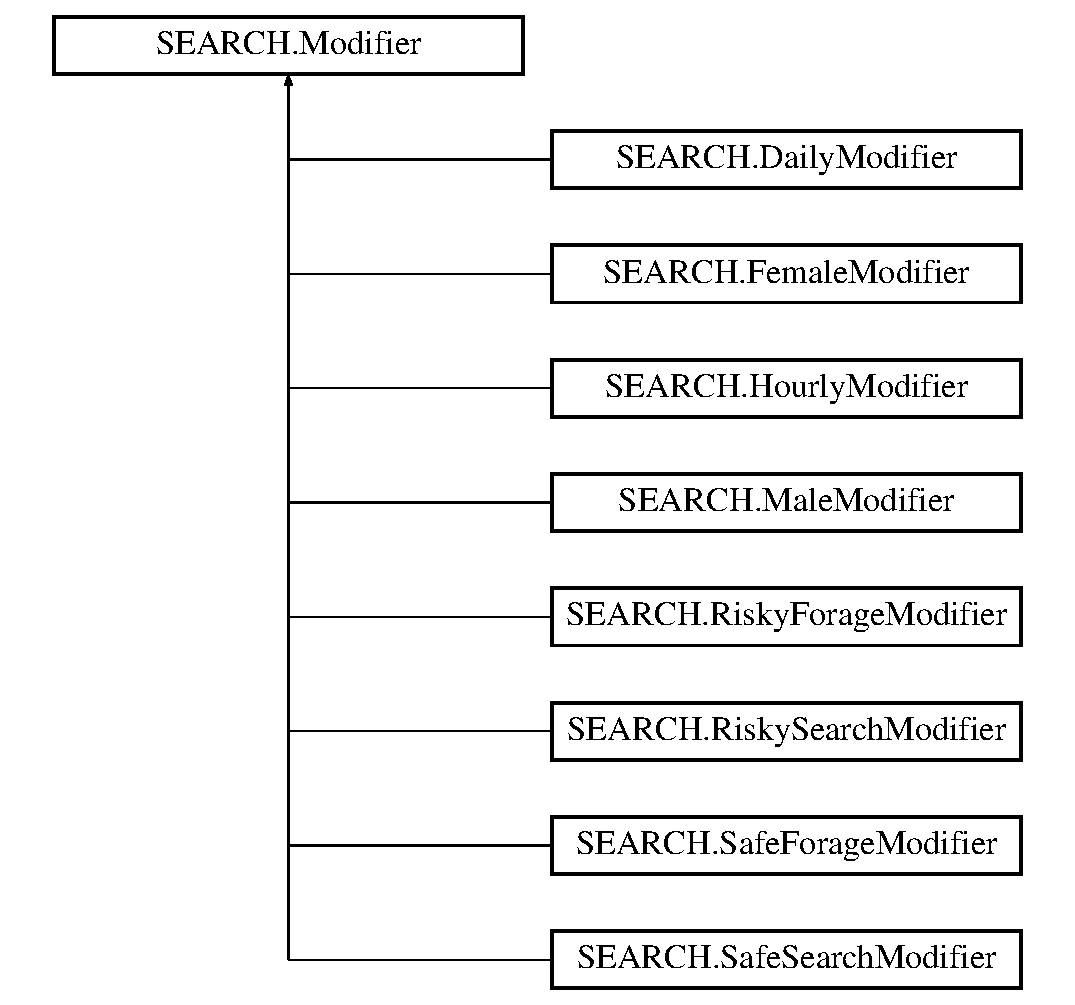
\includegraphics[height=9.000000cm]{class_s_e_a_r_c_h_1_1_modifier}
\end{center}
\end{figure}
\subsection*{Public Member Functions}
\begin{DoxyCompactItemize}
\item 
\hyperlink{class_s_e_a_r_c_h_1_1_modifier_a503804f862a61bd58e98945612fc276f}{Modifier} ()
\end{DoxyCompactItemize}
\subsection*{Properties}
\begin{DoxyCompactItemize}
\item 
string \hyperlink{class_s_e_a_r_c_h_1_1_modifier_ab012caf0cb9046e861692569acf540fd}{Name}\hspace{0.3cm}{\ttfamily  \mbox{[}get, set\mbox{]}}
\item 
double \hyperlink{class_s_e_a_r_c_h_1_1_modifier_ab5da9e34923a3d6b1df4e017ccb375e0}{Capture\-Food}\hspace{0.3cm}{\ttfamily  \mbox{[}get, set\mbox{]}}
\item 
double \hyperlink{class_s_e_a_r_c_h_1_1_modifier_ae62b3e7d070587389037bfa82a06a57c}{Predation\-Risk}\hspace{0.3cm}{\ttfamily  \mbox{[}get, set\mbox{]}}
\item 
double \hyperlink{class_s_e_a_r_c_h_1_1_modifier_aecfd3655abc64cc9f8d5bd15fce65032}{Move\-Speed}\hspace{0.3cm}{\ttfamily  \mbox{[}get, set\mbox{]}}
\item 
double \hyperlink{class_s_e_a_r_c_h_1_1_modifier_a8a5ec2af78ff48e8a69ce97ffc654e70}{Move\-Turtosity}\hspace{0.3cm}{\ttfamily  \mbox{[}get, set\mbox{]}}
\item 
double \hyperlink{class_s_e_a_r_c_h_1_1_modifier_ab65634462ad6c6e0b8c6e4702af1c477}{Energy\-Used}\hspace{0.3cm}{\ttfamily  \mbox{[}get, set\mbox{]}}
\item 
double \hyperlink{class_s_e_a_r_c_h_1_1_modifier_afae7871e75792196f3129ecbd9dc41d2}{Percepton\-Modifier}\hspace{0.3cm}{\ttfamily  \mbox{[}get, set\mbox{]}}
\end{DoxyCompactItemize}


\subsection{Constructor \& Destructor Documentation}
\hypertarget{class_s_e_a_r_c_h_1_1_modifier_a503804f862a61bd58e98945612fc276f}{\index{S\-E\-A\-R\-C\-H\-::\-Modifier@{S\-E\-A\-R\-C\-H\-::\-Modifier}!Modifier@{Modifier}}
\index{Modifier@{Modifier}!SEARCH::Modifier@{S\-E\-A\-R\-C\-H\-::\-Modifier}}
\subsubsection[{Modifier}]{\setlength{\rightskip}{0pt plus 5cm}S\-E\-A\-R\-C\-H.\-Modifier.\-Modifier (
\begin{DoxyParamCaption}
{}
\end{DoxyParamCaption}
)}}\label{class_s_e_a_r_c_h_1_1_modifier_a503804f862a61bd58e98945612fc276f}


\subsection{Property Documentation}
\hypertarget{class_s_e_a_r_c_h_1_1_modifier_ab5da9e34923a3d6b1df4e017ccb375e0}{\index{S\-E\-A\-R\-C\-H\-::\-Modifier@{S\-E\-A\-R\-C\-H\-::\-Modifier}!Capture\-Food@{Capture\-Food}}
\index{Capture\-Food@{Capture\-Food}!SEARCH::Modifier@{S\-E\-A\-R\-C\-H\-::\-Modifier}}
\subsubsection[{Capture\-Food}]{\setlength{\rightskip}{0pt plus 5cm}double S\-E\-A\-R\-C\-H.\-Modifier.\-Capture\-Food\hspace{0.3cm}{\ttfamily [get]}, {\ttfamily [set]}}}\label{class_s_e_a_r_c_h_1_1_modifier_ab5da9e34923a3d6b1df4e017ccb375e0}
\hypertarget{class_s_e_a_r_c_h_1_1_modifier_ab65634462ad6c6e0b8c6e4702af1c477}{\index{S\-E\-A\-R\-C\-H\-::\-Modifier@{S\-E\-A\-R\-C\-H\-::\-Modifier}!Energy\-Used@{Energy\-Used}}
\index{Energy\-Used@{Energy\-Used}!SEARCH::Modifier@{S\-E\-A\-R\-C\-H\-::\-Modifier}}
\subsubsection[{Energy\-Used}]{\setlength{\rightskip}{0pt plus 5cm}double S\-E\-A\-R\-C\-H.\-Modifier.\-Energy\-Used\hspace{0.3cm}{\ttfamily [get]}, {\ttfamily [set]}}}\label{class_s_e_a_r_c_h_1_1_modifier_ab65634462ad6c6e0b8c6e4702af1c477}
\hypertarget{class_s_e_a_r_c_h_1_1_modifier_aecfd3655abc64cc9f8d5bd15fce65032}{\index{S\-E\-A\-R\-C\-H\-::\-Modifier@{S\-E\-A\-R\-C\-H\-::\-Modifier}!Move\-Speed@{Move\-Speed}}
\index{Move\-Speed@{Move\-Speed}!SEARCH::Modifier@{S\-E\-A\-R\-C\-H\-::\-Modifier}}
\subsubsection[{Move\-Speed}]{\setlength{\rightskip}{0pt plus 5cm}double S\-E\-A\-R\-C\-H.\-Modifier.\-Move\-Speed\hspace{0.3cm}{\ttfamily [get]}, {\ttfamily [set]}}}\label{class_s_e_a_r_c_h_1_1_modifier_aecfd3655abc64cc9f8d5bd15fce65032}
\hypertarget{class_s_e_a_r_c_h_1_1_modifier_a8a5ec2af78ff48e8a69ce97ffc654e70}{\index{S\-E\-A\-R\-C\-H\-::\-Modifier@{S\-E\-A\-R\-C\-H\-::\-Modifier}!Move\-Turtosity@{Move\-Turtosity}}
\index{Move\-Turtosity@{Move\-Turtosity}!SEARCH::Modifier@{S\-E\-A\-R\-C\-H\-::\-Modifier}}
\subsubsection[{Move\-Turtosity}]{\setlength{\rightskip}{0pt plus 5cm}double S\-E\-A\-R\-C\-H.\-Modifier.\-Move\-Turtosity\hspace{0.3cm}{\ttfamily [get]}, {\ttfamily [set]}}}\label{class_s_e_a_r_c_h_1_1_modifier_a8a5ec2af78ff48e8a69ce97ffc654e70}
\hypertarget{class_s_e_a_r_c_h_1_1_modifier_ab012caf0cb9046e861692569acf540fd}{\index{S\-E\-A\-R\-C\-H\-::\-Modifier@{S\-E\-A\-R\-C\-H\-::\-Modifier}!Name@{Name}}
\index{Name@{Name}!SEARCH::Modifier@{S\-E\-A\-R\-C\-H\-::\-Modifier}}
\subsubsection[{Name}]{\setlength{\rightskip}{0pt plus 5cm}string S\-E\-A\-R\-C\-H.\-Modifier.\-Name\hspace{0.3cm}{\ttfamily [get]}, {\ttfamily [set]}}}\label{class_s_e_a_r_c_h_1_1_modifier_ab012caf0cb9046e861692569acf540fd}
\hypertarget{class_s_e_a_r_c_h_1_1_modifier_afae7871e75792196f3129ecbd9dc41d2}{\index{S\-E\-A\-R\-C\-H\-::\-Modifier@{S\-E\-A\-R\-C\-H\-::\-Modifier}!Percepton\-Modifier@{Percepton\-Modifier}}
\index{Percepton\-Modifier@{Percepton\-Modifier}!SEARCH::Modifier@{S\-E\-A\-R\-C\-H\-::\-Modifier}}
\subsubsection[{Percepton\-Modifier}]{\setlength{\rightskip}{0pt plus 5cm}double S\-E\-A\-R\-C\-H.\-Modifier.\-Percepton\-Modifier\hspace{0.3cm}{\ttfamily [get]}, {\ttfamily [set]}}}\label{class_s_e_a_r_c_h_1_1_modifier_afae7871e75792196f3129ecbd9dc41d2}
\hypertarget{class_s_e_a_r_c_h_1_1_modifier_ae62b3e7d070587389037bfa82a06a57c}{\index{S\-E\-A\-R\-C\-H\-::\-Modifier@{S\-E\-A\-R\-C\-H\-::\-Modifier}!Predation\-Risk@{Predation\-Risk}}
\index{Predation\-Risk@{Predation\-Risk}!SEARCH::Modifier@{S\-E\-A\-R\-C\-H\-::\-Modifier}}
\subsubsection[{Predation\-Risk}]{\setlength{\rightskip}{0pt plus 5cm}double S\-E\-A\-R\-C\-H.\-Modifier.\-Predation\-Risk\hspace{0.3cm}{\ttfamily [get]}, {\ttfamily [set]}}}\label{class_s_e_a_r_c_h_1_1_modifier_ae62b3e7d070587389037bfa82a06a57c}


The documentation for this class was generated from the following file\-:\begin{DoxyCompactItemize}
\item 
Desktop/vlog4net\-A\-R\-C10\-\_\-64\-\_\-newhoming/\-Data\-Centric/\hyperlink{_modifier_8cs}{Modifier.\-cs}\end{DoxyCompactItemize}

\hypertarget{class_s_e_a_r_c_h_1_1_mover}{\section{S\-E\-A\-R\-C\-H.\-Mover Class Reference}
\label{class_s_e_a_r_c_h_1_1_mover}\index{S\-E\-A\-R\-C\-H.\-Mover@{S\-E\-A\-R\-C\-H.\-Mover}}
}


Summary description for \hyperlink{class_s_e_a_r_c_h_1_1_mover}{Mover}.  


Inheritance diagram for S\-E\-A\-R\-C\-H.\-Mover\-:\begin{figure}[H]
\begin{center}
\leavevmode
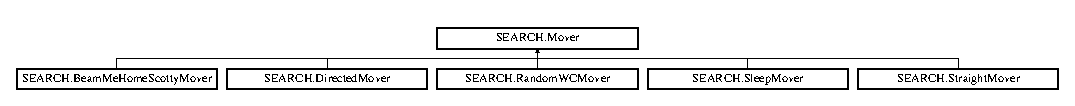
\includegraphics[height=0.982456cm]{class_s_e_a_r_c_h_1_1_mover}
\end{center}
\end{figure}
\subsection*{Public Member Functions}
\begin{DoxyCompactItemize}
\item 
\hyperlink{class_s_e_a_r_c_h_1_1_mover_aafc7e67b5b0bd68f9cfec99f68d76309}{Mover} ()
\item 
\hyperlink{class_s_e_a_r_c_h_1_1_mover_ac79713250c11901b081e460f3a0aef0c}{Mover} (System.\-Collections.\-Array\-List in\-Path)
\item 
\hyperlink{class_s_e_a_r_c_h_1_1_mover_a05f02fd5a8ba930d331210167c8268a0}{Mover} (System.\-Collections.\-Array\-List in\-Path, double in\-Base\-Step\-Length, double in\-Heading, double in\-Turn\-Angle\-Variability)
\item 
virtual void \hyperlink{class_s_e_a_r_c_h_1_1_mover_ab2dfc659f3817ea48d66ff4d7e464d1d}{move} (ref double percent\-Time\-Step, \hyperlink{class_s_e_a_r_c_h_1_1_animal}{Animal} in\-A)
\item 
abstract double \hyperlink{class_s_e_a_r_c_h_1_1_mover_a879a44d5a0c57434375a69c8d8d00e35}{get\-Turn\-Angle} (double turtosity)
\item 
abstract double \hyperlink{class_s_e_a_r_c_h_1_1_mover_a3e547800bbc34492f4251adee70dbf02}{get\-Step\-Length} ()
\item 
Point\-Class \hyperlink{class_s_e_a_r_c_h_1_1_mover_ae1603ac731e59e6b4ffc485e5b81e846}{step\-Back} (\hyperlink{class_s_e_a_r_c_h_1_1_animal}{Animal} in\-A)
\end{DoxyCompactItemize}
\subsection*{Static Public Member Functions}
\begin{DoxyCompactItemize}
\item 
static Point\-Class \hyperlink{class_s_e_a_r_c_h_1_1_mover_a0f3de12a1d5f59f098be3220d98ebd62}{step\-Forward} (I\-Point start\-Point, I\-Point end\-Point)
\item 
static void \hyperlink{class_s_e_a_r_c_h_1_1_mover_a360265c7744b22b0dc484135b6b77dad}{step\-Forward} (ref \hyperlink{class_s_e_a_r_c_h_1_1_animal}{Animal} in\-A)
\item 
static Point\-Class \hyperlink{class_s_e_a_r_c_h_1_1_mover_a84c8c83bb560d911cb9681ff32b93383}{step\-Back} (I\-Point start\-Point, I\-Point end\-Point)
\item 
static string \hyperlink{class_s_e_a_r_c_h_1_1_mover_a69c5168d8551e5c51893a9cbea9c93d4}{Point\-To\-String} (I\-Point in\-Point)
\end{DoxyCompactItemize}
\subsection*{Protected Attributes}
\begin{DoxyCompactItemize}
\item 
\hyperlink{class_s_e_a_r_c_h_1_1_map_manager}{Map\-Manager} \hyperlink{class_s_e_a_r_c_h_1_1_mover_a6ea0ee67a11b4bfe8802ff096c53e908}{my\-Map\-Manager}
\end{DoxyCompactItemize}
\subsection*{Properties}
\begin{DoxyCompactItemize}
\item 
System.\-Collections.\-Array\-List \hyperlink{class_s_e_a_r_c_h_1_1_mover_aaf46431549d9887e3710f2831cd906db}{Path}\hspace{0.3cm}{\ttfamily  \mbox{[}get, set\mbox{]}}
\item 
double \hyperlink{class_s_e_a_r_c_h_1_1_mover_aee1e8a76587d4b51e7db5b475b86ac97}{base\-Step\-Length}\hspace{0.3cm}{\ttfamily  \mbox{[}get, set\mbox{]}}
\begin{DoxyCompactList}\small\item\em This property represent the step length of any object that has a movement state. It is used by the \hyperlink{class_s_e_a_r_c_h_1_1_mover_ab2dfc659f3817ea48d66ff4d7e464d1d}{move()} method to determine the distance traveled during a particular time step. \end{DoxyCompactList}\item 
\hyperlink{class_s_e_a_r_c_h_1_1_point}{Point} \hyperlink{class_s_e_a_r_c_h_1_1_mover_adbd8f2d23d7a01350e2d598b15a0447d}{current\-Location}\hspace{0.3cm}{\ttfamily  \mbox{[}get, set\mbox{]}}
\item 
double \hyperlink{class_s_e_a_r_c_h_1_1_mover_a460b88ef4c0b1be0b4dfb20bb7d8cc6c}{heading}\hspace{0.3cm}{\ttfamily  \mbox{[}get, set\mbox{]}}
\begin{DoxyCompactList}\small\item\em This property represent the heading of any object that has a movement state. It is used by the \hyperlink{class_s_e_a_r_c_h_1_1_mover_ab2dfc659f3817ea48d66ff4d7e464d1d}{move()} method to determine the distance traveled during a particular time step. \end{DoxyCompactList}\item 
double \hyperlink{class_s_e_a_r_c_h_1_1_mover_ad26237e095a0ed3f40e097c699a22310}{turn\-Angle\-Variability}\hspace{0.3cm}{\ttfamily  \mbox{[}get, set\mbox{]}}
\begin{DoxyCompactList}\small\item\em This property is used by the random turn angle function to specify the degree of variation in the returned turn angle. \end{DoxyCompactList}\item 
double \hyperlink{class_s_e_a_r_c_h_1_1_mover_a09fda49c5f301e043fbe3fee2e5bf2eb}{terrain\-Step\-Modifier}\hspace{0.3cm}{\ttfamily  \mbox{[}get, set\mbox{]}}
\item 
double \hyperlink{class_s_e_a_r_c_h_1_1_mover_a1fb4ef0de58f74cdda8ba9487b4fe78c}{time\-Day\-Angle\-Modifier}\hspace{0.3cm}{\ttfamily  \mbox{[}get, set\mbox{]}}
\item 
double \hyperlink{class_s_e_a_r_c_h_1_1_mover_a64d50790add5dc402d87727fc149b8ee}{terrain\-Angle\-Modifier}\hspace{0.3cm}{\ttfamily  \mbox{[}get, set\mbox{]}}
\item 
double \hyperlink{class_s_e_a_r_c_h_1_1_mover_a7aea3c84939c22c9936941d025db6221}{time\-Day\-Step\-Modifier}\hspace{0.3cm}{\ttfamily  \mbox{[}get, set\mbox{]}}
\item 
double \hyperlink{class_s_e_a_r_c_h_1_1_mover_ad3fbdb8aa27d97c46638cbf5cb80ed2e}{time\-Year\-Step\-Modifier}\hspace{0.3cm}{\ttfamily  \mbox{[}get, set\mbox{]}}
\item 
double \hyperlink{class_s_e_a_r_c_h_1_1_mover_a73145c64b8c7be641c632dca87dc492d}{time\-Year\-Angle\-Modifier}\hspace{0.3cm}{\ttfamily  \mbox{[}get, set\mbox{]}}
\end{DoxyCompactItemize}


\subsection{Detailed Description}
Summary description for \hyperlink{class_s_e_a_r_c_h_1_1_mover}{Mover}. 



\subsection{Constructor \& Destructor Documentation}
\hypertarget{class_s_e_a_r_c_h_1_1_mover_aafc7e67b5b0bd68f9cfec99f68d76309}{\index{S\-E\-A\-R\-C\-H\-::\-Mover@{S\-E\-A\-R\-C\-H\-::\-Mover}!Mover@{Mover}}
\index{Mover@{Mover}!SEARCH::Mover@{S\-E\-A\-R\-C\-H\-::\-Mover}}
\subsubsection[{Mover}]{\setlength{\rightskip}{0pt plus 5cm}S\-E\-A\-R\-C\-H.\-Mover.\-Mover (
\begin{DoxyParamCaption}
{}
\end{DoxyParamCaption}
)}}\label{class_s_e_a_r_c_h_1_1_mover_aafc7e67b5b0bd68f9cfec99f68d76309}
\hypertarget{class_s_e_a_r_c_h_1_1_mover_ac79713250c11901b081e460f3a0aef0c}{\index{S\-E\-A\-R\-C\-H\-::\-Mover@{S\-E\-A\-R\-C\-H\-::\-Mover}!Mover@{Mover}}
\index{Mover@{Mover}!SEARCH::Mover@{S\-E\-A\-R\-C\-H\-::\-Mover}}
\subsubsection[{Mover}]{\setlength{\rightskip}{0pt plus 5cm}S\-E\-A\-R\-C\-H.\-Mover.\-Mover (
\begin{DoxyParamCaption}
\item[{System.\-Collections.\-Array\-List}]{in\-Path}
\end{DoxyParamCaption}
)}}\label{class_s_e_a_r_c_h_1_1_mover_ac79713250c11901b081e460f3a0aef0c}
\hypertarget{class_s_e_a_r_c_h_1_1_mover_a05f02fd5a8ba930d331210167c8268a0}{\index{S\-E\-A\-R\-C\-H\-::\-Mover@{S\-E\-A\-R\-C\-H\-::\-Mover}!Mover@{Mover}}
\index{Mover@{Mover}!SEARCH::Mover@{S\-E\-A\-R\-C\-H\-::\-Mover}}
\subsubsection[{Mover}]{\setlength{\rightskip}{0pt plus 5cm}S\-E\-A\-R\-C\-H.\-Mover.\-Mover (
\begin{DoxyParamCaption}
\item[{System.\-Collections.\-Array\-List}]{in\-Path, }
\item[{double}]{in\-Base\-Step\-Length, }
\item[{double}]{in\-Heading, }
\item[{double}]{in\-Turn\-Angle\-Variability}
\end{DoxyParamCaption}
)}}\label{class_s_e_a_r_c_h_1_1_mover_a05f02fd5a8ba930d331210167c8268a0}


\subsection{Member Function Documentation}
\hypertarget{class_s_e_a_r_c_h_1_1_mover_a3e547800bbc34492f4251adee70dbf02}{\index{S\-E\-A\-R\-C\-H\-::\-Mover@{S\-E\-A\-R\-C\-H\-::\-Mover}!get\-Step\-Length@{get\-Step\-Length}}
\index{get\-Step\-Length@{get\-Step\-Length}!SEARCH::Mover@{S\-E\-A\-R\-C\-H\-::\-Mover}}
\subsubsection[{get\-Step\-Length}]{\setlength{\rightskip}{0pt plus 5cm}abstract double S\-E\-A\-R\-C\-H.\-Mover.\-get\-Step\-Length (
\begin{DoxyParamCaption}
{}
\end{DoxyParamCaption}
)\hspace{0.3cm}{\ttfamily [pure virtual]}}}\label{class_s_e_a_r_c_h_1_1_mover_a3e547800bbc34492f4251adee70dbf02}


Implemented in \hyperlink{class_s_e_a_r_c_h_1_1_random_w_c_mover_a50f9ef5586b7740beeeb197b7334a560}{S\-E\-A\-R\-C\-H.\-Random\-W\-C\-Mover}, \hyperlink{class_s_e_a_r_c_h_1_1_sleep_mover_a00e109927daf570d0c406339478131f9}{S\-E\-A\-R\-C\-H.\-Sleep\-Mover}, \hyperlink{class_s_e_a_r_c_h_1_1_beam_me_home_scotty_mover_a93c92d2db0bb4df1703a5f4f38c2eb02}{S\-E\-A\-R\-C\-H.\-Beam\-Me\-Home\-Scotty\-Mover}, \hyperlink{class_s_e_a_r_c_h_1_1_directed_mover_ae103ba51cc5633f8f08a0f103869b446}{S\-E\-A\-R\-C\-H.\-Directed\-Mover}, and \hyperlink{class_s_e_a_r_c_h_1_1_straight_mover_a146501b931a5784a3b68f7251048729f}{S\-E\-A\-R\-C\-H.\-Straight\-Mover}.

\hypertarget{class_s_e_a_r_c_h_1_1_mover_a879a44d5a0c57434375a69c8d8d00e35}{\index{S\-E\-A\-R\-C\-H\-::\-Mover@{S\-E\-A\-R\-C\-H\-::\-Mover}!get\-Turn\-Angle@{get\-Turn\-Angle}}
\index{get\-Turn\-Angle@{get\-Turn\-Angle}!SEARCH::Mover@{S\-E\-A\-R\-C\-H\-::\-Mover}}
\subsubsection[{get\-Turn\-Angle}]{\setlength{\rightskip}{0pt plus 5cm}abstract double S\-E\-A\-R\-C\-H.\-Mover.\-get\-Turn\-Angle (
\begin{DoxyParamCaption}
\item[{double}]{turtosity}
\end{DoxyParamCaption}
)\hspace{0.3cm}{\ttfamily [pure virtual]}}}\label{class_s_e_a_r_c_h_1_1_mover_a879a44d5a0c57434375a69c8d8d00e35}


Implemented in \hyperlink{class_s_e_a_r_c_h_1_1_random_w_c_mover_af859a09b56a19e9e8a772bebbf802142}{S\-E\-A\-R\-C\-H.\-Random\-W\-C\-Mover}, \hyperlink{class_s_e_a_r_c_h_1_1_sleep_mover_a47d7e8dbf23341dd28383c9996d1b8c6}{S\-E\-A\-R\-C\-H.\-Sleep\-Mover}, \hyperlink{class_s_e_a_r_c_h_1_1_beam_me_home_scotty_mover_ae8123c9563cd5149d6ce679fe4b13357}{S\-E\-A\-R\-C\-H.\-Beam\-Me\-Home\-Scotty\-Mover}, \hyperlink{class_s_e_a_r_c_h_1_1_directed_mover_ac0ecb54d6c5b3c63d4959ce2ad5ba8b3}{S\-E\-A\-R\-C\-H.\-Directed\-Mover}, and \hyperlink{class_s_e_a_r_c_h_1_1_straight_mover_ad40a2a1e1e3103786928f7be8c30d5b1}{S\-E\-A\-R\-C\-H.\-Straight\-Mover}.

\hypertarget{class_s_e_a_r_c_h_1_1_mover_ab2dfc659f3817ea48d66ff4d7e464d1d}{\index{S\-E\-A\-R\-C\-H\-::\-Mover@{S\-E\-A\-R\-C\-H\-::\-Mover}!move@{move}}
\index{move@{move}!SEARCH::Mover@{S\-E\-A\-R\-C\-H\-::\-Mover}}
\subsubsection[{move}]{\setlength{\rightskip}{0pt plus 5cm}virtual void S\-E\-A\-R\-C\-H.\-Mover.\-move (
\begin{DoxyParamCaption}
\item[{ref double}]{percent\-Time\-Step, }
\item[{{\bf Animal}}]{in\-A}
\end{DoxyParamCaption}
)\hspace{0.3cm}{\ttfamily [virtual]}}}\label{class_s_e_a_r_c_h_1_1_mover_ab2dfc659f3817ea48d66ff4d7e464d1d}


Reimplemented in \hyperlink{class_s_e_a_r_c_h_1_1_sleep_mover_a0bd6a7a748ebf84be7d7f209b395a8ce}{S\-E\-A\-R\-C\-H.\-Sleep\-Mover}, \hyperlink{class_s_e_a_r_c_h_1_1_beam_me_home_scotty_mover_aae251857ff44aea02591128c50a16e96}{S\-E\-A\-R\-C\-H.\-Beam\-Me\-Home\-Scotty\-Mover}, and \hyperlink{class_s_e_a_r_c_h_1_1_directed_mover_ac691f4b33dfc353cc0e5823649ecd874}{S\-E\-A\-R\-C\-H.\-Directed\-Mover}.

\hypertarget{class_s_e_a_r_c_h_1_1_mover_a69c5168d8551e5c51893a9cbea9c93d4}{\index{S\-E\-A\-R\-C\-H\-::\-Mover@{S\-E\-A\-R\-C\-H\-::\-Mover}!Point\-To\-String@{Point\-To\-String}}
\index{Point\-To\-String@{Point\-To\-String}!SEARCH::Mover@{S\-E\-A\-R\-C\-H\-::\-Mover}}
\subsubsection[{Point\-To\-String}]{\setlength{\rightskip}{0pt plus 5cm}static string S\-E\-A\-R\-C\-H.\-Mover.\-Point\-To\-String (
\begin{DoxyParamCaption}
\item[{I\-Point}]{in\-Point}
\end{DoxyParamCaption}
)\hspace{0.3cm}{\ttfamily [static]}}}\label{class_s_e_a_r_c_h_1_1_mover_a69c5168d8551e5c51893a9cbea9c93d4}
\hypertarget{class_s_e_a_r_c_h_1_1_mover_ae1603ac731e59e6b4ffc485e5b81e846}{\index{S\-E\-A\-R\-C\-H\-::\-Mover@{S\-E\-A\-R\-C\-H\-::\-Mover}!step\-Back@{step\-Back}}
\index{step\-Back@{step\-Back}!SEARCH::Mover@{S\-E\-A\-R\-C\-H\-::\-Mover}}
\subsubsection[{step\-Back}]{\setlength{\rightskip}{0pt plus 5cm}Point\-Class S\-E\-A\-R\-C\-H.\-Mover.\-step\-Back (
\begin{DoxyParamCaption}
\item[{{\bf Animal}}]{in\-A}
\end{DoxyParamCaption}
)}}\label{class_s_e_a_r_c_h_1_1_mover_ae1603ac731e59e6b4ffc485e5b81e846}
\hypertarget{class_s_e_a_r_c_h_1_1_mover_a84c8c83bb560d911cb9681ff32b93383}{\index{S\-E\-A\-R\-C\-H\-::\-Mover@{S\-E\-A\-R\-C\-H\-::\-Mover}!step\-Back@{step\-Back}}
\index{step\-Back@{step\-Back}!SEARCH::Mover@{S\-E\-A\-R\-C\-H\-::\-Mover}}
\subsubsection[{step\-Back}]{\setlength{\rightskip}{0pt plus 5cm}static Point\-Class S\-E\-A\-R\-C\-H.\-Mover.\-step\-Back (
\begin{DoxyParamCaption}
\item[{I\-Point}]{start\-Point, }
\item[{I\-Point}]{end\-Point}
\end{DoxyParamCaption}
)\hspace{0.3cm}{\ttfamily [static]}}}\label{class_s_e_a_r_c_h_1_1_mover_a84c8c83bb560d911cb9681ff32b93383}
\hypertarget{class_s_e_a_r_c_h_1_1_mover_a0f3de12a1d5f59f098be3220d98ebd62}{\index{S\-E\-A\-R\-C\-H\-::\-Mover@{S\-E\-A\-R\-C\-H\-::\-Mover}!step\-Forward@{step\-Forward}}
\index{step\-Forward@{step\-Forward}!SEARCH::Mover@{S\-E\-A\-R\-C\-H\-::\-Mover}}
\subsubsection[{step\-Forward}]{\setlength{\rightskip}{0pt plus 5cm}static Point\-Class S\-E\-A\-R\-C\-H.\-Mover.\-step\-Forward (
\begin{DoxyParamCaption}
\item[{I\-Point}]{start\-Point, }
\item[{I\-Point}]{end\-Point}
\end{DoxyParamCaption}
)\hspace{0.3cm}{\ttfamily [static]}}}\label{class_s_e_a_r_c_h_1_1_mover_a0f3de12a1d5f59f098be3220d98ebd62}
\hypertarget{class_s_e_a_r_c_h_1_1_mover_a360265c7744b22b0dc484135b6b77dad}{\index{S\-E\-A\-R\-C\-H\-::\-Mover@{S\-E\-A\-R\-C\-H\-::\-Mover}!step\-Forward@{step\-Forward}}
\index{step\-Forward@{step\-Forward}!SEARCH::Mover@{S\-E\-A\-R\-C\-H\-::\-Mover}}
\subsubsection[{step\-Forward}]{\setlength{\rightskip}{0pt plus 5cm}static void S\-E\-A\-R\-C\-H.\-Mover.\-step\-Forward (
\begin{DoxyParamCaption}
\item[{ref {\bf Animal}}]{in\-A}
\end{DoxyParamCaption}
)\hspace{0.3cm}{\ttfamily [static]}}}\label{class_s_e_a_r_c_h_1_1_mover_a360265c7744b22b0dc484135b6b77dad}


\subsection{Member Data Documentation}
\hypertarget{class_s_e_a_r_c_h_1_1_mover_a6ea0ee67a11b4bfe8802ff096c53e908}{\index{S\-E\-A\-R\-C\-H\-::\-Mover@{S\-E\-A\-R\-C\-H\-::\-Mover}!my\-Map\-Manager@{my\-Map\-Manager}}
\index{my\-Map\-Manager@{my\-Map\-Manager}!SEARCH::Mover@{S\-E\-A\-R\-C\-H\-::\-Mover}}
\subsubsection[{my\-Map\-Manager}]{\setlength{\rightskip}{0pt plus 5cm}{\bf Map\-Manager} S\-E\-A\-R\-C\-H.\-Mover.\-my\-Map\-Manager\hspace{0.3cm}{\ttfamily [protected]}}}\label{class_s_e_a_r_c_h_1_1_mover_a6ea0ee67a11b4bfe8802ff096c53e908}


\subsection{Property Documentation}
\hypertarget{class_s_e_a_r_c_h_1_1_mover_aee1e8a76587d4b51e7db5b475b86ac97}{\index{S\-E\-A\-R\-C\-H\-::\-Mover@{S\-E\-A\-R\-C\-H\-::\-Mover}!base\-Step\-Length@{base\-Step\-Length}}
\index{base\-Step\-Length@{base\-Step\-Length}!SEARCH::Mover@{S\-E\-A\-R\-C\-H\-::\-Mover}}
\subsubsection[{base\-Step\-Length}]{\setlength{\rightskip}{0pt plus 5cm}double S\-E\-A\-R\-C\-H.\-Mover.\-base\-Step\-Length\hspace{0.3cm}{\ttfamily [get]}, {\ttfamily [set]}}}\label{class_s_e_a_r_c_h_1_1_mover_aee1e8a76587d4b51e7db5b475b86ac97}


This property represent the step length of any object that has a movement state. It is used by the \hyperlink{class_s_e_a_r_c_h_1_1_mover_ab2dfc659f3817ea48d66ff4d7e464d1d}{move()} method to determine the distance traveled during a particular time step. 

\hypertarget{class_s_e_a_r_c_h_1_1_mover_adbd8f2d23d7a01350e2d598b15a0447d}{\index{S\-E\-A\-R\-C\-H\-::\-Mover@{S\-E\-A\-R\-C\-H\-::\-Mover}!current\-Location@{current\-Location}}
\index{current\-Location@{current\-Location}!SEARCH::Mover@{S\-E\-A\-R\-C\-H\-::\-Mover}}
\subsubsection[{current\-Location}]{\setlength{\rightskip}{0pt plus 5cm}{\bf Point} S\-E\-A\-R\-C\-H.\-Mover.\-current\-Location\hspace{0.3cm}{\ttfamily [get]}, {\ttfamily [set]}}}\label{class_s_e_a_r_c_h_1_1_mover_adbd8f2d23d7a01350e2d598b15a0447d}
\hypertarget{class_s_e_a_r_c_h_1_1_mover_a460b88ef4c0b1be0b4dfb20bb7d8cc6c}{\index{S\-E\-A\-R\-C\-H\-::\-Mover@{S\-E\-A\-R\-C\-H\-::\-Mover}!heading@{heading}}
\index{heading@{heading}!SEARCH::Mover@{S\-E\-A\-R\-C\-H\-::\-Mover}}
\subsubsection[{heading}]{\setlength{\rightskip}{0pt plus 5cm}double S\-E\-A\-R\-C\-H.\-Mover.\-heading\hspace{0.3cm}{\ttfamily [get]}, {\ttfamily [set]}}}\label{class_s_e_a_r_c_h_1_1_mover_a460b88ef4c0b1be0b4dfb20bb7d8cc6c}


This property represent the heading of any object that has a movement state. It is used by the \hyperlink{class_s_e_a_r_c_h_1_1_mover_ab2dfc659f3817ea48d66ff4d7e464d1d}{move()} method to determine the distance traveled during a particular time step. 

\hypertarget{class_s_e_a_r_c_h_1_1_mover_aaf46431549d9887e3710f2831cd906db}{\index{S\-E\-A\-R\-C\-H\-::\-Mover@{S\-E\-A\-R\-C\-H\-::\-Mover}!Path@{Path}}
\index{Path@{Path}!SEARCH::Mover@{S\-E\-A\-R\-C\-H\-::\-Mover}}
\subsubsection[{Path}]{\setlength{\rightskip}{0pt plus 5cm}System.\-Collections.\-Array\-List S\-E\-A\-R\-C\-H.\-Mover.\-Path\hspace{0.3cm}{\ttfamily [get]}, {\ttfamily [set]}}}\label{class_s_e_a_r_c_h_1_1_mover_aaf46431549d9887e3710f2831cd906db}
\hypertarget{class_s_e_a_r_c_h_1_1_mover_a64d50790add5dc402d87727fc149b8ee}{\index{S\-E\-A\-R\-C\-H\-::\-Mover@{S\-E\-A\-R\-C\-H\-::\-Mover}!terrain\-Angle\-Modifier@{terrain\-Angle\-Modifier}}
\index{terrain\-Angle\-Modifier@{terrain\-Angle\-Modifier}!SEARCH::Mover@{S\-E\-A\-R\-C\-H\-::\-Mover}}
\subsubsection[{terrain\-Angle\-Modifier}]{\setlength{\rightskip}{0pt plus 5cm}double S\-E\-A\-R\-C\-H.\-Mover.\-terrain\-Angle\-Modifier\hspace{0.3cm}{\ttfamily [get]}, {\ttfamily [set]}}}\label{class_s_e_a_r_c_h_1_1_mover_a64d50790add5dc402d87727fc149b8ee}
\hypertarget{class_s_e_a_r_c_h_1_1_mover_a09fda49c5f301e043fbe3fee2e5bf2eb}{\index{S\-E\-A\-R\-C\-H\-::\-Mover@{S\-E\-A\-R\-C\-H\-::\-Mover}!terrain\-Step\-Modifier@{terrain\-Step\-Modifier}}
\index{terrain\-Step\-Modifier@{terrain\-Step\-Modifier}!SEARCH::Mover@{S\-E\-A\-R\-C\-H\-::\-Mover}}
\subsubsection[{terrain\-Step\-Modifier}]{\setlength{\rightskip}{0pt plus 5cm}double S\-E\-A\-R\-C\-H.\-Mover.\-terrain\-Step\-Modifier\hspace{0.3cm}{\ttfamily [get]}, {\ttfamily [set]}}}\label{class_s_e_a_r_c_h_1_1_mover_a09fda49c5f301e043fbe3fee2e5bf2eb}
\hypertarget{class_s_e_a_r_c_h_1_1_mover_a1fb4ef0de58f74cdda8ba9487b4fe78c}{\index{S\-E\-A\-R\-C\-H\-::\-Mover@{S\-E\-A\-R\-C\-H\-::\-Mover}!time\-Day\-Angle\-Modifier@{time\-Day\-Angle\-Modifier}}
\index{time\-Day\-Angle\-Modifier@{time\-Day\-Angle\-Modifier}!SEARCH::Mover@{S\-E\-A\-R\-C\-H\-::\-Mover}}
\subsubsection[{time\-Day\-Angle\-Modifier}]{\setlength{\rightskip}{0pt plus 5cm}double S\-E\-A\-R\-C\-H.\-Mover.\-time\-Day\-Angle\-Modifier\hspace{0.3cm}{\ttfamily [get]}, {\ttfamily [set]}}}\label{class_s_e_a_r_c_h_1_1_mover_a1fb4ef0de58f74cdda8ba9487b4fe78c}
\hypertarget{class_s_e_a_r_c_h_1_1_mover_a7aea3c84939c22c9936941d025db6221}{\index{S\-E\-A\-R\-C\-H\-::\-Mover@{S\-E\-A\-R\-C\-H\-::\-Mover}!time\-Day\-Step\-Modifier@{time\-Day\-Step\-Modifier}}
\index{time\-Day\-Step\-Modifier@{time\-Day\-Step\-Modifier}!SEARCH::Mover@{S\-E\-A\-R\-C\-H\-::\-Mover}}
\subsubsection[{time\-Day\-Step\-Modifier}]{\setlength{\rightskip}{0pt plus 5cm}double S\-E\-A\-R\-C\-H.\-Mover.\-time\-Day\-Step\-Modifier\hspace{0.3cm}{\ttfamily [get]}, {\ttfamily [set]}}}\label{class_s_e_a_r_c_h_1_1_mover_a7aea3c84939c22c9936941d025db6221}
\hypertarget{class_s_e_a_r_c_h_1_1_mover_a73145c64b8c7be641c632dca87dc492d}{\index{S\-E\-A\-R\-C\-H\-::\-Mover@{S\-E\-A\-R\-C\-H\-::\-Mover}!time\-Year\-Angle\-Modifier@{time\-Year\-Angle\-Modifier}}
\index{time\-Year\-Angle\-Modifier@{time\-Year\-Angle\-Modifier}!SEARCH::Mover@{S\-E\-A\-R\-C\-H\-::\-Mover}}
\subsubsection[{time\-Year\-Angle\-Modifier}]{\setlength{\rightskip}{0pt plus 5cm}double S\-E\-A\-R\-C\-H.\-Mover.\-time\-Year\-Angle\-Modifier\hspace{0.3cm}{\ttfamily [get]}, {\ttfamily [set]}}}\label{class_s_e_a_r_c_h_1_1_mover_a73145c64b8c7be641c632dca87dc492d}
\hypertarget{class_s_e_a_r_c_h_1_1_mover_ad3fbdb8aa27d97c46638cbf5cb80ed2e}{\index{S\-E\-A\-R\-C\-H\-::\-Mover@{S\-E\-A\-R\-C\-H\-::\-Mover}!time\-Year\-Step\-Modifier@{time\-Year\-Step\-Modifier}}
\index{time\-Year\-Step\-Modifier@{time\-Year\-Step\-Modifier}!SEARCH::Mover@{S\-E\-A\-R\-C\-H\-::\-Mover}}
\subsubsection[{time\-Year\-Step\-Modifier}]{\setlength{\rightskip}{0pt plus 5cm}double S\-E\-A\-R\-C\-H.\-Mover.\-time\-Year\-Step\-Modifier\hspace{0.3cm}{\ttfamily [get]}, {\ttfamily [set]}}}\label{class_s_e_a_r_c_h_1_1_mover_ad3fbdb8aa27d97c46638cbf5cb80ed2e}
\hypertarget{class_s_e_a_r_c_h_1_1_mover_ad26237e095a0ed3f40e097c699a22310}{\index{S\-E\-A\-R\-C\-H\-::\-Mover@{S\-E\-A\-R\-C\-H\-::\-Mover}!turn\-Angle\-Variability@{turn\-Angle\-Variability}}
\index{turn\-Angle\-Variability@{turn\-Angle\-Variability}!SEARCH::Mover@{S\-E\-A\-R\-C\-H\-::\-Mover}}
\subsubsection[{turn\-Angle\-Variability}]{\setlength{\rightskip}{0pt plus 5cm}double S\-E\-A\-R\-C\-H.\-Mover.\-turn\-Angle\-Variability\hspace{0.3cm}{\ttfamily [get]}, {\ttfamily [set]}}}\label{class_s_e_a_r_c_h_1_1_mover_ad26237e095a0ed3f40e097c699a22310}


This property is used by the random turn angle function to specify the degree of variation in the returned turn angle. 



The documentation for this class was generated from the following file\-:\begin{DoxyCompactItemize}
\item 
Desktop/vlog4net\-A\-R\-C10\-\_\-64\-\_\-newhoming/\-Data\-Centric/\hyperlink{_mover_8cs}{Mover.\-cs}\end{DoxyCompactItemize}

\hypertarget{class_s_e_a_r_c_h_1_1_observable_attribute}{\section{S\-E\-A\-R\-C\-H.\-Observable\-Attribute Class Reference}
\label{class_s_e_a_r_c_h_1_1_observable_attribute}\index{S\-E\-A\-R\-C\-H.\-Observable\-Attribute@{S\-E\-A\-R\-C\-H.\-Observable\-Attribute}}
}


This class represents a field that other classes care about. When this class's value changes, it iterates through its list of registered observers and calls their update method.  


\subsection*{Public Member Functions}
\begin{DoxyCompactItemize}
\item 
void \hyperlink{class_s_e_a_r_c_h_1_1_observable_attribute_a0a8ac2207abf1b29e727a1106059c738}{register\-Observer} (\hyperlink{interface_s_e_a_r_c_h_1_1_i_attribute_observer}{I\-Attribute\-Observer} observer)
\begin{DoxyCompactList}\small\item\em Used to add \hyperlink{interface_s_e_a_r_c_h_1_1_i_attribute_observer}{I\-Attribute\-Observer} to a collection of objects to be notified. \end{DoxyCompactList}\item 
void \hyperlink{class_s_e_a_r_c_h_1_1_observable_attribute_a70c4e2ca838086984151026263d89177}{remove\-Obsever} (\hyperlink{interface_s_e_a_r_c_h_1_1_i_attribute_observer}{I\-Attribute\-Observer} observer)
\begin{DoxyCompactList}\small\item\em Used to remove an \hyperlink{interface_s_e_a_r_c_h_1_1_i_attribute_observer}{I\-Attribute\-Observer} from the collection of observers. \end{DoxyCompactList}\end{DoxyCompactItemize}
\subsection*{Properties}
\begin{DoxyCompactItemize}
\item 
object \hyperlink{class_s_e_a_r_c_h_1_1_observable_attribute_a3a39d840a48304dfb72a26132e402f06}{value}\hspace{0.3cm}{\ttfamily  \mbox{[}get, set\mbox{]}}
\begin{DoxyCompactList}\small\item\em This is the value of the attribute that the observers care about. The set method needs to call the notify\-Obsrvers method to let all the observers know whenever the value changes. \end{DoxyCompactList}\end{DoxyCompactItemize}


\subsection{Detailed Description}
This class represents a field that other classes care about. When this class's value changes, it iterates through its list of registered observers and calls their update method. 



\subsection{Member Function Documentation}
\hypertarget{class_s_e_a_r_c_h_1_1_observable_attribute_a0a8ac2207abf1b29e727a1106059c738}{\index{S\-E\-A\-R\-C\-H\-::\-Observable\-Attribute@{S\-E\-A\-R\-C\-H\-::\-Observable\-Attribute}!register\-Observer@{register\-Observer}}
\index{register\-Observer@{register\-Observer}!SEARCH::ObservableAttribute@{S\-E\-A\-R\-C\-H\-::\-Observable\-Attribute}}
\subsubsection[{register\-Observer}]{\setlength{\rightskip}{0pt plus 5cm}void S\-E\-A\-R\-C\-H.\-Observable\-Attribute.\-register\-Observer (
\begin{DoxyParamCaption}
\item[{{\bf I\-Attribute\-Observer}}]{observer}
\end{DoxyParamCaption}
)}}\label{class_s_e_a_r_c_h_1_1_observable_attribute_a0a8ac2207abf1b29e727a1106059c738}


Used to add \hyperlink{interface_s_e_a_r_c_h_1_1_i_attribute_observer}{I\-Attribute\-Observer} to a collection of objects to be notified. 

\hypertarget{class_s_e_a_r_c_h_1_1_observable_attribute_a70c4e2ca838086984151026263d89177}{\index{S\-E\-A\-R\-C\-H\-::\-Observable\-Attribute@{S\-E\-A\-R\-C\-H\-::\-Observable\-Attribute}!remove\-Obsever@{remove\-Obsever}}
\index{remove\-Obsever@{remove\-Obsever}!SEARCH::ObservableAttribute@{S\-E\-A\-R\-C\-H\-::\-Observable\-Attribute}}
\subsubsection[{remove\-Obsever}]{\setlength{\rightskip}{0pt plus 5cm}void S\-E\-A\-R\-C\-H.\-Observable\-Attribute.\-remove\-Obsever (
\begin{DoxyParamCaption}
\item[{{\bf I\-Attribute\-Observer}}]{observer}
\end{DoxyParamCaption}
)}}\label{class_s_e_a_r_c_h_1_1_observable_attribute_a70c4e2ca838086984151026263d89177}


Used to remove an \hyperlink{interface_s_e_a_r_c_h_1_1_i_attribute_observer}{I\-Attribute\-Observer} from the collection of observers. 



\subsection{Property Documentation}
\hypertarget{class_s_e_a_r_c_h_1_1_observable_attribute_a3a39d840a48304dfb72a26132e402f06}{\index{S\-E\-A\-R\-C\-H\-::\-Observable\-Attribute@{S\-E\-A\-R\-C\-H\-::\-Observable\-Attribute}!value@{value}}
\index{value@{value}!SEARCH::ObservableAttribute@{S\-E\-A\-R\-C\-H\-::\-Observable\-Attribute}}
\subsubsection[{value}]{\setlength{\rightskip}{0pt plus 5cm}object S\-E\-A\-R\-C\-H.\-Observable\-Attribute.\-value\hspace{0.3cm}{\ttfamily [get]}, {\ttfamily [set]}}}\label{class_s_e_a_r_c_h_1_1_observable_attribute_a3a39d840a48304dfb72a26132e402f06}


This is the value of the attribute that the observers care about. The set method needs to call the notify\-Obsrvers method to let all the observers know whenever the value changes. 



The documentation for this class was generated from the following file\-:\begin{DoxyCompactItemize}
\item 
Desktop/vlog4net\-A\-R\-C10\-\_\-64\-\_\-newhoming/\-Data\-Centric/\hyperlink{_observable_attribute_8cs}{Observable\-Attribute.\-cs}\end{DoxyCompactItemize}

\hypertarget{class_s_e_a_r_c_h_1_1_out_put_manage}{\section{S\-E\-A\-R\-C\-H.\-Out\-Put\-Manage Class Reference}
\label{class_s_e_a_r_c_h_1_1_out_put_manage}\index{S\-E\-A\-R\-C\-H.\-Out\-Put\-Manage@{S\-E\-A\-R\-C\-H.\-Out\-Put\-Manage}}
}
\subsection*{Public Member Functions}
\begin{DoxyCompactItemize}
\item 
void \hyperlink{class_s_e_a_r_c_h_1_1_out_put_manage_ab14fcab8be2b28435906d1908f7b2a56}{Write\-Map} ()
\item 
void \hyperlink{class_s_e_a_r_c_h_1_1_out_put_manage_a0eaaabc5b0ec5ee444fd997c53d307ab}{Write\-Text\-File} ()
\end{DoxyCompactItemize}


\subsection{Member Function Documentation}
\hypertarget{class_s_e_a_r_c_h_1_1_out_put_manage_ab14fcab8be2b28435906d1908f7b2a56}{\index{S\-E\-A\-R\-C\-H\-::\-Out\-Put\-Manage@{S\-E\-A\-R\-C\-H\-::\-Out\-Put\-Manage}!Write\-Map@{Write\-Map}}
\index{Write\-Map@{Write\-Map}!SEARCH::OutPutManage@{S\-E\-A\-R\-C\-H\-::\-Out\-Put\-Manage}}
\subsubsection[{Write\-Map}]{\setlength{\rightskip}{0pt plus 5cm}void S\-E\-A\-R\-C\-H.\-Out\-Put\-Manage.\-Write\-Map (
\begin{DoxyParamCaption}
{}
\end{DoxyParamCaption}
)}}\label{class_s_e_a_r_c_h_1_1_out_put_manage_ab14fcab8be2b28435906d1908f7b2a56}
\hypertarget{class_s_e_a_r_c_h_1_1_out_put_manage_a0eaaabc5b0ec5ee444fd997c53d307ab}{\index{S\-E\-A\-R\-C\-H\-::\-Out\-Put\-Manage@{S\-E\-A\-R\-C\-H\-::\-Out\-Put\-Manage}!Write\-Text\-File@{Write\-Text\-File}}
\index{Write\-Text\-File@{Write\-Text\-File}!SEARCH::OutPutManage@{S\-E\-A\-R\-C\-H\-::\-Out\-Put\-Manage}}
\subsubsection[{Write\-Text\-File}]{\setlength{\rightskip}{0pt plus 5cm}void S\-E\-A\-R\-C\-H.\-Out\-Put\-Manage.\-Write\-Text\-File (
\begin{DoxyParamCaption}
{}
\end{DoxyParamCaption}
)}}\label{class_s_e_a_r_c_h_1_1_out_put_manage_a0eaaabc5b0ec5ee444fd997c53d307ab}


The documentation for this class was generated from the following file\-:\begin{DoxyCompactItemize}
\item 
Desktop/vlog4net\-A\-R\-C10\-\_\-64\-\_\-newhoming/\-Data\-Centric/\hyperlink{_out_put_manage_8cs}{Out\-Put\-Manage.\-cs}\end{DoxyCompactItemize}

\hypertarget{class_s_e_a_r_c_h_1_1_point}{\section{S\-E\-A\-R\-C\-H.\-Point Class Reference}
\label{class_s_e_a_r_c_h_1_1_point}\index{S\-E\-A\-R\-C\-H.\-Point@{S\-E\-A\-R\-C\-H.\-Point}}
}
\subsection*{Public Member Functions}
\begin{DoxyCompactItemize}
\item 
\hyperlink{class_s_e_a_r_c_h_1_1_point_ab28db806b9b17531f080ee122126e02d}{Point} (double x, double y)
\item 
double \hyperlink{class_s_e_a_r_c_h_1_1_point_aa286946357fb8f3f04e50742dc6ebfaf}{get\-Angle} ()
\item 
double \hyperlink{class_s_e_a_r_c_h_1_1_point_a4e5f7ec2e5290eab79064f6fb2b41e5c}{get\-Radius} ()
\item 
double \hyperlink{class_s_e_a_r_c_h_1_1_point_a30061f394cc3eb3cb6bcf105e33d9b07}{get\-X} ()
\item 
double \hyperlink{class_s_e_a_r_c_h_1_1_point_a3c6e22416df754894aa0d9e701f63033}{get\-Y} ()
\end{DoxyCompactItemize}


\subsection{Constructor \& Destructor Documentation}
\hypertarget{class_s_e_a_r_c_h_1_1_point_ab28db806b9b17531f080ee122126e02d}{\index{S\-E\-A\-R\-C\-H\-::\-Point@{S\-E\-A\-R\-C\-H\-::\-Point}!Point@{Point}}
\index{Point@{Point}!SEARCH::Point@{S\-E\-A\-R\-C\-H\-::\-Point}}
\subsubsection[{Point}]{\setlength{\rightskip}{0pt plus 5cm}S\-E\-A\-R\-C\-H.\-Point.\-Point (
\begin{DoxyParamCaption}
\item[{double}]{x, }
\item[{double}]{y}
\end{DoxyParamCaption}
)}}\label{class_s_e_a_r_c_h_1_1_point_ab28db806b9b17531f080ee122126e02d}


\subsection{Member Function Documentation}
\hypertarget{class_s_e_a_r_c_h_1_1_point_aa286946357fb8f3f04e50742dc6ebfaf}{\index{S\-E\-A\-R\-C\-H\-::\-Point@{S\-E\-A\-R\-C\-H\-::\-Point}!get\-Angle@{get\-Angle}}
\index{get\-Angle@{get\-Angle}!SEARCH::Point@{S\-E\-A\-R\-C\-H\-::\-Point}}
\subsubsection[{get\-Angle}]{\setlength{\rightskip}{0pt plus 5cm}double S\-E\-A\-R\-C\-H.\-Point.\-get\-Angle (
\begin{DoxyParamCaption}
{}
\end{DoxyParamCaption}
)}}\label{class_s_e_a_r_c_h_1_1_point_aa286946357fb8f3f04e50742dc6ebfaf}
\hypertarget{class_s_e_a_r_c_h_1_1_point_a4e5f7ec2e5290eab79064f6fb2b41e5c}{\index{S\-E\-A\-R\-C\-H\-::\-Point@{S\-E\-A\-R\-C\-H\-::\-Point}!get\-Radius@{get\-Radius}}
\index{get\-Radius@{get\-Radius}!SEARCH::Point@{S\-E\-A\-R\-C\-H\-::\-Point}}
\subsubsection[{get\-Radius}]{\setlength{\rightskip}{0pt plus 5cm}double S\-E\-A\-R\-C\-H.\-Point.\-get\-Radius (
\begin{DoxyParamCaption}
{}
\end{DoxyParamCaption}
)}}\label{class_s_e_a_r_c_h_1_1_point_a4e5f7ec2e5290eab79064f6fb2b41e5c}
\hypertarget{class_s_e_a_r_c_h_1_1_point_a30061f394cc3eb3cb6bcf105e33d9b07}{\index{S\-E\-A\-R\-C\-H\-::\-Point@{S\-E\-A\-R\-C\-H\-::\-Point}!get\-X@{get\-X}}
\index{get\-X@{get\-X}!SEARCH::Point@{S\-E\-A\-R\-C\-H\-::\-Point}}
\subsubsection[{get\-X}]{\setlength{\rightskip}{0pt plus 5cm}double S\-E\-A\-R\-C\-H.\-Point.\-get\-X (
\begin{DoxyParamCaption}
{}
\end{DoxyParamCaption}
)}}\label{class_s_e_a_r_c_h_1_1_point_a30061f394cc3eb3cb6bcf105e33d9b07}
\hypertarget{class_s_e_a_r_c_h_1_1_point_a3c6e22416df754894aa0d9e701f63033}{\index{S\-E\-A\-R\-C\-H\-::\-Point@{S\-E\-A\-R\-C\-H\-::\-Point}!get\-Y@{get\-Y}}
\index{get\-Y@{get\-Y}!SEARCH::Point@{S\-E\-A\-R\-C\-H\-::\-Point}}
\subsubsection[{get\-Y}]{\setlength{\rightskip}{0pt plus 5cm}double S\-E\-A\-R\-C\-H.\-Point.\-get\-Y (
\begin{DoxyParamCaption}
{}
\end{DoxyParamCaption}
)}}\label{class_s_e_a_r_c_h_1_1_point_a3c6e22416df754894aa0d9e701f63033}


The documentation for this class was generated from the following file\-:\begin{DoxyCompactItemize}
\item 
Desktop/vlog4net\-A\-R\-C10\-\_\-64\-\_\-newhoming/\-Data\-Centric/\hyperlink{_point_8cs}{Point.\-cs}\end{DoxyCompactItemize}

\hypertarget{class_s_e_a_r_c_h_1_1_random_numbers}{\section{S\-E\-A\-R\-C\-H.\-Random\-Numbers Class Reference}
\label{class_s_e_a_r_c_h_1_1_random_numbers}\index{S\-E\-A\-R\-C\-H.\-Random\-Numbers@{S\-E\-A\-R\-C\-H.\-Random\-Numbers}}
}
\subsection*{Public Member Functions}
\begin{DoxyCompactItemize}
\item 
double \hyperlink{class_s_e_a_r_c_h_1_1_random_numbers_a7f8b47e103b03d8f7fe37fc86e758654}{get\-Normal\-Random\-Num} (double in\-Mean, double in\-S\-D)
\begin{DoxyCompactList}\small\item\em \end{DoxyCompactList}\item 
int \hyperlink{class_s_e_a_r_c_h_1_1_random_numbers_acd06650a608e474e02dc0f68b1215b92}{get\-Normal\-Random\-Int} (double in\-Mean, double in\-S\-D)
\item 
double \hyperlink{class_s_e_a_r_c_h_1_1_random_numbers_ac40827080bdcab8a52d597441d01cf2d}{get\-Positive\-Normal\-Random\-Num} (double in\-Mean, double in\-S\-D)
\item 
int \hyperlink{class_s_e_a_r_c_h_1_1_random_numbers_a163c0d83e6c46aa2c931985c171a2d5b}{get\-Random\-Int} (int top\-Value)
\item 
double \hyperlink{class_s_e_a_r_c_h_1_1_random_numbers_a0cd584299d6ec7ac564c237e5aeeebf1}{get\-Uniform\-Random\-Num} ()
\item 
double \hyperlink{class_s_e_a_r_c_h_1_1_random_numbers_aad39f9e85e2f2283ce86f0050cb8653b}{get\-Wrapped\-Cauchy} (double variance)
\end{DoxyCompactItemize}
\subsection*{Static Public Member Functions}
\begin{DoxyCompactItemize}
\item 
static \hyperlink{class_s_e_a_r_c_h_1_1_random_numbers}{Random\-Numbers} \hyperlink{class_s_e_a_r_c_h_1_1_random_numbers_af310df8be52434e2abc379cc15c963f9}{get\-Instance} ()
\end{DoxyCompactItemize}
\subsection*{Public Attributes}
\begin{DoxyCompactItemize}
\item 
int \hyperlink{class_s_e_a_r_c_h_1_1_random_numbers_a600e83b2a48a864a5c27e442d5d29047}{my\-Cur\-Num}
\item 
int \hyperlink{class_s_e_a_r_c_h_1_1_random_numbers_ac488b2ec19b447cf9fd5e438ab6c8a9e}{my\-Numbers}
\end{DoxyCompactItemize}
\subsection*{Properties}
\begin{DoxyCompactItemize}
\item 
double \hyperlink{class_s_e_a_r_c_h_1_1_random_numbers_a70d1d40e326e4b1010f881b3a62dc3a9}{Mean}\hspace{0.3cm}{\ttfamily  \mbox{[}get, set\mbox{]}}
\item 
double \hyperlink{class_s_e_a_r_c_h_1_1_random_numbers_a2fefa310e792e770eab1b70f98bbd7f6}{S\-D}\hspace{0.3cm}{\ttfamily  \mbox{[}get, set\mbox{]}}
\end{DoxyCompactItemize}


\subsection{Member Function Documentation}
\hypertarget{class_s_e_a_r_c_h_1_1_random_numbers_af310df8be52434e2abc379cc15c963f9}{\index{S\-E\-A\-R\-C\-H\-::\-Random\-Numbers@{S\-E\-A\-R\-C\-H\-::\-Random\-Numbers}!get\-Instance@{get\-Instance}}
\index{get\-Instance@{get\-Instance}!SEARCH::RandomNumbers@{S\-E\-A\-R\-C\-H\-::\-Random\-Numbers}}
\subsubsection[{get\-Instance}]{\setlength{\rightskip}{0pt plus 5cm}static {\bf Random\-Numbers} S\-E\-A\-R\-C\-H.\-Random\-Numbers.\-get\-Instance (
\begin{DoxyParamCaption}
{}
\end{DoxyParamCaption}
)\hspace{0.3cm}{\ttfamily [static]}}}\label{class_s_e_a_r_c_h_1_1_random_numbers_af310df8be52434e2abc379cc15c963f9}
\hypertarget{class_s_e_a_r_c_h_1_1_random_numbers_acd06650a608e474e02dc0f68b1215b92}{\index{S\-E\-A\-R\-C\-H\-::\-Random\-Numbers@{S\-E\-A\-R\-C\-H\-::\-Random\-Numbers}!get\-Normal\-Random\-Int@{get\-Normal\-Random\-Int}}
\index{get\-Normal\-Random\-Int@{get\-Normal\-Random\-Int}!SEARCH::RandomNumbers@{S\-E\-A\-R\-C\-H\-::\-Random\-Numbers}}
\subsubsection[{get\-Normal\-Random\-Int}]{\setlength{\rightskip}{0pt plus 5cm}int S\-E\-A\-R\-C\-H.\-Random\-Numbers.\-get\-Normal\-Random\-Int (
\begin{DoxyParamCaption}
\item[{double}]{in\-Mean, }
\item[{double}]{in\-S\-D}
\end{DoxyParamCaption}
)}}\label{class_s_e_a_r_c_h_1_1_random_numbers_acd06650a608e474e02dc0f68b1215b92}
\hypertarget{class_s_e_a_r_c_h_1_1_random_numbers_a7f8b47e103b03d8f7fe37fc86e758654}{\index{S\-E\-A\-R\-C\-H\-::\-Random\-Numbers@{S\-E\-A\-R\-C\-H\-::\-Random\-Numbers}!get\-Normal\-Random\-Num@{get\-Normal\-Random\-Num}}
\index{get\-Normal\-Random\-Num@{get\-Normal\-Random\-Num}!SEARCH::RandomNumbers@{S\-E\-A\-R\-C\-H\-::\-Random\-Numbers}}
\subsubsection[{get\-Normal\-Random\-Num}]{\setlength{\rightskip}{0pt plus 5cm}double S\-E\-A\-R\-C\-H.\-Random\-Numbers.\-get\-Normal\-Random\-Num (
\begin{DoxyParamCaption}
\item[{double}]{in\-Mean, }
\item[{double}]{in\-S\-D}
\end{DoxyParamCaption}
)}}\label{class_s_e_a_r_c_h_1_1_random_numbers_a7f8b47e103b03d8f7fe37fc86e758654}





\begin{DoxyParams}{Parameters}
{\em in\-Mean} & \\
\hline
{\em in\-S\-D} & \\
\hline
\end{DoxyParams}
\begin{DoxyReturn}{Returns}
A double from a normal distribution with specified mean and standard deviation
\end{DoxyReturn}
\hypertarget{class_s_e_a_r_c_h_1_1_random_numbers_ac40827080bdcab8a52d597441d01cf2d}{\index{S\-E\-A\-R\-C\-H\-::\-Random\-Numbers@{S\-E\-A\-R\-C\-H\-::\-Random\-Numbers}!get\-Positive\-Normal\-Random\-Num@{get\-Positive\-Normal\-Random\-Num}}
\index{get\-Positive\-Normal\-Random\-Num@{get\-Positive\-Normal\-Random\-Num}!SEARCH::RandomNumbers@{S\-E\-A\-R\-C\-H\-::\-Random\-Numbers}}
\subsubsection[{get\-Positive\-Normal\-Random\-Num}]{\setlength{\rightskip}{0pt plus 5cm}double S\-E\-A\-R\-C\-H.\-Random\-Numbers.\-get\-Positive\-Normal\-Random\-Num (
\begin{DoxyParamCaption}
\item[{double}]{in\-Mean, }
\item[{double}]{in\-S\-D}
\end{DoxyParamCaption}
)}}\label{class_s_e_a_r_c_h_1_1_random_numbers_ac40827080bdcab8a52d597441d01cf2d}
\hypertarget{class_s_e_a_r_c_h_1_1_random_numbers_a163c0d83e6c46aa2c931985c171a2d5b}{\index{S\-E\-A\-R\-C\-H\-::\-Random\-Numbers@{S\-E\-A\-R\-C\-H\-::\-Random\-Numbers}!get\-Random\-Int@{get\-Random\-Int}}
\index{get\-Random\-Int@{get\-Random\-Int}!SEARCH::RandomNumbers@{S\-E\-A\-R\-C\-H\-::\-Random\-Numbers}}
\subsubsection[{get\-Random\-Int}]{\setlength{\rightskip}{0pt plus 5cm}int S\-E\-A\-R\-C\-H.\-Random\-Numbers.\-get\-Random\-Int (
\begin{DoxyParamCaption}
\item[{int}]{top\-Value}
\end{DoxyParamCaption}
)}}\label{class_s_e_a_r_c_h_1_1_random_numbers_a163c0d83e6c46aa2c931985c171a2d5b}
\hypertarget{class_s_e_a_r_c_h_1_1_random_numbers_a0cd584299d6ec7ac564c237e5aeeebf1}{\index{S\-E\-A\-R\-C\-H\-::\-Random\-Numbers@{S\-E\-A\-R\-C\-H\-::\-Random\-Numbers}!get\-Uniform\-Random\-Num@{get\-Uniform\-Random\-Num}}
\index{get\-Uniform\-Random\-Num@{get\-Uniform\-Random\-Num}!SEARCH::RandomNumbers@{S\-E\-A\-R\-C\-H\-::\-Random\-Numbers}}
\subsubsection[{get\-Uniform\-Random\-Num}]{\setlength{\rightskip}{0pt plus 5cm}double S\-E\-A\-R\-C\-H.\-Random\-Numbers.\-get\-Uniform\-Random\-Num (
\begin{DoxyParamCaption}
{}
\end{DoxyParamCaption}
)}}\label{class_s_e_a_r_c_h_1_1_random_numbers_a0cd584299d6ec7ac564c237e5aeeebf1}
\hypertarget{class_s_e_a_r_c_h_1_1_random_numbers_aad39f9e85e2f2283ce86f0050cb8653b}{\index{S\-E\-A\-R\-C\-H\-::\-Random\-Numbers@{S\-E\-A\-R\-C\-H\-::\-Random\-Numbers}!get\-Wrapped\-Cauchy@{get\-Wrapped\-Cauchy}}
\index{get\-Wrapped\-Cauchy@{get\-Wrapped\-Cauchy}!SEARCH::RandomNumbers@{S\-E\-A\-R\-C\-H\-::\-Random\-Numbers}}
\subsubsection[{get\-Wrapped\-Cauchy}]{\setlength{\rightskip}{0pt plus 5cm}double S\-E\-A\-R\-C\-H.\-Random\-Numbers.\-get\-Wrapped\-Cauchy (
\begin{DoxyParamCaption}
\item[{double}]{variance}
\end{DoxyParamCaption}
)}}\label{class_s_e_a_r_c_h_1_1_random_numbers_aad39f9e85e2f2283ce86f0050cb8653b}


\subsection{Member Data Documentation}
\hypertarget{class_s_e_a_r_c_h_1_1_random_numbers_a600e83b2a48a864a5c27e442d5d29047}{\index{S\-E\-A\-R\-C\-H\-::\-Random\-Numbers@{S\-E\-A\-R\-C\-H\-::\-Random\-Numbers}!my\-Cur\-Num@{my\-Cur\-Num}}
\index{my\-Cur\-Num@{my\-Cur\-Num}!SEARCH::RandomNumbers@{S\-E\-A\-R\-C\-H\-::\-Random\-Numbers}}
\subsubsection[{my\-Cur\-Num}]{\setlength{\rightskip}{0pt plus 5cm}int S\-E\-A\-R\-C\-H.\-Random\-Numbers.\-my\-Cur\-Num}}\label{class_s_e_a_r_c_h_1_1_random_numbers_a600e83b2a48a864a5c27e442d5d29047}
\hypertarget{class_s_e_a_r_c_h_1_1_random_numbers_ac488b2ec19b447cf9fd5e438ab6c8a9e}{\index{S\-E\-A\-R\-C\-H\-::\-Random\-Numbers@{S\-E\-A\-R\-C\-H\-::\-Random\-Numbers}!my\-Numbers@{my\-Numbers}}
\index{my\-Numbers@{my\-Numbers}!SEARCH::RandomNumbers@{S\-E\-A\-R\-C\-H\-::\-Random\-Numbers}}
\subsubsection[{my\-Numbers}]{\setlength{\rightskip}{0pt plus 5cm}int S\-E\-A\-R\-C\-H.\-Random\-Numbers.\-my\-Numbers}}\label{class_s_e_a_r_c_h_1_1_random_numbers_ac488b2ec19b447cf9fd5e438ab6c8a9e}


\subsection{Property Documentation}
\hypertarget{class_s_e_a_r_c_h_1_1_random_numbers_a70d1d40e326e4b1010f881b3a62dc3a9}{\index{S\-E\-A\-R\-C\-H\-::\-Random\-Numbers@{S\-E\-A\-R\-C\-H\-::\-Random\-Numbers}!Mean@{Mean}}
\index{Mean@{Mean}!SEARCH::RandomNumbers@{S\-E\-A\-R\-C\-H\-::\-Random\-Numbers}}
\subsubsection[{Mean}]{\setlength{\rightskip}{0pt plus 5cm}double S\-E\-A\-R\-C\-H.\-Random\-Numbers.\-Mean\hspace{0.3cm}{\ttfamily [get]}, {\ttfamily [set]}}}\label{class_s_e_a_r_c_h_1_1_random_numbers_a70d1d40e326e4b1010f881b3a62dc3a9}
\hypertarget{class_s_e_a_r_c_h_1_1_random_numbers_a2fefa310e792e770eab1b70f98bbd7f6}{\index{S\-E\-A\-R\-C\-H\-::\-Random\-Numbers@{S\-E\-A\-R\-C\-H\-::\-Random\-Numbers}!S\-D@{S\-D}}
\index{S\-D@{S\-D}!SEARCH::RandomNumbers@{S\-E\-A\-R\-C\-H\-::\-Random\-Numbers}}
\subsubsection[{S\-D}]{\setlength{\rightskip}{0pt plus 5cm}double S\-E\-A\-R\-C\-H.\-Random\-Numbers.\-S\-D\hspace{0.3cm}{\ttfamily [get]}, {\ttfamily [set]}}}\label{class_s_e_a_r_c_h_1_1_random_numbers_a2fefa310e792e770eab1b70f98bbd7f6}


The documentation for this class was generated from the following file\-:\begin{DoxyCompactItemize}
\item 
Desktop/vlog4net\-A\-R\-C10\-\_\-64\-\_\-newhoming/\-Data\-Centric/\hyperlink{_random_numbers_8cs}{Random\-Numbers.\-cs}\end{DoxyCompactItemize}

\hypertarget{class_s_e_a_r_c_h_1_1_random_w_c_mover}{\section{S\-E\-A\-R\-C\-H.\-Random\-W\-C\-Mover Class Reference}
\label{class_s_e_a_r_c_h_1_1_random_w_c_mover}\index{S\-E\-A\-R\-C\-H.\-Random\-W\-C\-Mover@{S\-E\-A\-R\-C\-H.\-Random\-W\-C\-Mover}}
}


Summary description for \hyperlink{class_s_e_a_r_c_h_1_1_random_w_c_mover}{Random\-W\-C\-Mover}.  


Inheritance diagram for S\-E\-A\-R\-C\-H.\-Random\-W\-C\-Mover\-:\begin{figure}[H]
\begin{center}
\leavevmode
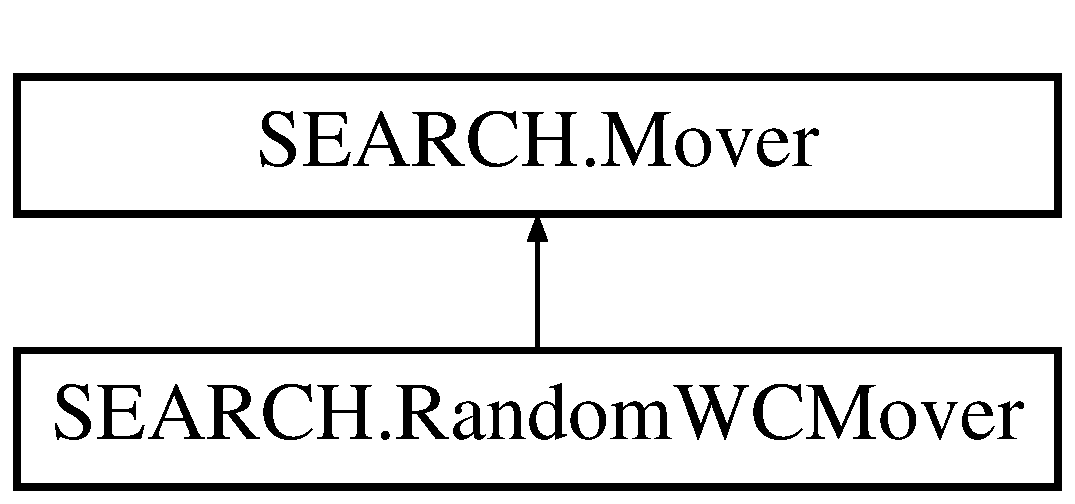
\includegraphics[height=2.000000cm]{class_s_e_a_r_c_h_1_1_random_w_c_mover}
\end{center}
\end{figure}
\subsection*{Public Member Functions}
\begin{DoxyCompactItemize}
\item 
override double \hyperlink{class_s_e_a_r_c_h_1_1_random_w_c_mover_a50f9ef5586b7740beeeb197b7334a560}{get\-Step\-Length} ()
\item 
override double \hyperlink{class_s_e_a_r_c_h_1_1_random_w_c_mover_af859a09b56a19e9e8a772bebbf802142}{get\-Turn\-Angle} (double rho)
\end{DoxyCompactItemize}
\subsection*{Static Public Member Functions}
\begin{DoxyCompactItemize}
\item 
static \hyperlink{class_s_e_a_r_c_h_1_1_random_w_c_mover}{Random\-W\-C\-Mover} \hyperlink{class_s_e_a_r_c_h_1_1_random_w_c_mover_a532c1ff7efb948e0e6e5eeec18263d87}{get\-Random\-W\-C\-Mover} ()
\end{DoxyCompactItemize}
\subsection*{Additional Inherited Members}


\subsection{Detailed Description}
Summary description for \hyperlink{class_s_e_a_r_c_h_1_1_random_w_c_mover}{Random\-W\-C\-Mover}. 



\subsection{Member Function Documentation}
\hypertarget{class_s_e_a_r_c_h_1_1_random_w_c_mover_a532c1ff7efb948e0e6e5eeec18263d87}{\index{S\-E\-A\-R\-C\-H\-::\-Random\-W\-C\-Mover@{S\-E\-A\-R\-C\-H\-::\-Random\-W\-C\-Mover}!get\-Random\-W\-C\-Mover@{get\-Random\-W\-C\-Mover}}
\index{get\-Random\-W\-C\-Mover@{get\-Random\-W\-C\-Mover}!SEARCH::RandomWCMover@{S\-E\-A\-R\-C\-H\-::\-Random\-W\-C\-Mover}}
\subsubsection[{get\-Random\-W\-C\-Mover}]{\setlength{\rightskip}{0pt plus 5cm}static {\bf Random\-W\-C\-Mover} S\-E\-A\-R\-C\-H.\-Random\-W\-C\-Mover.\-get\-Random\-W\-C\-Mover (
\begin{DoxyParamCaption}
{}
\end{DoxyParamCaption}
)\hspace{0.3cm}{\ttfamily [static]}}}\label{class_s_e_a_r_c_h_1_1_random_w_c_mover_a532c1ff7efb948e0e6e5eeec18263d87}
\hypertarget{class_s_e_a_r_c_h_1_1_random_w_c_mover_a50f9ef5586b7740beeeb197b7334a560}{\index{S\-E\-A\-R\-C\-H\-::\-Random\-W\-C\-Mover@{S\-E\-A\-R\-C\-H\-::\-Random\-W\-C\-Mover}!get\-Step\-Length@{get\-Step\-Length}}
\index{get\-Step\-Length@{get\-Step\-Length}!SEARCH::RandomWCMover@{S\-E\-A\-R\-C\-H\-::\-Random\-W\-C\-Mover}}
\subsubsection[{get\-Step\-Length}]{\setlength{\rightskip}{0pt plus 5cm}override double S\-E\-A\-R\-C\-H.\-Random\-W\-C\-Mover.\-get\-Step\-Length (
\begin{DoxyParamCaption}
{}
\end{DoxyParamCaption}
)\hspace{0.3cm}{\ttfamily [virtual]}}}\label{class_s_e_a_r_c_h_1_1_random_w_c_mover_a50f9ef5586b7740beeeb197b7334a560}


Implements \hyperlink{class_s_e_a_r_c_h_1_1_mover_a3e547800bbc34492f4251adee70dbf02}{S\-E\-A\-R\-C\-H.\-Mover}.

\hypertarget{class_s_e_a_r_c_h_1_1_random_w_c_mover_af859a09b56a19e9e8a772bebbf802142}{\index{S\-E\-A\-R\-C\-H\-::\-Random\-W\-C\-Mover@{S\-E\-A\-R\-C\-H\-::\-Random\-W\-C\-Mover}!get\-Turn\-Angle@{get\-Turn\-Angle}}
\index{get\-Turn\-Angle@{get\-Turn\-Angle}!SEARCH::RandomWCMover@{S\-E\-A\-R\-C\-H\-::\-Random\-W\-C\-Mover}}
\subsubsection[{get\-Turn\-Angle}]{\setlength{\rightskip}{0pt plus 5cm}override double S\-E\-A\-R\-C\-H.\-Random\-W\-C\-Mover.\-get\-Turn\-Angle (
\begin{DoxyParamCaption}
\item[{double}]{rho}
\end{DoxyParamCaption}
)\hspace{0.3cm}{\ttfamily [virtual]}}}\label{class_s_e_a_r_c_h_1_1_random_w_c_mover_af859a09b56a19e9e8a772bebbf802142}


Implements \hyperlink{class_s_e_a_r_c_h_1_1_mover_a879a44d5a0c57434375a69c8d8d00e35}{S\-E\-A\-R\-C\-H.\-Mover}.



The documentation for this class was generated from the following file\-:\begin{DoxyCompactItemize}
\item 
Desktop/vlog4net\-A\-R\-C10\-\_\-64\-\_\-newhoming/\-Data\-Centric/\hyperlink{_random_w_c_mover_8cs}{Random\-W\-C\-Mover.\-cs}\end{DoxyCompactItemize}

\hypertarget{class_s_e_a_r_c_h_1_1_resident}{\section{S\-E\-A\-R\-C\-H.\-Resident Class Reference}
\label{class_s_e_a_r_c_h_1_1_resident}\index{S\-E\-A\-R\-C\-H.\-Resident@{S\-E\-A\-R\-C\-H.\-Resident}}
}


Summary description for \hyperlink{class_s_e_a_r_c_h_1_1_resident}{Resident}.  


Inheritance diagram for S\-E\-A\-R\-C\-H.\-Resident\-:\begin{figure}[H]
\begin{center}
\leavevmode
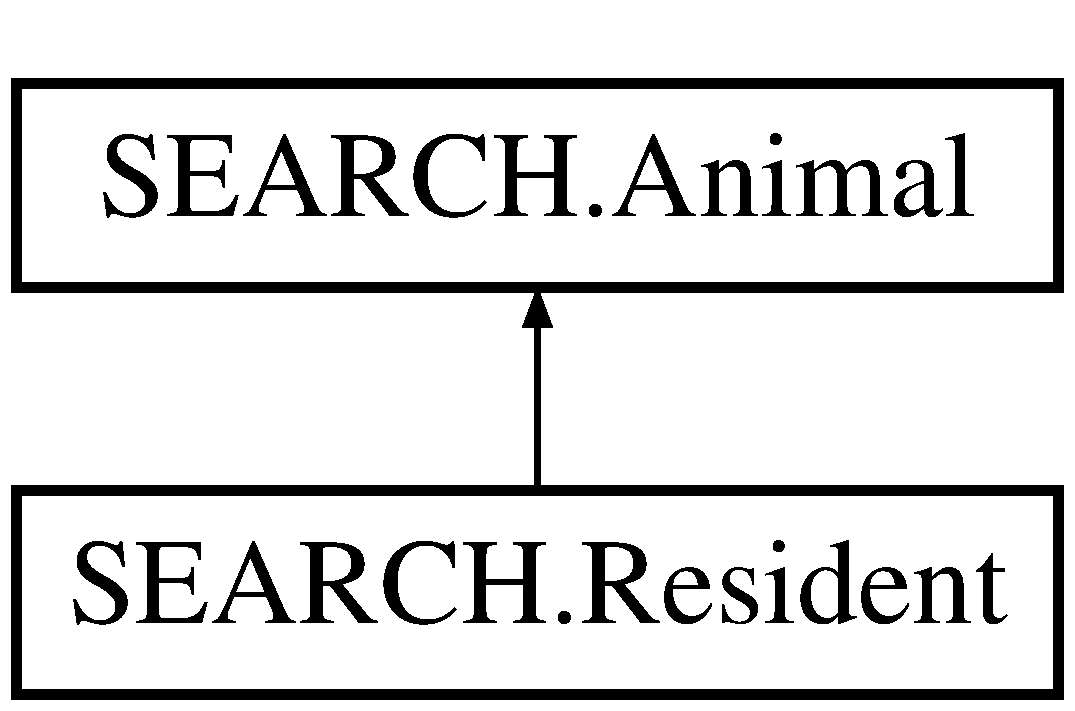
\includegraphics[height=2.000000cm]{class_s_e_a_r_c_h_1_1_resident}
\end{center}
\end{figure}
\subsection*{Public Member Functions}
\begin{DoxyCompactItemize}
\item 
\hyperlink{class_s_e_a_r_c_h_1_1_resident_aece0ff20621058287c6f00696cf13bc6}{Resident} ()
\item 
void \hyperlink{class_s_e_a_r_c_h_1_1_resident_a98f6c7c23ba0c488c86b29552821f804}{breed} (out int num\-Males, out int num\-Females)
\item 
override void \hyperlink{class_s_e_a_r_c_h_1_1_resident_a8b8b9bf2d89bf08618b7649247c98da2}{do\-Time\-Step} (\hyperlink{class_s_e_a_r_c_h_1_1_hourly_modifier}{Hourly\-Modifier} in\-H\-M, \hyperlink{class_s_e_a_r_c_h_1_1_daily_modifier}{Daily\-Modifier} in\-D\-M, Date\-Time curr\-Time, bool do\-Text\-Output, ref string status)
\item 
void \hyperlink{class_s_e_a_r_c_h_1_1_resident_a0130bd18fc8cc7b8e857365a5f1a2f08}{winter\-Kill} (int current\-Time)
\end{DoxyCompactItemize}
\subsection*{Properties}
\begin{DoxyCompactItemize}
\item 
\hyperlink{class_s_e_a_r_c_h_1_1_resident_attributes}{Resident\-Attributes} \hyperlink{class_s_e_a_r_c_h_1_1_resident_a9637f80aa1c0183823803a65d597d485}{My\-Attributes}\hspace{0.3cm}{\ttfamily  \mbox{[}get, set\mbox{]}}
\end{DoxyCompactItemize}
\subsection*{Additional Inherited Members}


\subsection{Detailed Description}
Summary description for \hyperlink{class_s_e_a_r_c_h_1_1_resident}{Resident}. 



\subsection{Constructor \& Destructor Documentation}
\hypertarget{class_s_e_a_r_c_h_1_1_resident_aece0ff20621058287c6f00696cf13bc6}{\index{S\-E\-A\-R\-C\-H\-::\-Resident@{S\-E\-A\-R\-C\-H\-::\-Resident}!Resident@{Resident}}
\index{Resident@{Resident}!SEARCH::Resident@{S\-E\-A\-R\-C\-H\-::\-Resident}}
\subsubsection[{Resident}]{\setlength{\rightskip}{0pt plus 5cm}S\-E\-A\-R\-C\-H.\-Resident.\-Resident (
\begin{DoxyParamCaption}
{}
\end{DoxyParamCaption}
)}}\label{class_s_e_a_r_c_h_1_1_resident_aece0ff20621058287c6f00696cf13bc6}


\subsection{Member Function Documentation}
\hypertarget{class_s_e_a_r_c_h_1_1_resident_a98f6c7c23ba0c488c86b29552821f804}{\index{S\-E\-A\-R\-C\-H\-::\-Resident@{S\-E\-A\-R\-C\-H\-::\-Resident}!breed@{breed}}
\index{breed@{breed}!SEARCH::Resident@{S\-E\-A\-R\-C\-H\-::\-Resident}}
\subsubsection[{breed}]{\setlength{\rightskip}{0pt plus 5cm}void S\-E\-A\-R\-C\-H.\-Resident.\-breed (
\begin{DoxyParamCaption}
\item[{out int}]{num\-Males, }
\item[{out int}]{num\-Females}
\end{DoxyParamCaption}
)}}\label{class_s_e_a_r_c_h_1_1_resident_a98f6c7c23ba0c488c86b29552821f804}
\hypertarget{class_s_e_a_r_c_h_1_1_resident_a8b8b9bf2d89bf08618b7649247c98da2}{\index{S\-E\-A\-R\-C\-H\-::\-Resident@{S\-E\-A\-R\-C\-H\-::\-Resident}!do\-Time\-Step@{do\-Time\-Step}}
\index{do\-Time\-Step@{do\-Time\-Step}!SEARCH::Resident@{S\-E\-A\-R\-C\-H\-::\-Resident}}
\subsubsection[{do\-Time\-Step}]{\setlength{\rightskip}{0pt plus 5cm}override void S\-E\-A\-R\-C\-H.\-Resident.\-do\-Time\-Step (
\begin{DoxyParamCaption}
\item[{{\bf Hourly\-Modifier}}]{in\-H\-M, }
\item[{{\bf Daily\-Modifier}}]{in\-D\-M, }
\item[{Date\-Time}]{curr\-Time, }
\item[{bool}]{do\-Text\-Output, }
\item[{ref string}]{status}
\end{DoxyParamCaption}
)\hspace{0.3cm}{\ttfamily [virtual]}}}\label{class_s_e_a_r_c_h_1_1_resident_a8b8b9bf2d89bf08618b7649247c98da2}


Reimplemented from \hyperlink{class_s_e_a_r_c_h_1_1_animal_ad805d6441c4c873121136b641c404f3a}{S\-E\-A\-R\-C\-H.\-Animal}.

\hypertarget{class_s_e_a_r_c_h_1_1_resident_a0130bd18fc8cc7b8e857365a5f1a2f08}{\index{S\-E\-A\-R\-C\-H\-::\-Resident@{S\-E\-A\-R\-C\-H\-::\-Resident}!winter\-Kill@{winter\-Kill}}
\index{winter\-Kill@{winter\-Kill}!SEARCH::Resident@{S\-E\-A\-R\-C\-H\-::\-Resident}}
\subsubsection[{winter\-Kill}]{\setlength{\rightskip}{0pt plus 5cm}void S\-E\-A\-R\-C\-H.\-Resident.\-winter\-Kill (
\begin{DoxyParamCaption}
\item[{int}]{current\-Time}
\end{DoxyParamCaption}
)}}\label{class_s_e_a_r_c_h_1_1_resident_a0130bd18fc8cc7b8e857365a5f1a2f08}


\subsection{Property Documentation}
\hypertarget{class_s_e_a_r_c_h_1_1_resident_a9637f80aa1c0183823803a65d597d485}{\index{S\-E\-A\-R\-C\-H\-::\-Resident@{S\-E\-A\-R\-C\-H\-::\-Resident}!My\-Attributes@{My\-Attributes}}
\index{My\-Attributes@{My\-Attributes}!SEARCH::Resident@{S\-E\-A\-R\-C\-H\-::\-Resident}}
\subsubsection[{My\-Attributes}]{\setlength{\rightskip}{0pt plus 5cm}{\bf Resident\-Attributes} S\-E\-A\-R\-C\-H.\-Resident.\-My\-Attributes\hspace{0.3cm}{\ttfamily [get]}, {\ttfamily [set]}}}\label{class_s_e_a_r_c_h_1_1_resident_a9637f80aa1c0183823803a65d597d485}


The documentation for this class was generated from the following file\-:\begin{DoxyCompactItemize}
\item 
Desktop/vlog4net\-A\-R\-C10\-\_\-64\-\_\-newhoming/\-Data\-Centric/\hyperlink{_resident_8cs}{Resident.\-cs}\end{DoxyCompactItemize}

\hypertarget{class_s_e_a_r_c_h_1_1_resident_attributes}{\section{S\-E\-A\-R\-C\-H.\-Resident\-Attributes Class Reference}
\label{class_s_e_a_r_c_h_1_1_resident_attributes}\index{S\-E\-A\-R\-C\-H.\-Resident\-Attributes@{S\-E\-A\-R\-C\-H.\-Resident\-Attributes}}
}


Summary description for \hyperlink{class_s_e_a_r_c_h_1_1_resident_attributes}{Resident\-Attributes}.  


\subsection*{Public Member Functions}
\begin{DoxyCompactItemize}
\item 
\hyperlink{class_s_e_a_r_c_h_1_1_resident_attributes_a1c3407543698d67a7a73dec25525447d}{Resident\-Attributes} (double in\-Time\-Risk, double in\-Year\-Risk, double in\-Percent\-Breed, double in\-Percent\-Female, double in\-Mean\-Litter\-Size, double in\-S\-D\-Litter\-Size)
\item 
\hyperlink{class_s_e_a_r_c_h_1_1_resident_attributes_a93eadf31677dde80b5d244f7697c40a3}{Resident\-Attributes} ()
\end{DoxyCompactItemize}
\subsection*{Properties}
\begin{DoxyCompactItemize}
\item 
string \hyperlink{class_s_e_a_r_c_h_1_1_resident_attributes_a0171054fecfa864caac09af157358e9e}{Original\-I\-D}\hspace{0.3cm}{\ttfamily  \mbox{[}get, set\mbox{]}}
\item 
double \hyperlink{class_s_e_a_r_c_h_1_1_resident_attributes_a66a73e69674dea49472e9e58ecba2487}{Percent\-Breed}\hspace{0.3cm}{\ttfamily  \mbox{[}get, set\mbox{]}}
\item 
double \hyperlink{class_s_e_a_r_c_h_1_1_resident_attributes_aba4a0c468662e0a988e4da1f2334ca99}{Percent\-Female}\hspace{0.3cm}{\ttfamily  \mbox{[}get, set\mbox{]}}
\item 
double \hyperlink{class_s_e_a_r_c_h_1_1_resident_attributes_ac8c8ece96750b7903a78b0494b0e76a4}{Num\-Childern\-Mean}\hspace{0.3cm}{\ttfamily  \mbox{[}get, set\mbox{]}}
\item 
double \hyperlink{class_s_e_a_r_c_h_1_1_resident_attributes_afd7000bf05088eb51b9af0a4058c91b3}{Num\-Childern\-S\-D}\hspace{0.3cm}{\ttfamily  \mbox{[}get, set\mbox{]}}
\item 
double \hyperlink{class_s_e_a_r_c_h_1_1_resident_attributes_a235dd77c6271919b4c70387d341ff34d}{Resident\-Time\-Step\-Risk}\hspace{0.3cm}{\ttfamily  \mbox{[}get, set\mbox{]}}
\item 
double \hyperlink{class_s_e_a_r_c_h_1_1_resident_attributes_a4b69906dab69ecf93b1098c65f88cbf3}{Resident\-Yearly\-Risk}\hspace{0.3cm}{\ttfamily  \mbox{[}get, set\mbox{]}}
\end{DoxyCompactItemize}


\subsection{Detailed Description}
Summary description for \hyperlink{class_s_e_a_r_c_h_1_1_resident_attributes}{Resident\-Attributes}. 



\subsection{Constructor \& Destructor Documentation}
\hypertarget{class_s_e_a_r_c_h_1_1_resident_attributes_a1c3407543698d67a7a73dec25525447d}{\index{S\-E\-A\-R\-C\-H\-::\-Resident\-Attributes@{S\-E\-A\-R\-C\-H\-::\-Resident\-Attributes}!Resident\-Attributes@{Resident\-Attributes}}
\index{Resident\-Attributes@{Resident\-Attributes}!SEARCH::ResidentAttributes@{S\-E\-A\-R\-C\-H\-::\-Resident\-Attributes}}
\subsubsection[{Resident\-Attributes}]{\setlength{\rightskip}{0pt plus 5cm}S\-E\-A\-R\-C\-H.\-Resident\-Attributes.\-Resident\-Attributes (
\begin{DoxyParamCaption}
\item[{double}]{in\-Time\-Risk, }
\item[{double}]{in\-Year\-Risk, }
\item[{double}]{in\-Percent\-Breed, }
\item[{double}]{in\-Percent\-Female, }
\item[{double}]{in\-Mean\-Litter\-Size, }
\item[{double}]{in\-S\-D\-Litter\-Size}
\end{DoxyParamCaption}
)}}\label{class_s_e_a_r_c_h_1_1_resident_attributes_a1c3407543698d67a7a73dec25525447d}
\hypertarget{class_s_e_a_r_c_h_1_1_resident_attributes_a93eadf31677dde80b5d244f7697c40a3}{\index{S\-E\-A\-R\-C\-H\-::\-Resident\-Attributes@{S\-E\-A\-R\-C\-H\-::\-Resident\-Attributes}!Resident\-Attributes@{Resident\-Attributes}}
\index{Resident\-Attributes@{Resident\-Attributes}!SEARCH::ResidentAttributes@{S\-E\-A\-R\-C\-H\-::\-Resident\-Attributes}}
\subsubsection[{Resident\-Attributes}]{\setlength{\rightskip}{0pt plus 5cm}S\-E\-A\-R\-C\-H.\-Resident\-Attributes.\-Resident\-Attributes (
\begin{DoxyParamCaption}
{}
\end{DoxyParamCaption}
)}}\label{class_s_e_a_r_c_h_1_1_resident_attributes_a93eadf31677dde80b5d244f7697c40a3}


\subsection{Property Documentation}
\hypertarget{class_s_e_a_r_c_h_1_1_resident_attributes_ac8c8ece96750b7903a78b0494b0e76a4}{\index{S\-E\-A\-R\-C\-H\-::\-Resident\-Attributes@{S\-E\-A\-R\-C\-H\-::\-Resident\-Attributes}!Num\-Childern\-Mean@{Num\-Childern\-Mean}}
\index{Num\-Childern\-Mean@{Num\-Childern\-Mean}!SEARCH::ResidentAttributes@{S\-E\-A\-R\-C\-H\-::\-Resident\-Attributes}}
\subsubsection[{Num\-Childern\-Mean}]{\setlength{\rightskip}{0pt plus 5cm}double S\-E\-A\-R\-C\-H.\-Resident\-Attributes.\-Num\-Childern\-Mean\hspace{0.3cm}{\ttfamily [get]}, {\ttfamily [set]}}}\label{class_s_e_a_r_c_h_1_1_resident_attributes_ac8c8ece96750b7903a78b0494b0e76a4}
\hypertarget{class_s_e_a_r_c_h_1_1_resident_attributes_afd7000bf05088eb51b9af0a4058c91b3}{\index{S\-E\-A\-R\-C\-H\-::\-Resident\-Attributes@{S\-E\-A\-R\-C\-H\-::\-Resident\-Attributes}!Num\-Childern\-S\-D@{Num\-Childern\-S\-D}}
\index{Num\-Childern\-S\-D@{Num\-Childern\-S\-D}!SEARCH::ResidentAttributes@{S\-E\-A\-R\-C\-H\-::\-Resident\-Attributes}}
\subsubsection[{Num\-Childern\-S\-D}]{\setlength{\rightskip}{0pt plus 5cm}double S\-E\-A\-R\-C\-H.\-Resident\-Attributes.\-Num\-Childern\-S\-D\hspace{0.3cm}{\ttfamily [get]}, {\ttfamily [set]}}}\label{class_s_e_a_r_c_h_1_1_resident_attributes_afd7000bf05088eb51b9af0a4058c91b3}
\hypertarget{class_s_e_a_r_c_h_1_1_resident_attributes_a0171054fecfa864caac09af157358e9e}{\index{S\-E\-A\-R\-C\-H\-::\-Resident\-Attributes@{S\-E\-A\-R\-C\-H\-::\-Resident\-Attributes}!Original\-I\-D@{Original\-I\-D}}
\index{Original\-I\-D@{Original\-I\-D}!SEARCH::ResidentAttributes@{S\-E\-A\-R\-C\-H\-::\-Resident\-Attributes}}
\subsubsection[{Original\-I\-D}]{\setlength{\rightskip}{0pt plus 5cm}string S\-E\-A\-R\-C\-H.\-Resident\-Attributes.\-Original\-I\-D\hspace{0.3cm}{\ttfamily [get]}, {\ttfamily [set]}}}\label{class_s_e_a_r_c_h_1_1_resident_attributes_a0171054fecfa864caac09af157358e9e}
\hypertarget{class_s_e_a_r_c_h_1_1_resident_attributes_a66a73e69674dea49472e9e58ecba2487}{\index{S\-E\-A\-R\-C\-H\-::\-Resident\-Attributes@{S\-E\-A\-R\-C\-H\-::\-Resident\-Attributes}!Percent\-Breed@{Percent\-Breed}}
\index{Percent\-Breed@{Percent\-Breed}!SEARCH::ResidentAttributes@{S\-E\-A\-R\-C\-H\-::\-Resident\-Attributes}}
\subsubsection[{Percent\-Breed}]{\setlength{\rightskip}{0pt plus 5cm}double S\-E\-A\-R\-C\-H.\-Resident\-Attributes.\-Percent\-Breed\hspace{0.3cm}{\ttfamily [get]}, {\ttfamily [set]}}}\label{class_s_e_a_r_c_h_1_1_resident_attributes_a66a73e69674dea49472e9e58ecba2487}
\hypertarget{class_s_e_a_r_c_h_1_1_resident_attributes_aba4a0c468662e0a988e4da1f2334ca99}{\index{S\-E\-A\-R\-C\-H\-::\-Resident\-Attributes@{S\-E\-A\-R\-C\-H\-::\-Resident\-Attributes}!Percent\-Female@{Percent\-Female}}
\index{Percent\-Female@{Percent\-Female}!SEARCH::ResidentAttributes@{S\-E\-A\-R\-C\-H\-::\-Resident\-Attributes}}
\subsubsection[{Percent\-Female}]{\setlength{\rightskip}{0pt plus 5cm}double S\-E\-A\-R\-C\-H.\-Resident\-Attributes.\-Percent\-Female\hspace{0.3cm}{\ttfamily [get]}, {\ttfamily [set]}}}\label{class_s_e_a_r_c_h_1_1_resident_attributes_aba4a0c468662e0a988e4da1f2334ca99}
\hypertarget{class_s_e_a_r_c_h_1_1_resident_attributes_a235dd77c6271919b4c70387d341ff34d}{\index{S\-E\-A\-R\-C\-H\-::\-Resident\-Attributes@{S\-E\-A\-R\-C\-H\-::\-Resident\-Attributes}!Resident\-Time\-Step\-Risk@{Resident\-Time\-Step\-Risk}}
\index{Resident\-Time\-Step\-Risk@{Resident\-Time\-Step\-Risk}!SEARCH::ResidentAttributes@{S\-E\-A\-R\-C\-H\-::\-Resident\-Attributes}}
\subsubsection[{Resident\-Time\-Step\-Risk}]{\setlength{\rightskip}{0pt plus 5cm}double S\-E\-A\-R\-C\-H.\-Resident\-Attributes.\-Resident\-Time\-Step\-Risk\hspace{0.3cm}{\ttfamily [get]}, {\ttfamily [set]}}}\label{class_s_e_a_r_c_h_1_1_resident_attributes_a235dd77c6271919b4c70387d341ff34d}
\hypertarget{class_s_e_a_r_c_h_1_1_resident_attributes_a4b69906dab69ecf93b1098c65f88cbf3}{\index{S\-E\-A\-R\-C\-H\-::\-Resident\-Attributes@{S\-E\-A\-R\-C\-H\-::\-Resident\-Attributes}!Resident\-Yearly\-Risk@{Resident\-Yearly\-Risk}}
\index{Resident\-Yearly\-Risk@{Resident\-Yearly\-Risk}!SEARCH::ResidentAttributes@{S\-E\-A\-R\-C\-H\-::\-Resident\-Attributes}}
\subsubsection[{Resident\-Yearly\-Risk}]{\setlength{\rightskip}{0pt plus 5cm}double S\-E\-A\-R\-C\-H.\-Resident\-Attributes.\-Resident\-Yearly\-Risk\hspace{0.3cm}{\ttfamily [get]}, {\ttfamily [set]}}}\label{class_s_e_a_r_c_h_1_1_resident_attributes_a4b69906dab69ecf93b1098c65f88cbf3}


The documentation for this class was generated from the following file\-:\begin{DoxyCompactItemize}
\item 
Desktop/vlog4net\-A\-R\-C10\-\_\-64\-\_\-newhoming/\-Data\-Centric/\hyperlink{_resident_attributes_8cs}{Resident\-Attributes.\-cs}\end{DoxyCompactItemize}

\hypertarget{class_s_e_a_r_c_h_1_1_resting}{\section{S\-E\-A\-R\-C\-H.\-Resting Class Reference}
\label{class_s_e_a_r_c_h_1_1_resting}\index{S\-E\-A\-R\-C\-H.\-Resting@{S\-E\-A\-R\-C\-H.\-Resting}}
}
Inheritance diagram for S\-E\-A\-R\-C\-H.\-Resting\-:\begin{figure}[H]
\begin{center}
\leavevmode
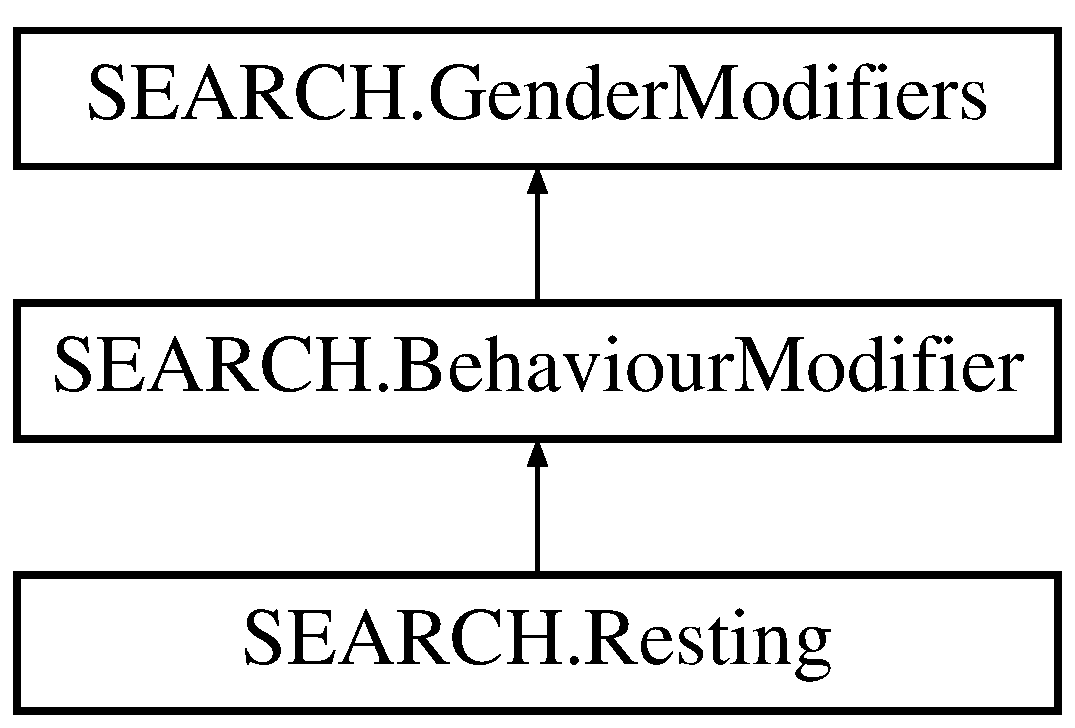
\includegraphics[height=3.000000cm]{class_s_e_a_r_c_h_1_1_resting}
\end{center}
\end{figure}
\subsection*{Additional Inherited Members}


The documentation for this class was generated from the following file\-:\begin{DoxyCompactItemize}
\item 
Desktop/vlog4net\-A\-R\-C10\-\_\-64\-\_\-newhoming/\-Data\-Centric/\hyperlink{_resting_8cs}{Resting.\-cs}\end{DoxyCompactItemize}

\hypertarget{class_s_e_a_r_c_h_1_1_risky_forage_modifier}{\section{S\-E\-A\-R\-C\-H.\-Risky\-Forage\-Modifier Class Reference}
\label{class_s_e_a_r_c_h_1_1_risky_forage_modifier}\index{S\-E\-A\-R\-C\-H.\-Risky\-Forage\-Modifier@{S\-E\-A\-R\-C\-H.\-Risky\-Forage\-Modifier}}
}
Inheritance diagram for S\-E\-A\-R\-C\-H.\-Risky\-Forage\-Modifier\-:\begin{figure}[H]
\begin{center}
\leavevmode
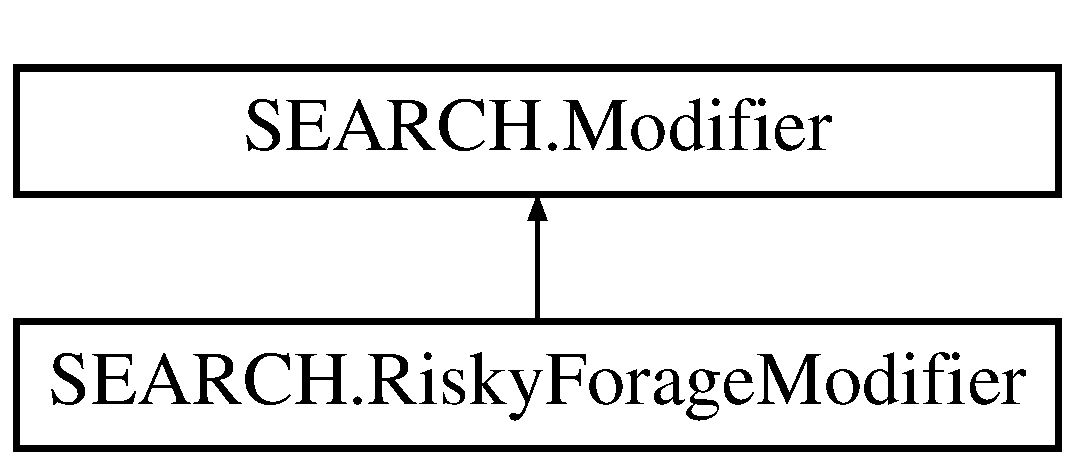
\includegraphics[height=2.000000cm]{class_s_e_a_r_c_h_1_1_risky_forage_modifier}
\end{center}
\end{figure}
\subsection*{Public Member Functions}
\begin{DoxyCompactItemize}
\item 
\hyperlink{class_s_e_a_r_c_h_1_1_risky_forage_modifier_a6c52aef9da5d17bfbe6f68ea204c6280}{Risky\-Forage\-Modifier} ()
\end{DoxyCompactItemize}
\subsection*{Additional Inherited Members}


\subsection{Constructor \& Destructor Documentation}
\hypertarget{class_s_e_a_r_c_h_1_1_risky_forage_modifier_a6c52aef9da5d17bfbe6f68ea204c6280}{\index{S\-E\-A\-R\-C\-H\-::\-Risky\-Forage\-Modifier@{S\-E\-A\-R\-C\-H\-::\-Risky\-Forage\-Modifier}!Risky\-Forage\-Modifier@{Risky\-Forage\-Modifier}}
\index{Risky\-Forage\-Modifier@{Risky\-Forage\-Modifier}!SEARCH::RiskyForageModifier@{S\-E\-A\-R\-C\-H\-::\-Risky\-Forage\-Modifier}}
\subsubsection[{Risky\-Forage\-Modifier}]{\setlength{\rightskip}{0pt plus 5cm}S\-E\-A\-R\-C\-H.\-Risky\-Forage\-Modifier.\-Risky\-Forage\-Modifier (
\begin{DoxyParamCaption}
{}
\end{DoxyParamCaption}
)}}\label{class_s_e_a_r_c_h_1_1_risky_forage_modifier_a6c52aef9da5d17bfbe6f68ea204c6280}


The documentation for this class was generated from the following file\-:\begin{DoxyCompactItemize}
\item 
Desktop/vlog4net\-A\-R\-C10\-\_\-64\-\_\-newhoming/\-Data\-Centric/\hyperlink{_risky_forage_8cs}{Risky\-Forage.\-cs}\end{DoxyCompactItemize}

\hypertarget{class_s_e_a_r_c_h_1_1_risky_search_modifier}{\section{S\-E\-A\-R\-C\-H.\-Risky\-Search\-Modifier Class Reference}
\label{class_s_e_a_r_c_h_1_1_risky_search_modifier}\index{S\-E\-A\-R\-C\-H.\-Risky\-Search\-Modifier@{S\-E\-A\-R\-C\-H.\-Risky\-Search\-Modifier}}
}
Inheritance diagram for S\-E\-A\-R\-C\-H.\-Risky\-Search\-Modifier\-:\begin{figure}[H]
\begin{center}
\leavevmode
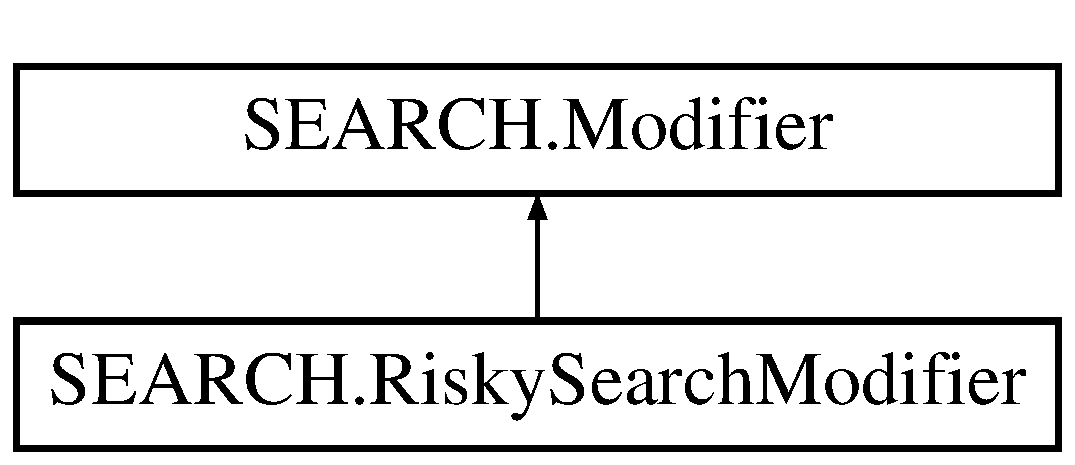
\includegraphics[height=2.000000cm]{class_s_e_a_r_c_h_1_1_risky_search_modifier}
\end{center}
\end{figure}
\subsection*{Public Member Functions}
\begin{DoxyCompactItemize}
\item 
\hyperlink{class_s_e_a_r_c_h_1_1_risky_search_modifier_ab4ac6c006d31baec11c3968475031928}{Risky\-Search\-Modifier} ()
\end{DoxyCompactItemize}
\subsection*{Additional Inherited Members}


\subsection{Constructor \& Destructor Documentation}
\hypertarget{class_s_e_a_r_c_h_1_1_risky_search_modifier_ab4ac6c006d31baec11c3968475031928}{\index{S\-E\-A\-R\-C\-H\-::\-Risky\-Search\-Modifier@{S\-E\-A\-R\-C\-H\-::\-Risky\-Search\-Modifier}!Risky\-Search\-Modifier@{Risky\-Search\-Modifier}}
\index{Risky\-Search\-Modifier@{Risky\-Search\-Modifier}!SEARCH::RiskySearchModifier@{S\-E\-A\-R\-C\-H\-::\-Risky\-Search\-Modifier}}
\subsubsection[{Risky\-Search\-Modifier}]{\setlength{\rightskip}{0pt plus 5cm}S\-E\-A\-R\-C\-H.\-Risky\-Search\-Modifier.\-Risky\-Search\-Modifier (
\begin{DoxyParamCaption}
{}
\end{DoxyParamCaption}
)}}\label{class_s_e_a_r_c_h_1_1_risky_search_modifier_ab4ac6c006d31baec11c3968475031928}


The documentation for this class was generated from the following file\-:\begin{DoxyCompactItemize}
\item 
Desktop/vlog4net\-A\-R\-C10\-\_\-64\-\_\-newhoming/\-Data\-Centric/\hyperlink{_risky_search_8cs}{Risky\-Search.\-cs}\end{DoxyCompactItemize}

\hypertarget{class_s_e_a_r_c_h_1_1_safe_forage_modifier}{\section{S\-E\-A\-R\-C\-H.\-Safe\-Forage\-Modifier Class Reference}
\label{class_s_e_a_r_c_h_1_1_safe_forage_modifier}\index{S\-E\-A\-R\-C\-H.\-Safe\-Forage\-Modifier@{S\-E\-A\-R\-C\-H.\-Safe\-Forage\-Modifier}}
}
Inheritance diagram for S\-E\-A\-R\-C\-H.\-Safe\-Forage\-Modifier\-:\begin{figure}[H]
\begin{center}
\leavevmode
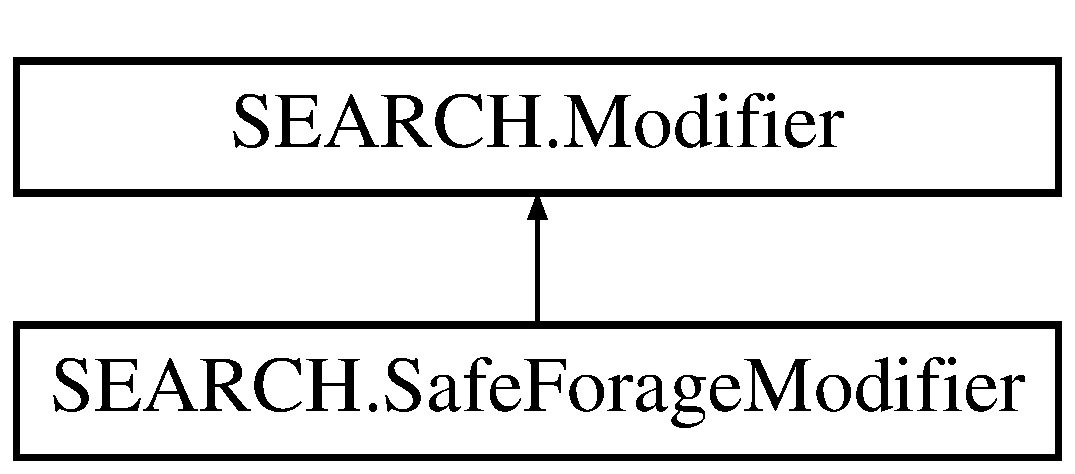
\includegraphics[height=2.000000cm]{class_s_e_a_r_c_h_1_1_safe_forage_modifier}
\end{center}
\end{figure}
\subsection*{Public Member Functions}
\begin{DoxyCompactItemize}
\item 
\hyperlink{class_s_e_a_r_c_h_1_1_safe_forage_modifier_a26c44066ae7ad43067377a51b94b1eb2}{Safe\-Forage\-Modifier} ()
\end{DoxyCompactItemize}
\subsection*{Additional Inherited Members}


\subsection{Constructor \& Destructor Documentation}
\hypertarget{class_s_e_a_r_c_h_1_1_safe_forage_modifier_a26c44066ae7ad43067377a51b94b1eb2}{\index{S\-E\-A\-R\-C\-H\-::\-Safe\-Forage\-Modifier@{S\-E\-A\-R\-C\-H\-::\-Safe\-Forage\-Modifier}!Safe\-Forage\-Modifier@{Safe\-Forage\-Modifier}}
\index{Safe\-Forage\-Modifier@{Safe\-Forage\-Modifier}!SEARCH::SafeForageModifier@{S\-E\-A\-R\-C\-H\-::\-Safe\-Forage\-Modifier}}
\subsubsection[{Safe\-Forage\-Modifier}]{\setlength{\rightskip}{0pt plus 5cm}S\-E\-A\-R\-C\-H.\-Safe\-Forage\-Modifier.\-Safe\-Forage\-Modifier (
\begin{DoxyParamCaption}
{}
\end{DoxyParamCaption}
)}}\label{class_s_e_a_r_c_h_1_1_safe_forage_modifier_a26c44066ae7ad43067377a51b94b1eb2}


The documentation for this class was generated from the following file\-:\begin{DoxyCompactItemize}
\item 
Desktop/vlog4net\-A\-R\-C10\-\_\-64\-\_\-newhoming/\-Data\-Centric/\hyperlink{_safe_forage_8cs}{Safe\-Forage.\-cs}\end{DoxyCompactItemize}

\hypertarget{class_s_e_a_r_c_h_1_1_safe_search_modifier}{\section{S\-E\-A\-R\-C\-H.\-Safe\-Search\-Modifier Class Reference}
\label{class_s_e_a_r_c_h_1_1_safe_search_modifier}\index{S\-E\-A\-R\-C\-H.\-Safe\-Search\-Modifier@{S\-E\-A\-R\-C\-H.\-Safe\-Search\-Modifier}}
}
Inheritance diagram for S\-E\-A\-R\-C\-H.\-Safe\-Search\-Modifier\-:\begin{figure}[H]
\begin{center}
\leavevmode
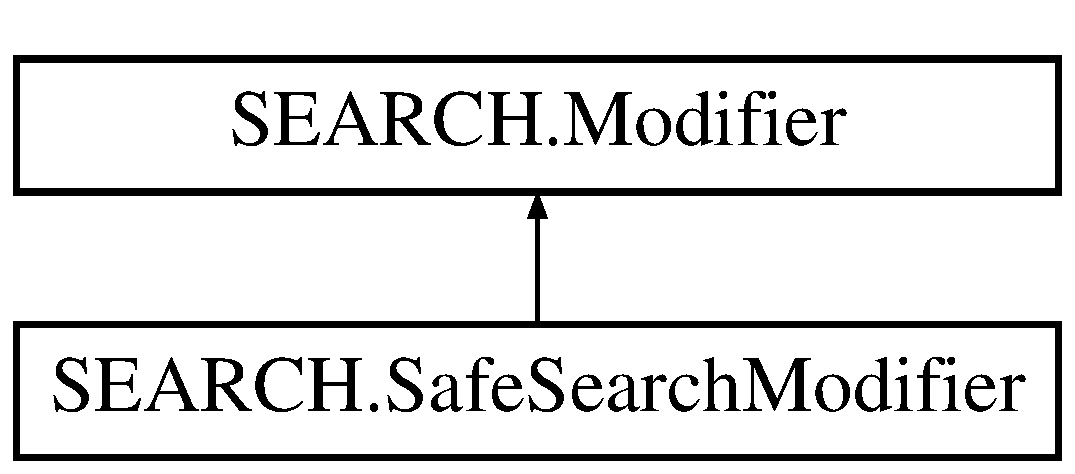
\includegraphics[height=2.000000cm]{class_s_e_a_r_c_h_1_1_safe_search_modifier}
\end{center}
\end{figure}
\subsection*{Public Member Functions}
\begin{DoxyCompactItemize}
\item 
\hyperlink{class_s_e_a_r_c_h_1_1_safe_search_modifier_ab030271cb8d72c9b4e13d5fadc61535c}{Safe\-Search\-Modifier} ()
\end{DoxyCompactItemize}
\subsection*{Additional Inherited Members}


\subsection{Constructor \& Destructor Documentation}
\hypertarget{class_s_e_a_r_c_h_1_1_safe_search_modifier_ab030271cb8d72c9b4e13d5fadc61535c}{\index{S\-E\-A\-R\-C\-H\-::\-Safe\-Search\-Modifier@{S\-E\-A\-R\-C\-H\-::\-Safe\-Search\-Modifier}!Safe\-Search\-Modifier@{Safe\-Search\-Modifier}}
\index{Safe\-Search\-Modifier@{Safe\-Search\-Modifier}!SEARCH::SafeSearchModifier@{S\-E\-A\-R\-C\-H\-::\-Safe\-Search\-Modifier}}
\subsubsection[{Safe\-Search\-Modifier}]{\setlength{\rightskip}{0pt plus 5cm}S\-E\-A\-R\-C\-H.\-Safe\-Search\-Modifier.\-Safe\-Search\-Modifier (
\begin{DoxyParamCaption}
{}
\end{DoxyParamCaption}
)}}\label{class_s_e_a_r_c_h_1_1_safe_search_modifier_ab030271cb8d72c9b4e13d5fadc61535c}


The documentation for this class was generated from the following file\-:\begin{DoxyCompactItemize}
\item 
Desktop/vlog4net\-A\-R\-C10\-\_\-64\-\_\-newhoming/\-Data\-Centric/\hyperlink{_safe_search_8cs}{Safe\-Search.\-cs}\end{DoxyCompactItemize}

\hypertarget{class_s_e_a_r_c_h_1_1_simulaton_manager}{\section{S\-E\-A\-R\-C\-H.\-Simulaton\-Manager Class Reference}
\label{class_s_e_a_r_c_h_1_1_simulaton_manager}\index{S\-E\-A\-R\-C\-H.\-Simulaton\-Manager@{S\-E\-A\-R\-C\-H.\-Simulaton\-Manager}}
}


-\/\-The Client asks the Singleton to get its unique instance . It accesses a Singleton instance solely through Singleton's Instance operation.  


\subsection*{Public Member Functions}
\begin{DoxyCompactItemize}
\item 
\hyperlink{class_s_e_a_r_c_h_1_1_simulaton_manager_a95ad0a5a8dbe4988d71d7a677a70769e}{Simulaton\-Manager} ()
\item 
void \hyperlink{class_s_e_a_r_c_h_1_1_simulaton_manager_a9657bba4a36ac70cecf22c35b8112298}{add\-Daily\-Modifier} (\hyperlink{class_s_e_a_r_c_h_1_1_daily_modifier}{Daily\-Modifier} in\-D\-M)
\item 
void \hyperlink{class_s_e_a_r_c_h_1_1_simulaton_manager_aab0124936a4fe932e3803527f996faca}{add\-Hourly\-Modifier} (\hyperlink{class_s_e_a_r_c_h_1_1_hourly_modifier}{Hourly\-Modifier} in\-Hm)
\item 
bool \hyperlink{class_s_e_a_r_c_h_1_1_simulaton_manager_a6c48b286777a875e82efaf8f9cf4cd72}{build\-Animals} ()
\item 
bool \hyperlink{class_s_e_a_r_c_h_1_1_simulaton_manager_a16ff580d96ea8e1fa4fd3dc08d6a5e61}{build\-Residents} ()
\item 
void \hyperlink{class_s_e_a_r_c_h_1_1_simulaton_manager_ada1ed055be96685ccca12dd6e6d1dc4a}{do\-Simulation} (\hyperlink{class_s_e_a_r_c_h_1_1frm_input}{frm\-Input} in\-Form)
\item 
bool \hyperlink{class_s_e_a_r_c_h_1_1_simulaton_manager_aab843881bab783ac55bcaafd0b4609d1}{make\-Initial\-Animal\-Maps} ()
\item 
bool \hyperlink{class_s_e_a_r_c_h_1_1_simulaton_manager_ab960c75bf04a58e10cbe47b2712cfbcc}{make\-Resident\-Maps} ()
\item 
bool \hyperlink{class_s_e_a_r_c_h_1_1_simulaton_manager_a803d588dfdc97b9d788c08031e170939}{make\-Temp\-Map} (string path)
\item 
void \hyperlink{class_s_e_a_r_c_h_1_1_simulaton_manager_a0ba373c5f331bd9224a0c00bb8e1705c}{set\-Residents\-Text\-Out\-Put} (string path)
\item 
bool \hyperlink{class_s_e_a_r_c_h_1_1_simulaton_manager_ae03bae84f1c0a77c2fdca0107cc20189}{set\-Resident\-Attributes} (double in\-Time\-Step\-Risk, double in\-Yearly\-Risk, double in\-Percent\-Breed, double in\-Percent\-Female, double in\-Mean\-Litter\-Size, double in\-S\-D\-Litter\-Size)
\end{DoxyCompactItemize}
\subsection*{Properties}
\begin{DoxyCompactItemize}
\item 
\hyperlink{class_s_e_a_r_c_h_1_1_animal_manager}{Animal\-Manager} \hyperlink{class_s_e_a_r_c_h_1_1_simulaton_manager_a973ada3841ee555105f7924b2686f1d4}{Animal\-Manager}\hspace{0.3cm}{\ttfamily  \mbox{[}get, set\mbox{]}}
\item 
bool \hyperlink{class_s_e_a_r_c_h_1_1_simulaton_manager_af30500a864ff11f63588abdb37b2e088}{Do\-Text\-Out\-Put}\hspace{0.3cm}{\ttfamily  \mbox{[}get, set\mbox{]}}
\item 
double \hyperlink{class_s_e_a_r_c_h_1_1_simulaton_manager_a4330d8b9acc4030ed87e68946c9c08e7}{Elapsed\-Time\-Between\-Time\-Step}\hspace{0.3cm}{\ttfamily  \mbox{[}get, set\mbox{]}}
\item 
Date\-Time \hyperlink{class_s_e_a_r_c_h_1_1_simulaton_manager_ad2e4b697ea8f94a61ec5a1fc18b5d61e}{End\-Season\-Date}\hspace{0.3cm}{\ttfamily  \mbox{[}get, set\mbox{]}}
\item 
Date\-Time \hyperlink{class_s_e_a_r_c_h_1_1_simulaton_manager_a32cb04f903957d18c0d69463584f5bca}{End\-Simulaton\-Date}\hspace{0.3cm}{\ttfamily  \mbox{[}get, set\mbox{]}}
\item 
string \hyperlink{class_s_e_a_r_c_h_1_1_simulaton_manager_aaadb2a776a0a68224eea1fb757677cd5}{Err\-Message}\hspace{0.3cm}{\ttfamily  \mbox{[}get, set\mbox{]}}
\item 
\hyperlink{class_s_e_a_r_c_h_1_1_map_manager}{Map\-Manager} \hyperlink{class_s_e_a_r_c_h_1_1_simulaton_manager_a74157972d3b6ef60e20edceddec3f1c4}{Map\-Manager}\hspace{0.3cm}{\ttfamily  \mbox{[}get, set\mbox{]}}
\item 
string \hyperlink{class_s_e_a_r_c_h_1_1_simulaton_manager_a7f17624a62673a19589d21ba614e243a}{Map\-Out\-Put\-Path}\hspace{0.3cm}{\ttfamily  \mbox{[}get, set\mbox{]}}
\item 
int \hyperlink{class_s_e_a_r_c_h_1_1_simulaton_manager_ae6d6a9635f0b3866305e128d3e531cb1}{Num\-Days\-Season}\hspace{0.3cm}{\ttfamily  \mbox{[}get, set\mbox{]}}
\item 
int \hyperlink{class_s_e_a_r_c_h_1_1_simulaton_manager_ae0c2642afa2afc728ebd0b6aed63fccd}{Num\-Seasons}\hspace{0.3cm}{\ttfamily  \mbox{[}get, set\mbox{]}}
\item 
Date\-Time \hyperlink{class_s_e_a_r_c_h_1_1_simulaton_manager_a3d2b067d7bcbb09387ce086fff4778a5}{Start\-Season\-Date}\hspace{0.3cm}{\ttfamily  \mbox{[}get, set\mbox{]}}
\item 
Date\-Time \hyperlink{class_s_e_a_r_c_h_1_1_simulaton_manager_a97422d3d9b72cfc76e05f55f903d9833}{Start\-Simulation\-Date}\hspace{0.3cm}{\ttfamily  \mbox{[}get, set\mbox{]}}
\item 
string \hyperlink{class_s_e_a_r_c_h_1_1_simulaton_manager_a98b5aed35f8e2da23b5b099487e0a57c}{Text\-Out\-Put\-File\-Name}\hspace{0.3cm}{\ttfamily  \mbox{[}get, set\mbox{]}}
\end{DoxyCompactItemize}


\subsection{Detailed Description}
-\/\-The Client asks the Singleton to get its unique instance . It accesses a Singleton instance solely through Singleton's Instance operation. 



\subsection{Constructor \& Destructor Documentation}
\hypertarget{class_s_e_a_r_c_h_1_1_simulaton_manager_a95ad0a5a8dbe4988d71d7a677a70769e}{\index{S\-E\-A\-R\-C\-H\-::\-Simulaton\-Manager@{S\-E\-A\-R\-C\-H\-::\-Simulaton\-Manager}!Simulaton\-Manager@{Simulaton\-Manager}}
\index{Simulaton\-Manager@{Simulaton\-Manager}!SEARCH::SimulatonManager@{S\-E\-A\-R\-C\-H\-::\-Simulaton\-Manager}}
\subsubsection[{Simulaton\-Manager}]{\setlength{\rightskip}{0pt plus 5cm}S\-E\-A\-R\-C\-H.\-Simulaton\-Manager.\-Simulaton\-Manager (
\begin{DoxyParamCaption}
{}
\end{DoxyParamCaption}
)}}\label{class_s_e_a_r_c_h_1_1_simulaton_manager_a95ad0a5a8dbe4988d71d7a677a70769e}


\subsection{Member Function Documentation}
\hypertarget{class_s_e_a_r_c_h_1_1_simulaton_manager_a9657bba4a36ac70cecf22c35b8112298}{\index{S\-E\-A\-R\-C\-H\-::\-Simulaton\-Manager@{S\-E\-A\-R\-C\-H\-::\-Simulaton\-Manager}!add\-Daily\-Modifier@{add\-Daily\-Modifier}}
\index{add\-Daily\-Modifier@{add\-Daily\-Modifier}!SEARCH::SimulatonManager@{S\-E\-A\-R\-C\-H\-::\-Simulaton\-Manager}}
\subsubsection[{add\-Daily\-Modifier}]{\setlength{\rightskip}{0pt plus 5cm}void S\-E\-A\-R\-C\-H.\-Simulaton\-Manager.\-add\-Daily\-Modifier (
\begin{DoxyParamCaption}
\item[{{\bf Daily\-Modifier}}]{in\-D\-M}
\end{DoxyParamCaption}
)}}\label{class_s_e_a_r_c_h_1_1_simulaton_manager_a9657bba4a36ac70cecf22c35b8112298}
\hypertarget{class_s_e_a_r_c_h_1_1_simulaton_manager_aab0124936a4fe932e3803527f996faca}{\index{S\-E\-A\-R\-C\-H\-::\-Simulaton\-Manager@{S\-E\-A\-R\-C\-H\-::\-Simulaton\-Manager}!add\-Hourly\-Modifier@{add\-Hourly\-Modifier}}
\index{add\-Hourly\-Modifier@{add\-Hourly\-Modifier}!SEARCH::SimulatonManager@{S\-E\-A\-R\-C\-H\-::\-Simulaton\-Manager}}
\subsubsection[{add\-Hourly\-Modifier}]{\setlength{\rightskip}{0pt plus 5cm}void S\-E\-A\-R\-C\-H.\-Simulaton\-Manager.\-add\-Hourly\-Modifier (
\begin{DoxyParamCaption}
\item[{{\bf Hourly\-Modifier}}]{in\-Hm}
\end{DoxyParamCaption}
)}}\label{class_s_e_a_r_c_h_1_1_simulaton_manager_aab0124936a4fe932e3803527f996faca}
\hypertarget{class_s_e_a_r_c_h_1_1_simulaton_manager_a6c48b286777a875e82efaf8f9cf4cd72}{\index{S\-E\-A\-R\-C\-H\-::\-Simulaton\-Manager@{S\-E\-A\-R\-C\-H\-::\-Simulaton\-Manager}!build\-Animals@{build\-Animals}}
\index{build\-Animals@{build\-Animals}!SEARCH::SimulatonManager@{S\-E\-A\-R\-C\-H\-::\-Simulaton\-Manager}}
\subsubsection[{build\-Animals}]{\setlength{\rightskip}{0pt plus 5cm}bool S\-E\-A\-R\-C\-H.\-Simulaton\-Manager.\-build\-Animals (
\begin{DoxyParamCaption}
{}
\end{DoxyParamCaption}
)}}\label{class_s_e_a_r_c_h_1_1_simulaton_manager_a6c48b286777a875e82efaf8f9cf4cd72}
\hypertarget{class_s_e_a_r_c_h_1_1_simulaton_manager_a16ff580d96ea8e1fa4fd3dc08d6a5e61}{\index{S\-E\-A\-R\-C\-H\-::\-Simulaton\-Manager@{S\-E\-A\-R\-C\-H\-::\-Simulaton\-Manager}!build\-Residents@{build\-Residents}}
\index{build\-Residents@{build\-Residents}!SEARCH::SimulatonManager@{S\-E\-A\-R\-C\-H\-::\-Simulaton\-Manager}}
\subsubsection[{build\-Residents}]{\setlength{\rightskip}{0pt plus 5cm}bool S\-E\-A\-R\-C\-H.\-Simulaton\-Manager.\-build\-Residents (
\begin{DoxyParamCaption}
{}
\end{DoxyParamCaption}
)}}\label{class_s_e_a_r_c_h_1_1_simulaton_manager_a16ff580d96ea8e1fa4fd3dc08d6a5e61}
\hypertarget{class_s_e_a_r_c_h_1_1_simulaton_manager_ada1ed055be96685ccca12dd6e6d1dc4a}{\index{S\-E\-A\-R\-C\-H\-::\-Simulaton\-Manager@{S\-E\-A\-R\-C\-H\-::\-Simulaton\-Manager}!do\-Simulation@{do\-Simulation}}
\index{do\-Simulation@{do\-Simulation}!SEARCH::SimulatonManager@{S\-E\-A\-R\-C\-H\-::\-Simulaton\-Manager}}
\subsubsection[{do\-Simulation}]{\setlength{\rightskip}{0pt plus 5cm}void S\-E\-A\-R\-C\-H.\-Simulaton\-Manager.\-do\-Simulation (
\begin{DoxyParamCaption}
\item[{{\bf frm\-Input}}]{in\-Form}
\end{DoxyParamCaption}
)}}\label{class_s_e_a_r_c_h_1_1_simulaton_manager_ada1ed055be96685ccca12dd6e6d1dc4a}
\hypertarget{class_s_e_a_r_c_h_1_1_simulaton_manager_aab843881bab783ac55bcaafd0b4609d1}{\index{S\-E\-A\-R\-C\-H\-::\-Simulaton\-Manager@{S\-E\-A\-R\-C\-H\-::\-Simulaton\-Manager}!make\-Initial\-Animal\-Maps@{make\-Initial\-Animal\-Maps}}
\index{make\-Initial\-Animal\-Maps@{make\-Initial\-Animal\-Maps}!SEARCH::SimulatonManager@{S\-E\-A\-R\-C\-H\-::\-Simulaton\-Manager}}
\subsubsection[{make\-Initial\-Animal\-Maps}]{\setlength{\rightskip}{0pt plus 5cm}bool S\-E\-A\-R\-C\-H.\-Simulaton\-Manager.\-make\-Initial\-Animal\-Maps (
\begin{DoxyParamCaption}
{}
\end{DoxyParamCaption}
)}}\label{class_s_e_a_r_c_h_1_1_simulaton_manager_aab843881bab783ac55bcaafd0b4609d1}
\hypertarget{class_s_e_a_r_c_h_1_1_simulaton_manager_ab960c75bf04a58e10cbe47b2712cfbcc}{\index{S\-E\-A\-R\-C\-H\-::\-Simulaton\-Manager@{S\-E\-A\-R\-C\-H\-::\-Simulaton\-Manager}!make\-Resident\-Maps@{make\-Resident\-Maps}}
\index{make\-Resident\-Maps@{make\-Resident\-Maps}!SEARCH::SimulatonManager@{S\-E\-A\-R\-C\-H\-::\-Simulaton\-Manager}}
\subsubsection[{make\-Resident\-Maps}]{\setlength{\rightskip}{0pt plus 5cm}bool S\-E\-A\-R\-C\-H.\-Simulaton\-Manager.\-make\-Resident\-Maps (
\begin{DoxyParamCaption}
{}
\end{DoxyParamCaption}
)}}\label{class_s_e_a_r_c_h_1_1_simulaton_manager_ab960c75bf04a58e10cbe47b2712cfbcc}
\hypertarget{class_s_e_a_r_c_h_1_1_simulaton_manager_a803d588dfdc97b9d788c08031e170939}{\index{S\-E\-A\-R\-C\-H\-::\-Simulaton\-Manager@{S\-E\-A\-R\-C\-H\-::\-Simulaton\-Manager}!make\-Temp\-Map@{make\-Temp\-Map}}
\index{make\-Temp\-Map@{make\-Temp\-Map}!SEARCH::SimulatonManager@{S\-E\-A\-R\-C\-H\-::\-Simulaton\-Manager}}
\subsubsection[{make\-Temp\-Map}]{\setlength{\rightskip}{0pt plus 5cm}bool S\-E\-A\-R\-C\-H.\-Simulaton\-Manager.\-make\-Temp\-Map (
\begin{DoxyParamCaption}
\item[{string}]{path}
\end{DoxyParamCaption}
)}}\label{class_s_e_a_r_c_h_1_1_simulaton_manager_a803d588dfdc97b9d788c08031e170939}
\hypertarget{class_s_e_a_r_c_h_1_1_simulaton_manager_ae03bae84f1c0a77c2fdca0107cc20189}{\index{S\-E\-A\-R\-C\-H\-::\-Simulaton\-Manager@{S\-E\-A\-R\-C\-H\-::\-Simulaton\-Manager}!set\-Resident\-Attributes@{set\-Resident\-Attributes}}
\index{set\-Resident\-Attributes@{set\-Resident\-Attributes}!SEARCH::SimulatonManager@{S\-E\-A\-R\-C\-H\-::\-Simulaton\-Manager}}
\subsubsection[{set\-Resident\-Attributes}]{\setlength{\rightskip}{0pt plus 5cm}bool S\-E\-A\-R\-C\-H.\-Simulaton\-Manager.\-set\-Resident\-Attributes (
\begin{DoxyParamCaption}
\item[{double}]{in\-Time\-Step\-Risk, }
\item[{double}]{in\-Yearly\-Risk, }
\item[{double}]{in\-Percent\-Breed, }
\item[{double}]{in\-Percent\-Female, }
\item[{double}]{in\-Mean\-Litter\-Size, }
\item[{double}]{in\-S\-D\-Litter\-Size}
\end{DoxyParamCaption}
)}}\label{class_s_e_a_r_c_h_1_1_simulaton_manager_ae03bae84f1c0a77c2fdca0107cc20189}
\hypertarget{class_s_e_a_r_c_h_1_1_simulaton_manager_a0ba373c5f331bd9224a0c00bb8e1705c}{\index{S\-E\-A\-R\-C\-H\-::\-Simulaton\-Manager@{S\-E\-A\-R\-C\-H\-::\-Simulaton\-Manager}!set\-Residents\-Text\-Out\-Put@{set\-Residents\-Text\-Out\-Put}}
\index{set\-Residents\-Text\-Out\-Put@{set\-Residents\-Text\-Out\-Put}!SEARCH::SimulatonManager@{S\-E\-A\-R\-C\-H\-::\-Simulaton\-Manager}}
\subsubsection[{set\-Residents\-Text\-Out\-Put}]{\setlength{\rightskip}{0pt plus 5cm}void S\-E\-A\-R\-C\-H.\-Simulaton\-Manager.\-set\-Residents\-Text\-Out\-Put (
\begin{DoxyParamCaption}
\item[{string}]{path}
\end{DoxyParamCaption}
)}}\label{class_s_e_a_r_c_h_1_1_simulaton_manager_a0ba373c5f331bd9224a0c00bb8e1705c}


\subsection{Property Documentation}
\hypertarget{class_s_e_a_r_c_h_1_1_simulaton_manager_a973ada3841ee555105f7924b2686f1d4}{\index{S\-E\-A\-R\-C\-H\-::\-Simulaton\-Manager@{S\-E\-A\-R\-C\-H\-::\-Simulaton\-Manager}!Animal\-Manager@{Animal\-Manager}}
\index{Animal\-Manager@{Animal\-Manager}!SEARCH::SimulatonManager@{S\-E\-A\-R\-C\-H\-::\-Simulaton\-Manager}}
\subsubsection[{Animal\-Manager}]{\setlength{\rightskip}{0pt plus 5cm}{\bf Animal\-Manager} S\-E\-A\-R\-C\-H.\-Simulaton\-Manager.\-Animal\-Manager\hspace{0.3cm}{\ttfamily [get]}, {\ttfamily [set]}}}\label{class_s_e_a_r_c_h_1_1_simulaton_manager_a973ada3841ee555105f7924b2686f1d4}
\hypertarget{class_s_e_a_r_c_h_1_1_simulaton_manager_af30500a864ff11f63588abdb37b2e088}{\index{S\-E\-A\-R\-C\-H\-::\-Simulaton\-Manager@{S\-E\-A\-R\-C\-H\-::\-Simulaton\-Manager}!Do\-Text\-Out\-Put@{Do\-Text\-Out\-Put}}
\index{Do\-Text\-Out\-Put@{Do\-Text\-Out\-Put}!SEARCH::SimulatonManager@{S\-E\-A\-R\-C\-H\-::\-Simulaton\-Manager}}
\subsubsection[{Do\-Text\-Out\-Put}]{\setlength{\rightskip}{0pt plus 5cm}bool S\-E\-A\-R\-C\-H.\-Simulaton\-Manager.\-Do\-Text\-Out\-Put\hspace{0.3cm}{\ttfamily [get]}, {\ttfamily [set]}}}\label{class_s_e_a_r_c_h_1_1_simulaton_manager_af30500a864ff11f63588abdb37b2e088}
\hypertarget{class_s_e_a_r_c_h_1_1_simulaton_manager_a4330d8b9acc4030ed87e68946c9c08e7}{\index{S\-E\-A\-R\-C\-H\-::\-Simulaton\-Manager@{S\-E\-A\-R\-C\-H\-::\-Simulaton\-Manager}!Elapsed\-Time\-Between\-Time\-Step@{Elapsed\-Time\-Between\-Time\-Step}}
\index{Elapsed\-Time\-Between\-Time\-Step@{Elapsed\-Time\-Between\-Time\-Step}!SEARCH::SimulatonManager@{S\-E\-A\-R\-C\-H\-::\-Simulaton\-Manager}}
\subsubsection[{Elapsed\-Time\-Between\-Time\-Step}]{\setlength{\rightskip}{0pt plus 5cm}double S\-E\-A\-R\-C\-H.\-Simulaton\-Manager.\-Elapsed\-Time\-Between\-Time\-Step\hspace{0.3cm}{\ttfamily [get]}, {\ttfamily [set]}}}\label{class_s_e_a_r_c_h_1_1_simulaton_manager_a4330d8b9acc4030ed87e68946c9c08e7}
\hypertarget{class_s_e_a_r_c_h_1_1_simulaton_manager_ad2e4b697ea8f94a61ec5a1fc18b5d61e}{\index{S\-E\-A\-R\-C\-H\-::\-Simulaton\-Manager@{S\-E\-A\-R\-C\-H\-::\-Simulaton\-Manager}!End\-Season\-Date@{End\-Season\-Date}}
\index{End\-Season\-Date@{End\-Season\-Date}!SEARCH::SimulatonManager@{S\-E\-A\-R\-C\-H\-::\-Simulaton\-Manager}}
\subsubsection[{End\-Season\-Date}]{\setlength{\rightskip}{0pt plus 5cm}Date\-Time S\-E\-A\-R\-C\-H.\-Simulaton\-Manager.\-End\-Season\-Date\hspace{0.3cm}{\ttfamily [get]}, {\ttfamily [set]}}}\label{class_s_e_a_r_c_h_1_1_simulaton_manager_ad2e4b697ea8f94a61ec5a1fc18b5d61e}
\hypertarget{class_s_e_a_r_c_h_1_1_simulaton_manager_a32cb04f903957d18c0d69463584f5bca}{\index{S\-E\-A\-R\-C\-H\-::\-Simulaton\-Manager@{S\-E\-A\-R\-C\-H\-::\-Simulaton\-Manager}!End\-Simulaton\-Date@{End\-Simulaton\-Date}}
\index{End\-Simulaton\-Date@{End\-Simulaton\-Date}!SEARCH::SimulatonManager@{S\-E\-A\-R\-C\-H\-::\-Simulaton\-Manager}}
\subsubsection[{End\-Simulaton\-Date}]{\setlength{\rightskip}{0pt plus 5cm}Date\-Time S\-E\-A\-R\-C\-H.\-Simulaton\-Manager.\-End\-Simulaton\-Date\hspace{0.3cm}{\ttfamily [get]}, {\ttfamily [set]}}}\label{class_s_e_a_r_c_h_1_1_simulaton_manager_a32cb04f903957d18c0d69463584f5bca}
\hypertarget{class_s_e_a_r_c_h_1_1_simulaton_manager_aaadb2a776a0a68224eea1fb757677cd5}{\index{S\-E\-A\-R\-C\-H\-::\-Simulaton\-Manager@{S\-E\-A\-R\-C\-H\-::\-Simulaton\-Manager}!Err\-Message@{Err\-Message}}
\index{Err\-Message@{Err\-Message}!SEARCH::SimulatonManager@{S\-E\-A\-R\-C\-H\-::\-Simulaton\-Manager}}
\subsubsection[{Err\-Message}]{\setlength{\rightskip}{0pt plus 5cm}string S\-E\-A\-R\-C\-H.\-Simulaton\-Manager.\-Err\-Message\hspace{0.3cm}{\ttfamily [get]}, {\ttfamily [set]}}}\label{class_s_e_a_r_c_h_1_1_simulaton_manager_aaadb2a776a0a68224eea1fb757677cd5}
\hypertarget{class_s_e_a_r_c_h_1_1_simulaton_manager_a74157972d3b6ef60e20edceddec3f1c4}{\index{S\-E\-A\-R\-C\-H\-::\-Simulaton\-Manager@{S\-E\-A\-R\-C\-H\-::\-Simulaton\-Manager}!Map\-Manager@{Map\-Manager}}
\index{Map\-Manager@{Map\-Manager}!SEARCH::SimulatonManager@{S\-E\-A\-R\-C\-H\-::\-Simulaton\-Manager}}
\subsubsection[{Map\-Manager}]{\setlength{\rightskip}{0pt plus 5cm}{\bf Map\-Manager} S\-E\-A\-R\-C\-H.\-Simulaton\-Manager.\-Map\-Manager\hspace{0.3cm}{\ttfamily [get]}, {\ttfamily [set]}}}\label{class_s_e_a_r_c_h_1_1_simulaton_manager_a74157972d3b6ef60e20edceddec3f1c4}
\hypertarget{class_s_e_a_r_c_h_1_1_simulaton_manager_a7f17624a62673a19589d21ba614e243a}{\index{S\-E\-A\-R\-C\-H\-::\-Simulaton\-Manager@{S\-E\-A\-R\-C\-H\-::\-Simulaton\-Manager}!Map\-Out\-Put\-Path@{Map\-Out\-Put\-Path}}
\index{Map\-Out\-Put\-Path@{Map\-Out\-Put\-Path}!SEARCH::SimulatonManager@{S\-E\-A\-R\-C\-H\-::\-Simulaton\-Manager}}
\subsubsection[{Map\-Out\-Put\-Path}]{\setlength{\rightskip}{0pt plus 5cm}string S\-E\-A\-R\-C\-H.\-Simulaton\-Manager.\-Map\-Out\-Put\-Path\hspace{0.3cm}{\ttfamily [get]}, {\ttfamily [set]}}}\label{class_s_e_a_r_c_h_1_1_simulaton_manager_a7f17624a62673a19589d21ba614e243a}
\hypertarget{class_s_e_a_r_c_h_1_1_simulaton_manager_ae6d6a9635f0b3866305e128d3e531cb1}{\index{S\-E\-A\-R\-C\-H\-::\-Simulaton\-Manager@{S\-E\-A\-R\-C\-H\-::\-Simulaton\-Manager}!Num\-Days\-Season@{Num\-Days\-Season}}
\index{Num\-Days\-Season@{Num\-Days\-Season}!SEARCH::SimulatonManager@{S\-E\-A\-R\-C\-H\-::\-Simulaton\-Manager}}
\subsubsection[{Num\-Days\-Season}]{\setlength{\rightskip}{0pt plus 5cm}int S\-E\-A\-R\-C\-H.\-Simulaton\-Manager.\-Num\-Days\-Season\hspace{0.3cm}{\ttfamily [get]}, {\ttfamily [set]}}}\label{class_s_e_a_r_c_h_1_1_simulaton_manager_ae6d6a9635f0b3866305e128d3e531cb1}
\hypertarget{class_s_e_a_r_c_h_1_1_simulaton_manager_ae0c2642afa2afc728ebd0b6aed63fccd}{\index{S\-E\-A\-R\-C\-H\-::\-Simulaton\-Manager@{S\-E\-A\-R\-C\-H\-::\-Simulaton\-Manager}!Num\-Seasons@{Num\-Seasons}}
\index{Num\-Seasons@{Num\-Seasons}!SEARCH::SimulatonManager@{S\-E\-A\-R\-C\-H\-::\-Simulaton\-Manager}}
\subsubsection[{Num\-Seasons}]{\setlength{\rightskip}{0pt plus 5cm}int S\-E\-A\-R\-C\-H.\-Simulaton\-Manager.\-Num\-Seasons\hspace{0.3cm}{\ttfamily [get]}, {\ttfamily [set]}}}\label{class_s_e_a_r_c_h_1_1_simulaton_manager_ae0c2642afa2afc728ebd0b6aed63fccd}
\hypertarget{class_s_e_a_r_c_h_1_1_simulaton_manager_a3d2b067d7bcbb09387ce086fff4778a5}{\index{S\-E\-A\-R\-C\-H\-::\-Simulaton\-Manager@{S\-E\-A\-R\-C\-H\-::\-Simulaton\-Manager}!Start\-Season\-Date@{Start\-Season\-Date}}
\index{Start\-Season\-Date@{Start\-Season\-Date}!SEARCH::SimulatonManager@{S\-E\-A\-R\-C\-H\-::\-Simulaton\-Manager}}
\subsubsection[{Start\-Season\-Date}]{\setlength{\rightskip}{0pt plus 5cm}Date\-Time S\-E\-A\-R\-C\-H.\-Simulaton\-Manager.\-Start\-Season\-Date\hspace{0.3cm}{\ttfamily [get]}, {\ttfamily [set]}}}\label{class_s_e_a_r_c_h_1_1_simulaton_manager_a3d2b067d7bcbb09387ce086fff4778a5}
\hypertarget{class_s_e_a_r_c_h_1_1_simulaton_manager_a97422d3d9b72cfc76e05f55f903d9833}{\index{S\-E\-A\-R\-C\-H\-::\-Simulaton\-Manager@{S\-E\-A\-R\-C\-H\-::\-Simulaton\-Manager}!Start\-Simulation\-Date@{Start\-Simulation\-Date}}
\index{Start\-Simulation\-Date@{Start\-Simulation\-Date}!SEARCH::SimulatonManager@{S\-E\-A\-R\-C\-H\-::\-Simulaton\-Manager}}
\subsubsection[{Start\-Simulation\-Date}]{\setlength{\rightskip}{0pt plus 5cm}Date\-Time S\-E\-A\-R\-C\-H.\-Simulaton\-Manager.\-Start\-Simulation\-Date\hspace{0.3cm}{\ttfamily [get]}, {\ttfamily [set]}}}\label{class_s_e_a_r_c_h_1_1_simulaton_manager_a97422d3d9b72cfc76e05f55f903d9833}
\hypertarget{class_s_e_a_r_c_h_1_1_simulaton_manager_a98b5aed35f8e2da23b5b099487e0a57c}{\index{S\-E\-A\-R\-C\-H\-::\-Simulaton\-Manager@{S\-E\-A\-R\-C\-H\-::\-Simulaton\-Manager}!Text\-Out\-Put\-File\-Name@{Text\-Out\-Put\-File\-Name}}
\index{Text\-Out\-Put\-File\-Name@{Text\-Out\-Put\-File\-Name}!SEARCH::SimulatonManager@{S\-E\-A\-R\-C\-H\-::\-Simulaton\-Manager}}
\subsubsection[{Text\-Out\-Put\-File\-Name}]{\setlength{\rightskip}{0pt plus 5cm}string S\-E\-A\-R\-C\-H.\-Simulaton\-Manager.\-Text\-Out\-Put\-File\-Name\hspace{0.3cm}{\ttfamily [get]}, {\ttfamily [set]}}}\label{class_s_e_a_r_c_h_1_1_simulaton_manager_a98b5aed35f8e2da23b5b099487e0a57c}


The documentation for this class was generated from the following file\-:\begin{DoxyCompactItemize}
\item 
Desktop/vlog4net\-A\-R\-C10\-\_\-64\-\_\-newhoming/\-Data\-Centric/\hyperlink{_simulaton_manager_8cs}{Simulaton\-Manager.\-cs}\end{DoxyCompactItemize}

\hypertarget{class_s_e_a_r_c_h_1_1_site_comparer}{\section{S\-E\-A\-R\-C\-H.\-Site\-Comparer Class Reference}
\label{class_s_e_a_r_c_h_1_1_site_comparer}\index{S\-E\-A\-R\-C\-H.\-Site\-Comparer@{S\-E\-A\-R\-C\-H.\-Site\-Comparer}}
}
Inheritance diagram for S\-E\-A\-R\-C\-H.\-Site\-Comparer\-:\begin{figure}[H]
\begin{center}
\leavevmode
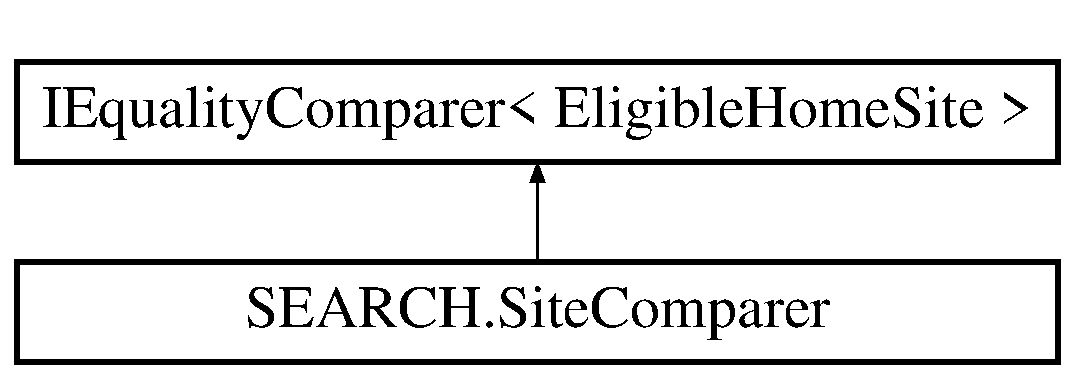
\includegraphics[height=2.000000cm]{class_s_e_a_r_c_h_1_1_site_comparer}
\end{center}
\end{figure}
\subsection*{Public Member Functions}
\begin{DoxyCompactItemize}
\item 
bool \hyperlink{class_s_e_a_r_c_h_1_1_site_comparer_a49775f035bf0e63bc85879bb21914e4d}{Equals} (\hyperlink{class_s_e_a_r_c_h_1_1_eligible_home_site}{Eligible\-Home\-Site} x, \hyperlink{class_s_e_a_r_c_h_1_1_eligible_home_site}{Eligible\-Home\-Site} y)
\item 
int \hyperlink{class_s_e_a_r_c_h_1_1_site_comparer_addc6d3810613eec71971cff161a3338e}{Get\-Hash\-Code} (\hyperlink{class_s_e_a_r_c_h_1_1_eligible_home_site}{Eligible\-Home\-Site} obj)
\end{DoxyCompactItemize}


\subsection{Member Function Documentation}
\hypertarget{class_s_e_a_r_c_h_1_1_site_comparer_a49775f035bf0e63bc85879bb21914e4d}{\index{S\-E\-A\-R\-C\-H\-::\-Site\-Comparer@{S\-E\-A\-R\-C\-H\-::\-Site\-Comparer}!Equals@{Equals}}
\index{Equals@{Equals}!SEARCH::SiteComparer@{S\-E\-A\-R\-C\-H\-::\-Site\-Comparer}}
\subsubsection[{Equals}]{\setlength{\rightskip}{0pt plus 5cm}bool S\-E\-A\-R\-C\-H.\-Site\-Comparer.\-Equals (
\begin{DoxyParamCaption}
\item[{{\bf Eligible\-Home\-Site}}]{x, }
\item[{{\bf Eligible\-Home\-Site}}]{y}
\end{DoxyParamCaption}
)}}\label{class_s_e_a_r_c_h_1_1_site_comparer_a49775f035bf0e63bc85879bb21914e4d}
\hypertarget{class_s_e_a_r_c_h_1_1_site_comparer_addc6d3810613eec71971cff161a3338e}{\index{S\-E\-A\-R\-C\-H\-::\-Site\-Comparer@{S\-E\-A\-R\-C\-H\-::\-Site\-Comparer}!Get\-Hash\-Code@{Get\-Hash\-Code}}
\index{Get\-Hash\-Code@{Get\-Hash\-Code}!SEARCH::SiteComparer@{S\-E\-A\-R\-C\-H\-::\-Site\-Comparer}}
\subsubsection[{Get\-Hash\-Code}]{\setlength{\rightskip}{0pt plus 5cm}int S\-E\-A\-R\-C\-H.\-Site\-Comparer.\-Get\-Hash\-Code (
\begin{DoxyParamCaption}
\item[{{\bf Eligible\-Home\-Site}}]{obj}
\end{DoxyParamCaption}
)}}\label{class_s_e_a_r_c_h_1_1_site_comparer_addc6d3810613eec71971cff161a3338e}


The documentation for this class was generated from the following file\-:\begin{DoxyCompactItemize}
\item 
Desktop/vlog4net\-A\-R\-C10\-\_\-64\-\_\-newhoming/\-Data\-Centric/\hyperlink{_eligible_home_site_8cs}{Eligible\-Home\-Site.\-cs}\end{DoxyCompactItemize}

\hypertarget{class_s_e_a_r_c_h_1_1_site_home_range_trigger}{\section{S\-E\-A\-R\-C\-H.\-Site\-Home\-Range\-Trigger Class Reference}
\label{class_s_e_a_r_c_h_1_1_site_home_range_trigger}\index{S\-E\-A\-R\-C\-H.\-Site\-Home\-Range\-Trigger@{S\-E\-A\-R\-C\-H.\-Site\-Home\-Range\-Trigger}}
}


Summary description for \hyperlink{class_s_e_a_r_c_h_1_1_site_home_range_trigger}{Site\-Home\-Range\-Trigger}.  


Inheritance diagram for S\-E\-A\-R\-C\-H.\-Site\-Home\-Range\-Trigger\-:\begin{figure}[H]
\begin{center}
\leavevmode
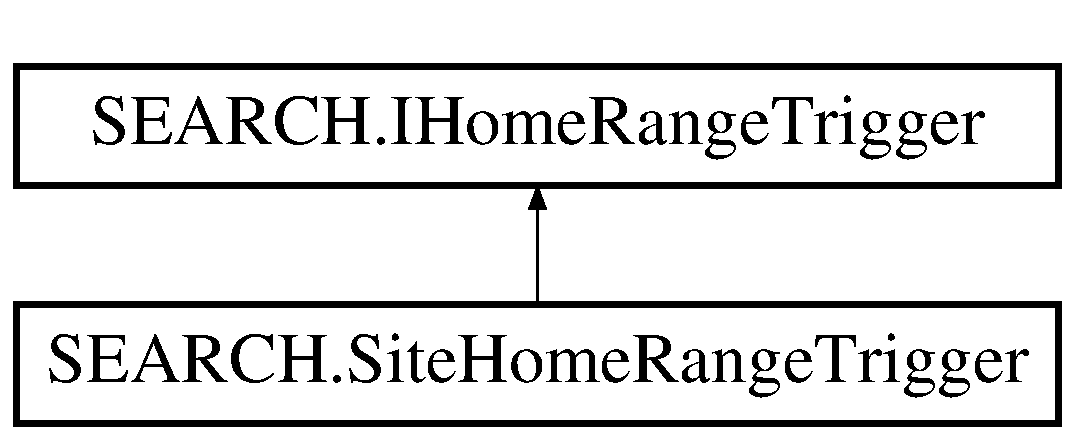
\includegraphics[height=2.000000cm]{class_s_e_a_r_c_h_1_1_site_home_range_trigger}
\end{center}
\end{figure}
\subsection*{Public Member Functions}
\begin{DoxyCompactItemize}
\item 
\hyperlink{class_s_e_a_r_c_h_1_1_site_home_range_trigger_a009fd626c855b60e4e0a56ecfd3865c7}{Site\-Home\-Range\-Trigger} (int \hyperlink{class_s_e_a_r_c_h_1_1_site_home_range_trigger_ac970fa3d8b811d475886681569e0929d}{num\-Times}, int in\-Num\-Animals)
\item 
void \hyperlink{class_s_e_a_r_c_h_1_1_site_home_range_trigger_a7266d98080f93ce4ad13e0b6ecfa805c}{reset} (int in\-Num\-Animals)
\item 
bool \hyperlink{class_s_e_a_r_c_h_1_1_site_home_range_trigger_a89af0390fd4719b591b674c4f9f60863}{time\-To\-Look\-For\-Home} (\hyperlink{class_s_e_a_r_c_h_1_1_animal}{Animal} in\-A)
\end{DoxyCompactItemize}
\subsection*{Properties}
\begin{DoxyCompactItemize}
\item 
int \hyperlink{class_s_e_a_r_c_h_1_1_site_home_range_trigger_ac970fa3d8b811d475886681569e0929d}{num\-Times}\hspace{0.3cm}{\ttfamily  \mbox{[}get, set\mbox{]}}
\end{DoxyCompactItemize}


\subsection{Detailed Description}
Summary description for \hyperlink{class_s_e_a_r_c_h_1_1_site_home_range_trigger}{Site\-Home\-Range\-Trigger}. 



\subsection{Constructor \& Destructor Documentation}
\hypertarget{class_s_e_a_r_c_h_1_1_site_home_range_trigger_a009fd626c855b60e4e0a56ecfd3865c7}{\index{S\-E\-A\-R\-C\-H\-::\-Site\-Home\-Range\-Trigger@{S\-E\-A\-R\-C\-H\-::\-Site\-Home\-Range\-Trigger}!Site\-Home\-Range\-Trigger@{Site\-Home\-Range\-Trigger}}
\index{Site\-Home\-Range\-Trigger@{Site\-Home\-Range\-Trigger}!SEARCH::SiteHomeRangeTrigger@{S\-E\-A\-R\-C\-H\-::\-Site\-Home\-Range\-Trigger}}
\subsubsection[{Site\-Home\-Range\-Trigger}]{\setlength{\rightskip}{0pt plus 5cm}S\-E\-A\-R\-C\-H.\-Site\-Home\-Range\-Trigger.\-Site\-Home\-Range\-Trigger (
\begin{DoxyParamCaption}
\item[{int}]{num\-Times, }
\item[{int}]{in\-Num\-Animals}
\end{DoxyParamCaption}
)}}\label{class_s_e_a_r_c_h_1_1_site_home_range_trigger_a009fd626c855b60e4e0a56ecfd3865c7}


\subsection{Member Function Documentation}
\hypertarget{class_s_e_a_r_c_h_1_1_site_home_range_trigger_a7266d98080f93ce4ad13e0b6ecfa805c}{\index{S\-E\-A\-R\-C\-H\-::\-Site\-Home\-Range\-Trigger@{S\-E\-A\-R\-C\-H\-::\-Site\-Home\-Range\-Trigger}!reset@{reset}}
\index{reset@{reset}!SEARCH::SiteHomeRangeTrigger@{S\-E\-A\-R\-C\-H\-::\-Site\-Home\-Range\-Trigger}}
\subsubsection[{reset}]{\setlength{\rightskip}{0pt plus 5cm}void S\-E\-A\-R\-C\-H.\-Site\-Home\-Range\-Trigger.\-reset (
\begin{DoxyParamCaption}
\item[{int}]{in\-Num\-Animals}
\end{DoxyParamCaption}
)}}\label{class_s_e_a_r_c_h_1_1_site_home_range_trigger_a7266d98080f93ce4ad13e0b6ecfa805c}


Implements \hyperlink{interface_s_e_a_r_c_h_1_1_i_home_range_trigger_a3d6cabe1057278e2c4369649254baea6}{S\-E\-A\-R\-C\-H.\-I\-Home\-Range\-Trigger}.

\hypertarget{class_s_e_a_r_c_h_1_1_site_home_range_trigger_a89af0390fd4719b591b674c4f9f60863}{\index{S\-E\-A\-R\-C\-H\-::\-Site\-Home\-Range\-Trigger@{S\-E\-A\-R\-C\-H\-::\-Site\-Home\-Range\-Trigger}!time\-To\-Look\-For\-Home@{time\-To\-Look\-For\-Home}}
\index{time\-To\-Look\-For\-Home@{time\-To\-Look\-For\-Home}!SEARCH::SiteHomeRangeTrigger@{S\-E\-A\-R\-C\-H\-::\-Site\-Home\-Range\-Trigger}}
\subsubsection[{time\-To\-Look\-For\-Home}]{\setlength{\rightskip}{0pt plus 5cm}bool S\-E\-A\-R\-C\-H.\-Site\-Home\-Range\-Trigger.\-time\-To\-Look\-For\-Home (
\begin{DoxyParamCaption}
\item[{{\bf Animal}}]{in\-A}
\end{DoxyParamCaption}
)}}\label{class_s_e_a_r_c_h_1_1_site_home_range_trigger_a89af0390fd4719b591b674c4f9f60863}


Implements \hyperlink{interface_s_e_a_r_c_h_1_1_i_home_range_trigger_ac7476deb63d55a92c635d2d4a479db4d}{S\-E\-A\-R\-C\-H.\-I\-Home\-Range\-Trigger}.



\subsection{Property Documentation}
\hypertarget{class_s_e_a_r_c_h_1_1_site_home_range_trigger_ac970fa3d8b811d475886681569e0929d}{\index{S\-E\-A\-R\-C\-H\-::\-Site\-Home\-Range\-Trigger@{S\-E\-A\-R\-C\-H\-::\-Site\-Home\-Range\-Trigger}!num\-Times@{num\-Times}}
\index{num\-Times@{num\-Times}!SEARCH::SiteHomeRangeTrigger@{S\-E\-A\-R\-C\-H\-::\-Site\-Home\-Range\-Trigger}}
\subsubsection[{num\-Times}]{\setlength{\rightskip}{0pt plus 5cm}int S\-E\-A\-R\-C\-H.\-Site\-Home\-Range\-Trigger.\-num\-Times\hspace{0.3cm}{\ttfamily [get]}, {\ttfamily [set]}}}\label{class_s_e_a_r_c_h_1_1_site_home_range_trigger_ac970fa3d8b811d475886681569e0929d}


The documentation for this class was generated from the following file\-:\begin{DoxyCompactItemize}
\item 
Desktop/vlog4net\-A\-R\-C10\-\_\-64\-\_\-newhoming/\-Data\-Centric/\hyperlink{_site_home_range_trigger_8cs}{Site\-Home\-Range\-Trigger.\-cs}\end{DoxyCompactItemize}

\hypertarget{class_s_e_a_r_c_h_1_1_sleep_mover}{\section{S\-E\-A\-R\-C\-H.\-Sleep\-Mover Class Reference}
\label{class_s_e_a_r_c_h_1_1_sleep_mover}\index{S\-E\-A\-R\-C\-H.\-Sleep\-Mover@{S\-E\-A\-R\-C\-H.\-Sleep\-Mover}}
}


 


Inheritance diagram for S\-E\-A\-R\-C\-H.\-Sleep\-Mover\-:\begin{figure}[H]
\begin{center}
\leavevmode
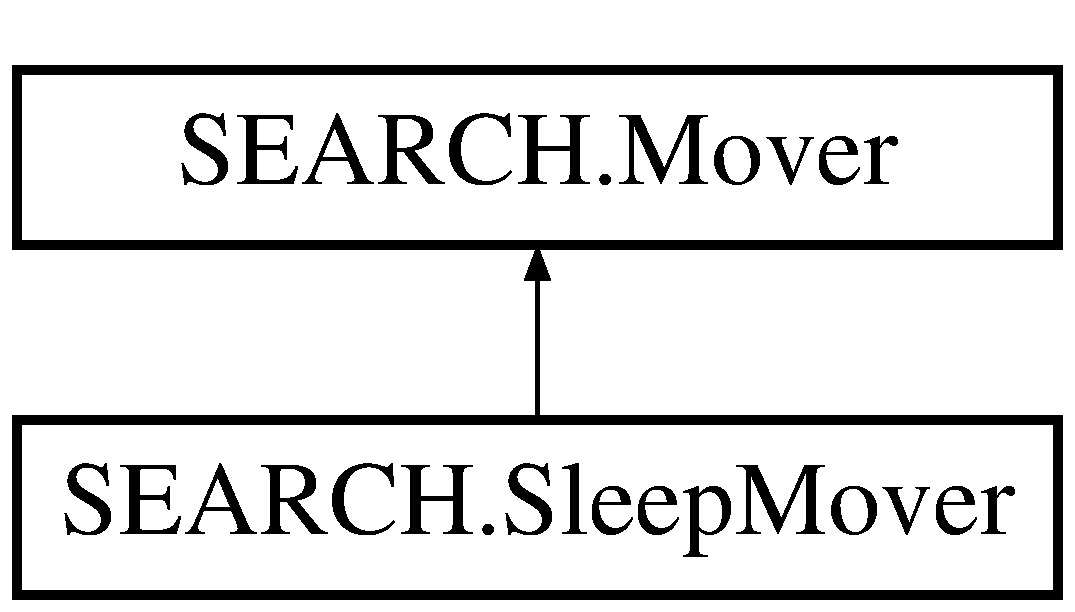
\includegraphics[height=2.000000cm]{class_s_e_a_r_c_h_1_1_sleep_mover}
\end{center}
\end{figure}
\subsection*{Public Member Functions}
\begin{DoxyCompactItemize}
\item 
override double \hyperlink{class_s_e_a_r_c_h_1_1_sleep_mover_a00e109927daf570d0c406339478131f9}{get\-Step\-Length} ()
\item 
override double \hyperlink{class_s_e_a_r_c_h_1_1_sleep_mover_a47d7e8dbf23341dd28383c9996d1b8c6}{get\-Turn\-Angle} (double rho)
\item 
override void \hyperlink{class_s_e_a_r_c_h_1_1_sleep_mover_a0bd6a7a748ebf84be7d7f209b395a8ce}{move} (ref double percent\-Time\-Step, \hyperlink{class_s_e_a_r_c_h_1_1_animal}{Animal} in\-A)
\end{DoxyCompactItemize}
\subsection*{Static Public Member Functions}
\begin{DoxyCompactItemize}
\item 
static \hyperlink{class_s_e_a_r_c_h_1_1_sleep_mover}{Sleep\-Mover} \hyperlink{class_s_e_a_r_c_h_1_1_sleep_mover_a2d2886842316b87f35e94c1a1e1a45bd}{get\-Sleep\-Mover} ()
\end{DoxyCompactItemize}
\subsection*{Additional Inherited Members}


\subsection{Detailed Description}




\subsection{Member Function Documentation}
\hypertarget{class_s_e_a_r_c_h_1_1_sleep_mover_a2d2886842316b87f35e94c1a1e1a45bd}{\index{S\-E\-A\-R\-C\-H\-::\-Sleep\-Mover@{S\-E\-A\-R\-C\-H\-::\-Sleep\-Mover}!get\-Sleep\-Mover@{get\-Sleep\-Mover}}
\index{get\-Sleep\-Mover@{get\-Sleep\-Mover}!SEARCH::SleepMover@{S\-E\-A\-R\-C\-H\-::\-Sleep\-Mover}}
\subsubsection[{get\-Sleep\-Mover}]{\setlength{\rightskip}{0pt plus 5cm}static {\bf Sleep\-Mover} S\-E\-A\-R\-C\-H.\-Sleep\-Mover.\-get\-Sleep\-Mover (
\begin{DoxyParamCaption}
{}
\end{DoxyParamCaption}
)\hspace{0.3cm}{\ttfamily [static]}}}\label{class_s_e_a_r_c_h_1_1_sleep_mover_a2d2886842316b87f35e94c1a1e1a45bd}
\hypertarget{class_s_e_a_r_c_h_1_1_sleep_mover_a00e109927daf570d0c406339478131f9}{\index{S\-E\-A\-R\-C\-H\-::\-Sleep\-Mover@{S\-E\-A\-R\-C\-H\-::\-Sleep\-Mover}!get\-Step\-Length@{get\-Step\-Length}}
\index{get\-Step\-Length@{get\-Step\-Length}!SEARCH::SleepMover@{S\-E\-A\-R\-C\-H\-::\-Sleep\-Mover}}
\subsubsection[{get\-Step\-Length}]{\setlength{\rightskip}{0pt plus 5cm}override double S\-E\-A\-R\-C\-H.\-Sleep\-Mover.\-get\-Step\-Length (
\begin{DoxyParamCaption}
{}
\end{DoxyParamCaption}
)\hspace{0.3cm}{\ttfamily [virtual]}}}\label{class_s_e_a_r_c_h_1_1_sleep_mover_a00e109927daf570d0c406339478131f9}


Implements \hyperlink{class_s_e_a_r_c_h_1_1_mover_a3e547800bbc34492f4251adee70dbf02}{S\-E\-A\-R\-C\-H.\-Mover}.

\hypertarget{class_s_e_a_r_c_h_1_1_sleep_mover_a47d7e8dbf23341dd28383c9996d1b8c6}{\index{S\-E\-A\-R\-C\-H\-::\-Sleep\-Mover@{S\-E\-A\-R\-C\-H\-::\-Sleep\-Mover}!get\-Turn\-Angle@{get\-Turn\-Angle}}
\index{get\-Turn\-Angle@{get\-Turn\-Angle}!SEARCH::SleepMover@{S\-E\-A\-R\-C\-H\-::\-Sleep\-Mover}}
\subsubsection[{get\-Turn\-Angle}]{\setlength{\rightskip}{0pt plus 5cm}override double S\-E\-A\-R\-C\-H.\-Sleep\-Mover.\-get\-Turn\-Angle (
\begin{DoxyParamCaption}
\item[{double}]{rho}
\end{DoxyParamCaption}
)\hspace{0.3cm}{\ttfamily [virtual]}}}\label{class_s_e_a_r_c_h_1_1_sleep_mover_a47d7e8dbf23341dd28383c9996d1b8c6}


Implements \hyperlink{class_s_e_a_r_c_h_1_1_mover_a879a44d5a0c57434375a69c8d8d00e35}{S\-E\-A\-R\-C\-H.\-Mover}.

\hypertarget{class_s_e_a_r_c_h_1_1_sleep_mover_a0bd6a7a748ebf84be7d7f209b395a8ce}{\index{S\-E\-A\-R\-C\-H\-::\-Sleep\-Mover@{S\-E\-A\-R\-C\-H\-::\-Sleep\-Mover}!move@{move}}
\index{move@{move}!SEARCH::SleepMover@{S\-E\-A\-R\-C\-H\-::\-Sleep\-Mover}}
\subsubsection[{move}]{\setlength{\rightskip}{0pt plus 5cm}override void S\-E\-A\-R\-C\-H.\-Sleep\-Mover.\-move (
\begin{DoxyParamCaption}
\item[{ref double}]{percent\-Time\-Step, }
\item[{{\bf Animal}}]{in\-A}
\end{DoxyParamCaption}
)\hspace{0.3cm}{\ttfamily [virtual]}}}\label{class_s_e_a_r_c_h_1_1_sleep_mover_a0bd6a7a748ebf84be7d7f209b395a8ce}


Reimplemented from \hyperlink{class_s_e_a_r_c_h_1_1_mover_ab2dfc659f3817ea48d66ff4d7e464d1d}{S\-E\-A\-R\-C\-H.\-Mover}.



The documentation for this class was generated from the following file\-:\begin{DoxyCompactItemize}
\item 
Desktop/vlog4net\-A\-R\-C10\-\_\-64\-\_\-newhoming/\-Data\-Centric/\hyperlink{_sleep_mover_8cs}{Sleep\-Mover.\-cs}\end{DoxyCompactItemize}

\hypertarget{class_s_e_a_r_c_h_1_1_straight_mover}{\section{S\-E\-A\-R\-C\-H.\-Straight\-Mover Class Reference}
\label{class_s_e_a_r_c_h_1_1_straight_mover}\index{S\-E\-A\-R\-C\-H.\-Straight\-Mover@{S\-E\-A\-R\-C\-H.\-Straight\-Mover}}
}


Summary description for \hyperlink{class_s_e_a_r_c_h_1_1_straight_mover}{Straight\-Mover}.  


Inheritance diagram for S\-E\-A\-R\-C\-H.\-Straight\-Mover\-:\begin{figure}[H]
\begin{center}
\leavevmode
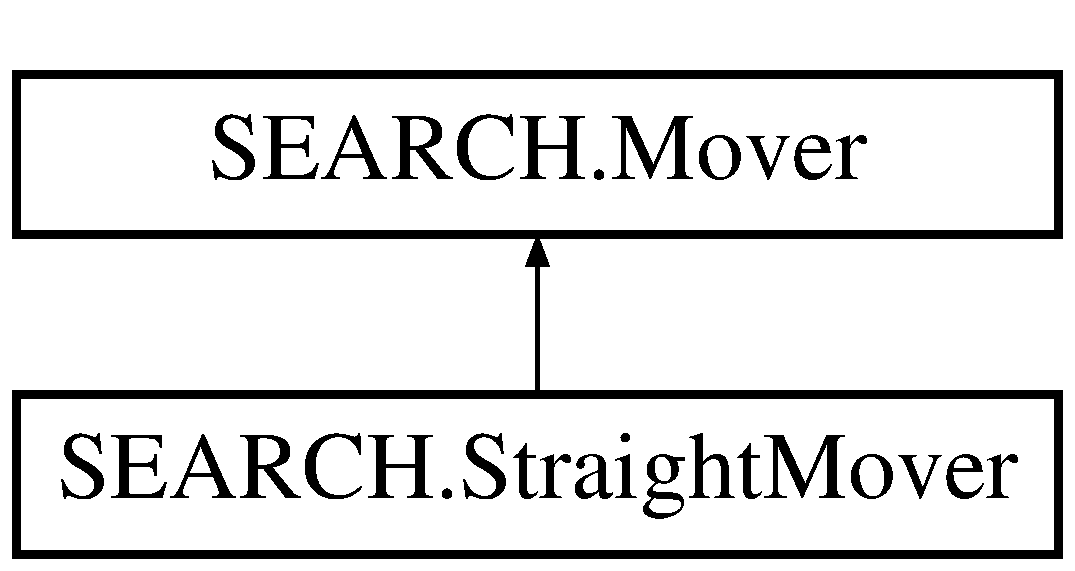
\includegraphics[height=2.000000cm]{class_s_e_a_r_c_h_1_1_straight_mover}
\end{center}
\end{figure}
\subsection*{Public Member Functions}
\begin{DoxyCompactItemize}
\item 
override double \hyperlink{class_s_e_a_r_c_h_1_1_straight_mover_a146501b931a5784a3b68f7251048729f}{get\-Step\-Length} ()
\item 
override double \hyperlink{class_s_e_a_r_c_h_1_1_straight_mover_ad40a2a1e1e3103786928f7be8c30d5b1}{get\-Turn\-Angle} (double rho)
\end{DoxyCompactItemize}
\subsection*{Static Public Member Functions}
\begin{DoxyCompactItemize}
\item 
static \hyperlink{class_s_e_a_r_c_h_1_1_straight_mover}{Straight\-Mover} \hyperlink{class_s_e_a_r_c_h_1_1_straight_mover_acc3ba639a92903e9cfdaaa00d10d266b}{get\-Straight\-Mover} ()
\end{DoxyCompactItemize}
\subsection*{Additional Inherited Members}


\subsection{Detailed Description}
Summary description for \hyperlink{class_s_e_a_r_c_h_1_1_straight_mover}{Straight\-Mover}. 



\subsection{Member Function Documentation}
\hypertarget{class_s_e_a_r_c_h_1_1_straight_mover_a146501b931a5784a3b68f7251048729f}{\index{S\-E\-A\-R\-C\-H\-::\-Straight\-Mover@{S\-E\-A\-R\-C\-H\-::\-Straight\-Mover}!get\-Step\-Length@{get\-Step\-Length}}
\index{get\-Step\-Length@{get\-Step\-Length}!SEARCH::StraightMover@{S\-E\-A\-R\-C\-H\-::\-Straight\-Mover}}
\subsubsection[{get\-Step\-Length}]{\setlength{\rightskip}{0pt plus 5cm}override double S\-E\-A\-R\-C\-H.\-Straight\-Mover.\-get\-Step\-Length (
\begin{DoxyParamCaption}
{}
\end{DoxyParamCaption}
)\hspace{0.3cm}{\ttfamily [virtual]}}}\label{class_s_e_a_r_c_h_1_1_straight_mover_a146501b931a5784a3b68f7251048729f}


Implements \hyperlink{class_s_e_a_r_c_h_1_1_mover_a3e547800bbc34492f4251adee70dbf02}{S\-E\-A\-R\-C\-H.\-Mover}.

\hypertarget{class_s_e_a_r_c_h_1_1_straight_mover_acc3ba639a92903e9cfdaaa00d10d266b}{\index{S\-E\-A\-R\-C\-H\-::\-Straight\-Mover@{S\-E\-A\-R\-C\-H\-::\-Straight\-Mover}!get\-Straight\-Mover@{get\-Straight\-Mover}}
\index{get\-Straight\-Mover@{get\-Straight\-Mover}!SEARCH::StraightMover@{S\-E\-A\-R\-C\-H\-::\-Straight\-Mover}}
\subsubsection[{get\-Straight\-Mover}]{\setlength{\rightskip}{0pt plus 5cm}static {\bf Straight\-Mover} S\-E\-A\-R\-C\-H.\-Straight\-Mover.\-get\-Straight\-Mover (
\begin{DoxyParamCaption}
{}
\end{DoxyParamCaption}
)\hspace{0.3cm}{\ttfamily [static]}}}\label{class_s_e_a_r_c_h_1_1_straight_mover_acc3ba639a92903e9cfdaaa00d10d266b}
\hypertarget{class_s_e_a_r_c_h_1_1_straight_mover_ad40a2a1e1e3103786928f7be8c30d5b1}{\index{S\-E\-A\-R\-C\-H\-::\-Straight\-Mover@{S\-E\-A\-R\-C\-H\-::\-Straight\-Mover}!get\-Turn\-Angle@{get\-Turn\-Angle}}
\index{get\-Turn\-Angle@{get\-Turn\-Angle}!SEARCH::StraightMover@{S\-E\-A\-R\-C\-H\-::\-Straight\-Mover}}
\subsubsection[{get\-Turn\-Angle}]{\setlength{\rightskip}{0pt plus 5cm}override double S\-E\-A\-R\-C\-H.\-Straight\-Mover.\-get\-Turn\-Angle (
\begin{DoxyParamCaption}
\item[{double}]{rho}
\end{DoxyParamCaption}
)\hspace{0.3cm}{\ttfamily [virtual]}}}\label{class_s_e_a_r_c_h_1_1_straight_mover_ad40a2a1e1e3103786928f7be8c30d5b1}


Implements \hyperlink{class_s_e_a_r_c_h_1_1_mover_a879a44d5a0c57434375a69c8d8d00e35}{S\-E\-A\-R\-C\-H.\-Mover}.



The documentation for this class was generated from the following file\-:\begin{DoxyCompactItemize}
\item 
Desktop/vlog4net\-A\-R\-C10\-\_\-64\-\_\-newhoming/\-Data\-Centric/\hyperlink{_straight_mover_8cs}{Straight\-Mover.\-cs}\end{DoxyCompactItemize}

\hypertarget{class_s_e_a_r_c_h_1_1_temporal_modifiers}{\section{S\-E\-A\-R\-C\-H.\-Temporal\-Modifiers Class Reference}
\label{class_s_e_a_r_c_h_1_1_temporal_modifiers}\index{S\-E\-A\-R\-C\-H.\-Temporal\-Modifiers@{S\-E\-A\-R\-C\-H.\-Temporal\-Modifiers}}
}
\subsection*{Public Attributes}
\begin{DoxyCompactItemize}
\item 
int \hyperlink{class_s_e_a_r_c_h_1_1_temporal_modifiers_a792b00d4d518565252aa4963fd7595c4}{body\-Fat\-Reduction}
\item 
int \hyperlink{class_s_e_a_r_c_h_1_1_temporal_modifiers_a1b1d7d01c542f6b45fd1be5944fc0483}{capture\-Food}
\item 
int \hyperlink{class_s_e_a_r_c_h_1_1_temporal_modifiers_ab2ee566ad9f28ff631cb5384d3da0e45}{move\-Speed}
\item 
int \hyperlink{class_s_e_a_r_c_h_1_1_temporal_modifiers_aa290e2008609fd0568b1224cac3e2af5}{move\-Turtosity}
\item 
int \hyperlink{class_s_e_a_r_c_h_1_1_temporal_modifiers_afb6549fda216fb9ad82f311e4db2813e}{percepton\-Modifier}
\item 
int \hyperlink{class_s_e_a_r_c_h_1_1_temporal_modifiers_a28bc2a746df06ddf74ac9cc5946564fc}{predation\-Risk}
\end{DoxyCompactItemize}


\subsection{Member Data Documentation}
\hypertarget{class_s_e_a_r_c_h_1_1_temporal_modifiers_a792b00d4d518565252aa4963fd7595c4}{\index{S\-E\-A\-R\-C\-H\-::\-Temporal\-Modifiers@{S\-E\-A\-R\-C\-H\-::\-Temporal\-Modifiers}!body\-Fat\-Reduction@{body\-Fat\-Reduction}}
\index{body\-Fat\-Reduction@{body\-Fat\-Reduction}!SEARCH::TemporalModifiers@{S\-E\-A\-R\-C\-H\-::\-Temporal\-Modifiers}}
\subsubsection[{body\-Fat\-Reduction}]{\setlength{\rightskip}{0pt plus 5cm}int S\-E\-A\-R\-C\-H.\-Temporal\-Modifiers.\-body\-Fat\-Reduction}}\label{class_s_e_a_r_c_h_1_1_temporal_modifiers_a792b00d4d518565252aa4963fd7595c4}
\hypertarget{class_s_e_a_r_c_h_1_1_temporal_modifiers_a1b1d7d01c542f6b45fd1be5944fc0483}{\index{S\-E\-A\-R\-C\-H\-::\-Temporal\-Modifiers@{S\-E\-A\-R\-C\-H\-::\-Temporal\-Modifiers}!capture\-Food@{capture\-Food}}
\index{capture\-Food@{capture\-Food}!SEARCH::TemporalModifiers@{S\-E\-A\-R\-C\-H\-::\-Temporal\-Modifiers}}
\subsubsection[{capture\-Food}]{\setlength{\rightskip}{0pt plus 5cm}int S\-E\-A\-R\-C\-H.\-Temporal\-Modifiers.\-capture\-Food}}\label{class_s_e_a_r_c_h_1_1_temporal_modifiers_a1b1d7d01c542f6b45fd1be5944fc0483}
\hypertarget{class_s_e_a_r_c_h_1_1_temporal_modifiers_ab2ee566ad9f28ff631cb5384d3da0e45}{\index{S\-E\-A\-R\-C\-H\-::\-Temporal\-Modifiers@{S\-E\-A\-R\-C\-H\-::\-Temporal\-Modifiers}!move\-Speed@{move\-Speed}}
\index{move\-Speed@{move\-Speed}!SEARCH::TemporalModifiers@{S\-E\-A\-R\-C\-H\-::\-Temporal\-Modifiers}}
\subsubsection[{move\-Speed}]{\setlength{\rightskip}{0pt plus 5cm}int S\-E\-A\-R\-C\-H.\-Temporal\-Modifiers.\-move\-Speed}}\label{class_s_e_a_r_c_h_1_1_temporal_modifiers_ab2ee566ad9f28ff631cb5384d3da0e45}
\hypertarget{class_s_e_a_r_c_h_1_1_temporal_modifiers_aa290e2008609fd0568b1224cac3e2af5}{\index{S\-E\-A\-R\-C\-H\-::\-Temporal\-Modifiers@{S\-E\-A\-R\-C\-H\-::\-Temporal\-Modifiers}!move\-Turtosity@{move\-Turtosity}}
\index{move\-Turtosity@{move\-Turtosity}!SEARCH::TemporalModifiers@{S\-E\-A\-R\-C\-H\-::\-Temporal\-Modifiers}}
\subsubsection[{move\-Turtosity}]{\setlength{\rightskip}{0pt plus 5cm}int S\-E\-A\-R\-C\-H.\-Temporal\-Modifiers.\-move\-Turtosity}}\label{class_s_e_a_r_c_h_1_1_temporal_modifiers_aa290e2008609fd0568b1224cac3e2af5}
\hypertarget{class_s_e_a_r_c_h_1_1_temporal_modifiers_afb6549fda216fb9ad82f311e4db2813e}{\index{S\-E\-A\-R\-C\-H\-::\-Temporal\-Modifiers@{S\-E\-A\-R\-C\-H\-::\-Temporal\-Modifiers}!percepton\-Modifier@{percepton\-Modifier}}
\index{percepton\-Modifier@{percepton\-Modifier}!SEARCH::TemporalModifiers@{S\-E\-A\-R\-C\-H\-::\-Temporal\-Modifiers}}
\subsubsection[{percepton\-Modifier}]{\setlength{\rightskip}{0pt plus 5cm}int S\-E\-A\-R\-C\-H.\-Temporal\-Modifiers.\-percepton\-Modifier}}\label{class_s_e_a_r_c_h_1_1_temporal_modifiers_afb6549fda216fb9ad82f311e4db2813e}
\hypertarget{class_s_e_a_r_c_h_1_1_temporal_modifiers_a28bc2a746df06ddf74ac9cc5946564fc}{\index{S\-E\-A\-R\-C\-H\-::\-Temporal\-Modifiers@{S\-E\-A\-R\-C\-H\-::\-Temporal\-Modifiers}!predation\-Risk@{predation\-Risk}}
\index{predation\-Risk@{predation\-Risk}!SEARCH::TemporalModifiers@{S\-E\-A\-R\-C\-H\-::\-Temporal\-Modifiers}}
\subsubsection[{predation\-Risk}]{\setlength{\rightskip}{0pt plus 5cm}int S\-E\-A\-R\-C\-H.\-Temporal\-Modifiers.\-predation\-Risk}}\label{class_s_e_a_r_c_h_1_1_temporal_modifiers_a28bc2a746df06ddf74ac9cc5946564fc}


The documentation for this class was generated from the following file\-:\begin{DoxyCompactItemize}
\item 
Desktop/vlog4net\-A\-R\-C10\-\_\-64\-\_\-newhoming/\-Data\-Centric/\hyperlink{_temporal_modifiers_8cs}{Temporal\-Modifiers.\-cs}\end{DoxyCompactItemize}

\hypertarget{class_s_e_a_r_c_h_1_1_text_file_writer}{\section{S\-E\-A\-R\-C\-H.\-Text\-File\-Writer Class Reference}
\label{class_s_e_a_r_c_h_1_1_text_file_writer}\index{S\-E\-A\-R\-C\-H.\-Text\-File\-Writer@{S\-E\-A\-R\-C\-H.\-Text\-File\-Writer}}
}
\subsection*{Public Member Functions}
\begin{DoxyCompactItemize}
\item 
\hyperlink{class_s_e_a_r_c_h_1_1_text_file_writer_a20c7535ef3d6c2de3a5cba015c3a56eb}{Text\-File\-Writer} (string path, string file\-Name)
\item 
void \hyperlink{class_s_e_a_r_c_h_1_1_text_file_writer_ae908042dbf7a37fc4928e850eaeebc78}{add\-Line} (string in\-Value)
\item 
void \hyperlink{class_s_e_a_r_c_h_1_1_text_file_writer_ad43e387f746f356bf693104e69e9015d}{close} ()
\item 
void \hyperlink{class_s_e_a_r_c_h_1_1_text_file_writer_a814f2b9f77612f7816c7c593a9395d60}{Write\-Out\-Time\-Step} ()
\end{DoxyCompactItemize}
\subsection*{Properties}
\begin{DoxyCompactItemize}
\item 
string \hyperlink{class_s_e_a_r_c_h_1_1_text_file_writer_a1de45f2a27a5bfacaaaeff639368b560}{Out\-Path}\hspace{0.3cm}{\ttfamily  \mbox{[}get, set\mbox{]}}
\end{DoxyCompactItemize}


\subsection{Constructor \& Destructor Documentation}
\hypertarget{class_s_e_a_r_c_h_1_1_text_file_writer_a20c7535ef3d6c2de3a5cba015c3a56eb}{\index{S\-E\-A\-R\-C\-H\-::\-Text\-File\-Writer@{S\-E\-A\-R\-C\-H\-::\-Text\-File\-Writer}!Text\-File\-Writer@{Text\-File\-Writer}}
\index{Text\-File\-Writer@{Text\-File\-Writer}!SEARCH::TextFileWriter@{S\-E\-A\-R\-C\-H\-::\-Text\-File\-Writer}}
\subsubsection[{Text\-File\-Writer}]{\setlength{\rightskip}{0pt plus 5cm}S\-E\-A\-R\-C\-H.\-Text\-File\-Writer.\-Text\-File\-Writer (
\begin{DoxyParamCaption}
\item[{string}]{path, }
\item[{string}]{file\-Name}
\end{DoxyParamCaption}
)}}\label{class_s_e_a_r_c_h_1_1_text_file_writer_a20c7535ef3d6c2de3a5cba015c3a56eb}


\subsection{Member Function Documentation}
\hypertarget{class_s_e_a_r_c_h_1_1_text_file_writer_ae908042dbf7a37fc4928e850eaeebc78}{\index{S\-E\-A\-R\-C\-H\-::\-Text\-File\-Writer@{S\-E\-A\-R\-C\-H\-::\-Text\-File\-Writer}!add\-Line@{add\-Line}}
\index{add\-Line@{add\-Line}!SEARCH::TextFileWriter@{S\-E\-A\-R\-C\-H\-::\-Text\-File\-Writer}}
\subsubsection[{add\-Line}]{\setlength{\rightskip}{0pt plus 5cm}void S\-E\-A\-R\-C\-H.\-Text\-File\-Writer.\-add\-Line (
\begin{DoxyParamCaption}
\item[{string}]{in\-Value}
\end{DoxyParamCaption}
)}}\label{class_s_e_a_r_c_h_1_1_text_file_writer_ae908042dbf7a37fc4928e850eaeebc78}
\hypertarget{class_s_e_a_r_c_h_1_1_text_file_writer_ad43e387f746f356bf693104e69e9015d}{\index{S\-E\-A\-R\-C\-H\-::\-Text\-File\-Writer@{S\-E\-A\-R\-C\-H\-::\-Text\-File\-Writer}!close@{close}}
\index{close@{close}!SEARCH::TextFileWriter@{S\-E\-A\-R\-C\-H\-::\-Text\-File\-Writer}}
\subsubsection[{close}]{\setlength{\rightskip}{0pt plus 5cm}void S\-E\-A\-R\-C\-H.\-Text\-File\-Writer.\-close (
\begin{DoxyParamCaption}
{}
\end{DoxyParamCaption}
)}}\label{class_s_e_a_r_c_h_1_1_text_file_writer_ad43e387f746f356bf693104e69e9015d}
\hypertarget{class_s_e_a_r_c_h_1_1_text_file_writer_a814f2b9f77612f7816c7c593a9395d60}{\index{S\-E\-A\-R\-C\-H\-::\-Text\-File\-Writer@{S\-E\-A\-R\-C\-H\-::\-Text\-File\-Writer}!Write\-Out\-Time\-Step@{Write\-Out\-Time\-Step}}
\index{Write\-Out\-Time\-Step@{Write\-Out\-Time\-Step}!SEARCH::TextFileWriter@{S\-E\-A\-R\-C\-H\-::\-Text\-File\-Writer}}
\subsubsection[{Write\-Out\-Time\-Step}]{\setlength{\rightskip}{0pt plus 5cm}void S\-E\-A\-R\-C\-H.\-Text\-File\-Writer.\-Write\-Out\-Time\-Step (
\begin{DoxyParamCaption}
{}
\end{DoxyParamCaption}
)}}\label{class_s_e_a_r_c_h_1_1_text_file_writer_a814f2b9f77612f7816c7c593a9395d60}


\subsection{Property Documentation}
\hypertarget{class_s_e_a_r_c_h_1_1_text_file_writer_a1de45f2a27a5bfacaaaeff639368b560}{\index{S\-E\-A\-R\-C\-H\-::\-Text\-File\-Writer@{S\-E\-A\-R\-C\-H\-::\-Text\-File\-Writer}!Out\-Path@{Out\-Path}}
\index{Out\-Path@{Out\-Path}!SEARCH::TextFileWriter@{S\-E\-A\-R\-C\-H\-::\-Text\-File\-Writer}}
\subsubsection[{Out\-Path}]{\setlength{\rightskip}{0pt plus 5cm}string S\-E\-A\-R\-C\-H.\-Text\-File\-Writer.\-Out\-Path\hspace{0.3cm}{\ttfamily [get]}, {\ttfamily [set]}}}\label{class_s_e_a_r_c_h_1_1_text_file_writer_a1de45f2a27a5bfacaaaeff639368b560}


The documentation for this class was generated from the following file\-:\begin{DoxyCompactItemize}
\item 
Desktop/vlog4net\-A\-R\-C10\-\_\-64\-\_\-newhoming/\-Data\-Centric/\hyperlink{_text_file_writer_8cs}{Text\-File\-Writer.\-cs}\end{DoxyCompactItemize}

\hypertarget{class_s_e_a_r_c_h_1_1_time_home_range_trigger}{\section{S\-E\-A\-R\-C\-H.\-Time\-Home\-Range\-Trigger Class Reference}
\label{class_s_e_a_r_c_h_1_1_time_home_range_trigger}\index{S\-E\-A\-R\-C\-H.\-Time\-Home\-Range\-Trigger@{S\-E\-A\-R\-C\-H.\-Time\-Home\-Range\-Trigger}}
}
Inheritance diagram for S\-E\-A\-R\-C\-H.\-Time\-Home\-Range\-Trigger\-:\begin{figure}[H]
\begin{center}
\leavevmode
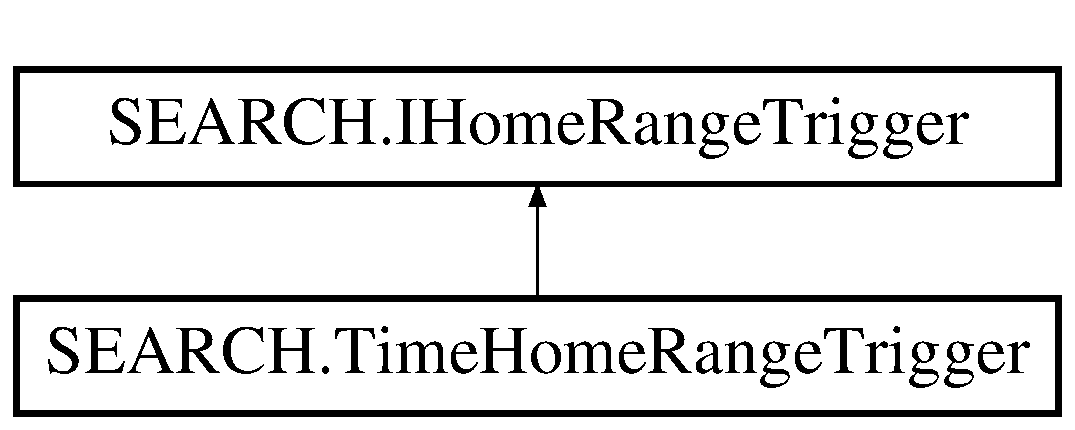
\includegraphics[height=2.000000cm]{class_s_e_a_r_c_h_1_1_time_home_range_trigger}
\end{center}
\end{figure}
\subsection*{Public Member Functions}
\begin{DoxyCompactItemize}
\item 
\hyperlink{class_s_e_a_r_c_h_1_1_time_home_range_trigger_ab1c4a4a353c96ddb3c1ef68b7204ba29}{Time\-Home\-Range\-Trigger} (int \hyperlink{class_s_e_a_r_c_h_1_1_time_home_range_trigger_aac2658cafbac6f2827bbf64d69df3481}{num\-Times}, int num\-Animals)
\item 
void \hyperlink{class_s_e_a_r_c_h_1_1_time_home_range_trigger_afd1bace9c699ecf623e4ee72596873e4}{reset} (int num\-Animals)
\item 
bool \hyperlink{class_s_e_a_r_c_h_1_1_time_home_range_trigger_ad480f427e0e81b0331efd1e393b3dd65}{time\-To\-Look\-For\-Home} (\hyperlink{class_s_e_a_r_c_h_1_1_animal}{Animal} in\-A)
\end{DoxyCompactItemize}
\subsection*{Properties}
\begin{DoxyCompactItemize}
\item 
int \hyperlink{class_s_e_a_r_c_h_1_1_time_home_range_trigger_aac2658cafbac6f2827bbf64d69df3481}{num\-Times}\hspace{0.3cm}{\ttfamily  \mbox{[}get, set\mbox{]}}
\end{DoxyCompactItemize}


\subsection{Constructor \& Destructor Documentation}
\hypertarget{class_s_e_a_r_c_h_1_1_time_home_range_trigger_ab1c4a4a353c96ddb3c1ef68b7204ba29}{\index{S\-E\-A\-R\-C\-H\-::\-Time\-Home\-Range\-Trigger@{S\-E\-A\-R\-C\-H\-::\-Time\-Home\-Range\-Trigger}!Time\-Home\-Range\-Trigger@{Time\-Home\-Range\-Trigger}}
\index{Time\-Home\-Range\-Trigger@{Time\-Home\-Range\-Trigger}!SEARCH::TimeHomeRangeTrigger@{S\-E\-A\-R\-C\-H\-::\-Time\-Home\-Range\-Trigger}}
\subsubsection[{Time\-Home\-Range\-Trigger}]{\setlength{\rightskip}{0pt plus 5cm}S\-E\-A\-R\-C\-H.\-Time\-Home\-Range\-Trigger.\-Time\-Home\-Range\-Trigger (
\begin{DoxyParamCaption}
\item[{int}]{num\-Times, }
\item[{int}]{num\-Animals}
\end{DoxyParamCaption}
)}}\label{class_s_e_a_r_c_h_1_1_time_home_range_trigger_ab1c4a4a353c96ddb3c1ef68b7204ba29}


\subsection{Member Function Documentation}
\hypertarget{class_s_e_a_r_c_h_1_1_time_home_range_trigger_afd1bace9c699ecf623e4ee72596873e4}{\index{S\-E\-A\-R\-C\-H\-::\-Time\-Home\-Range\-Trigger@{S\-E\-A\-R\-C\-H\-::\-Time\-Home\-Range\-Trigger}!reset@{reset}}
\index{reset@{reset}!SEARCH::TimeHomeRangeTrigger@{S\-E\-A\-R\-C\-H\-::\-Time\-Home\-Range\-Trigger}}
\subsubsection[{reset}]{\setlength{\rightskip}{0pt plus 5cm}void S\-E\-A\-R\-C\-H.\-Time\-Home\-Range\-Trigger.\-reset (
\begin{DoxyParamCaption}
\item[{int}]{num\-Animals}
\end{DoxyParamCaption}
)}}\label{class_s_e_a_r_c_h_1_1_time_home_range_trigger_afd1bace9c699ecf623e4ee72596873e4}


Implements \hyperlink{interface_s_e_a_r_c_h_1_1_i_home_range_trigger_a3d6cabe1057278e2c4369649254baea6}{S\-E\-A\-R\-C\-H.\-I\-Home\-Range\-Trigger}.

\hypertarget{class_s_e_a_r_c_h_1_1_time_home_range_trigger_ad480f427e0e81b0331efd1e393b3dd65}{\index{S\-E\-A\-R\-C\-H\-::\-Time\-Home\-Range\-Trigger@{S\-E\-A\-R\-C\-H\-::\-Time\-Home\-Range\-Trigger}!time\-To\-Look\-For\-Home@{time\-To\-Look\-For\-Home}}
\index{time\-To\-Look\-For\-Home@{time\-To\-Look\-For\-Home}!SEARCH::TimeHomeRangeTrigger@{S\-E\-A\-R\-C\-H\-::\-Time\-Home\-Range\-Trigger}}
\subsubsection[{time\-To\-Look\-For\-Home}]{\setlength{\rightskip}{0pt plus 5cm}bool S\-E\-A\-R\-C\-H.\-Time\-Home\-Range\-Trigger.\-time\-To\-Look\-For\-Home (
\begin{DoxyParamCaption}
\item[{{\bf Animal}}]{in\-A}
\end{DoxyParamCaption}
)}}\label{class_s_e_a_r_c_h_1_1_time_home_range_trigger_ad480f427e0e81b0331efd1e393b3dd65}


Implements \hyperlink{interface_s_e_a_r_c_h_1_1_i_home_range_trigger_ac7476deb63d55a92c635d2d4a479db4d}{S\-E\-A\-R\-C\-H.\-I\-Home\-Range\-Trigger}.



\subsection{Property Documentation}
\hypertarget{class_s_e_a_r_c_h_1_1_time_home_range_trigger_aac2658cafbac6f2827bbf64d69df3481}{\index{S\-E\-A\-R\-C\-H\-::\-Time\-Home\-Range\-Trigger@{S\-E\-A\-R\-C\-H\-::\-Time\-Home\-Range\-Trigger}!num\-Times@{num\-Times}}
\index{num\-Times@{num\-Times}!SEARCH::TimeHomeRangeTrigger@{S\-E\-A\-R\-C\-H\-::\-Time\-Home\-Range\-Trigger}}
\subsubsection[{num\-Times}]{\setlength{\rightskip}{0pt plus 5cm}int S\-E\-A\-R\-C\-H.\-Time\-Home\-Range\-Trigger.\-num\-Times\hspace{0.3cm}{\ttfamily [get]}, {\ttfamily [set]}}}\label{class_s_e_a_r_c_h_1_1_time_home_range_trigger_aac2658cafbac6f2827bbf64d69df3481}


The documentation for this class was generated from the following file\-:\begin{DoxyCompactItemize}
\item 
Desktop/vlog4net\-A\-R\-C10\-\_\-64\-\_\-newhoming/\-Data\-Centric/\hyperlink{_time_home_range_trigger_8cs}{Time\-Home\-Range\-Trigger.\-cs}\end{DoxyCompactItemize}

\hypertarget{class_s_e_a_r_c_h_1_1_yearly_form}{\section{S\-E\-A\-R\-C\-H.\-Yearly\-Form Class Reference}
\label{class_s_e_a_r_c_h_1_1_yearly_form}\index{S\-E\-A\-R\-C\-H.\-Yearly\-Form@{S\-E\-A\-R\-C\-H.\-Yearly\-Form}}
}


Summary description for \hyperlink{class_s_e_a_r_c_h_1_1_yearly_form}{Yearly\-Form}.  


Inheritance diagram for S\-E\-A\-R\-C\-H.\-Yearly\-Form\-:\begin{figure}[H]
\begin{center}
\leavevmode
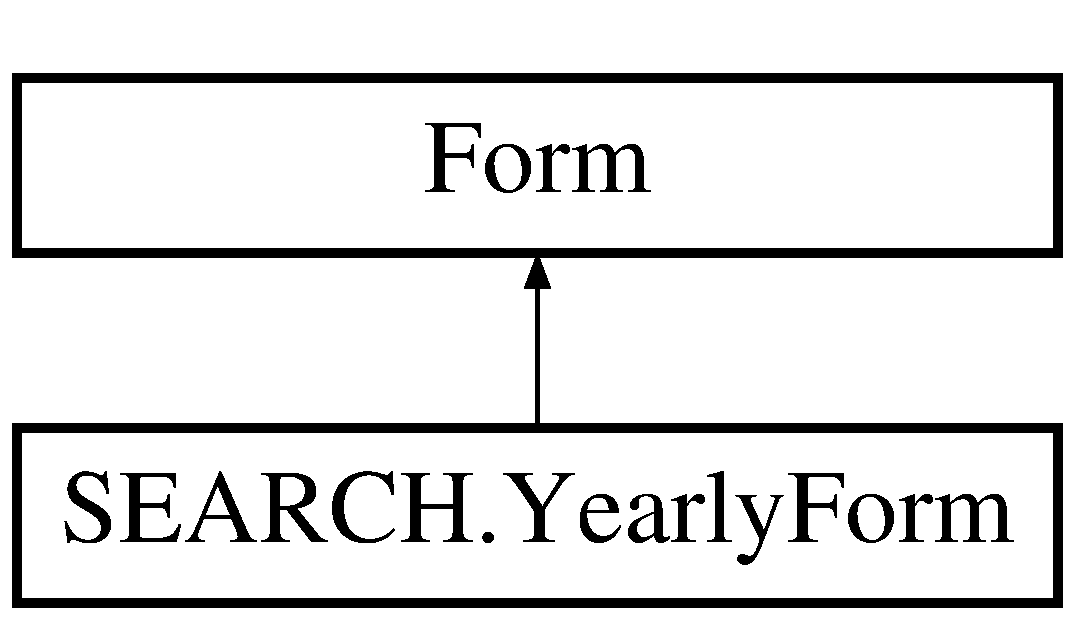
\includegraphics[height=2.000000cm]{class_s_e_a_r_c_h_1_1_yearly_form}
\end{center}
\end{figure}
\subsection*{Public Member Functions}
\begin{DoxyCompactItemize}
\item 
\hyperlink{class_s_e_a_r_c_h_1_1_yearly_form_a600c256152930e0f40466e8ead0b8a97}{Yearly\-Form} (string map\-Type, ref \hyperlink{class_s_e_a_r_c_h_1_1_simulaton_manager}{Simulaton\-Manager} sm, string description)
\item 
\hyperlink{class_s_e_a_r_c_h_1_1_yearly_form_a5d606970f26a32ca26093019aef1694a}{Yearly\-Form} ()
\end{DoxyCompactItemize}
\subsection*{Protected Member Functions}
\begin{DoxyCompactItemize}
\item 
override void \hyperlink{class_s_e_a_r_c_h_1_1_yearly_form_a3749cd62c5716f891f55b7255fee6371}{Dispose} (bool disposing)
\begin{DoxyCompactList}\small\item\em Clean up any resources being used. \end{DoxyCompactList}\end{DoxyCompactItemize}


\subsection{Detailed Description}
Summary description for \hyperlink{class_s_e_a_r_c_h_1_1_yearly_form}{Yearly\-Form}. 



\subsection{Constructor \& Destructor Documentation}
\hypertarget{class_s_e_a_r_c_h_1_1_yearly_form_a600c256152930e0f40466e8ead0b8a97}{\index{S\-E\-A\-R\-C\-H\-::\-Yearly\-Form@{S\-E\-A\-R\-C\-H\-::\-Yearly\-Form}!Yearly\-Form@{Yearly\-Form}}
\index{Yearly\-Form@{Yearly\-Form}!SEARCH::YearlyForm@{S\-E\-A\-R\-C\-H\-::\-Yearly\-Form}}
\subsubsection[{Yearly\-Form}]{\setlength{\rightskip}{0pt plus 5cm}S\-E\-A\-R\-C\-H.\-Yearly\-Form.\-Yearly\-Form (
\begin{DoxyParamCaption}
\item[{string}]{map\-Type, }
\item[{ref {\bf Simulaton\-Manager}}]{sm, }
\item[{string}]{description}
\end{DoxyParamCaption}
)}}\label{class_s_e_a_r_c_h_1_1_yearly_form_a600c256152930e0f40466e8ead0b8a97}
\hypertarget{class_s_e_a_r_c_h_1_1_yearly_form_a5d606970f26a32ca26093019aef1694a}{\index{S\-E\-A\-R\-C\-H\-::\-Yearly\-Form@{S\-E\-A\-R\-C\-H\-::\-Yearly\-Form}!Yearly\-Form@{Yearly\-Form}}
\index{Yearly\-Form@{Yearly\-Form}!SEARCH::YearlyForm@{S\-E\-A\-R\-C\-H\-::\-Yearly\-Form}}
\subsubsection[{Yearly\-Form}]{\setlength{\rightskip}{0pt plus 5cm}S\-E\-A\-R\-C\-H.\-Yearly\-Form.\-Yearly\-Form (
\begin{DoxyParamCaption}
{}
\end{DoxyParamCaption}
)}}\label{class_s_e_a_r_c_h_1_1_yearly_form_a5d606970f26a32ca26093019aef1694a}


\subsection{Member Function Documentation}
\hypertarget{class_s_e_a_r_c_h_1_1_yearly_form_a3749cd62c5716f891f55b7255fee6371}{\index{S\-E\-A\-R\-C\-H\-::\-Yearly\-Form@{S\-E\-A\-R\-C\-H\-::\-Yearly\-Form}!Dispose@{Dispose}}
\index{Dispose@{Dispose}!SEARCH::YearlyForm@{S\-E\-A\-R\-C\-H\-::\-Yearly\-Form}}
\subsubsection[{Dispose}]{\setlength{\rightskip}{0pt plus 5cm}override void S\-E\-A\-R\-C\-H.\-Yearly\-Form.\-Dispose (
\begin{DoxyParamCaption}
\item[{bool}]{disposing}
\end{DoxyParamCaption}
)\hspace{0.3cm}{\ttfamily [protected]}}}\label{class_s_e_a_r_c_h_1_1_yearly_form_a3749cd62c5716f891f55b7255fee6371}


Clean up any resources being used. 



The documentation for this class was generated from the following file\-:\begin{DoxyCompactItemize}
\item 
Desktop/vlog4net\-A\-R\-C10\-\_\-64\-\_\-newhoming/\-Data\-Centric/\hyperlink{frm_yearly_form_8cs}{frm\-Yearly\-Form.\-cs}\end{DoxyCompactItemize}

\chapter{File Documentation}
\hypertarget{_animal_8cs}{\section{Desktop/vlog4net\-A\-R\-C10\-\_\-64\-\_\-newhoming/\-Data\-Centric/\-Animal.cs File Reference}
\label{_animal_8cs}\index{Desktop/vlog4net\-A\-R\-C10\-\_\-64\-\_\-newhoming/\-Data\-Centric/\-Animal.\-cs@{Desktop/vlog4net\-A\-R\-C10\-\_\-64\-\_\-newhoming/\-Data\-Centric/\-Animal.\-cs}}
}
\subsection*{Classes}
\begin{DoxyCompactItemize}
\item 
class \hyperlink{class_s_e_a_r_c_h_1_1_animal}{S\-E\-A\-R\-C\-H.\-Animal}
\end{DoxyCompactItemize}
\subsection*{Namespaces}
\begin{DoxyCompactItemize}
\item 
package \hyperlink{namespace_s_e_a_r_c_h}{S\-E\-A\-R\-C\-H}
\end{DoxyCompactItemize}

\hypertarget{_animal_atributes_8cs}{\section{Desktop/vlog4net\-A\-R\-C10\-\_\-64\-\_\-newhoming/\-Data\-Centric/\-Animal\-Atributes.cs File Reference}
\label{_animal_atributes_8cs}\index{Desktop/vlog4net\-A\-R\-C10\-\_\-64\-\_\-newhoming/\-Data\-Centric/\-Animal\-Atributes.\-cs@{Desktop/vlog4net\-A\-R\-C10\-\_\-64\-\_\-newhoming/\-Data\-Centric/\-Animal\-Atributes.\-cs}}
}
\subsection*{Classes}
\begin{DoxyCompactItemize}
\item 
class \hyperlink{class_s_e_a_r_c_h_1_1_animal_atributes}{S\-E\-A\-R\-C\-H.\-Animal\-Atributes}
\begin{DoxyCompactList}\small\item\em Attributes for a gender/species combination animal \end{DoxyCompactList}\end{DoxyCompactItemize}
\subsection*{Namespaces}
\begin{DoxyCompactItemize}
\item 
package \hyperlink{namespace_s_e_a_r_c_h}{S\-E\-A\-R\-C\-H}
\end{DoxyCompactItemize}

\hypertarget{_animal_manager_8cs}{\section{Desktop/vlog4net\-A\-R\-C10\-\_\-64\-\_\-newhoming/\-Data\-Centric/\-Animal\-Manager.cs File Reference}
\label{_animal_manager_8cs}\index{Desktop/vlog4net\-A\-R\-C10\-\_\-64\-\_\-newhoming/\-Data\-Centric/\-Animal\-Manager.\-cs@{Desktop/vlog4net\-A\-R\-C10\-\_\-64\-\_\-newhoming/\-Data\-Centric/\-Animal\-Manager.\-cs}}
}
\subsection*{Classes}
\begin{DoxyCompactItemize}
\item 
class \hyperlink{class_s_e_a_r_c_h_1_1_animal_manager}{S\-E\-A\-R\-C\-H.\-Animal\-Manager}
\end{DoxyCompactItemize}
\subsection*{Namespaces}
\begin{DoxyCompactItemize}
\item 
package \hyperlink{namespace_s_e_a_r_c_h}{S\-E\-A\-R\-C\-H}
\end{DoxyCompactItemize}

\hypertarget{_animal_map_8cs}{\section{Desktop/vlog4net\-A\-R\-C10\-\_\-64\-\_\-newhoming/\-Data\-Centric/\-Animal\-Map.cs File Reference}
\label{_animal_map_8cs}\index{Desktop/vlog4net\-A\-R\-C10\-\_\-64\-\_\-newhoming/\-Data\-Centric/\-Animal\-Map.\-cs@{Desktop/vlog4net\-A\-R\-C10\-\_\-64\-\_\-newhoming/\-Data\-Centric/\-Animal\-Map.\-cs}}
}
\subsection*{Classes}
\begin{DoxyCompactItemize}
\item 
class \hyperlink{class_s_e_a_r_c_h_1_1_animal_map}{S\-E\-A\-R\-C\-H.\-Animal\-Map}
\begin{DoxyCompactList}\small\item\em Summary description for \hyperlink{class_s_e_a_r_c_h_1_1_animal_map}{Animal\-Map}. \end{DoxyCompactList}\end{DoxyCompactItemize}
\subsection*{Namespaces}
\begin{DoxyCompactItemize}
\item 
package \hyperlink{namespace_s_e_a_r_c_h}{S\-E\-A\-R\-C\-H}
\end{DoxyCompactItemize}

\hypertarget{_animal_validator_8cs}{\section{Desktop/vlog4net\-A\-R\-C10\-\_\-64\-\_\-newhoming/\-Data\-Centric/\-Animal\-Validator.cs File Reference}
\label{_animal_validator_8cs}\index{Desktop/vlog4net\-A\-R\-C10\-\_\-64\-\_\-newhoming/\-Data\-Centric/\-Animal\-Validator.\-cs@{Desktop/vlog4net\-A\-R\-C10\-\_\-64\-\_\-newhoming/\-Data\-Centric/\-Animal\-Validator.\-cs}}
}
\subsection*{Namespaces}
\begin{DoxyCompactItemize}
\item 
package \hyperlink{namespace_s_e_a_r_c_h}{S\-E\-A\-R\-C\-H}
\end{DoxyCompactItemize}

\hypertarget{_assembly_info_8cs}{\section{Desktop/vlog4net\-A\-R\-C10\-\_\-64\-\_\-newhoming/\-Data\-Centric/\-Assembly\-Info.cs File Reference}
\label{_assembly_info_8cs}\index{Desktop/vlog4net\-A\-R\-C10\-\_\-64\-\_\-newhoming/\-Data\-Centric/\-Assembly\-Info.\-cs@{Desktop/vlog4net\-A\-R\-C10\-\_\-64\-\_\-newhoming/\-Data\-Centric/\-Assembly\-Info.\-cs}}
}

\hypertarget{_beam_me_home_scotty_mover_8cs}{\section{Desktop/vlog4net\-A\-R\-C10\-\_\-64\-\_\-newhoming/\-Data\-Centric/\-Beam\-Me\-Home\-Scotty\-Mover.cs File Reference}
\label{_beam_me_home_scotty_mover_8cs}\index{Desktop/vlog4net\-A\-R\-C10\-\_\-64\-\_\-newhoming/\-Data\-Centric/\-Beam\-Me\-Home\-Scotty\-Mover.\-cs@{Desktop/vlog4net\-A\-R\-C10\-\_\-64\-\_\-newhoming/\-Data\-Centric/\-Beam\-Me\-Home\-Scotty\-Mover.\-cs}}
}
\subsection*{Classes}
\begin{DoxyCompactItemize}
\item 
class \hyperlink{class_s_e_a_r_c_h_1_1_beam_me_home_scotty_mover}{S\-E\-A\-R\-C\-H.\-Beam\-Me\-Home\-Scotty\-Mover}
\begin{DoxyCompactList}\small\item\em Used to move an animal to its home range \end{DoxyCompactList}\end{DoxyCompactItemize}
\subsection*{Namespaces}
\begin{DoxyCompactItemize}
\item 
package \hyperlink{namespace_s_e_a_r_c_h}{S\-E\-A\-R\-C\-H}
\end{DoxyCompactItemize}

\hypertarget{_behavior_modifier_8cs}{\section{Desktop/vlog4net\-A\-R\-C10\-\_\-64\-\_\-newhoming/\-Data\-Centric/\-Behavior\-Modifier.cs File Reference}
\label{_behavior_modifier_8cs}\index{Desktop/vlog4net\-A\-R\-C10\-\_\-64\-\_\-newhoming/\-Data\-Centric/\-Behavior\-Modifier.\-cs@{Desktop/vlog4net\-A\-R\-C10\-\_\-64\-\_\-newhoming/\-Data\-Centric/\-Behavior\-Modifier.\-cs}}
}
\subsection*{Classes}
\begin{DoxyCompactItemize}
\item 
class \hyperlink{class_s_e_a_r_c_h_1_1_behaviour_modifier}{S\-E\-A\-R\-C\-H.\-Behaviour\-Modifier}
\begin{DoxyCompactList}\small\item\em This one will modify the animals behavior under the assumption that the animal feels threatned but very hungry. -\/\-The Singleton defines an Instance operation that lets clients access its unique instance. -\/\-It may be responsible for creating its own unique instance. \end{DoxyCompactList}\end{DoxyCompactItemize}
\subsection*{Namespaces}
\begin{DoxyCompactItemize}
\item 
package \hyperlink{namespace_s_e_a_r_c_h}{S\-E\-A\-R\-C\-H}
\end{DoxyCompactItemize}

\hypertarget{_best_combo_home_range_finder_8cs}{\section{Desktop/vlog4net\-A\-R\-C10\-\_\-64\-\_\-newhoming/\-Data\-Centric/\-Best\-Combo\-Home\-Range\-Finder.cs File Reference}
\label{_best_combo_home_range_finder_8cs}\index{Desktop/vlog4net\-A\-R\-C10\-\_\-64\-\_\-newhoming/\-Data\-Centric/\-Best\-Combo\-Home\-Range\-Finder.\-cs@{Desktop/vlog4net\-A\-R\-C10\-\_\-64\-\_\-newhoming/\-Data\-Centric/\-Best\-Combo\-Home\-Range\-Finder.\-cs}}
}
\subsection*{Classes}
\begin{DoxyCompactItemize}
\item 
class \hyperlink{class_s_e_a_r_c_h_1_1_best_combo_home_range_finder}{S\-E\-A\-R\-C\-H.\-Best\-Combo\-Home\-Range\-Finder}
\begin{DoxyCompactList}\small\item\em \end{DoxyCompactList}\end{DoxyCompactItemize}
\subsection*{Namespaces}
\begin{DoxyCompactItemize}
\item 
package \hyperlink{namespace_s_e_a_r_c_h}{S\-E\-A\-R\-C\-H}
\end{DoxyCompactItemize}

\hypertarget{_best_food_home_range_finder_8cs}{\section{Desktop/vlog4net\-A\-R\-C10\-\_\-64\-\_\-newhoming/\-Data\-Centric/\-Best\-Food\-Home\-Range\-Finder.cs File Reference}
\label{_best_food_home_range_finder_8cs}\index{Desktop/vlog4net\-A\-R\-C10\-\_\-64\-\_\-newhoming/\-Data\-Centric/\-Best\-Food\-Home\-Range\-Finder.\-cs@{Desktop/vlog4net\-A\-R\-C10\-\_\-64\-\_\-newhoming/\-Data\-Centric/\-Best\-Food\-Home\-Range\-Finder.\-cs}}
}
\subsection*{Classes}
\begin{DoxyCompactItemize}
\item 
class \hyperlink{class_s_e_a_r_c_h_1_1_best_food_home_range_finder}{S\-E\-A\-R\-C\-H.\-Best\-Food\-Home\-Range\-Finder}
\begin{DoxyCompactList}\small\item\em Summary description for \hyperlink{class_s_e_a_r_c_h_1_1_best_food_home_range_finder}{Best\-Food\-Home\-Range\-Finder}. \end{DoxyCompactList}\end{DoxyCompactItemize}
\subsection*{Namespaces}
\begin{DoxyCompactItemize}
\item 
package \hyperlink{namespace_s_e_a_r_c_h}{S\-E\-A\-R\-C\-H}
\end{DoxyCompactItemize}

\hypertarget{_best_risk_home_range_finder_8cs}{\section{Desktop/vlog4net\-A\-R\-C10\-\_\-64\-\_\-newhoming/\-Data\-Centric/\-Best\-Risk\-Home\-Range\-Finder.cs File Reference}
\label{_best_risk_home_range_finder_8cs}\index{Desktop/vlog4net\-A\-R\-C10\-\_\-64\-\_\-newhoming/\-Data\-Centric/\-Best\-Risk\-Home\-Range\-Finder.\-cs@{Desktop/vlog4net\-A\-R\-C10\-\_\-64\-\_\-newhoming/\-Data\-Centric/\-Best\-Risk\-Home\-Range\-Finder.\-cs}}
}
\subsection*{Classes}
\begin{DoxyCompactItemize}
\item 
class \hyperlink{class_s_e_a_r_c_h_1_1_best_risk_home_range_finder}{S\-E\-A\-R\-C\-H.\-Best\-Risk\-Home\-Range\-Finder}
\begin{DoxyCompactList}\small\item\em \end{DoxyCompactList}\end{DoxyCompactItemize}
\subsection*{Namespaces}
\begin{DoxyCompactItemize}
\item 
package \hyperlink{namespace_s_e_a_r_c_h}{S\-E\-A\-R\-C\-H}
\end{DoxyCompactItemize}

\hypertarget{_closest_home_range_finder_8cs}{\section{Desktop/vlog4net\-A\-R\-C10\-\_\-64\-\_\-newhoming/\-Data\-Centric/\-Closest\-Home\-Range\-Finder.cs File Reference}
\label{_closest_home_range_finder_8cs}\index{Desktop/vlog4net\-A\-R\-C10\-\_\-64\-\_\-newhoming/\-Data\-Centric/\-Closest\-Home\-Range\-Finder.\-cs@{Desktop/vlog4net\-A\-R\-C10\-\_\-64\-\_\-newhoming/\-Data\-Centric/\-Closest\-Home\-Range\-Finder.\-cs}}
}
\subsection*{Classes}
\begin{DoxyCompactItemize}
\item 
class \hyperlink{class_s_e_a_r_c_h_1_1_closest_home_range_finder}{S\-E\-A\-R\-C\-H.\-Closest\-Home\-Range\-Finder}
\begin{DoxyCompactList}\small\item\em Summary description for \hyperlink{class_s_e_a_r_c_h_1_1_closest_home_range_finder}{Closest\-Home\-Range\-Finder}. \end{DoxyCompactList}\end{DoxyCompactItemize}
\subsection*{Namespaces}
\begin{DoxyCompactItemize}
\item 
package \hyperlink{namespace_s_e_a_r_c_h}{S\-E\-A\-R\-C\-H}
\end{DoxyCompactItemize}

\hypertarget{_craptastic_xml_exception_8cs}{\section{Desktop/vlog4net\-A\-R\-C10\-\_\-64\-\_\-newhoming/\-Data\-Centric/\-Craptastic\-Xml\-Exception.cs File Reference}
\label{_craptastic_xml_exception_8cs}\index{Desktop/vlog4net\-A\-R\-C10\-\_\-64\-\_\-newhoming/\-Data\-Centric/\-Craptastic\-Xml\-Exception.\-cs@{Desktop/vlog4net\-A\-R\-C10\-\_\-64\-\_\-newhoming/\-Data\-Centric/\-Craptastic\-Xml\-Exception.\-cs}}
}
\subsection*{Classes}
\begin{DoxyCompactItemize}
\item 
class {\bfseries S\-E\-A\-R\-C\-H.\-Craptastic\-Xml\-Exception}
\begin{DoxyCompactList}\small\item\em Exception used to identify bad xml load file \end{DoxyCompactList}\end{DoxyCompactItemize}
\subsection*{Namespaces}
\begin{DoxyCompactItemize}
\item 
package \hyperlink{namespace_s_e_a_r_c_h}{S\-E\-A\-R\-C\-H}
\end{DoxyCompactItemize}

\hypertarget{cross_over_info_8cs}{\section{Desktop/vlog4net\-A\-R\-C10\-\_\-64\-\_\-newhoming/\-Data\-Centric/cross\-Over\-Info.cs File Reference}
\label{cross_over_info_8cs}\index{Desktop/vlog4net\-A\-R\-C10\-\_\-64\-\_\-newhoming/\-Data\-Centric/cross\-Over\-Info.\-cs@{Desktop/vlog4net\-A\-R\-C10\-\_\-64\-\_\-newhoming/\-Data\-Centric/cross\-Over\-Info.\-cs}}
}
\subsection*{Classes}
\begin{DoxyCompactItemize}
\item 
class \hyperlink{class_s_e_a_r_c_h_1_1cross_over_info}{S\-E\-A\-R\-C\-H.\-cross\-Over\-Info}
\end{DoxyCompactItemize}
\subsection*{Namespaces}
\begin{DoxyCompactItemize}
\item 
package \hyperlink{namespace_s_e_a_r_c_h}{S\-E\-A\-R\-C\-H}
\end{DoxyCompactItemize}

\hypertarget{_daily_modifer_collection_8cs}{\section{Desktop/vlog4net\-A\-R\-C10\-\_\-64\-\_\-newhoming/\-Data\-Centric/\-Daily\-Modifer\-Collection.cs File Reference}
\label{_daily_modifer_collection_8cs}\index{Desktop/vlog4net\-A\-R\-C10\-\_\-64\-\_\-newhoming/\-Data\-Centric/\-Daily\-Modifer\-Collection.\-cs@{Desktop/vlog4net\-A\-R\-C10\-\_\-64\-\_\-newhoming/\-Data\-Centric/\-Daily\-Modifer\-Collection.\-cs}}
}
\subsection*{Classes}
\begin{DoxyCompactItemize}
\item 
class \hyperlink{class_s_e_a_r_c_h_1_1_daily_modifer_collection}{S\-E\-A\-R\-C\-H.\-Daily\-Modifer\-Collection}
\end{DoxyCompactItemize}
\subsection*{Namespaces}
\begin{DoxyCompactItemize}
\item 
package \hyperlink{namespace_s_e_a_r_c_h}{S\-E\-A\-R\-C\-H}
\end{DoxyCompactItemize}

\hypertarget{_daily_modifier_8cs}{\section{Desktop/vlog4net\-A\-R\-C10\-\_\-64\-\_\-newhoming/\-Data\-Centric/\-Daily\-Modifier.cs File Reference}
\label{_daily_modifier_8cs}\index{Desktop/vlog4net\-A\-R\-C10\-\_\-64\-\_\-newhoming/\-Data\-Centric/\-Daily\-Modifier.\-cs@{Desktop/vlog4net\-A\-R\-C10\-\_\-64\-\_\-newhoming/\-Data\-Centric/\-Daily\-Modifier.\-cs}}
}
\subsection*{Classes}
\begin{DoxyCompactItemize}
\item 
class \hyperlink{class_s_e_a_r_c_h_1_1_daily_modifier}{S\-E\-A\-R\-C\-H.\-Daily\-Modifier}
\begin{DoxyCompactList}\small\item\em A modifier that hangs out for a certain number of days \end{DoxyCompactList}\end{DoxyCompactItemize}
\subsection*{Namespaces}
\begin{DoxyCompactItemize}
\item 
package \hyperlink{namespace_s_e_a_r_c_h}{S\-E\-A\-R\-C\-H}
\end{DoxyCompactItemize}

\hypertarget{_data_manipulator_8cs}{\section{Desktop/vlog4net\-A\-R\-C10\-\_\-64\-\_\-newhoming/\-Data\-Centric/\-Data\-Manipulator.cs File Reference}
\label{_data_manipulator_8cs}\index{Desktop/vlog4net\-A\-R\-C10\-\_\-64\-\_\-newhoming/\-Data\-Centric/\-Data\-Manipulator.\-cs@{Desktop/vlog4net\-A\-R\-C10\-\_\-64\-\_\-newhoming/\-Data\-Centric/\-Data\-Manipulator.\-cs}}
}
\subsection*{Classes}
\begin{DoxyCompactItemize}
\item 
class \hyperlink{class_s_e_a_r_c_h_1_1_data_manipulator}{S\-E\-A\-R\-C\-H.\-Data\-Manipulator}
\end{DoxyCompactItemize}
\subsection*{Namespaces}
\begin{DoxyCompactItemize}
\item 
package \hyperlink{namespace_s_e_a_r_c_h}{S\-E\-A\-R\-C\-H}
\end{DoxyCompactItemize}

\hypertarget{_dead_animal_8cs}{\section{Desktop/vlog4net\-A\-R\-C10\-\_\-64\-\_\-newhoming/\-Data\-Centric/\-Dead\-Animal.cs File Reference}
\label{_dead_animal_8cs}\index{Desktop/vlog4net\-A\-R\-C10\-\_\-64\-\_\-newhoming/\-Data\-Centric/\-Dead\-Animal.\-cs@{Desktop/vlog4net\-A\-R\-C10\-\_\-64\-\_\-newhoming/\-Data\-Centric/\-Dead\-Animal.\-cs}}
}
\subsection*{Classes}
\begin{DoxyCompactItemize}
\item 
class \hyperlink{class_s_e_a_r_c_h_1_1_dead_animal}{S\-E\-A\-R\-C\-H.\-Dead\-Animal}
\begin{DoxyCompactList}\small\item\em Summary description for Dead\-Disperser. \end{DoxyCompactList}\end{DoxyCompactItemize}
\subsection*{Namespaces}
\begin{DoxyCompactItemize}
\item 
package \hyperlink{namespace_s_e_a_r_c_h}{S\-E\-A\-R\-C\-H}
\end{DoxyCompactItemize}

\hypertarget{_directed_mover_8cs}{\section{Desktop/vlog4net\-A\-R\-C10\-\_\-64\-\_\-newhoming/\-Data\-Centric/\-Directed\-Mover.cs File Reference}
\label{_directed_mover_8cs}\index{Desktop/vlog4net\-A\-R\-C10\-\_\-64\-\_\-newhoming/\-Data\-Centric/\-Directed\-Mover.\-cs@{Desktop/vlog4net\-A\-R\-C10\-\_\-64\-\_\-newhoming/\-Data\-Centric/\-Directed\-Mover.\-cs}}
}
\subsection*{Classes}
\begin{DoxyCompactItemize}
\item 
class \hyperlink{class_s_e_a_r_c_h_1_1_directed_mover}{S\-E\-A\-R\-C\-H.\-Directed\-Mover}
\begin{DoxyCompactList}\small\item\em \end{DoxyCompactList}\end{DoxyCompactItemize}
\subsection*{Namespaces}
\begin{DoxyCompactItemize}
\item 
package \hyperlink{namespace_s_e_a_r_c_h}{S\-E\-A\-R\-C\-H}
\end{DoxyCompactItemize}

\hypertarget{_duration_8cs}{\section{Desktop/vlog4net\-A\-R\-C10\-\_\-64\-\_\-newhoming/\-Data\-Centric/\-Duration.cs File Reference}
\label{_duration_8cs}\index{Desktop/vlog4net\-A\-R\-C10\-\_\-64\-\_\-newhoming/\-Data\-Centric/\-Duration.\-cs@{Desktop/vlog4net\-A\-R\-C10\-\_\-64\-\_\-newhoming/\-Data\-Centric/\-Duration.\-cs}}
}
\subsection*{Classes}
\begin{DoxyCompactItemize}
\item 
struct \hyperlink{struct_s_e_a_r_c_h_1_1_duration}{S\-E\-A\-R\-C\-H.\-Duration}
\begin{DoxyCompactList}\small\item\em Summary description for \hyperlink{struct_s_e_a_r_c_h_1_1_duration}{Duration}. \end{DoxyCompactList}\end{DoxyCompactItemize}
\subsection*{Namespaces}
\begin{DoxyCompactItemize}
\item 
package \hyperlink{namespace_s_e_a_r_c_h}{S\-E\-A\-R\-C\-H}
\end{DoxyCompactItemize}

\hypertarget{_eligible_home_site_8cs}{\section{Desktop/vlog4net\-A\-R\-C10\-\_\-64\-\_\-newhoming/\-Data\-Centric/\-Eligible\-Home\-Site.cs File Reference}
\label{_eligible_home_site_8cs}\index{Desktop/vlog4net\-A\-R\-C10\-\_\-64\-\_\-newhoming/\-Data\-Centric/\-Eligible\-Home\-Site.\-cs@{Desktop/vlog4net\-A\-R\-C10\-\_\-64\-\_\-newhoming/\-Data\-Centric/\-Eligible\-Home\-Site.\-cs}}
}
\subsection*{Classes}
\begin{DoxyCompactItemize}
\item 
class \hyperlink{class_s_e_a_r_c_h_1_1_eligible_home_site}{S\-E\-A\-R\-C\-H.\-Eligible\-Home\-Site}
\begin{DoxyCompactList}\small\item\em //holds the information about areas we have visited \end{DoxyCompactList}\item 
class \hyperlink{class_s_e_a_r_c_h_1_1_compare_by_location}{S\-E\-A\-R\-C\-H.\-Compare\-By\-Location}
\item 
class \hyperlink{class_s_e_a_r_c_h_1_1_site_comparer}{S\-E\-A\-R\-C\-H.\-Site\-Comparer}
\end{DoxyCompactItemize}
\subsection*{Namespaces}
\begin{DoxyCompactItemize}
\item 
package \hyperlink{namespace_s_e_a_r_c_h}{S\-E\-A\-R\-C\-H}
\end{DoxyCompactItemize}

\hypertarget{_eligible_home_sites_8cs}{\section{Desktop/vlog4net\-A\-R\-C10\-\_\-64\-\_\-newhoming/\-Data\-Centric/\-Eligible\-Home\-Sites.cs File Reference}
\label{_eligible_home_sites_8cs}\index{Desktop/vlog4net\-A\-R\-C10\-\_\-64\-\_\-newhoming/\-Data\-Centric/\-Eligible\-Home\-Sites.\-cs@{Desktop/vlog4net\-A\-R\-C10\-\_\-64\-\_\-newhoming/\-Data\-Centric/\-Eligible\-Home\-Sites.\-cs}}
}
\subsection*{Classes}
\begin{DoxyCompactItemize}
\item 
class \hyperlink{class_s_e_a_r_c_h_1_1_eligible_home_sites}{S\-E\-A\-R\-C\-H.\-Eligible\-Home\-Sites}
\begin{DoxyCompactList}\small\item\em Summary description for \hyperlink{class_s_e_a_r_c_h_1_1_eligible_home_sites}{Eligible\-Home\-Sites}. \end{DoxyCompactList}\end{DoxyCompactItemize}
\subsection*{Namespaces}
\begin{DoxyCompactItemize}
\item 
package \hyperlink{namespace_s_e_a_r_c_h}{S\-E\-A\-R\-C\-H}
\end{DoxyCompactItemize}

\hypertarget{_female_animal_8cs}{\section{Desktop/vlog4net\-A\-R\-C10\-\_\-64\-\_\-newhoming/\-Data\-Centric/\-Female\-Animal.cs File Reference}
\label{_female_animal_8cs}\index{Desktop/vlog4net\-A\-R\-C10\-\_\-64\-\_\-newhoming/\-Data\-Centric/\-Female\-Animal.\-cs@{Desktop/vlog4net\-A\-R\-C10\-\_\-64\-\_\-newhoming/\-Data\-Centric/\-Female\-Animal.\-cs}}
}
\subsection*{Classes}
\begin{DoxyCompactItemize}
\item 
class \hyperlink{class_s_e_a_r_c_h_1_1_female}{S\-E\-A\-R\-C\-H.\-Female}
\end{DoxyCompactItemize}
\subsection*{Namespaces}
\begin{DoxyCompactItemize}
\item 
package \hyperlink{namespace_s_e_a_r_c_h}{S\-E\-A\-R\-C\-H}
\end{DoxyCompactItemize}

\hypertarget{_female_modifier_8cs}{\section{Desktop/vlog4net\-A\-R\-C10\-\_\-64\-\_\-newhoming/\-Data\-Centric/\-Female\-Modifier.cs File Reference}
\label{_female_modifier_8cs}\index{Desktop/vlog4net\-A\-R\-C10\-\_\-64\-\_\-newhoming/\-Data\-Centric/\-Female\-Modifier.\-cs@{Desktop/vlog4net\-A\-R\-C10\-\_\-64\-\_\-newhoming/\-Data\-Centric/\-Female\-Modifier.\-cs}}
}
\subsection*{Classes}
\begin{DoxyCompactItemize}
\item 
class \hyperlink{class_s_e_a_r_c_h_1_1_female_modifier}{S\-E\-A\-R\-C\-H.\-Female\-Modifier}
\begin{DoxyCompactList}\small\item\em Modifies the animals behaviors based on the fact it is a female. -\/\-The Singleton defines an Instance operation that lets clients access its unique instance. -\/\-It may be responsible for creating its own unique instance. \end{DoxyCompactList}\end{DoxyCompactItemize}
\subsection*{Namespaces}
\begin{DoxyCompactItemize}
\item 
package \hyperlink{namespace_s_e_a_r_c_h}{S\-E\-A\-R\-C\-H}
\end{DoxyCompactItemize}

\hypertarget{frm_input_8cs}{\section{Desktop/vlog4net\-A\-R\-C10\-\_\-64\-\_\-newhoming/\-Data\-Centric/frm\-Input.cs File Reference}
\label{frm_input_8cs}\index{Desktop/vlog4net\-A\-R\-C10\-\_\-64\-\_\-newhoming/\-Data\-Centric/frm\-Input.\-cs@{Desktop/vlog4net\-A\-R\-C10\-\_\-64\-\_\-newhoming/\-Data\-Centric/frm\-Input.\-cs}}
}
\subsection*{Classes}
\begin{DoxyCompactItemize}
\item 
class \hyperlink{class_s_e_a_r_c_h_1_1frm_input}{S\-E\-A\-R\-C\-H.\-frm\-Input}
\begin{DoxyCompactList}\small\item\em Summary description for Form1. \end{DoxyCompactList}\end{DoxyCompactItemize}
\subsection*{Namespaces}
\begin{DoxyCompactItemize}
\item 
package \hyperlink{namespace_s_e_a_r_c_h}{S\-E\-A\-R\-C\-H}
\end{DoxyCompactItemize}

\hypertarget{frm_map_select_form_8cs}{\section{Desktop/vlog4net\-A\-R\-C10\-\_\-64\-\_\-newhoming/\-Data\-Centric/frm\-Map\-Select\-Form.cs File Reference}
\label{frm_map_select_form_8cs}\index{Desktop/vlog4net\-A\-R\-C10\-\_\-64\-\_\-newhoming/\-Data\-Centric/frm\-Map\-Select\-Form.\-cs@{Desktop/vlog4net\-A\-R\-C10\-\_\-64\-\_\-newhoming/\-Data\-Centric/frm\-Map\-Select\-Form.\-cs}}
}
\subsection*{Classes}
\begin{DoxyCompactItemize}
\item 
class \hyperlink{class_s_e_a_r_c_h_1_1frm_map_select_form}{S\-E\-A\-R\-C\-H.\-frm\-Map\-Select\-Form}
\begin{DoxyCompactList}\small\item\em Summary description for Map\-Select\-Form. \end{DoxyCompactList}\end{DoxyCompactItemize}
\subsection*{Namespaces}
\begin{DoxyCompactItemize}
\item 
package \hyperlink{namespace_s_e_a_r_c_h}{S\-E\-A\-R\-C\-H}
\end{DoxyCompactItemize}

\hypertarget{frm_map_times_8cs}{\section{Desktop/vlog4net\-A\-R\-C10\-\_\-64\-\_\-newhoming/\-Data\-Centric/frm\-Map\-Times.cs File Reference}
\label{frm_map_times_8cs}\index{Desktop/vlog4net\-A\-R\-C10\-\_\-64\-\_\-newhoming/\-Data\-Centric/frm\-Map\-Times.\-cs@{Desktop/vlog4net\-A\-R\-C10\-\_\-64\-\_\-newhoming/\-Data\-Centric/frm\-Map\-Times.\-cs}}
}
\subsection*{Classes}
\begin{DoxyCompactItemize}
\item 
class \hyperlink{class_s_e_a_r_c_h_1_1frm_map_times}{S\-E\-A\-R\-C\-H.\-frm\-Map\-Times}
\begin{DoxyCompactList}\small\item\em Summary description for \hyperlink{class_s_e_a_r_c_h_1_1frm_map_times}{frm\-Map\-Times}. \end{DoxyCompactList}\end{DoxyCompactItemize}
\subsection*{Namespaces}
\begin{DoxyCompactItemize}
\item 
package \hyperlink{namespace_s_e_a_r_c_h}{S\-E\-A\-R\-C\-H}
\end{DoxyCompactItemize}

\hypertarget{frm_modifier_input_8cs}{\section{Desktop/vlog4net\-A\-R\-C10\-\_\-64\-\_\-newhoming/\-Data\-Centric/frm\-Modifier\-Input.cs File Reference}
\label{frm_modifier_input_8cs}\index{Desktop/vlog4net\-A\-R\-C10\-\_\-64\-\_\-newhoming/\-Data\-Centric/frm\-Modifier\-Input.\-cs@{Desktop/vlog4net\-A\-R\-C10\-\_\-64\-\_\-newhoming/\-Data\-Centric/frm\-Modifier\-Input.\-cs}}
}
\subsection*{Classes}
\begin{DoxyCompactItemize}
\item 
class \hyperlink{class_s_e_a_r_c_h_1_1frm_modifier_input}{S\-E\-A\-R\-C\-H.\-frm\-Modifier\-Input}
\begin{DoxyCompactList}\small\item\em Summary description for \hyperlink{class_s_e_a_r_c_h_1_1frm_modifier_input}{frm\-Modifier\-Input}. \end{DoxyCompactList}\end{DoxyCompactItemize}
\subsection*{Namespaces}
\begin{DoxyCompactItemize}
\item 
package \hyperlink{namespace_s_e_a_r_c_h}{S\-E\-A\-R\-C\-H}
\end{DoxyCompactItemize}

\hypertarget{frm_season_8cs}{\section{Desktop/vlog4net\-A\-R\-C10\-\_\-64\-\_\-newhoming/\-Data\-Centric/frm\-Season.cs File Reference}
\label{frm_season_8cs}\index{Desktop/vlog4net\-A\-R\-C10\-\_\-64\-\_\-newhoming/\-Data\-Centric/frm\-Season.\-cs@{Desktop/vlog4net\-A\-R\-C10\-\_\-64\-\_\-newhoming/\-Data\-Centric/frm\-Season.\-cs}}
}
\subsection*{Classes}
\begin{DoxyCompactItemize}
\item 
class \hyperlink{class_s_e_a_r_c_h_1_1_forms_1_1frm_season}{S\-E\-A\-R\-C\-H.\-Forms.\-frm\-Season}
\begin{DoxyCompactList}\small\item\em Summary description for \hyperlink{class_s_e_a_r_c_h_1_1_forms_1_1frm_season}{frm\-Season}. \end{DoxyCompactList}\end{DoxyCompactItemize}
\subsection*{Namespaces}
\begin{DoxyCompactItemize}
\item 
package \hyperlink{namespace_s_e_a_r_c_h_1_1_forms}{S\-E\-A\-R\-C\-H.\-Forms}
\end{DoxyCompactItemize}

\hypertarget{frm_yearly_form_8cs}{\section{Desktop/vlog4net\-A\-R\-C10\-\_\-64\-\_\-newhoming/\-Data\-Centric/frm\-Yearly\-Form.cs File Reference}
\label{frm_yearly_form_8cs}\index{Desktop/vlog4net\-A\-R\-C10\-\_\-64\-\_\-newhoming/\-Data\-Centric/frm\-Yearly\-Form.\-cs@{Desktop/vlog4net\-A\-R\-C10\-\_\-64\-\_\-newhoming/\-Data\-Centric/frm\-Yearly\-Form.\-cs}}
}
\subsection*{Classes}
\begin{DoxyCompactItemize}
\item 
class \hyperlink{class_s_e_a_r_c_h_1_1_yearly_form}{S\-E\-A\-R\-C\-H.\-Yearly\-Form}
\begin{DoxyCompactList}\small\item\em Summary description for \hyperlink{class_s_e_a_r_c_h_1_1_yearly_form}{Yearly\-Form}. \end{DoxyCompactList}\end{DoxyCompactItemize}
\subsection*{Namespaces}
\begin{DoxyCompactItemize}
\item 
package \hyperlink{namespace_s_e_a_r_c_h}{S\-E\-A\-R\-C\-H}
\end{DoxyCompactItemize}

\hypertarget{_gender_modifier_8cs}{\section{Desktop/vlog4net\-A\-R\-C10\-\_\-64\-\_\-newhoming/\-Data\-Centric/\-Gender\-Modifier.cs File Reference}
\label{_gender_modifier_8cs}\index{Desktop/vlog4net\-A\-R\-C10\-\_\-64\-\_\-newhoming/\-Data\-Centric/\-Gender\-Modifier.\-cs@{Desktop/vlog4net\-A\-R\-C10\-\_\-64\-\_\-newhoming/\-Data\-Centric/\-Gender\-Modifier.\-cs}}
}
\subsection*{Classes}
\begin{DoxyCompactItemize}
\item 
class \hyperlink{class_s_e_a_r_c_h_1_1_gender_modifiers}{S\-E\-A\-R\-C\-H.\-Gender\-Modifiers}
\end{DoxyCompactItemize}
\subsection*{Namespaces}
\begin{DoxyCompactItemize}
\item 
package \hyperlink{namespace_s_e_a_r_c_h}{S\-E\-A\-R\-C\-H}
\end{DoxyCompactItemize}

\hypertarget{_home_range_builder_01-_01_copy_8cs}{\section{Desktop/vlog4net\-A\-R\-C10\-\_\-64\-\_\-newhoming/\-Data\-Centric/\-Home\-Range\-Builder -\/ Copy.\-cs File Reference}
\label{_home_range_builder_01-_01_copy_8cs}\index{Desktop/vlog4net\-A\-R\-C10\-\_\-64\-\_\-newhoming/\-Data\-Centric/\-Home\-Range\-Builder -\/ Copy.\-cs@{Desktop/vlog4net\-A\-R\-C10\-\_\-64\-\_\-newhoming/\-Data\-Centric/\-Home\-Range\-Builder -\/ Copy.\-cs}}
}
\subsection*{Classes}
\begin{DoxyCompactItemize}
\item 
class \hyperlink{class_s_e_a_r_c_h_1_1_home_range_builder}{S\-E\-A\-R\-C\-H.\-Home\-Range\-Builder}
\end{DoxyCompactItemize}
\subsection*{Namespaces}
\begin{DoxyCompactItemize}
\item 
package \hyperlink{namespace_s_e_a_r_c_h}{S\-E\-A\-R\-C\-H}
\end{DoxyCompactItemize}

\hypertarget{_home_range_builder_8cs}{\section{Desktop/vlog4net\-A\-R\-C10\-\_\-64\-\_\-newhoming/\-Data\-Centric/\-Home\-Range\-Builder.cs File Reference}
\label{_home_range_builder_8cs}\index{Desktop/vlog4net\-A\-R\-C10\-\_\-64\-\_\-newhoming/\-Data\-Centric/\-Home\-Range\-Builder.\-cs@{Desktop/vlog4net\-A\-R\-C10\-\_\-64\-\_\-newhoming/\-Data\-Centric/\-Home\-Range\-Builder.\-cs}}
}
\subsection*{Classes}
\begin{DoxyCompactItemize}
\item 
class \hyperlink{class_s_e_a_r_c_h_1_1_home_range_builder}{S\-E\-A\-R\-C\-H.\-Home\-Range\-Builder}
\end{DoxyCompactItemize}
\subsection*{Namespaces}
\begin{DoxyCompactItemize}
\item 
package \hyperlink{namespace_s_e_a_r_c_h}{S\-E\-A\-R\-C\-H}
\end{DoxyCompactItemize}

\hypertarget{_home_range_criteria_8cs}{\section{Desktop/vlog4net\-A\-R\-C10\-\_\-64\-\_\-newhoming/\-Data\-Centric/\-Home\-Range\-Criteria.cs File Reference}
\label{_home_range_criteria_8cs}\index{Desktop/vlog4net\-A\-R\-C10\-\_\-64\-\_\-newhoming/\-Data\-Centric/\-Home\-Range\-Criteria.\-cs@{Desktop/vlog4net\-A\-R\-C10\-\_\-64\-\_\-newhoming/\-Data\-Centric/\-Home\-Range\-Criteria.\-cs}}
}
\subsection*{Classes}
\begin{DoxyCompactItemize}
\item 
class \hyperlink{class_s_e_a_r_c_h_1_1_home_range_criteria}{S\-E\-A\-R\-C\-H.\-Home\-Range\-Criteria}
\begin{DoxyCompactList}\small\item\em contains the criteria for calculating the home range area \end{DoxyCompactList}\end{DoxyCompactItemize}
\subsection*{Namespaces}
\begin{DoxyCompactItemize}
\item 
package \hyperlink{namespace_s_e_a_r_c_h}{S\-E\-A\-R\-C\-H}
\end{DoxyCompactItemize}

\hypertarget{_home_range_finder_01-_01_copy_8cs}{\section{Desktop/vlog4net\-A\-R\-C10\-\_\-64\-\_\-newhoming/\-Data\-Centric/\-Home\-Range\-Finder -\/ Copy.\-cs File Reference}
\label{_home_range_finder_01-_01_copy_8cs}\index{Desktop/vlog4net\-A\-R\-C10\-\_\-64\-\_\-newhoming/\-Data\-Centric/\-Home\-Range\-Finder -\/ Copy.\-cs@{Desktop/vlog4net\-A\-R\-C10\-\_\-64\-\_\-newhoming/\-Data\-Centric/\-Home\-Range\-Finder -\/ Copy.\-cs}}
}
\subsection*{Classes}
\begin{DoxyCompactItemize}
\item 
class \hyperlink{class_s_e_a_r_c_h_1_1_home_range_finder}{S\-E\-A\-R\-C\-H.\-Home\-Range\-Finder}
\begin{DoxyCompactList}\small\item\em Summary description for \hyperlink{class_s_e_a_r_c_h_1_1_home_range_finder}{Home\-Range\-Finder}. \end{DoxyCompactList}\end{DoxyCompactItemize}
\subsection*{Namespaces}
\begin{DoxyCompactItemize}
\item 
package \hyperlink{namespace_s_e_a_r_c_h}{S\-E\-A\-R\-C\-H}
\end{DoxyCompactItemize}

\hypertarget{_home_range_finder_8cs}{\section{Desktop/vlog4net\-A\-R\-C10\-\_\-64\-\_\-newhoming/\-Data\-Centric/\-Home\-Range\-Finder.cs File Reference}
\label{_home_range_finder_8cs}\index{Desktop/vlog4net\-A\-R\-C10\-\_\-64\-\_\-newhoming/\-Data\-Centric/\-Home\-Range\-Finder.\-cs@{Desktop/vlog4net\-A\-R\-C10\-\_\-64\-\_\-newhoming/\-Data\-Centric/\-Home\-Range\-Finder.\-cs}}
}
\subsection*{Classes}
\begin{DoxyCompactItemize}
\item 
class \hyperlink{class_s_e_a_r_c_h_1_1_home_range_finder}{S\-E\-A\-R\-C\-H.\-Home\-Range\-Finder}
\begin{DoxyCompactList}\small\item\em Summary description for \hyperlink{class_s_e_a_r_c_h_1_1_home_range_finder}{Home\-Range\-Finder}. \end{DoxyCompactList}\end{DoxyCompactItemize}
\subsection*{Namespaces}
\begin{DoxyCompactItemize}
\item 
package \hyperlink{namespace_s_e_a_r_c_h}{S\-E\-A\-R\-C\-H}
\end{DoxyCompactItemize}

\hypertarget{_hourly_modifier_8cs}{\section{Desktop/vlog4net\-A\-R\-C10\-\_\-64\-\_\-newhoming/\-Data\-Centric/\-Hourly\-Modifier.cs File Reference}
\label{_hourly_modifier_8cs}\index{Desktop/vlog4net\-A\-R\-C10\-\_\-64\-\_\-newhoming/\-Data\-Centric/\-Hourly\-Modifier.\-cs@{Desktop/vlog4net\-A\-R\-C10\-\_\-64\-\_\-newhoming/\-Data\-Centric/\-Hourly\-Modifier.\-cs}}
}
\subsection*{Classes}
\begin{DoxyCompactItemize}
\item 
class \hyperlink{class_s_e_a_r_c_h_1_1_hourly_modifier}{S\-E\-A\-R\-C\-H.\-Hourly\-Modifier}
\begin{DoxyCompactList}\small\item\em Summary description for \hyperlink{class_s_e_a_r_c_h_1_1_hourly_modifier}{Hourly\-Modifier}. \end{DoxyCompactList}\end{DoxyCompactItemize}
\subsection*{Namespaces}
\begin{DoxyCompactItemize}
\item 
package \hyperlink{namespace_s_e_a_r_c_h}{S\-E\-A\-R\-C\-H}
\end{DoxyCompactItemize}

\hypertarget{_hourly_modifier_collection_8cs}{\section{Desktop/vlog4net\-A\-R\-C10\-\_\-64\-\_\-newhoming/\-Data\-Centric/\-Hourly\-Modifier\-Collection.cs File Reference}
\label{_hourly_modifier_collection_8cs}\index{Desktop/vlog4net\-A\-R\-C10\-\_\-64\-\_\-newhoming/\-Data\-Centric/\-Hourly\-Modifier\-Collection.\-cs@{Desktop/vlog4net\-A\-R\-C10\-\_\-64\-\_\-newhoming/\-Data\-Centric/\-Hourly\-Modifier\-Collection.\-cs}}
}
\subsection*{Classes}
\begin{DoxyCompactItemize}
\item 
class \hyperlink{class_s_e_a_r_c_h_1_1_hourly_modifier_collection}{S\-E\-A\-R\-C\-H.\-Hourly\-Modifier\-Collection}
\end{DoxyCompactItemize}
\subsection*{Namespaces}
\begin{DoxyCompactItemize}
\item 
package \hyperlink{namespace_s_e_a_r_c_h}{S\-E\-A\-R\-C\-H}
\end{DoxyCompactItemize}

\hypertarget{_i_attribute_observer_8cs}{\section{Desktop/vlog4net\-A\-R\-C10\-\_\-64\-\_\-newhoming/\-Data\-Centric/\-I\-Attribute\-Observer.cs File Reference}
\label{_i_attribute_observer_8cs}\index{Desktop/vlog4net\-A\-R\-C10\-\_\-64\-\_\-newhoming/\-Data\-Centric/\-I\-Attribute\-Observer.\-cs@{Desktop/vlog4net\-A\-R\-C10\-\_\-64\-\_\-newhoming/\-Data\-Centric/\-I\-Attribute\-Observer.\-cs}}
}
\subsection*{Classes}
\begin{DoxyCompactItemize}
\item 
interface \hyperlink{interface_s_e_a_r_c_h_1_1_i_attribute_observer}{S\-E\-A\-R\-C\-H.\-I\-Attribute\-Observer}
\begin{DoxyCompactList}\small\item\em This interface defines the update method used to participate in the observer pattern \end{DoxyCompactList}\end{DoxyCompactItemize}
\subsection*{Namespaces}
\begin{DoxyCompactItemize}
\item 
package \hyperlink{namespace_s_e_a_r_c_h}{S\-E\-A\-R\-C\-H}
\end{DoxyCompactItemize}

\hypertarget{_i_home_range_criteria_8cs}{\section{Desktop/vlog4net\-A\-R\-C10\-\_\-64\-\_\-newhoming/\-Data\-Centric/\-I\-Home\-Range\-Criteria.cs File Reference}
\label{_i_home_range_criteria_8cs}\index{Desktop/vlog4net\-A\-R\-C10\-\_\-64\-\_\-newhoming/\-Data\-Centric/\-I\-Home\-Range\-Criteria.\-cs@{Desktop/vlog4net\-A\-R\-C10\-\_\-64\-\_\-newhoming/\-Data\-Centric/\-I\-Home\-Range\-Criteria.\-cs}}
}
\subsection*{Classes}
\begin{DoxyCompactItemize}
\item 
interface \hyperlink{interface_s_e_a_r_c_h_1_1_i_home_range_criteria}{S\-E\-A\-R\-C\-H.\-I\-Home\-Range\-Criteria}
\begin{DoxyCompactList}\small\item\em Summary description for \hyperlink{interface_s_e_a_r_c_h_1_1_i_home_range_criteria}{I\-Home\-Range\-Criteria}. \end{DoxyCompactList}\end{DoxyCompactItemize}
\subsection*{Namespaces}
\begin{DoxyCompactItemize}
\item 
package \hyperlink{namespace_s_e_a_r_c_h}{S\-E\-A\-R\-C\-H}
\end{DoxyCompactItemize}

\hypertarget{_i_home_range_finder_8cs}{\section{Desktop/vlog4net\-A\-R\-C10\-\_\-64\-\_\-newhoming/\-Data\-Centric/\-I\-Home\-Range\-Finder.cs File Reference}
\label{_i_home_range_finder_8cs}\index{Desktop/vlog4net\-A\-R\-C10\-\_\-64\-\_\-newhoming/\-Data\-Centric/\-I\-Home\-Range\-Finder.\-cs@{Desktop/vlog4net\-A\-R\-C10\-\_\-64\-\_\-newhoming/\-Data\-Centric/\-I\-Home\-Range\-Finder.\-cs}}
}
\subsection*{Classes}
\begin{DoxyCompactItemize}
\item 
interface \hyperlink{interface_s_e_a_r_c_h_1_1_i_home_range_finder}{S\-E\-A\-R\-C\-H.\-I\-Home\-Range\-Finder}
\end{DoxyCompactItemize}
\subsection*{Namespaces}
\begin{DoxyCompactItemize}
\item 
package \hyperlink{namespace_s_e_a_r_c_h}{S\-E\-A\-R\-C\-H}
\end{DoxyCompactItemize}

\hypertarget{_i_home_range_trigger_8cs}{\section{Desktop/vlog4net\-A\-R\-C10\-\_\-64\-\_\-newhoming/\-Data\-Centric/\-I\-Home\-Range\-Trigger.cs File Reference}
\label{_i_home_range_trigger_8cs}\index{Desktop/vlog4net\-A\-R\-C10\-\_\-64\-\_\-newhoming/\-Data\-Centric/\-I\-Home\-Range\-Trigger.\-cs@{Desktop/vlog4net\-A\-R\-C10\-\_\-64\-\_\-newhoming/\-Data\-Centric/\-I\-Home\-Range\-Trigger.\-cs}}
}
\subsection*{Classes}
\begin{DoxyCompactItemize}
\item 
interface \hyperlink{interface_s_e_a_r_c_h_1_1_i_home_range_trigger}{S\-E\-A\-R\-C\-H.\-I\-Home\-Range\-Trigger}
\end{DoxyCompactItemize}
\subsection*{Namespaces}
\begin{DoxyCompactItemize}
\item 
package \hyperlink{namespace_s_e_a_r_c_h}{S\-E\-A\-R\-C\-H}
\end{DoxyCompactItemize}

\hypertarget{_initial_animal_attributes_8cs}{\section{Desktop/vlog4net\-A\-R\-C10\-\_\-64\-\_\-newhoming/\-Data\-Centric/\-Initial\-Animal\-Attributes.cs File Reference}
\label{_initial_animal_attributes_8cs}\index{Desktop/vlog4net\-A\-R\-C10\-\_\-64\-\_\-newhoming/\-Data\-Centric/\-Initial\-Animal\-Attributes.\-cs@{Desktop/vlog4net\-A\-R\-C10\-\_\-64\-\_\-newhoming/\-Data\-Centric/\-Initial\-Animal\-Attributes.\-cs}}
}
\subsection*{Classes}
\begin{DoxyCompactItemize}
\item 
class \hyperlink{class_s_e_a_r_c_h_1_1_initial_animal_attributes}{S\-E\-A\-R\-C\-H.\-Initial\-Animal\-Attributes}
\begin{DoxyCompactList}\small\item\em Summary description for \hyperlink{class_s_e_a_r_c_h_1_1_initial_animal_attributes}{Initial\-Animal\-Attributes}. \end{DoxyCompactList}\end{DoxyCompactItemize}
\subsection*{Namespaces}
\begin{DoxyCompactItemize}
\item 
package \hyperlink{namespace_s_e_a_r_c_h}{S\-E\-A\-R\-C\-H}
\end{DoxyCompactItemize}

\hypertarget{_initial_resident_info_8cs}{\section{Desktop/vlog4net\-A\-R\-C10\-\_\-64\-\_\-newhoming/\-Data\-Centric/\-Initial\-Resident\-Info.cs File Reference}
\label{_initial_resident_info_8cs}\index{Desktop/vlog4net\-A\-R\-C10\-\_\-64\-\_\-newhoming/\-Data\-Centric/\-Initial\-Resident\-Info.\-cs@{Desktop/vlog4net\-A\-R\-C10\-\_\-64\-\_\-newhoming/\-Data\-Centric/\-Initial\-Resident\-Info.\-cs}}
}
\subsection*{Classes}
\begin{DoxyCompactItemize}
\item 
class \hyperlink{class_s_e_a_r_c_h_1_1_initial_resident_info}{S\-E\-A\-R\-C\-H.\-Initial\-Resident\-Info}
\begin{DoxyCompactList}\small\item\em Summary description for \hyperlink{class_s_e_a_r_c_h_1_1_initial_resident_info}{Initial\-Resident\-Info}. \end{DoxyCompactList}\end{DoxyCompactItemize}
\subsection*{Namespaces}
\begin{DoxyCompactItemize}
\item 
package \hyperlink{namespace_s_e_a_r_c_h}{S\-E\-A\-R\-C\-H}
\end{DoxyCompactItemize}

\hypertarget{_invalid_map_exception_8cs}{\section{Desktop/vlog4net\-A\-R\-C10\-\_\-64\-\_\-newhoming/\-Data\-Centric/\-Invalid\-Map\-Exception.cs File Reference}
\label{_invalid_map_exception_8cs}\index{Desktop/vlog4net\-A\-R\-C10\-\_\-64\-\_\-newhoming/\-Data\-Centric/\-Invalid\-Map\-Exception.\-cs@{Desktop/vlog4net\-A\-R\-C10\-\_\-64\-\_\-newhoming/\-Data\-Centric/\-Invalid\-Map\-Exception.\-cs}}
}
\subsection*{Classes}
\begin{DoxyCompactItemize}
\item 
class {\bfseries S\-E\-A\-R\-C\-H.\-Invalid\-Map\-Exception}
\begin{DoxyCompactList}\small\item\em thrown when a map doesn't validate correctly \end{DoxyCompactList}\end{DoxyCompactItemize}
\subsection*{Namespaces}
\begin{DoxyCompactItemize}
\item 
package \hyperlink{namespace_s_e_a_r_c_h}{S\-E\-A\-R\-C\-H}
\end{DoxyCompactItemize}

\hypertarget{_i_point_list_8cs}{\section{Desktop/vlog4net\-A\-R\-C10\-\_\-64\-\_\-newhoming/\-Data\-Centric/\-I\-Point\-List.cs File Reference}
\label{_i_point_list_8cs}\index{Desktop/vlog4net\-A\-R\-C10\-\_\-64\-\_\-newhoming/\-Data\-Centric/\-I\-Point\-List.\-cs@{Desktop/vlog4net\-A\-R\-C10\-\_\-64\-\_\-newhoming/\-Data\-Centric/\-I\-Point\-List.\-cs}}
}
\subsection*{Classes}
\begin{DoxyCompactItemize}
\item 
class \hyperlink{class_s_e_a_r_c_h_1_1_i_point_list}{S\-E\-A\-R\-C\-H.\-I\-Point\-List}
\begin{DoxyCompactList}\small\item\em Summary description for \hyperlink{class_s_e_a_r_c_h_1_1_i_point_list}{I\-Point\-List}. \end{DoxyCompactList}\end{DoxyCompactItemize}
\subsection*{Namespaces}
\begin{DoxyCompactItemize}
\item 
package \hyperlink{namespace_s_e_a_r_c_h}{S\-E\-A\-R\-C\-H}
\end{DoxyCompactItemize}

\hypertarget{_male_animal_8cs}{\section{Desktop/vlog4net\-A\-R\-C10\-\_\-64\-\_\-newhoming/\-Data\-Centric/\-Male\-Animal.cs File Reference}
\label{_male_animal_8cs}\index{Desktop/vlog4net\-A\-R\-C10\-\_\-64\-\_\-newhoming/\-Data\-Centric/\-Male\-Animal.\-cs@{Desktop/vlog4net\-A\-R\-C10\-\_\-64\-\_\-newhoming/\-Data\-Centric/\-Male\-Animal.\-cs}}
}
\subsection*{Classes}
\begin{DoxyCompactItemize}
\item 
class \hyperlink{class_s_e_a_r_c_h_1_1_male}{S\-E\-A\-R\-C\-H.\-Male}
\end{DoxyCompactItemize}
\subsection*{Namespaces}
\begin{DoxyCompactItemize}
\item 
package \hyperlink{namespace_s_e_a_r_c_h}{S\-E\-A\-R\-C\-H}
\end{DoxyCompactItemize}

\hypertarget{_male_modifier_8cs}{\section{Desktop/vlog4net\-A\-R\-C10\-\_\-64\-\_\-newhoming/\-Data\-Centric/\-Male\-Modifier.cs File Reference}
\label{_male_modifier_8cs}\index{Desktop/vlog4net\-A\-R\-C10\-\_\-64\-\_\-newhoming/\-Data\-Centric/\-Male\-Modifier.\-cs@{Desktop/vlog4net\-A\-R\-C10\-\_\-64\-\_\-newhoming/\-Data\-Centric/\-Male\-Modifier.\-cs}}
}
\subsection*{Classes}
\begin{DoxyCompactItemize}
\item 
class \hyperlink{class_s_e_a_r_c_h_1_1_male_modifier}{S\-E\-A\-R\-C\-H.\-Male\-Modifier}
\begin{DoxyCompactList}\small\item\em Modifies the animals behavior based on the fact it is a male animal -\/\-The Singleton defines an Instance operation that lets clients access its unique instance. -\/\-It may be responsible for creating its own unique instance. \end{DoxyCompactList}\end{DoxyCompactItemize}
\subsection*{Namespaces}
\begin{DoxyCompactItemize}
\item 
package \hyperlink{namespace_s_e_a_r_c_h}{S\-E\-A\-R\-C\-H}
\end{DoxyCompactItemize}

\hypertarget{_map_8cs}{\section{Desktop/vlog4net\-A\-R\-C10\-\_\-64\-\_\-newhoming/\-Data\-Centric/\-Map.cs File Reference}
\label{_map_8cs}\index{Desktop/vlog4net\-A\-R\-C10\-\_\-64\-\_\-newhoming/\-Data\-Centric/\-Map.\-cs@{Desktop/vlog4net\-A\-R\-C10\-\_\-64\-\_\-newhoming/\-Data\-Centric/\-Map.\-cs}}
}
\subsection*{Classes}
\begin{DoxyCompactItemize}
\item 
class \hyperlink{class_s_e_a_r_c_h_1_1_map}{S\-E\-A\-R\-C\-H.\-Map}
\end{DoxyCompactItemize}
\subsection*{Namespaces}
\begin{DoxyCompactItemize}
\item 
package \hyperlink{namespace_s_e_a_r_c_h}{S\-E\-A\-R\-C\-H}
\end{DoxyCompactItemize}

\hypertarget{_map_manager_8cs}{\section{Desktop/vlog4net\-A\-R\-C10\-\_\-64\-\_\-newhoming/\-Data\-Centric/\-Map\-Manager.cs File Reference}
\label{_map_manager_8cs}\index{Desktop/vlog4net\-A\-R\-C10\-\_\-64\-\_\-newhoming/\-Data\-Centric/\-Map\-Manager.\-cs@{Desktop/vlog4net\-A\-R\-C10\-\_\-64\-\_\-newhoming/\-Data\-Centric/\-Map\-Manager.\-cs}}
}
\subsection*{Classes}
\begin{DoxyCompactItemize}
\item 
class \hyperlink{class_s_e_a_r_c_h_1_1_map_manager}{S\-E\-A\-R\-C\-H.\-Map\-Manager}
\begin{DoxyCompactList}\small\item\em -\/\-The Singleton defines an Instance operation that lets clients access its unique instance. -\/\-It may be responsible for creating its own unique instance. \end{DoxyCompactList}\end{DoxyCompactItemize}
\subsection*{Namespaces}
\begin{DoxyCompactItemize}
\item 
package \hyperlink{namespace_s_e_a_r_c_h}{S\-E\-A\-R\-C\-H}
\end{DoxyCompactItemize}

\hypertarget{_maps_8cs}{\section{Desktop/vlog4net\-A\-R\-C10\-\_\-64\-\_\-newhoming/\-Data\-Centric/\-Maps.cs File Reference}
\label{_maps_8cs}\index{Desktop/vlog4net\-A\-R\-C10\-\_\-64\-\_\-newhoming/\-Data\-Centric/\-Maps.\-cs@{Desktop/vlog4net\-A\-R\-C10\-\_\-64\-\_\-newhoming/\-Data\-Centric/\-Maps.\-cs}}
}
\subsection*{Classes}
\begin{DoxyCompactItemize}
\item 
class \hyperlink{class_s_e_a_r_c_h_1_1_maps}{S\-E\-A\-R\-C\-H.\-Maps}
\end{DoxyCompactItemize}
\subsection*{Namespaces}
\begin{DoxyCompactItemize}
\item 
package \hyperlink{namespace_s_e_a_r_c_h}{S\-E\-A\-R\-C\-H}
\end{DoxyCompactItemize}

\hypertarget{_map_swap_trigger_8cs}{\section{Desktop/vlog4net\-A\-R\-C10\-\_\-64\-\_\-newhoming/\-Data\-Centric/\-Map\-Swap\-Trigger.cs File Reference}
\label{_map_swap_trigger_8cs}\index{Desktop/vlog4net\-A\-R\-C10\-\_\-64\-\_\-newhoming/\-Data\-Centric/\-Map\-Swap\-Trigger.\-cs@{Desktop/vlog4net\-A\-R\-C10\-\_\-64\-\_\-newhoming/\-Data\-Centric/\-Map\-Swap\-Trigger.\-cs}}
}
\subsection*{Classes}
\begin{DoxyCompactItemize}
\item 
class \hyperlink{class_s_e_a_r_c_h_1_1_map_swap_trigger}{S\-E\-A\-R\-C\-H.\-Map\-Swap\-Trigger}
\begin{DoxyCompactList}\small\item\em Summary description for \hyperlink{class_s_e_a_r_c_h_1_1_map_swap_trigger}{Map\-Swap\-Trigger}. \end{DoxyCompactList}\end{DoxyCompactItemize}
\subsection*{Namespaces}
\begin{DoxyCompactItemize}
\item 
package \hyperlink{namespace_s_e_a_r_c_h}{S\-E\-A\-R\-C\-H}
\end{DoxyCompactItemize}

\hypertarget{_map_value_8cs}{\section{Desktop/vlog4net\-A\-R\-C10\-\_\-64\-\_\-newhoming/\-Data\-Centric/\-Map\-Value.cs File Reference}
\label{_map_value_8cs}\index{Desktop/vlog4net\-A\-R\-C10\-\_\-64\-\_\-newhoming/\-Data\-Centric/\-Map\-Value.\-cs@{Desktop/vlog4net\-A\-R\-C10\-\_\-64\-\_\-newhoming/\-Data\-Centric/\-Map\-Value.\-cs}}
}
\subsection*{Classes}
\begin{DoxyCompactItemize}
\item 
struct \hyperlink{struct_s_e_a_r_c_h_1_1_map_value}{S\-E\-A\-R\-C\-H.\-Map\-Value}
\end{DoxyCompactItemize}
\subsection*{Namespaces}
\begin{DoxyCompactItemize}
\item 
package \hyperlink{namespace_s_e_a_r_c_h}{S\-E\-A\-R\-C\-H}
\end{DoxyCompactItemize}

\hypertarget{_memory_map_8cs}{\section{Desktop/vlog4net\-A\-R\-C10\-\_\-64\-\_\-newhoming/\-Data\-Centric/\-Memory\-Map.cs File Reference}
\label{_memory_map_8cs}\index{Desktop/vlog4net\-A\-R\-C10\-\_\-64\-\_\-newhoming/\-Data\-Centric/\-Memory\-Map.\-cs@{Desktop/vlog4net\-A\-R\-C10\-\_\-64\-\_\-newhoming/\-Data\-Centric/\-Memory\-Map.\-cs}}
}
\subsection*{Classes}
\begin{DoxyCompactItemize}
\item 
class \hyperlink{class_s_e_a_r_c_h_1_1_memory_map}{S\-E\-A\-R\-C\-H.\-Memory\-Map}
\end{DoxyCompactItemize}
\subsection*{Namespaces}
\begin{DoxyCompactItemize}
\item 
package \hyperlink{namespace_s_e_a_r_c_h}{S\-E\-A\-R\-C\-H}
\end{DoxyCompactItemize}

\hypertarget{_modifier_8cs}{\section{Desktop/vlog4net\-A\-R\-C10\-\_\-64\-\_\-newhoming/\-Data\-Centric/\-Modifier.cs File Reference}
\label{_modifier_8cs}\index{Desktop/vlog4net\-A\-R\-C10\-\_\-64\-\_\-newhoming/\-Data\-Centric/\-Modifier.\-cs@{Desktop/vlog4net\-A\-R\-C10\-\_\-64\-\_\-newhoming/\-Data\-Centric/\-Modifier.\-cs}}
}
\subsection*{Classes}
\begin{DoxyCompactItemize}
\item 
class \hyperlink{class_s_e_a_r_c_h_1_1_modifier}{S\-E\-A\-R\-C\-H.\-Modifier}
\end{DoxyCompactItemize}
\subsection*{Namespaces}
\begin{DoxyCompactItemize}
\item 
package \hyperlink{namespace_s_e_a_r_c_h}{S\-E\-A\-R\-C\-H}
\end{DoxyCompactItemize}
\subsection*{Macros}
\begin{DoxyCompactItemize}
\item 
\#define \hyperlink{_modifier_8cs_a7b13ac3b1f700c9fd73b3878c636038e}{D\-E\-V\-E\-L\-O\-P}
\end{DoxyCompactItemize}


\subsection{Macro Definition Documentation}
\hypertarget{_modifier_8cs_a7b13ac3b1f700c9fd73b3878c636038e}{\index{Modifier.\-cs@{Modifier.\-cs}!D\-E\-V\-E\-L\-O\-P@{D\-E\-V\-E\-L\-O\-P}}
\index{D\-E\-V\-E\-L\-O\-P@{D\-E\-V\-E\-L\-O\-P}!Modifier.cs@{Modifier.\-cs}}
\subsubsection[{D\-E\-V\-E\-L\-O\-P}]{\setlength{\rightskip}{0pt plus 5cm}\#define D\-E\-V\-E\-L\-O\-P}}\label{_modifier_8cs_a7b13ac3b1f700c9fd73b3878c636038e}

\hypertarget{_mover_8cs}{\section{Desktop/vlog4net\-A\-R\-C10\-\_\-64\-\_\-newhoming/\-Data\-Centric/\-Mover.cs File Reference}
\label{_mover_8cs}\index{Desktop/vlog4net\-A\-R\-C10\-\_\-64\-\_\-newhoming/\-Data\-Centric/\-Mover.\-cs@{Desktop/vlog4net\-A\-R\-C10\-\_\-64\-\_\-newhoming/\-Data\-Centric/\-Mover.\-cs}}
}
\subsection*{Classes}
\begin{DoxyCompactItemize}
\item 
class \hyperlink{class_s_e_a_r_c_h_1_1_mover}{S\-E\-A\-R\-C\-H.\-Mover}
\begin{DoxyCompactList}\small\item\em Summary description for \hyperlink{class_s_e_a_r_c_h_1_1_mover}{Mover}. \end{DoxyCompactList}\end{DoxyCompactItemize}
\subsection*{Namespaces}
\begin{DoxyCompactItemize}
\item 
package \hyperlink{namespace_s_e_a_r_c_h}{S\-E\-A\-R\-C\-H}
\end{DoxyCompactItemize}

\hypertarget{_observable_attribute_8cs}{\section{Desktop/vlog4net\-A\-R\-C10\-\_\-64\-\_\-newhoming/\-Data\-Centric/\-Observable\-Attribute.cs File Reference}
\label{_observable_attribute_8cs}\index{Desktop/vlog4net\-A\-R\-C10\-\_\-64\-\_\-newhoming/\-Data\-Centric/\-Observable\-Attribute.\-cs@{Desktop/vlog4net\-A\-R\-C10\-\_\-64\-\_\-newhoming/\-Data\-Centric/\-Observable\-Attribute.\-cs}}
}
\subsection*{Classes}
\begin{DoxyCompactItemize}
\item 
class \hyperlink{class_s_e_a_r_c_h_1_1_observable_attribute}{S\-E\-A\-R\-C\-H.\-Observable\-Attribute}
\begin{DoxyCompactList}\small\item\em This class represents a field that other classes care about. When this class's value changes, it iterates through its list of registered observers and calls their update method. \end{DoxyCompactList}\end{DoxyCompactItemize}
\subsection*{Namespaces}
\begin{DoxyCompactItemize}
\item 
package \hyperlink{namespace_s_e_a_r_c_h}{S\-E\-A\-R\-C\-H}
\end{DoxyCompactItemize}

\hypertarget{_out_put_manage_8cs}{\section{Desktop/vlog4net\-A\-R\-C10\-\_\-64\-\_\-newhoming/\-Data\-Centric/\-Out\-Put\-Manage.cs File Reference}
\label{_out_put_manage_8cs}\index{Desktop/vlog4net\-A\-R\-C10\-\_\-64\-\_\-newhoming/\-Data\-Centric/\-Out\-Put\-Manage.\-cs@{Desktop/vlog4net\-A\-R\-C10\-\_\-64\-\_\-newhoming/\-Data\-Centric/\-Out\-Put\-Manage.\-cs}}
}
\subsection*{Classes}
\begin{DoxyCompactItemize}
\item 
class \hyperlink{class_s_e_a_r_c_h_1_1_out_put_manage}{S\-E\-A\-R\-C\-H.\-Out\-Put\-Manage}
\end{DoxyCompactItemize}
\subsection*{Namespaces}
\begin{DoxyCompactItemize}
\item 
package \hyperlink{namespace_s_e_a_r_c_h}{S\-E\-A\-R\-C\-H}
\end{DoxyCompactItemize}

\hypertarget{_point_8cs}{\section{Desktop/vlog4net\-A\-R\-C10\-\_\-64\-\_\-newhoming/\-Data\-Centric/\-Point.cs File Reference}
\label{_point_8cs}\index{Desktop/vlog4net\-A\-R\-C10\-\_\-64\-\_\-newhoming/\-Data\-Centric/\-Point.\-cs@{Desktop/vlog4net\-A\-R\-C10\-\_\-64\-\_\-newhoming/\-Data\-Centric/\-Point.\-cs}}
}
\subsection*{Classes}
\begin{DoxyCompactItemize}
\item 
class \hyperlink{class_s_e_a_r_c_h_1_1_point}{S\-E\-A\-R\-C\-H.\-Point}
\end{DoxyCompactItemize}
\subsection*{Namespaces}
\begin{DoxyCompactItemize}
\item 
package \hyperlink{namespace_s_e_a_r_c_h}{S\-E\-A\-R\-C\-H}
\end{DoxyCompactItemize}

\hypertarget{_program_8cs}{\section{Desktop/vlog4net\-A\-R\-C10\-\_\-64\-\_\-newhoming/\-Data\-Centric/\-Program.cs File Reference}
\label{_program_8cs}\index{Desktop/vlog4net\-A\-R\-C10\-\_\-64\-\_\-newhoming/\-Data\-Centric/\-Program.\-cs@{Desktop/vlog4net\-A\-R\-C10\-\_\-64\-\_\-newhoming/\-Data\-Centric/\-Program.\-cs}}
}
\subsection*{Classes}
\begin{DoxyCompactItemize}
\item 
class {\bfseries Data\-Centric.\-Program}
\end{DoxyCompactItemize}
\subsection*{Namespaces}
\begin{DoxyCompactItemize}
\item 
package \hyperlink{namespace_data_centric}{Data\-Centric}
\end{DoxyCompactItemize}

\hypertarget{_random_numbers_8cs}{\section{Desktop/vlog4net\-A\-R\-C10\-\_\-64\-\_\-newhoming/\-Data\-Centric/\-Random\-Numbers.cs File Reference}
\label{_random_numbers_8cs}\index{Desktop/vlog4net\-A\-R\-C10\-\_\-64\-\_\-newhoming/\-Data\-Centric/\-Random\-Numbers.\-cs@{Desktop/vlog4net\-A\-R\-C10\-\_\-64\-\_\-newhoming/\-Data\-Centric/\-Random\-Numbers.\-cs}}
}
\subsection*{Classes}
\begin{DoxyCompactItemize}
\item 
class \hyperlink{class_s_e_a_r_c_h_1_1_random_numbers}{S\-E\-A\-R\-C\-H.\-Random\-Numbers}
\end{DoxyCompactItemize}
\subsection*{Namespaces}
\begin{DoxyCompactItemize}
\item 
package \hyperlink{namespace_s_e_a_r_c_h}{S\-E\-A\-R\-C\-H}
\end{DoxyCompactItemize}

\hypertarget{_random_w_c_mover_8cs}{\section{Desktop/vlog4net\-A\-R\-C10\-\_\-64\-\_\-newhoming/\-Data\-Centric/\-Random\-W\-C\-Mover.cs File Reference}
\label{_random_w_c_mover_8cs}\index{Desktop/vlog4net\-A\-R\-C10\-\_\-64\-\_\-newhoming/\-Data\-Centric/\-Random\-W\-C\-Mover.\-cs@{Desktop/vlog4net\-A\-R\-C10\-\_\-64\-\_\-newhoming/\-Data\-Centric/\-Random\-W\-C\-Mover.\-cs}}
}
\subsection*{Classes}
\begin{DoxyCompactItemize}
\item 
class \hyperlink{class_s_e_a_r_c_h_1_1_random_w_c_mover}{S\-E\-A\-R\-C\-H.\-Random\-W\-C\-Mover}
\begin{DoxyCompactList}\small\item\em Summary description for \hyperlink{class_s_e_a_r_c_h_1_1_random_w_c_mover}{Random\-W\-C\-Mover}. \end{DoxyCompactList}\end{DoxyCompactItemize}
\subsection*{Namespaces}
\begin{DoxyCompactItemize}
\item 
package \hyperlink{namespace_s_e_a_r_c_h}{S\-E\-A\-R\-C\-H}
\end{DoxyCompactItemize}

\hypertarget{_resident_8cs}{\section{Desktop/vlog4net\-A\-R\-C10\-\_\-64\-\_\-newhoming/\-Data\-Centric/\-Resident.cs File Reference}
\label{_resident_8cs}\index{Desktop/vlog4net\-A\-R\-C10\-\_\-64\-\_\-newhoming/\-Data\-Centric/\-Resident.\-cs@{Desktop/vlog4net\-A\-R\-C10\-\_\-64\-\_\-newhoming/\-Data\-Centric/\-Resident.\-cs}}
}
\subsection*{Classes}
\begin{DoxyCompactItemize}
\item 
class \hyperlink{class_s_e_a_r_c_h_1_1_resident}{S\-E\-A\-R\-C\-H.\-Resident}
\begin{DoxyCompactList}\small\item\em Summary description for \hyperlink{class_s_e_a_r_c_h_1_1_resident}{Resident}. \end{DoxyCompactList}\end{DoxyCompactItemize}
\subsection*{Namespaces}
\begin{DoxyCompactItemize}
\item 
package \hyperlink{namespace_s_e_a_r_c_h}{S\-E\-A\-R\-C\-H}
\end{DoxyCompactItemize}

\hypertarget{_resident_attributes_8cs}{\section{Desktop/vlog4net\-A\-R\-C10\-\_\-64\-\_\-newhoming/\-Data\-Centric/\-Resident\-Attributes.cs File Reference}
\label{_resident_attributes_8cs}\index{Desktop/vlog4net\-A\-R\-C10\-\_\-64\-\_\-newhoming/\-Data\-Centric/\-Resident\-Attributes.\-cs@{Desktop/vlog4net\-A\-R\-C10\-\_\-64\-\_\-newhoming/\-Data\-Centric/\-Resident\-Attributes.\-cs}}
}
\subsection*{Classes}
\begin{DoxyCompactItemize}
\item 
class \hyperlink{class_s_e_a_r_c_h_1_1_resident_attributes}{S\-E\-A\-R\-C\-H.\-Resident\-Attributes}
\begin{DoxyCompactList}\small\item\em Summary description for \hyperlink{class_s_e_a_r_c_h_1_1_resident_attributes}{Resident\-Attributes}. \end{DoxyCompactList}\end{DoxyCompactItemize}
\subsection*{Namespaces}
\begin{DoxyCompactItemize}
\item 
package \hyperlink{namespace_s_e_a_r_c_h}{S\-E\-A\-R\-C\-H}
\end{DoxyCompactItemize}

\hypertarget{_resting_8cs}{\section{Desktop/vlog4net\-A\-R\-C10\-\_\-64\-\_\-newhoming/\-Data\-Centric/\-Resting.cs File Reference}
\label{_resting_8cs}\index{Desktop/vlog4net\-A\-R\-C10\-\_\-64\-\_\-newhoming/\-Data\-Centric/\-Resting.\-cs@{Desktop/vlog4net\-A\-R\-C10\-\_\-64\-\_\-newhoming/\-Data\-Centric/\-Resting.\-cs}}
}
\subsection*{Classes}
\begin{DoxyCompactItemize}
\item 
class \hyperlink{class_s_e_a_r_c_h_1_1_resting}{S\-E\-A\-R\-C\-H.\-Resting}
\end{DoxyCompactItemize}
\subsection*{Namespaces}
\begin{DoxyCompactItemize}
\item 
package \hyperlink{namespace_s_e_a_r_c_h}{S\-E\-A\-R\-C\-H}
\end{DoxyCompactItemize}

\hypertarget{_risky_forage_8cs}{\section{Desktop/vlog4net\-A\-R\-C10\-\_\-64\-\_\-newhoming/\-Data\-Centric/\-Risky\-Forage.cs File Reference}
\label{_risky_forage_8cs}\index{Desktop/vlog4net\-A\-R\-C10\-\_\-64\-\_\-newhoming/\-Data\-Centric/\-Risky\-Forage.\-cs@{Desktop/vlog4net\-A\-R\-C10\-\_\-64\-\_\-newhoming/\-Data\-Centric/\-Risky\-Forage.\-cs}}
}
\subsection*{Classes}
\begin{DoxyCompactItemize}
\item 
class \hyperlink{class_s_e_a_r_c_h_1_1_risky_forage_modifier}{S\-E\-A\-R\-C\-H.\-Risky\-Forage\-Modifier}
\end{DoxyCompactItemize}
\subsection*{Namespaces}
\begin{DoxyCompactItemize}
\item 
package \hyperlink{namespace_s_e_a_r_c_h}{S\-E\-A\-R\-C\-H}
\end{DoxyCompactItemize}

\hypertarget{_risky_search_8cs}{\section{Desktop/vlog4net\-A\-R\-C10\-\_\-64\-\_\-newhoming/\-Data\-Centric/\-Risky\-Search.cs File Reference}
\label{_risky_search_8cs}\index{Desktop/vlog4net\-A\-R\-C10\-\_\-64\-\_\-newhoming/\-Data\-Centric/\-Risky\-Search.\-cs@{Desktop/vlog4net\-A\-R\-C10\-\_\-64\-\_\-newhoming/\-Data\-Centric/\-Risky\-Search.\-cs}}
}
\subsection*{Classes}
\begin{DoxyCompactItemize}
\item 
class \hyperlink{class_s_e_a_r_c_h_1_1_risky_search_modifier}{S\-E\-A\-R\-C\-H.\-Risky\-Search\-Modifier}
\end{DoxyCompactItemize}
\subsection*{Namespaces}
\begin{DoxyCompactItemize}
\item 
package \hyperlink{namespace_s_e_a_r_c_h}{S\-E\-A\-R\-C\-H}
\end{DoxyCompactItemize}

\hypertarget{_safe_forage_8cs}{\section{Desktop/vlog4net\-A\-R\-C10\-\_\-64\-\_\-newhoming/\-Data\-Centric/\-Safe\-Forage.cs File Reference}
\label{_safe_forage_8cs}\index{Desktop/vlog4net\-A\-R\-C10\-\_\-64\-\_\-newhoming/\-Data\-Centric/\-Safe\-Forage.\-cs@{Desktop/vlog4net\-A\-R\-C10\-\_\-64\-\_\-newhoming/\-Data\-Centric/\-Safe\-Forage.\-cs}}
}
\subsection*{Classes}
\begin{DoxyCompactItemize}
\item 
class \hyperlink{class_s_e_a_r_c_h_1_1_safe_forage_modifier}{S\-E\-A\-R\-C\-H.\-Safe\-Forage\-Modifier}
\end{DoxyCompactItemize}
\subsection*{Namespaces}
\begin{DoxyCompactItemize}
\item 
package \hyperlink{namespace_s_e_a_r_c_h}{S\-E\-A\-R\-C\-H}
\end{DoxyCompactItemize}

\hypertarget{_safe_search_8cs}{\section{Desktop/vlog4net\-A\-R\-C10\-\_\-64\-\_\-newhoming/\-Data\-Centric/\-Safe\-Search.cs File Reference}
\label{_safe_search_8cs}\index{Desktop/vlog4net\-A\-R\-C10\-\_\-64\-\_\-newhoming/\-Data\-Centric/\-Safe\-Search.\-cs@{Desktop/vlog4net\-A\-R\-C10\-\_\-64\-\_\-newhoming/\-Data\-Centric/\-Safe\-Search.\-cs}}
}
\subsection*{Classes}
\begin{DoxyCompactItemize}
\item 
class \hyperlink{class_s_e_a_r_c_h_1_1_safe_search_modifier}{S\-E\-A\-R\-C\-H.\-Safe\-Search\-Modifier}
\end{DoxyCompactItemize}
\subsection*{Namespaces}
\begin{DoxyCompactItemize}
\item 
package \hyperlink{namespace_s_e_a_r_c_h}{S\-E\-A\-R\-C\-H}
\end{DoxyCompactItemize}

\hypertarget{_simulaton_manager_8cs}{\section{Desktop/vlog4net\-A\-R\-C10\-\_\-64\-\_\-newhoming/\-Data\-Centric/\-Simulaton\-Manager.cs File Reference}
\label{_simulaton_manager_8cs}\index{Desktop/vlog4net\-A\-R\-C10\-\_\-64\-\_\-newhoming/\-Data\-Centric/\-Simulaton\-Manager.\-cs@{Desktop/vlog4net\-A\-R\-C10\-\_\-64\-\_\-newhoming/\-Data\-Centric/\-Simulaton\-Manager.\-cs}}
}
\subsection*{Classes}
\begin{DoxyCompactItemize}
\item 
class \hyperlink{class_s_e_a_r_c_h_1_1_simulaton_manager}{S\-E\-A\-R\-C\-H.\-Simulaton\-Manager}
\begin{DoxyCompactList}\small\item\em -\/\-The Client asks the Singleton to get its unique instance . It accesses a Singleton instance solely through Singleton's Instance operation. \end{DoxyCompactList}\end{DoxyCompactItemize}
\subsection*{Namespaces}
\begin{DoxyCompactItemize}
\item 
package \hyperlink{namespace_s_e_a_r_c_h}{S\-E\-A\-R\-C\-H}
\end{DoxyCompactItemize}

\hypertarget{_site_home_range_trigger_8cs}{\section{Desktop/vlog4net\-A\-R\-C10\-\_\-64\-\_\-newhoming/\-Data\-Centric/\-Site\-Home\-Range\-Trigger.cs File Reference}
\label{_site_home_range_trigger_8cs}\index{Desktop/vlog4net\-A\-R\-C10\-\_\-64\-\_\-newhoming/\-Data\-Centric/\-Site\-Home\-Range\-Trigger.\-cs@{Desktop/vlog4net\-A\-R\-C10\-\_\-64\-\_\-newhoming/\-Data\-Centric/\-Site\-Home\-Range\-Trigger.\-cs}}
}
\subsection*{Classes}
\begin{DoxyCompactItemize}
\item 
class \hyperlink{class_s_e_a_r_c_h_1_1_site_home_range_trigger}{S\-E\-A\-R\-C\-H.\-Site\-Home\-Range\-Trigger}
\begin{DoxyCompactList}\small\item\em Summary description for \hyperlink{class_s_e_a_r_c_h_1_1_site_home_range_trigger}{Site\-Home\-Range\-Trigger}. \end{DoxyCompactList}\end{DoxyCompactItemize}
\subsection*{Namespaces}
\begin{DoxyCompactItemize}
\item 
package \hyperlink{namespace_s_e_a_r_c_h}{S\-E\-A\-R\-C\-H}
\end{DoxyCompactItemize}

\hypertarget{_sleep_mover_8cs}{\section{Desktop/vlog4net\-A\-R\-C10\-\_\-64\-\_\-newhoming/\-Data\-Centric/\-Sleep\-Mover.cs File Reference}
\label{_sleep_mover_8cs}\index{Desktop/vlog4net\-A\-R\-C10\-\_\-64\-\_\-newhoming/\-Data\-Centric/\-Sleep\-Mover.\-cs@{Desktop/vlog4net\-A\-R\-C10\-\_\-64\-\_\-newhoming/\-Data\-Centric/\-Sleep\-Mover.\-cs}}
}
\subsection*{Classes}
\begin{DoxyCompactItemize}
\item 
class \hyperlink{class_s_e_a_r_c_h_1_1_sleep_mover}{S\-E\-A\-R\-C\-H.\-Sleep\-Mover}
\begin{DoxyCompactList}\small\item\em \end{DoxyCompactList}\end{DoxyCompactItemize}
\subsection*{Namespaces}
\begin{DoxyCompactItemize}
\item 
package \hyperlink{namespace_s_e_a_r_c_h}{S\-E\-A\-R\-C\-H}
\end{DoxyCompactItemize}

\hypertarget{_straight_mover_8cs}{\section{Desktop/vlog4net\-A\-R\-C10\-\_\-64\-\_\-newhoming/\-Data\-Centric/\-Straight\-Mover.cs File Reference}
\label{_straight_mover_8cs}\index{Desktop/vlog4net\-A\-R\-C10\-\_\-64\-\_\-newhoming/\-Data\-Centric/\-Straight\-Mover.\-cs@{Desktop/vlog4net\-A\-R\-C10\-\_\-64\-\_\-newhoming/\-Data\-Centric/\-Straight\-Mover.\-cs}}
}
\subsection*{Classes}
\begin{DoxyCompactItemize}
\item 
class \hyperlink{class_s_e_a_r_c_h_1_1_straight_mover}{S\-E\-A\-R\-C\-H.\-Straight\-Mover}
\begin{DoxyCompactList}\small\item\em Summary description for \hyperlink{class_s_e_a_r_c_h_1_1_straight_mover}{Straight\-Mover}. \end{DoxyCompactList}\end{DoxyCompactItemize}
\subsection*{Namespaces}
\begin{DoxyCompactItemize}
\item 
package \hyperlink{namespace_s_e_a_r_c_h}{S\-E\-A\-R\-C\-H}
\end{DoxyCompactItemize}

\hypertarget{_temporal_modifiers_8cs}{\section{Desktop/vlog4net\-A\-R\-C10\-\_\-64\-\_\-newhoming/\-Data\-Centric/\-Temporal\-Modifiers.cs File Reference}
\label{_temporal_modifiers_8cs}\index{Desktop/vlog4net\-A\-R\-C10\-\_\-64\-\_\-newhoming/\-Data\-Centric/\-Temporal\-Modifiers.\-cs@{Desktop/vlog4net\-A\-R\-C10\-\_\-64\-\_\-newhoming/\-Data\-Centric/\-Temporal\-Modifiers.\-cs}}
}
\subsection*{Classes}
\begin{DoxyCompactItemize}
\item 
class \hyperlink{class_s_e_a_r_c_h_1_1_temporal_modifiers}{S\-E\-A\-R\-C\-H.\-Temporal\-Modifiers}
\end{DoxyCompactItemize}
\subsection*{Namespaces}
\begin{DoxyCompactItemize}
\item 
package \hyperlink{namespace_s_e_a_r_c_h}{S\-E\-A\-R\-C\-H}
\end{DoxyCompactItemize}

\hypertarget{_text_file_writer_8cs}{\section{Desktop/vlog4net\-A\-R\-C10\-\_\-64\-\_\-newhoming/\-Data\-Centric/\-Text\-File\-Writer.cs File Reference}
\label{_text_file_writer_8cs}\index{Desktop/vlog4net\-A\-R\-C10\-\_\-64\-\_\-newhoming/\-Data\-Centric/\-Text\-File\-Writer.\-cs@{Desktop/vlog4net\-A\-R\-C10\-\_\-64\-\_\-newhoming/\-Data\-Centric/\-Text\-File\-Writer.\-cs}}
}
\subsection*{Classes}
\begin{DoxyCompactItemize}
\item 
class \hyperlink{class_s_e_a_r_c_h_1_1_text_file_writer}{S\-E\-A\-R\-C\-H.\-Text\-File\-Writer}
\end{DoxyCompactItemize}
\subsection*{Namespaces}
\begin{DoxyCompactItemize}
\item 
package \hyperlink{namespace_s_e_a_r_c_h}{S\-E\-A\-R\-C\-H}
\end{DoxyCompactItemize}

\hypertarget{_time_home_range_trigger_8cs}{\section{Desktop/vlog4net\-A\-R\-C10\-\_\-64\-\_\-newhoming/\-Data\-Centric/\-Time\-Home\-Range\-Trigger.cs File Reference}
\label{_time_home_range_trigger_8cs}\index{Desktop/vlog4net\-A\-R\-C10\-\_\-64\-\_\-newhoming/\-Data\-Centric/\-Time\-Home\-Range\-Trigger.\-cs@{Desktop/vlog4net\-A\-R\-C10\-\_\-64\-\_\-newhoming/\-Data\-Centric/\-Time\-Home\-Range\-Trigger.\-cs}}
}
\subsection*{Classes}
\begin{DoxyCompactItemize}
\item 
class \hyperlink{class_s_e_a_r_c_h_1_1_time_home_range_trigger}{S\-E\-A\-R\-C\-H.\-Time\-Home\-Range\-Trigger}
\end{DoxyCompactItemize}
\subsection*{Namespaces}
\begin{DoxyCompactItemize}
\item 
package \hyperlink{namespace_s_e_a_r_c_h}{S\-E\-A\-R\-C\-H}
\end{DoxyCompactItemize}

\addcontentsline{toc}{part}{Index}
\printindex
\end{document}
